%
% wald.tex -- Wald illustration for Olbers Paradox
%
% (c) 2017 Prof Dr Andreas Müller, Hochschule Rapperswil
%
\documentclass[tikz]{standalone}
\usepackage{times}
\usepackage{txfonts}
\usepackage{pgfplots}
\usepackage{csvsimple}
\usetikzlibrary{arrows,intersections}
\begin{document}
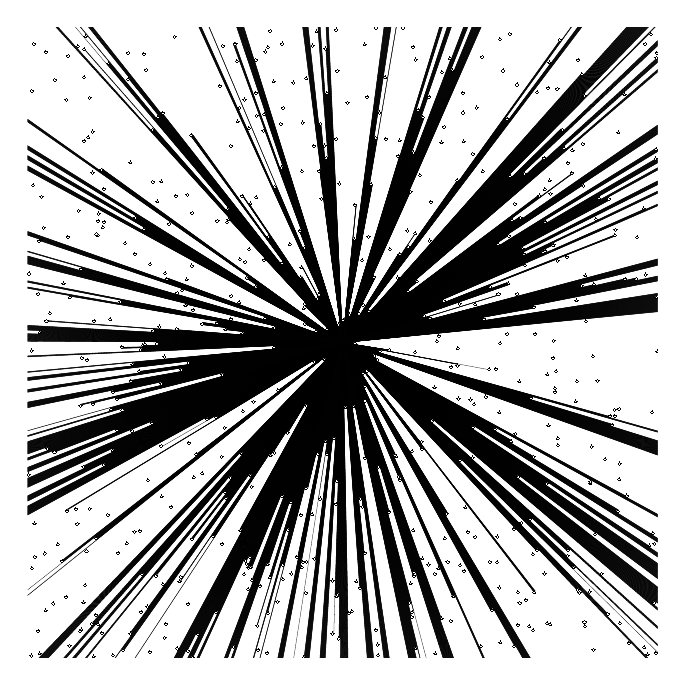
\begin{tikzpicture}[thick,scale=2]
\coordinate (O) at (0,0);

\clip (-2,-2) rectangle (2,2);
\draw[line width=0.1] (0,0)--(0.0790,0.0000);
\draw[line width=0.1] (0,0)--(0.0790,0.0000);
\draw[line width=0.1] (0,0)--(0.0790,0.0001);
\draw[line width=0.1] (0,0)--(0.0790,0.0001);
\draw[line width=0.1] (0,0)--(0.0790,0.0002);
\draw[line width=0.1] (0,0)--(0.0790,0.0002);
\draw[line width=0.1] (0,0)--(0.0790,0.0002);
\draw[line width=0.1] (0,0)--(0.0790,0.0003);
\draw[line width=0.1] (0,0)--(0.0790,0.0003);
\draw[line width=0.1] (0,0)--(0.0790,0.0004);
\draw[line width=0.1] (0,0)--(0.0790,0.0004);
\draw[line width=0.1] (0,0)--(0.0790,0.0004);
\draw[line width=0.1] (0,0)--(0.0790,0.0005);
\draw[line width=0.1] (0,0)--(0.0790,0.0005);
\draw[line width=0.1] (0,0)--(0.0790,0.0006);
\draw[line width=0.1] (0,0)--(0.0790,0.0006);
\draw[line width=0.1] (0,0)--(0.0790,0.0006);
\draw[line width=0.1] (0,0)--(0.0790,0.0007);
\draw[line width=0.1] (0,0)--(0.0790,0.0007);
\draw[line width=0.1] (0,0)--(0.0790,0.0008);
\draw[line width=0.1] (0,0)--(0.0790,0.0008);
\draw[line width=0.1] (0,0)--(0.0790,0.0008);
\draw[line width=0.1] (0,0)--(0.0790,0.0009);
\draw[line width=0.1] (0,0)--(0.0790,0.0009);
\draw[line width=0.1] (0,0)--(0.0790,0.0009);
\draw[line width=0.1] (0,0)--(0.0790,0.0010);
\draw[line width=0.1] (0,0)--(0.0790,0.0010);
\draw[line width=0.1] (0,0)--(0.0790,0.0011);
\draw[line width=0.1] (0,0)--(0.0790,0.0011);
\draw[line width=0.1] (0,0)--(0.0790,0.0011);
\draw[line width=0.1] (0,0)--(0.0790,0.0012);
\draw[line width=0.1] (0,0)--(0.0790,0.0012);
\draw[line width=0.1] (0,0)--(0.0790,0.0013);
\draw[line width=0.1] (0,0)--(0.0790,0.0013);
\draw[line width=0.1] (0,0)--(0.0790,0.0013);
\draw[line width=0.1] (0,0)--(0.0790,0.0014);
\draw[line width=0.1] (0,0)--(0.0790,0.0014);
\draw[line width=0.1] (0,0)--(0.0790,0.0015);
\draw[line width=0.1] (0,0)--(0.0790,0.0015);
\draw[line width=0.1] (0,0)--(0.0790,0.0015);
\draw[line width=0.1] (0,0)--(0.0790,0.0016);
\draw[line width=0.1] (0,0)--(0.0790,0.0016);
\draw[line width=0.1] (0,0)--(0.0790,0.0017);
\draw[line width=0.1] (0,0)--(0.0790,0.0017);
\draw[line width=0.1] (0,0)--(0.0790,0.0017);
\draw[line width=0.1] (0,0)--(0.0790,0.0018);
\draw[line width=0.1] (0,0)--(0.0790,0.0018);
\draw[line width=0.1] (0,0)--(0.0789,0.0019);
\draw[line width=0.1] (0,0)--(0.0789,0.0019);
\draw[line width=0.1] (0,0)--(0.0789,0.0019);
\draw[line width=0.1] (0,0)--(0.0789,0.0020);
\draw[line width=0.1] (0,0)--(0.0789,0.0020);
\draw[line width=0.1] (0,0)--(0.0789,0.0021);
\draw[line width=0.1] (0,0)--(0.0789,0.0021);
\draw[line width=0.1] (0,0)--(0.0789,0.0021);
\draw[line width=0.1] (0,0)--(0.0789,0.0022);
\draw[line width=0.1] (0,0)--(0.0789,0.0022);
\draw[line width=0.1] (0,0)--(0.0789,0.0022);
\draw[line width=0.1] (0,0)--(0.0789,0.0023);
\draw[line width=0.1] (0,0)--(0.0789,0.0023);
\draw[line width=0.1] (0,0)--(0.0789,0.0024);
\draw[line width=0.1] (0,0)--(0.0789,0.0024);
\draw[line width=0.1] (0,0)--(0.0789,0.0024);
\draw[line width=0.1] (0,0)--(0.0789,0.0025);
\draw[line width=0.1] (0,0)--(0.0789,0.0025);
\draw[line width=0.1] (0,0)--(0.0789,0.0026);
\draw[line width=0.1] (0,0)--(0.0789,0.0026);
\draw[line width=0.1] (0,0)--(0.0789,0.0026);
\draw[line width=0.1] (0,0)--(0.0789,0.0027);
\draw[line width=0.1] (0,0)--(0.0789,0.0027);
\draw[line width=0.1] (0,0)--(0.0789,0.0028);
\draw[line width=0.1] (0,0)--(0.0789,0.0028);
\draw[line width=0.1] (0,0)--(0.0789,0.0028);
\draw[line width=0.1] (0,0)--(0.0789,0.0029);
\draw[line width=0.1] (0,0)--(0.0789,0.0029);
\draw[line width=0.1] (0,0)--(0.0788,0.0030);
\draw[line width=0.1] (0,0)--(0.0788,0.0030);
\draw[line width=0.1] (0,0)--(0.0788,0.0030);
\draw[line width=0.1] (0,0)--(0.0788,0.0031);
\draw[line width=0.1] (0,0)--(0.0788,0.0031);
\draw[line width=0.1] (0,0)--(0.0788,0.0032);
\draw[line width=0.1] (0,0)--(0.0788,0.0032);
\draw[line width=0.1] (0,0)--(0.0788,0.0032);
\draw[line width=0.1] (0,0)--(0.0788,0.0033);
\draw[line width=0.1] (0,0)--(0.0788,0.0033);
\draw[line width=0.1] (0,0)--(0.0788,0.0034);
\draw[line width=0.1] (0,0)--(0.0788,0.0034);
\draw[line width=0.1] (0,0)--(0.0788,0.0034);
\draw[line width=0.1] (0,0)--(0.0788,0.0035);
\draw[line width=0.1] (0,0)--(0.0788,0.0035);
\draw[line width=0.1] (0,0)--(0.0788,0.0035);
\draw[line width=0.1] (0,0)--(0.0788,0.0036);
\draw[line width=0.1] (0,0)--(0.0788,0.0036);
\draw[line width=0.1] (0,0)--(0.0788,0.0037);
\draw[line width=0.1] (0,0)--(0.0788,0.0037);
\draw[line width=0.1] (0,0)--(0.0788,0.0037);
\draw[line width=0.1] (0,0)--(0.0788,0.0038);
\draw[line width=0.1] (0,0)--(0.0787,0.0038);
\draw[line width=0.1] (0,0)--(0.0787,0.0039);
\draw[line width=0.1] (0,0)--(0.0787,0.0039);
\draw[line width=0.1] (0,0)--(0.0787,0.0039);
\draw[line width=0.1] (0,0)--(0.0787,0.0040);
\draw[line width=0.1] (0,0)--(0.0787,0.0040);
\draw[line width=0.1] (0,0)--(0.0787,0.0041);
\draw[line width=0.1] (0,0)--(0.0787,0.0041);
\draw[line width=0.1] (0,0)--(0.0787,0.0041);
\draw[line width=0.1] (0,0)--(0.0787,0.0042);
\draw[line width=0.1] (0,0)--(0.0787,0.0042);
\draw[line width=0.1] (0,0)--(0.0787,0.0043);
\draw[line width=0.1] (0,0)--(0.0787,0.0043);
\draw[line width=0.1] (0,0)--(0.0787,0.0043);
\draw[line width=0.1] (0,0)--(0.0787,0.0044);
\draw[line width=0.1] (0,0)--(0.0787,0.0044);
\draw[line width=0.1] (0,0)--(0.0787,0.0044);
\draw[line width=0.1] (0,0)--(0.0787,0.0045);
\draw[line width=0.1] (0,0)--(0.0787,0.0045);
\draw[line width=0.1] (0,0)--(0.0786,0.0046);
\draw[line width=0.1] (0,0)--(0.0786,0.0046);
\draw[line width=0.1] (0,0)--(0.0786,0.0046);
\draw[line width=0.1] (0,0)--(0.0786,0.0047);
\draw[line width=0.1] (0,0)--(0.0786,0.0047);
\draw[line width=0.1] (0,0)--(0.0786,0.0048);
\draw[line width=0.1] (0,0)--(0.0786,0.0048);
\draw[line width=0.1] (0,0)--(0.0786,0.0048);
\draw[line width=0.1] (0,0)--(0.0786,0.0049);
\draw[line width=0.1] (0,0)--(0.0786,0.0049);
\draw[line width=0.1] (0,0)--(0.0786,0.0050);
\draw[line width=0.1] (0,0)--(0.0786,0.0050);
\draw[line width=0.1] (0,0)--(0.0786,0.0050);
\draw[line width=0.1] (0,0)--(0.0786,0.0051);
\draw[line width=0.1] (0,0)--(0.0786,0.0051);
\draw[line width=0.1] (0,0)--(0.0786,0.0052);
\draw[line width=0.1] (0,0)--(0.0785,0.0052);
\draw[line width=0.1] (0,0)--(0.0785,0.0052);
\draw[line width=0.1] (0,0)--(0.0785,0.0053);
\draw[line width=0.1] (0,0)--(0.0785,0.0053);
\draw[line width=0.1] (0,0)--(0.0785,0.0053);
\draw[line width=0.1] (0,0)--(0.0785,0.0054);
\draw[line width=0.1] (0,0)--(0.0785,0.0054);
\draw[line width=0.1] (0,0)--(0.0785,0.0055);
\draw[line width=0.1] (0,0)--(0.0785,0.0055);
\draw[line width=0.1] (0,0)--(0.0785,0.0055);
\draw[line width=0.1] (0,0)--(0.0785,0.0056);
\draw[line width=0.1] (0,0)--(0.0785,0.0056);
\draw[line width=0.1] (0,0)--(0.0785,0.0057);
\draw[line width=0.1] (0,0)--(0.0785,0.0057);
\draw[line width=0.1] (0,0)--(0.0785,0.0057);
\draw[line width=0.1] (0,0)--(0.0784,0.0058);
\draw[line width=0.1] (0,0)--(0.0784,0.0058);
\draw[line width=0.1] (0,0)--(0.0784,0.0059);
\draw[line width=0.1] (0,0)--(0.0784,0.0059);
\draw[line width=0.1] (0,0)--(0.0784,0.0059);
\draw[line width=0.1] (0,0)--(0.0784,0.0060);
\draw[line width=0.1] (0,0)--(0.0784,0.0060);
\draw[line width=0.1] (0,0)--(0.0784,0.0060);
\draw[line width=0.1] (0,0)--(0.0784,0.0061);
\draw[line width=0.1] (0,0)--(0.0784,0.0061);
\draw[line width=0.1] (0,0)--(0.0784,0.0062);
\draw[line width=0.1] (0,0)--(0.0784,0.0062);
\draw[line width=0.1] (0,0)--(0.0784,0.0062);
\draw[line width=0.1] (0,0)--(0.0784,0.0063);
\draw[line width=0.1] (0,0)--(0.0783,0.0063);
\draw[line width=0.1] (0,0)--(0.0783,0.0064);
\draw[line width=0.1] (0,0)--(0.0783,0.0064);
\draw[line width=0.1] (0,0)--(0.0783,0.0064);
\draw[line width=0.1] (0,0)--(0.0783,0.0065);
\draw[line width=0.1] (0,0)--(0.0783,0.0065);
\draw[line width=0.1] (0,0)--(0.0783,0.0066);
\draw[line width=0.1] (0,0)--(0.0783,0.0066);
\draw[line width=0.1] (0,0)--(0.0783,0.0066);
\draw[line width=0.1] (0,0)--(0.0783,0.0067);
\draw[line width=0.1] (0,0)--(0.0783,0.0067);
\draw[line width=0.1] (0,0)--(0.0783,0.0067);
\draw[line width=0.1] (0,0)--(0.0783,0.0068);
\draw[line width=0.1] (0,0)--(0.0782,0.0068);
\draw[line width=0.1] (0,0)--(0.0782,0.0069);
\draw[line width=0.1] (0,0)--(0.0782,0.0069);
\draw[line width=0.1] (0,0)--(0.0782,0.0069);
\draw[line width=0.1] (0,0)--(0.0782,0.0070);
\draw[line width=0.1] (0,0)--(0.0782,0.0070);
\draw[line width=0.1] (0,0)--(0.0782,0.0071);
\draw[line width=0.1] (0,0)--(0.0782,0.0071);
\draw[line width=0.1] (0,0)--(0.0782,0.0071);
\draw[line width=0.1] (0,0)--(0.0782,0.0072);
\draw[line width=0.1] (0,0)--(0.0782,0.0072);
\draw[line width=0.1] (0,0)--(0.0782,0.0073);
\draw[line width=0.1] (0,0)--(0.0781,0.0073);
\draw[line width=0.1] (0,0)--(0.0781,0.0073);
\draw[line width=0.1] (0,0)--(0.0781,0.0074);
\draw[line width=0.1] (0,0)--(0.0781,0.0074);
\draw[line width=0.1] (0,0)--(0.0781,0.0074);
\draw[line width=0.1] (0,0)--(0.0781,0.0075);
\draw[line width=0.1] (0,0)--(0.0781,0.0075);
\draw[line width=0.1] (0,0)--(0.0781,0.0076);
\draw[line width=0.1] (0,0)--(0.0781,0.0076);
\draw[line width=0.1] (0,0)--(9.9525,0.9735);
\draw[line width=0.1] (0,0)--(9.9520,0.9784);
\draw[line width=0.1] (0,0)--(9.9515,0.9834);
\draw[line width=0.1] (0,0)--(9.9510,0.9884);
\draw[line width=0.1] (0,0)--(9.9505,0.9934);
\draw[line width=0.1] (0,0)--(9.9500,0.9983);
\draw[line width=0.1] (0,0)--(9.9495,1.0033);
\draw[line width=0.1] (0,0)--(9.9490,1.0083);
\draw[line width=0.1] (0,0)--(9.9485,1.0133);
\draw[line width=0.1] (0,0)--(9.9480,1.0182);
\draw[line width=0.1] (0,0)--(9.9475,1.0232);
\draw[line width=0.1] (0,0)--(9.9470,1.0282);
\draw[line width=0.1] (0,0)--(9.9465,1.0332);
\draw[line width=0.1] (0,0)--(9.9460,1.0381);
\draw[line width=0.1] (0,0)--(9.9454,1.0431);
\draw[line width=0.1] (0,0)--(9.9449,1.0481);
\draw[line width=0.1] (0,0)--(9.9444,1.0530);
\draw[line width=0.1] (0,0)--(9.9439,1.0580);
\draw[line width=0.1] (0,0)--(9.9433,1.0630);
\draw[line width=0.1] (0,0)--(9.9428,1.0680);
\draw[line width=0.1] (0,0)--(9.9423,1.0729);
\draw[line width=0.1] (0,0)--(9.9417,1.0779);
\draw[line width=0.1] (0,0)--(9.9412,1.0829);
\draw[line width=0.1] (0,0)--(9.9407,1.0878);
\draw[line width=0.1] (0,0)--(9.9401,1.0928);
\draw[line width=0.1] (0,0)--(9.9396,1.0978);
\draw[line width=0.1] (0,0)--(9.9390,1.1028);
\draw[line width=0.1] (0,0)--(9.9385,1.1077);
\draw[line width=0.1] (0,0)--(9.9379,1.1127);
\draw[line width=0.1] (0,0)--(9.9373,1.1177);
\draw[line width=0.1] (0,0)--(9.9368,1.1226);
\draw[line width=0.1] (0,0)--(9.9362,1.1276);
\draw[line width=0.1] (0,0)--(9.9357,1.1326);
\draw[line width=0.1] (0,0)--(9.9351,1.1375);
\draw[line width=0.1] (0,0)--(9.9345,1.1425);
\draw[line width=0.1] (0,0)--(9.9339,1.1475);
\draw[line width=0.1] (0,0)--(9.9334,1.1524);
\draw[line width=0.1] (0,0)--(9.9328,1.1574);
\draw[line width=0.1] (0,0)--(9.9322,1.1624);
\draw[line width=0.1] (0,0)--(9.9316,1.1673);
\draw[line width=0.1] (0,0)--(9.9310,1.1723);
\draw[line width=0.1] (0,0)--(9.9305,1.1773);
\draw[line width=0.1] (0,0)--(9.9299,1.1822);
\draw[line width=0.1] (0,0)--(9.9293,1.1872);
\draw[line width=0.1] (0,0)--(9.9287,1.1922);
\draw[line width=0.1] (0,0)--(9.9281,1.1971);
\draw[line width=0.1] (0,0)--(9.9275,1.2021);
\draw[line width=0.1] (0,0)--(9.9269,1.2070);
\draw[line width=0.1] (0,0)--(9.9263,1.2120);
\draw[line width=0.1] (0,0)--(9.9257,1.2170);
\draw[line width=0.1] (0,0)--(9.9251,1.2219);
\draw[line width=0.1] (0,0)--(9.9245,1.2269);
\draw[line width=0.1] (0,0)--(9.9238,1.2319);
\draw[line width=0.1] (0,0)--(9.9232,1.2368);
\draw[line width=0.1] (0,0)--(9.9226,1.2418);
\draw[line width=0.1] (0,0)--(9.9220,1.2467);
\draw[line width=0.1] (0,0)--(9.9214,1.2517);
\draw[line width=0.1] (0,0)--(9.9207,1.2567);
\draw[line width=0.1] (0,0)--(9.9201,1.2616);
\draw[line width=0.1] (0,0)--(9.9195,1.2666);
\draw[line width=0.1] (0,0)--(9.9188,1.2715);
\draw[line width=0.1] (0,0)--(9.9182,1.2765);
\draw[line width=0.1] (0,0)--(9.9176,1.2815);
\draw[line width=0.1] (0,0)--(9.9169,1.2864);
\draw[line width=0.1] (0,0)--(9.9163,1.2914);
\draw[line width=0.1] (0,0)--(9.9156,1.2963);
\draw[line width=0.1] (0,0)--(9.9150,1.3013);
\draw[line width=0.1] (0,0)--(9.9143,1.3063);
\draw[line width=0.1] (0,0)--(9.9137,1.3112);
\draw[line width=0.1] (0,0)--(9.9130,1.3162);
\draw[line width=0.1] (0,0)--(9.9123,1.3211);
\draw[line width=0.1] (0,0)--(9.9117,1.3261);
\draw[line width=0.1] (0,0)--(9.9110,1.3310);
\draw[line width=0.1] (0,0)--(9.9104,1.3360);
\draw[line width=0.1] (0,0)--(9.9097,1.3409);
\draw[line width=0.1] (0,0)--(9.9090,1.3459);
\draw[line width=0.1] (0,0)--(9.9083,1.3509);
\draw[line width=0.1] (0,0)--(9.9077,1.3558);
\draw[line width=0.1] (0,0)--(9.9070,1.3608);
\draw[line width=0.1] (0,0)--(9.9063,1.3657);
\draw[line width=0.1] (0,0)--(9.9056,1.3707);
\draw[line width=0.1] (0,0)--(9.9049,1.3756);
\draw[line width=0.1] (0,0)--(1.9947,0.2781);
\draw[line width=0.1] (0,0)--(1.9946,0.2790);
\draw[line width=0.1] (0,0)--(1.9945,0.2800);
\draw[line width=0.1] (0,0)--(1.9943,0.2810);
\draw[line width=0.1] (0,0)--(1.9942,0.2820);
\draw[line width=0.1] (0,0)--(1.9941,0.2830);
\draw[line width=0.1] (0,0)--(1.9939,0.2840);
\draw[line width=0.1] (0,0)--(1.9938,0.2850);
\draw[line width=0.1] (0,0)--(1.9936,0.2860);
\draw[line width=0.1] (0,0)--(1.9935,0.2870);
\draw[line width=0.1] (0,0)--(1.9933,0.2880);
\draw[line width=0.1] (0,0)--(1.9932,0.2890);
\draw[line width=0.1] (0,0)--(1.9931,0.2900);
\draw[line width=0.1] (0,0)--(1.9929,0.2910);
\draw[line width=0.1] (0,0)--(1.9928,0.2920);
\draw[line width=0.1] (0,0)--(1.9926,0.2930);
\draw[line width=0.1] (0,0)--(1.9925,0.2940);
\draw[line width=0.1] (0,0)--(1.9923,0.2950);
\draw[line width=0.1] (0,0)--(1.9922,0.2960);
\draw[line width=0.1] (0,0)--(1.9920,0.2970);
\draw[line width=0.1] (0,0)--(9.8899,1.4795);
\draw[line width=0.1] (0,0)--(9.8892,1.4845);
\draw[line width=0.1] (0,0)--(9.8885,1.4894);
\draw[line width=0.1] (0,0)--(9.8877,1.4944);
\draw[line width=0.1] (0,0)--(9.8870,1.4993);
\draw[line width=0.1] (0,0)--(9.8862,1.5043);
\draw[line width=0.1] (0,0)--(9.8855,1.5092);
\draw[line width=0.1] (0,0)--(9.8847,1.5142);
\draw[line width=0.1] (0,0)--(9.8839,1.5191);
\draw[line width=0.1] (0,0)--(9.8832,1.5240);
\draw[line width=0.1] (0,0)--(9.8824,1.5290);
\draw[line width=0.1] (0,0)--(9.8817,1.5339);
\draw[line width=0.1] (0,0)--(9.8809,1.5389);
\draw[line width=0.1] (0,0)--(9.8801,1.5438);
\draw[line width=0.1] (0,0)--(9.8793,1.5487);
\draw[line width=0.1] (0,0)--(0.8983,0.1413);
\draw[line width=0.1] (0,0)--(0.8982,0.1417);
\draw[line width=0.1] (0,0)--(0.8981,0.1422);
\draw[line width=0.1] (0,0)--(0.8981,0.1426);
\draw[line width=0.1] (0,0)--(0.8980,0.1431);
\draw[line width=0.1] (0,0)--(0.8979,0.1435);
\draw[line width=0.1] (0,0)--(0.8979,0.1440);
\draw[line width=0.1] (0,0)--(0.8978,0.1444);
\draw[line width=0.1] (0,0)--(0.8977,0.1449);
\draw[line width=0.1] (0,0)--(0.8977,0.1453);
\draw[line width=0.1] (0,0)--(0.8976,0.1458);
\draw[line width=0.1] (0,0)--(0.8975,0.1462);
\draw[line width=0.1] (0,0)--(0.8974,0.1467);
\draw[line width=0.1] (0,0)--(0.8974,0.1471);
\draw[line width=0.1] (0,0)--(0.8973,0.1476);
\draw[line width=0.1] (0,0)--(0.8972,0.1480);
\draw[line width=0.1] (0,0)--(0.8972,0.1485);
\draw[line width=0.1] (0,0)--(0.8971,0.1489);
\draw[line width=0.1] (0,0)--(0.8970,0.1494);
\draw[line width=0.1] (0,0)--(0.8969,0.1498);
\draw[line width=0.1] (0,0)--(0.8969,0.1503);
\draw[line width=0.1] (0,0)--(0.8968,0.1507);
\draw[line width=0.1] (0,0)--(0.8967,0.1512);
\draw[line width=0.1] (0,0)--(0.8966,0.1516);
\draw[line width=0.1] (0,0)--(0.8966,0.1521);
\draw[line width=0.1] (0,0)--(0.8965,0.1525);
\draw[line width=0.1] (0,0)--(0.8964,0.1530);
\draw[line width=0.1] (0,0)--(0.8963,0.1534);
\draw[line width=0.1] (0,0)--(0.8962,0.1538);
\draw[line width=0.1] (0,0)--(0.8962,0.1543);
\draw[line width=0.1] (0,0)--(0.8961,0.1547);
\draw[line width=0.1] (0,0)--(0.8960,0.1552);
\draw[line width=0.1] (0,0)--(0.8959,0.1556);
\draw[line width=0.1] (0,0)--(0.8959,0.1561);
\draw[line width=0.1] (0,0)--(0.8958,0.1565);
\draw[line width=0.1] (0,0)--(0.8957,0.1570);
\draw[line width=0.1] (0,0)--(0.8956,0.1574);
\draw[line width=0.1] (0,0)--(0.8955,0.1579);
\draw[line width=0.1] (0,0)--(0.8954,0.1583);
\draw[line width=0.1] (0,0)--(0.8954,0.1588);
\draw[line width=0.1] (0,0)--(0.8953,0.1592);
\draw[line width=0.1] (0,0)--(0.8952,0.1597);
\draw[line width=0.1] (0,0)--(0.8951,0.1601);
\draw[line width=0.1] (0,0)--(0.8950,0.1606);
\draw[line width=0.1] (0,0)--(1.2162,0.2188);
\draw[line width=0.1] (0,0)--(1.2161,0.2194);
\draw[line width=0.1] (0,0)--(1.2160,0.2200);
\draw[line width=0.1] (0,0)--(1.2159,0.2206);
\draw[line width=0.1] (0,0)--(1.2158,0.2212);
\draw[line width=0.1] (0,0)--(1.2157,0.2218);
\draw[line width=0.1] (0,0)--(1.2155,0.2224);
\draw[line width=0.1] (0,0)--(1.2154,0.2231);
\draw[line width=0.1] (0,0)--(1.2153,0.2237);
\draw[line width=0.1] (0,0)--(1.2152,0.2243);
\draw[line width=0.1] (0,0)--(1.2151,0.2249);
\draw[line width=0.1] (0,0)--(1.2150,0.2255);
\draw[line width=0.1] (0,0)--(1.2149,0.2261);
\draw[line width=0.1] (0,0)--(1.2148,0.2267);
\draw[line width=0.1] (0,0)--(1.2147,0.2273);
\draw[line width=0.1] (0,0)--(1.2145,0.2279);
\draw[line width=0.1] (0,0)--(1.2144,0.2285);
\draw[line width=0.1] (0,0)--(1.2143,0.2291);
\draw[line width=0.1] (0,0)--(1.2142,0.2297);
\draw[line width=0.1] (0,0)--(1.2141,0.2303);
\draw[line width=0.1] (0,0)--(1.2140,0.2310);
\draw[line width=0.1] (0,0)--(1.2138,0.2316);
\draw[line width=0.1] (0,0)--(1.2137,0.2322);
\draw[line width=0.1] (0,0)--(1.2136,0.2328);
\draw[line width=0.1] (0,0)--(1.2135,0.2334);
\draw[line width=0.1] (0,0)--(1.2134,0.2340);
\draw[line width=0.1] (0,0)--(1.2132,0.2346);
\draw[line width=0.1] (0,0)--(1.2131,0.2352);
\draw[line width=0.1] (0,0)--(1.2130,0.2358);
\draw[line width=0.1] (0,0)--(1.2129,0.2364);
\draw[line width=0.1] (0,0)--(9.8143,1.9180);
\draw[line width=0.1] (0,0)--(9.8134,1.9229);
\draw[line width=0.1] (0,0)--(9.8124,1.9279);
\draw[line width=0.1] (0,0)--(9.8114,1.9328);
\draw[line width=0.1] (0,0)--(9.8105,1.9377);
\draw[line width=0.1] (0,0)--(9.8095,1.9426);
\draw[line width=0.1] (0,0)--(9.8085,1.9475);
\draw[line width=0.1] (0,0)--(9.8076,1.9524);
\draw[line width=0.1] (0,0)--(9.8066,1.9573);
\draw[line width=0.1] (0,0)--(9.8056,1.9622);
\draw[line width=0.1] (0,0)--(9.8046,1.9671);
\draw[line width=0.1] (0,0)--(9.8036,1.9720);
\draw[line width=0.1] (0,0)--(9.8026,1.9769);
\draw[line width=0.1] (0,0)--(9.8017,1.9818);
\draw[line width=0.1] (0,0)--(9.8007,1.9867);
\draw[line width=0.1] (0,0)--(9.7997,1.9916);
\draw[line width=0.1] (0,0)--(9.7987,1.9965);
\draw[line width=0.1] (0,0)--(9.7977,2.0014);
\draw[line width=0.1] (0,0)--(9.7967,2.0063);
\draw[line width=0.1] (0,0)--(9.7957,2.0112);
\draw[line width=0.1] (0,0)--(9.7947,2.0161);
\draw[line width=0.1] (0,0)--(9.7937,2.0210);
\draw[line width=0.1] (0,0)--(9.7926,2.0259);
\draw[line width=0.1] (0,0)--(9.7916,2.0308);
\draw[line width=0.1] (0,0)--(9.7906,2.0357);
\draw[line width=0.1] (0,0)--(9.7896,2.0406);
\draw[line width=0.1] (0,0)--(9.7886,2.0455);
\draw[line width=0.1] (0,0)--(9.7875,2.0504);
\draw[line width=0.1] (0,0)--(9.7865,2.0552);
\draw[line width=0.1] (0,0)--(9.7855,2.0601);
\draw[line width=0.1] (0,0)--(9.7845,2.0650);
\draw[line width=0.1] (0,0)--(9.7834,2.0699);
\draw[line width=0.1] (0,0)--(1.8672,0.3960);
\draw[line width=0.1] (0,0)--(1.8670,0.3970);
\draw[line width=0.1] (0,0)--(1.8668,0.3979);
\draw[line width=0.1] (0,0)--(1.8666,0.3988);
\draw[line width=0.1] (0,0)--(1.8664,0.3998);
\draw[line width=0.1] (0,0)--(1.8662,0.4007);
\draw[line width=0.1] (0,0)--(1.8660,0.4016);
\draw[line width=0.1] (0,0)--(1.8658,0.4026);
\draw[line width=0.1] (0,0)--(1.8656,0.4035);
\draw[line width=0.1] (0,0)--(1.8654,0.4044);
\draw[line width=0.1] (0,0)--(1.8652,0.4054);
\draw[line width=0.1] (0,0)--(1.8650,0.4063);
\draw[line width=0.1] (0,0)--(1.8648,0.4072);
\draw[line width=0.1] (0,0)--(1.8646,0.4082);
\draw[line width=0.1] (0,0)--(1.8644,0.4091);
\draw[line width=0.1] (0,0)--(1.8642,0.4100);
\draw[line width=0.1] (0,0)--(1.8640,0.4110);
\draw[line width=0.1] (0,0)--(1.7951,0.3967);
\draw[line width=0.1] (0,0)--(1.7949,0.3976);
\draw[line width=0.1] (0,0)--(1.7947,0.3985);
\draw[line width=0.1] (0,0)--(1.7945,0.3994);
\draw[line width=0.1] (0,0)--(1.7943,0.4003);
\draw[line width=0.1] (0,0)--(1.7941,0.4012);
\draw[line width=0.1] (0,0)--(1.7939,0.4021);
\draw[line width=0.1] (0,0)--(1.7937,0.4030);
\draw[line width=0.1] (0,0)--(1.7935,0.4039);
\draw[line width=0.1] (0,0)--(1.7933,0.4048);
\draw[line width=0.1] (0,0)--(1.7931,0.4057);
\draw[line width=0.1] (0,0)--(1.5971,0.3622);
\draw[line width=0.1] (0,0)--(1.5969,0.3630);
\draw[line width=0.1] (0,0)--(1.5967,0.3638);
\draw[line width=0.1] (0,0)--(1.5966,0.3646);
\draw[line width=0.1] (0,0)--(1.5964,0.3654);
\draw[line width=0.1] (0,0)--(1.5962,0.3662);
\draw[line width=0.1] (0,0)--(1.5960,0.3670);
\draw[line width=0.1] (0,0)--(1.5958,0.3678);
\draw[line width=0.1] (0,0)--(1.5956,0.3686);
\draw[line width=0.1] (0,0)--(1.5201,0.3519);
\draw[line width=0.1] (0,0)--(1.5199,0.3527);
\draw[line width=0.1] (0,0)--(1.5197,0.3534);
\draw[line width=0.1] (0,0)--(1.5196,0.3542);
\draw[line width=0.1] (0,0)--(1.5194,0.3550);
\draw[line width=0.1] (0,0)--(1.5192,0.3557);
\draw[line width=0.1] (0,0)--(1.5190,0.3565);
\draw[line width=0.1] (0,0)--(1.5189,0.3572);
\draw[line width=0.1] (0,0)--(1.5187,0.3580);
\draw[line width=0.1] (0,0)--(1.5185,0.3588);
\draw[line width=0.1] (0,0)--(1.5183,0.3595);
\draw[line width=0.1] (0,0)--(1.5181,0.3603);
\draw[line width=0.1] (0,0)--(1.5180,0.3610);
\draw[line width=0.1] (0,0)--(1.5178,0.3618);
\draw[line width=0.1] (0,0)--(1.5176,0.3625);
\draw[line width=0.1] (0,0)--(1.5174,0.3633);
\draw[line width=0.1] (0,0)--(1.5172,0.3641);
\draw[line width=0.1] (0,0)--(1.5171,0.3648);
\draw[line width=0.1] (0,0)--(1.5169,0.3656);
\draw[line width=0.1] (0,0)--(1.5167,0.3663);
\draw[line width=0.1] (0,0)--(1.5165,0.3671);
\draw[line width=0.1] (0,0)--(1.5163,0.3679);
\draw[line width=0.1] (0,0)--(1.5161,0.3686);
\draw[line width=0.1] (0,0)--(1.5159,0.3694);
\draw[line width=0.1] (0,0)--(1.5158,0.3701);
\draw[line width=0.1] (0,0)--(1.5156,0.3709);
\draw[line width=0.1] (0,0)--(9.7122,2.3819);
\draw[line width=0.1] (0,0)--(9.7110,2.3867);
\draw[line width=0.1] (0,0)--(9.7098,2.3916);
\draw[line width=0.1] (0,0)--(9.7086,2.3964);
\draw[line width=0.1] (0,0)--(9.7074,2.4013);
\draw[line width=0.1] (0,0)--(9.7062,2.4062);
\draw[line width=0.1] (0,0)--(9.7050,2.4110);
\draw[line width=0.1] (0,0)--(9.7038,2.4159);
\draw[line width=0.1] (0,0)--(9.7026,2.4207);
\draw[line width=0.1] (0,0)--(9.7014,2.4256);
\draw[line width=0.1] (0,0)--(9.7002,2.4304);
\draw[line width=0.1] (0,0)--(9.6989,2.4353);
\draw[line width=0.1] (0,0)--(9.6977,2.4401);
\draw[line width=0.1] (0,0)--(9.6965,2.4450);
\draw[line width=0.1] (0,0)--(9.6953,2.4498);
\draw[line width=0.1] (0,0)--(9.6941,2.4547);
\draw[line width=0.1] (0,0)--(9.6928,2.4595);
\draw[line width=0.1] (0,0)--(9.6916,2.4643);
\draw[line width=0.1] (0,0)--(9.6904,2.4692);
\draw[line width=0.1] (0,0)--(9.6891,2.4740);
\draw[line width=0.1] (0,0)--(9.6879,2.4789);
\draw[line width=0.1] (0,0)--(9.6866,2.4837);
\draw[line width=0.1] (0,0)--(9.6854,2.4886);
\draw[line width=0.1] (0,0)--(9.6842,2.4934);
\draw[line width=0.1] (0,0)--(9.6829,2.4983);
\draw[line width=0.1] (0,0)--(9.6817,2.5031);
\draw[line width=0.1] (0,0)--(9.6804,2.5079);
\draw[line width=0.1] (0,0)--(9.6792,2.5128);
\draw[line width=0.1] (0,0)--(9.6779,2.5176);
\draw[line width=0.1] (0,0)--(9.6766,2.5225);
\draw[line width=0.1] (0,0)--(9.6754,2.5273);
\draw[line width=0.1] (0,0)--(9.6741,2.5321);
\draw[line width=0.1] (0,0)--(9.6728,2.5370);
\draw[line width=0.1] (0,0)--(9.6716,2.5418);
\draw[line width=0.1] (0,0)--(9.6703,2.5466);
\draw[line width=0.1] (0,0)--(9.6690,2.5515);
\draw[line width=0.1] (0,0)--(9.6677,2.5563);
\draw[line width=0.1] (0,0)--(9.6665,2.5611);
\draw[line width=0.1] (0,0)--(9.6652,2.5660);
\draw[line width=0.1] (0,0)--(9.6639,2.5708);
\draw[line width=0.1] (0,0)--(0.5565,0.1483);
\draw[line width=0.1] (0,0)--(0.5564,0.1486);
\draw[line width=0.1] (0,0)--(0.5563,0.1489);
\draw[line width=0.1] (0,0)--(0.5563,0.1492);
\draw[line width=0.1] (0,0)--(0.5562,0.1495);
\draw[line width=0.1] (0,0)--(0.5561,0.1497);
\draw[line width=0.1] (0,0)--(0.5561,0.1500);
\draw[line width=0.1] (0,0)--(0.5560,0.1503);
\draw[line width=0.1] (0,0)--(0.5559,0.1506);
\draw[line width=0.1] (0,0)--(0.5558,0.1508);
\draw[line width=0.1] (0,0)--(0.5558,0.1511);
\draw[line width=0.1] (0,0)--(0.5557,0.1514);
\draw[line width=0.1] (0,0)--(0.5556,0.1517);
\draw[line width=0.1] (0,0)--(0.5556,0.1520);
\draw[line width=0.1] (0,0)--(0.5555,0.1522);
\draw[line width=0.1] (0,0)--(0.5554,0.1525);
\draw[line width=0.1] (0,0)--(0.5553,0.1528);
\draw[line width=0.1] (0,0)--(0.5553,0.1531);
\draw[line width=0.1] (0,0)--(0.5552,0.1534);
\draw[line width=0.1] (0,0)--(0.5551,0.1536);
\draw[line width=0.1] (0,0)--(0.5550,0.1539);
\draw[line width=0.1] (0,0)--(0.5550,0.1542);
\draw[line width=0.1] (0,0)--(0.5549,0.1545);
\draw[line width=0.1] (0,0)--(0.5548,0.1547);
\draw[line width=0.1] (0,0)--(0.5547,0.1550);
\draw[line width=0.1] (0,0)--(0.5547,0.1553);
\draw[line width=0.1] (0,0)--(0.5546,0.1556);
\draw[line width=0.1] (0,0)--(0.5545,0.1559);
\draw[line width=0.1] (0,0)--(0.5544,0.1561);
\draw[line width=0.1] (0,0)--(0.5544,0.1564);
\draw[line width=0.1] (0,0)--(0.5543,0.1567);
\draw[line width=0.1] (0,0)--(0.5542,0.1570);
\draw[line width=0.1] (0,0)--(0.5541,0.1572);
\draw[line width=0.1] (0,0)--(0.5540,0.1575);
\draw[line width=0.1] (0,0)--(0.5540,0.1578);
\draw[line width=0.1] (0,0)--(0.5539,0.1581);
\draw[line width=0.1] (0,0)--(0.5538,0.1583);
\draw[line width=0.1] (0,0)--(0.5537,0.1586);
\draw[line width=0.1] (0,0)--(0.5536,0.1589);
\draw[line width=0.1] (0,0)--(0.5536,0.1592);
\draw[line width=0.1] (0,0)--(0.5535,0.1595);
\draw[line width=0.1] (0,0)--(0.5534,0.1597);
\draw[line width=0.1] (0,0)--(0.5533,0.1600);
\draw[line width=0.1] (0,0)--(0.5532,0.1603);
\draw[line width=0.1] (0,0)--(0.5532,0.1606);
\draw[line width=0.1] (0,0)--(0.5531,0.1608);
\draw[line width=0.1] (0,0)--(0.5530,0.1611);
\draw[line width=0.1] (0,0)--(0.5529,0.1614);
\draw[line width=0.1] (0,0)--(0.5528,0.1617);
\draw[line width=0.1] (0,0)--(0.5527,0.1619);
\draw[line width=0.1] (0,0)--(0.5527,0.1622);
\draw[line width=0.1] (0,0)--(0.5526,0.1625);
\draw[line width=0.1] (0,0)--(0.5525,0.1628);
\draw[line width=0.1] (0,0)--(0.5524,0.1630);
\draw[line width=0.1] (0,0)--(0.5523,0.1633);
\draw[line width=0.1] (0,0)--(0.5522,0.1636);
\draw[line width=0.1] (0,0)--(0.5522,0.1639);
\draw[line width=0.1] (0,0)--(0.5521,0.1641);
\draw[line width=0.1] (0,0)--(0.5520,0.1644);
\draw[line width=0.1] (0,0)--(0.5519,0.1647);
\draw[line width=0.1] (0,0)--(0.5518,0.1650);
\draw[line width=0.1] (0,0)--(0.5517,0.1652);
\draw[line width=0.1] (0,0)--(0.5516,0.1655);
\draw[line width=0.1] (0,0)--(0.5516,0.1658);
\draw[line width=0.1] (0,0)--(0.5515,0.1661);
\draw[line width=0.1] (0,0)--(0.5514,0.1663);
\draw[line width=0.1] (0,0)--(0.5513,0.1666);
\draw[line width=0.1] (0,0)--(0.5512,0.1669);
\draw[line width=0.1] (0,0)--(0.5511,0.1672);
\draw[line width=0.1] (0,0)--(0.5510,0.1674);
\draw[line width=0.1] (0,0)--(0.9917,0.3019);
\draw[line width=0.1] (0,0)--(0.9915,0.3024);
\draw[line width=0.1] (0,0)--(0.9914,0.3029);
\draw[line width=0.1] (0,0)--(0.9912,0.3034);
\draw[line width=0.1] (0,0)--(0.9911,0.3039);
\draw[line width=0.1] (0,0)--(0.5223,0.1604);
\draw[line width=0.1] (0,0)--(0.5222,0.1607);
\draw[line width=0.1] (0,0)--(0.5221,0.1609);
\draw[line width=0.1] (0,0)--(0.5220,0.1612);
\draw[line width=0.1] (0,0)--(0.5220,0.1615);
\draw[line width=0.1] (0,0)--(0.5219,0.1617);
\draw[line width=0.1] (0,0)--(0.5218,0.1620);
\draw[line width=0.1] (0,0)--(0.5217,0.1622);
\draw[line width=0.1] (0,0)--(0.5217,0.1625);
\draw[line width=0.1] (0,0)--(0.5216,0.1628);
\draw[line width=0.1] (0,0)--(0.5215,0.1630);
\draw[line width=0.1] (0,0)--(0.5214,0.1633);
\draw[line width=0.1] (0,0)--(0.5213,0.1636);
\draw[line width=0.1] (0,0)--(0.5213,0.1638);
\draw[line width=0.1] (0,0)--(0.5212,0.1641);
\draw[line width=0.1] (0,0)--(0.5211,0.1643);
\draw[line width=0.1] (0,0)--(0.5210,0.1646);
\draw[line width=0.1] (0,0)--(0.5209,0.1649);
\draw[line width=0.1] (0,0)--(0.5209,0.1651);
\draw[line width=0.1] (0,0)--(0.5208,0.1654);
\draw[line width=0.1] (0,0)--(0.5207,0.1656);
\draw[line width=0.1] (0,0)--(0.5206,0.1659);
\draw[line width=0.1] (0,0)--(0.5205,0.1662);
\draw[line width=0.1] (0,0)--(0.5205,0.1664);
\draw[line width=0.1] (0,0)--(0.5204,0.1667);
\draw[line width=0.1] (0,0)--(0.5203,0.1670);
\draw[line width=0.1] (0,0)--(0.5202,0.1672);
\draw[line width=0.1] (0,0)--(0.5201,0.1675);
\draw[line width=0.1] (0,0)--(0.5201,0.1677);
\draw[line width=0.1] (0,0)--(0.5200,0.1680);
\draw[line width=0.1] (0,0)--(0.5199,0.1683);
\draw[line width=0.1] (0,0)--(0.5198,0.1685);
\draw[line width=0.1] (0,0)--(0.5197,0.1688);
\draw[line width=0.1] (0,0)--(0.5196,0.1690);
\draw[line width=0.1] (0,0)--(0.5195,0.1693);
\draw[line width=0.1] (0,0)--(0.5195,0.1696);
\draw[line width=0.1] (0,0)--(0.5194,0.1698);
\draw[line width=0.1] (0,0)--(0.5193,0.1701);
\draw[line width=0.1] (0,0)--(0.5192,0.1703);
\draw[line width=0.1] (0,0)--(0.5191,0.1706);
\draw[line width=0.1] (0,0)--(0.5190,0.1709);
\draw[line width=0.1] (0,0)--(0.5190,0.1711);
\draw[line width=0.1] (0,0)--(0.5189,0.1714);
\draw[line width=0.1] (0,0)--(0.5188,0.1716);
\draw[line width=0.1] (0,0)--(0.5187,0.1719);
\draw[line width=0.1] (0,0)--(0.5186,0.1721);
\draw[line width=0.1] (0,0)--(0.5185,0.1724);
\draw[line width=0.1] (0,0)--(0.5184,0.1727);
\draw[line width=0.1] (0,0)--(0.5183,0.1729);
\draw[line width=0.1] (0,0)--(0.5183,0.1732);
\draw[line width=0.1] (0,0)--(0.5182,0.1734);
\draw[line width=0.1] (0,0)--(0.5181,0.1737);
\draw[line width=0.1] (0,0)--(0.5180,0.1740);
\draw[line width=0.1] (0,0)--(0.5179,0.1742);
\draw[line width=0.1] (0,0)--(0.5178,0.1745);
\draw[line width=0.1] (0,0)--(0.5177,0.1747);
\draw[line width=0.1] (0,0)--(0.5176,0.1750);
\draw[line width=0.1] (0,0)--(0.5175,0.1752);
\draw[line width=0.1] (0,0)--(0.5175,0.1755);
\draw[line width=0.1] (0,0)--(0.5174,0.1758);
\draw[line width=0.1] (0,0)--(0.5173,0.1760);
\draw[line width=0.1] (0,0)--(0.5172,0.1763);
\draw[line width=0.1] (0,0)--(0.5171,0.1765);
\draw[line width=0.1] (0,0)--(0.5170,0.1768);
\draw[line width=0.1] (0,0)--(0.5169,0.1771);
\draw[line width=0.1] (0,0)--(0.5168,0.1773);
\draw[line width=0.1] (0,0)--(0.5167,0.1776);
\draw[line width=0.1] (0,0)--(0.5166,0.1778);
\draw[line width=0.1] (0,0)--(0.5165,0.1781);
\draw[line width=0.1] (0,0)--(0.5164,0.1783);
\draw[line width=0.1] (0,0)--(0.5163,0.1786);
\draw[line width=0.1] (0,0)--(0.5163,0.1789);
\draw[line width=0.1] (0,0)--(0.5162,0.1791);
\draw[line width=0.1] (0,0)--(0.5161,0.1794);
\draw[line width=0.1] (0,0)--(1.0557,0.3675);
\draw[line width=0.1] (0,0)--(1.0555,0.3680);
\draw[line width=0.1] (0,0)--(1.0554,0.3686);
\draw[line width=0.1] (0,0)--(1.0552,0.3691);
\draw[line width=0.1] (0,0)--(1.0550,0.3696);
\draw[line width=0.1] (0,0)--(1.0548,0.3702);
\draw[line width=0.1] (0,0)--(1.0546,0.3707);
\draw[line width=0.1] (0,0)--(1.0545,0.3712);
\draw[line width=0.1] (0,0)--(1.0543,0.3717);
\draw[line width=0.1] (0,0)--(1.0541,0.3723);
\draw[line width=0.1] (0,0)--(1.0539,0.3728);
\draw[line width=0.1] (0,0)--(1.0537,0.3733);
\draw[line width=0.1] (0,0)--(1.0535,0.3739);
\draw[line width=0.1] (0,0)--(1.0533,0.3744);
\draw[line width=0.1] (0,0)--(1.0532,0.3749);
\draw[line width=0.1] (0,0)--(1.0530,0.3754);
\draw[line width=0.1] (0,0)--(1.0528,0.3760);
\draw[line width=0.1] (0,0)--(1.0526,0.3765);
\draw[line width=0.1] (0,0)--(1.0524,0.3770);
\draw[line width=0.1] (0,0)--(1.0522,0.3775);
\draw[line width=0.1] (0,0)--(1.0520,0.3781);
\draw[line width=0.1] (0,0)--(1.0518,0.3786);
\draw[line width=0.1] (0,0)--(1.0516,0.3791);
\draw[line width=0.1] (0,0)--(1.0515,0.3796);
\draw[line width=0.1] (0,0)--(1.0513,0.3802);
\draw[line width=0.1] (0,0)--(1.0511,0.3807);
\draw[line width=0.1] (0,0)--(1.0509,0.3812);
\draw[line width=0.1] (0,0)--(1.0507,0.3817);
\draw[line width=0.1] (0,0)--(1.0505,0.3823);
\draw[line width=0.1] (0,0)--(1.0503,0.3828);
\draw[line width=0.1] (0,0)--(1.0501,0.3833);
\draw[line width=0.1] (0,0)--(1.0499,0.3838);
\draw[line width=0.1] (0,0)--(0.9416,0.3448);
\draw[line width=0.1] (0,0)--(0.9414,0.3453);
\draw[line width=0.1] (0,0)--(0.9413,0.3457);
\draw[line width=0.1] (0,0)--(0.9411,0.3462);
\draw[line width=0.1] (0,0)--(0.9409,0.3467);
\draw[line width=0.1] (0,0)--(0.9408,0.3471);
\draw[line width=0.1] (0,0)--(0.9406,0.3476);
\draw[line width=0.1] (0,0)--(0.9404,0.3481);
\draw[line width=0.1] (0,0)--(0.9403,0.3486);
\draw[line width=0.1] (0,0)--(0.9401,0.3490);
\draw[line width=0.1] (0,0)--(0.9399,0.3495);
\draw[line width=0.1] (0,0)--(0.9397,0.3500);
\draw[line width=0.1] (0,0)--(0.9396,0.3504);
\draw[line width=0.1] (0,0)--(0.9394,0.3509);
\draw[line width=0.1] (0,0)--(0.9392,0.3514);
\draw[line width=0.1] (0,0)--(0.9390,0.3519);
\draw[line width=0.1] (0,0)--(0.9389,0.3523);
\draw[line width=0.1] (0,0)--(0.9387,0.3528);
\draw[line width=0.1] (0,0)--(0.9385,0.3533);
\draw[line width=0.1] (0,0)--(0.9383,0.3537);
\draw[line width=0.1] (0,0)--(0.9382,0.3542);
\draw[line width=0.1] (0,0)--(0.9380,0.3547);
\draw[line width=0.1] (0,0)--(0.9378,0.3551);
\draw[line width=0.1] (0,0)--(0.9376,0.3556);
\draw[line width=0.1] (0,0)--(0.9375,0.3561);
\draw[line width=0.1] (0,0)--(0.9373,0.3565);
\draw[line width=0.1] (0,0)--(0.9371,0.3570);
\draw[line width=0.1] (0,0)--(0.9369,0.3575);
\draw[line width=0.1] (0,0)--(0.9367,0.3579);
\draw[line width=0.1] (0,0)--(0.9366,0.3584);
\draw[line width=0.1] (0,0)--(0.9364,0.3589);
\draw[line width=0.1] (0,0)--(0.9362,0.3593);
\draw[line width=0.1] (0,0)--(0.9360,0.3598);
\draw[line width=0.1] (0,0)--(0.9358,0.3603);
\draw[line width=0.1] (0,0)--(0.9356,0.3607);
\draw[line width=0.1] (0,0)--(0.9355,0.3612);
\draw[line width=0.1] (0,0)--(0.9353,0.3617);
\draw[line width=0.1] (0,0)--(0.9351,0.3621);
\draw[line width=0.1] (0,0)--(0.9349,0.3626);
\draw[line width=0.1] (0,0)--(0.9347,0.3631);
\draw[line width=0.1] (0,0)--(1.3617,0.5297);
\draw[line width=0.1] (0,0)--(1.3615,0.5304);
\draw[line width=0.1] (0,0)--(1.4193,0.5538);
\draw[line width=0.1] (0,0)--(1.7311,0.6764);
\draw[line width=0.1] (0,0)--(1.7308,0.6773);
\draw[line width=0.1] (0,0)--(1.7305,0.6782);
\draw[line width=0.1] (0,0)--(1.7301,0.6790);
\draw[line width=0.1] (0,0)--(1.7298,0.6799);
\draw[line width=0.1] (0,0)--(1.7294,0.6808);
\draw[line width=0.1] (0,0)--(1.7291,0.6816);
\draw[line width=0.1] (0,0)--(1.7288,0.6825);
\draw[line width=0.1] (0,0)--(1.7284,0.6833);
\draw[line width=0.1] (0,0)--(1.7281,0.6842);
\draw[line width=0.1] (0,0)--(0.6450,0.2558);
\draw[line width=0.1] (0,0)--(0.6449,0.2561);
\draw[line width=0.1] (0,0)--(0.6448,0.2564);
\draw[line width=0.1] (0,0)--(0.6447,0.2567);
\draw[line width=0.1] (0,0)--(0.6445,0.2571);
\draw[line width=0.1] (0,0)--(0.6444,0.2574);
\draw[line width=0.1] (0,0)--(0.6443,0.2577);
\draw[line width=0.1] (0,0)--(0.6442,0.2580);
\draw[line width=0.1] (0,0)--(0.6440,0.2584);
\draw[line width=0.1] (0,0)--(0.6439,0.2587);
\draw[line width=0.1] (0,0)--(0.6438,0.2590);
\draw[line width=0.1] (0,0)--(0.6437,0.2593);
\draw[line width=0.1] (0,0)--(0.6435,0.2597);
\draw[line width=0.1] (0,0)--(0.6434,0.2600);
\draw[line width=0.1] (0,0)--(0.6433,0.2603);
\draw[line width=0.1] (0,0)--(0.6431,0.2606);
\draw[line width=0.1] (0,0)--(0.6430,0.2609);
\draw[line width=0.1] (0,0)--(0.6429,0.2613);
\draw[line width=0.1] (0,0)--(0.6428,0.2616);
\draw[line width=0.1] (0,0)--(0.6426,0.2619);
\draw[line width=0.1] (0,0)--(0.6425,0.2622);
\draw[line width=0.1] (0,0)--(0.6424,0.2626);
\draw[line width=0.1] (0,0)--(0.6422,0.2629);
\draw[line width=0.1] (0,0)--(0.6421,0.2632);
\draw[line width=0.1] (0,0)--(0.6420,0.2635);
\draw[line width=0.1] (0,0)--(0.6419,0.2638);
\draw[line width=0.1] (0,0)--(0.6417,0.2642);
\draw[line width=0.1] (0,0)--(0.6416,0.2645);
\draw[line width=0.1] (0,0)--(0.6415,0.2648);
\draw[line width=0.1] (0,0)--(0.6413,0.2651);
\draw[line width=0.1] (0,0)--(0.6412,0.2654);
\draw[line width=0.1] (0,0)--(0.6411,0.2658);
\draw[line width=0.1] (0,0)--(0.6409,0.2661);
\draw[line width=0.1] (0,0)--(0.6408,0.2664);
\draw[line width=0.1] (0,0)--(0.6407,0.2667);
\draw[line width=0.1] (0,0)--(0.6405,0.2670);
\draw[line width=0.1] (0,0)--(0.6404,0.2674);
\draw[line width=0.1] (0,0)--(0.6403,0.2677);
\draw[line width=0.1] (0,0)--(0.6401,0.2680);
\draw[line width=0.1] (0,0)--(0.6400,0.2683);
\draw[line width=0.1] (0,0)--(0.6398,0.2686);
\draw[line width=0.1] (0,0)--(0.6397,0.2690);
\draw[line width=0.1] (0,0)--(0.6396,0.2693);
\draw[line width=0.1] (0,0)--(0.6394,0.2696);
\draw[line width=0.1] (0,0)--(0.6393,0.2699);
\draw[line width=0.1] (0,0)--(0.6392,0.2702);
\draw[line width=0.1] (0,0)--(0.6390,0.2706);
\draw[line width=0.1] (0,0)--(0.6389,0.2709);
\draw[line width=0.1] (0,0)--(0.6387,0.2712);
\draw[line width=0.1] (0,0)--(0.6386,0.2715);
\draw[line width=0.1] (0,0)--(0.6385,0.2718);
\draw[line width=0.1] (0,0)--(0.6383,0.2721);
\draw[line width=0.1] (0,0)--(0.6382,0.2725);
\draw[line width=0.1] (0,0)--(0.6380,0.2728);
\draw[line width=0.1] (0,0)--(0.6379,0.2731);
\draw[line width=0.1] (0,0)--(0.6378,0.2734);
\draw[line width=0.1] (0,0)--(0.6376,0.2737);
\draw[line width=0.1] (0,0)--(0.6375,0.2740);
\draw[line width=0.1] (0,0)--(1.1548,0.4971);
\draw[line width=0.1] (0,0)--(1.1546,0.4977);
\draw[line width=0.1] (0,0)--(1.1543,0.4983);
\draw[line width=0.1] (0,0)--(1.1541,0.4989);
\draw[line width=0.1] (0,0)--(1.1538,0.4994);
\draw[line width=0.1] (0,0)--(1.1536,0.5000);
\draw[line width=0.1] (0,0)--(9.1732,3.9815);
\draw[line width=0.1] (0,0)--(9.1712,3.9861);
\draw[line width=0.1] (0,0)--(9.1692,3.9907);
\draw[line width=0.1] (0,0)--(9.1672,3.9953);
\draw[line width=0.1] (0,0)--(9.1652,3.9998);
\draw[line width=0.1] (0,0)--(9.1632,4.0044);
\draw[line width=0.1] (0,0)--(9.1612,4.0090);
\draw[line width=0.1] (0,0)--(9.1592,4.0136);
\draw[line width=0.1] (0,0)--(9.1572,4.0182);
\draw[line width=0.1] (0,0)--(9.1552,4.0227);
\draw[line width=0.1] (0,0)--(9.1532,4.0273);
\draw[line width=0.1] (0,0)--(1.9154,0.8439);
\draw[line width=0.1] (0,0)--(1.9150,0.8449);
\draw[line width=0.1] (0,0)--(1.9146,0.8458);
\draw[line width=0.1] (0,0)--(1.9141,0.8468);
\draw[line width=0.1] (0,0)--(1.9137,0.8477);
\draw[line width=0.1] (0,0)--(1.2774,0.5666);
\draw[line width=0.1] (0,0)--(1.2772,0.5673);
\draw[line width=0.1] (0,0)--(1.2769,0.5679);
\draw[line width=0.1] (0,0)--(1.2766,0.5686);
\draw[line width=0.1] (0,0)--(1.2763,0.5692);
\draw[line width=0.1] (0,0)--(1.2760,0.5698);
\draw[line width=0.1] (0,0)--(1.2757,0.5705);
\draw[line width=0.1] (0,0)--(1.2755,0.5711);
\draw[line width=0.1] (0,0)--(1.2752,0.5718);
\draw[line width=0.1] (0,0)--(1.2749,0.5724);
\draw[line width=0.1] (0,0)--(1.2746,0.5730);
\draw[line width=0.1] (0,0)--(1.2743,0.5737);
\draw[line width=0.1] (0,0)--(1.2740,0.5743);
\draw[line width=0.1] (0,0)--(1.2738,0.5749);
\draw[line width=0.1] (0,0)--(1.2735,0.5756);
\draw[line width=0.1] (0,0)--(1.2732,0.5762);
\draw[line width=0.1] (0,0)--(1.2729,0.5769);
\draw[line width=0.1] (0,0)--(1.2726,0.5775);
\draw[line width=0.1] (0,0)--(1.2723,0.5781);
\draw[line width=0.1] (0,0)--(1.2720,0.5788);
\draw[line width=0.1] (0,0)--(1.2717,0.5794);
\draw[line width=0.1] (0,0)--(1.2714,0.5800);
\draw[line width=0.1] (0,0)--(1.2711,0.5807);
\draw[line width=0.1] (0,0)--(1.2708,0.5813);
\draw[line width=0.1] (0,0)--(1.2706,0.5819);
\draw[line width=0.1] (0,0)--(1.2703,0.5826);
\draw[line width=0.1] (0,0)--(1.2700,0.5832);
\draw[line width=0.1] (0,0)--(1.2697,0.5838);
\draw[line width=0.1] (0,0)--(1.2824,0.5905);
\draw[line width=0.1] (0,0)--(1.2821,0.5911);
\draw[line width=0.1] (0,0)--(1.2818,0.5918);
\draw[line width=0.1] (0,0)--(1.2815,0.5924);
\draw[line width=0.1] (0,0)--(1.3376,0.6191);
\draw[line width=0.1] (0,0)--(1.3373,0.6198);
\draw[line width=0.1] (0,0)--(1.3370,0.6205);
\draw[line width=0.1] (0,0)--(1.3366,0.6211);
\draw[line width=0.1] (0,0)--(1.3363,0.6218);
\draw[line width=0.1] (0,0)--(1.3360,0.6225);
\draw[line width=0.1] (0,0)--(1.3357,0.6231);
\draw[line width=0.1] (0,0)--(1.3354,0.6238);
\draw[line width=0.1] (0,0)--(1.3351,0.6245);
\draw[line width=0.1] (0,0)--(1.3348,0.6251);
\draw[line width=0.1] (0,0)--(1.3344,0.6258);
\draw[line width=0.1] (0,0)--(1.3341,0.6265);
\draw[line width=0.1] (0,0)--(1.3338,0.6271);
\draw[line width=0.1] (0,0)--(1.3335,0.6278);
\draw[line width=0.1] (0,0)--(1.3366,0.6301);
\draw[line width=0.1] (0,0)--(1.3363,0.6307);
\draw[line width=0.1] (0,0)--(1.3360,0.6314);
\draw[line width=0.1] (0,0)--(1.3357,0.6321);
\draw[line width=0.1] (0,0)--(9.0368,4.2820);
\draw[line width=0.1] (0,0)--(9.0347,4.2865);
\draw[line width=0.1] (0,0)--(9.0326,4.2910);
\draw[line width=0.1] (0,0)--(9.0304,4.2956);
\draw[line width=0.1] (0,0)--(9.0283,4.3001);
\draw[line width=0.1] (0,0)--(9.0261,4.3046);
\draw[line width=0.1] (0,0)--(9.0240,4.3091);
\draw[line width=0.1] (0,0)--(9.0218,4.3136);
\draw[line width=0.1] (0,0)--(9.0196,4.3181);
\draw[line width=0.1] (0,0)--(9.0175,4.3226);
\draw[line width=0.1] (0,0)--(9.0153,4.3271);
\draw[line width=0.1] (0,0)--(9.0132,4.3316);
\draw[line width=0.1] (0,0)--(9.0110,4.3361);
\draw[line width=0.1] (0,0)--(1.1555,0.5567);
\draw[line width=0.1] (0,0)--(1.1552,0.5573);
\draw[line width=0.1] (0,0)--(1.1549,0.5579);
\draw[line width=0.1] (0,0)--(1.1547,0.5585);
\draw[line width=0.1] (0,0)--(1.1544,0.5591);
\draw[line width=0.1] (0,0)--(1.1541,0.5596);
\draw[line width=0.1] (0,0)--(1.1538,0.5602);
\draw[line width=0.1] (0,0)--(1.1535,0.5608);
\draw[line width=0.1] (0,0)--(1.1533,0.5614);
\draw[line width=0.1] (0,0)--(1.1530,0.5619);
\draw[line width=0.1] (0,0)--(1.1527,0.5625);
\draw[line width=0.1] (0,0)--(1.1524,0.5631);
\draw[line width=0.1] (0,0)--(1.1521,0.5637);
\draw[line width=0.1] (0,0)--(1.1519,0.5642);
\draw[line width=0.1] (0,0)--(1.1516,0.5648);
\draw[line width=0.1] (0,0)--(1.1513,0.5654);
\draw[line width=0.1] (0,0)--(1.1510,0.5660);
\draw[line width=0.1] (0,0)--(1.1507,0.5666);
\draw[line width=0.1] (0,0)--(1.1504,0.5671);
\draw[line width=0.1] (0,0)--(1.1502,0.5677);
\draw[line width=0.1] (0,0)--(1.1499,0.5683);
\draw[line width=0.1] (0,0)--(1.1496,0.5688);
\draw[line width=0.1] (0,0)--(1.1493,0.5694);
\draw[line width=0.1] (0,0)--(1.1490,0.5700);
\draw[line width=0.1] (0,0)--(1.1487,0.5706);
\draw[line width=0.1] (0,0)--(1.1484,0.5711);
\draw[line width=0.1] (0,0)--(1.1482,0.5717);
\draw[line width=0.1] (0,0)--(1.1479,0.5723);
\draw[line width=0.1] (0,0)--(1.1476,0.5729);
\draw[line width=0.1] (0,0)--(1.1473,0.5734);
\draw[line width=0.1] (0,0)--(1.1470,0.5740);
\draw[line width=0.1] (0,0)--(8.9405,4.4798);
\draw[line width=0.1] (0,0)--(8.9382,4.4842);
\draw[line width=0.1] (0,0)--(8.9360,4.4887);
\draw[line width=0.1] (0,0)--(8.9337,4.4932);
\draw[line width=0.1] (0,0)--(8.9315,4.4976);
\draw[line width=0.1] (0,0)--(8.9292,4.5021);
\draw[line width=0.1] (0,0)--(8.9270,4.5066);
\draw[line width=0.1] (0,0)--(8.9247,4.5110);
\draw[line width=0.1] (0,0)--(8.9225,4.5155);
\draw[line width=0.1] (0,0)--(8.9202,4.5199);
\draw[line width=0.1] (0,0)--(8.9179,4.5244);
\draw[line width=0.1] (0,0)--(8.9157,4.5289);
\draw[line width=0.1] (0,0)--(8.9134,4.5333);
\draw[line width=0.1] (0,0)--(8.9111,4.5378);
\draw[line width=0.1] (0,0)--(8.9089,4.5422);
\draw[line width=0.1] (0,0)--(8.9066,4.5467);
\draw[line width=0.1] (0,0)--(8.9043,4.5511);
\draw[line width=0.1] (0,0)--(8.9021,4.5556);
\draw[line width=0.1] (0,0)--(8.8998,4.5600);
\draw[line width=0.1] (0,0)--(8.8975,4.5645);
\draw[line width=0.1] (0,0)--(8.8952,4.5689);
\draw[line width=0.1] (0,0)--(1.1476,0.5902);
\draw[line width=0.1] (0,0)--(1.1473,0.5907);
\draw[line width=0.1] (0,0)--(1.1470,0.5913);
\draw[line width=0.1] (0,0)--(1.1467,0.5919);
\draw[line width=0.1] (0,0)--(1.1464,0.5925);
\draw[line width=0.1] (0,0)--(1.1461,0.5930);
\draw[line width=0.1] (0,0)--(1.1458,0.5936);
\draw[line width=0.1] (0,0)--(1.1455,0.5942);
\draw[line width=0.1] (0,0)--(1.1452,0.5948);
\draw[line width=0.1] (0,0)--(1.1449,0.5953);
\draw[line width=0.1] (0,0)--(1.1446,0.5959);
\draw[line width=0.1] (0,0)--(1.1443,0.5965);
\draw[line width=0.1] (0,0)--(1.1441,0.5971);
\draw[line width=0.1] (0,0)--(1.1438,0.5976);
\draw[line width=0.1] (0,0)--(1.1435,0.5982);
\draw[line width=0.1] (0,0)--(1.1432,0.5988);
\draw[line width=0.1] (0,0)--(1.1429,0.5993);
\draw[line width=0.1] (0,0)--(1.1426,0.5999);
\draw[line width=0.1] (0,0)--(1.1423,0.6005);
\draw[line width=0.1] (0,0)--(1.1420,0.6011);
\draw[line width=0.1] (0,0)--(1.1417,0.6016);
\draw[line width=0.1] (0,0)--(1.1414,0.6022);
\draw[line width=0.1] (0,0)--(1.1410,0.6028);
\draw[line width=0.1] (0,0)--(1.1407,0.6033);
\draw[line width=0.1] (0,0)--(1.1404,0.6039);
\draw[line width=0.1] (0,0)--(1.1401,0.6045);
\draw[line width=0.1] (0,0)--(1.1398,0.6050);
\draw[line width=0.1] (0,0)--(1.1395,0.6056);
\draw[line width=0.1] (0,0)--(1.1392,0.6062);
\draw[line width=0.1] (0,0)--(1.1389,0.6068);
\draw[line width=0.1] (0,0)--(1.1386,0.6073);
\draw[line width=0.1] (0,0)--(1.6940,0.9047);
\draw[line width=0.1] (0,0)--(1.6936,0.9055);
\draw[line width=0.1] (0,0)--(1.6931,0.9064);
\draw[line width=0.1] (0,0)--(1.6927,0.9072);
\draw[line width=0.1] (0,0)--(1.6922,0.9081);
\draw[line width=0.1] (0,0)--(1.6918,0.9089);
\draw[line width=0.1] (0,0)--(1.6913,0.9098);
\draw[line width=0.1] (0,0)--(1.6909,0.9106);
\draw[line width=0.1] (0,0)--(1.6904,0.9114);
\draw[line width=0.1] (0,0)--(1.6900,0.9123);
\draw[line width=0.1] (0,0)--(1.6895,0.9131);
\draw[line width=0.1] (0,0)--(1.6891,0.9140);
\draw[line width=0.1] (0,0)--(1.6886,0.9148);
\draw[line width=0.1] (0,0)--(1.6881,0.9157);
\draw[line width=0.1] (0,0)--(1.6877,0.9165);
\draw[line width=0.1] (0,0)--(1.6872,0.9174);
\draw[line width=0.1] (0,0)--(1.6868,0.9182);
\draw[line width=0.1] (0,0)--(1.6863,0.9190);
\draw[line width=0.1] (0,0)--(1.6858,0.9199);
\draw[line width=0.1] (0,0)--(1.6854,0.9207);
\draw[line width=0.1] (0,0)--(1.6849,0.9216);
\draw[line width=0.1] (0,0)--(8.7710,4.8030);
\draw[line width=0.1] (0,0)--(8.7686,4.8074);
\draw[line width=0.1] (0,0)--(8.7662,4.8118);
\draw[line width=0.1] (0,0)--(8.7638,4.8162);
\draw[line width=0.1] (0,0)--(8.7614,4.8206);
\draw[line width=0.1] (0,0)--(8.7590,4.8249);
\draw[line width=0.1] (0,0)--(8.7566,4.8293);
\draw[line width=0.1] (0,0)--(8.7542,4.8337);
\draw[line width=0.1] (0,0)--(8.7517,4.8381);
\draw[line width=0.1] (0,0)--(8.7493,4.8424);
\draw[line width=0.1] (0,0)--(8.7469,4.8468);
\draw[line width=0.1] (0,0)--(8.7445,4.8512);
\draw[line width=0.1] (0,0)--(8.7421,4.8556);
\draw[line width=0.1] (0,0)--(1.6348,0.9091);
\draw[line width=0.1] (0,0)--(1.6344,0.9099);
\draw[line width=0.1] (0,0)--(1.6339,0.9107);
\draw[line width=0.1] (0,0)--(1.6335,0.9116);
\draw[line width=0.1] (0,0)--(1.6330,0.9124);
\draw[line width=0.1] (0,0)--(1.6326,0.9132);
\draw[line width=0.1] (0,0)--(1.6321,0.9140);
\draw[line width=0.1] (0,0)--(1.6316,0.9148);
\draw[line width=0.1] (0,0)--(1.6312,0.9156);
\draw[line width=0.1] (0,0)--(1.6307,0.9165);
\draw[line width=0.1] (0,0)--(1.6303,0.9173);
\draw[line width=0.1] (0,0)--(1.6298,0.9181);
\draw[line width=0.1] (0,0)--(1.6294,0.9189);
\draw[line width=0.1] (0,0)--(1.6289,0.9197);
\draw[line width=0.1] (0,0)--(1.6284,0.9205);
\draw[line width=0.1] (0,0)--(1.6280,0.9213);
\draw[line width=0.1] (0,0)--(1.6275,0.9222);
\draw[line width=0.1] (0,0)--(1.6270,0.9230);
\draw[line width=0.1] (0,0)--(1.6266,0.9238);
\draw[line width=0.1] (0,0)--(1.6261,0.9246);
\draw[line width=0.1] (0,0)--(1.6257,0.9254);
\draw[line width=0.1] (0,0)--(1.6252,0.9262);
\draw[line width=0.1] (0,0)--(8.6856,4.9558);
\draw[line width=0.1] (0,0)--(8.6832,4.9601);
\draw[line width=0.1] (0,0)--(8.6807,4.9645);
\draw[line width=0.1] (0,0)--(8.6782,4.9688);
\draw[line width=0.1] (0,0)--(8.6757,4.9731);
\draw[line width=0.1] (0,0)--(8.6732,4.9775);
\draw[line width=0.1] (0,0)--(8.6707,4.9818);
\draw[line width=0.1] (0,0)--(8.6682,4.9861);
\draw[line width=0.1] (0,0)--(8.6657,4.9905);
\draw[line width=0.1] (0,0)--(8.6632,4.9948);
\draw[line width=0.1] (0,0)--(8.6607,4.9991);
\draw[line width=0.1] (0,0)--(8.6582,5.0035);
\draw[line width=0.1] (0,0)--(8.6557,5.0078);
\draw[line width=0.1] (0,0)--(8.6532,5.0121);
\draw[line width=0.1] (0,0)--(8.6507,5.0165);
\draw[line width=0.1] (0,0)--(8.6482,5.0208);
\draw[line width=0.1] (0,0)--(8.6457,5.0251);
\draw[line width=0.1] (0,0)--(8.6432,5.0294);
\draw[line width=0.1] (0,0)--(1.9926,1.1608);
\draw[line width=0.1] (0,0)--(1.9920,1.1618);
\draw[line width=0.1] (0,0)--(1.9914,1.1628);
\draw[line width=0.1] (0,0)--(1.9909,1.1638);
\draw[line width=0.1] (0,0)--(1.9903,1.1648);
\draw[line width=0.1] (0,0)--(1.9897,1.1658);
\draw[line width=0.1] (0,0)--(1.9891,1.1668);
\draw[line width=0.1] (0,0)--(1.9885,1.1678);
\draw[line width=0.1] (0,0)--(1.2911,0.7591);
\draw[line width=0.1] (0,0)--(1.2907,0.7597);
\draw[line width=0.1] (0,0)--(1.2903,0.7604);
\draw[line width=0.1] (0,0)--(1.2900,0.7610);
\draw[line width=0.1] (0,0)--(1.2896,0.7617);
\draw[line width=0.1] (0,0)--(1.2892,0.7623);
\draw[line width=0.1] (0,0)--(1.2888,0.7630);
\draw[line width=0.1] (0,0)--(1.2884,0.7636);
\draw[line width=0.1] (0,0)--(1.2881,0.7642);
\draw[line width=0.1] (0,0)--(1.2877,0.7649);
\draw[line width=0.1] (0,0)--(1.2873,0.7655);
\draw[line width=0.1] (0,0)--(1.2869,0.7662);
\draw[line width=0.1] (0,0)--(1.2865,0.7668);
\draw[line width=0.1] (0,0)--(1.2862,0.7675);
\draw[line width=0.1] (0,0)--(1.2858,0.7681);
\draw[line width=0.1] (0,0)--(1.2854,0.7688);
\draw[line width=0.1] (0,0)--(1.2850,0.7694);
\draw[line width=0.1] (0,0)--(1.2846,0.7700);
\draw[line width=0.1] (0,0)--(1.2842,0.7707);
\draw[line width=0.1] (0,0)--(1.2838,0.7713);
\draw[line width=0.1] (0,0)--(1.2835,0.7720);
\draw[line width=0.1] (0,0)--(1.2831,0.7726);
\draw[line width=0.1] (0,0)--(1.2827,0.7732);
\draw[line width=0.1] (0,0)--(1.2823,0.7739);
\draw[line width=0.1] (0,0)--(1.2819,0.7745);
\draw[line width=0.1] (0,0)--(1.2815,0.7752);
\draw[line width=0.1] (0,0)--(1.2811,0.7758);
\draw[line width=0.1] (0,0)--(8.5513,5.1842);
\draw[line width=0.1] (0,0)--(8.5487,5.1885);
\draw[line width=0.1] (0,0)--(8.5461,5.1927);
\draw[line width=0.1] (0,0)--(8.5435,5.1970);
\draw[line width=0.1] (0,0)--(8.5409,5.2013);
\draw[line width=0.1] (0,0)--(8.5383,5.2055);
\draw[line width=0.1] (0,0)--(8.5357,5.2098);
\draw[line width=0.1] (0,0)--(1.9969,1.2202);
\draw[line width=0.1] (0,0)--(1.9963,1.2212);
\draw[line width=0.1] (0,0)--(1.9957,1.2222);
\draw[line width=0.1] (0,0)--(1.9951,1.2232);
\draw[line width=0.1] (0,0)--(1.9945,1.2242);
\draw[line width=0.1] (0,0)--(1.9939,1.2252);
\draw[line width=0.1] (0,0)--(1.9933,1.2262);
\draw[line width=0.1] (0,0)--(1.9927,1.2272);
\draw[line width=0.1] (0,0)--(1.9921,1.2282);
\draw[line width=0.1] (0,0)--(1.9915,1.2292);
\draw[line width=0.1] (0,0)--(1.9908,1.2302);
\draw[line width=0.1] (0,0)--(1.9902,1.2312);
\draw[line width=0.1] (0,0)--(1.9896,1.2322);
\draw[line width=0.1] (0,0)--(1.9890,1.2332);
\draw[line width=0.1] (0,0)--(1.9884,1.2342);
\draw[line width=0.1] (0,0)--(0.9941,0.6177);
\draw[line width=0.1] (0,0)--(0.9938,0.6182);
\draw[line width=0.1] (0,0)--(0.9935,0.6187);
\draw[line width=0.1] (0,0)--(0.9932,0.6192);
\draw[line width=0.1] (0,0)--(0.9929,0.6197);
\draw[line width=0.1] (0,0)--(0.9926,0.6202);
\draw[line width=0.1] (0,0)--(0.9922,0.6207);
\draw[line width=0.1] (0,0)--(0.9919,0.6212);
\draw[line width=0.1] (0,0)--(0.9916,0.6217);
\draw[line width=0.1] (0,0)--(0.9913,0.6222);
\draw[line width=0.1] (0,0)--(0.9910,0.6227);
\draw[line width=0.1] (0,0)--(0.9907,0.6232);
\draw[line width=0.1] (0,0)--(0.9904,0.6237);
\draw[line width=0.1] (0,0)--(0.9901,0.6242);
\draw[line width=0.1] (0,0)--(0.9898,0.6247);
\draw[line width=0.1] (0,0)--(0.9895,0.6252);
\draw[line width=0.1] (0,0)--(0.9891,0.6257);
\draw[line width=0.1] (0,0)--(0.9888,0.6262);
\draw[line width=0.1] (0,0)--(0.9885,0.6267);
\draw[line width=0.1] (0,0)--(0.9882,0.6272);
\draw[line width=0.1] (0,0)--(0.9879,0.6276);
\draw[line width=0.1] (0,0)--(0.9876,0.6281);
\draw[line width=0.1] (0,0)--(0.9873,0.6286);
\draw[line width=0.1] (0,0)--(0.9869,0.6291);
\draw[line width=0.1] (0,0)--(0.9866,0.6296);
\draw[line width=0.1] (0,0)--(0.9863,0.6301);
\draw[line width=0.1] (0,0)--(0.9860,0.6306);
\draw[line width=0.1] (0,0)--(0.9857,0.6311);
\draw[line width=0.1] (0,0)--(0.9854,0.6316);
\draw[line width=0.1] (0,0)--(0.9850,0.6321);
\draw[line width=0.1] (0,0)--(0.9847,0.6326);
\draw[line width=0.1] (0,0)--(0.9844,0.6331);
\draw[line width=0.1] (0,0)--(0.9841,0.6335);
\draw[line width=0.1] (0,0)--(0.9838,0.6340);
\draw[line width=0.1] (0,0)--(1.0541,0.6801);
\draw[line width=0.1] (0,0)--(1.0538,0.6806);
\draw[line width=0.1] (0,0)--(1.0534,0.6812);
\draw[line width=0.1] (0,0)--(1.0531,0.6817);
\draw[line width=0.1] (0,0)--(1.0527,0.6822);
\draw[line width=0.1] (0,0)--(1.0524,0.6827);
\draw[line width=0.1] (0,0)--(1.0520,0.6833);
\draw[line width=0.1] (0,0)--(1.0517,0.6838);
\draw[line width=0.1] (0,0)--(1.0514,0.6843);
\draw[line width=0.1] (0,0)--(1.0510,0.6848);
\draw[line width=0.1] (0,0)--(1.0507,0.6854);
\draw[line width=0.1] (0,0)--(1.0503,0.6859);
\draw[line width=0.1] (0,0)--(1.0500,0.6864);
\draw[line width=0.1] (0,0)--(1.0496,0.6869);
\draw[line width=0.1] (0,0)--(1.5263,1.0000);
\draw[line width=0.1] (0,0)--(1.5258,1.0007);
\draw[line width=0.1] (0,0)--(1.5253,1.0015);
\draw[line width=0.1] (0,0)--(1.5248,1.0023);
\draw[line width=0.1] (0,0)--(1.5243,1.0030);
\draw[line width=0.1] (0,0)--(1.5238,1.0038);
\draw[line width=0.1] (0,0)--(1.5233,1.0045);
\draw[line width=0.1] (0,0)--(1.5228,1.0053);
\draw[line width=0.1] (0,0)--(1.5223,1.0061);
\draw[line width=0.1] (0,0)--(8.3399,5.5178);
\draw[line width=0.1] (0,0)--(8.3371,5.5220);
\draw[line width=0.1] (0,0)--(8.3344,5.5262);
\draw[line width=0.1] (0,0)--(8.3316,5.5303);
\draw[line width=0.1] (0,0)--(8.3288,5.5345);
\draw[line width=0.1] (0,0)--(8.3261,5.5387);
\draw[line width=0.1] (0,0)--(8.3233,5.5428);
\draw[line width=0.1] (0,0)--(8.3205,5.5470);
\draw[line width=0.1] (0,0)--(8.3177,5.5511);
\draw[line width=0.1] (0,0)--(8.3150,5.5553);
\draw[line width=0.1] (0,0)--(8.3122,5.5595);
\draw[line width=0.1] (0,0)--(8.3094,5.5636);
\draw[line width=0.1] (0,0)--(8.3066,5.5678);
\draw[line width=0.1] (0,0)--(8.3038,5.5719);
\draw[line width=0.1] (0,0)--(8.3011,5.5761);
\draw[line width=0.1] (0,0)--(8.2983,5.5802);
\draw[line width=0.1] (0,0)--(8.2955,5.5844);
\draw[line width=0.1] (0,0)--(8.2927,5.5885);
\draw[line width=0.1] (0,0)--(8.2899,5.5927);
\draw[line width=0.1] (0,0)--(8.2871,5.5968);
\draw[line width=0.1] (0,0)--(8.2843,5.6009);
\draw[line width=0.1] (0,0)--(8.2815,5.6051);
\draw[line width=0.1] (0,0)--(8.2787,5.6092);
\draw[line width=0.1] (0,0)--(8.2759,5.6134);
\draw[line width=0.1] (0,0)--(8.2731,5.6175);
\draw[line width=0.1] (0,0)--(8.2703,5.6216);
\draw[line width=0.1] (0,0)--(8.2674,5.6258);
\draw[line width=0.1] (0,0)--(8.2646,5.6299);
\draw[line width=0.1] (0,0)--(8.2618,5.6340);
\draw[line width=0.1] (0,0)--(8.2590,5.6382);
\draw[line width=0.1] (0,0)--(8.2562,5.6423);
\draw[line width=0.1] (0,0)--(8.2534,5.6464);
\draw[line width=0.1] (0,0)--(8.2505,5.6506);
\draw[line width=0.1] (0,0)--(8.2477,5.6547);
\draw[line width=0.1] (0,0)--(8.2449,5.6588);
\draw[line width=0.1] (0,0)--(8.2420,5.6629);
\draw[line width=0.1] (0,0)--(8.2392,5.6670);
\draw[line width=0.1] (0,0)--(8.2364,5.6712);
\draw[line width=0.1] (0,0)--(8.2335,5.6753);
\draw[line width=0.1] (0,0)--(8.2307,5.6794);
\draw[line width=0.1] (0,0)--(8.2279,5.6835);
\draw[line width=0.1] (0,0)--(1.1346,0.7846);
\draw[line width=0.1] (0,0)--(1.1342,0.7852);
\draw[line width=0.1] (0,0)--(1.1338,0.7857);
\draw[line width=0.1] (0,0)--(1.1334,0.7863);
\draw[line width=0.1] (0,0)--(1.1331,0.7869);
\draw[line width=0.1] (0,0)--(1.1327,0.7874);
\draw[line width=0.1] (0,0)--(1.1323,0.7880);
\draw[line width=0.1] (0,0)--(1.1319,0.7886);
\draw[line width=0.1] (0,0)--(1.1315,0.7891);
\draw[line width=0.1] (0,0)--(1.1311,0.7897);
\draw[line width=0.1] (0,0)--(1.1307,0.7903);
\draw[line width=0.1] (0,0)--(1.1303,0.7908);
\draw[line width=0.1] (0,0)--(1.1299,0.7914);
\draw[line width=0.1] (0,0)--(1.1295,0.7920);
\draw[line width=0.1] (0,0)--(1.1291,0.7925);
\draw[line width=0.1] (0,0)--(1.1287,0.7931);
\draw[line width=0.1] (0,0)--(1.1283,0.7937);
\draw[line width=0.1] (0,0)--(1.1279,0.7942);
\draw[line width=0.1] (0,0)--(1.1275,0.7948);
\draw[line width=0.1] (0,0)--(1.1271,0.7953);
\draw[line width=0.1] (0,0)--(1.1267,0.7959);
\draw[line width=0.1] (0,0)--(1.1263,0.7965);
\draw[line width=0.1] (0,0)--(1.1259,0.7970);
\draw[line width=0.1] (0,0)--(1.1255,0.7976);
\draw[line width=0.1] (0,0)--(1.1251,0.7982);
\draw[line width=0.1] (0,0)--(1.1247,0.7987);
\draw[line width=0.1] (0,0)--(1.1243,0.7993);
\draw[line width=0.1] (0,0)--(1.0817,0.7698);
\draw[line width=0.1] (0,0)--(1.0813,0.7703);
\draw[line width=0.1] (0,0)--(1.0809,0.7708);
\draw[line width=0.1] (0,0)--(1.0805,0.7714);
\draw[line width=0.1] (0,0)--(1.0801,0.7719);
\draw[line width=0.1] (0,0)--(1.0797,0.7725);
\draw[line width=0.1] (0,0)--(1.0794,0.7730);
\draw[line width=0.1] (0,0)--(1.0790,0.7736);
\draw[line width=0.1] (0,0)--(1.0786,0.7741);
\draw[line width=0.1] (0,0)--(1.0782,0.7746);
\draw[line width=0.1] (0,0)--(1.0778,0.7752);
\draw[line width=0.1] (0,0)--(1.0774,0.7757);
\draw[line width=0.1] (0,0)--(1.0770,0.7763);
\draw[line width=0.1] (0,0)--(1.0767,0.7768);
\draw[line width=0.1] (0,0)--(1.0763,0.7773);
\draw[line width=0.1] (0,0)--(1.0759,0.7779);
\draw[line width=0.1] (0,0)--(1.0755,0.7784);
\draw[line width=0.1] (0,0)--(1.0751,0.7789);
\draw[line width=0.1] (0,0)--(1.0747,0.7795);
\draw[line width=0.1] (0,0)--(1.0743,0.7800);
\draw[line width=0.1] (0,0)--(1.0739,0.7806);
\draw[line width=0.1] (0,0)--(1.0735,0.7811);
\draw[line width=0.1] (0,0)--(1.0731,0.7816);
\draw[line width=0.1] (0,0)--(1.0727,0.7822);
\draw[line width=0.1] (0,0)--(1.0724,0.7827);
\draw[line width=0.1] (0,0)--(1.0720,0.7832);
\draw[line width=0.1] (0,0)--(1.0716,0.7838);
\draw[line width=0.1] (0,0)--(1.0712,0.7843);
\draw[line width=0.1] (0,0)--(1.0708,0.7848);
\draw[line width=0.1] (0,0)--(1.0704,0.7854);
\draw[line width=0.1] (0,0)--(1.4602,1.0725);
\draw[line width=0.1] (0,0)--(1.4596,1.0732);
\draw[line width=0.1] (0,0)--(1.4591,1.0740);
\draw[line width=0.1] (0,0)--(1.4586,1.0747);
\draw[line width=0.1] (0,0)--(1.4580,1.0754);
\draw[line width=0.1] (0,0)--(1.4575,1.0761);
\draw[line width=0.1] (0,0)--(1.2534,0.9264);
\draw[line width=0.1] (0,0)--(1.2530,0.9271);
\draw[line width=0.1] (0,0)--(1.2525,0.9277);
\draw[line width=0.1] (0,0)--(1.2521,0.9283);
\draw[line width=0.1] (0,0)--(1.2516,0.9289);
\draw[line width=0.1] (0,0)--(1.2511,0.9296);
\draw[line width=0.1] (0,0)--(1.2507,0.9302);
\draw[line width=0.1] (0,0)--(1.2502,0.9308);
\draw[line width=0.1] (0,0)--(1.2497,0.9315);
\draw[line width=0.1] (0,0)--(1.2493,0.9321);
\draw[line width=0.1] (0,0)--(1.2488,0.9327);
\draw[line width=0.1] (0,0)--(1.2483,0.9333);
\draw[line width=0.1] (0,0)--(1.2479,0.9340);
\draw[line width=0.1] (0,0)--(1.2474,0.9346);
\draw[line width=0.1] (0,0)--(1.2469,0.9352);
\draw[line width=0.1] (0,0)--(1.2465,0.9358);
\draw[line width=0.1] (0,0)--(1.2460,0.9364);
\draw[line width=0.1] (0,0)--(1.2455,0.9371);
\draw[line width=0.1] (0,0)--(0.4235,0.3189);
\draw[line width=0.1] (0,0)--(0.4233,0.3191);
\draw[line width=0.1] (0,0)--(0.4231,0.3193);
\draw[line width=0.1] (0,0)--(0.4230,0.3196);
\draw[line width=0.1] (0,0)--(0.4228,0.3198);
\draw[line width=0.1] (0,0)--(0.4227,0.3200);
\draw[line width=0.1] (0,0)--(0.4225,0.3202);
\draw[line width=0.1] (0,0)--(0.4224,0.3204);
\draw[line width=0.1] (0,0)--(0.4222,0.3206);
\draw[line width=0.1] (0,0)--(0.4220,0.3208);
\draw[line width=0.1] (0,0)--(0.4219,0.3211);
\draw[line width=0.1] (0,0)--(0.4217,0.3213);
\draw[line width=0.1] (0,0)--(0.4216,0.3215);
\draw[line width=0.1] (0,0)--(0.4214,0.3217);
\draw[line width=0.1] (0,0)--(0.4213,0.3219);
\draw[line width=0.1] (0,0)--(0.4211,0.3221);
\draw[line width=0.1] (0,0)--(0.4209,0.3223);
\draw[line width=0.1] (0,0)--(0.4208,0.3225);
\draw[line width=0.1] (0,0)--(0.4206,0.3228);
\draw[line width=0.1] (0,0)--(0.4205,0.3230);
\draw[line width=0.1] (0,0)--(0.4203,0.3232);
\draw[line width=0.1] (0,0)--(0.4201,0.3234);
\draw[line width=0.1] (0,0)--(0.4200,0.3236);
\draw[line width=0.1] (0,0)--(0.4198,0.3238);
\draw[line width=0.1] (0,0)--(0.4197,0.3240);
\draw[line width=0.1] (0,0)--(0.4195,0.3242);
\draw[line width=0.1] (0,0)--(0.4193,0.3244);
\draw[line width=0.1] (0,0)--(0.4192,0.3247);
\draw[line width=0.1] (0,0)--(0.4190,0.3249);
\draw[line width=0.1] (0,0)--(0.4189,0.3251);
\draw[line width=0.1] (0,0)--(0.4187,0.3253);
\draw[line width=0.1] (0,0)--(0.4185,0.3255);
\draw[line width=0.1] (0,0)--(0.4184,0.3257);
\draw[line width=0.1] (0,0)--(0.4182,0.3259);
\draw[line width=0.1] (0,0)--(0.4180,0.3261);
\draw[line width=0.1] (0,0)--(0.4179,0.3263);
\draw[line width=0.1] (0,0)--(0.4177,0.3265);
\draw[line width=0.1] (0,0)--(0.4176,0.3268);
\draw[line width=0.1] (0,0)--(0.4174,0.3270);
\draw[line width=0.1] (0,0)--(0.4172,0.3272);
\draw[line width=0.1] (0,0)--(0.4171,0.3274);
\draw[line width=0.1] (0,0)--(0.4169,0.3276);
\draw[line width=0.1] (0,0)--(0.4167,0.3278);
\draw[line width=0.1] (0,0)--(0.4166,0.3280);
\draw[line width=0.1] (0,0)--(0.4164,0.3282);
\draw[line width=0.1] (0,0)--(0.4162,0.3284);
\draw[line width=0.1] (0,0)--(0.4161,0.3286);
\draw[line width=0.1] (0,0)--(0.4159,0.3288);
\draw[line width=0.1] (0,0)--(0.4157,0.3290);
\draw[line width=0.1] (0,0)--(0.4156,0.3292);
\draw[line width=0.1] (0,0)--(0.4154,0.3295);
\draw[line width=0.1] (0,0)--(0.4152,0.3297);
\draw[line width=0.1] (0,0)--(0.4151,0.3299);
\draw[line width=0.1] (0,0)--(0.4149,0.3301);
\draw[line width=0.1] (0,0)--(0.4148,0.3303);
\draw[line width=0.1] (0,0)--(0.4146,0.3305);
\draw[line width=0.1] (0,0)--(0.4144,0.3307);
\draw[line width=0.1] (0,0)--(0.4142,0.3309);
\draw[line width=0.1] (0,0)--(0.4141,0.3311);
\draw[line width=0.1] (0,0)--(0.4139,0.3313);
\draw[line width=0.1] (0,0)--(0.4137,0.3315);
\draw[line width=0.1] (0,0)--(0.4136,0.3317);
\draw[line width=0.1] (0,0)--(0.4134,0.3319);
\draw[line width=0.1] (0,0)--(0.4132,0.3321);
\draw[line width=0.1] (0,0)--(0.4131,0.3323);
\draw[line width=0.1] (0,0)--(0.4129,0.3325);
\draw[line width=0.1] (0,0)--(0.4127,0.3327);
\draw[line width=0.1] (0,0)--(0.4126,0.3329);
\draw[line width=0.1] (0,0)--(0.4124,0.3331);
\draw[line width=0.1] (0,0)--(0.4122,0.3333);
\draw[line width=0.1] (0,0)--(0.4121,0.3336);
\draw[line width=0.1] (0,0)--(0.4119,0.3338);
\draw[line width=0.1] (0,0)--(0.4117,0.3340);
\draw[line width=0.1] (0,0)--(0.4115,0.3342);
\draw[line width=0.1] (0,0)--(0.4114,0.3344);
\draw[line width=0.1] (0,0)--(0.4112,0.3346);
\draw[line width=0.1] (0,0)--(0.4742,0.3862);
\draw[line width=0.1] (0,0)--(0.4740,0.3865);
\draw[line width=0.1] (0,0)--(0.4738,0.3867);
\draw[line width=0.1] (0,0)--(0.4736,0.3869);
\draw[line width=0.1] (0,0)--(0.4735,0.3872);
\draw[line width=0.1] (0,0)--(0.4733,0.3874);
\draw[line width=0.1] (0,0)--(0.4731,0.3877);
\draw[line width=0.1] (0,0)--(0.4729,0.3879);
\draw[line width=0.1] (0,0)--(0.4727,0.3881);
\draw[line width=0.1] (0,0)--(0.4725,0.3884);
\draw[line width=0.1] (0,0)--(0.4723,0.3886);
\draw[line width=0.1] (0,0)--(0.4721,0.3889);
\draw[line width=0.1] (0,0)--(0.4719,0.3891);
\draw[line width=0.1] (0,0)--(0.4717,0.3893);
\draw[line width=0.1] (0,0)--(0.4715,0.3896);
\draw[line width=0.1] (0,0)--(0.4713,0.3898);
\draw[line width=0.1] (0,0)--(0.4711,0.3900);
\draw[line width=0.1] (0,0)--(0.4709,0.3903);
\draw[line width=0.1] (0,0)--(0.4707,0.3905);
\draw[line width=0.1] (0,0)--(0.4705,0.3907);
\draw[line width=0.1] (0,0)--(0.4704,0.3910);
\draw[line width=0.1] (0,0)--(0.4702,0.3912);
\draw[line width=0.1] (0,0)--(0.4700,0.3914);
\draw[line width=0.1] (0,0)--(0.4698,0.3917);
\draw[line width=0.1] (0,0)--(0.4696,0.3919);
\draw[line width=0.1] (0,0)--(0.4694,0.3921);
\draw[line width=0.1] (0,0)--(0.4692,0.3924);
\draw[line width=0.1] (0,0)--(0.4690,0.3926);
\draw[line width=0.1] (0,0)--(0.4688,0.3928);
\draw[line width=0.1] (0,0)--(0.4686,0.3931);
\draw[line width=0.1] (0,0)--(0.4684,0.3933);
\draw[line width=0.1] (0,0)--(0.4682,0.3935);
\draw[line width=0.1] (0,0)--(0.4680,0.3938);
\draw[line width=0.1] (0,0)--(0.4678,0.3940);
\draw[line width=0.1] (0,0)--(0.4676,0.3942);
\draw[line width=0.1] (0,0)--(0.4674,0.3945);
\draw[line width=0.1] (0,0)--(0.4672,0.3947);
\draw[line width=0.1] (0,0)--(0.4670,0.3949);
\draw[line width=0.1] (0,0)--(0.4668,0.3952);
\draw[line width=0.1] (0,0)--(0.4666,0.3954);
\draw[line width=0.1] (0,0)--(0.4664,0.3956);
\draw[line width=0.1] (0,0)--(0.4662,0.3959);
\draw[line width=0.1] (0,0)--(0.4660,0.3961);
\draw[line width=0.1] (0,0)--(0.4658,0.3963);
\draw[line width=0.1] (0,0)--(0.4656,0.3966);
\draw[line width=0.1] (0,0)--(0.4654,0.3968);
\draw[line width=0.1] (0,0)--(0.4652,0.3970);
\draw[line width=0.1] (0,0)--(0.4650,0.3972);
\draw[line width=0.1] (0,0)--(0.4648,0.3975);
\draw[line width=0.1] (0,0)--(0.4646,0.3977);
\draw[line width=0.1] (0,0)--(0.4644,0.3979);
\draw[line width=0.1] (0,0)--(0.4642,0.3982);
\draw[line width=0.1] (0,0)--(7.5869,6.5145);
\draw[line width=0.1] (0,0)--(7.5836,6.5183);
\draw[line width=0.1] (0,0)--(7.5804,6.5221);
\draw[line width=0.1] (0,0)--(7.5771,6.5259);
\draw[line width=0.1] (0,0)--(7.5738,6.5297);
\draw[line width=0.1] (0,0)--(7.5706,6.5335);
\draw[line width=0.1] (0,0)--(7.5673,6.5373);
\draw[line width=0.1] (0,0)--(7.5640,6.5411);
\draw[line width=0.1] (0,0)--(7.5608,6.5448);
\draw[line width=0.1] (0,0)--(7.5575,6.5486);
\draw[line width=0.1] (0,0)--(7.5542,6.5524);
\draw[line width=0.1] (0,0)--(1.4140,1.2277);
\draw[line width=0.1] (0,0)--(1.4134,1.2284);
\draw[line width=0.1] (0,0)--(1.4127,1.2291);
\draw[line width=0.1] (0,0)--(1.4121,1.2298);
\draw[line width=0.1] (0,0)--(1.4115,1.2305);
\draw[line width=0.1] (0,0)--(1.4109,1.2312);
\draw[line width=0.1] (0,0)--(1.4103,1.2319);
\draw[line width=0.1] (0,0)--(1.4097,1.2326);
\draw[line width=0.1] (0,0)--(1.4091,1.2334);
\draw[line width=0.1] (0,0)--(1.4084,1.2341);
\draw[line width=0.1] (0,0)--(1.4078,1.2348);
\draw[line width=0.1] (0,0)--(1.4072,1.2355);
\draw[line width=0.1] (0,0)--(1.4066,1.2362);
\draw[line width=0.1] (0,0)--(1.4060,1.2369);
\draw[line width=0.1] (0,0)--(1.4054,1.2376);
\draw[line width=0.1] (0,0)--(1.4047,1.2383);
\draw[line width=0.1] (0,0)--(1.4041,1.2390);
\draw[line width=0.1] (0,0)--(1.4035,1.2397);
\draw[line width=0.1] (0,0)--(1.4029,1.2404);
\draw[line width=0.1] (0,0)--(1.4022,1.2411);
\draw[line width=0.1] (0,0)--(1.4016,1.2418);
\draw[line width=0.1] (0,0)--(1.4010,1.2425);
\draw[line width=0.1] (0,0)--(1.7845,1.5841);
\draw[line width=0.1] (0,0)--(1.7837,1.5850);
\draw[line width=0.1] (0,0)--(7.4717,6.6463);
\draw[line width=0.1] (0,0)--(7.4684,6.6500);
\draw[line width=0.1] (0,0)--(7.4651,6.6538);
\draw[line width=0.1] (0,0)--(7.4617,6.6575);
\draw[line width=0.1] (0,0)--(7.4584,6.6612);
\draw[line width=0.1] (0,0)--(7.4551,6.6650);
\draw[line width=0.1] (0,0)--(7.4517,6.6687);
\draw[line width=0.1] (0,0)--(7.4484,6.6724);
\draw[line width=0.1] (0,0)--(7.4451,6.6761);
\draw[line width=0.1] (0,0)--(7.4417,6.6799);
\draw[line width=0.1] (0,0)--(7.4384,6.6836);
\draw[line width=0.1] (0,0)--(7.4350,6.6873);
\draw[line width=0.1] (0,0)--(7.4317,6.6910);
\draw[line width=0.1] (0,0)--(1.9990,1.8016);
\draw[line width=0.1] (0,0)--(1.9981,1.8026);
\draw[line width=0.1] (0,0)--(1.9972,1.8036);
\draw[line width=0.1] (0,0)--(1.9963,1.8046);
\draw[line width=0.1] (0,0)--(1.9954,1.8056);
\draw[line width=0.1] (0,0)--(1.9945,1.8066);
\draw[line width=0.1] (0,0)--(1.2858,1.1659);
\draw[line width=0.1] (0,0)--(1.2853,1.1665);
\draw[line width=0.1] (0,0)--(1.2847,1.1671);
\draw[line width=0.1] (0,0)--(1.2841,1.1678);
\draw[line width=0.1] (0,0)--(1.2835,1.1684);
\draw[line width=0.1] (0,0)--(1.2829,1.1691);
\draw[line width=0.1] (0,0)--(1.2823,1.1697);
\draw[line width=0.1] (0,0)--(1.2818,1.1704);
\draw[line width=0.1] (0,0)--(1.2812,1.1710);
\draw[line width=0.1] (0,0)--(1.2806,1.1716);
\draw[line width=0.1] (0,0)--(1.2800,1.1723);
\draw[line width=0.1] (0,0)--(1.2794,1.1729);
\draw[line width=0.1] (0,0)--(1.2788,1.1736);
\draw[line width=0.1] (0,0)--(1.1614,1.0669);
\draw[line width=0.1] (0,0)--(1.1609,1.0675);
\draw[line width=0.1] (0,0)--(1.1604,1.0681);
\draw[line width=0.1] (0,0)--(1.1598,1.0686);
\draw[line width=0.1] (0,0)--(1.1593,1.0692);
\draw[line width=0.1] (0,0)--(1.1588,1.0698);
\draw[line width=0.1] (0,0)--(1.1582,1.0704);
\draw[line width=0.1] (0,0)--(1.1577,1.0710);
\draw[line width=0.1] (0,0)--(1.1572,1.0716);
\draw[line width=0.1] (0,0)--(1.1566,1.0721);
\draw[line width=0.1] (0,0)--(1.1561,1.0727);
\draw[line width=0.1] (0,0)--(1.1556,1.0733);
\draw[line width=0.1] (0,0)--(1.1550,1.0739);
\draw[line width=0.1] (0,0)--(1.1545,1.0744);
\draw[line width=0.1] (0,0)--(1.1540,1.0750);
\draw[line width=0.1] (0,0)--(1.1534,1.0756);
\draw[line width=0.1] (0,0)--(1.1529,1.0762);
\draw[line width=0.1] (0,0)--(1.1523,1.0767);
\draw[line width=0.1] (0,0)--(1.1518,1.0773);
\draw[line width=0.1] (0,0)--(1.1513,1.0779);
\draw[line width=0.1] (0,0)--(1.1507,1.0785);
\draw[line width=0.1] (0,0)--(1.1502,1.0790);
\draw[line width=0.1] (0,0)--(1.1496,1.0796);
\draw[line width=0.1] (0,0)--(1.1491,1.0802);
\draw[line width=0.1] (0,0)--(1.1485,1.0808);
\draw[line width=0.1] (0,0)--(7.2793,6.8565);
\draw[line width=0.1] (0,0)--(7.2759,6.8602);
\draw[line width=0.1] (0,0)--(7.2724,6.8638);
\draw[line width=0.1] (0,0)--(7.2690,6.8674);
\draw[line width=0.1] (0,0)--(7.2656,6.8711);
\draw[line width=0.1] (0,0)--(7.2621,6.8747);
\draw[line width=0.1] (0,0)--(7.2587,6.8783);
\draw[line width=0.1] (0,0)--(7.2552,6.8820);
\draw[line width=0.1] (0,0)--(7.2518,6.8856);
\draw[line width=0.1] (0,0)--(7.2484,6.8892);
\draw[line width=0.1] (0,0)--(7.2449,6.8928);
\draw[line width=0.1] (0,0)--(7.2415,6.8965);
\draw[line width=0.1] (0,0)--(7.2380,6.9001);
\draw[line width=0.1] (0,0)--(7.2346,6.9037);
\draw[line width=0.1] (0,0)--(7.2311,6.9073);
\draw[line width=0.1] (0,0)--(7.2277,6.9109);
\draw[line width=0.1] (0,0)--(7.2242,6.9145);
\draw[line width=0.1] (0,0)--(7.2207,6.9182);
\draw[line width=0.1] (0,0)--(7.2173,6.9218);
\draw[line width=0.1] (0,0)--(1.4015,1.3454);
\draw[line width=0.1] (0,0)--(1.4008,1.3461);
\draw[line width=0.1] (0,0)--(1.4001,1.3468);
\draw[line width=0.1] (0,0)--(1.3995,1.3475);
\draw[line width=0.1] (0,0)--(1.3988,1.3482);
\draw[line width=0.1] (0,0)--(1.3981,1.3489);
\draw[line width=0.1] (0,0)--(1.3974,1.3496);
\draw[line width=0.1] (0,0)--(1.3968,1.3503);
\draw[line width=0.1] (0,0)--(1.3961,1.3510);
\draw[line width=0.1] (0,0)--(1.3954,1.3517);
\draw[line width=0.1] (0,0)--(1.3947,1.3524);
\draw[line width=0.1] (0,0)--(1.3941,1.3531);
\draw[line width=0.1] (0,0)--(1.3934,1.3538);
\draw[line width=0.1] (0,0)--(1.3927,1.3545);
\draw[line width=0.1] (0,0)--(1.3920,1.3552);
\draw[line width=0.1] (0,0)--(1.3913,1.3559);
\draw[line width=0.1] (0,0)--(1.3907,1.3566);
\draw[line width=0.1] (0,0)--(1.3900,1.3573);
\draw[line width=0.1] (0,0)--(1.3893,1.3580);
\draw[line width=0.1] (0,0)--(1.3886,1.3587);
\draw[line width=0.1] (0,0)--(1.3879,1.3594);
\draw[line width=0.1] (0,0)--(1.0706,1.0496);
\draw[line width=0.1] (0,0)--(1.0701,1.0502);
\draw[line width=0.1] (0,0)--(1.0696,1.0507);
\draw[line width=0.1] (0,0)--(1.0691,1.0513);
\draw[line width=0.1] (0,0)--(1.0685,1.0518);
\draw[line width=0.1] (0,0)--(1.0680,1.0523);
\draw[line width=0.1] (0,0)--(1.0675,1.0529);
\draw[line width=0.1] (0,0)--(1.0670,1.0534);
\draw[line width=0.1] (0,0)--(1.0664,1.0539);
\draw[line width=0.1] (0,0)--(1.0659,1.0545);
\draw[line width=0.1] (0,0)--(1.0654,1.0550);
\draw[line width=0.1] (0,0)--(1.0649,1.0555);
\draw[line width=0.1] (0,0)--(1.0643,1.0561);
\draw[line width=0.1] (0,0)--(1.0638,1.0566);
\draw[line width=0.1] (0,0)--(1.0633,1.0571);
\draw[line width=0.1] (0,0)--(1.0628,1.0577);
\draw[line width=0.1] (0,0)--(1.0622,1.0582);
\draw[line width=0.1] (0,0)--(1.0617,1.0587);
\draw[line width=0.1] (0,0)--(1.0612,1.0593);
\draw[line width=0.1] (0,0)--(1.0606,1.0598);
\draw[line width=0.1] (0,0)--(1.0601,1.0603);
\draw[line width=0.1] (0,0)--(1.0596,1.0608);
\draw[line width=0.1] (0,0)--(1.0590,1.0614);
\draw[line width=0.1] (0,0)--(1.0585,1.0619);
\draw[line width=0.1] (0,0)--(1.0580,1.0624);
\draw[line width=0.1] (0,0)--(1.0574,1.0629);
\draw[line width=0.1] (0,0)--(1.0569,1.0635);
\draw[line width=0.1] (0,0)--(1.9506,1.9647);
\draw[line width=0.1] (0,0)--(1.9497,1.9657);
\draw[line width=0.1] (0,0)--(7.0385,7.1035);
\draw[line width=0.1] (0,0)--(7.0349,7.1071);
\draw[line width=0.1] (0,0)--(7.0313,7.1106);
\draw[line width=0.1] (0,0)--(7.0278,7.1141);
\draw[line width=0.1] (0,0)--(1.5423,1.5628);
\draw[line width=0.1] (0,0)--(1.5416,1.5636);
\draw[line width=0.1] (0,0)--(1.5408,1.5644);
\draw[line width=0.1] (0,0)--(1.5400,1.5652);
\draw[line width=0.1] (0,0)--(1.5392,1.5659);
\draw[line width=0.1] (0,0)--(1.5384,1.5667);
\draw[line width=0.1] (0,0)--(1.5377,1.5675);
\draw[line width=0.1] (0,0)--(1.5369,1.5682);
\draw[line width=0.1] (0,0)--(1.5361,1.5690);
\draw[line width=0.1] (0,0)--(1.5353,1.5698);
\draw[line width=0.1] (0,0)--(1.5345,1.5705);
\draw[line width=0.1] (0,0)--(1.5337,1.5713);
\draw[line width=0.1] (0,0)--(1.5329,1.5721);
\draw[line width=0.1] (0,0)--(1.5322,1.5728);
\draw[line width=0.1] (0,0)--(1.5314,1.5736);
\draw[line width=0.1] (0,0)--(1.5306,1.5744);
\draw[line width=0.1] (0,0)--(1.5298,1.5751);
\draw[line width=0.1] (0,0)--(1.5290,1.5759);
\draw[line width=0.1] (0,0)--(6.9599,7.1805);
\draw[line width=0.1] (0,0)--(6.9563,7.1840);
\draw[line width=0.1] (0,0)--(6.9527,7.1875);
\draw[line width=0.1] (0,0)--(6.9491,7.1910);
\draw[line width=0.1] (0,0)--(6.9455,7.1944);
\draw[line width=0.1] (0,0)--(6.9419,7.1979);
\draw[line width=0.1] (0,0)--(6.9383,7.2014);
\draw[line width=0.1] (0,0)--(6.9347,7.2048);
\draw[line width=0.1] (0,0)--(6.9311,7.2083);
\draw[line width=0.1] (0,0)--(6.9275,7.2118);
\draw[line width=0.1] (0,0)--(6.9239,7.2152);
\draw[line width=0.1] (0,0)--(6.9203,7.2187);
\draw[line width=0.1] (0,0)--(6.9167,7.2222);
\draw[line width=0.1] (0,0)--(6.9131,7.2256);
\draw[line width=0.1] (0,0)--(6.9095,7.2291);
\draw[line width=0.1] (0,0)--(6.9058,7.2325);
\draw[line width=0.1] (0,0)--(6.9022,7.2360);
\draw[line width=0.1] (0,0)--(6.8986,7.2394);
\draw[line width=0.1] (0,0)--(6.8950,7.2429);
\draw[line width=0.1] (0,0)--(6.8914,7.2463);
\draw[line width=0.1] (0,0)--(6.8877,7.2498);
\draw[line width=0.1] (0,0)--(6.8841,7.2532);
\draw[line width=0.1] (0,0)--(6.8805,7.2566);
\draw[line width=0.1] (0,0)--(6.8769,7.2601);
\draw[line width=0.1] (0,0)--(6.8732,7.2635);
\draw[line width=0.1] (0,0)--(6.8696,7.2670);
\draw[line width=0.1] (0,0)--(6.8660,7.2704);
\draw[line width=0.1] (0,0)--(6.8623,7.2738);
\draw[line width=0.1] (0,0)--(6.8587,7.2773);
\draw[line width=0.1] (0,0)--(6.8550,7.2807);
\draw[line width=0.1] (0,0)--(6.8514,7.2841);
\draw[line width=0.1] (0,0)--(6.8478,7.2875);
\draw[line width=0.1] (0,0)--(6.8441,7.2910);
\draw[line width=0.1] (0,0)--(6.8405,7.2944);
\draw[line width=0.1] (0,0)--(6.8368,7.2978);
\draw[line width=0.1] (0,0)--(6.8332,7.3012);
\draw[line width=0.1] (0,0)--(6.8295,7.3046);
\draw[line width=0.1] (0,0)--(6.8259,7.3080);
\draw[line width=0.1] (0,0)--(6.8222,7.3115);
\draw[line width=0.1] (0,0)--(6.8186,7.3149);
\draw[line width=0.1] (0,0)--(6.8149,7.3183);
\draw[line width=0.1] (0,0)--(6.8112,7.3217);
\draw[line width=0.1] (0,0)--(6.8076,7.3251);
\draw[line width=0.1] (0,0)--(6.8039,7.3285);
\draw[line width=0.1] (0,0)--(6.8002,7.3319);
\draw[line width=0.1] (0,0)--(6.7966,7.3353);
\draw[line width=0.1] (0,0)--(6.7929,7.3387);
\draw[line width=0.1] (0,0)--(6.7892,7.3421);
\draw[line width=0.1] (0,0)--(6.7856,7.3455);
\draw[line width=0.1] (0,0)--(6.7819,7.3489);
\draw[line width=0.1] (0,0)--(6.7782,7.3523);
\draw[line width=0.1] (0,0)--(6.7745,7.3556);
\draw[line width=0.1] (0,0)--(6.7709,7.3590);
\draw[line width=0.1] (0,0)--(6.7672,7.3624);
\draw[line width=0.1] (0,0)--(6.7635,7.3658);
\draw[line width=0.1] (0,0)--(6.7598,7.3692);
\draw[line width=0.1] (0,0)--(6.7561,7.3726);
\draw[line width=0.1] (0,0)--(6.7524,7.3759);
\draw[line width=0.1] (0,0)--(6.7488,7.3793);
\draw[line width=0.1] (0,0)--(6.7451,7.3827);
\draw[line width=0.1] (0,0)--(6.7414,7.3861);
\draw[line width=0.1] (0,0)--(6.7377,7.3894);
\draw[line width=0.1] (0,0)--(6.7340,7.3928);
\draw[line width=0.1] (0,0)--(6.7303,7.3962);
\draw[line width=0.1] (0,0)--(6.7266,7.3995);
\draw[line width=0.1] (0,0)--(6.7229,7.4029);
\draw[line width=0.1] (0,0)--(6.7192,7.4062);
\draw[line width=0.1] (0,0)--(6.7155,7.4096);
\draw[line width=0.1] (0,0)--(6.7118,7.4130);
\draw[line width=0.1] (0,0)--(6.7081,7.4163);
\draw[line width=0.1] (0,0)--(6.7044,7.4197);
\draw[line width=0.1] (0,0)--(6.7006,7.4230);
\draw[line width=0.1] (0,0)--(6.6969,7.4264);
\draw[line width=0.1] (0,0)--(6.6932,7.4297);
\draw[line width=0.1] (0,0)--(6.6895,7.4331);
\draw[line width=0.1] (0,0)--(1.5264,1.6977);
\draw[line width=0.1] (0,0)--(1.5255,1.6985);
\draw[line width=0.1] (0,0)--(1.5247,1.6993);
\draw[line width=0.1] (0,0)--(1.5238,1.7000);
\draw[line width=0.1] (0,0)--(1.5230,1.7008);
\draw[line width=0.1] (0,0)--(1.5221,1.7016);
\draw[line width=0.1] (0,0)--(1.5213,1.7023);
\draw[line width=0.1] (0,0)--(1.5204,1.7031);
\draw[line width=0.1] (0,0)--(1.5196,1.7039);
\draw[line width=0.1] (0,0)--(1.5187,1.7046);
\draw[line width=0.1] (0,0)--(1.5179,1.7054);
\draw[line width=0.1] (0,0)--(1.5170,1.7061);
\draw[line width=0.1] (0,0)--(1.5162,1.7069);
\draw[line width=0.1] (0,0)--(1.5153,1.7076);
\draw[line width=0.1] (0,0)--(0.1732,0.1954);
\draw[line width=0.1] (0,0)--(0.1731,0.1955);
\draw[line width=0.1] (0,0)--(0.1730,0.1956);
\draw[line width=0.1] (0,0)--(0.1729,0.1956);
\draw[line width=0.1] (0,0)--(0.1728,0.1957);
\draw[line width=0.1] (0,0)--(0.1727,0.1958);
\draw[line width=0.1] (0,0)--(0.1726,0.1959);
\draw[line width=0.1] (0,0)--(0.1725,0.1960);
\draw[line width=0.1] (0,0)--(0.1724,0.1961);
\draw[line width=0.1] (0,0)--(0.1723,0.1962);
\draw[line width=0.1] (0,0)--(0.1722,0.1963);
\draw[line width=0.1] (0,0)--(0.1722,0.1964);
\draw[line width=0.1] (0,0)--(0.1721,0.1965);
\draw[line width=0.1] (0,0)--(0.1720,0.1965);
\draw[line width=0.1] (0,0)--(0.1719,0.1966);
\draw[line width=0.1] (0,0)--(0.1718,0.1967);
\draw[line width=0.1] (0,0)--(0.1717,0.1968);
\draw[line width=0.1] (0,0)--(0.1716,0.1969);
\draw[line width=0.1] (0,0)--(0.1715,0.1970);
\draw[line width=0.1] (0,0)--(0.1714,0.1971);
\draw[line width=0.1] (0,0)--(0.1713,0.1972);
\draw[line width=0.1] (0,0)--(0.1712,0.1973);
\draw[line width=0.1] (0,0)--(0.1711,0.1973);
\draw[line width=0.1] (0,0)--(0.1710,0.1974);
\draw[line width=0.1] (0,0)--(0.1709,0.1975);
\draw[line width=0.1] (0,0)--(0.1708,0.1976);
\draw[line width=0.1] (0,0)--(0.1707,0.1977);
\draw[line width=0.1] (0,0)--(0.1706,0.1978);
\draw[line width=0.1] (0,0)--(0.1705,0.1979);
\draw[line width=0.1] (0,0)--(0.1704,0.1980);
\draw[line width=0.1] (0,0)--(0.1703,0.1980);
\draw[line width=0.1] (0,0)--(0.1702,0.1981);
\draw[line width=0.1] (0,0)--(0.1701,0.1982);
\draw[line width=0.1] (0,0)--(0.1700,0.1983);
\draw[line width=0.1] (0,0)--(0.1699,0.1984);
\draw[line width=0.1] (0,0)--(0.1698,0.1985);
\draw[line width=0.1] (0,0)--(0.1697,0.1986);
\draw[line width=0.1] (0,0)--(0.1696,0.1987);
\draw[line width=0.1] (0,0)--(0.1695,0.1987);
\draw[line width=0.1] (0,0)--(0.1694,0.1988);
\draw[line width=0.1] (0,0)--(0.1693,0.1989);
\draw[line width=0.1] (0,0)--(0.1693,0.1990);
\draw[line width=0.1] (0,0)--(0.1692,0.1991);
\draw[line width=0.1] (0,0)--(0.1691,0.1992);
\draw[line width=0.1] (0,0)--(0.1690,0.1993);
\draw[line width=0.1] (0,0)--(0.1689,0.1993);
\draw[line width=0.1] (0,0)--(0.1688,0.1994);
\draw[line width=0.1] (0,0)--(0.1687,0.1995);
\draw[line width=0.1] (0,0)--(0.1686,0.1996);
\draw[line width=0.1] (0,0)--(0.1685,0.1997);
\draw[line width=0.1] (0,0)--(0.1684,0.1998);
\draw[line width=0.1] (0,0)--(0.1683,0.1999);
\draw[line width=0.1] (0,0)--(0.1682,0.1999);
\draw[line width=0.1] (0,0)--(0.1681,0.2000);
\draw[line width=0.1] (0,0)--(0.1680,0.2001);
\draw[line width=0.1] (0,0)--(0.1679,0.2002);
\draw[line width=0.1] (0,0)--(0.1678,0.2003);
\draw[line width=0.1] (0,0)--(0.1677,0.2004);
\draw[line width=0.1] (0,0)--(0.1676,0.2005);
\draw[line width=0.1] (0,0)--(0.1675,0.2005);
\draw[line width=0.1] (0,0)--(0.1674,0.2006);
\draw[line width=0.1] (0,0)--(0.1673,0.2007);
\draw[line width=0.1] (0,0)--(0.1672,0.2008);
\draw[line width=0.1] (0,0)--(0.1671,0.2009);
\draw[line width=0.1] (0,0)--(0.1670,0.2010);
\draw[line width=0.1] (0,0)--(0.1669,0.2010);
\draw[line width=0.1] (0,0)--(0.1668,0.2011);
\draw[line width=0.1] (0,0)--(0.1667,0.2012);
\draw[line width=0.1] (0,0)--(0.1666,0.2013);
\draw[line width=0.1] (0,0)--(0.1665,0.2014);
\draw[line width=0.1] (0,0)--(0.1664,0.2015);
\draw[line width=0.1] (0,0)--(0.1663,0.2015);
\draw[line width=0.1] (0,0)--(0.1662,0.2016);
\draw[line width=0.1] (0,0)--(0.1661,0.2017);
\draw[line width=0.1] (0,0)--(0.1660,0.2018);
\draw[line width=0.1] (0,0)--(0.1659,0.2019);
\draw[line width=0.1] (0,0)--(0.1658,0.2020);
\draw[line width=0.1] (0,0)--(0.1657,0.2020);
\draw[line width=0.1] (0,0)--(0.1656,0.2021);
\draw[line width=0.1] (0,0)--(0.1655,0.2022);
\draw[line width=0.1] (0,0)--(0.1654,0.2023);
\draw[line width=0.1] (0,0)--(0.1653,0.2024);
\draw[line width=0.1] (0,0)--(0.1652,0.2025);
\draw[line width=0.1] (0,0)--(0.1651,0.2025);
\draw[line width=0.1] (0,0)--(0.1650,0.2026);
\draw[line width=0.1] (0,0)--(0.1649,0.2027);
\draw[line width=0.1] (0,0)--(0.1648,0.2028);
\draw[line width=0.1] (0,0)--(0.1647,0.2029);
\draw[line width=0.1] (0,0)--(0.1646,0.2029);
\draw[line width=0.1] (0,0)--(0.1644,0.2030);
\draw[line width=0.1] (0,0)--(0.1643,0.2031);
\draw[line width=0.1] (0,0)--(0.1642,0.2032);
\draw[line width=0.1] (0,0)--(0.1641,0.2033);
\draw[line width=0.1] (0,0)--(0.1640,0.2034);
\draw[line width=0.1] (0,0)--(0.1639,0.2034);
\draw[line width=0.1] (0,0)--(0.1638,0.2035);
\draw[line width=0.1] (0,0)--(0.1637,0.2036);
\draw[line width=0.1] (0,0)--(0.1636,0.2037);
\draw[line width=0.1] (0,0)--(0.1635,0.2038);
\draw[line width=0.1] (0,0)--(0.1634,0.2038);
\draw[line width=0.1] (0,0)--(0.1633,0.2039);
\draw[line width=0.1] (0,0)--(0.1632,0.2040);
\draw[line width=0.1] (0,0)--(0.1631,0.2041);
\draw[line width=0.1] (0,0)--(0.1630,0.2042);
\draw[line width=0.1] (0,0)--(0.1629,0.2042);
\draw[line width=0.1] (0,0)--(0.1628,0.2043);
\draw[line width=0.1] (0,0)--(0.1627,0.2044);
\draw[line width=0.1] (0,0)--(0.1626,0.2045);
\draw[line width=0.1] (0,0)--(0.1625,0.2046);
\draw[line width=0.1] (0,0)--(0.1624,0.2046);
\draw[line width=0.1] (0,0)--(0.1623,0.2047);
\draw[line width=0.1] (0,0)--(0.1622,0.2048);
\draw[line width=0.1] (0,0)--(0.1621,0.2049);
\draw[line width=0.1] (0,0)--(0.1620,0.2050);
\draw[line width=0.1] (0,0)--(0.1619,0.2050);
\draw[line width=0.1] (0,0)--(0.1618,0.2051);
\draw[line width=0.1] (0,0)--(0.1617,0.2052);
\draw[line width=0.1] (0,0)--(0.1616,0.2053);
\draw[line width=0.1] (0,0)--(0.1615,0.2053);
\draw[line width=0.1] (0,0)--(0.1614,0.2054);
\draw[line width=0.1] (0,0)--(0.1612,0.2055);
\draw[line width=0.1] (0,0)--(0.1611,0.2056);
\draw[line width=0.1] (0,0)--(0.1610,0.2057);
\draw[line width=0.1] (0,0)--(0.1609,0.2057);
\draw[line width=0.1] (0,0)--(0.1608,0.2058);
\draw[line width=0.1] (0,0)--(0.1607,0.2059);
\draw[line width=0.1] (0,0)--(0.1606,0.2060);
\draw[line width=0.1] (0,0)--(0.1605,0.2061);
\draw[line width=0.1] (0,0)--(0.1604,0.2061);
\draw[line width=0.1] (0,0)--(0.1603,0.2062);
\draw[line width=0.1] (0,0)--(0.1602,0.2063);
\draw[line width=0.1] (0,0)--(0.1601,0.2064);
\draw[line width=0.1] (0,0)--(0.1600,0.2064);
\draw[line width=0.1] (0,0)--(0.1599,0.2065);
\draw[line width=0.1] (0,0)--(0.1598,0.2066);
\draw[line width=0.1] (0,0)--(0.1597,0.2067);
\draw[line width=0.1] (0,0)--(0.1596,0.2067);
\draw[line width=0.1] (0,0)--(0.1595,0.2068);
\draw[line width=0.1] (0,0)--(0.1594,0.2069);
\draw[line width=0.1] (0,0)--(0.1592,0.2070);
\draw[line width=0.1] (0,0)--(0.1591,0.2071);
\draw[line width=0.1] (0,0)--(0.1590,0.2071);
\draw[line width=0.1] (0,0)--(0.1589,0.2072);
\draw[line width=0.1] (0,0)--(0.1588,0.2073);
\draw[line width=0.1] (0,0)--(0.1587,0.2074);
\draw[line width=0.1] (0,0)--(0.1586,0.2074);
\draw[line width=0.1] (0,0)--(0.1585,0.2075);
\draw[line width=0.1] (0,0)--(0.1584,0.2076);
\draw[line width=0.1] (0,0)--(0.1583,0.2077);
\draw[line width=0.1] (0,0)--(0.1582,0.2077);
\draw[line width=0.1] (0,0)--(0.1581,0.2078);
\draw[line width=0.1] (0,0)--(0.1580,0.2079);
\draw[line width=0.1] (0,0)--(0.1579,0.2080);
\draw[line width=0.1] (0,0)--(6.0423,7.9681);
\draw[line width=0.1] (0,0)--(6.0383,7.9711);
\draw[line width=0.1] (0,0)--(6.0343,7.9742);
\draw[line width=0.1] (0,0)--(6.0303,7.9772);
\draw[line width=0.1] (0,0)--(6.0263,7.9802);
\draw[line width=0.1] (0,0)--(6.0223,7.9832);
\draw[line width=0.1] (0,0)--(6.0183,7.9862);
\draw[line width=0.1] (0,0)--(6.0144,7.9892);
\draw[line width=0.1] (0,0)--(6.0104,7.9922);
\draw[line width=0.1] (0,0)--(6.0064,7.9952);
\draw[line width=0.1] (0,0)--(6.0024,7.9982);
\draw[line width=0.1] (0,0)--(5.9984,8.0012);
\draw[line width=0.1] (0,0)--(5.9944,8.0042);
\draw[line width=0.1] (0,0)--(5.9904,8.0072);
\draw[line width=0.1] (0,0)--(5.9864,8.0102);
\draw[line width=0.1] (0,0)--(5.9823,8.0132);
\draw[line width=0.1] (0,0)--(5.9783,8.0162);
\draw[line width=0.1] (0,0)--(5.9743,8.0192);
\draw[line width=0.1] (0,0)--(1.3212,1.7753);
\draw[line width=0.1] (0,0)--(1.0519,1.4149);
\draw[line width=0.1] (0,0)--(1.0512,1.4154);
\draw[line width=0.1] (0,0)--(1.0505,1.4159);
\draw[line width=0.1] (0,0)--(1.0498,1.4165);
\draw[line width=0.1] (0,0)--(1.0491,1.4170);
\draw[line width=0.1] (0,0)--(1.0484,1.4175);
\draw[line width=0.1] (0,0)--(1.0477,1.4180);
\draw[line width=0.1] (0,0)--(1.0469,1.4186);
\draw[line width=0.1] (0,0)--(1.0462,1.4191);
\draw[line width=0.1] (0,0)--(1.0455,1.4196);
\draw[line width=0.1] (0,0)--(1.0448,1.4201);
\draw[line width=0.1] (0,0)--(1.0441,1.4207);
\draw[line width=0.1] (0,0)--(1.0434,1.4212);
\draw[line width=0.1] (0,0)--(1.0427,1.4217);
\draw[line width=0.1] (0,0)--(1.0420,1.4222);
\draw[line width=0.1] (0,0)--(1.0413,1.4227);
\draw[line width=0.1] (0,0)--(1.0406,1.4233);
\draw[line width=0.1] (0,0)--(1.0398,1.4238);
\draw[line width=0.1] (0,0)--(1.0391,1.4243);
\draw[line width=0.1] (0,0)--(1.0384,1.4248);
\draw[line width=0.1] (0,0)--(1.0377,1.4253);
\draw[line width=0.1] (0,0)--(1.0370,1.4259);
\draw[line width=0.1] (0,0)--(1.0363,1.4264);
\draw[line width=0.1] (0,0)--(5.8736,8.0932);
\draw[line width=0.1] (0,0)--(5.8696,8.0962);
\draw[line width=0.1] (0,0)--(5.8655,8.0991);
\draw[line width=0.1] (0,0)--(5.8615,8.1020);
\draw[line width=0.1] (0,0)--(1.3856,1.9173);
\draw[line width=0.1] (0,0)--(1.3846,1.9180);
\draw[line width=0.1] (0,0)--(1.3837,1.9187);
\draw[line width=0.1] (0,0)--(1.3827,1.9193);
\draw[line width=0.1] (0,0)--(1.3818,1.9200);
\draw[line width=0.1] (0,0)--(1.3808,1.9207);
\draw[line width=0.1] (0,0)--(1.3798,1.9214);
\draw[line width=0.1] (0,0)--(0.7367,1.0269);
\draw[line width=0.1] (0,0)--(0.7362,1.0273);
\draw[line width=0.1] (0,0)--(0.7357,1.0277);
\draw[line width=0.1] (0,0)--(0.7352,1.0280);
\draw[line width=0.1] (0,0)--(0.7346,1.0284);
\draw[line width=0.1] (0,0)--(0.7341,1.0288);
\draw[line width=0.1] (0,0)--(0.7336,1.0291);
\draw[line width=0.1] (0,0)--(0.7331,1.0295);
\draw[line width=0.1] (0,0)--(0.7326,1.0299);
\draw[line width=0.1] (0,0)--(0.7321,1.0303);
\draw[line width=0.1] (0,0)--(0.7316,1.0306);
\draw[line width=0.1] (0,0)--(0.7311,1.0310);
\draw[line width=0.1] (0,0)--(0.7305,1.0314);
\draw[line width=0.1] (0,0)--(0.7300,1.0317);
\draw[line width=0.1] (0,0)--(0.7295,1.0321);
\draw[line width=0.1] (0,0)--(0.4254,0.6025);
\draw[line width=0.1] (0,0)--(0.4251,0.6027);
\draw[line width=0.1] (0,0)--(0.4248,0.6029);
\draw[line width=0.1] (0,0)--(0.4245,0.6031);
\draw[line width=0.1] (0,0)--(0.4242,0.6034);
\draw[line width=0.1] (0,0)--(0.4239,0.6036);
\draw[line width=0.1] (0,0)--(0.4236,0.6038);
\draw[line width=0.1] (0,0)--(0.4233,0.6040);
\draw[line width=0.1] (0,0)--(0.4230,0.6042);
\draw[line width=0.1] (0,0)--(0.4227,0.6044);
\draw[line width=0.1] (0,0)--(0.4224,0.6046);
\draw[line width=0.1] (0,0)--(0.4221,0.6049);
\draw[line width=0.1] (0,0)--(0.4218,0.6051);
\draw[line width=0.1] (0,0)--(0.4215,0.6053);
\draw[line width=0.1] (0,0)--(0.4212,0.6055);
\draw[line width=0.1] (0,0)--(0.4209,0.6057);
\draw[line width=0.1] (0,0)--(0.4206,0.6059);
\draw[line width=0.1] (0,0)--(0.4203,0.6061);
\draw[line width=0.1] (0,0)--(0.4200,0.6063);
\draw[line width=0.1] (0,0)--(0.4197,0.6066);
\draw[line width=0.1] (0,0)--(0.4194,0.6068);
\draw[line width=0.1] (0,0)--(0.4191,0.6070);
\draw[line width=0.1] (0,0)--(0.4188,0.6072);
\draw[line width=0.1] (0,0)--(0.4185,0.6074);
\draw[line width=0.1] (0,0)--(0.4182,0.6076);
\draw[line width=0.1] (0,0)--(0.4179,0.6078);
\draw[line width=0.1] (0,0)--(0.4176,0.6080);
\draw[line width=0.1] (0,0)--(0.4173,0.6082);
\draw[line width=0.1] (0,0)--(0.4170,0.6084);
\draw[line width=0.1] (0,0)--(0.4167,0.6087);
\draw[line width=0.1] (0,0)--(0.4164,0.6089);
\draw[line width=0.1] (0,0)--(0.4161,0.6091);
\draw[line width=0.1] (0,0)--(0.4158,0.6093);
\draw[line width=0.1] (0,0)--(0.4154,0.6095);
\draw[line width=0.1] (0,0)--(0.4151,0.6097);
\draw[line width=0.1] (0,0)--(0.4148,0.6099);
\draw[line width=0.1] (0,0)--(0.4145,0.6101);
\draw[line width=0.1] (0,0)--(0.4142,0.6103);
\draw[line width=0.1] (0,0)--(0.4139,0.6105);
\draw[line width=0.1] (0,0)--(0.4136,0.6107);
\draw[line width=0.1] (0,0)--(0.4133,0.6109);
\draw[line width=0.1] (0,0)--(0.4130,0.6111);
\draw[line width=0.1] (0,0)--(0.4127,0.6113);
\draw[line width=0.1] (0,0)--(0.4124,0.6115);
\draw[line width=0.1] (0,0)--(0.4121,0.6117);
\draw[line width=0.1] (0,0)--(0.4118,0.6119);
\draw[line width=0.1] (0,0)--(0.4115,0.6121);
\draw[line width=0.1] (0,0)--(0.4111,0.6123);
\draw[line width=0.1] (0,0)--(0.4108,0.6125);
\draw[line width=0.1] (0,0)--(0.4105,0.6127);
\draw[line width=0.1] (0,0)--(0.4102,0.6129);
\draw[line width=0.1] (0,0)--(0.4099,0.6132);
\draw[line width=0.1] (0,0)--(0.4096,0.6134);
\draw[line width=0.1] (0,0)--(0.4093,0.6136);
\draw[line width=0.1] (0,0)--(0.4619,0.6931);
\draw[line width=0.1] (0,0)--(0.4615,0.6933);
\draw[line width=0.1] (0,0)--(0.4612,0.6936);
\draw[line width=0.1] (0,0)--(0.4608,0.6938);
\draw[line width=0.1] (0,0)--(0.3695,0.5569);
\draw[line width=0.1] (0,0)--(0.3692,0.5571);
\draw[line width=0.1] (0,0)--(0.3689,0.5572);
\draw[line width=0.1] (0,0)--(0.3686,0.5574);
\draw[line width=0.1] (0,0)--(0.3684,0.5576);
\draw[line width=0.1] (0,0)--(0.3681,0.5578);
\draw[line width=0.1] (0,0)--(0.3678,0.5580);
\draw[line width=0.1] (0,0)--(0.3675,0.5582);
\draw[line width=0.1] (0,0)--(0.3673,0.5584);
\draw[line width=0.1] (0,0)--(0.3670,0.5586);
\draw[line width=0.1] (0,0)--(0.3667,0.5587);
\draw[line width=0.1] (0,0)--(0.3664,0.5589);
\draw[line width=0.1] (0,0)--(0.3662,0.5591);
\draw[line width=0.1] (0,0)--(0.3659,0.5593);
\draw[line width=0.1] (0,0)--(0.3656,0.5595);
\draw[line width=0.1] (0,0)--(0.3653,0.5597);
\draw[line width=0.1] (0,0)--(0.3650,0.5599);
\draw[line width=0.1] (0,0)--(0.3648,0.5600);
\draw[line width=0.1] (0,0)--(0.3645,0.5602);
\draw[line width=0.1] (0,0)--(0.3642,0.5604);
\draw[line width=0.1] (0,0)--(0.3639,0.5606);
\draw[line width=0.1] (0,0)--(0.3636,0.5608);
\draw[line width=0.1] (0,0)--(0.3634,0.5610);
\draw[line width=0.1] (0,0)--(0.3631,0.5611);
\draw[line width=0.1] (0,0)--(0.3628,0.5613);
\draw[line width=0.1] (0,0)--(0.3625,0.5615);
\draw[line width=0.1] (0,0)--(0.3622,0.5617);
\draw[line width=0.1] (0,0)--(0.3620,0.5619);
\draw[line width=0.1] (0,0)--(0.3617,0.5620);
\draw[line width=0.1] (0,0)--(0.3614,0.5622);
\draw[line width=0.1] (0,0)--(0.3611,0.5624);
\draw[line width=0.1] (0,0)--(0.3608,0.5626);
\draw[line width=0.1] (0,0)--(0.3606,0.5628);
\draw[line width=0.1] (0,0)--(0.3603,0.5629);
\draw[line width=0.1] (0,0)--(0.3600,0.5631);
\draw[line width=0.1] (0,0)--(0.3597,0.5633);
\draw[line width=0.1] (0,0)--(0.3594,0.5635);
\draw[line width=0.1] (0,0)--(0.3591,0.5637);
\draw[line width=0.1] (0,0)--(0.3589,0.5638);
\draw[line width=0.1] (0,0)--(0.3586,0.5640);
\draw[line width=0.1] (0,0)--(0.3583,0.5642);
\draw[line width=0.1] (0,0)--(0.3580,0.5644);
\draw[line width=0.1] (0,0)--(0.3577,0.5646);
\draw[line width=0.1] (0,0)--(0.3574,0.5647);
\draw[line width=0.1] (0,0)--(0.3572,0.5649);
\draw[line width=0.1] (0,0)--(0.3569,0.5651);
\draw[line width=0.1] (0,0)--(0.3566,0.5653);
\draw[line width=0.1] (0,0)--(0.3563,0.5654);
\draw[line width=0.1] (0,0)--(0.3560,0.5656);
\draw[line width=0.1] (0,0)--(0.3557,0.5658);
\draw[line width=0.1] (0,0)--(0.3555,0.5660);
\draw[line width=0.1] (0,0)--(0.3552,0.5661);
\draw[line width=0.1] (0,0)--(0.1124,0.1793);
\draw[line width=0.1] (0,0)--(0.1123,0.1794);
\draw[line width=0.1] (0,0)--(0.1122,0.1794);
\draw[line width=0.1] (0,0)--(0.1121,0.1795);
\draw[line width=0.1] (0,0)--(0.1120,0.1795);
\draw[line width=0.1] (0,0)--(0.1119,0.1796);
\draw[line width=0.1] (0,0)--(0.1118,0.1797);
\draw[line width=0.1] (0,0)--(0.1117,0.1797);
\draw[line width=0.1] (0,0)--(0.1117,0.1798);
\draw[line width=0.1] (0,0)--(0.1116,0.1798);
\draw[line width=0.1] (0,0)--(0.1115,0.1799);
\draw[line width=0.1] (0,0)--(0.1114,0.1800);
\draw[line width=0.1] (0,0)--(0.1113,0.1800);
\draw[line width=0.1] (0,0)--(0.1112,0.1801);
\draw[line width=0.1] (0,0)--(0.1111,0.1801);
\draw[line width=0.1] (0,0)--(0.1110,0.1802);
\draw[line width=0.1] (0,0)--(0.1110,0.1802);
\draw[line width=0.1] (0,0)--(0.1109,0.1803);
\draw[line width=0.1] (0,0)--(0.1108,0.1804);
\draw[line width=0.1] (0,0)--(0.1107,0.1804);
\draw[line width=0.1] (0,0)--(0.1106,0.1805);
\draw[line width=0.1] (0,0)--(0.1105,0.1805);
\draw[line width=0.1] (0,0)--(0.1104,0.1806);
\draw[line width=0.1] (0,0)--(0.1103,0.1807);
\draw[line width=0.1] (0,0)--(0.1103,0.1807);
\draw[line width=0.1] (0,0)--(0.1102,0.1808);
\draw[line width=0.1] (0,0)--(0.1101,0.1808);
\draw[line width=0.1] (0,0)--(0.1100,0.1809);
\draw[line width=0.1] (0,0)--(0.1099,0.1809);
\draw[line width=0.1] (0,0)--(0.1098,0.1810);
\draw[line width=0.1] (0,0)--(0.1097,0.1811);
\draw[line width=0.1] (0,0)--(0.1096,0.1811);
\draw[line width=0.1] (0,0)--(0.1095,0.1812);
\draw[line width=0.1] (0,0)--(0.1095,0.1812);
\draw[line width=0.1] (0,0)--(0.1094,0.1813);
\draw[line width=0.1] (0,0)--(0.1093,0.1814);
\draw[line width=0.1] (0,0)--(0.1092,0.1814);
\draw[line width=0.1] (0,0)--(0.1091,0.1815);
\draw[line width=0.1] (0,0)--(0.1090,0.1815);
\draw[line width=0.1] (0,0)--(0.1089,0.1816);
\draw[line width=0.1] (0,0)--(0.1088,0.1816);
\draw[line width=0.1] (0,0)--(0.1087,0.1817);
\draw[line width=0.1] (0,0)--(0.1087,0.1818);
\draw[line width=0.1] (0,0)--(0.1086,0.1818);
\draw[line width=0.1] (0,0)--(0.1085,0.1819);
\draw[line width=0.1] (0,0)--(0.1084,0.1819);
\draw[line width=0.1] (0,0)--(0.1083,0.1820);
\draw[line width=0.1] (0,0)--(0.1082,0.1820);
\draw[line width=0.1] (0,0)--(0.1081,0.1821);
\draw[line width=0.1] (0,0)--(0.1080,0.1821);
\draw[line width=0.1] (0,0)--(0.1079,0.1822);
\draw[line width=0.1] (0,0)--(0.1078,0.1823);
\draw[line width=0.1] (0,0)--(0.1078,0.1823);
\draw[line width=0.1] (0,0)--(0.1077,0.1824);
\draw[line width=0.1] (0,0)--(0.1076,0.1824);
\draw[line width=0.1] (0,0)--(0.1075,0.1825);
\draw[line width=0.1] (0,0)--(0.1074,0.1825);
\draw[line width=0.1] (0,0)--(0.1073,0.1826);
\draw[line width=0.1] (0,0)--(0.1072,0.1826);
\draw[line width=0.1] (0,0)--(0.1071,0.1827);
\draw[line width=0.1] (0,0)--(0.1070,0.1828);
\draw[line width=0.1] (0,0)--(0.1069,0.1828);
\draw[line width=0.1] (0,0)--(0.1068,0.1829);
\draw[line width=0.1] (0,0)--(0.1068,0.1829);
\draw[line width=0.1] (0,0)--(0.1067,0.1830);
\draw[line width=0.1] (0,0)--(0.1066,0.1830);
\draw[line width=0.1] (0,0)--(0.1065,0.1831);
\draw[line width=0.1] (0,0)--(0.1064,0.1831);
\draw[line width=0.1] (0,0)--(0.1063,0.1832);
\draw[line width=0.1] (0,0)--(0.1062,0.1832);
\draw[line width=0.1] (0,0)--(0.1061,0.1833);
\draw[line width=0.1] (0,0)--(0.1060,0.1834);
\draw[line width=0.1] (0,0)--(0.1059,0.1834);
\draw[line width=0.1] (0,0)--(0.1059,0.1835);
\draw[line width=0.1] (0,0)--(0.1058,0.1835);
\draw[line width=0.1] (0,0)--(0.1057,0.1836);
\draw[line width=0.1] (0,0)--(0.1056,0.1836);
\draw[line width=0.1] (0,0)--(0.1055,0.1837);
\draw[line width=0.1] (0,0)--(0.1054,0.1837);
\draw[line width=0.1] (0,0)--(0.1053,0.1838);
\draw[line width=0.1] (0,0)--(0.1052,0.1838);
\draw[line width=0.1] (0,0)--(0.1051,0.1839);
\draw[line width=0.1] (0,0)--(0.1050,0.1839);
\draw[line width=0.1] (0,0)--(0.1049,0.1840);
\draw[line width=0.1] (0,0)--(0.1048,0.1841);
\draw[line width=0.1] (0,0)--(0.1048,0.1841);
\draw[line width=0.1] (0,0)--(0.1047,0.1842);
\draw[line width=0.1] (0,0)--(0.1046,0.1842);
\draw[line width=0.1] (0,0)--(0.1045,0.1843);
\draw[line width=0.1] (0,0)--(0.1044,0.1843);
\draw[line width=0.1] (0,0)--(0.1043,0.1844);
\draw[line width=0.1] (0,0)--(0.1042,0.1844);
\draw[line width=0.1] (0,0)--(0.1041,0.1845);
\draw[line width=0.1] (0,0)--(0.1040,0.1845);
\draw[line width=0.1] (0,0)--(0.1039,0.1846);
\draw[line width=0.1] (0,0)--(0.1038,0.1846);
\draw[line width=0.1] (0,0)--(0.1037,0.1847);
\draw[line width=0.1] (0,0)--(0.1036,0.1847);
\draw[line width=0.1] (0,0)--(0.1036,0.1848);
\draw[line width=0.1] (0,0)--(0.1035,0.1848);
\draw[line width=0.1] (0,0)--(0.1034,0.1849);
\draw[line width=0.1] (0,0)--(0.1033,0.1849);
\draw[line width=0.1] (0,0)--(0.1032,0.1850);
\draw[line width=0.1] (0,0)--(0.1031,0.1850);
\draw[line width=0.1] (0,0)--(0.1030,0.1851);
\draw[line width=0.1] (0,0)--(0.1029,0.1851);
\draw[line width=0.1] (0,0)--(0.1028,0.1852);
\draw[line width=0.1] (0,0)--(0.1027,0.1852);
\draw[line width=0.1] (0,0)--(0.1026,0.1853);
\draw[line width=0.1] (0,0)--(0.1025,0.1853);
\draw[line width=0.1] (0,0)--(0.1024,0.1854);
\draw[line width=0.1] (0,0)--(0.1023,0.1854);
\draw[line width=0.1] (0,0)--(0.1023,0.1855);
\draw[line width=0.1] (0,0)--(0.1022,0.1855);
\draw[line width=0.1] (0,0)--(0.1021,0.1856);
\draw[line width=0.1] (0,0)--(0.1020,0.1856);
\draw[line width=0.1] (0,0)--(0.1019,0.1857);
\draw[line width=0.1] (0,0)--(0.1018,0.1857);
\draw[line width=0.1] (0,0)--(0.1017,0.1858);
\draw[line width=0.1] (0,0)--(0.1016,0.1858);
\draw[line width=0.1] (0,0)--(0.1015,0.1859);
\draw[line width=0.1] (0,0)--(0.1014,0.1859);
\draw[line width=0.1] (0,0)--(0.1013,0.1860);
\draw[line width=0.1] (0,0)--(0.1012,0.1860);
\draw[line width=0.1] (0,0)--(0.1011,0.1861);
\draw[line width=0.1] (0,0)--(0.1010,0.1861);
\draw[line width=0.1] (0,0)--(0.1009,0.1862);
\draw[line width=0.1] (0,0)--(0.1009,0.1862);
\draw[line width=0.1] (0,0)--(0.1008,0.1863);
\draw[line width=0.1] (0,0)--(0.1007,0.1863);
\draw[line width=0.1] (0,0)--(0.1006,0.1864);
\draw[line width=0.1] (0,0)--(0.1005,0.1864);
\draw[line width=0.1] (0,0)--(0.1004,0.1865);
\draw[line width=0.1] (0,0)--(0.1003,0.1865);
\draw[line width=0.1] (0,0)--(0.1002,0.1866);
\draw[line width=0.1] (0,0)--(0.1001,0.1866);
\draw[line width=0.1] (0,0)--(0.1000,0.1867);
\draw[line width=0.1] (0,0)--(0.0999,0.1867);
\draw[line width=0.1] (0,0)--(0.0998,0.1868);
\draw[line width=0.1] (0,0)--(0.0997,0.1868);
\draw[line width=0.1] (0,0)--(0.0996,0.1869);
\draw[line width=0.1] (0,0)--(0.0995,0.1869);
\draw[line width=0.1] (0,0)--(0.0994,0.1870);
\draw[line width=0.1] (0,0)--(0.0993,0.1870);
\draw[line width=0.1] (0,0)--(0.0992,0.1871);
\draw[line width=0.1] (0,0)--(0.0992,0.1871);
\draw[line width=0.1] (0,0)--(0.0991,0.1872);
\draw[line width=0.1] (0,0)--(0.0990,0.1872);
\draw[line width=0.1] (0,0)--(0.0989,0.1872);
\draw[line width=0.1] (0,0)--(0.0988,0.1873);
\draw[line width=0.1] (0,0)--(0.0987,0.1873);
\draw[line width=0.1] (0,0)--(0.0986,0.1874);
\draw[line width=0.1] (0,0)--(0.0985,0.1874);
\draw[line width=0.1] (0,0)--(0.0984,0.1875);
\draw[line width=0.1] (0,0)--(0.0983,0.1875);
\draw[line width=0.1] (0,0)--(0.0982,0.1876);
\draw[line width=0.1] (0,0)--(0.0981,0.1876);
\draw[line width=0.1] (0,0)--(0.0980,0.1877);
\draw[line width=0.1] (0,0)--(0.0979,0.1877);
\draw[line width=0.1] (0,0)--(0.0978,0.1878);
\draw[line width=0.1] (0,0)--(0.0977,0.1878);
\draw[line width=0.1] (0,0)--(0.0976,0.1878);
\draw[line width=0.1] (0,0)--(0.0975,0.1879);
\draw[line width=0.1] (0,0)--(0.0974,0.1879);
\draw[line width=0.1] (0,0)--(0.0973,0.1880);
\draw[line width=0.1] (0,0)--(0.0972,0.1880);
\draw[line width=0.1] (0,0)--(0.0971,0.1881);
\draw[line width=0.1] (0,0)--(0.0971,0.1881);
\draw[line width=0.1] (0,0)--(0.0970,0.1882);
\draw[line width=0.1] (0,0)--(0.0969,0.1882);
\draw[line width=0.1] (0,0)--(0.0968,0.1883);
\draw[line width=0.1] (0,0)--(0.0967,0.1883);
\draw[line width=0.1] (0,0)--(0.0966,0.1883);
\draw[line width=0.1] (0,0)--(0.0965,0.1884);
\draw[line width=0.1] (0,0)--(0.0964,0.1884);
\draw[line width=0.1] (0,0)--(0.0963,0.1885);
\draw[line width=0.1] (0,0)--(0.0962,0.1885);
\draw[line width=0.1] (0,0)--(0.0961,0.1886);
\draw[line width=0.1] (0,0)--(0.0960,0.1886);
\draw[line width=0.1] (0,0)--(0.0959,0.1887);
\draw[line width=0.1] (0,0)--(0.0958,0.1887);
\draw[line width=0.1] (0,0)--(0.0957,0.1887);
\draw[line width=0.1] (0,0)--(0.0956,0.1888);
\draw[line width=0.1] (0,0)--(0.0955,0.1888);
\draw[line width=0.1] (0,0)--(0.0954,0.1889);
\draw[line width=0.1] (0,0)--(0.0953,0.1889);
\draw[line width=0.1] (0,0)--(0.0952,0.1890);
\draw[line width=0.1] (0,0)--(0.0951,0.1890);
\draw[line width=0.1] (0,0)--(0.0950,0.1890);
\draw[line width=0.1] (0,0)--(0.2075,0.4132);
\draw[line width=0.1] (0,0)--(0.2073,0.4134);
\draw[line width=0.1] (0,0)--(0.2071,0.4135);
\draw[line width=0.1] (0,0)--(0.2069,0.4136);
\draw[line width=0.1] (0,0)--(0.2067,0.4137);
\draw[line width=0.1] (0,0)--(0.2065,0.4138);
\draw[line width=0.1] (0,0)--(0.2062,0.4139);
\draw[line width=0.1] (0,0)--(0.2060,0.4140);
\draw[line width=0.1] (0,0)--(0.2058,0.4141);
\draw[line width=0.1] (0,0)--(0.2056,0.4142);
\draw[line width=0.1] (0,0)--(0.2054,0.4143);
\draw[line width=0.1] (0,0)--(0.2052,0.4144);
\draw[line width=0.1] (0,0)--(0.2050,0.4145);
\draw[line width=0.1] (0,0)--(0.2048,0.4146);
\draw[line width=0.1] (0,0)--(0.2046,0.4147);
\draw[line width=0.1] (0,0)--(0.2044,0.4148);
\draw[line width=0.1] (0,0)--(0.2042,0.4149);
\draw[line width=0.1] (0,0)--(0.2040,0.4151);
\draw[line width=0.1] (0,0)--(0.2038,0.4152);
\draw[line width=0.1] (0,0)--(0.2036,0.4153);
\draw[line width=0.1] (0,0)--(0.2034,0.4154);
\draw[line width=0.1] (0,0)--(0.2032,0.4155);
\draw[line width=0.1] (0,0)--(0.2030,0.4156);
\draw[line width=0.1] (0,0)--(0.2027,0.4157);
\draw[line width=0.1] (0,0)--(0.2025,0.4158);
\draw[line width=0.1] (0,0)--(0.2023,0.4159);
\draw[line width=0.1] (0,0)--(0.2021,0.4160);
\draw[line width=0.1] (0,0)--(0.2019,0.4161);
\draw[line width=0.1] (0,0)--(0.2017,0.4162);
\draw[line width=0.1] (0,0)--(0.2015,0.4163);
\draw[line width=0.1] (0,0)--(0.2013,0.4164);
\draw[line width=0.1] (0,0)--(0.2011,0.4165);
\draw[line width=0.1] (0,0)--(0.2009,0.4166);
\draw[line width=0.1] (0,0)--(0.2007,0.4167);
\draw[line width=0.1] (0,0)--(0.2005,0.4168);
\draw[line width=0.1] (0,0)--(0.2003,0.4169);
\draw[line width=0.1] (0,0)--(0.2000,0.4170);
\draw[line width=0.1] (0,0)--(0.1998,0.4171);
\draw[line width=0.1] (0,0)--(0.1996,0.4172);
\draw[line width=0.1] (0,0)--(0.1994,0.4173);
\draw[line width=0.1] (0,0)--(0.1992,0.4174);
\draw[line width=0.1] (0,0)--(0.1990,0.4175);
\draw[line width=0.1] (0,0)--(0.1988,0.4176);
\draw[line width=0.1] (0,0)--(0.1986,0.4177);
\draw[line width=0.1] (0,0)--(0.1984,0.4178);
\draw[line width=0.1] (0,0)--(0.1982,0.4179);
\draw[line width=0.1] (0,0)--(0.1980,0.4180);
\draw[line width=0.1] (0,0)--(0.1978,0.4181);
\draw[line width=0.1] (0,0)--(0.1975,0.4182);
\draw[line width=0.1] (0,0)--(0.1973,0.4183);
\draw[line width=0.1] (0,0)--(0.1971,0.4184);
\draw[line width=0.1] (0,0)--(0.1969,0.4185);
\draw[line width=0.1] (0,0)--(0.1967,0.4186);
\draw[line width=0.1] (0,0)--(0.1965,0.4187);
\draw[line width=0.1] (0,0)--(0.1963,0.4188);
\draw[line width=0.1] (0,0)--(0.1961,0.4189);
\draw[line width=0.1] (0,0)--(0.1959,0.4190);
\draw[line width=0.1] (0,0)--(0.1957,0.4191);
\draw[line width=0.1] (0,0)--(0.1954,0.4192);
\draw[line width=0.1] (0,0)--(0.1952,0.4193);
\draw[line width=0.1] (0,0)--(0.1950,0.4194);
\draw[line width=0.1] (0,0)--(0.1948,0.4195);
\draw[line width=0.1] (0,0)--(0.1946,0.4196);
\draw[line width=0.1] (0,0)--(0.1944,0.4196);
\draw[line width=0.1] (0,0)--(0.1942,0.4197);
\draw[line width=0.1] (0,0)--(0.1940,0.4198);
\draw[line width=0.1] (0,0)--(0.1938,0.4199);
\draw[line width=0.1] (0,0)--(0.1935,0.4200);
\draw[line width=0.1] (0,0)--(0.1933,0.4201);
\draw[line width=0.1] (0,0)--(0.1931,0.4202);
\draw[line width=0.1] (0,0)--(0.1929,0.4203);
\draw[line width=0.1] (0,0)--(0.1927,0.4204);
\draw[line width=0.1] (0,0)--(0.1925,0.4205);
\draw[line width=0.1] (0,0)--(0.1923,0.4206);
\draw[line width=0.1] (0,0)--(0.1921,0.4207);
\draw[line width=0.1] (0,0)--(0.1919,0.4208);
\draw[line width=0.1] (0,0)--(0.1916,0.4209);
\draw[line width=0.1] (0,0)--(0.1914,0.4210);
\draw[line width=0.1] (0,0)--(0.1912,0.4210);
\draw[line width=0.1] (0,0)--(0.1910,0.4211);
\draw[line width=0.1] (0,0)--(0.1908,0.4212);
\draw[line width=0.1] (0,0)--(0.1906,0.4213);
\draw[line width=0.1] (0,0)--(0.1904,0.4214);
\draw[line width=0.1] (0,0)--(0.1902,0.4215);
\draw[line width=0.1] (0,0)--(0.1899,0.4216);
\draw[line width=0.1] (0,0)--(0.1897,0.4217);
\draw[line width=0.1] (0,0)--(0.4306,0.9584);
\draw[line width=0.1] (0,0)--(0.4301,0.9586);
\draw[line width=0.1] (0,0)--(0.4297,0.9588);
\draw[line width=0.1] (0,0)--(0.4292,0.9590);
\draw[line width=0.1] (0,0)--(0.4287,0.9592);
\draw[line width=0.1] (0,0)--(0.4282,0.9594);
\draw[line width=0.1] (0,0)--(0.4277,0.9596);
\draw[line width=0.1] (0,0)--(0.4273,0.9598);
\draw[line width=0.1] (0,0)--(0.4268,0.9601);
\draw[line width=0.1] (0,0)--(0.4263,0.9603);
\draw[line width=0.1] (0,0)--(0.4258,0.9605);
\draw[line width=0.1] (0,0)--(0.4253,0.9607);
\draw[line width=0.1] (0,0)--(0.4248,0.9609);
\draw[line width=0.1] (0,0)--(0.4244,0.9611);
\draw[line width=0.1] (0,0)--(0.4239,0.9613);
\draw[line width=0.1] (0,0)--(0.4234,0.9615);
\draw[line width=0.1] (0,0)--(0.4229,0.9617);
\draw[line width=0.1] (0,0)--(4.0209,9.1560);
\draw[line width=0.1] (0,0)--(4.0163,9.1580);
\draw[line width=0.1] (0,0)--(4.0117,9.1600);
\draw[line width=0.1] (0,0)--(4.0071,9.1620);
\draw[line width=0.1] (0,0)--(4.0026,9.1640);
\draw[line width=0.1] (0,0)--(3.9980,9.1660);
\draw[line width=0.1] (0,0)--(3.9934,9.1680);
\draw[line width=0.1] (0,0)--(3.9888,9.1700);
\draw[line width=0.1] (0,0)--(3.9842,9.1720);
\draw[line width=0.1] (0,0)--(3.9796,9.1740);
\draw[line width=0.1] (0,0)--(3.9751,9.1760);
\draw[line width=0.1] (0,0)--(3.9705,9.1780);
\draw[line width=0.1] (0,0)--(3.9659,9.1800);
\draw[line width=0.1] (0,0)--(3.9613,9.1820);
\draw[line width=0.1] (0,0)--(3.9567,9.1839);
\draw[line width=0.1] (0,0)--(3.9521,9.1859);
\draw[line width=0.1] (0,0)--(3.9475,9.1879);
\draw[line width=0.1] (0,0)--(3.9429,9.1899);
\draw[line width=0.1] (0,0)--(3.9383,9.1918);
\draw[line width=0.1] (0,0)--(3.9337,9.1938);
\draw[line width=0.1] (0,0)--(3.9291,9.1958);
\draw[line width=0.1] (0,0)--(3.9245,9.1977);
\draw[line width=0.1] (0,0)--(3.9199,9.1997);
\draw[line width=0.1] (0,0)--(3.9153,9.2016);
\draw[line width=0.1] (0,0)--(3.9107,9.2036);
\draw[line width=0.1] (0,0)--(3.9061,9.2056);
\draw[line width=0.1] (0,0)--(3.9015,9.2075);
\draw[line width=0.1] (0,0)--(3.8969,9.2095);
\draw[line width=0.1] (0,0)--(3.8923,9.2114);
\draw[line width=0.1] (0,0)--(3.8877,9.2133);
\draw[line width=0.1] (0,0)--(3.8831,9.2153);
\draw[line width=0.1] (0,0)--(3.8785,9.2172);
\draw[line width=0.1] (0,0)--(3.8739,9.2192);
\draw[line width=0.1] (0,0)--(3.8693,9.2211);
\draw[line width=0.1] (0,0)--(3.8647,9.2230);
\draw[line width=0.1] (0,0)--(3.8600,9.2250);
\draw[line width=0.1] (0,0)--(3.8554,9.2269);
\draw[line width=0.1] (0,0)--(3.8508,9.2288);
\draw[line width=0.1] (0,0)--(3.8462,9.2307);
\draw[line width=0.1] (0,0)--(3.8416,9.2327);
\draw[line width=0.1] (0,0)--(3.8370,9.2346);
\draw[line width=0.1] (0,0)--(3.8324,9.2365);
\draw[line width=0.1] (0,0)--(3.8277,9.2384);
\draw[line width=0.1] (0,0)--(3.8231,9.2403);
\draw[line width=0.1] (0,0)--(3.8185,9.2422);
\draw[line width=0.1] (0,0)--(3.8139,9.2442);
\draw[line width=0.1] (0,0)--(3.8092,9.2461);
\draw[line width=0.1] (0,0)--(3.8046,9.2480);
\draw[line width=0.1] (0,0)--(3.8000,9.2499);
\draw[line width=0.1] (0,0)--(3.7954,9.2518);
\draw[line width=0.1] (0,0)--(3.7907,9.2537);
\draw[line width=0.1] (0,0)--(0.7058,1.7255);
\draw[line width=0.1] (0,0)--(0.7050,1.7259);
\draw[line width=0.1] (0,0)--(0.7041,1.7262);
\draw[line width=0.1] (0,0)--(0.7033,1.7266);
\draw[line width=0.1] (0,0)--(0.7024,1.7269);
\draw[line width=0.1] (0,0)--(0.7015,1.7273);
\draw[line width=0.1] (0,0)--(0.7007,1.7276);
\draw[line width=0.1] (0,0)--(0.6998,1.7280);
\draw[line width=0.1] (0,0)--(0.6989,1.7283);
\draw[line width=0.1] (0,0)--(0.6981,1.7287);
\draw[line width=0.1] (0,0)--(0.6972,1.7290);
\draw[line width=0.1] (0,0)--(0.6964,1.7294);
\draw[line width=0.1] (0,0)--(0.6955,1.7297);
\draw[line width=0.1] (0,0)--(0.6946,1.7301);
\draw[line width=0.1] (0,0)--(0.6938,1.7304);
\draw[line width=0.1] (0,0)--(0.6929,1.7308);
\draw[line width=0.1] (0,0)--(0.6920,1.7311);
\draw[line width=0.1] (0,0)--(0.6912,1.7315);
\draw[line width=0.1] (0,0)--(0.6903,1.7318);
\draw[line width=0.1] (0,0)--(0.6894,1.7321);
\draw[line width=0.1] (0,0)--(0.6886,1.7325);
\draw[line width=0.1] (0,0)--(3.6887,9.2948);
\draw[line width=0.1] (0,0)--(3.6841,9.2966);
\draw[line width=0.1] (0,0)--(3.6794,9.2985);
\draw[line width=0.1] (0,0)--(3.6748,9.3003);
\draw[line width=0.1] (0,0)--(3.6701,9.3022);
\draw[line width=0.1] (0,0)--(3.6655,9.3040);
\draw[line width=0.1] (0,0)--(3.6608,9.3058);
\draw[line width=0.1] (0,0)--(3.6562,9.3077);
\draw[line width=0.1] (0,0)--(3.6515,9.3095);
\draw[line width=0.1] (0,0)--(3.6469,9.3113);
\draw[line width=0.1] (0,0)--(3.6422,9.3131);
\draw[line width=0.1] (0,0)--(3.6376,9.3149);
\draw[line width=0.1] (0,0)--(3.6329,9.3168);
\draw[line width=0.1] (0,0)--(3.6282,9.3186);
\draw[line width=0.1] (0,0)--(3.6236,9.3204);
\draw[line width=0.1] (0,0)--(3.6189,9.3222);
\draw[line width=0.1] (0,0)--(3.6143,9.3240);
\draw[line width=0.1] (0,0)--(3.6096,9.3258);
\draw[line width=0.1] (0,0)--(3.6049,9.3276);
\draw[line width=0.1] (0,0)--(3.6003,9.3294);
\draw[line width=0.1] (0,0)--(3.5956,9.3312);
\draw[line width=0.1] (0,0)--(3.5909,9.3330);
\draw[line width=0.1] (0,0)--(3.5863,9.3348);
\draw[line width=0.1] (0,0)--(3.5816,9.3366);
\draw[line width=0.1] (0,0)--(3.5769,9.3384);
\draw[line width=0.1] (0,0)--(0.6893,1.8023);
\draw[line width=0.1] (0,0)--(0.6884,1.8027);
\draw[line width=0.1] (0,0)--(0.6875,1.8030);
\draw[line width=0.1] (0,0)--(0.4582,1.2035);
\draw[line width=0.1] (0,0)--(0.4576,1.2037);
\draw[line width=0.1] (0,0)--(0.4570,1.2040);
\draw[line width=0.1] (0,0)--(0.4564,1.2042);
\draw[line width=0.1] (0,0)--(0.4558,1.2044);
\draw[line width=0.1] (0,0)--(0.4552,1.2047);
\draw[line width=0.1] (0,0)--(0.4546,1.2049);
\draw[line width=0.1] (0,0)--(0.4540,1.2051);
\draw[line width=0.1] (0,0)--(0.4534,1.2054);
\draw[line width=0.1] (0,0)--(0.4528,1.2056);
\draw[line width=0.1] (0,0)--(0.4522,1.2058);
\draw[line width=0.1] (0,0)--(0.4516,1.2060);
\draw[line width=0.1] (0,0)--(0.4510,1.2063);
\draw[line width=0.1] (0,0)--(0.4504,1.2065);
\draw[line width=0.1] (0,0)--(0.4498,1.2067);
\draw[line width=0.1] (0,0)--(0.4492,1.2069);
\draw[line width=0.1] (0,0)--(0.4486,1.2072);
\draw[line width=0.1] (0,0)--(0.4480,1.2074);
\draw[line width=0.1] (0,0)--(0.4474,1.2076);
\draw[line width=0.1] (0,0)--(0.4468,1.2078);
\draw[line width=0.1] (0,0)--(0.4462,1.2081);
\draw[line width=0.1] (0,0)--(0.4456,1.2083);
\draw[line width=0.1] (0,0)--(0.4450,1.2085);
\draw[line width=0.1] (0,0)--(0.4444,1.2087);
\draw[line width=0.1] (0,0)--(0.4438,1.2089);
\draw[line width=0.1] (0,0)--(0.4432,1.2092);
\draw[line width=0.1] (0,0)--(0.4425,1.2094);
\draw[line width=0.1] (0,0)--(0.4419,1.2096);
\draw[line width=0.1] (0,0)--(0.4413,1.2098);
\draw[line width=0.1] (0,0)--(0.4407,1.2100);
\draw[line width=0.1] (0,0)--(0.4401,1.2102);
\draw[line width=0.1] (0,0)--(0.4395,1.2105);
\draw[line width=0.1] (0,0)--(0.5177,1.4281);
\draw[line width=0.1] (0,0)--(0.5170,1.4283);
\draw[line width=0.1] (0,0)--(0.5163,1.4286);
\draw[line width=0.1] (0,0)--(0.5156,1.4289);
\draw[line width=0.1] (0,0)--(0.5149,1.4291);
\draw[line width=0.1] (0,0)--(0.5142,1.4294);
\draw[line width=0.1] (0,0)--(0.5134,1.4297);
\draw[line width=0.1] (0,0)--(0.5127,1.4299);
\draw[line width=0.1] (0,0)--(0.5120,1.4302);
\draw[line width=0.1] (0,0)--(0.5113,1.4304);
\draw[line width=0.1] (0,0)--(0.5106,1.4307);
\draw[line width=0.1] (0,0)--(0.5099,1.4309);
\draw[line width=0.1] (0,0)--(0.5092,1.4312);
\draw[line width=0.1] (0,0)--(0.5084,1.4314);
\draw[line width=0.1] (0,0)--(0.5077,1.4317);
\draw[line width=0.1] (0,0)--(0.5070,1.4320);
\draw[line width=0.1] (0,0)--(0.5063,1.4322);
\draw[line width=0.1] (0,0)--(0.5056,1.4325);
\draw[line width=0.1] (0,0)--(0.5049,1.4327);
\draw[line width=0.1] (0,0)--(0.5041,1.4330);
\draw[line width=0.1] (0,0)--(0.5034,1.4332);
\draw[line width=0.1] (0,0)--(0.5027,1.4335);
\draw[line width=0.1] (0,0)--(0.5020,1.4337);
\draw[line width=0.1] (0,0)--(0.5013,1.4340);
\draw[line width=0.1] (0,0)--(0.5006,1.4342);
\draw[line width=0.1] (0,0)--(0.4998,1.4344);
\draw[line width=0.1] (0,0)--(0.5438,1.5633);
\draw[line width=0.1] (0,0)--(0.5431,1.5635);
\draw[line width=0.1] (0,0)--(0.5423,1.5638);
\draw[line width=0.1] (0,0)--(0.5415,1.5641);
\draw[line width=0.1] (0,0)--(0.5407,1.5643);
\draw[line width=0.1] (0,0)--(0.5399,1.5646);
\draw[line width=0.1] (0,0)--(3.2574,9.4546);
\draw[line width=0.1] (0,0)--(3.2527,9.4562);
\draw[line width=0.1] (0,0)--(3.2480,9.4578);
\draw[line width=0.1] (0,0)--(3.2432,9.4595);
\draw[line width=0.1] (0,0)--(3.2385,9.4611);
\draw[line width=0.1] (0,0)--(3.2338,9.4627);
\draw[line width=0.1] (0,0)--(3.2290,9.4643);
\draw[line width=0.1] (0,0)--(3.2243,9.4659);
\draw[line width=0.1] (0,0)--(3.2196,9.4675);
\draw[line width=0.1] (0,0)--(3.2148,9.4691);
\draw[line width=0.1] (0,0)--(3.2101,9.4708);
\draw[line width=0.1] (0,0)--(3.2054,9.4724);
\draw[line width=0.1] (0,0)--(3.2006,9.4740);
\draw[line width=0.1] (0,0)--(3.1959,9.4756);
\draw[line width=0.1] (0,0)--(3.1912,9.4772);
\draw[line width=0.1] (0,0)--(3.1864,9.4788);
\draw[line width=0.1] (0,0)--(3.1817,9.4803);
\draw[line width=0.1] (0,0)--(3.1769,9.4819);
\draw[line width=0.1] (0,0)--(3.1722,9.4835);
\draw[line width=0.1] (0,0)--(3.1675,9.4851);
\draw[line width=0.1] (0,0)--(3.1627,9.4867);
\draw[line width=0.1] (0,0)--(3.1580,9.4883);
\draw[line width=0.1] (0,0)--(3.1532,9.4898);
\draw[line width=0.1] (0,0)--(3.1485,9.4914);
\draw[line width=0.1] (0,0)--(3.1437,9.4930);
\draw[line width=0.1] (0,0)--(0.4880,1.4760);
\draw[line width=0.1] (0,0)--(0.4872,1.4762);
\draw[line width=0.1] (0,0)--(0.4865,1.4765);
\draw[line width=0.1] (0,0)--(0.4858,1.4767);
\draw[line width=0.1] (0,0)--(0.4850,1.4770);
\draw[line width=0.1] (0,0)--(0.4843,1.4772);
\draw[line width=0.1] (0,0)--(0.4836,1.4775);
\draw[line width=0.1] (0,0)--(0.4828,1.4777);
\draw[line width=0.1] (0,0)--(0.4821,1.4780);
\draw[line width=0.1] (0,0)--(0.4813,1.4782);
\draw[line width=0.1] (0,0)--(0.4806,1.4784);
\draw[line width=0.1] (0,0)--(0.4799,1.4787);
\draw[line width=0.1] (0,0)--(0.4791,1.4789);
\draw[line width=0.1] (0,0)--(0.4784,1.4792);
\draw[line width=0.1] (0,0)--(0.4776,1.4794);
\draw[line width=0.1] (0,0)--(0.4769,1.4796);
\draw[line width=0.1] (0,0)--(0.4762,1.4799);
\draw[line width=0.1] (0,0)--(0.4754,1.4801);
\draw[line width=0.1] (0,0)--(0.4747,1.4803);
\draw[line width=0.1] (0,0)--(0.4739,1.4806);
\draw[line width=0.1] (0,0)--(0.4732,1.4808);
\draw[line width=0.1] (0,0)--(0.4725,1.4811);
\draw[line width=0.1] (0,0)--(0.4717,1.4813);
\draw[line width=0.1] (0,0)--(0.4710,1.4815);
\draw[line width=0.1] (0,0)--(0.4702,1.4817);
\draw[line width=0.1] (0,0)--(0.4695,1.4820);
\draw[line width=0.1] (0,0)--(3.0153,9.5346);
\draw[line width=0.1] (0,0)--(3.0105,9.5361);
\draw[line width=0.1] (0,0)--(3.0058,9.5376);
\draw[line width=0.1] (0,0)--(3.0010,9.5391);
\draw[line width=0.1] (0,0)--(2.9962,9.5406);
\draw[line width=0.1] (0,0)--(2.9914,9.5421);
\draw[line width=0.1] (0,0)--(2.9867,9.5436);
\draw[line width=0.1] (0,0)--(2.9819,9.5451);
\draw[line width=0.1] (0,0)--(2.9771,9.5466);
\draw[line width=0.1] (0,0)--(2.9724,9.5480);
\draw[line width=0.1] (0,0)--(2.9676,9.5495);
\draw[line width=0.1] (0,0)--(2.9628,9.5510);
\draw[line width=0.1] (0,0)--(2.9580,9.5525);
\draw[line width=0.1] (0,0)--(2.9533,9.5540);
\draw[line width=0.1] (0,0)--(2.9485,9.5554);
\draw[line width=0.1] (0,0)--(2.9437,9.5569);
\draw[line width=0.1] (0,0)--(2.9389,9.5584);
\draw[line width=0.1] (0,0)--(2.9341,9.5599);
\draw[line width=0.1] (0,0)--(0.3624,1.1828);
\draw[line width=0.1] (0,0)--(0.3618,1.1830);
\draw[line width=0.1] (0,0)--(0.3612,1.1832);
\draw[line width=0.1] (0,0)--(0.3606,1.1833);
\draw[line width=0.1] (0,0)--(0.0535,0.1758);
\draw[line width=0.1] (0,0)--(0.0534,0.1759);
\draw[line width=0.1] (0,0)--(0.0533,0.1759);
\draw[line width=0.1] (0,0)--(0.0532,0.1759);
\draw[line width=0.1] (0,0)--(0.0531,0.1760);
\draw[line width=0.1] (0,0)--(0.0531,0.1760);
\draw[line width=0.1] (0,0)--(0.0530,0.1760);
\draw[line width=0.1] (0,0)--(0.0529,0.1761);
\draw[line width=0.1] (0,0)--(0.0528,0.1761);
\draw[line width=0.1] (0,0)--(0.0527,0.1761);
\draw[line width=0.1] (0,0)--(0.0526,0.1761);
\draw[line width=0.1] (0,0)--(0.0525,0.1762);
\draw[line width=0.1] (0,0)--(0.0524,0.1762);
\draw[line width=0.1] (0,0)--(0.0524,0.1762);
\draw[line width=0.1] (0,0)--(0.0523,0.1763);
\draw[line width=0.1] (0,0)--(0.0522,0.1763);
\draw[line width=0.1] (0,0)--(0.0521,0.1763);
\draw[line width=0.1] (0,0)--(0.0520,0.1764);
\draw[line width=0.1] (0,0)--(0.0519,0.1764);
\draw[line width=0.1] (0,0)--(0.0518,0.1764);
\draw[line width=0.1] (0,0)--(0.0518,0.1764);
\draw[line width=0.1] (0,0)--(0.0517,0.1765);
\draw[line width=0.1] (0,0)--(0.0516,0.1765);
\draw[line width=0.1] (0,0)--(0.0515,0.1765);
\draw[line width=0.1] (0,0)--(0.0514,0.1766);
\draw[line width=0.1] (0,0)--(0.0513,0.1766);
\draw[line width=0.1] (0,0)--(0.0512,0.1766);
\draw[line width=0.1] (0,0)--(0.0511,0.1767);
\draw[line width=0.1] (0,0)--(0.0511,0.1767);
\draw[line width=0.1] (0,0)--(0.0510,0.1767);
\draw[line width=0.1] (0,0)--(0.0509,0.1767);
\draw[line width=0.1] (0,0)--(0.0508,0.1768);
\draw[line width=0.1] (0,0)--(0.0507,0.1768);
\draw[line width=0.1] (0,0)--(0.0506,0.1768);
\draw[line width=0.1] (0,0)--(0.0505,0.1769);
\draw[line width=0.1] (0,0)--(0.0504,0.1769);
\draw[line width=0.1] (0,0)--(0.0504,0.1769);
\draw[line width=0.1] (0,0)--(0.0503,0.1769);
\draw[line width=0.1] (0,0)--(0.0502,0.1770);
\draw[line width=0.1] (0,0)--(0.0501,0.1770);
\draw[line width=0.1] (0,0)--(0.0500,0.1770);
\draw[line width=0.1] (0,0)--(0.0499,0.1771);
\draw[line width=0.1] (0,0)--(0.0498,0.1771);
\draw[line width=0.1] (0,0)--(0.0497,0.1771);
\draw[line width=0.1] (0,0)--(0.0497,0.1771);
\draw[line width=0.1] (0,0)--(0.0496,0.1772);
\draw[line width=0.1] (0,0)--(0.0495,0.1772);
\draw[line width=0.1] (0,0)--(0.0494,0.1772);
\draw[line width=0.1] (0,0)--(0.0493,0.1772);
\draw[line width=0.1] (0,0)--(0.0492,0.1773);
\draw[line width=0.1] (0,0)--(0.0491,0.1773);
\draw[line width=0.1] (0,0)--(0.0490,0.1773);
\draw[line width=0.1] (0,0)--(0.0489,0.1774);
\draw[line width=0.1] (0,0)--(0.0489,0.1774);
\draw[line width=0.1] (0,0)--(0.0488,0.1774);
\draw[line width=0.1] (0,0)--(0.0487,0.1774);
\draw[line width=0.1] (0,0)--(0.0486,0.1775);
\draw[line width=0.1] (0,0)--(0.0485,0.1775);
\draw[line width=0.1] (0,0)--(0.0484,0.1775);
\draw[line width=0.1] (0,0)--(0.0483,0.1775);
\draw[line width=0.1] (0,0)--(0.0482,0.1776);
\draw[line width=0.1] (0,0)--(0.0482,0.1776);
\draw[line width=0.1] (0,0)--(0.0481,0.1776);
\draw[line width=0.1] (0,0)--(0.0480,0.1776);
\draw[line width=0.1] (0,0)--(0.0479,0.1777);
\draw[line width=0.1] (0,0)--(0.0478,0.1777);
\draw[line width=0.1] (0,0)--(0.0477,0.1777);
\draw[line width=0.1] (0,0)--(0.0476,0.1777);
\draw[line width=0.1] (0,0)--(0.0475,0.1778);
\draw[line width=0.1] (0,0)--(0.0474,0.1778);
\draw[line width=0.1] (0,0)--(0.0474,0.1778);
\draw[line width=0.1] (0,0)--(0.0473,0.1778);
\draw[line width=0.1] (0,0)--(0.0472,0.1779);
\draw[line width=0.1] (0,0)--(0.0471,0.1779);
\draw[line width=0.1] (0,0)--(0.0470,0.1779);
\draw[line width=0.1] (0,0)--(0.0469,0.1779);
\draw[line width=0.1] (0,0)--(0.0468,0.1780);
\draw[line width=0.1] (0,0)--(0.0467,0.1780);
\draw[line width=0.1] (0,0)--(0.0467,0.1780);
\draw[line width=0.1] (0,0)--(0.0466,0.1780);
\draw[line width=0.1] (0,0)--(0.0465,0.1781);
\draw[line width=0.1] (0,0)--(0.0464,0.1781);
\draw[line width=0.1] (0,0)--(0.0463,0.1781);
\draw[line width=0.1] (0,0)--(0.0462,0.1781);
\draw[line width=0.1] (0,0)--(0.0461,0.1782);
\draw[line width=0.1] (0,0)--(0.0460,0.1782);
\draw[line width=0.1] (0,0)--(0.0459,0.1782);
\draw[line width=0.1] (0,0)--(0.0459,0.1782);
\draw[line width=0.1] (0,0)--(0.0458,0.1783);
\draw[line width=0.1] (0,0)--(0.0457,0.1783);
\draw[line width=0.1] (0,0)--(0.0456,0.1783);
\draw[line width=0.1] (0,0)--(0.0455,0.1783);
\draw[line width=0.1] (0,0)--(0.0454,0.1784);
\draw[line width=0.1] (0,0)--(0.0453,0.1784);
\draw[line width=0.1] (0,0)--(0.0452,0.1784);
\draw[line width=0.1] (0,0)--(0.0451,0.1784);
\draw[line width=0.1] (0,0)--(0.0451,0.1785);
\draw[line width=0.1] (0,0)--(0.0450,0.1785);
\draw[line width=0.1] (0,0)--(0.0449,0.1785);
\draw[line width=0.1] (0,0)--(0.0448,0.1785);
\draw[line width=0.1] (0,0)--(0.0447,0.1785);
\draw[line width=0.1] (0,0)--(0.0446,0.1786);
\draw[line width=0.1] (0,0)--(0.0445,0.1786);
\draw[line width=0.1] (0,0)--(0.0444,0.1786);
\draw[line width=0.1] (0,0)--(0.0443,0.1786);
\draw[line width=0.1] (0,0)--(0.0443,0.1787);
\draw[line width=0.1] (0,0)--(0.0442,0.1787);
\draw[line width=0.1] (0,0)--(0.0441,0.1787);
\draw[line width=0.1] (0,0)--(0.0440,0.1787);
\draw[line width=0.1] (0,0)--(0.0439,0.1787);
\draw[line width=0.1] (0,0)--(0.0438,0.1788);
\draw[line width=0.1] (0,0)--(0.0437,0.1788);
\draw[line width=0.1] (0,0)--(0.0436,0.1788);
\draw[line width=0.1] (0,0)--(0.0435,0.1788);
\draw[line width=0.1] (0,0)--(0.0434,0.1789);
\draw[line width=0.1] (0,0)--(0.0434,0.1789);
\draw[line width=0.1] (0,0)--(0.0433,0.1789);
\draw[line width=0.1] (0,0)--(0.0432,0.1789);
\draw[line width=0.1] (0,0)--(0.0431,0.1789);
\draw[line width=0.1] (0,0)--(0.0430,0.1790);
\draw[line width=0.1] (0,0)--(0.0429,0.1790);
\draw[line width=0.1] (0,0)--(0.0428,0.1790);
\draw[line width=0.1] (0,0)--(0.0427,0.1790);
\draw[line width=0.1] (0,0)--(0.0426,0.1790);
\draw[line width=0.1] (0,0)--(0.0425,0.1791);
\draw[line width=0.1] (0,0)--(0.0425,0.1791);
\draw[line width=0.1] (0,0)--(0.0424,0.1791);
\draw[line width=0.1] (0,0)--(0.0423,0.1791);
\draw[line width=0.1] (0,0)--(0.0422,0.1791);
\draw[line width=0.1] (0,0)--(0.0421,0.1792);
\draw[line width=0.1] (0,0)--(0.0420,0.1792);
\draw[line width=0.1] (0,0)--(0.0419,0.1792);
\draw[line width=0.1] (0,0)--(0.0418,0.1792);
\draw[line width=0.1] (0,0)--(0.0417,0.1792);
\draw[line width=0.1] (0,0)--(0.0417,0.1793);
\draw[line width=0.1] (0,0)--(0.0416,0.1793);
\draw[line width=0.1] (0,0)--(0.0415,0.1793);
\draw[line width=0.1] (0,0)--(0.0414,0.1793);
\draw[line width=0.1] (0,0)--(0.0413,0.1793);
\draw[line width=0.1] (0,0)--(0.0412,0.1794);
\draw[line width=0.1] (0,0)--(0.0411,0.1794);
\draw[line width=0.1] (0,0)--(0.0410,0.1794);
\draw[line width=0.1] (0,0)--(0.0409,0.1794);
\draw[line width=0.1] (0,0)--(0.0408,0.1794);
\draw[line width=0.1] (0,0)--(0.0408,0.1795);
\draw[line width=0.1] (0,0)--(0.0407,0.1795);
\draw[line width=0.1] (0,0)--(0.0406,0.1795);
\draw[line width=0.1] (0,0)--(0.0405,0.1795);
\draw[line width=0.1] (0,0)--(0.0404,0.1795);
\draw[line width=0.1] (0,0)--(0.0403,0.1796);
\draw[line width=0.1] (0,0)--(0.0402,0.1796);
\draw[line width=0.1] (0,0)--(0.0401,0.1796);
\draw[line width=0.1] (0,0)--(0.0400,0.1796);
\draw[line width=0.1] (0,0)--(0.0399,0.1796);
\draw[line width=0.1] (0,0)--(0.0399,0.1796);
\draw[line width=0.1] (0,0)--(0.0398,0.1797);
\draw[line width=0.1] (0,0)--(0.0397,0.1797);
\draw[line width=0.1] (0,0)--(0.0396,0.1797);
\draw[line width=0.1] (0,0)--(0.0395,0.1797);
\draw[line width=0.1] (0,0)--(0.0394,0.1797);
\draw[line width=0.1] (0,0)--(0.0393,0.1797);
\draw[line width=0.1] (0,0)--(0.0392,0.1798);
\draw[line width=0.1] (0,0)--(0.0391,0.1798);
\draw[line width=0.1] (0,0)--(0.0390,0.1798);
\draw[line width=0.1] (0,0)--(0.0389,0.1798);
\draw[line width=0.1] (0,0)--(0.0389,0.1798);
\draw[line width=0.1] (0,0)--(0.0388,0.1798);
\draw[line width=0.1] (0,0)--(0.0387,0.1799);
\draw[line width=0.1] (0,0)--(0.0386,0.1799);
\draw[line width=0.1] (0,0)--(0.0385,0.1799);
\draw[line width=0.1] (0,0)--(0.0384,0.1799);
\draw[line width=0.1] (0,0)--(0.0383,0.1799);
\draw[line width=0.1] (0,0)--(0.0382,0.1799);
\draw[line width=0.1] (0,0)--(0.0381,0.1800);
\draw[line width=0.1] (0,0)--(0.0380,0.1800);
\draw[line width=0.1] (0,0)--(0.0380,0.1800);
\draw[line width=0.1] (0,0)--(0.0379,0.1800);
\draw[line width=0.1] (0,0)--(0.0378,0.1800);
\draw[line width=0.1] (0,0)--(0.0377,0.1800);
\draw[line width=0.1] (0,0)--(0.0376,0.1801);
\draw[line width=0.1] (0,0)--(0.0375,0.1801);
\draw[line width=0.1] (0,0)--(0.0374,0.1801);
\draw[line width=0.1] (0,0)--(0.0373,0.1801);
\draw[line width=0.1] (0,0)--(0.0372,0.1801);
\draw[line width=0.1] (0,0)--(0.0371,0.1801);
\draw[line width=0.1] (0,0)--(0.0370,0.1802);
\draw[line width=0.1] (0,0)--(0.0370,0.1802);
\draw[line width=0.1] (0,0)--(0.0369,0.1802);
\draw[line width=0.1] (0,0)--(0.0368,0.1802);
\draw[line width=0.1] (0,0)--(0.0367,0.1802);
\draw[line width=0.1] (0,0)--(0.0366,0.1802);
\draw[line width=0.1] (0,0)--(0.0365,0.1802);
\draw[line width=0.1] (0,0)--(0.0364,0.1803);
\draw[line width=0.1] (0,0)--(0.0363,0.1803);
\draw[line width=0.1] (0,0)--(0.0362,0.1803);
\draw[line width=0.1] (0,0)--(0.0361,0.1803);
\draw[line width=0.1] (0,0)--(0.0360,0.1803);
\draw[line width=0.1] (0,0)--(0.0360,0.1803);
\draw[line width=0.1] (0,0)--(0.0359,0.1803);
\draw[line width=0.1] (0,0)--(0.0358,0.1804);
\draw[line width=0.1] (0,0)--(0.0357,0.1804);
\draw[line width=0.1] (0,0)--(0.0356,0.1804);
\draw[line width=0.1] (0,0)--(0.0355,0.1804);
\draw[line width=0.1] (0,0)--(0.0354,0.1804);
\draw[line width=0.1] (0,0)--(0.0353,0.1804);
\draw[line width=0.1] (0,0)--(0.0352,0.1804);
\draw[line width=0.1] (0,0)--(0.0351,0.1804);
\draw[line width=0.1] (0,0)--(0.0350,0.1805);
\draw[line width=0.1] (0,0)--(0.0350,0.1805);
\draw[line width=0.1] (0,0)--(0.0349,0.1805);
\draw[line width=0.1] (0,0)--(0.0348,0.1805);
\draw[line width=0.1] (0,0)--(0.0347,0.1805);
\draw[line width=0.1] (0,0)--(0.0346,0.1805);
\draw[line width=0.1] (0,0)--(0.0345,0.1805);
\draw[line width=0.1] (0,0)--(0.0344,0.1806);
\draw[line width=0.1] (0,0)--(0.0343,0.1806);
\draw[line width=0.1] (0,0)--(0.0342,0.1806);
\draw[line width=0.1] (0,0)--(0.1900,1.0054);
\draw[line width=0.1] (0,0)--(0.1895,1.0055);
\draw[line width=0.1] (0,0)--(0.1890,1.0056);
\draw[line width=0.1] (0,0)--(0.1885,1.0057);
\draw[line width=0.1] (0,0)--(0.1880,1.0058);
\draw[line width=0.1] (0,0)--(0.1875,1.0059);
\draw[line width=0.1] (0,0)--(0.1870,1.0060);
\draw[line width=0.1] (0,0)--(0.1865,1.0061);
\draw[line width=0.1] (0,0)--(0.1860,1.0062);
\draw[line width=0.1] (0,0)--(0.1855,1.0063);
\draw[line width=0.1] (0,0)--(0.1850,1.0064);
\draw[line width=0.1] (0,0)--(0.1845,1.0064);
\draw[line width=0.1] (0,0)--(0.1840,1.0065);
\draw[line width=0.1] (0,0)--(0.1835,1.0066);
\draw[line width=0.1] (0,0)--(0.1830,1.0067);
\draw[line width=0.1] (0,0)--(0.1825,1.0068);
\draw[line width=0.1] (0,0)--(0.1820,1.0069);
\draw[line width=0.1] (0,0)--(0.1815,1.0070);
\draw[line width=0.1] (0,0)--(0.1810,1.0071);
\draw[line width=0.1] (0,0)--(0.1805,1.0072);
\draw[line width=0.1] (0,0)--(0.1800,1.0073);
\draw[line width=0.1] (0,0)--(0.1795,1.0074);
\draw[line width=0.1] (0,0)--(0.1790,1.0074);
\draw[line width=0.1] (0,0)--(0.1784,1.0075);
\draw[line width=0.1] (0,0)--(0.1779,1.0076);
\draw[line width=0.1] (0,0)--(0.1774,1.0077);
\draw[line width=0.1] (0,0)--(0.1769,1.0078);
\draw[line width=0.1] (0,0)--(0.1764,1.0079);
\draw[line width=0.1] (0,0)--(0.1759,1.0080);
\draw[line width=0.1] (0,0)--(0.1754,1.0081);
\draw[line width=0.1] (0,0)--(0.1749,1.0081);
\draw[line width=0.1] (0,0)--(0.1744,1.0082);
\draw[line width=0.1] (0,0)--(0.1739,1.0083);
\draw[line width=0.1] (0,0)--(0.1734,1.0084);
\draw[line width=0.1] (0,0)--(0.1729,1.0085);
\draw[line width=0.1] (0,0)--(0.1724,1.0085);
\draw[line width=0.1] (0,0)--(1.6800,9.8579);
\draw[line width=0.1] (0,0)--(1.6750,9.8587);
\draw[line width=0.1] (0,0)--(1.6701,9.8596);
\draw[line width=0.1] (0,0)--(0.2193,1.2989);
\draw[line width=0.1] (0,0)--(0.2187,1.2990);
\draw[line width=0.1] (0,0)--(0.2181,1.2991);
\draw[line width=0.1] (0,0)--(0.2174,1.2992);
\draw[line width=0.1] (0,0)--(0.2168,1.2993);
\draw[line width=0.1] (0,0)--(0.2161,1.2994);
\draw[line width=0.1] (0,0)--(0.2155,1.2996);
\draw[line width=0.1] (0,0)--(0.2148,1.2997);
\draw[line width=0.1] (0,0)--(0.2142,1.2998);
\draw[line width=0.1] (0,0)--(0.2135,1.2999);
\draw[line width=0.1] (0,0)--(0.2129,1.3000);
\draw[line width=0.1] (0,0)--(0.2122,1.3001);
\draw[line width=0.1] (0,0)--(0.2116,1.3002);
\draw[line width=0.1] (0,0)--(0.2109,1.3003);
\draw[line width=0.1] (0,0)--(0.2103,1.3004);
\draw[line width=0.1] (0,0)--(0.2096,1.3005);
\draw[line width=0.1] (0,0)--(0.2090,1.3006);
\draw[line width=0.1] (0,0)--(0.2083,1.3007);
\draw[line width=0.1] (0,0)--(0.2077,1.3008);
\draw[line width=0.1] (0,0)--(0.2070,1.3009);
\draw[line width=0.1] (0,0)--(0.2064,1.3010);
\draw[line width=0.1] (0,0)--(0.2057,1.3011);
\draw[line width=0.1] (0,0)--(0.2051,1.3012);
\draw[line width=0.1] (0,0)--(0.2044,1.3013);
\draw[line width=0.1] (0,0)--(0.2037,1.3014);
\draw[line width=0.1] (0,0)--(0.2031,1.3015);
\draw[line width=0.1] (0,0)--(0.2024,1.3016);
\draw[line width=0.1] (0,0)--(0.2018,1.3017);
\draw[line width=0.1] (0,0)--(0.2011,1.3018);
\draw[line width=0.1] (0,0)--(0.2005,1.3019);
\draw[line width=0.1] (0,0)--(1.5171,9.8843);
\draw[line width=0.1] (0,0)--(1.5121,9.8850);
\draw[line width=0.1] (0,0)--(1.5072,9.8858);
\draw[line width=0.1] (0,0)--(1.5023,9.8865);
\draw[line width=0.1] (0,0)--(1.4973,9.8873);
\draw[line width=0.1] (0,0)--(1.4924,9.8880);
\draw[line width=0.1] (0,0)--(1.4874,9.8888);
\draw[line width=0.1] (0,0)--(1.4825,9.8895);
\draw[line width=0.1] (0,0)--(1.4775,9.8902);
\draw[line width=0.1] (0,0)--(1.4726,9.8910);
\draw[line width=0.1] (0,0)--(1.4676,9.8917);
\draw[line width=0.1] (0,0)--(1.4627,9.8924);
\draw[line width=0.1] (0,0)--(1.4578,9.8932);
\draw[line width=0.1] (0,0)--(1.4528,9.8939);
\draw[line width=0.1] (0,0)--(1.4479,9.8946);
\draw[line width=0.1] (0,0)--(1.4429,9.8954);
\draw[line width=0.1] (0,0)--(1.4380,9.8961);
\draw[line width=0.1] (0,0)--(1.4330,9.8968);
\draw[line width=0.1] (0,0)--(1.4281,9.8975);
\draw[line width=0.1] (0,0)--(1.4231,9.8982);
\draw[line width=0.1] (0,0)--(1.4182,9.8989);
\draw[line width=0.1] (0,0)--(1.4132,9.8996);
\draw[line width=0.1] (0,0)--(1.4083,9.9003);
\draw[line width=0.1] (0,0)--(1.4033,9.9010);
\draw[line width=0.1] (0,0)--(1.3984,9.9017);
\draw[line width=0.1] (0,0)--(1.3934,9.9024);
\draw[line width=0.1] (0,0)--(1.3885,9.9031);
\draw[line width=0.1] (0,0)--(1.3835,9.9038);
\draw[line width=0.1] (0,0)--(1.3786,9.9045);
\draw[line width=0.1] (0,0)--(1.3736,9.9052);
\draw[line width=0.1] (0,0)--(1.3687,9.9059);
\draw[line width=0.1] (0,0)--(1.3637,9.9066);
\draw[line width=0.1] (0,0)--(1.3587,9.9073);
\draw[line width=0.1] (0,0)--(1.3538,9.9079);
\draw[line width=0.1] (0,0)--(1.3488,9.9086);
\draw[line width=0.1] (0,0)--(1.3439,9.9093);
\draw[line width=0.1] (0,0)--(1.3389,9.9100);
\draw[line width=0.1] (0,0)--(1.3340,9.9106);
\draw[line width=0.1] (0,0)--(1.3290,9.9113);
\draw[line width=0.1] (0,0)--(1.3241,9.9120);
\draw[line width=0.1] (0,0)--(1.3191,9.9126);
\draw[line width=0.1] (0,0)--(1.3142,9.9133);
\draw[line width=0.1] (0,0)--(1.3092,9.9139);
\draw[line width=0.1] (0,0)--(1.3042,9.9146);
\draw[line width=0.1] (0,0)--(1.2993,9.9152);
\draw[line width=0.1] (0,0)--(0.0855,0.6552);
\draw[line width=0.1] (0,0)--(0.0852,0.6552);
\draw[line width=0.1] (0,0)--(0.0849,0.6553);
\draw[line width=0.1] (0,0)--(0.0845,0.6553);
\draw[line width=0.1] (0,0)--(0.0842,0.6554);
\draw[line width=0.1] (0,0)--(0.0839,0.6554);
\draw[line width=0.1] (0,0)--(0.0836,0.6555);
\draw[line width=0.1] (0,0)--(0.0832,0.6555);
\draw[line width=0.1] (0,0)--(0.0829,0.6556);
\draw[line width=0.1] (0,0)--(0.0826,0.6556);
\draw[line width=0.1] (0,0)--(0.0823,0.6557);
\draw[line width=0.1] (0,0)--(0.0819,0.6557);
\draw[line width=0.1] (0,0)--(0.0816,0.6557);
\draw[line width=0.1] (0,0)--(0.0813,0.6558);
\draw[line width=0.1] (0,0)--(0.0809,0.6558);
\draw[line width=0.1] (0,0)--(0.0806,0.6559);
\draw[line width=0.1] (0,0)--(0.0803,0.6559);
\draw[line width=0.1] (0,0)--(0.0800,0.6560);
\draw[line width=0.1] (0,0)--(0.0796,0.6560);
\draw[line width=0.1] (0,0)--(0.0793,0.6560);
\draw[line width=0.1] (0,0)--(0.0790,0.6561);
\draw[line width=0.1] (0,0)--(0.0786,0.6561);
\draw[line width=0.1] (0,0)--(0.0783,0.6562);
\draw[line width=0.1] (0,0)--(0.0780,0.6562);
\draw[line width=0.1] (0,0)--(0.0777,0.6562);
\draw[line width=0.1] (0,0)--(0.0773,0.6563);
\draw[line width=0.1] (0,0)--(0.0770,0.6563);
\draw[line width=0.1] (0,0)--(0.0767,0.6564);
\draw[line width=0.1] (0,0)--(0.0764,0.6564);
\draw[line width=0.1] (0,0)--(0.0760,0.6564);
\draw[line width=0.1] (0,0)--(0.0757,0.6565);
\draw[line width=0.1] (0,0)--(0.0754,0.6565);
\draw[line width=0.1] (0,0)--(0.0750,0.6566);
\draw[line width=0.1] (0,0)--(0.0747,0.6566);
\draw[line width=0.1] (0,0)--(0.0744,0.6566);
\draw[line width=0.1] (0,0)--(0.0741,0.6567);
\draw[line width=0.1] (0,0)--(0.0737,0.6567);
\draw[line width=0.1] (0,0)--(0.0734,0.6567);
\draw[line width=0.1] (0,0)--(0.0731,0.6568);
\draw[line width=0.1] (0,0)--(0.0727,0.6568);
\draw[line width=0.1] (0,0)--(0.0724,0.6568);
\draw[line width=0.1] (0,0)--(0.0721,0.6569);
\draw[line width=0.1] (0,0)--(0.0718,0.6569);
\draw[line width=0.1] (0,0)--(0.0714,0.6569);
\draw[line width=0.1] (0,0)--(0.0711,0.6570);
\draw[line width=0.1] (0,0)--(0.0708,0.6570);
\draw[line width=0.1] (0,0)--(0.0704,0.6570);
\draw[line width=0.1] (0,0)--(0.0701,0.6571);
\draw[line width=0.1] (0,0)--(0.0698,0.6571);
\draw[line width=0.1] (0,0)--(0.0695,0.6571);
\draw[line width=0.1] (0,0)--(0.0691,0.6572);
\draw[line width=0.1] (0,0)--(0.0688,0.6572);
\draw[line width=0.1] (0,0)--(0.0685,0.6572);
\draw[line width=0.1] (0,0)--(0.0681,0.6573);
\draw[line width=0.1] (0,0)--(0.0678,0.6573);
\draw[line width=0.1] (0,0)--(0.0675,0.6573);
\draw[line width=0.1] (0,0)--(0.0671,0.6574);
\draw[line width=0.1] (0,0)--(0.0668,0.6574);
\draw[line width=0.1] (0,0)--(0.0665,0.6574);
\draw[line width=0.1] (0,0)--(0.0662,0.6574);
\draw[line width=0.1] (0,0)--(0.0658,0.6575);
\draw[line width=0.1] (0,0)--(0.0871,0.8742);
\draw[line width=0.1] (0,0)--(0.0867,0.8743);
\draw[line width=0.1] (0,0)--(0.0862,0.8743);
\draw[line width=0.1] (0,0)--(0.0858,0.8744);
\draw[line width=0.1] (0,0)--(0.0853,0.8744);
\draw[line width=0.1] (0,0)--(0.0849,0.8745);
\draw[line width=0.1] (0,0)--(0.0136,0.1408);
\draw[line width=0.1] (0,0)--(0.0135,0.1408);
\draw[line width=0.1] (0,0)--(0.0135,0.1408);
\draw[line width=0.1] (0,0)--(0.0134,0.1408);
\draw[line width=0.1] (0,0)--(0.0133,0.1408);
\draw[line width=0.1] (0,0)--(0.0132,0.1408);
\draw[line width=0.1] (0,0)--(0.0132,0.1409);
\draw[line width=0.1] (0,0)--(0.0131,0.1409);
\draw[line width=0.1] (0,0)--(0.0130,0.1409);
\draw[line width=0.1] (0,0)--(0.0130,0.1409);
\draw[line width=0.1] (0,0)--(0.0129,0.1409);
\draw[line width=0.1] (0,0)--(0.0128,0.1409);
\draw[line width=0.1] (0,0)--(0.0128,0.1409);
\draw[line width=0.1] (0,0)--(0.0127,0.1409);
\draw[line width=0.1] (0,0)--(0.0126,0.1409);
\draw[line width=0.1] (0,0)--(0.0125,0.1410);
\draw[line width=0.1] (0,0)--(0.0125,0.1410);
\draw[line width=0.1] (0,0)--(0.0124,0.1410);
\draw[line width=0.1] (0,0)--(0.0123,0.1410);
\draw[line width=0.1] (0,0)--(0.0123,0.1410);
\draw[line width=0.1] (0,0)--(0.0122,0.1410);
\draw[line width=0.1] (0,0)--(0.0121,0.1410);
\draw[line width=0.1] (0,0)--(0.0121,0.1410);
\draw[line width=0.1] (0,0)--(0.0120,0.1410);
\draw[line width=0.1] (0,0)--(0.0119,0.1410);
\draw[line width=0.1] (0,0)--(0.0118,0.1411);
\draw[line width=0.1] (0,0)--(0.0118,0.1411);
\draw[line width=0.1] (0,0)--(0.0117,0.1411);
\draw[line width=0.1] (0,0)--(0.0116,0.1411);
\draw[line width=0.1] (0,0)--(0.0116,0.1411);
\draw[line width=0.1] (0,0)--(0.0115,0.1411);
\draw[line width=0.1] (0,0)--(0.0114,0.1411);
\draw[line width=0.1] (0,0)--(0.0114,0.1411);
\draw[line width=0.1] (0,0)--(0.0113,0.1411);
\draw[line width=0.1] (0,0)--(0.0112,0.1411);
\draw[line width=0.1] (0,0)--(0.0111,0.1412);
\draw[line width=0.1] (0,0)--(0.0111,0.1412);
\draw[line width=0.1] (0,0)--(0.0110,0.1412);
\draw[line width=0.1] (0,0)--(0.0109,0.1412);
\draw[line width=0.1] (0,0)--(0.0109,0.1412);
\draw[line width=0.1] (0,0)--(0.0108,0.1412);
\draw[line width=0.1] (0,0)--(0.0107,0.1412);
\draw[line width=0.1] (0,0)--(0.0107,0.1412);
\draw[line width=0.1] (0,0)--(0.0106,0.1412);
\draw[line width=0.1] (0,0)--(0.0105,0.1412);
\draw[line width=0.1] (0,0)--(0.0104,0.1412);
\draw[line width=0.1] (0,0)--(0.0104,0.1412);
\draw[line width=0.1] (0,0)--(0.0103,0.1413);
\draw[line width=0.1] (0,0)--(0.0102,0.1413);
\draw[line width=0.1] (0,0)--(0.0102,0.1413);
\draw[line width=0.1] (0,0)--(0.0101,0.1413);
\draw[line width=0.1] (0,0)--(0.0100,0.1413);
\draw[line width=0.1] (0,0)--(0.0099,0.1413);
\draw[line width=0.1] (0,0)--(0.0099,0.1413);
\draw[line width=0.1] (0,0)--(0.0098,0.1413);
\draw[line width=0.1] (0,0)--(0.0097,0.1413);
\draw[line width=0.1] (0,0)--(0.0097,0.1413);
\draw[line width=0.1] (0,0)--(0.0096,0.1413);
\draw[line width=0.1] (0,0)--(0.0095,0.1413);
\draw[line width=0.1] (0,0)--(0.0095,0.1414);
\draw[line width=0.1] (0,0)--(0.0094,0.1414);
\draw[line width=0.1] (0,0)--(0.0093,0.1414);
\draw[line width=0.1] (0,0)--(0.0092,0.1414);
\draw[line width=0.1] (0,0)--(0.0092,0.1414);
\draw[line width=0.1] (0,0)--(0.0091,0.1414);
\draw[line width=0.1] (0,0)--(0.0090,0.1414);
\draw[line width=0.1] (0,0)--(0.0090,0.1414);
\draw[line width=0.1] (0,0)--(0.0089,0.1414);
\draw[line width=0.1] (0,0)--(0.0088,0.1414);
\draw[line width=0.1] (0,0)--(0.0088,0.1414);
\draw[line width=0.1] (0,0)--(0.0087,0.1414);
\draw[line width=0.1] (0,0)--(0.0086,0.1414);
\draw[line width=0.1] (0,0)--(0.0085,0.1414);
\draw[line width=0.1] (0,0)--(0.0085,0.1415);
\draw[line width=0.1] (0,0)--(0.0084,0.1415);
\draw[line width=0.1] (0,0)--(0.0083,0.1415);
\draw[line width=0.1] (0,0)--(0.0083,0.1415);
\draw[line width=0.1] (0,0)--(0.0082,0.1415);
\draw[line width=0.1] (0,0)--(0.0081,0.1415);
\draw[line width=0.1] (0,0)--(0.0080,0.1415);
\draw[line width=0.1] (0,0)--(0.0080,0.1415);
\draw[line width=0.1] (0,0)--(0.0079,0.1415);
\draw[line width=0.1] (0,0)--(0.0078,0.1415);
\draw[line width=0.1] (0,0)--(0.0078,0.1415);
\draw[line width=0.1] (0,0)--(0.0077,0.1415);
\draw[line width=0.1] (0,0)--(0.0076,0.1415);
\draw[line width=0.1] (0,0)--(0.0076,0.1415);
\draw[line width=0.1] (0,0)--(0.0075,0.1415);
\draw[line width=0.1] (0,0)--(0.0074,0.1415);
\draw[line width=0.1] (0,0)--(0.0073,0.1415);
\draw[line width=0.1] (0,0)--(0.0073,0.1416);
\draw[line width=0.1] (0,0)--(0.0072,0.1416);
\draw[line width=0.1] (0,0)--(0.0071,0.1416);
\draw[line width=0.1] (0,0)--(0.0071,0.1416);
\draw[line width=0.1] (0,0)--(0.0070,0.1416);
\draw[line width=0.1] (0,0)--(0.0069,0.1416);
\draw[line width=0.1] (0,0)--(0.0068,0.1416);
\draw[line width=0.1] (0,0)--(0.0068,0.1416);
\draw[line width=0.1] (0,0)--(0.0067,0.1416);
\draw[line width=0.1] (0,0)--(0.0066,0.1416);
\draw[line width=0.1] (0,0)--(0.0066,0.1416);
\draw[line width=0.1] (0,0)--(0.0065,0.1416);
\draw[line width=0.1] (0,0)--(0.0064,0.1416);
\draw[line width=0.1] (0,0)--(0.0063,0.1416);
\draw[line width=0.1] (0,0)--(0.0063,0.1416);
\draw[line width=0.1] (0,0)--(0.0062,0.1416);
\draw[line width=0.1] (0,0)--(0.0061,0.1416);
\draw[line width=0.1] (0,0)--(0.0061,0.1416);
\draw[line width=0.1] (0,0)--(0.0060,0.1416);
\draw[line width=0.1] (0,0)--(0.0059,0.1416);
\draw[line width=0.1] (0,0)--(0.0059,0.1416);
\draw[line width=0.1] (0,0)--(0.0058,0.1417);
\draw[line width=0.1] (0,0)--(0.0057,0.1417);
\draw[line width=0.1] (0,0)--(0.0056,0.1417);
\draw[line width=0.1] (0,0)--(0.0056,0.1417);
\draw[line width=0.1] (0,0)--(0.0055,0.1417);
\draw[line width=0.1] (0,0)--(0.0054,0.1417);
\draw[line width=0.1] (0,0)--(0.0054,0.1417);
\draw[line width=0.1] (0,0)--(0.0053,0.1417);
\draw[line width=0.1] (0,0)--(0.0052,0.1417);
\draw[line width=0.1] (0,0)--(0.0051,0.1417);
\draw[line width=0.1] (0,0)--(0.0051,0.1417);
\draw[line width=0.1] (0,0)--(0.0050,0.1417);
\draw[line width=0.1] (0,0)--(0.0049,0.1417);
\draw[line width=0.1] (0,0)--(0.0049,0.1417);
\draw[line width=0.1] (0,0)--(0.0048,0.1417);
\draw[line width=0.1] (0,0)--(0.0047,0.1417);
\draw[line width=0.1] (0,0)--(0.0046,0.1417);
\draw[line width=0.1] (0,0)--(0.0046,0.1417);
\draw[line width=0.1] (0,0)--(0.0045,0.1417);
\draw[line width=0.1] (0,0)--(0.0044,0.1417);
\draw[line width=0.1] (0,0)--(0.0044,0.1417);
\draw[line width=0.1] (0,0)--(0.0043,0.1417);
\draw[line width=0.1] (0,0)--(0.0042,0.1417);
\draw[line width=0.1] (0,0)--(0.0042,0.1417);
\draw[line width=0.1] (0,0)--(0.0041,0.1417);
\draw[line width=0.1] (0,0)--(0.0040,0.1417);
\draw[line width=0.1] (0,0)--(0.0039,0.1417);
\draw[line width=0.1] (0,0)--(0.0039,0.1417);
\draw[line width=0.1] (0,0)--(0.0038,0.1417);
\draw[line width=0.1] (0,0)--(0.0037,0.1417);
\draw[line width=0.1] (0,0)--(0.0037,0.1417);
\draw[line width=0.1] (0,0)--(0.0036,0.1417);
\draw[line width=0.1] (0,0)--(0.0035,0.1417);
\draw[line width=0.1] (0,0)--(0.0034,0.1417);
\draw[line width=0.1] (0,0)--(0.0034,0.1417);
\draw[line width=0.1] (0,0)--(0.0033,0.1417);
\draw[line width=0.1] (0,0)--(0.0032,0.1417);
\draw[line width=0.1] (0,0)--(0.0032,0.1417);
\draw[line width=0.1] (0,0)--(0.0031,0.1418);
\draw[line width=0.1] (0,0)--(0.0030,0.1418);
\draw[line width=0.1] (0,0)--(0.0029,0.1418);
\draw[line width=0.1] (0,0)--(0.0029,0.1418);
\draw[line width=0.1] (0,0)--(0.0028,0.1418);
\draw[line width=0.1] (0,0)--(0.0027,0.1418);
\draw[line width=0.1] (0,0)--(0.0027,0.1418);
\draw[line width=0.1] (0,0)--(0.0026,0.1418);
\draw[line width=0.1] (0,0)--(0.0025,0.1418);
\draw[line width=0.1] (0,0)--(0.0025,0.1418);
\draw[line width=0.1] (0,0)--(0.0024,0.1418);
\draw[line width=0.1] (0,0)--(0.0023,0.1418);
\draw[line width=0.1] (0,0)--(0.0022,0.1418);
\draw[line width=0.1] (0,0)--(0.0022,0.1418);
\draw[line width=0.1] (0,0)--(0.0021,0.1418);
\draw[line width=0.1] (0,0)--(0.0020,0.1418);
\draw[line width=0.1] (0,0)--(0.0020,0.1418);
\draw[line width=0.1] (0,0)--(0.0019,0.1418);
\draw[line width=0.1] (0,0)--(0.0018,0.1418);
\draw[line width=0.1] (0,0)--(0.0017,0.1418);
\draw[line width=0.1] (0,0)--(0.0017,0.1418);
\draw[line width=0.1] (0,0)--(0.0016,0.1418);
\draw[line width=0.1] (0,0)--(0.0015,0.1418);
\draw[line width=0.1] (0,0)--(0.0015,0.1418);
\draw[line width=0.1] (0,0)--(0.0014,0.1418);
\draw[line width=0.1] (0,0)--(0.0013,0.1418);
\draw[line width=0.1] (0,0)--(0.0012,0.1418);
\draw[line width=0.1] (0,0)--(0.0012,0.1418);
\draw[line width=0.1] (0,0)--(0.0011,0.1418);
\draw[line width=0.1] (0,0)--(0.0010,0.1418);
\draw[line width=0.1] (0,0)--(0.0010,0.1418);
\draw[line width=0.1] (0,0)--(0.0009,0.1418);
\draw[line width=0.1] (0,0)--(0.0008,0.1418);
\draw[line width=0.1] (0,0)--(0.0008,0.1418);
\draw[line width=0.1] (0,0)--(0.0007,0.1418);
\draw[line width=0.1] (0,0)--(0.0006,0.1418);
\draw[line width=0.1] (0,0)--(0.0005,0.1417);
\draw[line width=0.1] (0,0)--(0.0005,0.1417);
\draw[line width=0.1] (0,0)--(0.0004,0.1417);
\draw[line width=0.1] (0,0)--(0.0003,0.1417);
\draw[line width=0.1] (0,0)--(0.0003,0.1417);
\draw[line width=0.1] (0,0)--(0.0002,0.1417);
\draw[line width=0.1] (0,0)--(0.0001,0.1417);
\draw[line width=0.1] (0,0)--(0.0000,0.1417);
\draw[line width=0.1] (0,0)--(-0.0000,0.1417);
\draw[line width=0.1] (0,0)--(-0.0001,0.1417);
\draw[line width=0.1] (0,0)--(-0.0002,0.1417);
\draw[line width=0.1] (0,0)--(-0.0002,0.1417);
\draw[line width=0.1] (0,0)--(-0.0003,0.1417);
\draw[line width=0.1] (0,0)--(-0.0004,0.1417);
\draw[line width=0.1] (0,0)--(-0.0005,0.1417);
\draw[line width=0.1] (0,0)--(-0.0005,0.1417);
\draw[line width=0.1] (0,0)--(-0.0006,0.1417);
\draw[line width=0.1] (0,0)--(-0.0007,0.1417);
\draw[line width=0.1] (0,0)--(-0.0007,0.1417);
\draw[line width=0.1] (0,0)--(-0.0008,0.1417);
\draw[line width=0.1] (0,0)--(-0.0009,0.1417);
\draw[line width=0.1] (0,0)--(-0.0009,0.1417);
\draw[line width=0.1] (0,0)--(-0.0010,0.1417);
\draw[line width=0.1] (0,0)--(-0.0011,0.1417);
\draw[line width=0.1] (0,0)--(-0.0012,0.1417);
\draw[line width=0.1] (0,0)--(-0.0012,0.1417);
\draw[line width=0.1] (0,0)--(-0.0013,0.1417);
\draw[line width=0.1] (0,0)--(-0.0014,0.1417);
\draw[line width=0.1] (0,0)--(-0.0014,0.1417);
\draw[line width=0.1] (0,0)--(-0.0015,0.1417);
\draw[line width=0.1] (0,0)--(-0.0016,0.1417);
\draw[line width=0.1] (0,0)--(-0.0017,0.1417);
\draw[line width=0.1] (0,0)--(-0.0017,0.1417);
\draw[line width=0.1] (0,0)--(-0.0018,0.1417);
\draw[line width=0.1] (0,0)--(-0.0019,0.1417);
\draw[line width=0.1] (0,0)--(-0.0019,0.1417);
\draw[line width=0.1] (0,0)--(-0.0020,0.1417);
\draw[line width=0.1] (0,0)--(-0.0021,0.1417);
\draw[line width=0.1] (0,0)--(-0.0022,0.1416);
\draw[line width=0.1] (0,0)--(-0.0022,0.1416);
\draw[line width=0.1] (0,0)--(-0.0023,0.1416);
\draw[line width=0.1] (0,0)--(-0.0024,0.1416);
\draw[line width=0.1] (0,0)--(-0.0024,0.1416);
\draw[line width=0.1] (0,0)--(-0.0025,0.1416);
\draw[line width=0.1] (0,0)--(-0.0026,0.1416);
\draw[line width=0.1] (0,0)--(-0.0026,0.1416);
\draw[line width=0.1] (0,0)--(-0.0027,0.1416);
\draw[line width=0.1] (0,0)--(-0.0028,0.1416);
\draw[line width=0.1] (0,0)--(-0.0029,0.1416);
\draw[line width=0.1] (0,0)--(-0.0029,0.1416);
\draw[line width=0.1] (0,0)--(-0.0030,0.1416);
\draw[line width=0.1] (0,0)--(-0.0031,0.1416);
\draw[line width=0.1] (0,0)--(-0.0031,0.1416);
\draw[line width=0.1] (0,0)--(-0.0032,0.1416);
\draw[line width=0.1] (0,0)--(-0.0033,0.1416);
\draw[line width=0.1] (0,0)--(-0.0034,0.1416);
\draw[line width=0.1] (0,0)--(-0.0034,0.1416);
\draw[line width=0.1] (0,0)--(-0.0035,0.1416);
\draw[line width=0.1] (0,0)--(-0.0036,0.1416);
\draw[line width=0.1] (0,0)--(-0.0036,0.1415);
\draw[line width=0.1] (0,0)--(-0.0037,0.1415);
\draw[line width=0.1] (0,0)--(-0.0038,0.1415);
\draw[line width=0.1] (0,0)--(-0.0039,0.1415);
\draw[line width=0.1] (0,0)--(-0.0039,0.1415);
\draw[line width=0.1] (0,0)--(-0.0040,0.1415);
\draw[line width=0.1] (0,0)--(-0.0041,0.1415);
\draw[line width=0.1] (0,0)--(-0.0041,0.1415);
\draw[line width=0.1] (0,0)--(-0.0042,0.1415);
\draw[line width=0.1] (0,0)--(-0.0043,0.1415);
\draw[line width=0.1] (0,0)--(-0.0043,0.1415);
\draw[line width=0.1] (0,0)--(-0.0044,0.1415);
\draw[line width=0.1] (0,0)--(-0.0045,0.1415);
\draw[line width=0.1] (0,0)--(-0.0046,0.1415);
\draw[line width=0.1] (0,0)--(-0.0046,0.1415);
\draw[line width=0.1] (0,0)--(-0.0047,0.1415);
\draw[line width=0.1] (0,0)--(-0.0048,0.1415);
\draw[line width=0.1] (0,0)--(-0.0048,0.1414);
\draw[line width=0.1] (0,0)--(-0.0049,0.1414);
\draw[line width=0.1] (0,0)--(-0.0050,0.1414);
\draw[line width=0.1] (0,0)--(-0.0051,0.1414);
\draw[line width=0.1] (0,0)--(-0.0051,0.1414);
\draw[line width=0.1] (0,0)--(-0.0052,0.1414);
\draw[line width=0.1] (0,0)--(-0.0053,0.1414);
\draw[line width=0.1] (0,0)--(-0.0053,0.1414);
\draw[line width=0.1] (0,0)--(-0.0054,0.1414);
\draw[line width=0.1] (0,0)--(-0.0055,0.1414);
\draw[line width=0.1] (0,0)--(-0.0055,0.1414);
\draw[line width=0.1] (0,0)--(-0.0056,0.1414);
\draw[line width=0.1] (0,0)--(-0.0057,0.1414);
\draw[line width=0.1] (0,0)--(-0.0058,0.1414);
\draw[line width=0.1] (0,0)--(-0.0058,0.1413);
\draw[line width=0.1] (0,0)--(-0.0059,0.1413);
\draw[line width=0.1] (0,0)--(-0.0060,0.1413);
\draw[line width=0.1] (0,0)--(-0.0060,0.1413);
\draw[line width=0.1] (0,0)--(-0.0061,0.1413);
\draw[line width=0.1] (0,0)--(-0.0062,0.1413);
\draw[line width=0.1] (0,0)--(-0.0062,0.1413);
\draw[line width=0.1] (0,0)--(-0.4469,9.9900);
\draw[line width=0.1] (0,0)--(-0.4519,9.9898);
\draw[line width=0.1] (0,0)--(-0.4569,9.9896);
\draw[line width=0.1] (0,0)--(-0.4619,9.9893);
\draw[line width=0.1] (0,0)--(-0.4669,9.9891);
\draw[line width=0.1] (0,0)--(-0.4719,9.9889);
\draw[line width=0.1] (0,0)--(-0.4769,9.9886);
\draw[line width=0.1] (0,0)--(-0.4819,9.9884);
\draw[line width=0.1] (0,0)--(-0.4868,9.9881);
\draw[line width=0.1] (0,0)--(-0.4918,9.9879);
\draw[line width=0.1] (0,0)--(-0.4968,9.9877);
\draw[line width=0.1] (0,0)--(-0.5018,9.9874);
\draw[line width=0.1] (0,0)--(-0.5068,9.9871);
\draw[line width=0.1] (0,0)--(-0.5118,9.9869);
\draw[line width=0.1] (0,0)--(-0.5168,9.9866);
\draw[line width=0.1] (0,0)--(-0.5218,9.9864);
\draw[line width=0.1] (0,0)--(-0.5268,9.9861);
\draw[line width=0.1] (0,0)--(-0.0995,1.8684);
\draw[line width=0.1] (0,0)--(-0.1004,1.8683);
\draw[line width=0.1] (0,0)--(-0.1014,1.8683);
\draw[line width=0.1] (0,0)--(-0.1023,1.8682);
\draw[line width=0.1] (0,0)--(-0.1032,1.8682);
\draw[line width=0.1] (0,0)--(-0.1042,1.8681);
\draw[line width=0.1] (0,0)--(-0.1051,1.8681);
\draw[line width=0.1] (0,0)--(-0.1060,1.8680);
\draw[line width=0.1] (0,0)--(-0.1070,1.8680);
\draw[line width=0.1] (0,0)--(-0.0915,1.5847);
\draw[line width=0.1] (0,0)--(-0.0923,1.5847);
\draw[line width=0.1] (0,0)--(-0.0931,1.5846);
\draw[line width=0.1] (0,0)--(-0.0939,1.5846);
\draw[line width=0.1] (0,0)--(-0.0947,1.5845);
\draw[line width=0.1] (0,0)--(-0.0955,1.5845);
\draw[line width=0.1] (0,0)--(-0.0963,1.5844);
\draw[line width=0.1] (0,0)--(-0.0971,1.5844);
\draw[line width=0.1] (0,0)--(-0.0979,1.5844);
\draw[line width=0.1] (0,0)--(-0.0987,1.5843);
\draw[line width=0.1] (0,0)--(-0.0995,1.5843);
\draw[line width=0.1] (0,0)--(-0.1003,1.5842);
\draw[line width=0.1] (0,0)--(-0.1011,1.5842);
\draw[line width=0.1] (0,0)--(-0.1018,1.5841);
\draw[line width=0.1] (0,0)--(-0.1026,1.5841);
\draw[line width=0.1] (0,0)--(-0.1034,1.5840);
\draw[line width=0.1] (0,0)--(-0.1042,1.5839);
\draw[line width=0.1] (0,0)--(-0.1050,1.5839);
\draw[line width=0.1] (0,0)--(-0.1058,1.5838);
\draw[line width=0.1] (0,0)--(-0.1066,1.5838);
\draw[line width=0.1] (0,0)--(-0.1074,1.5837);
\draw[line width=0.1] (0,0)--(-0.1082,1.5837);
\draw[line width=0.1] (0,0)--(-0.1090,1.5836);
\draw[line width=0.1] (0,0)--(-0.1098,1.5836);
\draw[line width=0.1] (0,0)--(-0.1106,1.5835);
\draw[line width=0.1] (0,0)--(-0.1113,1.5834);
\draw[line width=0.1] (0,0)--(-0.7064,9.9750);
\draw[line width=0.1] (0,0)--(-0.7114,9.9747);
\draw[line width=0.1] (0,0)--(-0.7164,9.9743);
\draw[line width=0.1] (0,0)--(-0.7214,9.9739);
\draw[line width=0.1] (0,0)--(-0.7264,9.9736);
\draw[line width=0.1] (0,0)--(-0.7314,9.9732);
\draw[line width=0.1] (0,0)--(-0.7364,9.9729);
\draw[line width=0.1] (0,0)--(-0.7414,9.9725);
\draw[line width=0.1] (0,0)--(-0.7463,9.9721);
\draw[line width=0.1] (0,0)--(-0.7513,9.9717);
\draw[line width=0.1] (0,0)--(-0.7563,9.9714);
\draw[line width=0.1] (0,0)--(-0.7613,9.9710);
\draw[line width=0.1] (0,0)--(-0.7663,9.9706);
\draw[line width=0.1] (0,0)--(-0.7713,9.9702);
\draw[line width=0.1] (0,0)--(-0.7763,9.9698);
\draw[line width=0.1] (0,0)--(-0.7812,9.9694);
\draw[line width=0.1] (0,0)--(-0.1559,1.9771);
\draw[line width=0.1] (0,0)--(-0.0932,1.1739);
\draw[line width=0.1] (0,0)--(-0.0938,1.1738);
\draw[line width=0.1] (0,0)--(-0.0943,1.1738);
\draw[line width=0.1] (0,0)--(-0.0949,1.1737);
\draw[line width=0.1] (0,0)--(-0.0955,1.1737);
\draw[line width=0.1] (0,0)--(-0.0961,1.1736);
\draw[line width=0.1] (0,0)--(-0.0967,1.1736);
\draw[line width=0.1] (0,0)--(-0.0973,1.1736);
\draw[line width=0.1] (0,0)--(-0.0979,1.1735);
\draw[line width=0.1] (0,0)--(-0.0985,1.1735);
\draw[line width=0.1] (0,0)--(-0.0990,1.1734);
\draw[line width=0.1] (0,0)--(-0.0996,1.1734);
\draw[line width=0.1] (0,0)--(-0.1002,1.1733);
\draw[line width=0.1] (0,0)--(-0.1008,1.1733);
\draw[line width=0.1] (0,0)--(-0.1014,1.1732);
\draw[line width=0.1] (0,0)--(-0.1020,1.1732);
\draw[line width=0.1] (0,0)--(-0.1026,1.1731);
\draw[line width=0.1] (0,0)--(-0.1031,1.1731);
\draw[line width=0.1] (0,0)--(-0.1037,1.1730);
\draw[line width=0.1] (0,0)--(-0.1043,1.1730);
\draw[line width=0.1] (0,0)--(-0.1049,1.1729);
\draw[line width=0.1] (0,0)--(-0.1055,1.1729);
\draw[line width=0.1] (0,0)--(-0.1061,1.1728);
\draw[line width=0.1] (0,0)--(-0.1067,1.1727);
\draw[line width=0.1] (0,0)--(-0.1073,1.1727);
\draw[line width=0.1] (0,0)--(-0.1078,1.1726);
\draw[line width=0.1] (0,0)--(-0.1084,1.1726);
\draw[line width=0.1] (0,0)--(-0.1090,1.1725);
\draw[line width=0.1] (0,0)--(-0.1096,1.1725);
\draw[line width=0.1] (0,0)--(-0.1102,1.1724);
\draw[line width=0.1] (0,0)--(-0.1108,1.1723);
\draw[line width=0.1] (0,0)--(-0.1114,1.1723);
\draw[line width=0.1] (0,0)--(-0.1119,1.1722);
\draw[line width=0.1] (0,0)--(-0.1125,1.1722);
\draw[line width=0.1] (0,0)--(-0.1207,1.2508);
\draw[line width=0.1] (0,0)--(-0.1213,1.2508);
\draw[line width=0.1] (0,0)--(-0.1220,1.2507);
\draw[line width=0.1] (0,0)--(-0.1226,1.2507);
\draw[line width=0.1] (0,0)--(-0.1232,1.2506);
\draw[line width=0.1] (0,0)--(-0.1377,1.3904);
\draw[line width=0.1] (0,0)--(-0.1384,1.3903);
\draw[line width=0.1] (0,0)--(-0.1391,1.3903);
\draw[line width=0.1] (0,0)--(-0.1398,1.3902);
\draw[line width=0.1] (0,0)--(-0.1405,1.3901);
\draw[line width=0.1] (0,0)--(-0.1412,1.3901);
\draw[line width=0.1] (0,0)--(-0.1419,1.3900);
\draw[line width=0.1] (0,0)--(-0.1426,1.3899);
\draw[line width=0.1] (0,0)--(-0.1432,1.3898);
\draw[line width=0.1] (0,0)--(-0.1439,1.3898);
\draw[line width=0.1] (0,0)--(-0.1446,1.3897);
\draw[line width=0.1] (0,0)--(-0.1453,1.3896);
\draw[line width=0.1] (0,0)--(-0.1460,1.3895);
\draw[line width=0.1] (0,0)--(-0.1467,1.3895);
\draw[line width=0.1] (0,0)--(-0.1474,1.3894);
\draw[line width=0.1] (0,0)--(-0.1481,1.3893);
\draw[line width=0.1] (0,0)--(-0.1488,1.3892);
\draw[line width=0.1] (0,0)--(-0.1495,1.3892);
\draw[line width=0.1] (0,0)--(-0.1502,1.3891);
\draw[line width=0.1] (0,0)--(-0.1509,1.3890);
\draw[line width=0.1] (0,0)--(-1.0849,9.9410);
\draw[line width=0.1] (0,0)--(-1.0899,9.9404);
\draw[line width=0.1] (0,0)--(-1.0948,9.9399);
\draw[line width=0.1] (0,0)--(-1.0998,9.9393);
\draw[line width=0.1] (0,0)--(-1.1048,9.9388);
\draw[line width=0.1] (0,0)--(-1.1097,9.9382);
\draw[line width=0.1] (0,0)--(-1.1147,9.9377);
\draw[line width=0.1] (0,0)--(-1.1197,9.9371);
\draw[line width=0.1] (0,0)--(-1.1247,9.9366);
\draw[line width=0.1] (0,0)--(-1.1296,9.9360);
\draw[line width=0.1] (0,0)--(-1.1346,9.9354);
\draw[line width=0.1] (0,0)--(-1.1396,9.9349);
\draw[line width=0.1] (0,0)--(-1.1445,9.9343);
\draw[line width=0.1] (0,0)--(-1.1495,9.9337);
\draw[line width=0.1] (0,0)--(-1.1545,9.9331);
\draw[line width=0.1] (0,0)--(-1.1594,9.9326);
\draw[line width=0.1] (0,0)--(-1.1644,9.9320);
\draw[line width=0.1] (0,0)--(-1.1694,9.9314);
\draw[line width=0.1] (0,0)--(-1.1743,9.9308);
\draw[line width=0.1] (0,0)--(-1.1793,9.9302);
\draw[line width=0.1] (0,0)--(-1.1843,9.9296);
\draw[line width=0.1] (0,0)--(-1.1892,9.9290);
\draw[line width=0.1] (0,0)--(-1.1942,9.9284);
\draw[line width=0.1] (0,0)--(-1.1991,9.9278);
\draw[line width=0.1] (0,0)--(-1.2041,9.9272);
\draw[line width=0.1] (0,0)--(-1.2091,9.9266);
\draw[line width=0.1] (0,0)--(-1.2140,9.9260);
\draw[line width=0.1] (0,0)--(-1.2190,9.9254);
\draw[line width=0.1] (0,0)--(-1.2240,9.9248);
\draw[line width=0.1] (0,0)--(-1.2289,9.9242);
\draw[line width=0.1] (0,0)--(-1.2339,9.9236);
\draw[line width=0.1] (0,0)--(-1.2388,9.9230);
\draw[line width=0.1] (0,0)--(-1.2438,9.9223);
\draw[line width=0.1] (0,0)--(-1.2488,9.9217);
\draw[line width=0.1] (0,0)--(-1.2537,9.9211);
\draw[line width=0.1] (0,0)--(-1.2587,9.9205);
\draw[line width=0.1] (0,0)--(-0.1390,1.0916);
\draw[line width=0.1] (0,0)--(-0.1396,1.0915);
\draw[line width=0.1] (0,0)--(-0.1401,1.0914);
\draw[line width=0.1] (0,0)--(-0.1407,1.0914);
\draw[line width=0.1] (0,0)--(-0.1412,1.0913);
\draw[line width=0.1] (0,0)--(-0.1418,1.0912);
\draw[line width=0.1] (0,0)--(-0.1423,1.0912);
\draw[line width=0.1] (0,0)--(-0.1429,1.0911);
\draw[line width=0.1] (0,0)--(-0.1434,1.0910);
\draw[line width=0.1] (0,0)--(-0.1440,1.0910);
\draw[line width=0.1] (0,0)--(-0.1445,1.0909);
\draw[line width=0.1] (0,0)--(-0.1451,1.0908);
\draw[line width=0.1] (0,0)--(-0.1456,1.0907);
\draw[line width=0.1] (0,0)--(-0.0156,0.1167);
\draw[line width=0.1] (0,0)--(-0.0157,0.1166);
\draw[line width=0.1] (0,0)--(-0.0157,0.1166);
\draw[line width=0.1] (0,0)--(-0.0158,0.1166);
\draw[line width=0.1] (0,0)--(-0.0159,0.1166);
\draw[line width=0.1] (0,0)--(-0.0159,0.1166);
\draw[line width=0.1] (0,0)--(-0.0160,0.1166);
\draw[line width=0.1] (0,0)--(-0.0160,0.1166);
\draw[line width=0.1] (0,0)--(-0.0161,0.1166);
\draw[line width=0.1] (0,0)--(-0.0162,0.1166);
\draw[line width=0.1] (0,0)--(-0.0162,0.1166);
\draw[line width=0.1] (0,0)--(-0.0163,0.1166);
\draw[line width=0.1] (0,0)--(-0.0163,0.1166);
\draw[line width=0.1] (0,0)--(-0.0164,0.1166);
\draw[line width=0.1] (0,0)--(-0.0165,0.1166);
\draw[line width=0.1] (0,0)--(-0.0165,0.1166);
\draw[line width=0.1] (0,0)--(-0.0166,0.1166);
\draw[line width=0.1] (0,0)--(-0.0166,0.1166);
\draw[line width=0.1] (0,0)--(-0.0167,0.1166);
\draw[line width=0.1] (0,0)--(-0.0168,0.1166);
\draw[line width=0.1] (0,0)--(-0.0168,0.1166);
\draw[line width=0.1] (0,0)--(-0.0169,0.1166);
\draw[line width=0.1] (0,0)--(-0.0169,0.1166);
\draw[line width=0.1] (0,0)--(-0.0170,0.1166);
\draw[line width=0.1] (0,0)--(-0.0170,0.1166);
\draw[line width=0.1] (0,0)--(-0.0171,0.1166);
\draw[line width=0.1] (0,0)--(-0.0172,0.1166);
\draw[line width=0.1] (0,0)--(-0.0172,0.1166);
\draw[line width=0.1] (0,0)--(-0.0173,0.1165);
\draw[line width=0.1] (0,0)--(-0.0173,0.1165);
\draw[line width=0.1] (0,0)--(-0.0174,0.1165);
\draw[line width=0.1] (0,0)--(-0.0175,0.1165);
\draw[line width=0.1] (0,0)--(-0.0175,0.1165);
\draw[line width=0.1] (0,0)--(-0.0176,0.1165);
\draw[line width=0.1] (0,0)--(-0.0176,0.1165);
\draw[line width=0.1] (0,0)--(-0.0177,0.1165);
\draw[line width=0.1] (0,0)--(-0.0178,0.1165);
\draw[line width=0.1] (0,0)--(-0.0178,0.1165);
\draw[line width=0.1] (0,0)--(-0.0179,0.1165);
\draw[line width=0.1] (0,0)--(-0.0179,0.1165);
\draw[line width=0.1] (0,0)--(-0.0180,0.1165);
\draw[line width=0.1] (0,0)--(-0.0180,0.1165);
\draw[line width=0.1] (0,0)--(-0.0181,0.1165);
\draw[line width=0.1] (0,0)--(-0.0182,0.1165);
\draw[line width=0.1] (0,0)--(-0.0182,0.1165);
\draw[line width=0.1] (0,0)--(-0.0183,0.1165);
\draw[line width=0.1] (0,0)--(-0.0183,0.1165);
\draw[line width=0.1] (0,0)--(-0.0184,0.1165);
\draw[line width=0.1] (0,0)--(-0.0185,0.1164);
\draw[line width=0.1] (0,0)--(-0.0185,0.1164);
\draw[line width=0.1] (0,0)--(-0.0186,0.1164);
\draw[line width=0.1] (0,0)--(-0.0186,0.1164);
\draw[line width=0.1] (0,0)--(-0.0187,0.1164);
\draw[line width=0.1] (0,0)--(-0.0188,0.1164);
\draw[line width=0.1] (0,0)--(-0.0188,0.1164);
\draw[line width=0.1] (0,0)--(-0.0189,0.1164);
\draw[line width=0.1] (0,0)--(-0.0189,0.1164);
\draw[line width=0.1] (0,0)--(-0.0190,0.1164);
\draw[line width=0.1] (0,0)--(-0.0190,0.1164);
\draw[line width=0.1] (0,0)--(-0.0191,0.1164);
\draw[line width=0.1] (0,0)--(-0.0192,0.1164);
\draw[line width=0.1] (0,0)--(-0.0192,0.1164);
\draw[line width=0.1] (0,0)--(-0.0193,0.1164);
\draw[line width=0.1] (0,0)--(-0.0193,0.1164);
\draw[line width=0.1] (0,0)--(-0.0194,0.1163);
\draw[line width=0.1] (0,0)--(-0.0195,0.1163);
\draw[line width=0.1] (0,0)--(-0.0195,0.1163);
\draw[line width=0.1] (0,0)--(-0.0196,0.1163);
\draw[line width=0.1] (0,0)--(-0.0196,0.1163);
\draw[line width=0.1] (0,0)--(-0.0197,0.1163);
\draw[line width=0.1] (0,0)--(-0.0197,0.1163);
\draw[line width=0.1] (0,0)--(-0.0198,0.1163);
\draw[line width=0.1] (0,0)--(-0.0199,0.1163);
\draw[line width=0.1] (0,0)--(-0.0199,0.1163);
\draw[line width=0.1] (0,0)--(-0.0200,0.1163);
\draw[line width=0.1] (0,0)--(-0.0200,0.1163);
\draw[line width=0.1] (0,0)--(-0.0201,0.1163);
\draw[line width=0.1] (0,0)--(-0.0202,0.1163);
\draw[line width=0.1] (0,0)--(-0.0202,0.1162);
\draw[line width=0.1] (0,0)--(-0.0203,0.1162);
\draw[line width=0.1] (0,0)--(-0.0203,0.1162);
\draw[line width=0.1] (0,0)--(-0.0204,0.1162);
\draw[line width=0.1] (0,0)--(-0.0205,0.1162);
\draw[line width=0.1] (0,0)--(-0.0205,0.1162);
\draw[line width=0.1] (0,0)--(-0.0206,0.1162);
\draw[line width=0.1] (0,0)--(-0.0206,0.1162);
\draw[line width=0.1] (0,0)--(-0.0207,0.1162);
\draw[line width=0.1] (0,0)--(-0.0207,0.1162);
\draw[line width=0.1] (0,0)--(-0.0208,0.1162);
\draw[line width=0.1] (0,0)--(-0.0209,0.1162);
\draw[line width=0.1] (0,0)--(-0.0209,0.1162);
\draw[line width=0.1] (0,0)--(-0.0210,0.1161);
\draw[line width=0.1] (0,0)--(-0.0210,0.1161);
\draw[line width=0.1] (0,0)--(-0.0211,0.1161);
\draw[line width=0.1] (0,0)--(-0.0212,0.1161);
\draw[line width=0.1] (0,0)--(-0.0212,0.1161);
\draw[line width=0.1] (0,0)--(-0.0213,0.1161);
\draw[line width=0.1] (0,0)--(-0.0213,0.1161);
\draw[line width=0.1] (0,0)--(-0.0214,0.1161);
\draw[line width=0.1] (0,0)--(-0.0214,0.1161);
\draw[line width=0.1] (0,0)--(-0.0215,0.1161);
\draw[line width=0.1] (0,0)--(-0.0216,0.1161);
\draw[line width=0.1] (0,0)--(-0.0216,0.1161);
\draw[line width=0.1] (0,0)--(-0.0217,0.1160);
\draw[line width=0.1] (0,0)--(-0.0217,0.1160);
\draw[line width=0.1] (0,0)--(-0.0218,0.1160);
\draw[line width=0.1] (0,0)--(-0.0219,0.1160);
\draw[line width=0.1] (0,0)--(-0.0219,0.1160);
\draw[line width=0.1] (0,0)--(-0.0220,0.1160);
\draw[line width=0.1] (0,0)--(-0.0220,0.1160);
\draw[line width=0.1] (0,0)--(-0.0221,0.1160);
\draw[line width=0.1] (0,0)--(-0.0221,0.1160);
\draw[line width=0.1] (0,0)--(-0.0222,0.1160);
\draw[line width=0.1] (0,0)--(-0.0223,0.1160);
\draw[line width=0.1] (0,0)--(-0.0223,0.1159);
\draw[line width=0.1] (0,0)--(-0.0224,0.1159);
\draw[line width=0.1] (0,0)--(-0.0224,0.1159);
\draw[line width=0.1] (0,0)--(-0.0225,0.1159);
\draw[line width=0.1] (0,0)--(-0.0226,0.1159);
\draw[line width=0.1] (0,0)--(-0.0226,0.1159);
\draw[line width=0.1] (0,0)--(-0.0227,0.1159);
\draw[line width=0.1] (0,0)--(-0.0227,0.1159);
\draw[line width=0.1] (0,0)--(-0.0228,0.1159);
\draw[line width=0.1] (0,0)--(-0.0228,0.1159);
\draw[line width=0.1] (0,0)--(-0.0229,0.1158);
\draw[line width=0.1] (0,0)--(-0.0230,0.1158);
\draw[line width=0.1] (0,0)--(-0.0230,0.1158);
\draw[line width=0.1] (0,0)--(-0.0231,0.1158);
\draw[line width=0.1] (0,0)--(-0.0231,0.1158);
\draw[line width=0.1] (0,0)--(-0.0232,0.1158);
\draw[line width=0.1] (0,0)--(-0.0233,0.1158);
\draw[line width=0.1] (0,0)--(-0.0233,0.1158);
\draw[line width=0.1] (0,0)--(-0.0234,0.1158);
\draw[line width=0.1] (0,0)--(-0.0234,0.1158);
\draw[line width=0.1] (0,0)--(-0.0235,0.1157);
\draw[line width=0.1] (0,0)--(-0.0235,0.1157);
\draw[line width=0.1] (0,0)--(-0.0236,0.1157);
\draw[line width=0.1] (0,0)--(-0.0237,0.1157);
\draw[line width=0.1] (0,0)--(-0.0237,0.1157);
\draw[line width=0.1] (0,0)--(-0.0238,0.1157);
\draw[line width=0.1] (0,0)--(-0.0238,0.1157);
\draw[line width=0.1] (0,0)--(-0.0239,0.1157);
\draw[line width=0.1] (0,0)--(-0.0240,0.1157);
\draw[line width=0.1] (0,0)--(-0.0240,0.1156);
\draw[line width=0.1] (0,0)--(-0.0241,0.1156);
\draw[line width=0.1] (0,0)--(-0.0241,0.1156);
\draw[line width=0.1] (0,0)--(-0.0242,0.1156);
\draw[line width=0.1] (0,0)--(-0.0242,0.1156);
\draw[line width=0.1] (0,0)--(-0.0243,0.1156);
\draw[line width=0.1] (0,0)--(-0.0244,0.1156);
\draw[line width=0.1] (0,0)--(-0.0244,0.1156);
\draw[line width=0.1] (0,0)--(-0.0245,0.1155);
\draw[line width=0.1] (0,0)--(-0.0245,0.1155);
\draw[line width=0.1] (0,0)--(-0.0246,0.1155);
\draw[line width=0.1] (0,0)--(-0.0246,0.1155);
\draw[line width=0.1] (0,0)--(-0.0247,0.1155);
\draw[line width=0.1] (0,0)--(-0.0248,0.1155);
\draw[line width=0.1] (0,0)--(-0.0248,0.1155);
\draw[line width=0.1] (0,0)--(-0.0249,0.1155);
\draw[line width=0.1] (0,0)--(-0.0249,0.1155);
\draw[line width=0.1] (0,0)--(-0.0250,0.1154);
\draw[line width=0.1] (0,0)--(-0.0251,0.1154);
\draw[line width=0.1] (0,0)--(-0.0251,0.1154);
\draw[line width=0.1] (0,0)--(-0.0252,0.1154);
\draw[line width=0.1] (0,0)--(-0.0252,0.1154);
\draw[line width=0.1] (0,0)--(-0.0253,0.1154);
\draw[line width=0.1] (0,0)--(-0.0253,0.1154);
\draw[line width=0.1] (0,0)--(-0.0254,0.1154);
\draw[line width=0.1] (0,0)--(-0.0255,0.1153);
\draw[line width=0.1] (0,0)--(-0.0255,0.1153);
\draw[line width=0.1] (0,0)--(-0.0256,0.1153);
\draw[line width=0.1] (0,0)--(-0.0256,0.1153);
\draw[line width=0.1] (0,0)--(-0.0257,0.1153);
\draw[line width=0.1] (0,0)--(-0.0257,0.1153);
\draw[line width=0.1] (0,0)--(-0.0258,0.1153);
\draw[line width=0.1] (0,0)--(-0.0259,0.1153);
\draw[line width=0.1] (0,0)--(-0.0259,0.1152);
\draw[line width=0.1] (0,0)--(-0.0260,0.1152);
\draw[line width=0.1] (0,0)--(-0.0260,0.1152);
\draw[line width=0.1] (0,0)--(-0.0261,0.1152);
\draw[line width=0.1] (0,0)--(-0.0261,0.1152);
\draw[line width=0.1] (0,0)--(-0.0262,0.1152);
\draw[line width=0.1] (0,0)--(-0.0263,0.1152);
\draw[line width=0.1] (0,0)--(-0.0263,0.1151);
\draw[line width=0.1] (0,0)--(-0.0264,0.1151);
\draw[line width=0.1] (0,0)--(-0.0264,0.1151);
\draw[line width=0.1] (0,0)--(-0.0265,0.1151);
\draw[line width=0.1] (0,0)--(-0.0265,0.1151);
\draw[line width=0.1] (0,0)--(-0.0266,0.1151);
\draw[line width=0.1] (0,0)--(-0.0267,0.1151);
\draw[line width=0.1] (0,0)--(-0.0267,0.1150);
\draw[line width=0.1] (0,0)--(-0.0268,0.1150);
\draw[line width=0.1] (0,0)--(-0.0268,0.1150);
\draw[line width=0.1] (0,0)--(-0.0269,0.1150);
\draw[line width=0.1] (0,0)--(-0.0269,0.1150);
\draw[line width=0.1] (0,0)--(-0.0270,0.1150);
\draw[line width=0.1] (0,0)--(-0.0271,0.1150);
\draw[line width=0.1] (0,0)--(-0.0271,0.1150);
\draw[line width=0.1] (0,0)--(-0.0272,0.1149);
\draw[line width=0.1] (0,0)--(-0.0272,0.1149);
\draw[line width=0.1] (0,0)--(-0.0273,0.1149);
\draw[line width=0.1] (0,0)--(-0.0274,0.1149);
\draw[line width=0.1] (0,0)--(-0.0274,0.1149);
\draw[line width=0.1] (0,0)--(-0.0275,0.1149);
\draw[line width=0.1] (0,0)--(-0.0275,0.1148);
\draw[line width=0.1] (0,0)--(-0.0276,0.1148);
\draw[line width=0.1] (0,0)--(-0.0276,0.1148);
\draw[line width=0.1] (0,0)--(-0.0277,0.1148);
\draw[line width=0.1] (0,0)--(-0.0278,0.1148);
\draw[line width=0.1] (0,0)--(-0.0278,0.1148);
\draw[line width=0.1] (0,0)--(-0.0279,0.1148);
\draw[line width=0.1] (0,0)--(-0.0279,0.1147);
\draw[line width=0.1] (0,0)--(-0.0280,0.1147);
\draw[line width=0.1] (0,0)--(-0.0280,0.1147);
\draw[line width=0.1] (0,0)--(-0.0281,0.1147);
\draw[line width=0.1] (0,0)--(-0.0282,0.1147);
\draw[line width=0.1] (0,0)--(-0.0282,0.1147);
\draw[line width=0.1] (0,0)--(-0.0283,0.1147);
\draw[line width=0.1] (0,0)--(-0.0283,0.1146);
\draw[line width=0.1] (0,0)--(-0.0284,0.1146);
\draw[line width=0.1] (0,0)--(-0.0284,0.1146);
\draw[line width=0.1] (0,0)--(-0.0285,0.1146);
\draw[line width=0.1] (0,0)--(-0.0285,0.1146);
\draw[line width=0.1] (0,0)--(-0.0286,0.1146);
\draw[line width=0.1] (0,0)--(-0.0287,0.1145);
\draw[line width=0.1] (0,0)--(-0.0287,0.1145);
\draw[line width=0.1] (0,0)--(-0.0288,0.1145);
\draw[line width=0.1] (0,0)--(-0.0288,0.1145);
\draw[line width=0.1] (0,0)--(-0.0289,0.1145);
\draw[line width=0.1] (0,0)--(-0.0289,0.1145);
\draw[line width=0.1] (0,0)--(-0.0290,0.1144);
\draw[line width=0.1] (0,0)--(-0.0291,0.1144);
\draw[line width=0.1] (0,0)--(-0.0291,0.1144);
\draw[line width=0.1] (0,0)--(-0.0292,0.1144);
\draw[line width=0.1] (0,0)--(-0.0292,0.1144);
\draw[line width=0.1] (0,0)--(-0.0293,0.1144);
\draw[line width=0.1] (0,0)--(-0.0293,0.1143);
\draw[line width=0.1] (0,0)--(-0.0294,0.1143);
\draw[line width=0.1] (0,0)--(-0.0295,0.1143);
\draw[line width=0.1] (0,0)--(-0.0295,0.1143);
\draw[line width=0.1] (0,0)--(-0.0296,0.1143);
\draw[line width=0.1] (0,0)--(-0.0296,0.1143);
\draw[line width=0.1] (0,0)--(-0.0297,0.1142);
\draw[line width=0.1] (0,0)--(-0.0297,0.1142);
\draw[line width=0.1] (0,0)--(-0.0298,0.1142);
\draw[line width=0.1] (0,0)--(-0.0299,0.1142);
\draw[line width=0.1] (0,0)--(-0.0299,0.1142);
\draw[line width=0.1] (0,0)--(-0.0300,0.1142);
\draw[line width=0.1] (0,0)--(-0.0300,0.1141);
\draw[line width=0.1] (0,0)--(-0.0301,0.1141);
\draw[line width=0.1] (0,0)--(-0.0301,0.1141);
\draw[line width=0.1] (0,0)--(-0.0302,0.1141);
\draw[line width=0.1] (0,0)--(-0.0302,0.1141);
\draw[line width=0.1] (0,0)--(-0.0303,0.1141);
\draw[line width=0.1] (0,0)--(-0.0304,0.1140);
\draw[line width=0.1] (0,0)--(-0.0304,0.1140);
\draw[line width=0.1] (0,0)--(-0.0305,0.1140);
\draw[line width=0.1] (0,0)--(-0.0305,0.1140);
\draw[line width=0.1] (0,0)--(-0.0306,0.1140);
\draw[line width=0.1] (0,0)--(-0.0306,0.1140);
\draw[line width=0.1] (0,0)--(-0.0307,0.1139);
\draw[line width=0.1] (0,0)--(-0.0308,0.1139);
\draw[line width=0.1] (0,0)--(-0.0308,0.1139);
\draw[line width=0.1] (0,0)--(-0.0309,0.1139);
\draw[line width=0.1] (0,0)--(-0.0309,0.1139);
\draw[line width=0.1] (0,0)--(-0.0310,0.1138);
\draw[line width=0.1] (0,0)--(-0.0310,0.1138);
\draw[line width=0.1] (0,0)--(-0.0311,0.1138);
\draw[line width=0.1] (0,0)--(-0.0311,0.1138);
\draw[line width=0.1] (0,0)--(-0.0312,0.1138);
\draw[line width=0.1] (0,0)--(-0.0313,0.1138);
\draw[line width=0.1] (0,0)--(-0.0313,0.1137);
\draw[line width=0.1] (0,0)--(-0.0314,0.1137);
\draw[line width=0.1] (0,0)--(-0.0314,0.1137);
\draw[line width=0.1] (0,0)--(-0.0315,0.1137);
\draw[line width=0.1] (0,0)--(-0.0315,0.1137);
\draw[line width=0.1] (0,0)--(-0.0316,0.1136);
\draw[line width=0.1] (0,0)--(-0.0317,0.1136);
\draw[line width=0.1] (0,0)--(-0.0317,0.1136);
\draw[line width=0.1] (0,0)--(-0.0318,0.1136);
\draw[line width=0.1] (0,0)--(-0.0318,0.1136);
\draw[line width=0.1] (0,0)--(-0.0319,0.1135);
\draw[line width=0.1] (0,0)--(-0.0319,0.1135);
\draw[line width=0.1] (0,0)--(-0.0320,0.1135);
\draw[line width=0.1] (0,0)--(-0.0320,0.1135);
\draw[line width=0.1] (0,0)--(-0.0321,0.1135);
\draw[line width=0.1] (0,0)--(-0.0322,0.1134);
\draw[line width=0.1] (0,0)--(-0.0322,0.1134);
\draw[line width=0.1] (0,0)--(-0.0323,0.1134);
\draw[line width=0.1] (0,0)--(-0.0323,0.1134);
\draw[line width=0.1] (0,0)--(-0.0324,0.1134);
\draw[line width=0.1] (0,0)--(-0.0324,0.1134);
\draw[line width=0.1] (0,0)--(-0.0325,0.1133);
\draw[line width=0.1] (0,0)--(-0.0325,0.1133);
\draw[line width=0.1] (0,0)--(-0.0326,0.1133);
\draw[line width=0.1] (0,0)--(-0.0327,0.1133);
\draw[line width=0.1] (0,0)--(-0.0327,0.1133);
\draw[line width=0.1] (0,0)--(-0.0328,0.1132);
\draw[line width=0.1] (0,0)--(-0.0328,0.1132);
\draw[line width=0.1] (0,0)--(-0.0329,0.1132);
\draw[line width=0.1] (0,0)--(-0.0329,0.1132);
\draw[line width=0.1] (0,0)--(-0.0330,0.1132);
\draw[line width=0.1] (0,0)--(-0.0330,0.1131);
\draw[line width=0.1] (0,0)--(-0.0331,0.1131);
\draw[line width=0.1] (0,0)--(-0.0332,0.1131);
\draw[line width=0.1] (0,0)--(-0.0332,0.1131);
\draw[line width=0.1] (0,0)--(-0.0333,0.1130);
\draw[line width=0.1] (0,0)--(-0.0333,0.1130);
\draw[line width=0.1] (0,0)--(-0.0334,0.1130);
\draw[line width=0.1] (0,0)--(-0.0334,0.1130);
\draw[line width=0.1] (0,0)--(-0.0335,0.1130);
\draw[line width=0.1] (0,0)--(-0.0335,0.1129);
\draw[line width=0.1] (0,0)--(-0.0336,0.1129);
\draw[line width=0.1] (0,0)--(-0.0337,0.1129);
\draw[line width=0.1] (0,0)--(-0.0337,0.1129);
\draw[line width=0.1] (0,0)--(-0.0338,0.1129);
\draw[line width=0.1] (0,0)--(-0.0338,0.1128);
\draw[line width=0.1] (0,0)--(-0.0339,0.1128);
\draw[line width=0.1] (0,0)--(-0.0339,0.1128);
\draw[line width=0.1] (0,0)--(-0.0340,0.1128);
\draw[line width=0.1] (0,0)--(-0.0340,0.1128);
\draw[line width=0.1] (0,0)--(-0.0341,0.1127);
\draw[line width=0.1] (0,0)--(-0.0342,0.1127);
\draw[line width=0.1] (0,0)--(-0.0342,0.1127);
\draw[line width=0.1] (0,0)--(-0.0343,0.1127);
\draw[line width=0.1] (0,0)--(-0.0343,0.1126);
\draw[line width=0.1] (0,0)--(-0.0344,0.1126);
\draw[line width=0.1] (0,0)--(-0.0344,0.1126);
\draw[line width=0.1] (0,0)--(-0.0345,0.1126);
\draw[line width=0.1] (0,0)--(-0.0345,0.1126);
\draw[line width=0.1] (0,0)--(-0.0346,0.1125);
\draw[line width=0.1] (0,0)--(-0.0346,0.1125);
\draw[line width=0.1] (0,0)--(-0.0347,0.1125);
\draw[line width=0.1] (0,0)--(-0.0348,0.1125);
\draw[line width=0.1] (0,0)--(-0.0348,0.1125);
\draw[line width=0.1] (0,0)--(-0.0349,0.1124);
\draw[line width=0.1] (0,0)--(-0.0349,0.1124);
\draw[line width=0.1] (0,0)--(-0.0350,0.1124);
\draw[line width=0.1] (0,0)--(-0.0350,0.1124);
\draw[line width=0.1] (0,0)--(-0.5602,1.7938);
\draw[line width=0.1] (0,0)--(-2.9858,9.5438);
\draw[line width=0.1] (0,0)--(-2.9906,9.5424);
\draw[line width=0.1] (0,0)--(-2.9953,9.5409);
\draw[line width=0.1] (0,0)--(-3.0001,9.5394);
\draw[line width=0.1] (0,0)--(-3.0049,9.5379);
\draw[line width=0.1] (0,0)--(-3.0096,9.5364);
\draw[line width=0.1] (0,0)--(-3.0144,9.5348);
\draw[line width=0.1] (0,0)--(-3.0192,9.5333);
\draw[line width=0.1] (0,0)--(-3.0239,9.5318);
\draw[line width=0.1] (0,0)--(-3.0287,9.5303);
\draw[line width=0.1] (0,0)--(-3.0335,9.5288);
\draw[line width=0.1] (0,0)--(-3.0382,9.5273);
\draw[line width=0.1] (0,0)--(-3.0430,9.5258);
\draw[line width=0.1] (0,0)--(-3.0478,9.5242);
\draw[line width=0.1] (0,0)--(-3.0525,9.5227);
\draw[line width=0.1] (0,0)--(-3.0573,9.5212);
\draw[line width=0.1] (0,0)--(-3.0620,9.5197);
\draw[line width=0.1] (0,0)--(-3.0668,9.5181);
\draw[line width=0.1] (0,0)--(-3.0716,9.5166);
\draw[line width=0.1] (0,0)--(-3.0763,9.5151);
\draw[line width=0.1] (0,0)--(-3.0811,9.5135);
\draw[line width=0.1] (0,0)--(-3.0858,9.5120);
\draw[line width=0.1] (0,0)--(-3.0906,9.5104);
\draw[line width=0.1] (0,0)--(-3.0953,9.5089);
\draw[line width=0.1] (0,0)--(-3.1001,9.5073);
\draw[line width=0.1] (0,0)--(-3.1049,9.5058);
\draw[line width=0.1] (0,0)--(-3.1096,9.5042);
\draw[line width=0.1] (0,0)--(-3.1144,9.5027);
\draw[line width=0.1] (0,0)--(-3.1191,9.5011);
\draw[line width=0.1] (0,0)--(-3.1239,9.4996);
\draw[line width=0.1] (0,0)--(-3.1286,9.4980);
\draw[line width=0.1] (0,0)--(-3.1334,9.4964);
\draw[line width=0.1] (0,0)--(-3.1381,9.4949);
\draw[line width=0.1] (0,0)--(-3.1429,9.4933);
\draw[line width=0.1] (0,0)--(-3.1476,9.4917);
\draw[line width=0.1] (0,0)--(-3.1523,9.4901);
\draw[line width=0.1] (0,0)--(-3.1571,9.4886);
\draw[line width=0.1] (0,0)--(-3.1618,9.4870);
\draw[line width=0.1] (0,0)--(-3.1666,9.4854);
\draw[line width=0.1] (0,0)--(-3.1713,9.4838);
\draw[line width=0.1] (0,0)--(-3.1761,9.4822);
\draw[line width=0.1] (0,0)--(-3.1808,9.4806);
\draw[line width=0.1] (0,0)--(-3.1855,9.4790);
\draw[line width=0.1] (0,0)--(-0.4890,1.4526);
\draw[line width=0.1] (0,0)--(-0.4897,1.4524);
\draw[line width=0.1] (0,0)--(-0.4904,1.4522);
\draw[line width=0.1] (0,0)--(-0.4912,1.4519);
\draw[line width=0.1] (0,0)--(-0.4919,1.4517);
\draw[line width=0.1] (0,0)--(-0.4926,1.4514);
\draw[line width=0.1] (0,0)--(-0.3791,1.1152);
\draw[line width=0.1] (0,0)--(-0.3797,1.1150);
\draw[line width=0.1] (0,0)--(-0.3802,1.1148);
\draw[line width=0.1] (0,0)--(-0.3808,1.1146);
\draw[line width=0.1] (0,0)--(-0.3814,1.1145);
\draw[line width=0.1] (0,0)--(-0.3819,1.1143);
\draw[line width=0.1] (0,0)--(-0.3825,1.1141);
\draw[line width=0.1] (0,0)--(-0.3830,1.1139);
\draw[line width=0.1] (0,0)--(-0.3836,1.1137);
\draw[line width=0.1] (0,0)--(-0.3841,1.1135);
\draw[line width=0.1] (0,0)--(-0.3847,1.1133);
\draw[line width=0.1] (0,0)--(-0.3853,1.1131);
\draw[line width=0.1] (0,0)--(-0.3858,1.1129);
\draw[line width=0.1] (0,0)--(-0.3864,1.1127);
\draw[line width=0.1] (0,0)--(-0.3869,1.1126);
\draw[line width=0.1] (0,0)--(-0.3875,1.1124);
\draw[line width=0.1] (0,0)--(-0.3880,1.1122);
\draw[line width=0.1] (0,0)--(-0.3886,1.1120);
\draw[line width=0.1] (0,0)--(-0.3892,1.1118);
\draw[line width=0.1] (0,0)--(-0.3897,1.1116);
\draw[line width=0.1] (0,0)--(-0.3903,1.1114);
\draw[line width=0.1] (0,0)--(-0.3908,1.1112);
\draw[line width=0.1] (0,0)--(-0.3914,1.1110);
\draw[line width=0.1] (0,0)--(-0.3919,1.1108);
\draw[line width=0.1] (0,0)--(-0.3925,1.1106);
\draw[line width=0.1] (0,0)--(-0.3930,1.1104);
\draw[line width=0.1] (0,0)--(-0.3936,1.1102);
\draw[line width=0.1] (0,0)--(-0.3942,1.1100);
\draw[line width=0.1] (0,0)--(-0.3947,1.1098);
\draw[line width=0.1] (0,0)--(-0.3953,1.1096);
\draw[line width=0.1] (0,0)--(-0.3958,1.1094);
\draw[line width=0.1] (0,0)--(-0.3964,1.1092);
\draw[line width=0.1] (0,0)--(-0.3969,1.1090);
\draw[line width=0.1] (0,0)--(-0.3975,1.1088);
\draw[line width=0.1] (0,0)--(-0.6810,1.8968);
\draw[line width=0.1] (0,0)--(-0.6820,1.8964);
\draw[line width=0.1] (0,0)--(-0.6829,1.8961);
\draw[line width=0.1] (0,0)--(-0.6839,1.8958);
\draw[line width=0.1] (0,0)--(-0.6848,1.8954);
\draw[line width=0.1] (0,0)--(-0.6858,1.8951);
\draw[line width=0.1] (0,0)--(-0.6867,1.8947);
\draw[line width=0.1] (0,0)--(-0.6876,1.8944);
\draw[line width=0.1] (0,0)--(-0.6886,1.8940);
\draw[line width=0.1] (0,0)--(-0.6895,1.8937);
\draw[line width=0.1] (0,0)--(-0.6910,1.8949);
\draw[line width=0.1] (0,0)--(-0.6920,1.8945);
\draw[line width=0.1] (0,0)--(-0.6929,1.8942);
\draw[line width=0.1] (0,0)--(-0.6939,1.8938);
\draw[line width=0.1] (0,0)--(-0.4953,1.3497);
\draw[line width=0.1] (0,0)--(-0.4960,1.3495);
\draw[line width=0.1] (0,0)--(-0.2625,0.7130);
\draw[line width=0.1] (0,0)--(-0.2628,0.7129);
\draw[line width=0.1] (0,0)--(-0.2632,0.7127);
\draw[line width=0.1] (0,0)--(-0.2635,0.7126);
\draw[line width=0.1] (0,0)--(-0.2639,0.7125);
\draw[line width=0.1] (0,0)--(-0.2642,0.7124);
\draw[line width=0.1] (0,0)--(-0.2646,0.7122);
\draw[line width=0.1] (0,0)--(-0.2650,0.7121);
\draw[line width=0.1] (0,0)--(-0.2653,0.7120);
\draw[line width=0.1] (0,0)--(-0.2657,0.7118);
\draw[line width=0.1] (0,0)--(-0.2660,0.7117);
\draw[line width=0.1] (0,0)--(-0.2664,0.7116);
\draw[line width=0.1] (0,0)--(-0.2667,0.7115);
\draw[line width=0.1] (0,0)--(-0.2671,0.7113);
\draw[line width=0.1] (0,0)--(-0.2675,0.7112);
\draw[line width=0.1] (0,0)--(-0.2678,0.7111);
\draw[line width=0.1] (0,0)--(-0.2682,0.7109);
\draw[line width=0.1] (0,0)--(-0.2685,0.7108);
\draw[line width=0.1] (0,0)--(-0.2689,0.7107);
\draw[line width=0.1] (0,0)--(-0.2692,0.7105);
\draw[line width=0.1] (0,0)--(-0.2696,0.7104);
\draw[line width=0.1] (0,0)--(-0.2699,0.7103);
\draw[line width=0.1] (0,0)--(-0.2703,0.7101);
\draw[line width=0.1] (0,0)--(-0.2707,0.7100);
\draw[line width=0.1] (0,0)--(-0.2710,0.7099);
\draw[line width=0.1] (0,0)--(-0.2714,0.7097);
\draw[line width=0.1] (0,0)--(-0.2717,0.7096);
\draw[line width=0.1] (0,0)--(-0.2721,0.7095);
\draw[line width=0.1] (0,0)--(-0.2724,0.7093);
\draw[line width=0.1] (0,0)--(-0.2728,0.7092);
\draw[line width=0.1] (0,0)--(-0.2731,0.7090);
\draw[line width=0.1] (0,0)--(-0.2735,0.7089);
\draw[line width=0.1] (0,0)--(-0.2738,0.7088);
\draw[line width=0.1] (0,0)--(-0.2349,0.6071);
\draw[line width=0.1] (0,0)--(-0.2352,0.6070);
\draw[line width=0.1] (0,0)--(-0.2355,0.6068);
\draw[line width=0.1] (0,0)--(-0.2358,0.6067);
\draw[line width=0.1] (0,0)--(-0.2361,0.6066);
\draw[line width=0.1] (0,0)--(-0.2364,0.6065);
\draw[line width=0.1] (0,0)--(-0.2367,0.6064);
\draw[line width=0.1] (0,0)--(-0.2370,0.6063);
\draw[line width=0.1] (0,0)--(-0.2373,0.6062);
\draw[line width=0.1] (0,0)--(-0.2376,0.6060);
\draw[line width=0.1] (0,0)--(-0.2380,0.6059);
\draw[line width=0.1] (0,0)--(-0.2383,0.6058);
\draw[line width=0.1] (0,0)--(-0.2386,0.6057);
\draw[line width=0.1] (0,0)--(-0.2389,0.6056);
\draw[line width=0.1] (0,0)--(-0.2392,0.6055);
\draw[line width=0.1] (0,0)--(-0.2395,0.6053);
\draw[line width=0.1] (0,0)--(-0.2398,0.6052);
\draw[line width=0.1] (0,0)--(-0.2401,0.6051);
\draw[line width=0.1] (0,0)--(-0.2404,0.6050);
\draw[line width=0.1] (0,0)--(-0.2407,0.6049);
\draw[line width=0.1] (0,0)--(-0.2410,0.6047);
\draw[line width=0.1] (0,0)--(-0.2413,0.6046);
\draw[line width=0.1] (0,0)--(-0.2416,0.6045);
\draw[line width=0.1] (0,0)--(-0.2419,0.6044);
\draw[line width=0.1] (0,0)--(-0.2422,0.6043);
\draw[line width=0.1] (0,0)--(-0.2425,0.6041);
\draw[line width=0.1] (0,0)--(-0.2428,0.6040);
\draw[line width=0.1] (0,0)--(-0.2431,0.6039);
\draw[line width=0.1] (0,0)--(-0.2434,0.6038);
\draw[line width=0.1] (0,0)--(-0.2437,0.6037);
\draw[line width=0.1] (0,0)--(-0.2440,0.6035);
\draw[line width=0.1] (0,0)--(-0.2443,0.6034);
\draw[line width=0.1] (0,0)--(-0.2446,0.6033);
\draw[line width=0.1] (0,0)--(-0.2449,0.6032);
\draw[line width=0.1] (0,0)--(-0.2452,0.6031);
\draw[line width=0.1] (0,0)--(-0.2455,0.6029);
\draw[line width=0.1] (0,0)--(-0.2458,0.6028);
\draw[line width=0.1] (0,0)--(-0.2461,0.6027);
\draw[line width=0.1] (0,0)--(-0.2464,0.6026);
\draw[line width=0.1] (0,0)--(-0.2467,0.6024);
\draw[line width=0.1] (0,0)--(-0.2470,0.6023);
\draw[line width=0.1] (0,0)--(-0.2473,0.6022);
\draw[line width=0.1] (0,0)--(-0.2476,0.6021);
\draw[line width=0.1] (0,0)--(-0.2479,0.6019);
\draw[line width=0.1] (0,0)--(-0.2482,0.6018);
\draw[line width=0.1] (0,0)--(-0.2485,0.6017);
\draw[line width=0.1] (0,0)--(-0.2488,0.6016);
\draw[line width=0.1] (0,0)--(-0.2491,0.6014);
\draw[line width=0.1] (0,0)--(-0.2494,0.6013);
\draw[line width=0.1] (0,0)--(-0.2497,0.6012);
\draw[line width=0.1] (0,0)--(-0.2500,0.6010);
\draw[line width=0.1] (0,0)--(-0.2503,0.6009);
\draw[line width=0.1] (0,0)--(-0.2506,0.6008);
\draw[line width=0.1] (0,0)--(-0.2509,0.6007);
\draw[line width=0.1] (0,0)--(-0.2512,0.6005);
\draw[line width=0.1] (0,0)--(-0.2515,0.6004);
\draw[line width=0.1] (0,0)--(-0.2518,0.6003);
\draw[line width=0.1] (0,0)--(-0.2521,0.6001);
\draw[line width=0.1] (0,0)--(-0.2524,0.6000);
\draw[line width=0.1] (0,0)--(-0.2527,0.5999);
\draw[line width=0.1] (0,0)--(-0.2530,0.5997);
\draw[line width=0.1] (0,0)--(-3.8915,9.2118);
\draw[line width=0.1] (0,0)--(-3.8961,9.2098);
\draw[line width=0.1] (0,0)--(-3.9007,9.2079);
\draw[line width=0.1] (0,0)--(-0.4218,0.9943);
\draw[line width=0.1] (0,0)--(-0.4223,0.9941);
\draw[line width=0.1] (0,0)--(-0.4228,0.9939);
\draw[line width=0.1] (0,0)--(-0.4233,0.9937);
\draw[line width=0.1] (0,0)--(-0.4238,0.9934);
\draw[line width=0.1] (0,0)--(-0.4243,0.9932);
\draw[line width=0.1] (0,0)--(-0.4248,0.9930);
\draw[line width=0.1] (0,0)--(-0.4253,0.9928);
\draw[line width=0.1] (0,0)--(-0.4258,0.9926);
\draw[line width=0.1] (0,0)--(-0.4263,0.9924);
\draw[line width=0.1] (0,0)--(-0.4268,0.9922);
\draw[line width=0.1] (0,0)--(-0.4273,0.9920);
\draw[line width=0.1] (0,0)--(-0.4278,0.9918);
\draw[line width=0.1] (0,0)--(-0.4283,0.9915);
\draw[line width=0.1] (0,0)--(-0.4287,0.9913);
\draw[line width=0.1] (0,0)--(-0.4292,0.9911);
\draw[line width=0.1] (0,0)--(-0.4297,0.9909);
\draw[line width=0.1] (0,0)--(-0.4302,0.9907);
\draw[line width=0.1] (0,0)--(-0.4307,0.9905);
\draw[line width=0.1] (0,0)--(-0.4312,0.9903);
\draw[line width=0.1] (0,0)--(-0.4317,0.9900);
\draw[line width=0.1] (0,0)--(-0.4322,0.9898);
\draw[line width=0.1] (0,0)--(-0.4327,0.9896);
\draw[line width=0.1] (0,0)--(-0.4332,0.9894);
\draw[line width=0.1] (0,0)--(-0.4337,0.9892);
\draw[line width=0.1] (0,0)--(-0.4342,0.9890);
\draw[line width=0.1] (0,0)--(-0.4347,0.9887);
\draw[line width=0.1] (0,0)--(-0.4352,0.9885);
\draw[line width=0.1] (0,0)--(-0.4357,0.9883);
\draw[line width=0.1] (0,0)--(-0.4362,0.9881);
\draw[line width=0.1] (0,0)--(-0.4367,0.9879);
\draw[line width=0.1] (0,0)--(-0.4372,0.9876);
\draw[line width=0.1] (0,0)--(-0.4376,0.9874);
\draw[line width=0.1] (0,0)--(-0.4381,0.9872);
\draw[line width=0.1] (0,0)--(-0.4386,0.9870);
\draw[line width=0.1] (0,0)--(-0.4391,0.9867);
\draw[line width=0.1] (0,0)--(-0.4396,0.9865);
\draw[line width=0.1] (0,0)--(-0.6638,1.4877);
\draw[line width=0.1] (0,0)--(-0.6646,1.4873);
\draw[line width=0.1] (0,0)--(-4.0840,9.1280);
\draw[line width=0.1] (0,0)--(-4.0886,9.1260);
\draw[line width=0.1] (0,0)--(-4.0932,9.1239);
\draw[line width=0.1] (0,0)--(-4.0977,9.1219);
\draw[line width=0.1] (0,0)--(-4.1023,9.1198);
\draw[line width=0.1] (0,0)--(-4.1068,9.1178);
\draw[line width=0.1] (0,0)--(-4.1114,9.1157);
\draw[line width=0.1] (0,0)--(-4.1160,9.1137);
\draw[line width=0.1] (0,0)--(-4.1205,9.1116);
\draw[line width=0.1] (0,0)--(-4.1251,9.1095);
\draw[line width=0.1] (0,0)--(-4.1296,9.1075);
\draw[line width=0.1] (0,0)--(-4.1342,9.1054);
\draw[line width=0.1] (0,0)--(-4.1387,9.1033);
\draw[line width=0.1] (0,0)--(-4.1433,9.1013);
\draw[line width=0.1] (0,0)--(-4.1478,9.0992);
\draw[line width=0.1] (0,0)--(-0.1414,0.3099);
\draw[line width=0.1] (0,0)--(-0.1416,0.3098);
\draw[line width=0.1] (0,0)--(-0.1418,0.3097);
\draw[line width=0.1] (0,0)--(-0.1419,0.3097);
\draw[line width=0.1] (0,0)--(-0.1421,0.3096);
\draw[line width=0.1] (0,0)--(-0.1422,0.3095);
\draw[line width=0.1] (0,0)--(-0.1424,0.3095);
\draw[line width=0.1] (0,0)--(-0.1425,0.3094);
\draw[line width=0.1] (0,0)--(-0.1427,0.3093);
\draw[line width=0.1] (0,0)--(-0.1429,0.3093);
\draw[line width=0.1] (0,0)--(-0.1430,0.3092);
\draw[line width=0.1] (0,0)--(-0.1432,0.3091);
\draw[line width=0.1] (0,0)--(-0.1433,0.3091);
\draw[line width=0.1] (0,0)--(-0.1435,0.3090);
\draw[line width=0.1] (0,0)--(-0.1436,0.3089);
\draw[line width=0.1] (0,0)--(-0.1438,0.3089);
\draw[line width=0.1] (0,0)--(-0.1439,0.3088);
\draw[line width=0.1] (0,0)--(-0.1441,0.3087);
\draw[line width=0.1] (0,0)--(-0.1443,0.3087);
\draw[line width=0.1] (0,0)--(-0.1444,0.3086);
\draw[line width=0.1] (0,0)--(-0.1446,0.3085);
\draw[line width=0.1] (0,0)--(-0.1447,0.3084);
\draw[line width=0.1] (0,0)--(-0.1449,0.3084);
\draw[line width=0.1] (0,0)--(-0.1450,0.3083);
\draw[line width=0.1] (0,0)--(-0.1452,0.3082);
\draw[line width=0.1] (0,0)--(-0.1453,0.3082);
\draw[line width=0.1] (0,0)--(-0.1455,0.3081);
\draw[line width=0.1] (0,0)--(-0.1457,0.3080);
\draw[line width=0.1] (0,0)--(-0.1458,0.3080);
\draw[line width=0.1] (0,0)--(-0.1460,0.3079);
\draw[line width=0.1] (0,0)--(-0.1461,0.3078);
\draw[line width=0.1] (0,0)--(-0.1463,0.3077);
\draw[line width=0.1] (0,0)--(-0.1464,0.3077);
\draw[line width=0.1] (0,0)--(-0.1466,0.3076);
\draw[line width=0.1] (0,0)--(-0.1467,0.3075);
\draw[line width=0.1] (0,0)--(-0.1469,0.3075);
\draw[line width=0.1] (0,0)--(-0.1470,0.3074);
\draw[line width=0.1] (0,0)--(-0.1472,0.3073);
\draw[line width=0.1] (0,0)--(-0.1474,0.3072);
\draw[line width=0.1] (0,0)--(-0.1475,0.3072);
\draw[line width=0.1] (0,0)--(-0.1477,0.3071);
\draw[line width=0.1] (0,0)--(-0.1478,0.3070);
\draw[line width=0.1] (0,0)--(-0.1480,0.3070);
\draw[line width=0.1] (0,0)--(-0.1481,0.3069);
\draw[line width=0.1] (0,0)--(-0.1483,0.3068);
\draw[line width=0.1] (0,0)--(-0.1484,0.3067);
\draw[line width=0.1] (0,0)--(-0.1486,0.3067);
\draw[line width=0.1] (0,0)--(-0.1487,0.3066);
\draw[line width=0.1] (0,0)--(-0.1489,0.3065);
\draw[line width=0.1] (0,0)--(-0.1491,0.3064);
\draw[line width=0.1] (0,0)--(-0.1492,0.3064);
\draw[line width=0.1] (0,0)--(-0.1494,0.3063);
\draw[line width=0.1] (0,0)--(-0.1495,0.3062);
\draw[line width=0.1] (0,0)--(-0.1497,0.3061);
\draw[line width=0.1] (0,0)--(-0.1498,0.3061);
\draw[line width=0.1] (0,0)--(-0.1500,0.3060);
\draw[line width=0.1] (0,0)--(-0.1501,0.3059);
\draw[line width=0.1] (0,0)--(-0.1503,0.3058);
\draw[line width=0.1] (0,0)--(-0.1504,0.3058);
\draw[line width=0.1] (0,0)--(-0.1506,0.3057);
\draw[line width=0.1] (0,0)--(-0.1507,0.3056);
\draw[line width=0.1] (0,0)--(-0.1509,0.3055);
\draw[line width=0.1] (0,0)--(-0.1510,0.3055);
\draw[line width=0.1] (0,0)--(-0.1512,0.3054);
\draw[line width=0.1] (0,0)--(-0.1513,0.3053);
\draw[line width=0.1] (0,0)--(-0.1515,0.3052);
\draw[line width=0.1] (0,0)--(-0.1517,0.3052);
\draw[line width=0.1] (0,0)--(-0.1518,0.3051);
\draw[line width=0.1] (0,0)--(-0.1520,0.3050);
\draw[line width=0.1] (0,0)--(-0.1521,0.3049);
\draw[line width=0.1] (0,0)--(-0.1523,0.3049);
\draw[line width=0.1] (0,0)--(-0.1524,0.3048);
\draw[line width=0.1] (0,0)--(-0.1526,0.3047);
\draw[line width=0.1] (0,0)--(-0.1527,0.3046);
\draw[line width=0.1] (0,0)--(-0.1529,0.3045);
\draw[line width=0.1] (0,0)--(-0.1530,0.3045);
\draw[line width=0.1] (0,0)--(-0.1532,0.3044);
\draw[line width=0.1] (0,0)--(-0.1533,0.3043);
\draw[line width=0.1] (0,0)--(-0.1535,0.3042);
\draw[line width=0.1] (0,0)--(-0.1536,0.3042);
\draw[line width=0.1] (0,0)--(-0.1538,0.3041);
\draw[line width=0.1] (0,0)--(-0.1539,0.3040);
\draw[line width=0.1] (0,0)--(-0.1541,0.3039);
\draw[line width=0.1] (0,0)--(-0.1542,0.3038);
\draw[line width=0.1] (0,0)--(-0.1544,0.3038);
\draw[line width=0.1] (0,0)--(-0.1545,0.3037);
\draw[line width=0.1] (0,0)--(-0.1547,0.3036);
\draw[line width=0.1] (0,0)--(-0.1548,0.3035);
\draw[line width=0.1] (0,0)--(-0.1550,0.3034);
\draw[line width=0.1] (0,0)--(-0.1551,0.3034);
\draw[line width=0.1] (0,0)--(-0.1553,0.3033);
\draw[line width=0.1] (0,0)--(-0.1554,0.3032);
\draw[line width=0.1] (0,0)--(-0.1556,0.3031);
\draw[line width=0.1] (0,0)--(-0.1557,0.3030);
\draw[line width=0.1] (0,0)--(-0.1559,0.3030);
\draw[line width=0.1] (0,0)--(-0.1560,0.3029);
\draw[line width=0.1] (0,0)--(-0.1562,0.3028);
\draw[line width=0.1] (0,0)--(-0.1563,0.3027);
\draw[line width=0.1] (0,0)--(-0.1565,0.3026);
\draw[line width=0.1] (0,0)--(-0.1566,0.3026);
\draw[line width=0.1] (0,0)--(-0.1568,0.3025);
\draw[line width=0.1] (0,0)--(-0.1569,0.3024);
\draw[line width=0.1] (0,0)--(-0.1571,0.3023);
\draw[line width=0.1] (0,0)--(-0.1572,0.3022);
\draw[line width=0.1] (0,0)--(-0.1574,0.3022);
\draw[line width=0.1] (0,0)--(-0.1575,0.3021);
\draw[line width=0.1] (0,0)--(-0.1577,0.3020);
\draw[line width=0.1] (0,0)--(-0.1578,0.3019);
\draw[line width=0.1] (0,0)--(-0.1580,0.3018);
\draw[line width=0.1] (0,0)--(-0.1581,0.3017);
\draw[line width=0.1] (0,0)--(-0.1583,0.3017);
\draw[line width=0.1] (0,0)--(-0.1584,0.3016);
\draw[line width=0.1] (0,0)--(-0.1586,0.3015);
\draw[line width=0.1] (0,0)--(-0.1587,0.3014);
\draw[line width=0.1] (0,0)--(-0.1589,0.3013);
\draw[line width=0.1] (0,0)--(-0.1590,0.3012);
\draw[line width=0.1] (0,0)--(-0.1592,0.3012);
\draw[line width=0.1] (0,0)--(-0.1593,0.3011);
\draw[line width=0.1] (0,0)--(-0.2554,0.4821);
\draw[line width=0.1] (0,0)--(-0.2556,0.4819);
\draw[line width=0.1] (0,0)--(-0.2559,0.4818);
\draw[line width=0.1] (0,0)--(-0.2561,0.4817);
\draw[line width=0.1] (0,0)--(-0.2564,0.4816);
\draw[line width=0.1] (0,0)--(-0.2566,0.4814);
\draw[line width=0.1] (0,0)--(-0.2569,0.4813);
\draw[line width=0.1] (0,0)--(-0.2571,0.4812);
\draw[line width=0.1] (0,0)--(-0.1525,0.2851);
\draw[line width=0.1] (0,0)--(-0.1527,0.2850);
\draw[line width=0.1] (0,0)--(-0.1528,0.2849);
\draw[line width=0.1] (0,0)--(-0.1529,0.2849);
\draw[line width=0.1] (0,0)--(-0.1531,0.2848);
\draw[line width=0.1] (0,0)--(-0.1532,0.2847);
\draw[line width=0.1] (0,0)--(-0.1534,0.2847);
\draw[line width=0.1] (0,0)--(-0.1535,0.2846);
\draw[line width=0.1] (0,0)--(-0.1537,0.2845);
\draw[line width=0.1] (0,0)--(-0.1538,0.2844);
\draw[line width=0.1] (0,0)--(-0.1540,0.2844);
\draw[line width=0.1] (0,0)--(-0.1541,0.2843);
\draw[line width=0.1] (0,0)--(-0.1542,0.2842);
\draw[line width=0.1] (0,0)--(-0.1544,0.2841);
\draw[line width=0.1] (0,0)--(-0.1545,0.2841);
\draw[line width=0.1] (0,0)--(-0.1547,0.2840);
\draw[line width=0.1] (0,0)--(-0.1548,0.2839);
\draw[line width=0.1] (0,0)--(-0.1550,0.2838);
\draw[line width=0.1] (0,0)--(-0.1551,0.2838);
\draw[line width=0.1] (0,0)--(-0.1552,0.2837);
\draw[line width=0.1] (0,0)--(-0.1554,0.2836);
\draw[line width=0.1] (0,0)--(-0.1555,0.2836);
\draw[line width=0.1] (0,0)--(-0.1557,0.2835);
\draw[line width=0.1] (0,0)--(-0.1558,0.2834);
\draw[line width=0.1] (0,0)--(-0.1560,0.2833);
\draw[line width=0.1] (0,0)--(-0.1561,0.2833);
\draw[line width=0.1] (0,0)--(-0.1562,0.2832);
\draw[line width=0.1] (0,0)--(-0.1564,0.2831);
\draw[line width=0.1] (0,0)--(-0.1565,0.2830);
\draw[line width=0.1] (0,0)--(-0.1567,0.2829);
\draw[line width=0.1] (0,0)--(-0.1568,0.2829);
\draw[line width=0.1] (0,0)--(-0.1570,0.2828);
\draw[line width=0.1] (0,0)--(-0.1571,0.2827);
\draw[line width=0.1] (0,0)--(-0.1572,0.2826);
\draw[line width=0.1] (0,0)--(-0.1574,0.2826);
\draw[line width=0.1] (0,0)--(-0.1575,0.2825);
\draw[line width=0.1] (0,0)--(-0.1577,0.2824);
\draw[line width=0.1] (0,0)--(-0.1578,0.2823);
\draw[line width=0.1] (0,0)--(-0.1580,0.2823);
\draw[line width=0.1] (0,0)--(-0.1581,0.2822);
\draw[line width=0.1] (0,0)--(-0.1582,0.2821);
\draw[line width=0.1] (0,0)--(-0.1584,0.2820);
\draw[line width=0.1] (0,0)--(-0.1585,0.2819);
\draw[line width=0.1] (0,0)--(-0.1587,0.2819);
\draw[line width=0.1] (0,0)--(-0.1588,0.2818);
\draw[line width=0.1] (0,0)--(-0.1590,0.2817);
\draw[line width=0.1] (0,0)--(-0.1591,0.2816);
\draw[line width=0.1] (0,0)--(-0.1592,0.2816);
\draw[line width=0.1] (0,0)--(-0.1594,0.2815);
\draw[line width=0.1] (0,0)--(-0.1595,0.2814);
\draw[line width=0.1] (0,0)--(-0.1597,0.2813);
\draw[line width=0.1] (0,0)--(-0.1598,0.2812);
\draw[line width=0.1] (0,0)--(-0.1599,0.2812);
\draw[line width=0.1] (0,0)--(-0.1601,0.2811);
\draw[line width=0.1] (0,0)--(-0.1602,0.2810);
\draw[line width=0.1] (0,0)--(-0.1604,0.2809);
\draw[line width=0.1] (0,0)--(-0.1605,0.2808);
\draw[line width=0.1] (0,0)--(-0.1606,0.2808);
\draw[line width=0.1] (0,0)--(-0.1608,0.2807);
\draw[line width=0.1] (0,0)--(-0.1609,0.2806);
\draw[line width=0.1] (0,0)--(-0.1611,0.2805);
\draw[line width=0.1] (0,0)--(-0.1612,0.2804);
\draw[line width=0.1] (0,0)--(-0.1613,0.2804);
\draw[line width=0.1] (0,0)--(-0.1615,0.2803);
\draw[line width=0.1] (0,0)--(-0.1616,0.2802);
\draw[line width=0.1] (0,0)--(-0.1618,0.2801);
\draw[line width=0.1] (0,0)--(-0.1619,0.2800);
\draw[line width=0.1] (0,0)--(-0.1620,0.2800);
\draw[line width=0.1] (0,0)--(-0.1622,0.2799);
\draw[line width=0.1] (0,0)--(-0.1623,0.2798);
\draw[line width=0.1] (0,0)--(-0.1625,0.2797);
\draw[line width=0.1] (0,0)--(-0.1626,0.2796);
\draw[line width=0.1] (0,0)--(-0.1627,0.2795);
\draw[line width=0.1] (0,0)--(-0.1629,0.2795);
\draw[line width=0.1] (0,0)--(-0.1630,0.2794);
\draw[line width=0.1] (0,0)--(-0.1632,0.2793);
\draw[line width=0.1] (0,0)--(-0.1633,0.2792);
\draw[line width=0.1] (0,0)--(-0.1634,0.2791);
\draw[line width=0.1] (0,0)--(-0.1636,0.2790);
\draw[line width=0.1] (0,0)--(-0.1637,0.2790);
\draw[line width=0.1] (0,0)--(-0.1639,0.2789);
\draw[line width=0.1] (0,0)--(-0.1640,0.2788);
\draw[line width=0.1] (0,0)--(-0.1641,0.2787);
\draw[line width=0.1] (0,0)--(-0.1643,0.2786);
\draw[line width=0.1] (0,0)--(-0.1644,0.2785);
\draw[line width=0.1] (0,0)--(-0.1645,0.2785);
\draw[line width=0.1] (0,0)--(-0.1647,0.2784);
\draw[line width=0.1] (0,0)--(-0.1648,0.2783);
\draw[line width=0.1] (0,0)--(-0.1650,0.2782);
\draw[line width=0.1] (0,0)--(-0.1651,0.2781);
\draw[line width=0.1] (0,0)--(-0.1652,0.2780);
\draw[line width=0.1] (0,0)--(-0.1654,0.2780);
\draw[line width=0.1] (0,0)--(-0.1655,0.2779);
\draw[line width=0.1] (0,0)--(-0.1656,0.2778);
\draw[line width=0.1] (0,0)--(-0.1658,0.2777);
\draw[line width=0.1] (0,0)--(-0.1659,0.2776);
\draw[line width=0.1] (0,0)--(-0.1661,0.2775);
\draw[line width=0.1] (0,0)--(-0.1662,0.2774);
\draw[line width=0.1] (0,0)--(-0.1663,0.2774);
\draw[line width=0.1] (0,0)--(-0.1665,0.2773);
\draw[line width=0.1] (0,0)--(-0.1666,0.2772);
\draw[line width=0.1] (0,0)--(-0.1667,0.2771);
\draw[line width=0.1] (0,0)--(-0.1669,0.2770);
\draw[line width=0.1] (0,0)--(-0.1670,0.2769);
\draw[line width=0.1] (0,0)--(-0.1672,0.2768);
\draw[line width=0.1] (0,0)--(-0.1673,0.2768);
\draw[line width=0.1] (0,0)--(-0.1674,0.2767);
\draw[line width=0.1] (0,0)--(-0.1676,0.2766);
\draw[line width=0.1] (0,0)--(-0.1677,0.2765);
\draw[line width=0.1] (0,0)--(-0.1678,0.2764);
\draw[line width=0.1] (0,0)--(-0.1680,0.2763);
\draw[line width=0.1] (0,0)--(-0.1681,0.2762);
\draw[line width=0.1] (0,0)--(-0.1682,0.2761);
\draw[line width=0.1] (0,0)--(-0.1684,0.2761);
\draw[line width=0.1] (0,0)--(-0.1685,0.2760);
\draw[line width=0.1] (0,0)--(-0.1687,0.2759);
\draw[line width=0.1] (0,0)--(-0.1688,0.2758);
\draw[line width=0.1] (0,0)--(-0.1689,0.2757);
\draw[line width=0.1] (0,0)--(-0.1691,0.2756);
\draw[line width=0.1] (0,0)--(-0.1692,0.2755);
\draw[line width=0.1] (0,0)--(-0.1693,0.2754);
\draw[line width=0.1] (0,0)--(-0.1695,0.2754);
\draw[line width=0.1] (0,0)--(-0.1696,0.2753);
\draw[line width=0.1] (0,0)--(-0.2594,0.4206);
\draw[line width=0.1] (0,0)--(-0.2597,0.4205);
\draw[line width=0.1] (0,0)--(-0.2599,0.4204);
\draw[line width=0.1] (0,0)--(-0.2601,0.4202);
\draw[line width=0.1] (0,0)--(-0.2603,0.4201);
\draw[line width=0.1] (0,0)--(-0.2605,0.4200);
\draw[line width=0.1] (0,0)--(-0.2607,0.4198);
\draw[line width=0.1] (0,0)--(-0.2609,0.4197);
\draw[line width=0.1] (0,0)--(-0.2611,0.4196);
\draw[line width=0.1] (0,0)--(-0.2614,0.4195);
\draw[line width=0.1] (0,0)--(-0.2616,0.4193);
\draw[line width=0.1] (0,0)--(-0.2618,0.4192);
\draw[line width=0.1] (0,0)--(-0.2620,0.4191);
\draw[line width=0.1] (0,0)--(-0.2622,0.4190);
\draw[line width=0.1] (0,0)--(-0.2624,0.4188);
\draw[line width=0.1] (0,0)--(-0.2626,0.4187);
\draw[line width=0.1] (0,0)--(-0.2628,0.4186);
\draw[line width=0.1] (0,0)--(-0.2630,0.4184);
\draw[line width=0.1] (0,0)--(-0.2633,0.4183);
\draw[line width=0.1] (0,0)--(-0.2635,0.4182);
\draw[line width=0.1] (0,0)--(-0.2637,0.4180);
\draw[line width=0.1] (0,0)--(-0.2639,0.4179);
\draw[line width=0.1] (0,0)--(-0.2641,0.4178);
\draw[line width=0.1] (0,0)--(-0.2643,0.4177);
\draw[line width=0.1] (0,0)--(-0.2645,0.4175);
\draw[line width=0.1] (0,0)--(-0.2647,0.4174);
\draw[line width=0.1] (0,0)--(-0.2649,0.4173);
\draw[line width=0.1] (0,0)--(-0.2651,0.4171);
\draw[line width=0.1] (0,0)--(-0.2654,0.4170);
\draw[line width=0.1] (0,0)--(-0.2656,0.4169);
\draw[line width=0.1] (0,0)--(-0.2658,0.4167);
\draw[line width=0.1] (0,0)--(-0.2660,0.4166);
\draw[line width=0.1] (0,0)--(-0.2662,0.4165);
\draw[line width=0.1] (0,0)--(-0.2664,0.4163);
\draw[line width=0.1] (0,0)--(-0.2666,0.4162);
\draw[line width=0.1] (0,0)--(-0.2668,0.4161);
\draw[line width=0.1] (0,0)--(-0.2670,0.4159);
\draw[line width=0.1] (0,0)--(-0.2672,0.4158);
\draw[line width=0.1] (0,0)--(-0.2674,0.4157);
\draw[line width=0.1] (0,0)--(-0.2676,0.4155);
\draw[line width=0.1] (0,0)--(-0.2679,0.4154);
\draw[line width=0.1] (0,0)--(-0.2681,0.4153);
\draw[line width=0.1] (0,0)--(-0.2683,0.4151);
\draw[line width=0.1] (0,0)--(-0.2685,0.4150);
\draw[line width=0.1] (0,0)--(-0.2687,0.4149);
\draw[line width=0.1] (0,0)--(-0.2689,0.4147);
\draw[line width=0.1] (0,0)--(-0.2691,0.4146);
\draw[line width=0.1] (0,0)--(-0.2693,0.4145);
\draw[line width=0.1] (0,0)--(-0.2695,0.4143);
\draw[line width=0.1] (0,0)--(-0.2697,0.4142);
\draw[line width=0.1] (0,0)--(-0.2699,0.4141);
\draw[line width=0.1] (0,0)--(-0.2701,0.4139);
\draw[line width=0.1] (0,0)--(-0.2703,0.4138);
\draw[line width=0.1] (0,0)--(-0.2705,0.4136);
\draw[line width=0.1] (0,0)--(-0.2707,0.4135);
\draw[line width=0.1] (0,0)--(-0.2709,0.4134);
\draw[line width=0.1] (0,0)--(-0.2712,0.4132);
\draw[line width=0.1] (0,0)--(-0.2714,0.4131);
\draw[line width=0.1] (0,0)--(-0.2716,0.4130);
\draw[line width=0.1] (0,0)--(-0.2718,0.4128);
\draw[line width=0.1] (0,0)--(-0.2720,0.4127);
\draw[line width=0.1] (0,0)--(-0.2722,0.4125);
\draw[line width=0.1] (0,0)--(-0.2724,0.4124);
\draw[line width=0.1] (0,0)--(-0.2726,0.4123);
\draw[line width=0.1] (0,0)--(-0.2728,0.4121);
\draw[line width=0.1] (0,0)--(-0.2730,0.4120);
\draw[line width=0.1] (0,0)--(-0.2732,0.4118);
\draw[line width=0.1] (0,0)--(-0.2734,0.4117);
\draw[line width=0.1] (0,0)--(-0.2736,0.4116);
\draw[line width=0.1] (0,0)--(-0.2738,0.4114);
\draw[line width=0.1] (0,0)--(-0.2740,0.4113);
\draw[line width=0.1] (0,0)--(-0.2742,0.4111);
\draw[line width=0.1] (0,0)--(-0.2744,0.4110);
\draw[line width=0.1] (0,0)--(-0.2746,0.4109);
\draw[line width=0.1] (0,0)--(-0.2748,0.4107);
\draw[line width=0.1] (0,0)--(-0.2750,0.4106);
\draw[line width=0.1] (0,0)--(-0.2752,0.4104);
\draw[line width=0.1] (0,0)--(-0.2754,0.4103);
\draw[line width=0.1] (0,0)--(-0.5920,0.8809);
\draw[line width=0.1] (0,0)--(-0.5924,0.8806);
\draw[line width=0.1] (0,0)--(-0.5928,0.8803);
\draw[line width=0.1] (0,0)--(-0.5933,0.8800);
\draw[line width=0.1] (0,0)--(-0.5937,0.8797);
\draw[line width=0.1] (0,0)--(-0.5941,0.8794);
\draw[line width=0.1] (0,0)--(-0.5946,0.8791);
\draw[line width=0.1] (0,0)--(-0.6339,0.9361);
\draw[line width=0.1] (0,0)--(-0.6343,0.9358);
\draw[line width=0.1] (0,0)--(-0.6348,0.9355);
\draw[line width=0.1] (0,0)--(-0.6353,0.9352);
\draw[line width=0.1] (0,0)--(-0.6357,0.9349);
\draw[line width=0.1] (0,0)--(-0.6362,0.9345);
\draw[line width=0.1] (0,0)--(-0.6367,0.9342);
\draw[line width=0.1] (0,0)--(-0.6371,0.9339);
\draw[line width=0.1] (0,0)--(-0.6376,0.9336);
\draw[line width=0.1] (0,0)--(-0.4640,0.6787);
\draw[line width=0.1] (0,0)--(-0.4644,0.6785);
\draw[line width=0.1] (0,0)--(-0.4647,0.6783);
\draw[line width=0.1] (0,0)--(-0.4651,0.6780);
\draw[line width=0.1] (0,0)--(-0.4654,0.6778);
\draw[line width=0.1] (0,0)--(-0.4657,0.6776);
\draw[line width=0.1] (0,0)--(-0.4661,0.6773);
\draw[line width=0.1] (0,0)--(-0.4664,0.6771);
\draw[line width=0.1] (0,0)--(-0.4668,0.6769);
\draw[line width=0.1] (0,0)--(-0.4671,0.6766);
\draw[line width=0.1] (0,0)--(-0.4674,0.6764);
\draw[line width=0.1] (0,0)--(-0.4678,0.6762);
\draw[line width=0.1] (0,0)--(-0.4681,0.6759);
\draw[line width=0.1] (0,0)--(-0.4685,0.6757);
\draw[line width=0.1] (0,0)--(-0.4688,0.6755);
\draw[line width=0.1] (0,0)--(-0.4691,0.6753);
\draw[line width=0.1] (0,0)--(-0.4695,0.6750);
\draw[line width=0.1] (0,0)--(-0.4698,0.6748);
\draw[line width=0.1] (0,0)--(-0.4702,0.6745);
\draw[line width=0.1] (0,0)--(-0.4705,0.6743);
\draw[line width=0.1] (0,0)--(-0.4708,0.6741);
\draw[line width=0.1] (0,0)--(-0.4712,0.6738);
\draw[line width=0.1] (0,0)--(-0.4715,0.6736);
\draw[line width=0.1] (0,0)--(-0.4718,0.6734);
\draw[line width=0.1] (0,0)--(-0.4722,0.6731);
\draw[line width=0.1] (0,0)--(-0.4725,0.6729);
\draw[line width=0.1] (0,0)--(-0.4729,0.6727);
\draw[line width=0.1] (0,0)--(-0.4732,0.6724);
\draw[line width=0.1] (0,0)--(-0.4735,0.6722);
\draw[line width=0.1] (0,0)--(-0.4739,0.6720);
\draw[line width=0.1] (0,0)--(-0.4742,0.6717);
\draw[line width=0.1] (0,0)--(-0.4745,0.6715);
\draw[line width=0.1] (0,0)--(-0.4749,0.6712);
\draw[line width=0.1] (0,0)--(-0.4752,0.6710);
\draw[line width=0.1] (0,0)--(-0.4755,0.6708);
\draw[line width=0.1] (0,0)--(-0.4759,0.6705);
\draw[line width=0.1] (0,0)--(-0.4762,0.6703);
\draw[line width=0.1] (0,0)--(-0.4765,0.6700);
\draw[line width=0.1] (0,0)--(-0.4769,0.6698);
\draw[line width=0.1] (0,0)--(-0.4772,0.6696);
\draw[line width=0.1] (0,0)--(-0.4775,0.6693);
\draw[line width=0.1] (0,0)--(-0.4779,0.6691);
\draw[line width=0.1] (0,0)--(-0.4782,0.6688);
\draw[line width=0.1] (0,0)--(-0.4785,0.6686);
\draw[line width=0.1] (0,0)--(-0.4789,0.6684);
\draw[line width=0.1] (0,0)--(-0.4792,0.6681);
\draw[line width=0.1] (0,0)--(-0.4795,0.6679);
\draw[line width=0.1] (0,0)--(-0.4799,0.6676);
\draw[line width=0.1] (0,0)--(-0.4802,0.6674);
\draw[line width=0.1] (0,0)--(-0.9533,1.3235);
\draw[line width=0.1] (0,0)--(-0.9539,1.3230);
\draw[line width=0.1] (0,0)--(-0.9546,1.3225);
\draw[line width=0.1] (0,0)--(-0.9553,1.3221);
\draw[line width=0.1] (0,0)--(-0.9559,1.3216);
\draw[line width=0.1] (0,0)--(-0.9566,1.3211);
\draw[line width=0.1] (0,0)--(-0.9573,1.3206);
\draw[line width=0.1] (0,0)--(-0.9579,1.3202);
\draw[line width=0.1] (0,0)--(-0.9586,1.3197);
\draw[line width=0.1] (0,0)--(-0.9592,1.3192);
\draw[line width=0.1] (0,0)--(-0.9599,1.3187);
\draw[line width=0.1] (0,0)--(-0.9606,1.3182);
\draw[line width=0.1] (0,0)--(-0.9612,1.3178);
\draw[line width=0.1] (0,0)--(-0.9619,1.3173);
\draw[line width=0.1] (0,0)--(-0.9625,1.3168);
\draw[line width=0.1] (0,0)--(-0.9632,1.3163);
\draw[line width=0.1] (0,0)--(-0.9638,1.3158);
\draw[line width=0.1] (0,0)--(-0.9645,1.3154);
\draw[line width=0.1] (0,0)--(-0.9652,1.3149);
\draw[line width=0.1] (0,0)--(-0.9658,1.3144);
\draw[line width=0.1] (0,0)--(-0.3766,0.5120);
\draw[line width=0.1] (0,0)--(-0.3769,0.5118);
\draw[line width=0.1] (0,0)--(-0.3771,0.5116);
\draw[line width=0.1] (0,0)--(-0.3774,0.5114);
\draw[line width=0.1] (0,0)--(-0.3776,0.5113);
\draw[line width=0.1] (0,0)--(-0.3779,0.5111);
\draw[line width=0.1] (0,0)--(-0.3782,0.5109);
\draw[line width=0.1] (0,0)--(-0.3784,0.5107);
\draw[line width=0.1] (0,0)--(-0.3787,0.5105);
\draw[line width=0.1] (0,0)--(-0.3789,0.5103);
\draw[line width=0.1] (0,0)--(-0.3792,0.5101);
\draw[line width=0.1] (0,0)--(-0.3795,0.5100);
\draw[line width=0.1] (0,0)--(-0.3797,0.5098);
\draw[line width=0.1] (0,0)--(-0.3800,0.5096);
\draw[line width=0.1] (0,0)--(-0.3802,0.5094);
\draw[line width=0.1] (0,0)--(-0.3805,0.5092);
\draw[line width=0.1] (0,0)--(-0.3807,0.5090);
\draw[line width=0.1] (0,0)--(-0.3810,0.5088);
\draw[line width=0.1] (0,0)--(-0.3812,0.5086);
\draw[line width=0.1] (0,0)--(-0.3815,0.5085);
\draw[line width=0.1] (0,0)--(-0.3818,0.5083);
\draw[line width=0.1] (0,0)--(-0.3820,0.5081);
\draw[line width=0.1] (0,0)--(-0.3823,0.5079);
\draw[line width=0.1] (0,0)--(-0.3825,0.5077);
\draw[line width=0.1] (0,0)--(-0.3828,0.5075);
\draw[line width=0.1] (0,0)--(-0.3830,0.5073);
\draw[line width=0.1] (0,0)--(-0.3833,0.5071);
\draw[line width=0.1] (0,0)--(-0.3835,0.5069);
\draw[line width=0.1] (0,0)--(-0.3838,0.5067);
\draw[line width=0.1] (0,0)--(-0.3840,0.5065);
\draw[line width=0.1] (0,0)--(-0.3843,0.5064);
\draw[line width=0.1] (0,0)--(-0.3846,0.5062);
\draw[line width=0.1] (0,0)--(-0.3848,0.5060);
\draw[line width=0.1] (0,0)--(-0.3851,0.5058);
\draw[line width=0.1] (0,0)--(-0.3853,0.5056);
\draw[line width=0.1] (0,0)--(-0.3856,0.5054);
\draw[line width=0.1] (0,0)--(-0.3858,0.5052);
\draw[line width=0.1] (0,0)--(-0.3861,0.5050);
\draw[line width=0.1] (0,0)--(-0.3863,0.5048);
\draw[line width=0.1] (0,0)--(-0.3866,0.5046);
\draw[line width=0.1] (0,0)--(-0.3868,0.5044);
\draw[line width=0.1] (0,0)--(-0.3871,0.5042);
\draw[line width=0.1] (0,0)--(-0.3873,0.5040);
\draw[line width=0.1] (0,0)--(-0.3876,0.5038);
\draw[line width=0.1] (0,0)--(-0.3878,0.5036);
\draw[line width=0.1] (0,0)--(-0.3881,0.5034);
\draw[line width=0.1] (0,0)--(-0.3883,0.5032);
\draw[line width=0.1] (0,0)--(-0.3886,0.5031);
\draw[line width=0.1] (0,0)--(-0.3888,0.5029);
\draw[line width=0.1] (0,0)--(-0.3891,0.5027);
\draw[line width=0.1] (0,0)--(-0.3893,0.5025);
\draw[line width=0.1] (0,0)--(-0.3896,0.5023);
\draw[line width=0.1] (0,0)--(-0.3898,0.5021);
\draw[line width=0.1] (0,0)--(-0.3901,0.5019);
\draw[line width=0.1] (0,0)--(-0.3903,0.5017);
\draw[line width=0.1] (0,0)--(-0.3906,0.5015);
\draw[line width=0.1] (0,0)--(-0.3908,0.5013);
\draw[line width=0.1] (0,0)--(-0.3911,0.5011);
\draw[line width=0.1] (0,0)--(-0.3913,0.5009);
\draw[line width=0.1] (0,0)--(-0.3916,0.5007);
\draw[line width=0.1] (0,0)--(-0.3918,0.5005);
\draw[line width=0.1] (0,0)--(-0.3921,0.5003);
\draw[line width=0.1] (0,0)--(-0.3923,0.5001);
\draw[line width=0.1] (0,0)--(-1.1441,1.4569);
\draw[line width=0.1] (0,0)--(-1.1448,1.4563);
\draw[line width=0.1] (0,0)--(-1.1455,1.4557);
\draw[line width=0.1] (0,0)--(-1.1462,1.4552);
\draw[line width=0.1] (0,0)--(-1.1470,1.4546);
\draw[line width=0.1] (0,0)--(-1.1477,1.4540);
\draw[line width=0.1] (0,0)--(-1.1484,1.4534);
\draw[line width=0.1] (0,0)--(-1.1491,1.4528);
\draw[line width=0.1] (0,0)--(-6.2075,7.8401);
\draw[line width=0.1] (0,0)--(-6.2115,7.8370);
\draw[line width=0.1] (0,0)--(-6.2154,7.8338);
\draw[line width=0.1] (0,0)--(-6.2193,7.8307);
\draw[line width=0.1] (0,0)--(-6.2232,7.8276);
\draw[line width=0.1] (0,0)--(-6.2271,7.8245);
\draw[line width=0.1] (0,0)--(-6.2310,7.8214);
\draw[line width=0.1] (0,0)--(-6.2349,7.8183);
\draw[line width=0.1] (0,0)--(-6.2388,7.8152);
\draw[line width=0.1] (0,0)--(-6.2428,7.8120);
\draw[line width=0.1] (0,0)--(-6.2467,7.8089);
\draw[line width=0.1] (0,0)--(-6.2506,7.8058);
\draw[line width=0.1] (0,0)--(-6.2545,7.8027);
\draw[line width=0.1] (0,0)--(-6.2584,7.7995);
\draw[line width=0.1] (0,0)--(-6.2623,7.7964);
\draw[line width=0.1] (0,0)--(-6.2662,7.7933);
\draw[line width=0.1] (0,0)--(-6.2701,7.7901);
\draw[line width=0.1] (0,0)--(-6.2740,7.7870);
\draw[line width=0.1] (0,0)--(-1.3546,1.6795);
\draw[line width=0.1] (0,0)--(-1.3554,1.6788);
\draw[line width=0.1] (0,0)--(-1.3562,1.6782);
\draw[line width=0.1] (0,0)--(-1.3571,1.6775);
\draw[line width=0.1] (0,0)--(-1.3579,1.6768);
\draw[line width=0.1] (0,0)--(-1.3588,1.6761);
\draw[line width=0.1] (0,0)--(-1.1664,1.4374);
\draw[line width=0.1] (0,0)--(-1.1671,1.4368);
\draw[line width=0.1] (0,0)--(-1.1678,1.4362);
\draw[line width=0.1] (0,0)--(-1.1686,1.4356);
\draw[line width=0.1] (0,0)--(-1.1693,1.4350);
\draw[line width=0.1] (0,0)--(-1.1700,1.4345);
\draw[line width=0.1] (0,0)--(-1.1707,1.4339);
\draw[line width=0.1] (0,0)--(-1.1714,1.4333);
\draw[line width=0.1] (0,0)--(-1.1722,1.4327);
\draw[line width=0.1] (0,0)--(-1.1729,1.4321);
\draw[line width=0.1] (0,0)--(-1.1736,1.4315);
\draw[line width=0.1] (0,0)--(-1.1743,1.4309);
\draw[line width=0.1] (0,0)--(-1.1750,1.4304);
\draw[line width=0.1] (0,0)--(-1.1757,1.4298);
\draw[line width=0.1] (0,0)--(-1.1764,1.4292);
\draw[line width=0.1] (0,0)--(-1.1772,1.4286);
\draw[line width=0.1] (0,0)--(-1.1779,1.4280);
\draw[line width=0.1] (0,0)--(-1.1786,1.4274);
\draw[line width=0.1] (0,0)--(-1.1793,1.4268);
\draw[line width=0.1] (0,0)--(-1.1800,1.4262);
\draw[line width=0.1] (0,0)--(-1.1807,1.4256);
\draw[line width=0.1] (0,0)--(-1.1814,1.4250);
\draw[line width=0.1] (0,0)--(-6.3862,7.6952);
\draw[line width=0.1] (0,0)--(-6.3900,7.6920);
\draw[line width=0.1] (0,0)--(-6.3939,7.6888);
\draw[line width=0.1] (0,0)--(-1.4812,1.7794);
\draw[line width=0.1] (0,0)--(-1.4821,1.7787);
\draw[line width=0.1] (0,0)--(-1.4830,1.7780);
\draw[line width=0.1] (0,0)--(-1.4839,1.7772);
\draw[line width=0.1] (0,0)--(-1.4848,1.7765);
\draw[line width=0.1] (0,0)--(-1.4857,1.7757);
\draw[line width=0.1] (0,0)--(-1.4866,1.7750);
\draw[line width=0.1] (0,0)--(-1.4875,1.7742);
\draw[line width=0.1] (0,0)--(-1.4884,1.7735);
\draw[line width=0.1] (0,0)--(-1.4892,1.7728);
\draw[line width=0.1] (0,0)--(-1.4901,1.7720);
\draw[line width=0.1] (0,0)--(-1.4910,1.7713);
\draw[line width=0.1] (0,0)--(-1.4919,1.7705);
\draw[line width=0.1] (0,0)--(-1.4928,1.7698);
\draw[line width=0.1] (0,0)--(-1.4937,1.7690);
\draw[line width=0.1] (0,0)--(-1.4946,1.7683);
\draw[line width=0.1] (0,0)--(-1.4954,1.7675);
\draw[line width=0.1] (0,0)--(-6.4628,7.6310);
\draw[line width=0.1] (0,0)--(-0.7236,0.8535);
\draw[line width=0.1] (0,0)--(-0.7240,0.8532);
\draw[line width=0.1] (0,0)--(-0.7245,0.8528);
\draw[line width=0.1] (0,0)--(-0.7249,0.8525);
\draw[line width=0.1] (0,0)--(-0.7253,0.8521);
\draw[line width=0.1] (0,0)--(-0.7258,0.8517);
\draw[line width=0.1] (0,0)--(-0.7262,0.8514);
\draw[line width=0.1] (0,0)--(-0.7266,0.8510);
\draw[line width=0.1] (0,0)--(-0.7270,0.8507);
\draw[line width=0.1] (0,0)--(-0.7275,0.8503);
\draw[line width=0.1] (0,0)--(-0.7279,0.8499);
\draw[line width=0.1] (0,0)--(-0.7283,0.8496);
\draw[line width=0.1] (0,0)--(-0.7288,0.8492);
\draw[line width=0.1] (0,0)--(-0.7292,0.8489);
\draw[line width=0.1] (0,0)--(-0.7296,0.8485);
\draw[line width=0.1] (0,0)--(-0.7300,0.8481);
\draw[line width=0.1] (0,0)--(-0.7305,0.8478);
\draw[line width=0.1] (0,0)--(-0.7309,0.8474);
\draw[line width=0.1] (0,0)--(-0.7313,0.8470);
\draw[line width=0.1] (0,0)--(-0.7317,0.8467);
\draw[line width=0.1] (0,0)--(-0.7321,0.8463);
\draw[line width=0.1] (0,0)--(-0.7326,0.8459);
\draw[line width=0.1] (0,0)--(-0.7330,0.8456);
\draw[line width=0.1] (0,0)--(-0.7334,0.8452);
\draw[line width=0.1] (0,0)--(-0.7338,0.8448);
\draw[line width=0.1] (0,0)--(-0.7343,0.8445);
\draw[line width=0.1] (0,0)--(-0.7347,0.8441);
\draw[line width=0.1] (0,0)--(-0.7351,0.8437);
\draw[line width=0.1] (0,0)--(-0.7355,0.8434);
\draw[line width=0.1] (0,0)--(-0.7359,0.8430);
\draw[line width=0.1] (0,0)--(-0.7364,0.8426);
\draw[line width=0.1] (0,0)--(-0.7368,0.8422);
\draw[line width=0.1] (0,0)--(-0.7372,0.8419);
\draw[line width=0.1] (0,0)--(-0.7376,0.8415);
\draw[line width=0.1] (0,0)--(-0.7380,0.8411);
\draw[line width=0.1] (0,0)--(-0.7384,0.8408);
\draw[line width=0.1] (0,0)--(-1.6393,1.8645);
\draw[line width=0.1] (0,0)--(-1.6402,1.8637);
\draw[line width=0.1] (0,0)--(-1.6412,1.8629);
\draw[line width=0.1] (0,0)--(-1.1985,1.3591);
\draw[line width=0.1] (0,0)--(-1.1992,1.3585);
\draw[line width=0.1] (0,0)--(-1.1999,1.3579);
\draw[line width=0.1] (0,0)--(-1.2005,1.3573);
\draw[line width=0.1] (0,0)--(-1.2012,1.3567);
\draw[line width=0.1] (0,0)--(-1.2019,1.3561);
\draw[line width=0.1] (0,0)--(-1.2026,1.3555);
\draw[line width=0.1] (0,0)--(-1.2033,1.3549);
\draw[line width=0.1] (0,0)--(-1.2039,1.3543);
\draw[line width=0.1] (0,0)--(-1.2046,1.3537);
\draw[line width=0.1] (0,0)--(-1.2053,1.3531);
\draw[line width=0.1] (0,0)--(-1.2060,1.3525);
\draw[line width=0.1] (0,0)--(-1.2066,1.3519);
\draw[line width=0.1] (0,0)--(-1.2073,1.3513);
\draw[line width=0.1] (0,0)--(-1.2080,1.3506);
\draw[line width=0.1] (0,0)--(-1.2087,1.3500);
\draw[line width=0.1] (0,0)--(-1.2093,1.3494);
\draw[line width=0.1] (0,0)--(-1.2100,1.3488);
\draw[line width=0.1] (0,0)--(-1.2107,1.3482);
\draw[line width=0.1] (0,0)--(-1.2114,1.3476);
\draw[line width=0.1] (0,0)--(-1.2120,1.3470);
\draw[line width=0.1] (0,0)--(-1.2127,1.3464);
\draw[line width=0.1] (0,0)--(-6.6962,7.4270);
\draw[line width=0.1] (0,0)--(-6.7000,7.4236);
\draw[line width=0.1] (0,0)--(-6.7037,7.4203);
\draw[line width=0.1] (0,0)--(-6.7074,7.4169);
\draw[line width=0.1] (0,0)--(-6.7111,7.4136);
\draw[line width=0.1] (0,0)--(-6.7148,7.4102);
\draw[line width=0.1] (0,0)--(-6.7185,7.4069);
\draw[line width=0.1] (0,0)--(-6.7222,7.4035);
\draw[line width=0.1] (0,0)--(-6.7259,7.4001);
\draw[line width=0.1] (0,0)--(-0.7177,0.7888);
\draw[line width=0.1] (0,0)--(-0.7180,0.7884);
\draw[line width=0.1] (0,0)--(-0.7184,0.7881);
\draw[line width=0.1] (0,0)--(-0.7188,0.7877);
\draw[line width=0.1] (0,0)--(-0.7192,0.7874);
\draw[line width=0.1] (0,0)--(-0.7196,0.7870);
\draw[line width=0.1] (0,0)--(-0.7200,0.7867);
\draw[line width=0.1] (0,0)--(-0.7204,0.7863);
\draw[line width=0.1] (0,0)--(-0.7208,0.7859);
\draw[line width=0.1] (0,0)--(-0.7212,0.7856);
\draw[line width=0.1] (0,0)--(-0.7216,0.7852);
\draw[line width=0.1] (0,0)--(-0.7220,0.7849);
\draw[line width=0.1] (0,0)--(-0.7224,0.7845);
\draw[line width=0.1] (0,0)--(-0.4918,0.5336);
\draw[line width=0.1] (0,0)--(-0.4921,0.5333);
\draw[line width=0.1] (0,0)--(-0.4924,0.5331);
\draw[line width=0.1] (0,0)--(-0.4926,0.5329);
\draw[line width=0.1] (0,0)--(-0.4929,0.5326);
\draw[line width=0.1] (0,0)--(-0.4932,0.5324);
\draw[line width=0.1] (0,0)--(-0.2342,0.2526);
\draw[line width=0.1] (0,0)--(-0.2343,0.2524);
\draw[line width=0.1] (0,0)--(-0.2345,0.2523);
\draw[line width=0.1] (0,0)--(-0.2346,0.2522);
\draw[line width=0.1] (0,0)--(-0.2347,0.2521);
\draw[line width=0.1] (0,0)--(-0.2348,0.2520);
\draw[line width=0.1] (0,0)--(-0.2350,0.2519);
\draw[line width=0.1] (0,0)--(-0.2351,0.2518);
\draw[line width=0.1] (0,0)--(-0.2352,0.2516);
\draw[line width=0.1] (0,0)--(-0.2354,0.2515);
\draw[line width=0.1] (0,0)--(-0.2355,0.2514);
\draw[line width=0.1] (0,0)--(-0.2356,0.2513);
\draw[line width=0.1] (0,0)--(-0.2357,0.2512);
\draw[line width=0.1] (0,0)--(-0.2359,0.2511);
\draw[line width=0.1] (0,0)--(-0.2360,0.2510);
\draw[line width=0.1] (0,0)--(-0.2361,0.2508);
\draw[line width=0.1] (0,0)--(-0.2363,0.2507);
\draw[line width=0.1] (0,0)--(-0.2364,0.2506);
\draw[line width=0.1] (0,0)--(-0.2365,0.2505);
\draw[line width=0.1] (0,0)--(-0.2366,0.2504);
\draw[line width=0.1] (0,0)--(-0.2368,0.2503);
\draw[line width=0.1] (0,0)--(-0.2369,0.2501);
\draw[line width=0.1] (0,0)--(-0.2370,0.2500);
\draw[line width=0.1] (0,0)--(-0.2372,0.2499);
\draw[line width=0.1] (0,0)--(-0.2373,0.2498);
\draw[line width=0.1] (0,0)--(-0.2374,0.2497);
\draw[line width=0.1] (0,0)--(-0.2375,0.2496);
\draw[line width=0.1] (0,0)--(-0.2377,0.2494);
\draw[line width=0.1] (0,0)--(-0.2378,0.2493);
\draw[line width=0.1] (0,0)--(-0.2379,0.2492);
\draw[line width=0.1] (0,0)--(-0.2380,0.2491);
\draw[line width=0.1] (0,0)--(-0.2382,0.2490);
\draw[line width=0.1] (0,0)--(-0.2383,0.2489);
\draw[line width=0.1] (0,0)--(-0.2384,0.2487);
\draw[line width=0.1] (0,0)--(-0.2385,0.2486);
\draw[line width=0.1] (0,0)--(-0.2387,0.2485);
\draw[line width=0.1] (0,0)--(-0.2388,0.2484);
\draw[line width=0.1] (0,0)--(-0.2389,0.2483);
\draw[line width=0.1] (0,0)--(-0.2390,0.2482);
\draw[line width=0.1] (0,0)--(-0.2392,0.2480);
\draw[line width=0.1] (0,0)--(-0.2393,0.2479);
\draw[line width=0.1] (0,0)--(-0.2394,0.2478);
\draw[line width=0.1] (0,0)--(-0.2395,0.2477);
\draw[line width=0.1] (0,0)--(-0.2397,0.2476);
\draw[line width=0.1] (0,0)--(-0.2398,0.2474);
\draw[line width=0.1] (0,0)--(-0.2399,0.2473);
\draw[line width=0.1] (0,0)--(-0.2400,0.2472);
\draw[line width=0.1] (0,0)--(-0.2402,0.2471);
\draw[line width=0.1] (0,0)--(-0.2403,0.2470);
\draw[line width=0.1] (0,0)--(-0.2404,0.2468);
\draw[line width=0.1] (0,0)--(-0.2405,0.2467);
\draw[line width=0.1] (0,0)--(-0.2407,0.2466);
\draw[line width=0.1] (0,0)--(-0.2408,0.2465);
\draw[line width=0.1] (0,0)--(-0.2409,0.2464);
\draw[line width=0.1] (0,0)--(-0.2410,0.2462);
\draw[line width=0.1] (0,0)--(-0.2412,0.2461);
\draw[line width=0.1] (0,0)--(-0.2413,0.2460);
\draw[line width=0.1] (0,0)--(-0.2414,0.2459);
\draw[line width=0.1] (0,0)--(-0.2415,0.2458);
\draw[line width=0.1] (0,0)--(-0.2416,0.2456);
\draw[line width=0.1] (0,0)--(-0.2418,0.2455);
\draw[line width=0.1] (0,0)--(-0.2419,0.2454);
\draw[line width=0.1] (0,0)--(-0.2420,0.2453);
\draw[line width=0.1] (0,0)--(-0.2421,0.2452);
\draw[line width=0.1] (0,0)--(-0.2423,0.2450);
\draw[line width=0.1] (0,0)--(-0.2424,0.2449);
\draw[line width=0.1] (0,0)--(-0.2425,0.2448);
\draw[line width=0.1] (0,0)--(-0.2426,0.2447);
\draw[line width=0.1] (0,0)--(-0.2427,0.2445);
\draw[line width=0.1] (0,0)--(-0.2429,0.2444);
\draw[line width=0.1] (0,0)--(-0.2430,0.2443);
\draw[line width=0.1] (0,0)--(-0.2431,0.2442);
\draw[line width=0.1] (0,0)--(-0.2432,0.2441);
\draw[line width=0.1] (0,0)--(-0.2434,0.2439);
\draw[line width=0.1] (0,0)--(-0.2435,0.2438);
\draw[line width=0.1] (0,0)--(-0.2436,0.2437);
\draw[line width=0.1] (0,0)--(-0.2437,0.2436);
\draw[line width=0.1] (0,0)--(-0.2438,0.2434);
\draw[line width=0.1] (0,0)--(-0.2440,0.2433);
\draw[line width=0.1] (0,0)--(-0.2441,0.2432);
\draw[line width=0.1] (0,0)--(-0.2442,0.2431);
\draw[line width=0.1] (0,0)--(-0.2443,0.2429);
\draw[line width=0.1] (0,0)--(-0.2444,0.2428);
\draw[line width=0.1] (0,0)--(-0.2446,0.2427);
\draw[line width=0.1] (0,0)--(-0.2447,0.2426);
\draw[line width=0.1] (0,0)--(-0.2448,0.2425);
\draw[line width=0.1] (0,0)--(-0.2449,0.2423);
\draw[line width=0.1] (0,0)--(-0.2450,0.2422);
\draw[line width=0.1] (0,0)--(-0.2452,0.2421);
\draw[line width=0.1] (0,0)--(-0.2453,0.2420);
\draw[line width=0.1] (0,0)--(-0.2454,0.2418);
\draw[line width=0.1] (0,0)--(-0.2455,0.2417);
\draw[line width=0.1] (0,0)--(-0.2456,0.2416);
\draw[line width=0.1] (0,0)--(-0.0944,0.0927);
\draw[line width=0.1] (0,0)--(-0.0944,0.0927);
\draw[line width=0.1] (0,0)--(-0.0945,0.0926);
\draw[line width=0.1] (0,0)--(-0.0945,0.0926);
\draw[line width=0.1] (0,0)--(-0.0946,0.0926);
\draw[line width=0.1] (0,0)--(-0.0946,0.0925);
\draw[line width=0.1] (0,0)--(-0.0947,0.0925);
\draw[line width=0.1] (0,0)--(-0.0947,0.0924);
\draw[line width=0.1] (0,0)--(-0.0948,0.0924);
\draw[line width=0.1] (0,0)--(-0.0948,0.0923);
\draw[line width=0.1] (0,0)--(-0.0949,0.0923);
\draw[line width=0.1] (0,0)--(-0.0949,0.0922);
\draw[line width=0.1] (0,0)--(-0.0950,0.0922);
\draw[line width=0.1] (0,0)--(-0.0950,0.0922);
\draw[line width=0.1] (0,0)--(-0.0951,0.0921);
\draw[line width=0.1] (0,0)--(-0.0951,0.0921);
\draw[line width=0.1] (0,0)--(-0.0952,0.0920);
\draw[line width=0.1] (0,0)--(-0.0952,0.0920);
\draw[line width=0.1] (0,0)--(-0.0953,0.0919);
\draw[line width=0.1] (0,0)--(-0.0953,0.0919);
\draw[line width=0.1] (0,0)--(-0.0954,0.0918);
\draw[line width=0.1] (0,0)--(-0.0954,0.0918);
\draw[line width=0.1] (0,0)--(-0.0955,0.0918);
\draw[line width=0.1] (0,0)--(-0.0955,0.0917);
\draw[line width=0.1] (0,0)--(-0.0956,0.0917);
\draw[line width=0.1] (0,0)--(-0.0956,0.0916);
\draw[line width=0.1] (0,0)--(-0.0957,0.0916);
\draw[line width=0.1] (0,0)--(-0.0957,0.0915);
\draw[line width=0.1] (0,0)--(-0.0958,0.0915);
\draw[line width=0.1] (0,0)--(-0.0958,0.0914);
\draw[line width=0.1] (0,0)--(-0.0959,0.0914);
\draw[line width=0.1] (0,0)--(-0.0959,0.0913);
\draw[line width=0.1] (0,0)--(-0.0959,0.0913);
\draw[line width=0.1] (0,0)--(-0.0960,0.0913);
\draw[line width=0.1] (0,0)--(-0.0960,0.0912);
\draw[line width=0.1] (0,0)--(-0.0961,0.0912);
\draw[line width=0.1] (0,0)--(-0.0961,0.0911);
\draw[line width=0.1] (0,0)--(-0.0962,0.0911);
\draw[line width=0.1] (0,0)--(-0.0962,0.0910);
\draw[line width=0.1] (0,0)--(-0.0963,0.0910);
\draw[line width=0.1] (0,0)--(-0.0963,0.0909);
\draw[line width=0.1] (0,0)--(-0.0964,0.0909);
\draw[line width=0.1] (0,0)--(-0.0964,0.0908);
\draw[line width=0.1] (0,0)--(-0.0965,0.0908);
\draw[line width=0.1] (0,0)--(-0.0965,0.0908);
\draw[line width=0.1] (0,0)--(-0.0966,0.0907);
\draw[line width=0.1] (0,0)--(-0.0966,0.0907);
\draw[line width=0.1] (0,0)--(-0.0967,0.0906);
\draw[line width=0.1] (0,0)--(-0.0967,0.0906);
\draw[line width=0.1] (0,0)--(-0.0968,0.0905);
\draw[line width=0.1] (0,0)--(-0.0968,0.0905);
\draw[line width=0.1] (0,0)--(-0.0969,0.0904);
\draw[line width=0.1] (0,0)--(-0.0969,0.0904);
\draw[line width=0.1] (0,0)--(-0.0970,0.0903);
\draw[line width=0.1] (0,0)--(-0.0970,0.0903);
\draw[line width=0.1] (0,0)--(-0.0971,0.0902);
\draw[line width=0.1] (0,0)--(-0.0971,0.0902);
\draw[line width=0.1] (0,0)--(-0.0971,0.0902);
\draw[line width=0.1] (0,0)--(-0.0972,0.0901);
\draw[line width=0.1] (0,0)--(-0.0972,0.0901);
\draw[line width=0.1] (0,0)--(-0.0973,0.0900);
\draw[line width=0.1] (0,0)--(-0.0973,0.0900);
\draw[line width=0.1] (0,0)--(-0.0974,0.0899);
\draw[line width=0.1] (0,0)--(-0.0974,0.0899);
\draw[line width=0.1] (0,0)--(-0.0975,0.0898);
\draw[line width=0.1] (0,0)--(-0.0975,0.0898);
\draw[line width=0.1] (0,0)--(-0.0976,0.0897);
\draw[line width=0.1] (0,0)--(-0.0976,0.0897);
\draw[line width=0.1] (0,0)--(-0.0977,0.0896);
\draw[line width=0.1] (0,0)--(-0.0977,0.0896);
\draw[line width=0.1] (0,0)--(-0.0978,0.0895);
\draw[line width=0.1] (0,0)--(-0.0978,0.0895);
\draw[line width=0.1] (0,0)--(-0.0979,0.0895);
\draw[line width=0.1] (0,0)--(-0.0979,0.0894);
\draw[line width=0.1] (0,0)--(-0.0979,0.0894);
\draw[line width=0.1] (0,0)--(-0.0980,0.0893);
\draw[line width=0.1] (0,0)--(-0.0980,0.0893);
\draw[line width=0.1] (0,0)--(-0.0981,0.0892);
\draw[line width=0.1] (0,0)--(-0.0981,0.0892);
\draw[line width=0.1] (0,0)--(-0.0982,0.0891);
\draw[line width=0.1] (0,0)--(-0.0982,0.0891);
\draw[line width=0.1] (0,0)--(-0.0983,0.0890);
\draw[line width=0.1] (0,0)--(-0.0983,0.0890);
\draw[line width=0.1] (0,0)--(-0.0984,0.0889);
\draw[line width=0.1] (0,0)--(-0.0984,0.0889);
\draw[line width=0.1] (0,0)--(-0.0985,0.0888);
\draw[line width=0.1] (0,0)--(-0.0985,0.0888);
\draw[line width=0.1] (0,0)--(-0.0985,0.0887);
\draw[line width=0.1] (0,0)--(-0.0986,0.0887);
\draw[line width=0.1] (0,0)--(-0.0986,0.0886);
\draw[line width=0.1] (0,0)--(-0.0987,0.0886);
\draw[line width=0.1] (0,0)--(-0.0987,0.0885);
\draw[line width=0.1] (0,0)--(-0.0988,0.0885);
\draw[line width=0.1] (0,0)--(-0.0988,0.0885);
\draw[line width=0.1] (0,0)--(-0.0989,0.0884);
\draw[line width=0.1] (0,0)--(-0.0989,0.0884);
\draw[line width=0.1] (0,0)--(-0.0990,0.0883);
\draw[line width=0.1] (0,0)--(-0.0990,0.0883);
\draw[line width=0.1] (0,0)--(-0.0990,0.0882);
\draw[line width=0.1] (0,0)--(-0.0991,0.0882);
\draw[line width=0.1] (0,0)--(-0.0991,0.0881);
\draw[line width=0.1] (0,0)--(-0.0992,0.0881);
\draw[line width=0.1] (0,0)--(-0.0992,0.0880);
\draw[line width=0.1] (0,0)--(-0.0993,0.0880);
\draw[line width=0.1] (0,0)--(-0.0993,0.0879);
\draw[line width=0.1] (0,0)--(-0.0994,0.0879);
\draw[line width=0.1] (0,0)--(-0.0994,0.0878);
\draw[line width=0.1] (0,0)--(-0.0995,0.0878);
\draw[line width=0.1] (0,0)--(-0.0995,0.0877);
\draw[line width=0.1] (0,0)--(-0.0995,0.0877);
\draw[line width=0.1] (0,0)--(-0.0996,0.0876);
\draw[line width=0.1] (0,0)--(-0.0996,0.0876);
\draw[line width=0.1] (0,0)--(-0.0997,0.0875);
\draw[line width=0.1] (0,0)--(-0.0997,0.0875);
\draw[line width=0.1] (0,0)--(-0.0998,0.0874);
\draw[line width=0.1] (0,0)--(-0.0998,0.0874);
\draw[line width=0.1] (0,0)--(-0.0999,0.0873);
\draw[line width=0.1] (0,0)--(-0.0999,0.0873);
\draw[line width=0.1] (0,0)--(-0.0999,0.0872);
\draw[line width=0.1] (0,0)--(-0.1000,0.0872);
\draw[line width=0.1] (0,0)--(-0.1000,0.0871);
\draw[line width=0.1] (0,0)--(-0.1001,0.0871);
\draw[line width=0.1] (0,0)--(-0.1001,0.0870);
\draw[line width=0.1] (0,0)--(-0.1002,0.0870);
\draw[line width=0.1] (0,0)--(-0.1002,0.0869);
\draw[line width=0.1] (0,0)--(-0.1003,0.0869);
\draw[line width=0.1] (0,0)--(-0.1003,0.0868);
\draw[line width=0.1] (0,0)--(-0.1003,0.0868);
\draw[line width=0.1] (0,0)--(-0.1004,0.0867);
\draw[line width=0.1] (0,0)--(-0.1004,0.0867);
\draw[line width=0.1] (0,0)--(-0.1005,0.0866);
\draw[line width=0.1] (0,0)--(-0.1005,0.0866);
\draw[line width=0.1] (0,0)--(-0.1006,0.0865);
\draw[line width=0.1] (0,0)--(-0.1006,0.0865);
\draw[line width=0.1] (0,0)--(-0.1007,0.0864);
\draw[line width=0.1] (0,0)--(-0.1007,0.0864);
\draw[line width=0.1] (0,0)--(-0.1007,0.0863);
\draw[line width=0.1] (0,0)--(-0.1008,0.0863);
\draw[line width=0.1] (0,0)--(-0.1008,0.0862);
\draw[line width=0.1] (0,0)--(-0.1009,0.0862);
\draw[line width=0.1] (0,0)--(-0.1009,0.0861);
\draw[line width=0.1] (0,0)--(-0.1010,0.0861);
\draw[line width=0.1] (0,0)--(-0.1010,0.0860);
\draw[line width=0.1] (0,0)--(-0.1010,0.0860);
\draw[line width=0.1] (0,0)--(-0.1011,0.0859);
\draw[line width=0.1] (0,0)--(-0.1011,0.0859);
\draw[line width=0.1] (0,0)--(-0.1012,0.0858);
\draw[line width=0.1] (0,0)--(-0.1012,0.0858);
\draw[line width=0.1] (0,0)--(-0.1013,0.0857);
\draw[line width=0.1] (0,0)--(-0.1013,0.0857);
\draw[line width=0.1] (0,0)--(-0.1013,0.0856);
\draw[line width=0.1] (0,0)--(-0.1014,0.0856);
\draw[line width=0.1] (0,0)--(-0.1014,0.0855);
\draw[line width=0.1] (0,0)--(-0.1015,0.0855);
\draw[line width=0.1] (0,0)--(-0.1015,0.0854);
\draw[line width=0.1] (0,0)--(-0.1016,0.0854);
\draw[line width=0.1] (0,0)--(-0.1016,0.0853);
\draw[line width=0.1] (0,0)--(-0.1016,0.0853);
\draw[line width=0.1] (0,0)--(-0.1017,0.0852);
\draw[line width=0.1] (0,0)--(-0.1017,0.0852);
\draw[line width=0.1] (0,0)--(-0.1018,0.0851);
\draw[line width=0.1] (0,0)--(-0.1018,0.0851);
\draw[line width=0.1] (0,0)--(-0.1019,0.0850);
\draw[line width=0.1] (0,0)--(-0.1019,0.0850);
\draw[line width=0.1] (0,0)--(-0.1019,0.0849);
\draw[line width=0.1] (0,0)--(-0.1020,0.0849);
\draw[line width=0.1] (0,0)--(-0.1020,0.0848);
\draw[line width=0.1] (0,0)--(-0.1021,0.0848);
\draw[line width=0.1] (0,0)--(-0.1021,0.0847);
\draw[line width=0.1] (0,0)--(-0.1021,0.0847);
\draw[line width=0.1] (0,0)--(-0.1022,0.0846);
\draw[line width=0.1] (0,0)--(-0.1022,0.0846);
\draw[line width=0.1] (0,0)--(-0.1023,0.0845);
\draw[line width=0.1] (0,0)--(-0.1023,0.0845);
\draw[line width=0.1] (0,0)--(-0.1024,0.0844);
\draw[line width=0.1] (0,0)--(-0.1024,0.0844);
\draw[line width=0.1] (0,0)--(-0.1024,0.0843);
\draw[line width=0.1] (0,0)--(-0.1025,0.0843);
\draw[line width=0.1] (0,0)--(-0.1025,0.0842);
\draw[line width=0.1] (0,0)--(-0.1026,0.0841);
\draw[line width=0.1] (0,0)--(-0.1026,0.0841);
\draw[line width=0.1] (0,0)--(-0.1026,0.0840);
\draw[line width=0.1] (0,0)--(-0.1027,0.0840);
\draw[line width=0.1] (0,0)--(-0.1027,0.0839);
\draw[line width=0.1] (0,0)--(-0.1028,0.0839);
\draw[line width=0.1] (0,0)--(-0.1028,0.0838);
\draw[line width=0.1] (0,0)--(-0.1029,0.0838);
\draw[line width=0.1] (0,0)--(-0.1029,0.0837);
\draw[line width=0.1] (0,0)--(-0.1029,0.0837);
\draw[line width=0.1] (0,0)--(-0.1030,0.0836);
\draw[line width=0.1] (0,0)--(-0.1030,0.0836);
\draw[line width=0.1] (0,0)--(-0.1031,0.0835);
\draw[line width=0.1] (0,0)--(-0.1031,0.0835);
\draw[line width=0.1] (0,0)--(-0.1031,0.0834);
\draw[line width=0.1] (0,0)--(-0.1032,0.0834);
\draw[line width=0.1] (0,0)--(-0.1032,0.0833);
\draw[line width=0.1] (0,0)--(-0.1033,0.0833);
\draw[line width=0.1] (0,0)--(-0.1033,0.0832);
\draw[line width=0.1] (0,0)--(-0.1033,0.0832);
\draw[line width=0.1] (0,0)--(-0.1034,0.0831);
\draw[line width=0.1] (0,0)--(-0.1034,0.0830);
\draw[line width=0.1] (0,0)--(-0.1035,0.0830);
\draw[line width=0.1] (0,0)--(-0.1035,0.0829);
\draw[line width=0.1] (0,0)--(-0.1035,0.0829);
\draw[line width=0.1] (0,0)--(-0.1036,0.0828);
\draw[line width=0.1] (0,0)--(-0.1036,0.0828);
\draw[line width=0.1] (0,0)--(-0.1037,0.0827);
\draw[line width=0.1] (0,0)--(-0.1037,0.0827);
\draw[line width=0.1] (0,0)--(-0.1037,0.0826);
\draw[line width=0.1] (0,0)--(-0.1038,0.0826);
\draw[line width=0.1] (0,0)--(-0.1038,0.0825);
\draw[line width=0.1] (0,0)--(-0.1039,0.0825);
\draw[line width=0.1] (0,0)--(-0.1039,0.0824);
\draw[line width=0.1] (0,0)--(-0.1039,0.0824);
\draw[line width=0.1] (0,0)--(-0.1040,0.0823);
\draw[line width=0.1] (0,0)--(-0.1040,0.0823);
\draw[line width=0.1] (0,0)--(-0.1041,0.0822);
\draw[line width=0.1] (0,0)--(-0.1041,0.0821);
\draw[line width=0.1] (0,0)--(-0.1041,0.0821);
\draw[line width=0.1] (0,0)--(-0.1042,0.0820);
\draw[line width=0.1] (0,0)--(-0.1042,0.0820);
\draw[line width=0.1] (0,0)--(-0.1043,0.0819);
\draw[line width=0.1] (0,0)--(-0.1043,0.0819);
\draw[line width=0.1] (0,0)--(-0.1043,0.0818);
\draw[line width=0.1] (0,0)--(-0.1044,0.0818);
\draw[line width=0.1] (0,0)--(-0.1044,0.0817);
\draw[line width=0.1] (0,0)--(-0.1044,0.0817);
\draw[line width=0.1] (0,0)--(-0.1045,0.0816);
\draw[line width=0.1] (0,0)--(-0.1045,0.0816);
\draw[line width=0.1] (0,0)--(-0.1046,0.0815);
\draw[line width=0.1] (0,0)--(-0.1046,0.0814);
\draw[line width=0.1] (0,0)--(-0.1046,0.0814);
\draw[line width=0.1] (0,0)--(-0.1047,0.0813);
\draw[line width=0.1] (0,0)--(-0.1047,0.0813);
\draw[line width=0.1] (0,0)--(-0.1048,0.0812);
\draw[line width=0.1] (0,0)--(-0.1048,0.0812);
\draw[line width=0.1] (0,0)--(-0.1048,0.0811);
\draw[line width=0.1] (0,0)--(-0.1049,0.0811);
\draw[line width=0.1] (0,0)--(-0.1049,0.0810);
\draw[line width=0.1] (0,0)--(-0.1049,0.0810);
\draw[line width=0.1] (0,0)--(-0.1050,0.0809);
\draw[line width=0.1] (0,0)--(-0.1050,0.0809);
\draw[line width=0.1] (0,0)--(-0.1051,0.0808);
\draw[line width=0.1] (0,0)--(-0.1051,0.0807);
\draw[line width=0.1] (0,0)--(-0.1051,0.0807);
\draw[line width=0.1] (0,0)--(-0.1052,0.0806);
\draw[line width=0.1] (0,0)--(-0.1052,0.0806);
\draw[line width=0.1] (0,0)--(-0.1053,0.0805);
\draw[line width=0.1] (0,0)--(-0.1053,0.0805);
\draw[line width=0.1] (0,0)--(-0.1053,0.0804);
\draw[line width=0.1] (0,0)--(-0.1054,0.0804);
\draw[line width=0.1] (0,0)--(-0.1054,0.0803);
\draw[line width=0.1] (0,0)--(-0.1054,0.0803);
\draw[line width=0.1] (0,0)--(-0.1055,0.0802);
\draw[line width=0.1] (0,0)--(-0.1055,0.0801);
\draw[line width=0.1] (0,0)--(-0.1056,0.0801);
\draw[line width=0.1] (0,0)--(-0.1056,0.0800);
\draw[line width=0.1] (0,0)--(-0.1056,0.0800);
\draw[line width=0.1] (0,0)--(-0.1057,0.0799);
\draw[line width=0.1] (0,0)--(-0.1057,0.0799);
\draw[line width=0.1] (0,0)--(-0.1057,0.0798);
\draw[line width=0.1] (0,0)--(-0.1058,0.0798);
\draw[line width=0.1] (0,0)--(-0.1058,0.0797);
\draw[line width=0.1] (0,0)--(-0.1058,0.0796);
\draw[line width=0.1] (0,0)--(-0.1059,0.0796);
\draw[line width=0.1] (0,0)--(-0.1059,0.0795);
\draw[line width=0.1] (0,0)--(-0.1060,0.0795);
\draw[line width=0.1] (0,0)--(-0.1060,0.0794);
\draw[line width=0.1] (0,0)--(-0.1060,0.0794);
\draw[line width=0.1] (0,0)--(-0.1061,0.0793);
\draw[line width=0.1] (0,0)--(-0.1061,0.0793);
\draw[line width=0.1] (0,0)--(-0.1061,0.0792);
\draw[line width=0.1] (0,0)--(-0.1062,0.0792);
\draw[line width=0.1] (0,0)--(-0.1062,0.0791);
\draw[line width=0.1] (0,0)--(-0.1062,0.0790);
\draw[line width=0.1] (0,0)--(-0.1063,0.0790);
\draw[line width=0.1] (0,0)--(-0.1063,0.0789);
\draw[line width=0.1] (0,0)--(-0.1064,0.0789);
\draw[line width=0.1] (0,0)--(-0.1064,0.0788);
\draw[line width=0.1] (0,0)--(-0.1064,0.0788);
\draw[line width=0.1] (0,0)--(-0.1065,0.0787);
\draw[line width=0.1] (0,0)--(-0.1065,0.0786);
\draw[line width=0.1] (0,0)--(-0.1065,0.0786);
\draw[line width=0.1] (0,0)--(-0.1066,0.0785);
\draw[line width=0.1] (0,0)--(-0.1066,0.0785);
\draw[line width=0.1] (0,0)--(-0.1066,0.0784);
\draw[line width=0.1] (0,0)--(-0.1067,0.0784);
\draw[line width=0.1] (0,0)--(-0.1067,0.0783);
\draw[line width=0.1] (0,0)--(-0.1068,0.0783);
\draw[line width=0.1] (0,0)--(-0.1068,0.0782);
\draw[line width=0.1] (0,0)--(-0.1068,0.0781);
\draw[line width=0.1] (0,0)--(-0.1069,0.0781);
\draw[line width=0.1] (0,0)--(-0.1069,0.0780);
\draw[line width=0.1] (0,0)--(-0.1069,0.0780);
\draw[line width=0.1] (0,0)--(-0.1070,0.0779);
\draw[line width=0.1] (0,0)--(-0.1070,0.0779);
\draw[line width=0.1] (0,0)--(-0.1070,0.0778);
\draw[line width=0.1] (0,0)--(-0.1071,0.0778);
\draw[line width=0.1] (0,0)--(-0.1071,0.0777);
\draw[line width=0.1] (0,0)--(-0.1071,0.0776);
\draw[line width=0.1] (0,0)--(-0.1072,0.0776);
\draw[line width=0.1] (0,0)--(-1.5272,1.1044);
\draw[line width=0.1] (0,0)--(-1.5277,1.1036);
\draw[line width=0.1] (0,0)--(-1.5283,1.1028);
\draw[line width=0.1] (0,0)--(-1.5288,1.1021);
\draw[line width=0.1] (0,0)--(-1.5294,1.1013);
\draw[line width=0.1] (0,0)--(-1.5299,1.1006);
\draw[line width=0.1] (0,0)--(-1.5305,1.0998);
\draw[line width=0.1] (0,0)--(-1.5310,1.0990);
\draw[line width=0.1] (0,0)--(-1.5316,1.0983);
\draw[line width=0.1] (0,0)--(-1.5321,1.0975);
\draw[line width=0.1] (0,0)--(-1.5327,1.0967);
\draw[line width=0.1] (0,0)--(-1.5332,1.0960);
\draw[line width=0.1] (0,0)--(-1.5338,1.0952);
\draw[line width=0.1] (0,0)--(-1.5343,1.0944);
\draw[line width=0.1] (0,0)--(-1.5349,1.0937);
\draw[line width=0.1] (0,0)--(-1.5354,1.0929);
\draw[line width=0.1] (0,0)--(-1.5360,1.0921);
\draw[line width=0.1] (0,0)--(-1.5365,1.0913);
\draw[line width=0.1] (0,0)--(-8.1556,5.7867);
\draw[line width=0.1] (0,0)--(-8.1585,5.7826);
\draw[line width=0.1] (0,0)--(-8.1614,5.7785);
\draw[line width=0.1] (0,0)--(-8.1643,5.7744);
\draw[line width=0.1] (0,0)--(-8.1672,5.7703);
\draw[line width=0.1] (0,0)--(-8.1701,5.7663);
\draw[line width=0.1] (0,0)--(-8.1730,5.7622);
\draw[line width=0.1] (0,0)--(-8.1758,5.7581);
\draw[line width=0.1] (0,0)--(-8.1787,5.7540);
\draw[line width=0.1] (0,0)--(-8.1816,5.7499);
\draw[line width=0.1] (0,0)--(-8.1845,5.7458);
\draw[line width=0.1] (0,0)--(-8.1873,5.7417);
\draw[line width=0.1] (0,0)--(-8.1902,5.7376);
\draw[line width=0.1] (0,0)--(-0.6019,0.4212);
\draw[line width=0.1] (0,0)--(-0.6021,0.4209);
\draw[line width=0.1] (0,0)--(-0.6023,0.4206);
\draw[line width=0.1] (0,0)--(-0.6025,0.4203);
\draw[line width=0.1] (0,0)--(-0.6027,0.4200);
\draw[line width=0.1] (0,0)--(-0.6030,0.4197);
\draw[line width=0.1] (0,0)--(-0.6032,0.4194);
\draw[line width=0.1] (0,0)--(-0.6034,0.4191);
\draw[line width=0.1] (0,0)--(-0.6036,0.4188);
\draw[line width=0.1] (0,0)--(-0.6038,0.4185);
\draw[line width=0.1] (0,0)--(-0.6040,0.4182);
\draw[line width=0.1] (0,0)--(-0.6042,0.4179);
\draw[line width=0.1] (0,0)--(-0.6044,0.4176);
\draw[line width=0.1] (0,0)--(-0.6047,0.4173);
\draw[line width=0.1] (0,0)--(-0.6049,0.4170);
\draw[line width=0.1] (0,0)--(-0.6051,0.4167);
\draw[line width=0.1] (0,0)--(-0.6053,0.4164);
\draw[line width=0.1] (0,0)--(-0.6055,0.4161);
\draw[line width=0.1] (0,0)--(-0.6057,0.4158);
\draw[line width=0.1] (0,0)--(-0.6059,0.4155);
\draw[line width=0.1] (0,0)--(-0.6061,0.4152);
\draw[line width=0.1] (0,0)--(-0.6063,0.4149);
\draw[line width=0.1] (0,0)--(-0.6065,0.4146);
\draw[line width=0.1] (0,0)--(-0.6067,0.4143);
\draw[line width=0.1] (0,0)--(-0.6070,0.4140);
\draw[line width=0.1] (0,0)--(-0.6072,0.4137);
\draw[line width=0.1] (0,0)--(-0.6074,0.4134);
\draw[line width=0.1] (0,0)--(-0.6076,0.4131);
\draw[line width=0.1] (0,0)--(-0.6078,0.4128);
\draw[line width=0.1] (0,0)--(-0.6080,0.4125);
\draw[line width=0.1] (0,0)--(-0.6082,0.4122);
\draw[line width=0.1] (0,0)--(-0.6084,0.4119);
\draw[line width=0.1] (0,0)--(-0.6086,0.4116);
\draw[line width=0.1] (0,0)--(-0.6088,0.4113);
\draw[line width=0.1] (0,0)--(-0.6090,0.4109);
\draw[line width=0.1] (0,0)--(-0.6092,0.4106);
\draw[line width=0.1] (0,0)--(-0.6094,0.4103);
\draw[line width=0.1] (0,0)--(-0.6096,0.4100);
\draw[line width=0.1] (0,0)--(-0.6098,0.4097);
\draw[line width=0.1] (0,0)--(-0.6100,0.4094);
\draw[line width=0.1] (0,0)--(-0.6102,0.4091);
\draw[line width=0.1] (0,0)--(-0.6104,0.4088);
\draw[line width=0.1] (0,0)--(-0.5450,0.3646);
\draw[line width=0.1] (0,0)--(-0.5451,0.3643);
\draw[line width=0.1] (0,0)--(-0.5453,0.3640);
\draw[line width=0.1] (0,0)--(-0.5455,0.3637);
\draw[line width=0.1] (0,0)--(-0.5457,0.3635);
\draw[line width=0.1] (0,0)--(-0.5459,0.3632);
\draw[line width=0.1] (0,0)--(-0.5461,0.3629);
\draw[line width=0.1] (0,0)--(-0.5463,0.3627);
\draw[line width=0.1] (0,0)--(-0.5464,0.3624);
\draw[line width=0.1] (0,0)--(-0.5466,0.3621);
\draw[line width=0.1] (0,0)--(-0.5468,0.3619);
\draw[line width=0.1] (0,0)--(-0.5470,0.3616);
\draw[line width=0.1] (0,0)--(-0.5472,0.3613);
\draw[line width=0.1] (0,0)--(-0.5474,0.3610);
\draw[line width=0.1] (0,0)--(-0.5475,0.3608);
\draw[line width=0.1] (0,0)--(-0.5477,0.3605);
\draw[line width=0.1] (0,0)--(-0.5479,0.3602);
\draw[line width=0.1] (0,0)--(-0.5481,0.3599);
\draw[line width=0.1] (0,0)--(-0.5483,0.3597);
\draw[line width=0.1] (0,0)--(-0.5484,0.3594);
\draw[line width=0.1] (0,0)--(-0.5486,0.3591);
\draw[line width=0.1] (0,0)--(-0.5488,0.3589);
\draw[line width=0.1] (0,0)--(-0.5490,0.3586);
\draw[line width=0.1] (0,0)--(-0.5492,0.3583);
\draw[line width=0.1] (0,0)--(-0.5494,0.3580);
\draw[line width=0.1] (0,0)--(-0.5495,0.3578);
\draw[line width=0.1] (0,0)--(-0.5497,0.3575);
\draw[line width=0.1] (0,0)--(-0.5499,0.3572);
\draw[line width=0.1] (0,0)--(-0.5501,0.3569);
\draw[line width=0.1] (0,0)--(-0.5502,0.3567);
\draw[line width=0.1] (0,0)--(-0.5504,0.3564);
\draw[line width=0.1] (0,0)--(-0.5506,0.3561);
\draw[line width=0.1] (0,0)--(-0.5508,0.3558);
\draw[line width=0.1] (0,0)--(-0.5510,0.3556);
\draw[line width=0.1] (0,0)--(-0.5511,0.3553);
\draw[line width=0.1] (0,0)--(-0.5513,0.3550);
\draw[line width=0.1] (0,0)--(-0.5515,0.3547);
\draw[line width=0.1] (0,0)--(-0.5517,0.3545);
\draw[line width=0.1] (0,0)--(-0.5518,0.3542);
\draw[line width=0.1] (0,0)--(-0.5520,0.3539);
\draw[line width=0.1] (0,0)--(-0.5522,0.3536);
\draw[line width=0.1] (0,0)--(-0.5524,0.3533);
\draw[line width=0.1] (0,0)--(-0.5525,0.3531);
\draw[line width=0.1] (0,0)--(-0.5527,0.3528);
\draw[line width=0.1] (0,0)--(-0.5529,0.3525);
\draw[line width=0.1] (0,0)--(-0.5531,0.3522);
\draw[line width=0.1] (0,0)--(-0.5532,0.3520);
\draw[line width=0.1] (0,0)--(-0.5534,0.3517);
\draw[line width=0.1] (0,0)--(-0.5536,0.3514);
\draw[line width=0.1] (0,0)--(-0.5538,0.3511);
\draw[line width=0.1] (0,0)--(-0.5539,0.3508);
\draw[line width=0.1] (0,0)--(-0.5541,0.3506);
\draw[line width=0.1] (0,0)--(-0.5543,0.3503);
\draw[line width=0.1] (0,0)--(-0.5545,0.3500);
\draw[line width=0.1] (0,0)--(-0.5546,0.3497);
\draw[line width=0.1] (0,0)--(-0.5548,0.3494);
\draw[line width=0.1] (0,0)--(-0.5550,0.3492);
\draw[line width=0.1] (0,0)--(-0.5551,0.3489);
\draw[line width=0.1] (0,0)--(-0.5553,0.3486);
\draw[line width=0.1] (0,0)--(-0.5555,0.3483);
\draw[line width=0.1] (0,0)--(-0.5556,0.3480);
\draw[line width=0.1] (0,0)--(-8.4774,5.3042);
\draw[line width=0.1] (0,0)--(-8.4800,5.2999);
\draw[line width=0.1] (0,0)--(-8.4827,5.2957);
\draw[line width=0.1] (0,0)--(-8.4853,5.2915);
\draw[line width=0.1] (0,0)--(-8.4880,5.2872);
\draw[line width=0.1] (0,0)--(-8.4906,5.2830);
\draw[line width=0.1] (0,0)--(-8.4932,5.2787);
\draw[line width=0.1] (0,0)--(-8.4959,5.2745);
\draw[line width=0.1] (0,0)--(-8.4985,5.2702);
\draw[line width=0.1] (0,0)--(-8.5012,5.2660);
\draw[line width=0.1] (0,0)--(-8.5038,5.2617);
\draw[line width=0.1] (0,0)--(-8.5064,5.2575);
\draw[line width=0.1] (0,0)--(-8.5090,5.2532);
\draw[line width=0.1] (0,0)--(-8.5117,5.2490);
\draw[line width=0.1] (0,0)--(-8.5143,5.2447);
\draw[line width=0.1] (0,0)--(-8.5169,5.2404);
\draw[line width=0.1] (0,0)--(-8.5195,5.2362);
\draw[line width=0.1] (0,0)--(-8.5221,5.2319);
\draw[line width=0.1] (0,0)--(-8.5248,5.2277);
\draw[line width=0.1] (0,0)--(-8.5274,5.2234);
\draw[line width=0.1] (0,0)--(-1.3119,0.8027);
\draw[line width=0.1] (0,0)--(-1.3123,0.8021);
\draw[line width=0.1] (0,0)--(-1.3127,0.8014);
\draw[line width=0.1] (0,0)--(-1.3131,0.8007);
\draw[line width=0.1] (0,0)--(-1.3135,0.8001);
\draw[line width=0.1] (0,0)--(-1.3139,0.7994);
\draw[line width=0.1] (0,0)--(-1.3143,0.7988);
\draw[line width=0.1] (0,0)--(-1.3147,0.7981);
\draw[line width=0.1] (0,0)--(-1.3151,0.7975);
\draw[line width=0.1] (0,0)--(-1.3155,0.7968);
\draw[line width=0.1] (0,0)--(-1.3159,0.7962);
\draw[line width=0.1] (0,0)--(-1.3163,0.7955);
\draw[line width=0.1] (0,0)--(-1.3167,0.7948);
\draw[line width=0.1] (0,0)--(-1.3171,0.7942);
\draw[line width=0.1] (0,0)--(-1.3175,0.7935);
\draw[line width=0.1] (0,0)--(-1.3179,0.7929);
\draw[line width=0.1] (0,0)--(-1.3183,0.7922);
\draw[line width=0.1] (0,0)--(-1.3187,0.7915);
\draw[line width=0.1] (0,0)--(-1.3191,0.7909);
\draw[line width=0.1] (0,0)--(-1.3195,0.7902);
\draw[line width=0.1] (0,0)--(-1.3199,0.7896);
\draw[line width=0.1] (0,0)--(-1.3203,0.7889);
\draw[line width=0.1] (0,0)--(-1.3207,0.7882);
\draw[line width=0.1] (0,0)--(-1.3211,0.7876);
\draw[line width=0.1] (0,0)--(-1.3215,0.7869);
\draw[line width=0.1] (0,0)--(-1.3219,0.7862);
\draw[line width=0.1] (0,0)--(-8.5971,5.1078);
\draw[line width=0.1] (0,0)--(-8.5997,5.1035);
\draw[line width=0.1] (0,0)--(-8.6022,5.0992);
\draw[line width=0.1] (0,0)--(-8.6048,5.0949);
\draw[line width=0.1] (0,0)--(-8.6073,5.0906);
\draw[line width=0.1] (0,0)--(-8.6099,5.0863);
\draw[line width=0.1] (0,0)--(-8.6124,5.0820);
\draw[line width=0.1] (0,0)--(-8.6149,5.0777);
\draw[line width=0.1] (0,0)--(-8.6175,5.0734);
\draw[line width=0.1] (0,0)--(-8.6200,5.0691);
\draw[line width=0.1] (0,0)--(-8.6225,5.0648);
\draw[line width=0.1] (0,0)--(-8.6251,5.0604);
\draw[line width=0.1] (0,0)--(-8.6276,5.0561);
\draw[line width=0.1] (0,0)--(-8.6301,5.0518);
\draw[line width=0.1] (0,0)--(-8.6327,5.0475);
\draw[line width=0.1] (0,0)--(-8.6352,5.0432);
\draw[line width=0.1] (0,0)--(-8.6377,5.0389);
\draw[line width=0.1] (0,0)--(-8.6402,5.0345);
\draw[line width=0.1] (0,0)--(-8.6427,5.0302);
\draw[line width=0.1] (0,0)--(-8.6452,5.0259);
\draw[line width=0.1] (0,0)--(-8.6478,5.0216);
\draw[line width=0.1] (0,0)--(-1.2573,0.7293);
\draw[line width=0.1] (0,0)--(-1.2577,0.7286);
\draw[line width=0.1] (0,0)--(-1.2581,0.7280);
\draw[line width=0.1] (0,0)--(-1.2584,0.7274);
\draw[line width=0.1] (0,0)--(-1.2588,0.7268);
\draw[line width=0.1] (0,0)--(-1.2592,0.7261);
\draw[line width=0.1] (0,0)--(-1.2595,0.7255);
\draw[line width=0.1] (0,0)--(-1.2599,0.7249);
\draw[line width=0.1] (0,0)--(-1.2603,0.7243);
\draw[line width=0.1] (0,0)--(-1.2606,0.7236);
\draw[line width=0.1] (0,0)--(-1.2610,0.7230);
\draw[line width=0.1] (0,0)--(-1.2614,0.7224);
\draw[line width=0.1] (0,0)--(-1.2617,0.7217);
\draw[line width=0.1] (0,0)--(-1.2621,0.7211);
\draw[line width=0.1] (0,0)--(-1.2624,0.7205);
\draw[line width=0.1] (0,0)--(-1.2628,0.7198);
\draw[line width=0.1] (0,0)--(-1.2632,0.7192);
\draw[line width=0.1] (0,0)--(-1.2635,0.7186);
\draw[line width=0.1] (0,0)--(-1.2639,0.7179);
\draw[line width=0.1] (0,0)--(-1.2642,0.7173);
\draw[line width=0.1] (0,0)--(-1.2646,0.7167);
\draw[line width=0.1] (0,0)--(-1.2650,0.7160);
\draw[line width=0.1] (0,0)--(-1.2653,0.7154);
\draw[line width=0.1] (0,0)--(-1.2657,0.7148);
\draw[line width=0.1] (0,0)--(-1.2660,0.7141);
\draw[line width=0.1] (0,0)--(-1.2664,0.7135);
\draw[line width=0.1] (0,0)--(-1.2667,0.7129);
\draw[line width=0.1] (0,0)--(-1.2671,0.7122);
\draw[line width=0.1] (0,0)--(-8.7197,4.8957);
\draw[line width=0.1] (0,0)--(-8.7221,4.8913);
\draw[line width=0.1] (0,0)--(-8.7246,4.8869);
\draw[line width=0.1] (0,0)--(-8.7270,4.8826);
\draw[line width=0.1] (0,0)--(-8.7294,4.8782);
\draw[line width=0.1] (0,0)--(-8.7319,4.8739);
\draw[line width=0.1] (0,0)--(-8.7343,4.8695);
\draw[line width=0.1] (0,0)--(-8.7367,4.8651);
\draw[line width=0.1] (0,0)--(-8.7392,4.8607);
\draw[line width=0.1] (0,0)--(-8.7416,4.8564);
\draw[line width=0.1] (0,0)--(-8.7440,4.8520);
\draw[line width=0.1] (0,0)--(-8.7465,4.8476);
\draw[line width=0.1] (0,0)--(-8.7489,4.8433);
\draw[line width=0.1] (0,0)--(-8.7513,4.8389);
\draw[line width=0.1] (0,0)--(-8.7537,4.8345);
\draw[line width=0.1] (0,0)--(-8.7561,4.8301);
\draw[line width=0.1] (0,0)--(-8.7585,4.8258);
\draw[line width=0.1] (0,0)--(-8.7610,4.8214);
\draw[line width=0.1] (0,0)--(-8.7634,4.8170);
\draw[line width=0.1] (0,0)--(-8.7658,4.8126);
\draw[line width=0.1] (0,0)--(-8.7682,4.8082);
\draw[line width=0.1] (0,0)--(-8.7706,4.8038);
\draw[line width=0.1] (0,0)--(-8.7730,4.7995);
\draw[line width=0.1] (0,0)--(-8.7754,4.7951);
\draw[line width=0.1] (0,0)--(-0.2360,0.1288);
\draw[line width=0.1] (0,0)--(-0.2361,0.1287);
\draw[line width=0.1] (0,0)--(-0.2361,0.1286);
\draw[line width=0.1] (0,0)--(-0.2362,0.1285);
\draw[line width=0.1] (0,0)--(-0.2363,0.1283);
\draw[line width=0.1] (0,0)--(-0.2363,0.1282);
\draw[line width=0.1] (0,0)--(-0.2364,0.1281);
\draw[line width=0.1] (0,0)--(-0.2365,0.1280);
\draw[line width=0.1] (0,0)--(-0.2366,0.1279);
\draw[line width=0.1] (0,0)--(-0.2366,0.1278);
\draw[line width=0.1] (0,0)--(-0.2367,0.1276);
\draw[line width=0.1] (0,0)--(-0.2368,0.1275);
\draw[line width=0.1] (0,0)--(-0.2368,0.1274);
\draw[line width=0.1] (0,0)--(-0.2369,0.1273);
\draw[line width=0.1] (0,0)--(-0.2370,0.1272);
\draw[line width=0.1] (0,0)--(-0.2370,0.1271);
\draw[line width=0.1] (0,0)--(-0.2371,0.1269);
\draw[line width=0.1] (0,0)--(-0.2372,0.1268);
\draw[line width=0.1] (0,0)--(-0.2372,0.1267);
\draw[line width=0.1] (0,0)--(-0.2373,0.1266);
\draw[line width=0.1] (0,0)--(-0.2374,0.1265);
\draw[line width=0.1] (0,0)--(-0.2374,0.1264);
\draw[line width=0.1] (0,0)--(-0.2375,0.1262);
\draw[line width=0.1] (0,0)--(-0.2376,0.1261);
\draw[line width=0.1] (0,0)--(-0.2376,0.1260);
\draw[line width=0.1] (0,0)--(-0.2377,0.1259);
\draw[line width=0.1] (0,0)--(-0.2378,0.1258);
\draw[line width=0.1] (0,0)--(-0.2378,0.1257);
\draw[line width=0.1] (0,0)--(-0.2379,0.1255);
\draw[line width=0.1] (0,0)--(-0.2379,0.1254);
\draw[line width=0.1] (0,0)--(-0.2380,0.1253);
\draw[line width=0.1] (0,0)--(-0.2381,0.1252);
\draw[line width=0.1] (0,0)--(-0.2381,0.1251);
\draw[line width=0.1] (0,0)--(-0.2382,0.1250);
\draw[line width=0.1] (0,0)--(-0.2383,0.1248);
\draw[line width=0.1] (0,0)--(-0.2383,0.1247);
\draw[line width=0.1] (0,0)--(-0.2384,0.1246);
\draw[line width=0.1] (0,0)--(-0.2385,0.1245);
\draw[line width=0.1] (0,0)--(-0.2385,0.1244);
\draw[line width=0.1] (0,0)--(-0.2386,0.1242);
\draw[line width=0.1] (0,0)--(-0.2387,0.1241);
\draw[line width=0.1] (0,0)--(-0.2387,0.1240);
\draw[line width=0.1] (0,0)--(-0.2388,0.1239);
\draw[line width=0.1] (0,0)--(-0.2389,0.1238);
\draw[line width=0.1] (0,0)--(-0.2389,0.1237);
\draw[line width=0.1] (0,0)--(-0.2390,0.1235);
\draw[line width=0.1] (0,0)--(-0.2390,0.1234);
\draw[line width=0.1] (0,0)--(-0.2391,0.1233);
\draw[line width=0.1] (0,0)--(-0.2392,0.1232);
\draw[line width=0.1] (0,0)--(-0.2392,0.1231);
\draw[line width=0.1] (0,0)--(-0.2393,0.1229);
\draw[line width=0.1] (0,0)--(-0.2394,0.1228);
\draw[line width=0.1] (0,0)--(-0.2394,0.1227);
\draw[line width=0.1] (0,0)--(-0.2395,0.1226);
\draw[line width=0.1] (0,0)--(-0.2395,0.1225);
\draw[line width=0.1] (0,0)--(-0.2396,0.1223);
\draw[line width=0.1] (0,0)--(-0.2397,0.1222);
\draw[line width=0.1] (0,0)--(-0.2397,0.1221);
\draw[line width=0.1] (0,0)--(-0.2398,0.1220);
\draw[line width=0.1] (0,0)--(-0.2399,0.1219);
\draw[line width=0.1] (0,0)--(-0.2399,0.1217);
\draw[line width=0.1] (0,0)--(-0.2400,0.1216);
\draw[line width=0.1] (0,0)--(-0.2400,0.1215);
\draw[line width=0.1] (0,0)--(-0.2401,0.1214);
\draw[line width=0.1] (0,0)--(-0.2402,0.1213);
\draw[line width=0.1] (0,0)--(-0.2402,0.1212);
\draw[line width=0.1] (0,0)--(-0.2403,0.1210);
\draw[line width=0.1] (0,0)--(-0.2403,0.1209);
\draw[line width=0.1] (0,0)--(-0.2404,0.1208);
\draw[line width=0.1] (0,0)--(-0.2405,0.1207);
\draw[line width=0.1] (0,0)--(-0.2405,0.1206);
\draw[line width=0.1] (0,0)--(-0.2406,0.1204);
\draw[line width=0.1] (0,0)--(-0.2407,0.1203);
\draw[line width=0.1] (0,0)--(-0.2407,0.1202);
\draw[line width=0.1] (0,0)--(-0.2408,0.1201);
\draw[line width=0.1] (0,0)--(-0.1651,0.0822);
\draw[line width=0.1] (0,0)--(-0.1652,0.0822);
\draw[line width=0.1] (0,0)--(-0.1652,0.0821);
\draw[line width=0.1] (0,0)--(-0.1652,0.0820);
\draw[line width=0.1] (0,0)--(-0.1653,0.0819);
\draw[line width=0.1] (0,0)--(-0.1653,0.0818);
\draw[line width=0.1] (0,0)--(-0.1654,0.0818);
\draw[line width=0.1] (0,0)--(-0.1654,0.0817);
\draw[line width=0.1] (0,0)--(-0.1655,0.0816);
\draw[line width=0.1] (0,0)--(-0.1655,0.0815);
\draw[line width=0.1] (0,0)--(-0.1656,0.0814);
\draw[line width=0.1] (0,0)--(-0.1656,0.0813);
\draw[line width=0.1] (0,0)--(-0.1657,0.0813);
\draw[line width=0.1] (0,0)--(-0.1657,0.0812);
\draw[line width=0.1] (0,0)--(-0.1657,0.0811);
\draw[line width=0.1] (0,0)--(-0.1658,0.0810);
\draw[line width=0.1] (0,0)--(-0.1658,0.0809);
\draw[line width=0.1] (0,0)--(-0.1659,0.0809);
\draw[line width=0.1] (0,0)--(-0.1659,0.0808);
\draw[line width=0.1] (0,0)--(-0.1660,0.0807);
\draw[line width=0.1] (0,0)--(-0.1660,0.0806);
\draw[line width=0.1] (0,0)--(-0.1660,0.0805);
\draw[line width=0.1] (0,0)--(-0.1661,0.0805);
\draw[line width=0.1] (0,0)--(-0.1661,0.0804);
\draw[line width=0.1] (0,0)--(-0.1662,0.0803);
\draw[line width=0.1] (0,0)--(-0.1662,0.0802);
\draw[line width=0.1] (0,0)--(-0.1663,0.0801);
\draw[line width=0.1] (0,0)--(-0.1663,0.0800);
\draw[line width=0.1] (0,0)--(-0.1664,0.0800);
\draw[line width=0.1] (0,0)--(-0.1664,0.0799);
\draw[line width=0.1] (0,0)--(-0.1664,0.0798);
\draw[line width=0.1] (0,0)--(-0.1665,0.0797);
\draw[line width=0.1] (0,0)--(-0.1665,0.0796);
\draw[line width=0.1] (0,0)--(-0.1666,0.0796);
\draw[line width=0.1] (0,0)--(-0.1666,0.0795);
\draw[line width=0.1] (0,0)--(-0.1667,0.0794);
\draw[line width=0.1] (0,0)--(-0.1667,0.0793);
\draw[line width=0.1] (0,0)--(-0.1667,0.0792);
\draw[line width=0.1] (0,0)--(-0.1668,0.0791);
\draw[line width=0.1] (0,0)--(-0.1668,0.0791);
\draw[line width=0.1] (0,0)--(-0.1669,0.0790);
\draw[line width=0.1] (0,0)--(-0.1669,0.0789);
\draw[line width=0.1] (0,0)--(-0.1670,0.0788);
\draw[line width=0.1] (0,0)--(-0.1670,0.0787);
\draw[line width=0.1] (0,0)--(-0.1670,0.0787);
\draw[line width=0.1] (0,0)--(-0.1671,0.0786);
\draw[line width=0.1] (0,0)--(-0.1671,0.0785);
\draw[line width=0.1] (0,0)--(-0.1672,0.0784);
\draw[line width=0.1] (0,0)--(-0.1672,0.0783);
\draw[line width=0.1] (0,0)--(-0.1672,0.0782);
\draw[line width=0.1] (0,0)--(-0.1673,0.0782);
\draw[line width=0.1] (0,0)--(-0.1673,0.0781);
\draw[line width=0.1] (0,0)--(-0.1674,0.0780);
\draw[line width=0.1] (0,0)--(-0.1674,0.0779);
\draw[line width=0.1] (0,0)--(-0.1675,0.0778);
\draw[line width=0.1] (0,0)--(-0.1675,0.0777);
\draw[line width=0.1] (0,0)--(-0.1675,0.0777);
\draw[line width=0.1] (0,0)--(-0.1676,0.0776);
\draw[line width=0.1] (0,0)--(-0.1676,0.0775);
\draw[line width=0.1] (0,0)--(-0.1677,0.0774);
\draw[line width=0.1] (0,0)--(-0.1677,0.0773);
\draw[line width=0.1] (0,0)--(-0.1677,0.0773);
\draw[line width=0.1] (0,0)--(-0.1678,0.0772);
\draw[line width=0.1] (0,0)--(-0.1678,0.0771);
\draw[line width=0.1] (0,0)--(-0.1679,0.0770);
\draw[line width=0.1] (0,0)--(-0.1679,0.0769);
\draw[line width=0.1] (0,0)--(-0.1679,0.0768);
\draw[line width=0.1] (0,0)--(-0.1680,0.0768);
\draw[line width=0.1] (0,0)--(-0.1680,0.0767);
\draw[line width=0.1] (0,0)--(-0.1681,0.0766);
\draw[line width=0.1] (0,0)--(-0.1681,0.0765);
\draw[line width=0.1] (0,0)--(-0.1681,0.0764);
\draw[line width=0.1] (0,0)--(-0.1682,0.0763);
\draw[line width=0.1] (0,0)--(-0.1682,0.0763);
\draw[line width=0.1] (0,0)--(-0.1683,0.0762);
\draw[line width=0.1] (0,0)--(-0.1683,0.0761);
\draw[line width=0.1] (0,0)--(-0.1683,0.0760);
\draw[line width=0.1] (0,0)--(-0.1684,0.0759);
\draw[line width=0.1] (0,0)--(-0.1684,0.0758);
\draw[line width=0.1] (0,0)--(-0.1685,0.0758);
\draw[line width=0.1] (0,0)--(-0.1685,0.0757);
\draw[line width=0.1] (0,0)--(-0.1685,0.0756);
\draw[line width=0.1] (0,0)--(-0.1686,0.0755);
\draw[line width=0.1] (0,0)--(-0.1686,0.0754);
\draw[line width=0.1] (0,0)--(-0.1687,0.0753);
\draw[line width=0.1] (0,0)--(-0.1687,0.0752);
\draw[line width=0.1] (0,0)--(-0.1687,0.0752);
\draw[line width=0.1] (0,0)--(-0.1688,0.0751);
\draw[line width=0.1] (0,0)--(-0.1688,0.0750);
\draw[line width=0.1] (0,0)--(-0.1688,0.0749);
\draw[line width=0.1] (0,0)--(-0.1689,0.0748);
\draw[line width=0.1] (0,0)--(-0.1689,0.0747);
\draw[line width=0.1] (0,0)--(-0.1690,0.0747);
\draw[line width=0.1] (0,0)--(-0.1690,0.0746);
\draw[line width=0.1] (0,0)--(-0.1690,0.0745);
\draw[line width=0.1] (0,0)--(-0.1691,0.0744);
\draw[line width=0.1] (0,0)--(-0.1691,0.0743);
\draw[line width=0.1] (0,0)--(-0.1691,0.0742);
\draw[line width=0.1] (0,0)--(-0.1692,0.0742);
\draw[line width=0.1] (0,0)--(-0.1692,0.0741);
\draw[line width=0.1] (0,0)--(-0.1693,0.0740);
\draw[line width=0.1] (0,0)--(-0.1693,0.0739);
\draw[line width=0.1] (0,0)--(-0.1693,0.0738);
\draw[line width=0.1] (0,0)--(-0.1694,0.0737);
\draw[line width=0.1] (0,0)--(-0.1694,0.0736);
\draw[line width=0.1] (0,0)--(-0.1694,0.0736);
\draw[line width=0.1] (0,0)--(-0.1695,0.0735);
\draw[line width=0.1] (0,0)--(-0.1695,0.0734);
\draw[line width=0.1] (0,0)--(-0.1696,0.0733);
\draw[line width=0.1] (0,0)--(-0.1696,0.0732);
\draw[line width=0.1] (0,0)--(-0.1696,0.0731);
\draw[line width=0.1] (0,0)--(-0.1697,0.0731);
\draw[line width=0.1] (0,0)--(-0.1697,0.0730);
\draw[line width=0.1] (0,0)--(-0.1697,0.0729);
\draw[line width=0.1] (0,0)--(-0.1698,0.0728);
\draw[line width=0.1] (0,0)--(-0.1698,0.0727);
\draw[line width=0.1] (0,0)--(-0.1698,0.0726);
\draw[line width=0.1] (0,0)--(-0.1699,0.0725);
\draw[line width=0.1] (0,0)--(-0.1699,0.0725);
\draw[line width=0.1] (0,0)--(-0.1700,0.0724);
\draw[line width=0.1] (0,0)--(-0.1700,0.0723);
\draw[line width=0.1] (0,0)--(-0.1700,0.0722);
\draw[line width=0.1] (0,0)--(-0.1701,0.0721);
\draw[line width=0.1] (0,0)--(-0.1701,0.0720);
\draw[line width=0.1] (0,0)--(-0.1701,0.0719);
\draw[line width=0.1] (0,0)--(-0.1702,0.0719);
\draw[line width=0.1] (0,0)--(-0.1702,0.0718);
\draw[line width=0.1] (0,0)--(-0.1702,0.0717);
\draw[line width=0.1] (0,0)--(-0.1703,0.0716);
\draw[line width=0.1] (0,0)--(-0.1703,0.0715);
\draw[line width=0.1] (0,0)--(-0.1703,0.0714);
\draw[line width=0.1] (0,0)--(-0.1704,0.0714);
\draw[line width=0.1] (0,0)--(-0.1704,0.0713);
\draw[line width=0.1] (0,0)--(-0.1704,0.0712);
\draw[line width=0.1] (0,0)--(-0.1705,0.0711);
\draw[line width=0.1] (0,0)--(-0.1705,0.0710);
\draw[line width=0.1] (0,0)--(-0.1705,0.0709);
\draw[line width=0.1] (0,0)--(-0.1706,0.0708);
\draw[line width=0.1] (0,0)--(-0.1706,0.0708);
\draw[line width=0.1] (0,0)--(-0.1707,0.0707);
\draw[line width=0.1] (0,0)--(-0.1707,0.0706);
\draw[line width=0.1] (0,0)--(-0.1707,0.0705);
\draw[line width=0.1] (0,0)--(-0.1708,0.0704);
\draw[line width=0.1] (0,0)--(-0.1708,0.0703);
\draw[line width=0.1] (0,0)--(-0.1708,0.0702);
\draw[line width=0.1] (0,0)--(-0.1709,0.0701);
\draw[line width=0.1] (0,0)--(-0.1709,0.0701);
\draw[line width=0.1] (0,0)--(-0.1709,0.0700);
\draw[line width=0.1] (0,0)--(-0.1710,0.0699);
\draw[line width=0.1] (0,0)--(-0.1710,0.0698);
\draw[line width=0.1] (0,0)--(-0.1710,0.0697);
\draw[line width=0.1] (0,0)--(-0.1711,0.0696);
\draw[line width=0.1] (0,0)--(-0.1711,0.0695);
\draw[line width=0.1] (0,0)--(-0.1711,0.0695);
\draw[line width=0.1] (0,0)--(-0.1712,0.0694);
\draw[line width=0.1] (0,0)--(-0.1712,0.0693);
\draw[line width=0.1] (0,0)--(-0.1712,0.0692);
\draw[line width=0.1] (0,0)--(-0.1712,0.0691);
\draw[line width=0.1] (0,0)--(-0.1713,0.0690);
\draw[line width=0.1] (0,0)--(-0.1713,0.0689);
\draw[line width=0.1] (0,0)--(-0.1713,0.0689);
\draw[line width=0.1] (0,0)--(-0.1714,0.0688);
\draw[line width=0.1] (0,0)--(-0.1714,0.0687);
\draw[line width=0.1] (0,0)--(-0.1714,0.0686);
\draw[line width=0.1] (0,0)--(-0.1715,0.0685);
\draw[line width=0.1] (0,0)--(-0.1715,0.0684);
\draw[line width=0.1] (0,0)--(-0.1715,0.0683);
\draw[line width=0.1] (0,0)--(-0.1716,0.0682);
\draw[line width=0.1] (0,0)--(-0.1716,0.0682);
\draw[line width=0.1] (0,0)--(-0.1716,0.0681);
\draw[line width=0.1] (0,0)--(-0.1717,0.0680);
\draw[line width=0.1] (0,0)--(-0.1717,0.0679);
\draw[line width=0.1] (0,0)--(-0.1717,0.0678);
\draw[line width=0.1] (0,0)--(-0.1718,0.0677);
\draw[line width=0.1] (0,0)--(-0.1718,0.0676);
\draw[line width=0.1] (0,0)--(-0.1718,0.0676);
\draw[line width=0.1] (0,0)--(-0.1718,0.0675);
\draw[line width=0.1] (0,0)--(-0.1719,0.0674);
\draw[line width=0.1] (0,0)--(-0.1719,0.0673);
\draw[line width=0.1] (0,0)--(-0.1719,0.0672);
\draw[line width=0.1] (0,0)--(-0.1720,0.0671);
\draw[line width=0.1] (0,0)--(-0.1720,0.0670);
\draw[line width=0.1] (0,0)--(-0.1720,0.0669);
\draw[line width=0.1] (0,0)--(-0.1721,0.0669);
\draw[line width=0.1] (0,0)--(-0.1721,0.0668);
\draw[line width=0.1] (0,0)--(-0.1721,0.0667);
\draw[line width=0.1] (0,0)--(-0.1722,0.0666);
\draw[line width=0.1] (0,0)--(-0.1722,0.0665);
\draw[line width=0.1] (0,0)--(-0.1722,0.0664);
\draw[line width=0.1] (0,0)--(-0.1722,0.0663);
\draw[line width=0.1] (0,0)--(-0.1723,0.0662);
\draw[line width=0.1] (0,0)--(-0.1723,0.0662);
\draw[line width=0.1] (0,0)--(-0.1723,0.0661);
\draw[line width=0.1] (0,0)--(-0.1724,0.0660);
\draw[line width=0.1] (0,0)--(-0.1724,0.0659);
\draw[line width=0.1] (0,0)--(-0.1724,0.0658);
\draw[line width=0.1] (0,0)--(-0.1724,0.0657);
\draw[line width=0.1] (0,0)--(-0.1725,0.0656);
\draw[line width=0.1] (0,0)--(-0.1725,0.0655);
\draw[line width=0.1] (0,0)--(-0.1725,0.0655);
\draw[line width=0.1] (0,0)--(-0.1726,0.0654);
\draw[line width=0.1] (0,0)--(-0.1726,0.0653);
\draw[line width=0.1] (0,0)--(-0.1726,0.0652);
\draw[line width=0.1] (0,0)--(-0.1726,0.0651);
\draw[line width=0.1] (0,0)--(-0.1727,0.0650);
\draw[line width=0.1] (0,0)--(-0.1727,0.0649);
\draw[line width=0.1] (0,0)--(-0.1727,0.0648);
\draw[line width=0.1] (0,0)--(-0.1728,0.0648);
\draw[line width=0.1] (0,0)--(-0.1728,0.0647);
\draw[line width=0.1] (0,0)--(-0.1728,0.0646);
\draw[line width=0.1] (0,0)--(-0.1728,0.0645);
\draw[line width=0.1] (0,0)--(-0.1729,0.0644);
\draw[line width=0.1] (0,0)--(-0.1729,0.0643);
\draw[line width=0.1] (0,0)--(-0.1729,0.0642);
\draw[line width=0.1] (0,0)--(-0.1730,0.0641);
\draw[line width=0.1] (0,0)--(-0.1730,0.0640);
\draw[line width=0.1] (0,0)--(-0.1730,0.0640);
\draw[line width=0.1] (0,0)--(-1.1133,0.4109);
\draw[line width=0.1] (0,0)--(-1.1136,0.4104);
\draw[line width=0.1] (0,0)--(-1.1138,0.4098);
\draw[line width=0.1] (0,0)--(-1.1140,0.4093);
\draw[line width=0.1] (0,0)--(-1.1142,0.4087);
\draw[line width=0.1] (0,0)--(-1.1144,0.4082);
\draw[line width=0.1] (0,0)--(-1.1146,0.4076);
\draw[line width=0.1] (0,0)--(-1.1148,0.4070);
\draw[line width=0.1] (0,0)--(-1.1150,0.4065);
\draw[line width=0.1] (0,0)--(-1.1152,0.4059);
\draw[line width=0.1] (0,0)--(-1.1154,0.4054);
\draw[line width=0.1] (0,0)--(-1.1156,0.4048);
\draw[line width=0.1] (0,0)--(-1.1158,0.4043);
\draw[line width=0.1] (0,0)--(-1.1160,0.4037);
\draw[line width=0.1] (0,0)--(-1.1162,0.4031);
\draw[line width=0.1] (0,0)--(-1.1164,0.4026);
\draw[line width=0.1] (0,0)--(-1.1166,0.4020);
\draw[line width=0.1] (0,0)--(-1.1168,0.4015);
\draw[line width=0.1] (0,0)--(-1.1170,0.4009);
\draw[line width=0.1] (0,0)--(-1.1172,0.4003);
\draw[line width=0.1] (0,0)--(-1.1174,0.3998);
\draw[line width=0.1] (0,0)--(-1.1176,0.3992);
\draw[line width=0.1] (0,0)--(-1.1178,0.3987);
\draw[line width=0.1] (0,0)--(-1.1180,0.3981);
\draw[line width=0.1] (0,0)--(-1.1182,0.3975);
\draw[line width=0.1] (0,0)--(-1.1184,0.3970);
\draw[line width=0.1] (0,0)--(-1.1186,0.3964);
\draw[line width=0.1] (0,0)--(-1.1188,0.3959);
\draw[line width=0.1] (0,0)--(-9.4289,3.3310);
\draw[line width=0.1] (0,0)--(-9.4306,3.3263);
\draw[line width=0.1] (0,0)--(-9.4322,3.3216);
\draw[line width=0.1] (0,0)--(-9.4339,3.3169);
\draw[line width=0.1] (0,0)--(-9.4355,3.3122);
\draw[line width=0.1] (0,0)--(-9.4372,3.3074);
\draw[line width=0.1] (0,0)--(-9.4389,3.3027);
\draw[line width=0.1] (0,0)--(-9.4405,3.2980);
\draw[line width=0.1] (0,0)--(-9.4422,3.2933);
\draw[line width=0.1] (0,0)--(-9.4438,3.2886);
\draw[line width=0.1] (0,0)--(-9.4454,3.2838);
\draw[line width=0.1] (0,0)--(-9.4471,3.2791);
\draw[line width=0.1] (0,0)--(-9.4487,3.2744);
\draw[line width=0.1] (0,0)--(-9.4504,3.2697);
\draw[line width=0.1] (0,0)--(-9.4520,3.2649);
\draw[line width=0.1] (0,0)--(-9.4536,3.2602);
\draw[line width=0.1] (0,0)--(-9.4553,3.2555);
\draw[line width=0.1] (0,0)--(-9.4569,3.2508);
\draw[line width=0.1] (0,0)--(-9.4585,3.2460);
\draw[line width=0.1] (0,0)--(-9.4601,3.2413);
\draw[line width=0.1] (0,0)--(-9.4617,3.2366);
\draw[line width=0.1] (0,0)--(-9.4634,3.2318);
\draw[line width=0.1] (0,0)--(-9.4650,3.2271);
\draw[line width=0.1] (0,0)--(-1.9247,0.6552);
\draw[line width=0.1] (0,0)--(-1.9251,0.6542);
\draw[line width=0.1] (0,0)--(-1.9254,0.6532);
\draw[line width=0.1] (0,0)--(-1.9257,0.6523);
\draw[line width=0.1] (0,0)--(-1.9261,0.6513);
\draw[line width=0.1] (0,0)--(-1.9264,0.6504);
\draw[line width=0.1] (0,0)--(-1.9267,0.6494);
\draw[line width=0.1] (0,0)--(-1.9270,0.6484);
\draw[line width=0.1] (0,0)--(-1.0180,0.3420);
\draw[line width=0.1] (0,0)--(-1.0182,0.3415);
\draw[line width=0.1] (0,0)--(-1.0184,0.3410);
\draw[line width=0.1] (0,0)--(-0.4916,0.1643);
\draw[line width=0.1] (0,0)--(-0.4917,0.1641);
\draw[line width=0.1] (0,0)--(-0.4917,0.1638);
\draw[line width=0.1] (0,0)--(-0.4918,0.1636);
\draw[line width=0.1] (0,0)--(-0.4919,0.1633);
\draw[line width=0.1] (0,0)--(-0.4920,0.1631);
\draw[line width=0.1] (0,0)--(-0.4921,0.1629);
\draw[line width=0.1] (0,0)--(-0.4922,0.1626);
\draw[line width=0.1] (0,0)--(-0.4923,0.1624);
\draw[line width=0.1] (0,0)--(-0.4923,0.1621);
\draw[line width=0.1] (0,0)--(-0.4924,0.1619);
\draw[line width=0.1] (0,0)--(-0.4925,0.1616);
\draw[line width=0.1] (0,0)--(-0.4926,0.1614);
\draw[line width=0.1] (0,0)--(-0.4927,0.1611);
\draw[line width=0.1] (0,0)--(-0.4928,0.1609);
\draw[line width=0.1] (0,0)--(-0.4929,0.1606);
\draw[line width=0.1] (0,0)--(-0.4929,0.1604);
\draw[line width=0.1] (0,0)--(-0.4930,0.1602);
\draw[line width=0.1] (0,0)--(-0.4931,0.1599);
\draw[line width=0.1] (0,0)--(-0.4932,0.1597);
\draw[line width=0.1] (0,0)--(-0.4933,0.1594);
\draw[line width=0.1] (0,0)--(-0.4933,0.1592);
\draw[line width=0.1] (0,0)--(-0.4934,0.1589);
\draw[line width=0.1] (0,0)--(-0.4935,0.1587);
\draw[line width=0.1] (0,0)--(-0.4936,0.1584);
\draw[line width=0.1] (0,0)--(-0.4937,0.1582);
\draw[line width=0.1] (0,0)--(-0.4937,0.1579);
\draw[line width=0.1] (0,0)--(-0.4938,0.1577);
\draw[line width=0.1] (0,0)--(-0.4939,0.1574);
\draw[line width=0.1] (0,0)--(-0.4940,0.1572);
\draw[line width=0.1] (0,0)--(-0.4941,0.1570);
\draw[line width=0.1] (0,0)--(-0.4941,0.1567);
\draw[line width=0.1] (0,0)--(-0.4942,0.1565);
\draw[line width=0.1] (0,0)--(-0.4943,0.1562);
\draw[line width=0.1] (0,0)--(-0.4944,0.1560);
\draw[line width=0.1] (0,0)--(-0.4945,0.1557);
\draw[line width=0.1] (0,0)--(-0.4945,0.1555);
\draw[line width=0.1] (0,0)--(-0.4946,0.1552);
\draw[line width=0.1] (0,0)--(-0.4947,0.1550);
\draw[line width=0.1] (0,0)--(-0.4948,0.1547);
\draw[line width=0.1] (0,0)--(-0.4949,0.1545);
\draw[line width=0.1] (0,0)--(-0.4949,0.1542);
\draw[line width=0.1] (0,0)--(-0.4950,0.1540);
\draw[line width=0.1] (0,0)--(-0.4951,0.1537);
\draw[line width=0.1] (0,0)--(-0.4952,0.1535);
\draw[line width=0.1] (0,0)--(-0.4952,0.1532);
\draw[line width=0.1] (0,0)--(-0.4953,0.1530);
\draw[line width=0.1] (0,0)--(-0.4954,0.1527);
\draw[line width=0.1] (0,0)--(-0.4955,0.1525);
\draw[line width=0.1] (0,0)--(-0.4955,0.1523);
\draw[line width=0.1] (0,0)--(-0.4956,0.1520);
\draw[line width=0.1] (0,0)--(-0.4957,0.1518);
\draw[line width=0.1] (0,0)--(-0.4958,0.1515);
\draw[line width=0.1] (0,0)--(-0.4958,0.1513);
\draw[line width=0.1] (0,0)--(-0.4959,0.1510);
\draw[line width=0.1] (0,0)--(-0.4960,0.1508);
\draw[line width=0.1] (0,0)--(-0.4961,0.1505);
\draw[line width=0.1] (0,0)--(-0.4961,0.1503);
\draw[line width=0.1] (0,0)--(-0.4962,0.1500);
\draw[line width=0.1] (0,0)--(-0.4963,0.1498);
\draw[line width=0.1] (0,0)--(-0.4963,0.1495);
\draw[line width=0.1] (0,0)--(-0.4964,0.1493);
\draw[line width=0.1] (0,0)--(-0.4965,0.1490);
\draw[line width=0.1] (0,0)--(-0.4966,0.1488);
\draw[line width=0.1] (0,0)--(-0.4966,0.1485);
\draw[line width=0.1] (0,0)--(-0.4967,0.1483);
\draw[line width=0.1] (0,0)--(-0.4968,0.1480);
\draw[line width=0.1] (0,0)--(-0.4968,0.1478);
\draw[line width=0.1] (0,0)--(-0.4969,0.1475);
\draw[line width=0.1] (0,0)--(-0.4970,0.1473);
\draw[line width=0.1] (0,0)--(-0.4970,0.1470);
\draw[line width=0.1] (0,0)--(-0.4971,0.1468);
\draw[line width=0.1] (0,0)--(-0.4972,0.1465);
\draw[line width=0.1] (0,0)--(-0.4973,0.1463);
\draw[line width=0.1] (0,0)--(-0.4973,0.1460);
\draw[line width=0.1] (0,0)--(-0.4974,0.1458);
\draw[line width=0.1] (0,0)--(-0.4975,0.1455);
\draw[line width=0.1] (0,0)--(-1.0520,0.3072);
\draw[line width=0.1] (0,0)--(-1.0522,0.3067);
\draw[line width=0.1] (0,0)--(-9.6020,2.7933);
\draw[line width=0.1] (0,0)--(-9.6034,2.7885);
\draw[line width=0.1] (0,0)--(-9.6048,2.7837);
\draw[line width=0.1] (0,0)--(-9.6061,2.7789);
\draw[line width=0.1] (0,0)--(-9.6075,2.7741);
\draw[line width=0.1] (0,0)--(-9.6089,2.7693);
\draw[line width=0.1] (0,0)--(-1.6575,0.4768);
\draw[line width=0.1] (0,0)--(-1.6577,0.4759);
\draw[line width=0.1] (0,0)--(-1.6579,0.4751);
\draw[line width=0.1] (0,0)--(-1.6582,0.4743);
\draw[line width=0.1] (0,0)--(-1.6584,0.4735);
\draw[line width=0.1] (0,0)--(-1.6587,0.4726);
\draw[line width=0.1] (0,0)--(-1.6589,0.4718);
\draw[line width=0.1] (0,0)--(-1.6591,0.4710);
\draw[line width=0.1] (0,0)--(-1.6594,0.4701);
\draw[line width=0.1] (0,0)--(-1.6596,0.4693);
\draw[line width=0.1] (0,0)--(-1.6599,0.4685);
\draw[line width=0.1] (0,0)--(-1.6601,0.4677);
\draw[line width=0.1] (0,0)--(-1.6603,0.4668);
\draw[line width=0.1] (0,0)--(-1.6606,0.4660);
\draw[line width=0.1] (0,0)--(-1.6608,0.4652);
\draw[line width=0.1] (0,0)--(-1.6610,0.4643);
\draw[line width=0.1] (0,0)--(-1.6612,0.4635);
\draw[line width=0.1] (0,0)--(-1.6615,0.4627);
\draw[line width=0.1] (0,0)--(-1.6617,0.4618);
\draw[line width=0.1] (0,0)--(-1.6619,0.4610);
\draw[line width=0.1] (0,0)--(-1.6622,0.4602);
\draw[line width=0.1] (0,0)--(-1.6624,0.4593);
\draw[line width=0.1] (0,0)--(-1.6626,0.4585);
\draw[line width=0.1] (0,0)--(-9.6415,2.6537);
\draw[line width=0.1] (0,0)--(-9.6428,2.6489);
\draw[line width=0.1] (0,0)--(-9.6441,2.6441);
\draw[line width=0.1] (0,0)--(-9.6454,2.6393);
\draw[line width=0.1] (0,0)--(-9.6467,2.6345);
\draw[line width=0.1] (0,0)--(-9.6481,2.6296);
\draw[line width=0.1] (0,0)--(-9.6494,2.6248);
\draw[line width=0.1] (0,0)--(-9.6507,2.6200);
\draw[line width=0.1] (0,0)--(-9.6520,2.6152);
\draw[line width=0.1] (0,0)--(-9.6533,2.6103);
\draw[line width=0.1] (0,0)--(-9.6546,2.6055);
\draw[line width=0.1] (0,0)--(-9.6559,2.6007);
\draw[line width=0.1] (0,0)--(-9.6572,2.5959);
\draw[line width=0.1] (0,0)--(-9.6585,2.5910);
\draw[line width=0.1] (0,0)--(-9.6598,2.5862);
\draw[line width=0.1] (0,0)--(-9.6611,2.5814);
\draw[line width=0.1] (0,0)--(-9.6624,2.5765);
\draw[line width=0.1] (0,0)--(-9.6637,2.5717);
\draw[line width=0.1] (0,0)--(-9.6649,2.5669);
\draw[line width=0.1] (0,0)--(-9.6662,2.5620);
\draw[line width=0.1] (0,0)--(-9.6675,2.5572);
\draw[line width=0.1] (0,0)--(-9.6688,2.5524);
\draw[line width=0.1] (0,0)--(-9.6701,2.5475);
\draw[line width=0.1] (0,0)--(-9.6713,2.5427);
\draw[line width=0.1] (0,0)--(-9.6726,2.5379);
\draw[line width=0.1] (0,0)--(-9.6739,2.5330);
\draw[line width=0.1] (0,0)--(-9.6751,2.5282);
\draw[line width=0.1] (0,0)--(-9.6764,2.5234);
\draw[line width=0.1] (0,0)--(-9.6777,2.5185);
\draw[line width=0.1] (0,0)--(-9.6789,2.5137);
\draw[line width=0.1] (0,0)--(-9.6802,2.5088);
\draw[line width=0.1] (0,0)--(-9.6814,2.5040);
\draw[line width=0.1] (0,0)--(-9.6827,2.4992);
\draw[line width=0.1] (0,0)--(-9.6839,2.4943);
\draw[line width=0.1] (0,0)--(-9.6852,2.4895);
\draw[line width=0.1] (0,0)--(-9.6864,2.4846);
\draw[line width=0.1] (0,0)--(-9.6877,2.4798);
\draw[line width=0.1] (0,0)--(-9.6889,2.4749);
\draw[line width=0.1] (0,0)--(-9.6901,2.4701);
\draw[line width=0.1] (0,0)--(-9.6914,2.4652);
\draw[line width=0.1] (0,0)--(-9.6926,2.4604);
\draw[line width=0.1] (0,0)--(-9.6938,2.4556);
\draw[line width=0.1] (0,0)--(-9.6951,2.4507);
\draw[line width=0.1] (0,0)--(-9.6963,2.4459);
\draw[line width=0.1] (0,0)--(-9.6975,2.4410);
\draw[line width=0.1] (0,0)--(-9.6987,2.4362);
\draw[line width=0.1] (0,0)--(-9.6999,2.4313);
\draw[line width=0.1] (0,0)--(-9.7011,2.4265);
\draw[line width=0.1] (0,0)--(-9.7024,2.4216);
\draw[line width=0.1] (0,0)--(-0.9954,0.2479);
\draw[line width=0.1] (0,0)--(-0.9955,0.2474);
\draw[line width=0.1] (0,0)--(-0.9957,0.2469);
\draw[line width=0.1] (0,0)--(-0.9958,0.2464);
\draw[line width=0.1] (0,0)--(-0.9959,0.2459);
\draw[line width=0.1] (0,0)--(-0.9960,0.2454);
\draw[line width=0.1] (0,0)--(-0.9962,0.2449);
\draw[line width=0.1] (0,0)--(-0.9963,0.2444);
\draw[line width=0.1] (0,0)--(-0.4311,0.1055);
\draw[line width=0.1] (0,0)--(-0.4311,0.1053);
\draw[line width=0.1] (0,0)--(-0.4312,0.1051);
\draw[line width=0.1] (0,0)--(-0.4312,0.1049);
\draw[line width=0.1] (0,0)--(-0.4313,0.1047);
\draw[line width=0.1] (0,0)--(-0.4314,0.1045);
\draw[line width=0.1] (0,0)--(-0.4314,0.1042);
\draw[line width=0.1] (0,0)--(-0.4315,0.1040);
\draw[line width=0.1] (0,0)--(-0.4315,0.1038);
\draw[line width=0.1] (0,0)--(-0.4316,0.1036);
\draw[line width=0.1] (0,0)--(-0.4316,0.1034);
\draw[line width=0.1] (0,0)--(-0.4317,0.1032);
\draw[line width=0.1] (0,0)--(-0.4318,0.1030);
\draw[line width=0.1] (0,0)--(-0.4318,0.1027);
\draw[line width=0.1] (0,0)--(-0.4319,0.1025);
\draw[line width=0.1] (0,0)--(-0.4319,0.1023);
\draw[line width=0.1] (0,0)--(-0.4320,0.1021);
\draw[line width=0.1] (0,0)--(-0.4320,0.1019);
\draw[line width=0.1] (0,0)--(-0.4321,0.1017);
\draw[line width=0.1] (0,0)--(-0.4321,0.1015);
\draw[line width=0.1] (0,0)--(-0.4322,0.1012);
\draw[line width=0.1] (0,0)--(-0.4322,0.1010);
\draw[line width=0.1] (0,0)--(-0.4323,0.1008);
\draw[line width=0.1] (0,0)--(-0.4323,0.1006);
\draw[line width=0.1] (0,0)--(-0.4324,0.1004);
\draw[line width=0.1] (0,0)--(-0.4324,0.1002);
\draw[line width=0.1] (0,0)--(-0.4325,0.0999);
\draw[line width=0.1] (0,0)--(-0.4326,0.0997);
\draw[line width=0.1] (0,0)--(-0.4326,0.0995);
\draw[line width=0.1] (0,0)--(-0.4327,0.0993);
\draw[line width=0.1] (0,0)--(-0.4327,0.0991);
\draw[line width=0.1] (0,0)--(-0.4328,0.0989);
\draw[line width=0.1] (0,0)--(-0.4328,0.0986);
\draw[line width=0.1] (0,0)--(-0.4329,0.0984);
\draw[line width=0.1] (0,0)--(-0.4329,0.0982);
\draw[line width=0.1] (0,0)--(-0.4330,0.0980);
\draw[line width=0.1] (0,0)--(-0.4330,0.0978);
\draw[line width=0.1] (0,0)--(-0.4331,0.0976);
\draw[line width=0.1] (0,0)--(-0.4331,0.0973);
\draw[line width=0.1] (0,0)--(-0.4332,0.0971);
\draw[line width=0.1] (0,0)--(-0.4332,0.0969);
\draw[line width=0.1] (0,0)--(-0.4333,0.0967);
\draw[line width=0.1] (0,0)--(-0.4333,0.0965);
\draw[line width=0.1] (0,0)--(-0.4334,0.0963);
\draw[line width=0.1] (0,0)--(-0.4334,0.0960);
\draw[line width=0.1] (0,0)--(-0.4335,0.0958);
\draw[line width=0.1] (0,0)--(-0.4335,0.0956);
\draw[line width=0.1] (0,0)--(-0.4335,0.0954);
\draw[line width=0.1] (0,0)--(-0.4336,0.0952);
\draw[line width=0.1] (0,0)--(-0.4336,0.0950);
\draw[line width=0.1] (0,0)--(-0.4337,0.0947);
\draw[line width=0.1] (0,0)--(-0.4337,0.0945);
\draw[line width=0.1] (0,0)--(-0.4338,0.0943);
\draw[line width=0.1] (0,0)--(-0.4338,0.0941);
\draw[line width=0.1] (0,0)--(-0.4339,0.0939);
\draw[line width=0.1] (0,0)--(-0.4339,0.0937);
\draw[line width=0.1] (0,0)--(-0.4340,0.0934);
\draw[line width=0.1] (0,0)--(-0.4340,0.0932);
\draw[line width=0.1] (0,0)--(-0.4341,0.0930);
\draw[line width=0.1] (0,0)--(-0.4341,0.0928);
\draw[line width=0.1] (0,0)--(-0.4341,0.0926);
\draw[line width=0.1] (0,0)--(-0.4342,0.0924);
\draw[line width=0.1] (0,0)--(-0.4342,0.0921);
\draw[line width=0.1] (0,0)--(-0.4343,0.0919);
\draw[line width=0.1] (0,0)--(-0.4343,0.0917);
\draw[line width=0.1] (0,0)--(-0.4344,0.0915);
\draw[line width=0.1] (0,0)--(-0.4344,0.0913);
\draw[line width=0.1] (0,0)--(-0.4345,0.0911);
\draw[line width=0.1] (0,0)--(-0.4345,0.0908);
\draw[line width=0.1] (0,0)--(-0.4345,0.0906);
\draw[line width=0.1] (0,0)--(-0.4346,0.0904);
\draw[line width=0.1] (0,0)--(-0.4346,0.0902);
\draw[line width=0.1] (0,0)--(-0.4347,0.0900);
\draw[line width=0.1] (0,0)--(-0.4347,0.0897);
\draw[line width=0.1] (0,0)--(-0.4347,0.0895);
\draw[line width=0.1] (0,0)--(-0.4348,0.0893);
\draw[line width=0.1] (0,0)--(-0.4348,0.0891);
\draw[line width=0.1] (0,0)--(-0.4349,0.0889);
\draw[line width=0.1] (0,0)--(-0.4349,0.0887);
\draw[line width=0.1] (0,0)--(-0.4350,0.0884);
\draw[line width=0.1] (0,0)--(-0.4350,0.0882);
\draw[line width=0.1] (0,0)--(-0.4350,0.0880);
\draw[line width=0.1] (0,0)--(-0.4351,0.0878);
\draw[line width=0.1] (0,0)--(-0.4351,0.0876);
\draw[line width=0.1] (0,0)--(-0.4352,0.0873);
\draw[line width=0.1] (0,0)--(-0.4352,0.0871);
\draw[line width=0.1] (0,0)--(-0.4352,0.0869);
\draw[line width=0.1] (0,0)--(-0.4353,0.0867);
\draw[line width=0.1] (0,0)--(-0.4353,0.0865);
\draw[line width=0.1] (0,0)--(-0.4353,0.0863);
\draw[line width=0.1] (0,0)--(-0.7132,0.1409);
\draw[line width=0.1] (0,0)--(-0.7133,0.1406);
\draw[line width=0.1] (0,0)--(-9.8122,1.9288);
\draw[line width=0.1] (0,0)--(-9.8132,1.9239);
\draw[line width=0.1] (0,0)--(-9.8142,1.9189);
\draw[line width=0.1] (0,0)--(-9.8151,1.9140);
\draw[line width=0.1] (0,0)--(-9.8161,1.9091);
\draw[line width=0.1] (0,0)--(-9.8170,1.9042);
\draw[line width=0.1] (0,0)--(-9.8180,1.8993);
\draw[line width=0.1] (0,0)--(-9.8189,1.8944);
\draw[line width=0.1] (0,0)--(-9.8199,1.8895);
\draw[line width=0.1] (0,0)--(-9.8208,1.8846);
\draw[line width=0.1] (0,0)--(-9.8218,1.8797);
\draw[line width=0.1] (0,0)--(-1.4095,0.2690);
\draw[line width=0.1] (0,0)--(-1.4097,0.2683);
\draw[line width=0.1] (0,0)--(-1.4098,0.2676);
\draw[line width=0.1] (0,0)--(-1.4099,0.2669);
\draw[line width=0.1] (0,0)--(-1.4101,0.2662);
\draw[line width=0.1] (0,0)--(-1.4102,0.2655);
\draw[line width=0.1] (0,0)--(-1.4103,0.2648);
\draw[line width=0.1] (0,0)--(-1.4105,0.2641);
\draw[line width=0.1] (0,0)--(-1.4106,0.2634);
\draw[line width=0.1] (0,0)--(-1.4107,0.2627);
\draw[line width=0.1] (0,0)--(-1.4109,0.2620);
\draw[line width=0.1] (0,0)--(-1.4110,0.2613);
\draw[line width=0.1] (0,0)--(-1.4111,0.2606);
\draw[line width=0.1] (0,0)--(-1.4113,0.2599);
\draw[line width=0.1] (0,0)--(-1.4114,0.2592);
\draw[line width=0.1] (0,0)--(-1.4115,0.2584);
\draw[line width=0.1] (0,0)--(-1.4117,0.2577);
\draw[line width=0.1] (0,0)--(-1.4118,0.2570);
\draw[line width=0.1] (0,0)--(-1.4119,0.2563);
\draw[line width=0.1] (0,0)--(-1.4120,0.2556);
\draw[line width=0.1] (0,0)--(-1.4122,0.2549);
\draw[line width=0.1] (0,0)--(-1.4123,0.2542);
\draw[line width=0.1] (0,0)--(-1.4124,0.2535);
\draw[line width=0.1] (0,0)--(-1.4125,0.2528);
\draw[line width=0.1] (0,0)--(-1.4127,0.2521);
\draw[line width=0.1] (0,0)--(-1.4128,0.2514);
\draw[line width=0.1] (0,0)--(-1.4129,0.2507);
\draw[line width=0.1] (0,0)--(-9.8471,1.7420);
\draw[line width=0.1] (0,0)--(-9.8480,1.7371);
\draw[line width=0.1] (0,0)--(-9.8488,1.7321);
\draw[line width=0.1] (0,0)--(-9.8497,1.7272);
\draw[line width=0.1] (0,0)--(-9.8506,1.7223);
\draw[line width=0.1] (0,0)--(-9.8514,1.7174);
\draw[line width=0.1] (0,0)--(-9.8523,1.7124);
\draw[line width=0.1] (0,0)--(-9.8531,1.7075);
\draw[line width=0.1] (0,0)--(-9.8540,1.7026);
\draw[line width=0.1] (0,0)--(-9.8548,1.6977);
\draw[line width=0.1] (0,0)--(-1.7319,0.2974);
\draw[line width=0.1] (0,0)--(-1.7320,0.2966);
\draw[line width=0.1] (0,0)--(-1.7322,0.2957);
\draw[line width=0.1] (0,0)--(-1.7323,0.2949);
\draw[line width=0.1] (0,0)--(-0.7952,0.1349);
\draw[line width=0.1] (0,0)--(-0.7953,0.1345);
\draw[line width=0.1] (0,0)--(-0.7954,0.1342);
\draw[line width=0.1] (0,0)--(-0.7954,0.1338);
\draw[line width=0.1] (0,0)--(-0.7955,0.1334);
\draw[line width=0.1] (0,0)--(-0.7956,0.1330);
\draw[line width=0.1] (0,0)--(-0.7957,0.1326);
\draw[line width=0.1] (0,0)--(-0.7957,0.1322);
\draw[line width=0.1] (0,0)--(-0.7958,0.1318);
\draw[line width=0.1] (0,0)--(-0.7959,0.1314);
\draw[line width=0.1] (0,0)--(-0.7959,0.1310);
\draw[line width=0.1] (0,0)--(-0.7960,0.1306);
\draw[line width=0.1] (0,0)--(-0.7961,0.1302);
\draw[line width=0.1] (0,0)--(-0.7961,0.1298);
\draw[line width=0.1] (0,0)--(-0.7962,0.1294);
\draw[line width=0.1] (0,0)--(-0.7963,0.1290);
\draw[line width=0.1] (0,0)--(-0.7963,0.1286);
\draw[line width=0.1] (0,0)--(-0.7964,0.1282);
\draw[line width=0.1] (0,0)--(-0.7965,0.1278);
\draw[line width=0.1] (0,0)--(-0.7965,0.1274);
\draw[line width=0.1] (0,0)--(-0.7966,0.1270);
\draw[line width=0.1] (0,0)--(-0.7967,0.1266);
\draw[line width=0.1] (0,0)--(-0.7967,0.1262);
\draw[line width=0.1] (0,0)--(-0.7968,0.1258);
\draw[line width=0.1] (0,0)--(-0.7968,0.1254);
\draw[line width=0.1] (0,0)--(-0.7969,0.1250);
\draw[line width=0.1] (0,0)--(-0.7970,0.1246);
\draw[line width=0.1] (0,0)--(-0.7970,0.1242);
\draw[line width=0.1] (0,0)--(-0.7971,0.1238);
\draw[line width=0.1] (0,0)--(-0.7972,0.1234);
\draw[line width=0.1] (0,0)--(-0.7972,0.1230);
\draw[line width=0.1] (0,0)--(-0.7973,0.1226);
\draw[line width=0.1] (0,0)--(-0.7973,0.1222);
\draw[line width=0.1] (0,0)--(-0.7974,0.1218);
\draw[line width=0.1] (0,0)--(-0.7975,0.1214);
\draw[line width=0.1] (0,0)--(-0.7975,0.1210);
\draw[line width=0.1] (0,0)--(-0.7976,0.1206);
\draw[line width=0.1] (0,0)--(-0.7976,0.1202);
\draw[line width=0.1] (0,0)--(-0.7977,0.1198);
\draw[line width=0.1] (0,0)--(-0.7977,0.1194);
\draw[line width=0.1] (0,0)--(-0.7978,0.1190);
\draw[line width=0.1] (0,0)--(-0.7979,0.1186);
\draw[line width=0.1] (0,0)--(-0.7979,0.1182);
\draw[line width=0.1] (0,0)--(-0.7980,0.1178);
\draw[line width=0.1] (0,0)--(-0.7980,0.1174);
\draw[line width=0.1] (0,0)--(-0.7981,0.1170);
\draw[line width=0.1] (0,0)--(-0.7981,0.1166);
\draw[line width=0.1] (0,0)--(-0.7982,0.1162);
\draw[line width=0.1] (0,0)--(-0.7982,0.1158);
\draw[line width=0.1] (0,0)--(-0.8887,0.1285);
\draw[line width=0.1] (0,0)--(-0.8888,0.1280);
\draw[line width=0.1] (0,0)--(-0.8888,0.1276);
\draw[line width=0.1] (0,0)--(-0.8889,0.1272);
\draw[line width=0.1] (0,0)--(-0.8890,0.1267);
\draw[line width=0.1] (0,0)--(-0.8890,0.1263);
\draw[line width=0.1] (0,0)--(-0.8891,0.1258);
\draw[line width=0.1] (0,0)--(-0.8892,0.1254);
\draw[line width=0.1] (0,0)--(-0.8892,0.1249);
\draw[line width=0.1] (0,0)--(-0.8893,0.1245);
\draw[line width=0.1] (0,0)--(-0.8894,0.1241);
\draw[line width=0.1] (0,0)--(-0.8894,0.1236);
\draw[line width=0.1] (0,0)--(-0.8895,0.1232);
\draw[line width=0.1] (0,0)--(-0.8895,0.1227);
\draw[line width=0.1] (0,0)--(-0.8896,0.1223);
\draw[line width=0.1] (0,0)--(-0.8897,0.1218);
\draw[line width=0.1] (0,0)--(-0.8897,0.1214);
\draw[line width=0.1] (0,0)--(-0.8898,0.1209);
\draw[line width=0.1] (0,0)--(-0.8899,0.1205);
\draw[line width=0.1] (0,0)--(-0.8899,0.1201);
\draw[line width=0.1] (0,0)--(-0.8900,0.1196);
\draw[line width=0.1] (0,0)--(-0.8900,0.1192);
\draw[line width=0.1] (0,0)--(-0.8901,0.1187);
\draw[line width=0.1] (0,0)--(-0.8902,0.1183);
\draw[line width=0.1] (0,0)--(-0.8902,0.1178);
\draw[line width=0.1] (0,0)--(-0.8903,0.1174);
\draw[line width=0.1] (0,0)--(-0.8903,0.1169);
\draw[line width=0.1] (0,0)--(-0.8904,0.1165);
\draw[line width=0.1] (0,0)--(-0.8904,0.1160);
\draw[line width=0.1] (0,0)--(-0.8905,0.1156);
\draw[line width=0.1] (0,0)--(-0.8906,0.1152);
\draw[line width=0.1] (0,0)--(-0.8906,0.1147);
\draw[line width=0.1] (0,0)--(-0.8907,0.1143);
\draw[line width=0.1] (0,0)--(-0.8907,0.1138);
\draw[line width=0.1] (0,0)--(-0.7433,0.0946);
\draw[line width=0.1] (0,0)--(-0.7434,0.0942);
\draw[line width=0.1] (0,0)--(-0.7435,0.0939);
\draw[line width=0.1] (0,0)--(-0.7435,0.0935);
\draw[line width=0.1] (0,0)--(-0.7436,0.0931);
\draw[line width=0.1] (0,0)--(-0.7436,0.0928);
\draw[line width=0.1] (0,0)--(-0.7437,0.0924);
\draw[line width=0.1] (0,0)--(-0.7437,0.0920);
\draw[line width=0.1] (0,0)--(-0.7438,0.0916);
\draw[line width=0.1] (0,0)--(-0.7438,0.0913);
\draw[line width=0.1] (0,0)--(-0.7439,0.0909);
\draw[line width=0.1] (0,0)--(-0.7439,0.0905);
\draw[line width=0.1] (0,0)--(-0.7439,0.0902);
\draw[line width=0.1] (0,0)--(-0.7440,0.0898);
\draw[line width=0.1] (0,0)--(-0.7440,0.0894);
\draw[line width=0.1] (0,0)--(-0.7441,0.0890);
\draw[line width=0.1] (0,0)--(-0.7441,0.0887);
\draw[line width=0.1] (0,0)--(-0.7442,0.0883);
\draw[line width=0.1] (0,0)--(-0.7442,0.0879);
\draw[line width=0.1] (0,0)--(-0.7443,0.0875);
\draw[line width=0.1] (0,0)--(-0.7443,0.0872);
\draw[line width=0.1] (0,0)--(-0.7444,0.0868);
\draw[line width=0.1] (0,0)--(-0.7444,0.0864);
\draw[line width=0.1] (0,0)--(-0.7444,0.0861);
\draw[line width=0.1] (0,0)--(-0.7445,0.0857);
\draw[line width=0.1] (0,0)--(-0.7445,0.0853);
\draw[line width=0.1] (0,0)--(-0.7446,0.0849);
\draw[line width=0.1] (0,0)--(-0.7446,0.0846);
\draw[line width=0.1] (0,0)--(-0.7447,0.0842);
\draw[line width=0.1] (0,0)--(-0.7447,0.0838);
\draw[line width=0.1] (0,0)--(-0.7447,0.0835);
\draw[line width=0.1] (0,0)--(-0.7448,0.0831);
\draw[line width=0.1] (0,0)--(-0.7448,0.0827);
\draw[line width=0.1] (0,0)--(-0.7449,0.0823);
\draw[line width=0.1] (0,0)--(-0.6350,0.0699);
\draw[line width=0.1] (0,0)--(-0.6350,0.0696);
\draw[line width=0.1] (0,0)--(-0.6350,0.0692);
\draw[line width=0.1] (0,0)--(-0.6351,0.0689);
\draw[line width=0.1] (0,0)--(-0.6351,0.0686);
\draw[line width=0.1] (0,0)--(-0.6352,0.0683);
\draw[line width=0.1] (0,0)--(-0.6352,0.0680);
\draw[line width=0.1] (0,0)--(-0.6352,0.0676);
\draw[line width=0.1] (0,0)--(-0.6353,0.0673);
\draw[line width=0.1] (0,0)--(-0.6353,0.0670);
\draw[line width=0.1] (0,0)--(-0.6354,0.0667);
\draw[line width=0.1] (0,0)--(-0.6354,0.0664);
\draw[line width=0.1] (0,0)--(-0.6354,0.0661);
\draw[line width=0.1] (0,0)--(-0.6355,0.0657);
\draw[line width=0.1] (0,0)--(-0.6355,0.0654);
\draw[line width=0.1] (0,0)--(-0.6355,0.0651);
\draw[line width=0.1] (0,0)--(-0.6356,0.0648);
\draw[line width=0.1] (0,0)--(-0.6356,0.0645);
\draw[line width=0.1] (0,0)--(-0.6356,0.0642);
\draw[line width=0.1] (0,0)--(-0.6357,0.0638);
\draw[line width=0.1] (0,0)--(-0.6357,0.0635);
\draw[line width=0.1] (0,0)--(-0.6357,0.0632);
\draw[line width=0.1] (0,0)--(-0.6358,0.0629);
\draw[line width=0.1] (0,0)--(-0.6358,0.0626);
\draw[line width=0.1] (0,0)--(-0.6358,0.0623);
\draw[line width=0.1] (0,0)--(-0.6359,0.0619);
\draw[line width=0.1] (0,0)--(-0.6359,0.0616);
\draw[line width=0.1] (0,0)--(-0.6359,0.0613);
\draw[line width=0.1] (0,0)--(-0.6360,0.0610);
\draw[line width=0.1] (0,0)--(-0.6360,0.0607);
\draw[line width=0.1] (0,0)--(-0.6360,0.0603);
\draw[line width=0.1] (0,0)--(-0.6361,0.0600);
\draw[line width=0.1] (0,0)--(-0.6361,0.0597);
\draw[line width=0.1] (0,0)--(-0.6361,0.0594);
\draw[line width=0.1] (0,0)--(-0.6361,0.0591);
\draw[line width=0.1] (0,0)--(-0.6362,0.0588);
\draw[line width=0.1] (0,0)--(-0.6362,0.0584);
\draw[line width=0.1] (0,0)--(-0.6362,0.0581);
\draw[line width=0.1] (0,0)--(-0.6363,0.0578);
\draw[line width=0.1] (0,0)--(-0.6363,0.0575);
\draw[line width=0.1] (0,0)--(-0.6363,0.0572);
\draw[line width=0.1] (0,0)--(-0.6363,0.0568);
\draw[line width=0.1] (0,0)--(-0.6364,0.0565);
\draw[line width=0.1] (0,0)--(-0.6364,0.0562);
\draw[line width=0.1] (0,0)--(-0.6364,0.0559);
\draw[line width=0.1] (0,0)--(-0.6364,0.0556);
\draw[line width=0.1] (0,0)--(-0.6365,0.0553);
\draw[line width=0.1] (0,0)--(-0.6365,0.0549);
\draw[line width=0.1] (0,0)--(-0.6365,0.0546);
\draw[line width=0.1] (0,0)--(-0.6365,0.0543);
\draw[line width=0.1] (0,0)--(-0.6366,0.0540);
\draw[line width=0.1] (0,0)--(-0.6366,0.0537);
\draw[line width=0.1] (0,0)--(-0.6366,0.0533);
\draw[line width=0.1] (0,0)--(-0.6366,0.0530);
\draw[line width=0.1] (0,0)--(-0.6367,0.0527);
\draw[line width=0.1] (0,0)--(-0.6367,0.0524);
\draw[line width=0.1] (0,0)--(-0.6367,0.0521);
\draw[line width=0.1] (0,0)--(-0.6367,0.0517);
\draw[line width=0.1] (0,0)--(-0.6367,0.0514);
\draw[line width=0.1] (0,0)--(-0.6368,0.0511);
\draw[line width=0.1] (0,0)--(-0.6368,0.0508);
\draw[line width=0.1] (0,0)--(-0.6368,0.0505);
\draw[line width=0.1] (0,0)--(-0.6368,0.0502);
\draw[line width=0.1] (0,0)--(-1.0532,0.0824);
\draw[line width=0.1] (0,0)--(-1.0533,0.0819);
\draw[line width=0.1] (0,0)--(-1.0533,0.0814);
\draw[line width=0.1] (0,0)--(-1.0533,0.0808);
\draw[line width=0.1] (0,0)--(-1.0534,0.0803);
\draw[line width=0.1] (0,0)--(-1.0534,0.0798);
\draw[line width=0.1] (0,0)--(-1.0534,0.0793);
\draw[line width=0.1] (0,0)--(-1.8802,0.1405);
\draw[line width=0.1] (0,0)--(-1.8803,0.1396);
\draw[line width=0.1] (0,0)--(-1.8804,0.1386);
\draw[line width=0.1] (0,0)--(-1.8804,0.1377);
\draw[line width=0.1] (0,0)--(-1.8805,0.1368);
\draw[line width=0.1] (0,0)--(-1.8806,0.1358);
\draw[line width=0.1] (0,0)--(-1.2033,0.0863);
\draw[line width=0.1] (0,0)--(-1.2034,0.0857);
\draw[line width=0.1] (0,0)--(-1.2034,0.0851);
\draw[line width=0.1] (0,0)--(-1.2035,0.0845);
\draw[line width=0.1] (0,0)--(-1.2035,0.0839);
\draw[line width=0.1] (0,0)--(-1.2036,0.0833);
\draw[line width=0.1] (0,0)--(-1.2036,0.0827);
\draw[line width=0.1] (0,0)--(-1.2036,0.0821);
\draw[line width=0.1] (0,0)--(-1.2037,0.0815);
\draw[line width=0.1] (0,0)--(-1.2037,0.0809);
\draw[line width=0.1] (0,0)--(-1.2038,0.0803);
\draw[line width=0.1] (0,0)--(-1.2038,0.0797);
\draw[line width=0.1] (0,0)--(-1.2039,0.0791);
\draw[line width=0.1] (0,0)--(-1.2039,0.0785);
\draw[line width=0.1] (0,0)--(-1.2039,0.0779);
\draw[line width=0.1] (0,0)--(-1.2040,0.0773);
\draw[line width=0.1] (0,0)--(-1.2040,0.0767);
\draw[line width=0.1] (0,0)--(-1.2041,0.0761);
\draw[line width=0.1] (0,0)--(-1.2041,0.0755);
\draw[line width=0.1] (0,0)--(-1.2041,0.0749);
\draw[line width=0.1] (0,0)--(-1.2042,0.0743);
\draw[line width=0.1] (0,0)--(-1.2042,0.0737);
\draw[line width=0.1] (0,0)--(-1.2042,0.0731);
\draw[line width=0.1] (0,0)--(-1.2043,0.0725);
\draw[line width=0.1] (0,0)--(-1.2043,0.0719);
\draw[line width=0.1] (0,0)--(-1.2043,0.0713);
\draw[line width=0.1] (0,0)--(-1.2044,0.0706);
\draw[line width=0.1] (0,0)--(-1.2044,0.0700);
\draw[line width=0.1] (0,0)--(-1.2044,0.0694);
\draw[line width=0.1] (0,0)--(-1.2045,0.0688);
\draw[line width=0.1] (0,0)--(-1.2045,0.0682);
\draw[line width=0.1] (0,0)--(-1.2045,0.0676);
\draw[line width=0.1] (0,0)--(-1.2046,0.0670);
\draw[line width=0.1] (0,0)--(-9.9848,0.5506);
\draw[line width=0.1] (0,0)--(-9.9851,0.5457);
\draw[line width=0.1] (0,0)--(-9.9854,0.5407);
\draw[line width=0.1] (0,0)--(-9.9856,0.5357);
\draw[line width=0.1] (0,0)--(-9.9859,0.5307);
\draw[line width=0.1] (0,0)--(-9.9862,0.5257);
\draw[line width=0.1] (0,0)--(-9.9864,0.5207);
\draw[line width=0.1] (0,0)--(-9.9867,0.5157);
\draw[line width=0.1] (0,0)--(-9.9870,0.5107);
\draw[line width=0.1] (0,0)--(-9.9872,0.5057);
\draw[line width=0.1] (0,0)--(-9.9875,0.5007);
\draw[line width=0.1] (0,0)--(-9.9877,0.4957);
\draw[line width=0.1] (0,0)--(-9.9880,0.4907);
\draw[line width=0.1] (0,0)--(-9.9882,0.4857);
\draw[line width=0.1] (0,0)--(-9.9884,0.4807);
\draw[line width=0.1] (0,0)--(-9.9887,0.4757);
\draw[line width=0.1] (0,0)--(-9.9889,0.4708);
\draw[line width=0.1] (0,0)--(-9.9891,0.4658);
\draw[line width=0.1] (0,0)--(-9.9894,0.4608);
\draw[line width=0.1] (0,0)--(-9.9896,0.4558);
\draw[line width=0.1] (0,0)--(-9.9898,0.4508);
\draw[line width=0.1] (0,0)--(-9.9901,0.4458);
\draw[line width=0.1] (0,0)--(-9.9903,0.4408);
\draw[line width=0.1] (0,0)--(-9.9905,0.4358);
\draw[line width=0.1] (0,0)--(-9.9907,0.4308);
\draw[line width=0.1] (0,0)--(-9.9909,0.4258);
\draw[line width=0.1] (0,0)--(-9.9911,0.4208);
\draw[line width=0.1] (0,0)--(-9.9914,0.4158);
\draw[line width=0.1] (0,0)--(-9.9916,0.4108);
\draw[line width=0.1] (0,0)--(-9.9918,0.4058);
\draw[line width=0.1] (0,0)--(-9.9920,0.4008);
\draw[line width=0.1] (0,0)--(-9.9922,0.3958);
\draw[line width=0.1] (0,0)--(-1.9232,0.0752);
\draw[line width=0.1] (0,0)--(-1.9232,0.0743);
\draw[line width=0.1] (0,0)--(-1.9233,0.0733);
\draw[line width=0.1] (0,0)--(-1.9233,0.0723);
\draw[line width=0.1] (0,0)--(-1.9233,0.0714);
\draw[line width=0.1] (0,0)--(-1.9234,0.0704);
\draw[line width=0.1] (0,0)--(-1.9234,0.0695);
\draw[line width=0.1] (0,0)--(-1.9235,0.0685);
\draw[line width=0.1] (0,0)--(-1.9235,0.0675);
\draw[line width=0.1] (0,0)--(-1.9235,0.0666);
\draw[line width=0.1] (0,0)--(-1.9236,0.0656);
\draw[line width=0.1] (0,0)--(-1.9236,0.0646);
\draw[line width=0.1] (0,0)--(-1.9236,0.0637);
\draw[line width=0.1] (0,0)--(-1.9237,0.0627);
\draw[line width=0.1] (0,0)--(-1.9237,0.0618);
\draw[line width=0.1] (0,0)--(-1.9237,0.0608);
\draw[line width=0.1] (0,0)--(-1.9237,0.0598);
\draw[line width=0.1] (0,0)--(-1.9238,0.0589);
\draw[line width=0.1] (0,0)--(-1.9238,0.0579);
\draw[line width=0.1] (0,0)--(-1.9238,0.0569);
\draw[line width=0.1] (0,0)--(-1.9238,0.0560);
\draw[line width=0.1] (0,0)--(-9.9959,0.2859);
\draw[line width=0.1] (0,0)--(-9.9961,0.2809);
\draw[line width=0.1] (0,0)--(-9.9962,0.2759);
\draw[line width=0.1] (0,0)--(-9.9963,0.2709);
\draw[line width=0.1] (0,0)--(-9.9965,0.2659);
\draw[line width=0.1] (0,0)--(-9.9966,0.2609);
\draw[line width=0.1] (0,0)--(-9.9967,0.2559);
\draw[line width=0.1] (0,0)--(-9.9969,0.2509);
\draw[line width=0.1] (0,0)--(-9.9970,0.2459);
\draw[line width=0.1] (0,0)--(-9.9971,0.2409);
\draw[line width=0.1] (0,0)--(-9.9972,0.2359);
\draw[line width=0.1] (0,0)--(-9.9973,0.2309);
\draw[line width=0.1] (0,0)--(-9.9974,0.2259);
\draw[line width=0.1] (0,0)--(-9.9976,0.2209);
\draw[line width=0.1] (0,0)--(-9.9977,0.2159);
\draw[line width=0.1] (0,0)--(-9.9978,0.2109);
\draw[line width=0.1] (0,0)--(-9.9979,0.2059);
\draw[line width=0.1] (0,0)--(-9.9980,0.2009);
\draw[line width=0.1] (0,0)--(-9.9981,0.1959);
\draw[line width=0.1] (0,0)--(-9.9982,0.1909);
\draw[line width=0.1] (0,0)--(-9.9983,0.1859);
\draw[line width=0.1] (0,0)--(-9.9984,0.1809);
\draw[line width=0.1] (0,0)--(-9.9985,0.1759);
\draw[line width=0.1] (0,0)--(-9.9985,0.1709);
\draw[line width=0.1] (0,0)--(-9.9986,0.1659);
\draw[line width=0.1] (0,0)--(-9.9987,0.1609);
\draw[line width=0.1] (0,0)--(-9.9988,0.1559);
\draw[line width=0.1] (0,0)--(-9.9989,0.1509);
\draw[line width=0.1] (0,0)--(-9.9989,0.1459);
\draw[line width=0.1] (0,0)--(-9.9990,0.1409);
\draw[line width=0.1] (0,0)--(-9.9991,0.1359);
\draw[line width=0.1] (0,0)--(-9.9991,0.1309);
\draw[line width=0.1] (0,0)--(-9.9992,0.1259);
\draw[line width=0.1] (0,0)--(-9.9993,0.1209);
\draw[line width=0.1] (0,0)--(-9.9993,0.1159);
\draw[line width=0.1] (0,0)--(-9.9994,0.1109);
\draw[line width=0.1] (0,0)--(-9.9994,0.1059);
\draw[line width=0.1] (0,0)--(-9.9995,0.1009);
\draw[line width=0.1] (0,0)--(-9.9995,0.0959);
\draw[line width=0.1] (0,0)--(-9.9996,0.0909);
\draw[line width=0.1] (0,0)--(-9.9996,0.0859);
\draw[line width=0.1] (0,0)--(-9.9997,0.0809);
\draw[line width=0.1] (0,0)--(-9.9997,0.0759);
\draw[line width=0.1] (0,0)--(-9.9997,0.0709);
\draw[line width=0.1] (0,0)--(-9.9998,0.0659);
\draw[line width=0.1] (0,0)--(-9.9998,0.0609);
\draw[line width=0.1] (0,0)--(-9.9998,0.0559);
\draw[line width=0.1] (0,0)--(-9.9999,0.0509);
\draw[line width=0.1] (0,0)--(-9.9999,0.0459);
\draw[line width=0.1] (0,0)--(-9.9999,0.0409);
\draw[line width=0.1] (0,0)--(-1.1788,0.0042);
\draw[line width=0.1] (0,0)--(-1.1788,0.0036);
\draw[line width=0.1] (0,0)--(-1.1788,0.0031);
\draw[line width=0.1] (0,0)--(-1.1788,0.0025);
\draw[line width=0.1] (0,0)--(-1.1788,0.0019);
\draw[line width=0.1] (0,0)--(-1.1788,0.0013);
\draw[line width=0.1] (0,0)--(-1.1788,0.0007);
\draw[line width=0.1] (0,0)--(-1.1788,0.0001);
\draw[line width=0.1] (0,0)--(-1.1788,-0.0005);
\draw[line width=0.1] (0,0)--(-1.1788,-0.0011);
\draw[line width=0.1] (0,0)--(-1.1788,-0.0017);
\draw[line width=0.1] (0,0)--(-1.1788,-0.0022);
\draw[line width=0.1] (0,0)--(-1.1788,-0.0028);
\draw[line width=0.1] (0,0)--(-1.1788,-0.0034);
\draw[line width=0.1] (0,0)--(-1.1788,-0.0040);
\draw[line width=0.1] (0,0)--(-1.1788,-0.0046);
\draw[line width=0.1] (0,0)--(-1.1788,-0.0052);
\draw[line width=0.1] (0,0)--(-1.1788,-0.0058);
\draw[line width=0.1] (0,0)--(-1.1788,-0.0064);
\draw[line width=0.1] (0,0)--(-1.1788,-0.0070);
\draw[line width=0.1] (0,0)--(-1.1788,-0.0076);
\draw[line width=0.1] (0,0)--(-1.1788,-0.0081);
\draw[line width=0.1] (0,0)--(-1.1788,-0.0087);
\draw[line width=0.1] (0,0)--(-1.1788,-0.0093);
\draw[line width=0.1] (0,0)--(-1.1788,-0.0099);
\draw[line width=0.1] (0,0)--(-1.1788,-0.0105);
\draw[line width=0.1] (0,0)--(-1.1788,-0.0111);
\draw[line width=0.1] (0,0)--(-1.1788,-0.0117);
\draw[line width=0.1] (0,0)--(-1.1788,-0.0123);
\draw[line width=0.1] (0,0)--(-1.1788,-0.0129);
\draw[line width=0.1] (0,0)--(-1.1787,-0.0134);
\draw[line width=0.1] (0,0)--(-1.1787,-0.0140);
\draw[line width=0.1] (0,0)--(-1.1787,-0.0146);
\draw[line width=0.1] (0,0)--(-1.1787,-0.0152);
\draw[line width=0.1] (0,0)--(-1.2569,-0.0169);
\draw[line width=0.1] (0,0)--(-1.2569,-0.0175);
\draw[line width=0.1] (0,0)--(-1.2569,-0.0181);
\draw[line width=0.1] (0,0)--(-1.2569,-0.0187);
\draw[line width=0.1] (0,0)--(-1.2568,-0.0194);
\draw[line width=0.1] (0,0)--(-1.2684,-0.0202);
\draw[line width=0.1] (0,0)--(-1.2684,-0.0208);
\draw[line width=0.1] (0,0)--(-1.2684,-0.0214);
\draw[line width=0.1] (0,0)--(-1.2683,-0.0221);
\draw[line width=0.1] (0,0)--(-1.2683,-0.0227);
\draw[line width=0.1] (0,0)--(-1.2683,-0.0233);
\draw[line width=0.1] (0,0)--(-1.2683,-0.0240);
\draw[line width=0.1] (0,0)--(-1.2683,-0.0246);
\draw[line width=0.1] (0,0)--(-1.2683,-0.0253);
\draw[line width=0.1] (0,0)--(-1.2682,-0.0259);
\draw[line width=0.1] (0,0)--(-1.4024,-0.0293);
\draw[line width=0.1] (0,0)--(-1.4024,-0.0300);
\draw[line width=0.1] (0,0)--(-1.4024,-0.0307);
\draw[line width=0.1] (0,0)--(-1.4024,-0.0314);
\draw[line width=0.1] (0,0)--(-1.4024,-0.0321);
\draw[line width=0.1] (0,0)--(-1.4024,-0.0328);
\draw[line width=0.1] (0,0)--(-1.4023,-0.0335);
\draw[line width=0.1] (0,0)--(-1.4023,-0.0342);
\draw[line width=0.1] (0,0)--(-1.4023,-0.0349);
\draw[line width=0.1] (0,0)--(-1.4023,-0.0356);
\draw[line width=0.1] (0,0)--(-1.4022,-0.0363);
\draw[line width=0.1] (0,0)--(-1.2826,-0.0339);
\draw[line width=0.1] (0,0)--(-1.2826,-0.0345);
\draw[line width=0.1] (0,0)--(-1.2826,-0.0352);
\draw[line width=0.1] (0,0)--(-1.2826,-0.0358);
\draw[line width=0.1] (0,0)--(-1.2826,-0.0364);
\draw[line width=0.1] (0,0)--(-1.2825,-0.0371);
\draw[line width=0.1] (0,0)--(-1.2825,-0.0377);
\draw[line width=0.1] (0,0)--(-1.2825,-0.0384);
\draw[line width=0.1] (0,0)--(-1.2825,-0.0390);
\draw[line width=0.1] (0,0)--(-1.2825,-0.0397);
\draw[line width=0.1] (0,0)--(-1.2825,-0.0403);
\draw[line width=0.1] (0,0)--(-1.2824,-0.0409);
\draw[line width=0.1] (0,0)--(-1.2824,-0.0416);
\draw[line width=0.1] (0,0)--(-1.2824,-0.0422);
\draw[line width=0.1] (0,0)--(-1.2824,-0.0429);
\draw[line width=0.1] (0,0)--(-1.2824,-0.0435);
\draw[line width=0.1] (0,0)--(-1.2823,-0.0441);
\draw[line width=0.1] (0,0)--(-1.2823,-0.0448);
\draw[line width=0.1] (0,0)--(-1.2823,-0.0454);
\draw[line width=0.1] (0,0)--(-1.2823,-0.0461);
\draw[line width=0.1] (0,0)--(-1.2822,-0.0467);
\draw[line width=0.1] (0,0)--(-1.2822,-0.0473);
\draw[line width=0.1] (0,0)--(-1.2822,-0.0480);
\draw[line width=0.1] (0,0)--(-1.2822,-0.0486);
\draw[line width=0.1] (0,0)--(-1.2821,-0.0493);
\draw[line width=0.1] (0,0)--(-1.2821,-0.0499);
\draw[line width=0.1] (0,0)--(-1.2821,-0.0505);
\draw[line width=0.1] (0,0)--(-1.2820,-0.0512);
\draw[line width=0.1] (0,0)--(-1.2820,-0.0518);
\draw[line width=0.1] (0,0)--(-1.2820,-0.0525);
\draw[line width=0.1] (0,0)--(-1.2820,-0.0531);
\draw[line width=0.1] (0,0)--(-9.9912,-0.4190);
\draw[line width=0.1] (0,0)--(-9.9910,-0.4239);
\draw[line width=0.1] (0,0)--(-9.9908,-0.4289);
\draw[line width=0.1] (0,0)--(-9.9906,-0.4339);
\draw[line width=0.1] (0,0)--(-9.9904,-0.4389);
\draw[line width=0.1] (0,0)--(-9.9901,-0.4439);
\draw[line width=0.1] (0,0)--(-9.9899,-0.4489);
\draw[line width=0.1] (0,0)--(-9.9897,-0.4539);
\draw[line width=0.1] (0,0)--(-0.4374,-0.0201);
\draw[line width=0.1] (0,0)--(-0.4374,-0.0203);
\draw[line width=0.1] (0,0)--(-0.4374,-0.0205);
\draw[line width=0.1] (0,0)--(-0.4374,-0.0208);
\draw[line width=0.1] (0,0)--(-0.4374,-0.0210);
\draw[line width=0.1] (0,0)--(-0.4374,-0.0212);
\draw[line width=0.1] (0,0)--(-0.4374,-0.0214);
\draw[line width=0.1] (0,0)--(-0.4374,-0.0216);
\draw[line width=0.1] (0,0)--(-0.4374,-0.0218);
\draw[line width=0.1] (0,0)--(-0.4374,-0.0221);
\draw[line width=0.1] (0,0)--(-0.4374,-0.0223);
\draw[line width=0.1] (0,0)--(-0.4374,-0.0225);
\draw[line width=0.1] (0,0)--(-0.4374,-0.0227);
\draw[line width=0.1] (0,0)--(-0.4374,-0.0229);
\draw[line width=0.1] (0,0)--(-0.4373,-0.0232);
\draw[line width=0.1] (0,0)--(-0.4373,-0.0234);
\draw[line width=0.1] (0,0)--(-0.4373,-0.0236);
\draw[line width=0.1] (0,0)--(-0.4373,-0.0238);
\draw[line width=0.1] (0,0)--(-0.4373,-0.0240);
\draw[line width=0.1] (0,0)--(-0.4373,-0.0243);
\draw[line width=0.1] (0,0)--(-0.4373,-0.0245);
\draw[line width=0.1] (0,0)--(-0.4373,-0.0247);
\draw[line width=0.1] (0,0)--(-0.4373,-0.0249);
\draw[line width=0.1] (0,0)--(-0.4373,-0.0251);
\draw[line width=0.1] (0,0)--(-0.4373,-0.0253);
\draw[line width=0.1] (0,0)--(-0.4372,-0.0256);
\draw[line width=0.1] (0,0)--(-0.4372,-0.0258);
\draw[line width=0.1] (0,0)--(-0.4372,-0.0260);
\draw[line width=0.1] (0,0)--(-0.4372,-0.0262);
\draw[line width=0.1] (0,0)--(-0.4372,-0.0264);
\draw[line width=0.1] (0,0)--(-0.4372,-0.0267);
\draw[line width=0.1] (0,0)--(-0.4372,-0.0269);
\draw[line width=0.1] (0,0)--(-0.4372,-0.0271);
\draw[line width=0.1] (0,0)--(-0.4371,-0.0273);
\draw[line width=0.1] (0,0)--(-0.4371,-0.0275);
\draw[line width=0.1] (0,0)--(-0.4371,-0.0278);
\draw[line width=0.1] (0,0)--(-0.4371,-0.0280);
\draw[line width=0.1] (0,0)--(-0.4371,-0.0282);
\draw[line width=0.1] (0,0)--(-0.4371,-0.0284);
\draw[line width=0.1] (0,0)--(-0.4371,-0.0286);
\draw[line width=0.1] (0,0)--(-0.4371,-0.0288);
\draw[line width=0.1] (0,0)--(-0.4370,-0.0291);
\draw[line width=0.1] (0,0)--(-0.4370,-0.0293);
\draw[line width=0.1] (0,0)--(-0.4370,-0.0295);
\draw[line width=0.1] (0,0)--(-0.4370,-0.0297);
\draw[line width=0.1] (0,0)--(-0.4370,-0.0299);
\draw[line width=0.1] (0,0)--(-0.4370,-0.0302);
\draw[line width=0.1] (0,0)--(-0.4370,-0.0304);
\draw[line width=0.1] (0,0)--(-0.4369,-0.0306);
\draw[line width=0.1] (0,0)--(-0.4369,-0.0308);
\draw[line width=0.1] (0,0)--(-0.4369,-0.0310);
\draw[line width=0.1] (0,0)--(-0.4369,-0.0313);
\draw[line width=0.1] (0,0)--(-0.4369,-0.0315);
\draw[line width=0.1] (0,0)--(-0.4369,-0.0317);
\draw[line width=0.1] (0,0)--(-0.4368,-0.0319);
\draw[line width=0.1] (0,0)--(-0.4368,-0.0321);
\draw[line width=0.1] (0,0)--(-0.4368,-0.0323);
\draw[line width=0.1] (0,0)--(-0.4368,-0.0326);
\draw[line width=0.1] (0,0)--(-0.4368,-0.0328);
\draw[line width=0.1] (0,0)--(-0.4368,-0.0330);
\draw[line width=0.1] (0,0)--(-0.4367,-0.0332);
\draw[line width=0.1] (0,0)--(-0.4367,-0.0334);
\draw[line width=0.1] (0,0)--(-0.4367,-0.0337);
\draw[line width=0.1] (0,0)--(-0.4367,-0.0339);
\draw[line width=0.1] (0,0)--(-0.4367,-0.0341);
\draw[line width=0.1] (0,0)--(-0.4366,-0.0343);
\draw[line width=0.1] (0,0)--(-0.4366,-0.0345);
\draw[line width=0.1] (0,0)--(-0.4366,-0.0347);
\draw[line width=0.1] (0,0)--(-0.4366,-0.0350);
\draw[line width=0.1] (0,0)--(-0.4366,-0.0352);
\draw[line width=0.1] (0,0)--(-0.4365,-0.0354);
\draw[line width=0.1] (0,0)--(-0.4365,-0.0356);
\draw[line width=0.1] (0,0)--(-0.4365,-0.0358);
\draw[line width=0.1] (0,0)--(-0.4365,-0.0361);
\draw[line width=0.1] (0,0)--(-0.4365,-0.0363);
\draw[line width=0.1] (0,0)--(-0.4364,-0.0365);
\draw[line width=0.1] (0,0)--(-0.4364,-0.0367);
\draw[line width=0.1] (0,0)--(-0.4364,-0.0369);
\draw[line width=0.1] (0,0)--(-0.4364,-0.0371);
\draw[line width=0.1] (0,0)--(-0.4364,-0.0374);
\draw[line width=0.1] (0,0)--(-0.4363,-0.0376);
\draw[line width=0.1] (0,0)--(-0.4363,-0.0378);
\draw[line width=0.1] (0,0)--(-0.4363,-0.0380);
\draw[line width=0.1] (0,0)--(-0.4363,-0.0382);
\draw[line width=0.1] (0,0)--(-0.4362,-0.0384);
\draw[line width=0.1] (0,0)--(-0.4362,-0.0387);
\draw[line width=0.1] (0,0)--(-0.4362,-0.0389);
\draw[line width=0.1] (0,0)--(-0.4362,-0.0391);
\draw[line width=0.1] (0,0)--(-0.4361,-0.0393);
\draw[line width=0.1] (0,0)--(-0.4361,-0.0395);
\draw[line width=0.1] (0,0)--(-0.4361,-0.0398);
\draw[line width=0.1] (0,0)--(-0.4361,-0.0400);
\draw[line width=0.1] (0,0)--(-9.9578,-0.9178);
\draw[line width=0.1] (0,0)--(-9.9573,-0.9228);
\draw[line width=0.1] (0,0)--(-9.9569,-0.9277);
\draw[line width=0.1] (0,0)--(-9.9564,-0.9327);
\draw[line width=0.1] (0,0)--(-9.9559,-0.9377);
\draw[line width=0.1] (0,0)--(-9.9555,-0.9427);
\draw[line width=0.1] (0,0)--(-1.3355,-0.1271);
\draw[line width=0.1] (0,0)--(-1.3354,-0.1278);
\draw[line width=0.1] (0,0)--(-1.3353,-0.1285);
\draw[line width=0.1] (0,0)--(-1.3353,-0.1291);
\draw[line width=0.1] (0,0)--(-1.3352,-0.1298);
\draw[line width=0.1] (0,0)--(-1.3352,-0.1305);
\draw[line width=0.1] (0,0)--(-1.3351,-0.1311);
\draw[line width=0.1] (0,0)--(-1.3350,-0.1318);
\draw[line width=0.1] (0,0)--(-1.3350,-0.1325);
\draw[line width=0.1] (0,0)--(-1.3349,-0.1331);
\draw[line width=0.1] (0,0)--(-1.3348,-0.1338);
\draw[line width=0.1] (0,0)--(-1.3348,-0.1345);
\draw[line width=0.1] (0,0)--(-1.3347,-0.1351);
\draw[line width=0.1] (0,0)--(-1.3346,-0.1358);
\draw[line width=0.1] (0,0)--(-1.3346,-0.1365);
\draw[line width=0.1] (0,0)--(-1.3345,-0.1371);
\draw[line width=0.1] (0,0)--(-1.3344,-0.1378);
\draw[line width=0.1] (0,0)--(-1.3344,-0.1385);
\draw[line width=0.1] (0,0)--(-1.3343,-0.1391);
\draw[line width=0.1] (0,0)--(-1.3342,-0.1398);
\draw[line width=0.1] (0,0)--(-1.3342,-0.1405);
\draw[line width=0.1] (0,0)--(-1.3341,-0.1411);
\draw[line width=0.1] (0,0)--(-1.3340,-0.1418);
\draw[line width=0.1] (0,0)--(-1.3339,-0.1425);
\draw[line width=0.1] (0,0)--(-1.3339,-0.1431);
\draw[line width=0.1] (0,0)--(-1.3338,-0.1438);
\draw[line width=0.1] (0,0)--(-1.3337,-0.1445);
\draw[line width=0.1] (0,0)--(-1.3336,-0.1451);
\draw[line width=0.1] (0,0)--(-1.3336,-0.1458);
\draw[line width=0.1] (0,0)--(-1.3335,-0.1465);
\draw[line width=0.1] (0,0)--(-9.9397,-1.0969);
\draw[line width=0.1] (0,0)--(-9.9391,-1.1018);
\draw[line width=0.1] (0,0)--(-9.9386,-1.1068);
\draw[line width=0.1] (0,0)--(-9.9380,-1.1118);
\draw[line width=0.1] (0,0)--(-9.9374,-1.1167);
\draw[line width=0.1] (0,0)--(-9.9369,-1.1217);
\draw[line width=0.1] (0,0)--(-9.9363,-1.1267);
\draw[line width=0.1] (0,0)--(-9.9358,-1.1316);
\draw[line width=0.1] (0,0)--(-9.9352,-1.1366);
\draw[line width=0.1] (0,0)--(-9.9346,-1.1416);
\draw[line width=0.1] (0,0)--(-9.9341,-1.1465);
\draw[line width=0.1] (0,0)--(-9.9335,-1.1515);
\draw[line width=0.1] (0,0)--(-9.9329,-1.1565);
\draw[line width=0.1] (0,0)--(-9.9323,-1.1614);
\draw[line width=0.1] (0,0)--(-9.9317,-1.1664);
\draw[line width=0.1] (0,0)--(-9.9312,-1.1714);
\draw[line width=0.1] (0,0)--(-9.9306,-1.1763);
\draw[line width=0.1] (0,0)--(-9.9300,-1.1813);
\draw[line width=0.1] (0,0)--(-9.9294,-1.1863);
\draw[line width=0.1] (0,0)--(-9.9288,-1.1912);
\draw[line width=0.1] (0,0)--(-9.9282,-1.1962);
\draw[line width=0.1] (0,0)--(-0.9791,-0.1185);
\draw[line width=0.1] (0,0)--(-0.9791,-0.1190);
\draw[line width=0.1] (0,0)--(-0.9790,-0.1194);
\draw[line width=0.1] (0,0)--(-0.9790,-0.1199);
\draw[line width=0.1] (0,0)--(-0.9789,-0.1204);
\draw[line width=0.1] (0,0)--(-0.9788,-0.1209);
\draw[line width=0.1] (0,0)--(-0.9788,-0.1214);
\draw[line width=0.1] (0,0)--(-0.9787,-0.1219);
\draw[line width=0.1] (0,0)--(-0.9787,-0.1224);
\draw[line width=0.1] (0,0)--(-0.9786,-0.1229);
\draw[line width=0.1] (0,0)--(-0.9786,-0.1234);
\draw[line width=0.1] (0,0)--(-0.9785,-0.1239);
\draw[line width=0.1] (0,0)--(-0.9784,-0.1243);
\draw[line width=0.1] (0,0)--(-0.9784,-0.1248);
\draw[line width=0.1] (0,0)--(-0.9783,-0.1253);
\draw[line width=0.1] (0,0)--(-0.9782,-0.1258);
\draw[line width=0.1] (0,0)--(-0.9782,-0.1263);
\draw[line width=0.1] (0,0)--(-0.9781,-0.1268);
\draw[line width=0.1] (0,0)--(-0.9781,-0.1273);
\draw[line width=0.1] (0,0)--(-0.9780,-0.1278);
\draw[line width=0.1] (0,0)--(-0.9779,-0.1283);
\draw[line width=0.1] (0,0)--(-0.9779,-0.1287);
\draw[line width=0.1] (0,0)--(-0.9778,-0.1292);
\draw[line width=0.1] (0,0)--(-0.9777,-0.1297);
\draw[line width=0.1] (0,0)--(-0.9777,-0.1302);
\draw[line width=0.1] (0,0)--(-0.9776,-0.1307);
\draw[line width=0.1] (0,0)--(-0.9775,-0.1312);
\draw[line width=0.1] (0,0)--(-0.9775,-0.1317);
\draw[line width=0.1] (0,0)--(-0.9774,-0.1322);
\draw[line width=0.1] (0,0)--(-0.9773,-0.1327);
\draw[line width=0.1] (0,0)--(-0.9773,-0.1331);
\draw[line width=0.1] (0,0)--(-0.9772,-0.1336);
\draw[line width=0.1] (0,0)--(-0.9771,-0.1341);
\draw[line width=0.1] (0,0)--(-0.9771,-0.1346);
\draw[line width=0.1] (0,0)--(-0.9770,-0.1351);
\draw[line width=0.1] (0,0)--(-0.9769,-0.1356);
\draw[line width=0.1] (0,0)--(-0.9768,-0.1361);
\draw[line width=0.1] (0,0)--(-0.9768,-0.1366);
\draw[line width=0.1] (0,0)--(-0.9767,-0.1370);
\draw[line width=0.1] (0,0)--(-0.9766,-0.1375);
\draw[line width=0.1] (0,0)--(-1.2914,-0.1825);
\draw[line width=0.1] (0,0)--(-1.2913,-0.1832);
\draw[line width=0.1] (0,0)--(-1.2912,-0.1838);
\draw[line width=0.1] (0,0)--(-1.2911,-0.1845);
\draw[line width=0.1] (0,0)--(-1.2910,-0.1851);
\draw[line width=0.1] (0,0)--(-1.2910,-0.1858);
\draw[line width=0.1] (0,0)--(-1.2909,-0.1864);
\draw[line width=0.1] (0,0)--(-1.2908,-0.1870);
\draw[line width=0.1] (0,0)--(-1.2907,-0.1877);
\draw[line width=0.1] (0,0)--(-1.2906,-0.1883);
\draw[line width=0.1] (0,0)--(-1.2905,-0.1890);
\draw[line width=0.1] (0,0)--(-1.2904,-0.1896);
\draw[line width=0.1] (0,0)--(-1.2903,-0.1903);
\draw[line width=0.1] (0,0)--(-1.2902,-0.1909);
\draw[line width=0.1] (0,0)--(-9.8916,-1.4687);
\draw[line width=0.1] (0,0)--(-9.8908,-1.4737);
\draw[line width=0.1] (0,0)--(-9.8901,-1.4786);
\draw[line width=0.1] (0,0)--(-9.8893,-1.4836);
\draw[line width=0.1] (0,0)--(-9.8886,-1.4885);
\draw[line width=0.1] (0,0)--(-9.8878,-1.4935);
\draw[line width=0.1] (0,0)--(-9.8871,-1.4984);
\draw[line width=0.1] (0,0)--(-9.8864,-1.5034);
\draw[line width=0.1] (0,0)--(-9.8856,-1.5083);
\draw[line width=0.1] (0,0)--(-9.8848,-1.5132);
\draw[line width=0.1] (0,0)--(-9.8841,-1.5182);
\draw[line width=0.1] (0,0)--(-9.8833,-1.5231);
\draw[line width=0.1] (0,0)--(-9.8826,-1.5281);
\draw[line width=0.1] (0,0)--(-9.8818,-1.5330);
\draw[line width=0.1] (0,0)--(-9.8810,-1.5379);
\draw[line width=0.1] (0,0)--(-9.8803,-1.5429);
\draw[line width=0.1] (0,0)--(-9.8795,-1.5478);
\draw[line width=0.1] (0,0)--(-9.8787,-1.5528);
\draw[line width=0.1] (0,0)--(-9.8779,-1.5577);
\draw[line width=0.1] (0,0)--(-1.0245,-0.1621);
\draw[line width=0.1] (0,0)--(-1.0244,-0.1626);
\draw[line width=0.1] (0,0)--(-1.0243,-0.1631);
\draw[line width=0.1] (0,0)--(-1.0243,-0.1636);
\draw[line width=0.1] (0,0)--(-1.0242,-0.1641);
\draw[line width=0.1] (0,0)--(-1.0241,-0.1646);
\draw[line width=0.1] (0,0)--(-1.0240,-0.1652);
\draw[line width=0.1] (0,0)--(-1.0239,-0.1657);
\draw[line width=0.1] (0,0)--(-1.0239,-0.1662);
\draw[line width=0.1] (0,0)--(-1.0238,-0.1667);
\draw[line width=0.1] (0,0)--(-1.0237,-0.1672);
\draw[line width=0.1] (0,0)--(-1.0236,-0.1677);
\draw[line width=0.1] (0,0)--(-1.0235,-0.1682);
\draw[line width=0.1] (0,0)--(-1.0234,-0.1687);
\draw[line width=0.1] (0,0)--(-1.0234,-0.1693);
\draw[line width=0.1] (0,0)--(-1.0233,-0.1698);
\draw[line width=0.1] (0,0)--(-1.0232,-0.1703);
\draw[line width=0.1] (0,0)--(-1.0231,-0.1708);
\draw[line width=0.1] (0,0)--(-1.0230,-0.1713);
\draw[line width=0.1] (0,0)--(-1.0229,-0.1718);
\draw[line width=0.1] (0,0)--(-1.0229,-0.1723);
\draw[line width=0.1] (0,0)--(-1.0228,-0.1728);
\draw[line width=0.1] (0,0)--(-1.0227,-0.1733);
\draw[line width=0.1] (0,0)--(-1.0226,-0.1739);
\draw[line width=0.1] (0,0)--(-1.0225,-0.1744);
\draw[line width=0.1] (0,0)--(-1.0224,-0.1749);
\draw[line width=0.1] (0,0)--(-1.0223,-0.1754);
\draw[line width=0.1] (0,0)--(-1.0222,-0.1759);
\draw[line width=0.1] (0,0)--(-1.0221,-0.1764);
\draw[line width=0.1] (0,0)--(-1.0221,-0.1769);
\draw[line width=0.1] (0,0)--(-1.0220,-0.1774);
\draw[line width=0.1] (0,0)--(-1.0219,-0.1779);
\draw[line width=0.1] (0,0)--(-1.0218,-0.1785);
\draw[line width=0.1] (0,0)--(-1.0217,-0.1790);
\draw[line width=0.1] (0,0)--(-1.0216,-0.1795);
\draw[line width=0.1] (0,0)--(-1.0215,-0.1800);
\draw[line width=0.1] (0,0)--(-1.0214,-0.1805);
\draw[line width=0.1] (0,0)--(-1.0213,-0.1810);
\draw[line width=0.1] (0,0)--(-1.0212,-0.1815);
\draw[line width=0.1] (0,0)--(-1.3460,-0.2399);
\draw[line width=0.1] (0,0)--(-1.3459,-0.2406);
\draw[line width=0.1] (0,0)--(-1.3457,-0.2413);
\draw[line width=0.1] (0,0)--(-1.3456,-0.2420);
\draw[line width=0.1] (0,0)--(-1.3455,-0.2426);
\draw[line width=0.1] (0,0)--(-1.3454,-0.2433);
\draw[line width=0.1] (0,0)--(-1.3453,-0.2440);
\draw[line width=0.1] (0,0)--(-1.3451,-0.2446);
\draw[line width=0.1] (0,0)--(-1.3450,-0.2453);
\draw[line width=0.1] (0,0)--(-1.3449,-0.2460);
\draw[line width=0.1] (0,0)--(-1.3448,-0.2467);
\draw[line width=0.1] (0,0)--(-1.3446,-0.2473);
\draw[line width=0.1] (0,0)--(-1.3445,-0.2480);
\draw[line width=0.1] (0,0)--(-1.3444,-0.2487);
\draw[line width=0.1] (0,0)--(-1.3443,-0.2493);
\draw[line width=0.1] (0,0)--(-1.3441,-0.2500);
\draw[line width=0.1] (0,0)--(-1.3440,-0.2507);
\draw[line width=0.1] (0,0)--(-1.3439,-0.2514);
\draw[line width=0.1] (0,0)--(-1.3437,-0.2520);
\draw[line width=0.1] (0,0)--(-1.3436,-0.2527);
\draw[line width=0.1] (0,0)--(-9.8268,-1.8533);
\draw[line width=0.1] (0,0)--(-9.8258,-1.8582);
\draw[line width=0.1] (0,0)--(-9.8249,-1.8631);
\draw[line width=0.1] (0,0)--(-9.8240,-1.8680);
\draw[line width=0.1] (0,0)--(-9.8230,-1.8729);
\draw[line width=0.1] (0,0)--(-9.8221,-1.8779);
\draw[line width=0.1] (0,0)--(-9.8212,-1.8828);
\draw[line width=0.1] (0,0)--(-9.8202,-1.8877);
\draw[line width=0.1] (0,0)--(-9.8193,-1.8926);
\draw[line width=0.1] (0,0)--(-9.8183,-1.8975);
\draw[line width=0.1] (0,0)--(-9.8174,-1.9024);
\draw[line width=0.1] (0,0)--(-9.8164,-1.9073);
\draw[line width=0.1] (0,0)--(-9.8155,-1.9122);
\draw[line width=0.1] (0,0)--(-9.8145,-1.9171);
\draw[line width=0.1] (0,0)--(-9.8136,-1.9220);
\draw[line width=0.1] (0,0)--(-9.8126,-1.9269);
\draw[line width=0.1] (0,0)--(-9.8116,-1.9319);
\draw[line width=0.1] (0,0)--(-9.8107,-1.9368);
\draw[line width=0.1] (0,0)--(-9.8097,-1.9417);
\draw[line width=0.1] (0,0)--(-9.8087,-1.9466);
\draw[line width=0.1] (0,0)--(-9.8077,-1.9515);
\draw[line width=0.1] (0,0)--(-9.8068,-1.9564);
\draw[line width=0.1] (0,0)--(-9.8058,-1.9613);
\draw[line width=0.1] (0,0)--(-9.8048,-1.9662);
\draw[line width=0.1] (0,0)--(-9.8038,-1.9711);
\draw[line width=0.1] (0,0)--(-9.8028,-1.9760);
\draw[line width=0.1] (0,0)--(-9.8018,-1.9809);
\draw[line width=0.1] (0,0)--(-9.8008,-1.9858);
\draw[line width=0.1] (0,0)--(-9.7999,-1.9907);
\draw[line width=0.1] (0,0)--(-9.7989,-1.9956);
\draw[line width=0.1] (0,0)--(-9.7979,-2.0005);
\draw[line width=0.1] (0,0)--(-9.7969,-2.0054);
\draw[line width=0.1] (0,0)--(-9.7959,-2.0103);
\draw[line width=0.1] (0,0)--(-9.7948,-2.0152);
\draw[line width=0.1] (0,0)--(-9.7938,-2.0201);
\draw[line width=0.1] (0,0)--(-9.7928,-2.0250);
\draw[line width=0.1] (0,0)--(-1.4594,-0.3025);
\draw[line width=0.1] (0,0)--(-1.4592,-0.3033);
\draw[line width=0.1] (0,0)--(-1.4591,-0.3040);
\draw[line width=0.1] (0,0)--(-1.4589,-0.3047);
\draw[line width=0.1] (0,0)--(-1.4588,-0.3055);
\draw[line width=0.1] (0,0)--(-1.4586,-0.3062);
\draw[line width=0.1] (0,0)--(-1.4585,-0.3069);
\draw[line width=0.1] (0,0)--(-1.4583,-0.3076);
\draw[line width=0.1] (0,0)--(-1.4582,-0.3084);
\draw[line width=0.1] (0,0)--(-1.4580,-0.3091);
\draw[line width=0.1] (0,0)--(-1.4579,-0.3098);
\draw[line width=0.1] (0,0)--(-1.4577,-0.3106);
\draw[line width=0.1] (0,0)--(-1.4576,-0.3113);
\draw[line width=0.1] (0,0)--(-1.4574,-0.3120);
\draw[line width=0.1] (0,0)--(-1.4573,-0.3127);
\draw[line width=0.1] (0,0)--(-1.4571,-0.3135);
\draw[line width=0.1] (0,0)--(-1.4569,-0.3142);
\draw[line width=0.1] (0,0)--(-1.4568,-0.3149);
\draw[line width=0.1] (0,0)--(-1.4566,-0.3157);
\draw[line width=0.1] (0,0)--(-1.1534,-0.2505);
\draw[line width=0.1] (0,0)--(-1.1533,-0.2511);
\draw[line width=0.1] (0,0)--(-1.1531,-0.2517);
\draw[line width=0.1] (0,0)--(-1.1530,-0.2523);
\draw[line width=0.1] (0,0)--(-1.1529,-0.2529);
\draw[line width=0.1] (0,0)--(-1.1528,-0.2534);
\draw[line width=0.1] (0,0)--(-1.1526,-0.2540);
\draw[line width=0.1] (0,0)--(-1.1525,-0.2546);
\draw[line width=0.1] (0,0)--(-1.1524,-0.2552);
\draw[line width=0.1] (0,0)--(-1.1523,-0.2557);
\draw[line width=0.1] (0,0)--(-1.1521,-0.2563);
\draw[line width=0.1] (0,0)--(-1.1520,-0.2569);
\draw[line width=0.1] (0,0)--(-1.1519,-0.2575);
\draw[line width=0.1] (0,0)--(-1.1518,-0.2580);
\draw[line width=0.1] (0,0)--(-1.1516,-0.2586);
\draw[line width=0.1] (0,0)--(-1.1515,-0.2592);
\draw[line width=0.1] (0,0)--(-1.1514,-0.2598);
\draw[line width=0.1] (0,0)--(-1.1512,-0.2604);
\draw[line width=0.1] (0,0)--(-1.1511,-0.2609);
\draw[line width=0.1] (0,0)--(-1.1510,-0.2615);
\draw[line width=0.1] (0,0)--(-1.1509,-0.2621);
\draw[line width=0.1] (0,0)--(-1.1507,-0.2627);
\draw[line width=0.1] (0,0)--(-1.1506,-0.2632);
\draw[line width=0.1] (0,0)--(-1.1505,-0.2638);
\draw[line width=0.1] (0,0)--(-1.1503,-0.2644);
\draw[line width=0.1] (0,0)--(-1.1502,-0.2650);
\draw[line width=0.1] (0,0)--(-1.1501,-0.2655);
\draw[line width=0.1] (0,0)--(-1.1499,-0.2661);
\draw[line width=0.1] (0,0)--(-1.1498,-0.2667);
\draw[line width=0.1] (0,0)--(-1.1496,-0.2673);
\draw[line width=0.1] (0,0)--(-1.1495,-0.2678);
\draw[line width=0.1] (0,0)--(-1.1494,-0.2684);
\draw[line width=0.1] (0,0)--(-1.1492,-0.2690);
\draw[line width=0.1] (0,0)--(-1.1491,-0.2695);
\draw[line width=0.1] (0,0)--(-1.6663,-0.3917);
\draw[line width=0.1] (0,0)--(-1.6661,-0.3926);
\draw[line width=0.1] (0,0)--(-1.6659,-0.3934);
\draw[line width=0.1] (0,0)--(-1.6657,-0.3942);
\draw[line width=0.1] (0,0)--(-1.6655,-0.3951);
\draw[line width=0.1] (0,0)--(-1.6653,-0.3959);
\draw[line width=0.1] (0,0)--(-1.6651,-0.3967);
\draw[line width=0.1] (0,0)--(-1.6649,-0.3976);
\draw[line width=0.1] (0,0)--(-1.5871,-0.3798);
\draw[line width=0.1] (0,0)--(-1.5869,-0.3806);
\draw[line width=0.1] (0,0)--(-1.5867,-0.3814);
\draw[line width=0.1] (0,0)--(-1.5865,-0.3822);
\draw[line width=0.1] (0,0)--(-1.5863,-0.3830);
\draw[line width=0.1] (0,0)--(-1.5861,-0.3838);
\draw[line width=0.1] (0,0)--(-1.4371,-0.3485);
\draw[line width=0.1] (0,0)--(-1.4369,-0.3492);
\draw[line width=0.1] (0,0)--(-1.4367,-0.3499);
\draw[line width=0.1] (0,0)--(-1.4365,-0.3506);
\draw[line width=0.1] (0,0)--(-1.4364,-0.3514);
\draw[line width=0.1] (0,0)--(-1.4362,-0.3521);
\draw[line width=0.1] (0,0)--(-1.4360,-0.3528);
\draw[line width=0.1] (0,0)--(-1.4358,-0.3535);
\draw[line width=0.1] (0,0)--(-1.4357,-0.3542);
\draw[line width=0.1] (0,0)--(-1.4355,-0.3550);
\draw[line width=0.1] (0,0)--(-1.4353,-0.3557);
\draw[line width=0.1] (0,0)--(-1.4351,-0.3564);
\draw[line width=0.1] (0,0)--(-1.4350,-0.3571);
\draw[line width=0.1] (0,0)--(-1.4348,-0.3578);
\draw[line width=0.1] (0,0)--(-1.4346,-0.3585);
\draw[line width=0.1] (0,0)--(-1.4344,-0.3593);
\draw[line width=0.1] (0,0)--(-1.4342,-0.3600);
\draw[line width=0.1] (0,0)--(-1.4341,-0.3607);
\draw[line width=0.1] (0,0)--(-0.7655,-0.1929);
\draw[line width=0.1] (0,0)--(-0.7654,-0.1933);
\draw[line width=0.1] (0,0)--(-0.7653,-0.1937);
\draw[line width=0.1] (0,0)--(-0.7652,-0.1941);
\draw[line width=0.1] (0,0)--(-0.7651,-0.1945);
\draw[line width=0.1] (0,0)--(-0.7650,-0.1949);
\draw[line width=0.1] (0,0)--(-0.7649,-0.1952);
\draw[line width=0.1] (0,0)--(-0.7648,-0.1956);
\draw[line width=0.1] (0,0)--(-0.7648,-0.1960);
\draw[line width=0.1] (0,0)--(-0.7647,-0.1964);
\draw[line width=0.1] (0,0)--(-0.7646,-0.1968);
\draw[line width=0.1] (0,0)--(-0.7645,-0.1972);
\draw[line width=0.1] (0,0)--(-0.7644,-0.1975);
\draw[line width=0.1] (0,0)--(-0.7643,-0.1979);
\draw[line width=0.1] (0,0)--(-0.7642,-0.1983);
\draw[line width=0.1] (0,0)--(-0.7641,-0.1987);
\draw[line width=0.1] (0,0)--(-0.7640,-0.1991);
\draw[line width=0.1] (0,0)--(-0.7639,-0.1995);
\draw[line width=0.1] (0,0)--(-0.7638,-0.1998);
\draw[line width=0.1] (0,0)--(-0.7637,-0.2002);
\draw[line width=0.1] (0,0)--(-0.7636,-0.2006);
\draw[line width=0.1] (0,0)--(-0.7635,-0.2010);
\draw[line width=0.1] (0,0)--(-0.7634,-0.2014);
\draw[line width=0.1] (0,0)--(-0.7633,-0.2017);
\draw[line width=0.1] (0,0)--(-0.7632,-0.2021);
\draw[line width=0.1] (0,0)--(-0.7631,-0.2025);
\draw[line width=0.1] (0,0)--(-0.7630,-0.2029);
\draw[line width=0.1] (0,0)--(-0.7629,-0.2033);
\draw[line width=0.1] (0,0)--(-0.7628,-0.2037);
\draw[line width=0.1] (0,0)--(-0.7627,-0.2040);
\draw[line width=0.1] (0,0)--(-0.7626,-0.2044);
\draw[line width=0.1] (0,0)--(-0.7625,-0.2048);
\draw[line width=0.1] (0,0)--(-0.7624,-0.2052);
\draw[line width=0.1] (0,0)--(-0.7623,-0.2056);
\draw[line width=0.1] (0,0)--(-0.7622,-0.2059);
\draw[line width=0.1] (0,0)--(-0.7621,-0.2063);
\draw[line width=0.1] (0,0)--(-0.7619,-0.2067);
\draw[line width=0.1] (0,0)--(-0.7618,-0.2071);
\draw[line width=0.1] (0,0)--(-0.7617,-0.2075);
\draw[line width=0.1] (0,0)--(-0.7616,-0.2078);
\draw[line width=0.1] (0,0)--(-0.7615,-0.2082);
\draw[line width=0.1] (0,0)--(-0.7614,-0.2086);
\draw[line width=0.1] (0,0)--(-0.7613,-0.2090);
\draw[line width=0.1] (0,0)--(-0.7612,-0.2094);
\draw[line width=0.1] (0,0)--(-0.7611,-0.2097);
\draw[line width=0.1] (0,0)--(-0.7610,-0.2101);
\draw[line width=0.1] (0,0)--(-0.7609,-0.2105);
\draw[line width=0.1] (0,0)--(-0.7608,-0.2109);
\draw[line width=0.1] (0,0)--(-0.7607,-0.2113);
\draw[line width=0.1] (0,0)--(-0.7605,-0.2116);
\draw[line width=0.1] (0,0)--(-0.7604,-0.2120);
\draw[line width=0.1] (0,0)--(-9.6313,-2.6905);
\draw[line width=0.1] (0,0)--(-9.6299,-2.6953);
\draw[line width=0.1] (0,0)--(-1.4747,-0.4136);
\draw[line width=0.1] (0,0)--(-1.4745,-0.4143);
\draw[line width=0.1] (0,0)--(-1.4743,-0.4150);
\draw[line width=0.1] (0,0)--(-1.4741,-0.4158);
\draw[line width=0.1] (0,0)--(-1.4739,-0.4165);
\draw[line width=0.1] (0,0)--(-1.4737,-0.4172);
\draw[line width=0.1] (0,0)--(-1.4735,-0.4180);
\draw[line width=0.1] (0,0)--(-1.4733,-0.4187);
\draw[line width=0.1] (0,0)--(-1.4731,-0.4195);
\draw[line width=0.1] (0,0)--(-1.4729,-0.4202);
\draw[line width=0.1] (0,0)--(-1.4726,-0.4209);
\draw[line width=0.1] (0,0)--(-1.4724,-0.4217);
\draw[line width=0.1] (0,0)--(-1.4722,-0.4224);
\draw[line width=0.1] (0,0)--(-1.4720,-0.4231);
\draw[line width=0.1] (0,0)--(-1.4718,-0.4239);
\draw[line width=0.1] (0,0)--(-1.4716,-0.4246);
\draw[line width=0.1] (0,0)--(-1.4714,-0.4253);
\draw[line width=0.1] (0,0)--(-1.4712,-0.4261);
\draw[line width=0.1] (0,0)--(-1.4709,-0.4268);
\draw[line width=0.1] (0,0)--(-1.4707,-0.4275);
\draw[line width=0.1] (0,0)--(-1.4705,-0.4283);
\draw[line width=0.1] (0,0)--(-1.4703,-0.4290);
\draw[line width=0.1] (0,0)--(-1.4701,-0.4298);
\draw[line width=0.1] (0,0)--(-1.4699,-0.4305);
\draw[line width=0.1] (0,0)--(-1.4696,-0.4312);
\draw[line width=0.1] (0,0)--(-1.4694,-0.4320);
\draw[line width=0.1] (0,0)--(-9.5927,-2.8251);
\draw[line width=0.1] (0,0)--(-9.5912,-2.8299);
\draw[line width=0.1] (0,0)--(-9.5898,-2.8347);
\draw[line width=0.1] (0,0)--(-9.5884,-2.8395);
\draw[line width=0.1] (0,0)--(-9.5870,-2.8443);
\draw[line width=0.1] (0,0)--(-9.5856,-2.8491);
\draw[line width=0.1] (0,0)--(-9.5841,-2.8538);
\draw[line width=0.1] (0,0)--(-9.5827,-2.8586);
\draw[line width=0.1] (0,0)--(-1.4006,-0.4186);
\draw[line width=0.1] (0,0)--(-1.4004,-0.4193);
\draw[line width=0.1] (0,0)--(-1.4002,-0.4200);
\draw[line width=0.1] (0,0)--(-1.4000,-0.4207);
\draw[line width=0.1] (0,0)--(-1.3998,-0.4214);
\draw[line width=0.1] (0,0)--(-1.3996,-0.4221);
\draw[line width=0.1] (0,0)--(-1.3993,-0.4228);
\draw[line width=0.1] (0,0)--(-1.3991,-0.4235);
\draw[line width=0.1] (0,0)--(-1.3989,-0.4242);
\draw[line width=0.1] (0,0)--(-1.3987,-0.4249);
\draw[line width=0.1] (0,0)--(-1.3985,-0.4256);
\draw[line width=0.1] (0,0)--(-1.3983,-0.4263);
\draw[line width=0.1] (0,0)--(-1.3981,-0.4270);
\draw[line width=0.1] (0,0)--(-1.3979,-0.4277);
\draw[line width=0.1] (0,0)--(-1.3976,-0.4284);
\draw[line width=0.1] (0,0)--(-1.3974,-0.4291);
\draw[line width=0.1] (0,0)--(-1.3972,-0.4298);
\draw[line width=0.1] (0,0)--(-1.3970,-0.4305);
\draw[line width=0.1] (0,0)--(-1.3968,-0.4312);
\draw[line width=0.1] (0,0)--(-1.3966,-0.4319);
\draw[line width=0.1] (0,0)--(-1.3964,-0.4326);
\draw[line width=0.1] (0,0)--(-1.3961,-0.4333);
\draw[line width=0.1] (0,0)--(-1.3959,-0.4340);
\draw[line width=0.1] (0,0)--(-1.3957,-0.4347);
\draw[line width=0.1] (0,0)--(-1.3955,-0.4354);
\draw[line width=0.1] (0,0)--(-1.3952,-0.4360);
\draw[line width=0.1] (0,0)--(-1.3950,-0.4367);
\draw[line width=0.1] (0,0)--(-1.3948,-0.4374);
\draw[line width=0.1] (0,0)--(-9.5402,-2.9973);
\draw[line width=0.1] (0,0)--(-9.5387,-3.0020);
\draw[line width=0.1] (0,0)--(-9.5372,-3.0068);
\draw[line width=0.1] (0,0)--(-9.5357,-3.0116);
\draw[line width=0.1] (0,0)--(-9.5342,-3.0164);
\draw[line width=0.1] (0,0)--(-9.5327,-3.0211);
\draw[line width=0.1] (0,0)--(-9.5312,-3.0259);
\draw[line width=0.1] (0,0)--(-9.5297,-3.0307);
\draw[line width=0.1] (0,0)--(-9.5282,-3.0354);
\draw[line width=0.1] (0,0)--(-9.5267,-3.0402);
\draw[line width=0.1] (0,0)--(-9.5251,-3.0449);
\draw[line width=0.1] (0,0)--(-9.5236,-3.0497);
\draw[line width=0.1] (0,0)--(-9.5221,-3.0545);
\draw[line width=0.1] (0,0)--(-9.5206,-3.0592);
\draw[line width=0.1] (0,0)--(-9.5190,-3.0640);
\draw[line width=0.1] (0,0)--(-9.5175,-3.0687);
\draw[line width=0.1] (0,0)--(-9.5160,-3.0735);
\draw[line width=0.1] (0,0)--(-9.5144,-3.0783);
\draw[line width=0.1] (0,0)--(-9.5129,-3.0830);
\draw[line width=0.1] (0,0)--(-9.5113,-3.0878);
\draw[line width=0.1] (0,0)--(-9.5098,-3.0925);
\draw[line width=0.1] (0,0)--(-9.5083,-3.0973);
\draw[line width=0.1] (0,0)--(-9.5067,-3.1020);
\draw[line width=0.1] (0,0)--(-9.5051,-3.1068);
\draw[line width=0.1] (0,0)--(-9.5036,-3.1115);
\draw[line width=0.1] (0,0)--(-9.5020,-3.1163);
\draw[line width=0.1] (0,0)--(-9.5005,-3.1210);
\draw[line width=0.1] (0,0)--(-9.4989,-3.1258);
\draw[line width=0.1] (0,0)--(-9.4974,-3.1305);
\draw[line width=0.1] (0,0)--(-9.4958,-3.1353);
\draw[line width=0.1] (0,0)--(-9.4942,-3.1400);
\draw[line width=0.1] (0,0)--(-9.4926,-3.1448);
\draw[line width=0.1] (0,0)--(-9.4911,-3.1495);
\draw[line width=0.1] (0,0)--(-9.4895,-3.1543);
\draw[line width=0.1] (0,0)--(-9.4879,-3.1590);
\draw[line width=0.1] (0,0)--(-9.4863,-3.1638);
\draw[line width=0.1] (0,0)--(-9.4848,-3.1685);
\draw[line width=0.1] (0,0)--(-9.4832,-3.1732);
\draw[line width=0.1] (0,0)--(-9.4816,-3.1780);
\draw[line width=0.1] (0,0)--(-9.4800,-3.1827);
\draw[line width=0.1] (0,0)--(-9.4784,-3.1875);
\draw[line width=0.1] (0,0)--(-9.4768,-3.1922);
\draw[line width=0.1] (0,0)--(-9.4752,-3.1969);
\draw[line width=0.1] (0,0)--(-9.4736,-3.2017);
\draw[line width=0.1] (0,0)--(-9.4720,-3.2064);
\draw[line width=0.1] (0,0)--(-9.4704,-3.2112);
\draw[line width=0.1] (0,0)--(-9.4688,-3.2159);
\draw[line width=0.1] (0,0)--(-9.4672,-3.2206);
\draw[line width=0.1] (0,0)--(-9.4656,-3.2254);
\draw[line width=0.1] (0,0)--(-9.4640,-3.2301);
\draw[line width=0.1] (0,0)--(-9.4623,-3.2348);
\draw[line width=0.1] (0,0)--(-9.4607,-3.2396);
\draw[line width=0.1] (0,0)--(-9.4591,-3.2443);
\draw[line width=0.1] (0,0)--(-9.4575,-3.2490);
\draw[line width=0.1] (0,0)--(-9.4559,-3.2537);
\draw[line width=0.1] (0,0)--(-9.4542,-3.2585);
\draw[line width=0.1] (0,0)--(-9.4526,-3.2632);
\draw[line width=0.1] (0,0)--(-9.4510,-3.2679);
\draw[line width=0.1] (0,0)--(-9.4493,-3.2726);
\draw[line width=0.1] (0,0)--(-9.4477,-3.2774);
\draw[line width=0.1] (0,0)--(-9.4460,-3.2821);
\draw[line width=0.1] (0,0)--(-9.4444,-3.2868);
\draw[line width=0.1] (0,0)--(-9.4428,-3.2915);
\draw[line width=0.1] (0,0)--(-9.4411,-3.2963);
\draw[line width=0.1] (0,0)--(-9.4395,-3.3010);
\draw[line width=0.1] (0,0)--(-9.4378,-3.3057);
\draw[line width=0.1] (0,0)--(-9.4362,-3.3104);
\draw[line width=0.1] (0,0)--(-9.4345,-3.3151);
\draw[line width=0.1] (0,0)--(-9.4328,-3.3199);
\draw[line width=0.1] (0,0)--(-9.4312,-3.3246);
\draw[line width=0.1] (0,0)--(-9.4295,-3.3293);
\draw[line width=0.1] (0,0)--(-9.4279,-3.3340);
\draw[line width=0.1] (0,0)--(-1.8774,-0.6650);
\draw[line width=0.1] (0,0)--(-1.8771,-0.6659);
\draw[line width=0.1] (0,0)--(-1.8767,-0.6668);
\draw[line width=0.1] (0,0)--(-1.8764,-0.6678);
\draw[line width=0.1] (0,0)--(-1.8761,-0.6687);
\draw[line width=0.1] (0,0)--(-1.8757,-0.6697);
\draw[line width=0.1] (0,0)--(-1.8754,-0.6706);
\draw[line width=0.1] (0,0)--(-1.8751,-0.6715);
\draw[line width=0.1] (0,0)--(-1.8747,-0.6725);
\draw[line width=0.1] (0,0)--(-1.8744,-0.6734);
\draw[line width=0.1] (0,0)--(-1.8741,-0.6743);
\draw[line width=0.1] (0,0)--(-1.8737,-0.6753);
\draw[line width=0.1] (0,0)--(-1.8734,-0.6762);
\draw[line width=0.1] (0,0)--(-1.8730,-0.6772);
\draw[line width=0.1] (0,0)--(-1.8727,-0.6781);
\draw[line width=0.1] (0,0)--(-1.8724,-0.6790);
\draw[line width=0.1] (0,0)--(-1.8720,-0.6800);
\draw[line width=0.1] (0,0)--(-1.8717,-0.6809);
\draw[line width=0.1] (0,0)--(-1.8713,-0.6818);
\draw[line width=0.1] (0,0)--(-1.8710,-0.6828);
\draw[line width=0.1] (0,0)--(-9.3923,-3.4328);
\draw[line width=0.1] (0,0)--(-9.3906,-3.4375);
\draw[line width=0.1] (0,0)--(-9.3889,-3.4422);
\draw[line width=0.1] (0,0)--(-9.3872,-3.4469);
\draw[line width=0.1] (0,0)--(-9.3854,-3.4516);
\draw[line width=0.1] (0,0)--(-9.3837,-3.4563);
\draw[line width=0.1] (0,0)--(-9.3820,-3.4610);
\draw[line width=0.1] (0,0)--(-9.3803,-3.4657);
\draw[line width=0.1] (0,0)--(-9.3785,-3.4703);
\draw[line width=0.1] (0,0)--(-9.3768,-3.4750);
\draw[line width=0.1] (0,0)--(-9.3750,-3.4797);
\draw[line width=0.1] (0,0)--(-9.3733,-3.4844);
\draw[line width=0.1] (0,0)--(-9.3716,-3.4891);
\draw[line width=0.1] (0,0)--(-9.3698,-3.4938);
\draw[line width=0.1] (0,0)--(-9.3681,-3.4985);
\draw[line width=0.1] (0,0)--(-1.8331,-0.6856);
\draw[line width=0.1] (0,0)--(-1.8327,-0.6865);
\draw[line width=0.1] (0,0)--(-1.8324,-0.6874);
\draw[line width=0.1] (0,0)--(-1.8321,-0.6884);
\draw[line width=0.1] (0,0)--(-1.8317,-0.6893);
\draw[line width=0.1] (0,0)--(-1.8314,-0.6902);
\draw[line width=0.1] (0,0)--(-1.8310,-0.6911);
\draw[line width=0.1] (0,0)--(-1.8307,-0.6920);
\draw[line width=0.1] (0,0)--(-1.8303,-0.6929);
\draw[line width=0.1] (0,0)--(-1.8300,-0.6938);
\draw[line width=0.1] (0,0)--(-1.8296,-0.6948);
\draw[line width=0.1] (0,0)--(-1.8293,-0.6957);
\draw[line width=0.1] (0,0)--(-1.4336,-0.5460);
\draw[line width=0.1] (0,0)--(-1.4333,-0.5467);
\draw[line width=0.1] (0,0)--(-1.4330,-0.5474);
\draw[line width=0.1] (0,0)--(-1.4328,-0.5482);
\draw[line width=0.1] (0,0)--(-1.4325,-0.5489);
\draw[line width=0.1] (0,0)--(-1.4322,-0.5496);
\draw[line width=0.1] (0,0)--(-1.4320,-0.5503);
\draw[line width=0.1] (0,0)--(-1.4317,-0.5510);
\draw[line width=0.1] (0,0)--(-1.4314,-0.5517);
\draw[line width=0.1] (0,0)--(-1.4311,-0.5525);
\draw[line width=0.1] (0,0)--(-1.4309,-0.5532);
\draw[line width=0.1] (0,0)--(-1.4306,-0.5539);
\draw[line width=0.1] (0,0)--(-1.4303,-0.5546);
\draw[line width=0.1] (0,0)--(-1.4300,-0.5553);
\draw[line width=0.1] (0,0)--(-1.4297,-0.5560);
\draw[line width=0.1] (0,0)--(-1.4295,-0.5568);
\draw[line width=0.1] (0,0)--(-1.4292,-0.5575);
\draw[line width=0.1] (0,0)--(-1.4289,-0.5582);
\draw[line width=0.1] (0,0)--(-1.4286,-0.5589);
\draw[line width=0.1] (0,0)--(-1.4283,-0.5596);
\draw[line width=0.1] (0,0)--(-1.4281,-0.5603);
\draw[line width=0.1] (0,0)--(-1.4278,-0.5610);
\draw[line width=0.1] (0,0)--(-1.4275,-0.5617);
\draw[line width=0.1] (0,0)--(-1.4272,-0.5625);
\draw[line width=0.1] (0,0)--(-1.4269,-0.5632);
\draw[line width=0.1] (0,0)--(-1.4266,-0.5639);
\draw[line width=0.1] (0,0)--(-9.2981,-3.6805);
\draw[line width=0.1] (0,0)--(-9.2962,-3.6851);
\draw[line width=0.1] (0,0)--(-9.2944,-3.6898);
\draw[line width=0.1] (0,0)--(-9.2925,-3.6944);
\draw[line width=0.1] (0,0)--(-9.2907,-3.6991);
\draw[line width=0.1] (0,0)--(-9.2888,-3.7037);
\draw[line width=0.1] (0,0)--(-9.2870,-3.7083);
\draw[line width=0.1] (0,0)--(-9.2851,-3.7130);
\draw[line width=0.1] (0,0)--(-9.2833,-3.7176);
\draw[line width=0.1] (0,0)--(-9.2814,-3.7223);
\draw[line width=0.1] (0,0)--(-9.2796,-3.7269);
\draw[line width=0.1] (0,0)--(-9.2777,-3.7316);
\draw[line width=0.1] (0,0)--(-9.2758,-3.7362);
\draw[line width=0.1] (0,0)--(-9.2740,-3.7408);
\draw[line width=0.1] (0,0)--(-9.2721,-3.7455);
\draw[line width=0.1] (0,0)--(-9.2702,-3.7501);
\draw[line width=0.1] (0,0)--(-9.2683,-3.7547);
\draw[line width=0.1] (0,0)--(-9.2665,-3.7594);
\draw[line width=0.1] (0,0)--(-9.2646,-3.7640);
\draw[line width=0.1] (0,0)--(-9.2627,-3.7686);
\draw[line width=0.1] (0,0)--(-9.2608,-3.7733);
\draw[line width=0.1] (0,0)--(-9.2589,-3.7779);
\draw[line width=0.1] (0,0)--(-9.2570,-3.7825);
\draw[line width=0.1] (0,0)--(-9.2551,-3.7871);
\draw[line width=0.1] (0,0)--(-9.2532,-3.7918);
\draw[line width=0.1] (0,0)--(-9.2513,-3.7964);
\draw[line width=0.1] (0,0)--(-1.3395,-0.5505);
\draw[line width=0.1] (0,0)--(-1.3392,-0.5511);
\draw[line width=0.1] (0,0)--(-1.2133,-0.5000);
\draw[line width=0.1] (0,0)--(-1.2130,-0.5006);
\draw[line width=0.1] (0,0)--(-1.2128,-0.5012);
\draw[line width=0.1] (0,0)--(-1.2125,-0.5018);
\draw[line width=0.1] (0,0)--(-1.2123,-0.5024);
\draw[line width=0.1] (0,0)--(-1.2120,-0.5030);
\draw[line width=0.1] (0,0)--(-1.2118,-0.5037);
\draw[line width=0.1] (0,0)--(-1.2115,-0.5043);
\draw[line width=0.1] (0,0)--(-1.2113,-0.5049);
\draw[line width=0.1] (0,0)--(-1.2110,-0.5055);
\draw[line width=0.1] (0,0)--(-1.2108,-0.5061);
\draw[line width=0.1] (0,0)--(-1.2105,-0.5067);
\draw[line width=0.1] (0,0)--(-1.2103,-0.5073);
\draw[line width=0.1] (0,0)--(-1.2100,-0.5079);
\draw[line width=0.1] (0,0)--(-1.2098,-0.5085);
\draw[line width=0.1] (0,0)--(-1.2095,-0.5091);
\draw[line width=0.1] (0,0)--(-1.2093,-0.5097);
\draw[line width=0.1] (0,0)--(-1.2090,-0.5103);
\draw[line width=0.1] (0,0)--(-1.2088,-0.5109);
\draw[line width=0.1] (0,0)--(-1.2085,-0.5115);
\draw[line width=0.1] (0,0)--(-1.2082,-0.5121);
\draw[line width=0.1] (0,0)--(-1.2080,-0.5127);
\draw[line width=0.1] (0,0)--(-1.2077,-0.5133);
\draw[line width=0.1] (0,0)--(-1.2075,-0.5139);
\draw[line width=0.1] (0,0)--(-1.2072,-0.5145);
\draw[line width=0.1] (0,0)--(-1.2069,-0.5151);
\draw[line width=0.1] (0,0)--(-1.2067,-0.5157);
\draw[line width=0.1] (0,0)--(-1.2064,-0.5163);
\draw[line width=0.1] (0,0)--(-1.2062,-0.5169);
\draw[line width=0.1] (0,0)--(-1.2059,-0.5176);
\draw[line width=0.1] (0,0)--(-1.2056,-0.5182);
\draw[line width=0.1] (0,0)--(-9.1855,-3.9531);
\draw[line width=0.1] (0,0)--(-9.1835,-3.9577);
\draw[line width=0.1] (0,0)--(-9.1815,-3.9623);
\draw[line width=0.1] (0,0)--(-9.1795,-3.9669);
\draw[line width=0.1] (0,0)--(-9.1775,-3.9715);
\draw[line width=0.1] (0,0)--(-9.1756,-3.9761);
\draw[line width=0.1] (0,0)--(-9.1736,-3.9807);
\draw[line width=0.1] (0,0)--(-9.1716,-3.9852);
\draw[line width=0.1] (0,0)--(-9.1696,-3.9898);
\draw[line width=0.1] (0,0)--(-9.1676,-3.9944);
\draw[line width=0.1] (0,0)--(-9.1656,-3.9990);
\draw[line width=0.1] (0,0)--(-9.1636,-4.0036);
\draw[line width=0.1] (0,0)--(-9.1616,-4.0082);
\draw[line width=0.1] (0,0)--(-9.1596,-4.0127);
\draw[line width=0.1] (0,0)--(-9.1576,-4.0173);
\draw[line width=0.1] (0,0)--(-9.1556,-4.0219);
\draw[line width=0.1] (0,0)--(-9.1536,-4.0265);
\draw[line width=0.1] (0,0)--(-9.1515,-4.0311);
\draw[line width=0.1] (0,0)--(-9.1495,-4.0356);
\draw[line width=0.1] (0,0)--(-9.1475,-4.0402);
\draw[line width=0.1] (0,0)--(-9.1455,-4.0448);
\draw[line width=0.1] (0,0)--(-9.1435,-4.0493);
\draw[line width=0.1] (0,0)--(-9.1414,-4.0539);
\draw[line width=0.1] (0,0)--(-9.1394,-4.0585);
\draw[line width=0.1] (0,0)--(-9.1374,-4.0631);
\draw[line width=0.1] (0,0)--(-9.1353,-4.0676);
\draw[line width=0.1] (0,0)--(-9.1333,-4.0722);
\draw[line width=0.1] (0,0)--(-9.1313,-4.0768);
\draw[line width=0.1] (0,0)--(-9.1292,-4.0813);
\draw[line width=0.1] (0,0)--(-9.1272,-4.0859);
\draw[line width=0.1] (0,0)--(-9.1251,-4.0905);
\draw[line width=0.1] (0,0)--(-9.1231,-4.0950);
\draw[line width=0.1] (0,0)--(-9.1210,-4.0996);
\draw[line width=0.1] (0,0)--(-9.1190,-4.1041);
\draw[line width=0.1] (0,0)--(-9.1169,-4.1087);
\draw[line width=0.1] (0,0)--(-9.1149,-4.1133);
\draw[line width=0.1] (0,0)--(-9.1128,-4.1178);
\draw[line width=0.1] (0,0)--(-9.1108,-4.1224);
\draw[line width=0.1] (0,0)--(-9.1087,-4.1269);
\draw[line width=0.1] (0,0)--(-9.1066,-4.1315);
\draw[line width=0.1] (0,0)--(-9.1046,-4.1360);
\draw[line width=0.1] (0,0)--(-9.1025,-4.1406);
\draw[line width=0.1] (0,0)--(-9.1004,-4.1451);
\draw[line width=0.1] (0,0)--(-9.0984,-4.1497);
\draw[line width=0.1] (0,0)--(-9.0963,-4.1542);
\draw[line width=0.1] (0,0)--(-9.0942,-4.1588);
\draw[line width=0.1] (0,0)--(-9.0921,-4.1633);
\draw[line width=0.1] (0,0)--(-9.0900,-4.1679);
\draw[line width=0.1] (0,0)--(-9.0880,-4.1724);
\draw[line width=0.1] (0,0)--(-9.0859,-4.1770);
\draw[line width=0.1] (0,0)--(-1.4649,-0.6743);
\draw[line width=0.1] (0,0)--(-1.4645,-0.6750);
\draw[line width=0.1] (0,0)--(-1.4642,-0.6758);
\draw[line width=0.1] (0,0)--(-1.4639,-0.6765);
\draw[line width=0.1] (0,0)--(-1.4635,-0.6772);
\draw[line width=0.1] (0,0)--(-1.4632,-0.6780);
\draw[line width=0.1] (0,0)--(-1.4628,-0.6787);
\draw[line width=0.1] (0,0)--(-1.4625,-0.6794);
\draw[line width=0.1] (0,0)--(-1.4622,-0.6802);
\draw[line width=0.1] (0,0)--(-1.4618,-0.6809);
\draw[line width=0.1] (0,0)--(-1.4615,-0.6816);
\draw[line width=0.1] (0,0)--(-1.4612,-0.6824);
\draw[line width=0.1] (0,0)--(-1.4608,-0.6831);
\draw[line width=0.1] (0,0)--(-1.4605,-0.6838);
\draw[line width=0.1] (0,0)--(-1.4601,-0.6846);
\draw[line width=0.1] (0,0)--(-1.4598,-0.6853);
\draw[line width=0.1] (0,0)--(-1.4594,-0.6860);
\draw[line width=0.1] (0,0)--(-1.4591,-0.6867);
\draw[line width=0.1] (0,0)--(-1.4587,-0.6875);
\draw[line width=0.1] (0,0)--(-1.4584,-0.6882);
\draw[line width=0.1] (0,0)--(-1.4581,-0.6889);
\draw[line width=0.1] (0,0)--(-1.4577,-0.6897);
\draw[line width=0.1] (0,0)--(-1.4574,-0.6904);
\draw[line width=0.1] (0,0)--(-1.4570,-0.6911);
\draw[line width=0.1] (0,0)--(-1.4567,-0.6918);
\draw[line width=0.1] (0,0)--(-1.6474,-0.7834);
\draw[line width=0.1] (0,0)--(-1.6470,-0.7843);
\draw[line width=0.1] (0,0)--(-1.6466,-0.7851);
\draw[line width=0.1] (0,0)--(-1.6462,-0.7859);
\draw[line width=0.1] (0,0)--(-1.6458,-0.7867);
\draw[line width=0.1] (0,0)--(-1.6455,-0.7876);
\draw[line width=0.1] (0,0)--(-1.6451,-0.7884);
\draw[line width=0.1] (0,0)--(-1.6447,-0.7892);
\draw[line width=0.1] (0,0)--(-1.6443,-0.7900);
\draw[line width=0.1] (0,0)--(-1.6439,-0.7909);
\draw[line width=0.1] (0,0)--(-1.6435,-0.7917);
\draw[line width=0.1] (0,0)--(-1.6431,-0.7925);
\draw[line width=0.1] (0,0)--(-1.6427,-0.7933);
\draw[line width=0.1] (0,0)--(-1.6423,-0.7941);
\draw[line width=0.1] (0,0)--(-1.6419,-0.7950);
\draw[line width=0.1] (0,0)--(-1.6415,-0.7958);
\draw[line width=0.1] (0,0)--(-1.6411,-0.7966);
\draw[line width=0.1] (0,0)--(-8.9940,-4.3713);
\draw[line width=0.1] (0,0)--(-8.9918,-4.3758);
\draw[line width=0.1] (0,0)--(-8.9896,-4.3803);
\draw[line width=0.1] (0,0)--(-8.9874,-4.3848);
\draw[line width=0.1] (0,0)--(-8.9852,-4.3893);
\draw[line width=0.1] (0,0)--(-8.9830,-4.3938);
\draw[line width=0.1] (0,0)--(-8.9808,-4.3983);
\draw[line width=0.1] (0,0)--(-8.9786,-4.4028);
\draw[line width=0.1] (0,0)--(-8.9764,-4.4073);
\draw[line width=0.1] (0,0)--(-8.9742,-4.4117);
\draw[line width=0.1] (0,0)--(-8.9720,-4.4162);
\draw[line width=0.1] (0,0)--(-8.9698,-4.4207);
\draw[line width=0.1] (0,0)--(-8.9676,-4.4252);
\draw[line width=0.1] (0,0)--(-8.9654,-4.4297);
\draw[line width=0.1] (0,0)--(-8.9632,-4.4342);
\draw[line width=0.1] (0,0)--(-8.9609,-4.4387);
\draw[line width=0.1] (0,0)--(-8.9587,-4.4431);
\draw[line width=0.1] (0,0)--(-8.9565,-4.4476);
\draw[line width=0.1] (0,0)--(-8.9543,-4.4521);
\draw[line width=0.1] (0,0)--(-8.9520,-4.4566);
\draw[line width=0.1] (0,0)--(-8.9498,-4.4610);
\draw[line width=0.1] (0,0)--(-8.9476,-4.4655);
\draw[line width=0.1] (0,0)--(-8.9453,-4.4700);
\draw[line width=0.1] (0,0)--(-8.9431,-4.4745);
\draw[line width=0.1] (0,0)--(-8.9409,-4.4789);
\draw[line width=0.1] (0,0)--(-8.9386,-4.4834);
\draw[line width=0.1] (0,0)--(-8.9364,-4.4879);
\draw[line width=0.1] (0,0)--(-8.9341,-4.4923);
\draw[line width=0.1] (0,0)--(-8.9319,-4.4968);
\draw[line width=0.1] (0,0)--(-1.5208,-0.7666);
\draw[line width=0.1] (0,0)--(-1.5204,-0.7674);
\draw[line width=0.1] (0,0)--(-1.5200,-0.7681);
\draw[line width=0.1] (0,0)--(-1.5196,-0.7689);
\draw[line width=0.1] (0,0)--(-1.5193,-0.7696);
\draw[line width=0.1] (0,0)--(-1.5189,-0.7704);
\draw[line width=0.1] (0,0)--(-1.5185,-0.7712);
\draw[line width=0.1] (0,0)--(-1.5181,-0.7719);
\draw[line width=0.1] (0,0)--(-1.5177,-0.7727);
\draw[line width=0.1] (0,0)--(-1.5173,-0.7734);
\draw[line width=0.1] (0,0)--(-1.5170,-0.7742);
\draw[line width=0.1] (0,0)--(-1.5166,-0.7750);
\draw[line width=0.1] (0,0)--(-1.5162,-0.7757);
\draw[line width=0.1] (0,0)--(-1.5158,-0.7765);
\draw[line width=0.1] (0,0)--(-1.5154,-0.7772);
\draw[line width=0.1] (0,0)--(-1.5150,-0.7780);
\draw[line width=0.1] (0,0)--(-1.5146,-0.7787);
\draw[line width=0.1] (0,0)--(-1.5142,-0.7795);
\draw[line width=0.1] (0,0)--(-1.5138,-0.7803);
\draw[line width=0.1] (0,0)--(-1.5134,-0.7810);
\draw[line width=0.1] (0,0)--(-1.5130,-0.7818);
\draw[line width=0.1] (0,0)--(-1.5127,-0.7825);
\draw[line width=0.1] (0,0)--(-1.5123,-0.7833);
\draw[line width=0.1] (0,0)--(-8.8773,-4.6037);
\draw[line width=0.1] (0,0)--(-8.8750,-4.6081);
\draw[line width=0.1] (0,0)--(-8.8727,-4.6125);
\draw[line width=0.1] (0,0)--(-8.8704,-4.6170);
\draw[line width=0.1] (0,0)--(-8.8681,-4.6214);
\draw[line width=0.1] (0,0)--(-8.8658,-4.6258);
\draw[line width=0.1] (0,0)--(-8.8634,-4.6303);
\draw[line width=0.1] (0,0)--(-8.8611,-4.6347);
\draw[line width=0.1] (0,0)--(-8.8588,-4.6391);
\draw[line width=0.1] (0,0)--(-8.8565,-4.6436);
\draw[line width=0.1] (0,0)--(-8.8542,-4.6480);
\draw[line width=0.1] (0,0)--(-8.8518,-4.6524);
\draw[line width=0.1] (0,0)--(-8.8495,-4.6568);
\draw[line width=0.1] (0,0)--(-8.8472,-4.6613);
\draw[line width=0.1] (0,0)--(-8.8448,-4.6657);
\draw[line width=0.1] (0,0)--(-8.8425,-4.6701);
\draw[line width=0.1] (0,0)--(-8.8402,-4.6745);
\draw[line width=0.1] (0,0)--(-8.8378,-4.6789);
\draw[line width=0.1] (0,0)--(-8.8355,-4.6834);
\draw[line width=0.1] (0,0)--(-8.8332,-4.6878);
\draw[line width=0.1] (0,0)--(-8.8308,-4.6922);
\draw[line width=0.1] (0,0)--(-8.8285,-4.6966);
\draw[line width=0.1] (0,0)--(-8.8261,-4.7010);
\draw[line width=0.1] (0,0)--(-8.8238,-4.7054);
\draw[line width=0.1] (0,0)--(-8.8214,-4.7099);
\draw[line width=0.1] (0,0)--(-8.8191,-4.7143);
\draw[line width=0.1] (0,0)--(-8.8167,-4.7187);
\draw[line width=0.1] (0,0)--(-8.8143,-4.7231);
\draw[line width=0.1] (0,0)--(-8.8120,-4.7275);
\draw[line width=0.1] (0,0)--(-8.8096,-4.7319);
\draw[line width=0.1] (0,0)--(-8.8072,-4.7363);
\draw[line width=0.1] (0,0)--(-8.8049,-4.7407);
\draw[line width=0.1] (0,0)--(-8.8025,-4.7451);
\draw[line width=0.1] (0,0)--(-8.8001,-4.7495);
\draw[line width=0.1] (0,0)--(-8.7978,-4.7539);
\draw[line width=0.1] (0,0)--(-8.7954,-4.7583);
\draw[line width=0.1] (0,0)--(-8.7930,-4.7627);
\draw[line width=0.1] (0,0)--(-8.7906,-4.7671);
\draw[line width=0.1] (0,0)--(-8.7882,-4.7715);
\draw[line width=0.1] (0,0)--(-8.7858,-4.7759);
\draw[line width=0.1] (0,0)--(-8.7835,-4.7803);
\draw[line width=0.1] (0,0)--(-8.7811,-4.7847);
\draw[line width=0.1] (0,0)--(-8.7787,-4.7891);
\draw[line width=0.1] (0,0)--(-8.7763,-4.7934);
\draw[line width=0.1] (0,0)--(-8.7739,-4.7978);
\draw[line width=0.1] (0,0)--(-8.7715,-4.8022);
\draw[line width=0.1] (0,0)--(-0.8666,-0.4750);
\draw[line width=0.1] (0,0)--(-0.8664,-0.4755);
\draw[line width=0.1] (0,0)--(-0.8662,-0.4759);
\draw[line width=0.1] (0,0)--(-0.8659,-0.4763);
\draw[line width=0.1] (0,0)--(-0.8657,-0.4768);
\draw[line width=0.1] (0,0)--(-0.8655,-0.4772);
\draw[line width=0.1] (0,0)--(-0.8652,-0.4776);
\draw[line width=0.1] (0,0)--(-0.8650,-0.4781);
\draw[line width=0.1] (0,0)--(-0.8647,-0.4785);
\draw[line width=0.1] (0,0)--(-0.8645,-0.4789);
\draw[line width=0.1] (0,0)--(-0.8643,-0.4794);
\draw[line width=0.1] (0,0)--(-0.8640,-0.4798);
\draw[line width=0.1] (0,0)--(-0.8638,-0.4802);
\draw[line width=0.1] (0,0)--(-0.8636,-0.4807);
\draw[line width=0.1] (0,0)--(-0.8633,-0.4811);
\draw[line width=0.1] (0,0)--(-0.8631,-0.4815);
\draw[line width=0.1] (0,0)--(-0.8628,-0.4820);
\draw[line width=0.1] (0,0)--(-0.8626,-0.4824);
\draw[line width=0.1] (0,0)--(-0.8624,-0.4828);
\draw[line width=0.1] (0,0)--(-0.8621,-0.4833);
\draw[line width=0.1] (0,0)--(-0.8619,-0.4837);
\draw[line width=0.1] (0,0)--(-0.8616,-0.4841);
\draw[line width=0.1] (0,0)--(-0.8614,-0.4846);
\draw[line width=0.1] (0,0)--(-0.8611,-0.4850);
\draw[line width=0.1] (0,0)--(-0.8609,-0.4854);
\draw[line width=0.1] (0,0)--(-0.8607,-0.4858);
\draw[line width=0.1] (0,0)--(-0.8604,-0.4863);
\draw[line width=0.1] (0,0)--(-0.8602,-0.4867);
\draw[line width=0.1] (0,0)--(-0.8599,-0.4871);
\draw[line width=0.1] (0,0)--(-0.8597,-0.4876);
\draw[line width=0.1] (0,0)--(-0.8594,-0.4880);
\draw[line width=0.1] (0,0)--(-0.8592,-0.4884);
\draw[line width=0.1] (0,0)--(-0.8589,-0.4888);
\draw[line width=0.1] (0,0)--(-0.8587,-0.4893);
\draw[line width=0.1] (0,0)--(-0.8584,-0.4897);
\draw[line width=0.1] (0,0)--(-0.8582,-0.4901);
\draw[line width=0.1] (0,0)--(-0.8580,-0.4906);
\draw[line width=0.1] (0,0)--(-0.8577,-0.4910);
\draw[line width=0.1] (0,0)--(-0.8575,-0.4914);
\draw[line width=0.1] (0,0)--(-0.8572,-0.4918);
\draw[line width=0.1] (0,0)--(-0.8570,-0.4923);
\draw[line width=0.1] (0,0)--(-1.1482,-0.6603);
\draw[line width=0.1] (0,0)--(-0.8089,-0.4658);
\draw[line width=0.1] (0,0)--(-0.8087,-0.4662);
\draw[line width=0.1] (0,0)--(-0.8085,-0.4666);
\draw[line width=0.1] (0,0)--(-0.8082,-0.4670);
\draw[line width=0.1] (0,0)--(-0.8080,-0.4674);
\draw[line width=0.1] (0,0)--(-0.8078,-0.4678);
\draw[line width=0.1] (0,0)--(-0.8076,-0.4682);
\draw[line width=0.1] (0,0)--(-0.8073,-0.4686);
\draw[line width=0.1] (0,0)--(-0.8071,-0.4690);
\draw[line width=0.1] (0,0)--(-0.8069,-0.4694);
\draw[line width=0.1] (0,0)--(-0.8066,-0.4698);
\draw[line width=0.1] (0,0)--(-0.8064,-0.4702);
\draw[line width=0.1] (0,0)--(-0.8062,-0.4706);
\draw[line width=0.1] (0,0)--(-0.8059,-0.4710);
\draw[line width=0.1] (0,0)--(-0.8057,-0.4714);
\draw[line width=0.1] (0,0)--(-0.8055,-0.4718);
\draw[line width=0.1] (0,0)--(-0.8052,-0.4722);
\draw[line width=0.1] (0,0)--(-0.8050,-0.4726);
\draw[line width=0.1] (0,0)--(-0.8048,-0.4730);
\draw[line width=0.1] (0,0)--(-0.8045,-0.4734);
\draw[line width=0.1] (0,0)--(-0.8043,-0.4738);
\draw[line width=0.1] (0,0)--(-0.8040,-0.4742);
\draw[line width=0.1] (0,0)--(-0.8038,-0.4747);
\draw[line width=0.1] (0,0)--(-0.8036,-0.4751);
\draw[line width=0.1] (0,0)--(-0.8033,-0.4755);
\draw[line width=0.1] (0,0)--(-0.8031,-0.4759);
\draw[line width=0.1] (0,0)--(-0.8029,-0.4763);
\draw[line width=0.1] (0,0)--(-0.8026,-0.4767);
\draw[line width=0.1] (0,0)--(-0.8024,-0.4771);
\draw[line width=0.1] (0,0)--(-0.8021,-0.4775);
\draw[line width=0.1] (0,0)--(-0.8019,-0.4779);
\draw[line width=0.1] (0,0)--(-0.8017,-0.4783);
\draw[line width=0.1] (0,0)--(-0.8014,-0.4787);
\draw[line width=0.1] (0,0)--(-0.8012,-0.4791);
\draw[line width=0.1] (0,0)--(-0.8009,-0.4795);
\draw[line width=0.1] (0,0)--(-0.8007,-0.4799);
\draw[line width=0.1] (0,0)--(-0.8004,-0.4803);
\draw[line width=0.1] (0,0)--(-0.8002,-0.4807);
\draw[line width=0.1] (0,0)--(-0.8000,-0.4810);
\draw[line width=0.1] (0,0)--(-0.7997,-0.4814);
\draw[line width=0.1] (0,0)--(-0.7995,-0.4818);
\draw[line width=0.1] (0,0)--(-0.7992,-0.4822);
\draw[line width=0.1] (0,0)--(-0.7990,-0.4826);
\draw[line width=0.1] (0,0)--(-1.7552,-1.0615);
\draw[line width=0.1] (0,0)--(-1.7547,-1.0624);
\draw[line width=0.1] (0,0)--(-1.7542,-1.0632);
\draw[line width=0.1] (0,0)--(-1.7536,-1.0641);
\draw[line width=0.1] (0,0)--(-1.7531,-1.0650);
\draw[line width=0.1] (0,0)--(-1.7526,-1.0659);
\draw[line width=0.1] (0,0)--(-0.1842,-0.1122);
\draw[line width=0.1] (0,0)--(-0.1842,-0.1123);
\draw[line width=0.1] (0,0)--(-0.1841,-0.1124);
\draw[line width=0.1] (0,0)--(-0.1841,-0.1125);
\draw[line width=0.1] (0,0)--(-0.1840,-0.1126);
\draw[line width=0.1] (0,0)--(-0.1840,-0.1127);
\draw[line width=0.1] (0,0)--(-0.1839,-0.1127);
\draw[line width=0.1] (0,0)--(-0.1839,-0.1128);
\draw[line width=0.1] (0,0)--(-0.1838,-0.1129);
\draw[line width=0.1] (0,0)--(-0.1838,-0.1130);
\draw[line width=0.1] (0,0)--(-0.1837,-0.1131);
\draw[line width=0.1] (0,0)--(-0.1837,-0.1132);
\draw[line width=0.1] (0,0)--(-0.1836,-0.1133);
\draw[line width=0.1] (0,0)--(-0.1836,-0.1134);
\draw[line width=0.1] (0,0)--(-0.1835,-0.1135);
\draw[line width=0.1] (0,0)--(-0.1835,-0.1136);
\draw[line width=0.1] (0,0)--(-0.1834,-0.1137);
\draw[line width=0.1] (0,0)--(-0.1834,-0.1138);
\draw[line width=0.1] (0,0)--(-0.1833,-0.1139);
\draw[line width=0.1] (0,0)--(-0.1832,-0.1140);
\draw[line width=0.1] (0,0)--(-0.1832,-0.1141);
\draw[line width=0.1] (0,0)--(-0.1831,-0.1142);
\draw[line width=0.1] (0,0)--(-0.1831,-0.1143);
\draw[line width=0.1] (0,0)--(-0.1830,-0.1143);
\draw[line width=0.1] (0,0)--(-0.1830,-0.1144);
\draw[line width=0.1] (0,0)--(-0.1829,-0.1145);
\draw[line width=0.1] (0,0)--(-0.1829,-0.1146);
\draw[line width=0.1] (0,0)--(-0.1828,-0.1147);
\draw[line width=0.1] (0,0)--(-0.1828,-0.1148);
\draw[line width=0.1] (0,0)--(-0.1827,-0.1149);
\draw[line width=0.1] (0,0)--(-0.1827,-0.1150);
\draw[line width=0.1] (0,0)--(-0.1826,-0.1151);
\draw[line width=0.1] (0,0)--(-0.1825,-0.1152);
\draw[line width=0.1] (0,0)--(-0.1825,-0.1153);
\draw[line width=0.1] (0,0)--(-0.1824,-0.1154);
\draw[line width=0.1] (0,0)--(-0.1824,-0.1155);
\draw[line width=0.1] (0,0)--(-0.1823,-0.1156);
\draw[line width=0.1] (0,0)--(-0.1823,-0.1156);
\draw[line width=0.1] (0,0)--(-0.1822,-0.1157);
\draw[line width=0.1] (0,0)--(-0.1822,-0.1158);
\draw[line width=0.1] (0,0)--(-0.1821,-0.1159);
\draw[line width=0.1] (0,0)--(-0.1820,-0.1160);
\draw[line width=0.1] (0,0)--(-0.1820,-0.1161);
\draw[line width=0.1] (0,0)--(-0.1819,-0.1162);
\draw[line width=0.1] (0,0)--(-0.1819,-0.1163);
\draw[line width=0.1] (0,0)--(-0.1818,-0.1164);
\draw[line width=0.1] (0,0)--(-0.1818,-0.1165);
\draw[line width=0.1] (0,0)--(-0.1817,-0.1166);
\draw[line width=0.1] (0,0)--(-0.1817,-0.1167);
\draw[line width=0.1] (0,0)--(-0.1816,-0.1168);
\draw[line width=0.1] (0,0)--(-0.1815,-0.1169);
\draw[line width=0.1] (0,0)--(-0.1815,-0.1169);
\draw[line width=0.1] (0,0)--(-0.1814,-0.1170);
\draw[line width=0.1] (0,0)--(-0.1814,-0.1171);
\draw[line width=0.1] (0,0)--(-0.1813,-0.1172);
\draw[line width=0.1] (0,0)--(-0.1813,-0.1173);
\draw[line width=0.1] (0,0)--(-0.1812,-0.1174);
\draw[line width=0.1] (0,0)--(-0.1811,-0.1175);
\draw[line width=0.1] (0,0)--(-0.1811,-0.1176);
\draw[line width=0.1] (0,0)--(-0.1810,-0.1177);
\draw[line width=0.1] (0,0)--(-0.1810,-0.1178);
\draw[line width=0.1] (0,0)--(-0.1809,-0.1179);
\draw[line width=0.1] (0,0)--(-0.1809,-0.1180);
\draw[line width=0.1] (0,0)--(-0.1808,-0.1180);
\draw[line width=0.1] (0,0)--(-0.1807,-0.1181);
\draw[line width=0.1] (0,0)--(-0.1807,-0.1182);
\draw[line width=0.1] (0,0)--(-0.1806,-0.1183);
\draw[line width=0.1] (0,0)--(-0.1806,-0.1184);
\draw[line width=0.1] (0,0)--(-0.1805,-0.1185);
\draw[line width=0.1] (0,0)--(-0.1805,-0.1186);
\draw[line width=0.1] (0,0)--(-0.1804,-0.1187);
\draw[line width=0.1] (0,0)--(-0.1803,-0.1188);
\draw[line width=0.1] (0,0)--(-0.1803,-0.1189);
\draw[line width=0.1] (0,0)--(-0.1802,-0.1190);
\draw[line width=0.1] (0,0)--(-0.1802,-0.1190);
\draw[line width=0.1] (0,0)--(-0.1801,-0.1191);
\draw[line width=0.1] (0,0)--(-0.1800,-0.1192);
\draw[line width=0.1] (0,0)--(-0.1800,-0.1193);
\draw[line width=0.1] (0,0)--(-0.1799,-0.1194);
\draw[line width=0.1] (0,0)--(-0.1799,-0.1195);
\draw[line width=0.1] (0,0)--(-0.1798,-0.1196);
\draw[line width=0.1] (0,0)--(-0.1797,-0.1197);
\draw[line width=0.1] (0,0)--(-0.1797,-0.1198);
\draw[line width=0.1] (0,0)--(-0.1796,-0.1199);
\draw[line width=0.1] (0,0)--(-0.1796,-0.1199);
\draw[line width=0.1] (0,0)--(-0.1795,-0.1200);
\draw[line width=0.1] (0,0)--(-0.1794,-0.1201);
\draw[line width=0.1] (0,0)--(-0.1794,-0.1202);
\draw[line width=0.1] (0,0)--(-0.1793,-0.1203);
\draw[line width=0.1] (0,0)--(-0.1793,-0.1204);
\draw[line width=0.1] (0,0)--(-0.1792,-0.1205);
\draw[line width=0.1] (0,0)--(-0.1791,-0.1206);
\draw[line width=0.1] (0,0)--(-0.1791,-0.1207);
\draw[line width=0.1] (0,0)--(-0.1790,-0.1208);
\draw[line width=0.1] (0,0)--(-0.1790,-0.1208);
\draw[line width=0.1] (0,0)--(-0.1789,-0.1209);
\draw[line width=0.1] (0,0)--(-0.1788,-0.1210);
\draw[line width=0.1] (0,0)--(-0.1788,-0.1211);
\draw[line width=0.1] (0,0)--(-0.1787,-0.1212);
\draw[line width=0.1] (0,0)--(-0.1787,-0.1213);
\draw[line width=0.1] (0,0)--(-0.1786,-0.1214);
\draw[line width=0.1] (0,0)--(-0.1785,-0.1215);
\draw[line width=0.1] (0,0)--(-0.1785,-0.1216);
\draw[line width=0.1] (0,0)--(-0.1784,-0.1216);
\draw[line width=0.1] (0,0)--(-0.1784,-0.1217);
\draw[line width=0.1] (0,0)--(-0.1783,-0.1218);
\draw[line width=0.1] (0,0)--(-0.1782,-0.1219);
\draw[line width=0.1] (0,0)--(-0.1782,-0.1220);
\draw[line width=0.1] (0,0)--(-0.1781,-0.1221);
\draw[line width=0.1] (0,0)--(-0.1780,-0.1222);
\draw[line width=0.1] (0,0)--(-0.1780,-0.1223);
\draw[line width=0.1] (0,0)--(-0.1779,-0.1224);
\draw[line width=0.1] (0,0)--(-0.1779,-0.1224);
\draw[line width=0.1] (0,0)--(-0.1778,-0.1225);
\draw[line width=0.1] (0,0)--(-0.1777,-0.1226);
\draw[line width=0.1] (0,0)--(-0.1777,-0.1227);
\draw[line width=0.1] (0,0)--(-0.1776,-0.1228);
\draw[line width=0.1] (0,0)--(-0.1776,-0.1229);
\draw[line width=0.1] (0,0)--(-0.1775,-0.1230);
\draw[line width=0.1] (0,0)--(-0.1774,-0.1231);
\draw[line width=0.1] (0,0)--(-0.1774,-0.1231);
\draw[line width=0.1] (0,0)--(-0.1773,-0.1232);
\draw[line width=0.1] (0,0)--(-0.1772,-0.1233);
\draw[line width=0.1] (0,0)--(-0.1772,-0.1234);
\draw[line width=0.1] (0,0)--(-0.1771,-0.1235);
\draw[line width=0.1] (0,0)--(-0.1770,-0.1236);
\draw[line width=0.1] (0,0)--(-0.1770,-0.1237);
\draw[line width=0.1] (0,0)--(-0.1769,-0.1238);
\draw[line width=0.1] (0,0)--(-0.1769,-0.1238);
\draw[line width=0.1] (0,0)--(-0.1768,-0.1239);
\draw[line width=0.1] (0,0)--(-0.1767,-0.1240);
\draw[line width=0.1] (0,0)--(-0.1767,-0.1241);
\draw[line width=0.1] (0,0)--(-0.1766,-0.1242);
\draw[line width=0.1] (0,0)--(-0.1765,-0.1243);
\draw[line width=0.1] (0,0)--(-0.1765,-0.1244);
\draw[line width=0.1] (0,0)--(-0.1764,-0.1245);
\draw[line width=0.1] (0,0)--(-0.1763,-0.1245);
\draw[line width=0.1] (0,0)--(-0.1763,-0.1246);
\draw[line width=0.1] (0,0)--(-0.1762,-0.1247);
\draw[line width=0.1] (0,0)--(-0.1762,-0.1248);
\draw[line width=0.1] (0,0)--(-0.1761,-0.1249);
\draw[line width=0.1] (0,0)--(-0.1760,-0.1250);
\draw[line width=0.1] (0,0)--(-0.1760,-0.1251);
\draw[line width=0.1] (0,0)--(-0.1759,-0.1252);
\draw[line width=0.1] (0,0)--(-0.1758,-0.1252);
\draw[line width=0.1] (0,0)--(-0.1758,-0.1253);
\draw[line width=0.1] (0,0)--(-0.1757,-0.1254);
\draw[line width=0.1] (0,0)--(-0.1756,-0.1255);
\draw[line width=0.1] (0,0)--(-0.1756,-0.1256);
\draw[line width=0.1] (0,0)--(-0.1755,-0.1257);
\draw[line width=0.1] (0,0)--(-0.1754,-0.1258);
\draw[line width=0.1] (0,0)--(-0.1754,-0.1258);
\draw[line width=0.1] (0,0)--(-0.1753,-0.1259);
\draw[line width=0.1] (0,0)--(-0.1752,-0.1260);
\draw[line width=0.1] (0,0)--(-0.1752,-0.1261);
\draw[line width=0.1] (0,0)--(-0.1751,-0.1262);
\draw[line width=0.1] (0,0)--(-0.1750,-0.1263);
\draw[line width=0.1] (0,0)--(-0.1750,-0.1264);
\draw[line width=0.1] (0,0)--(-0.1749,-0.1264);
\draw[line width=0.1] (0,0)--(-0.1748,-0.1265);
\draw[line width=0.1] (0,0)--(-0.1748,-0.1266);
\draw[line width=0.1] (0,0)--(-0.1747,-0.1267);
\draw[line width=0.1] (0,0)--(-0.1746,-0.1268);
\draw[line width=0.1] (0,0)--(-0.1746,-0.1269);
\draw[line width=0.1] (0,0)--(-0.1745,-0.1269);
\draw[line width=0.1] (0,0)--(-0.1744,-0.1270);
\draw[line width=0.1] (0,0)--(-0.1744,-0.1271);
\draw[line width=0.1] (0,0)--(-0.1743,-0.1272);
\draw[line width=0.1] (0,0)--(-0.1742,-0.1273);
\draw[line width=0.1] (0,0)--(-0.1742,-0.1274);
\draw[line width=0.1] (0,0)--(-0.1741,-0.1275);
\draw[line width=0.1] (0,0)--(-0.1740,-0.1275);
\draw[line width=0.1] (0,0)--(-0.1740,-0.1276);
\draw[line width=0.1] (0,0)--(-0.1739,-0.1277);
\draw[line width=0.1] (0,0)--(-0.1738,-0.1278);
\draw[line width=0.1] (0,0)--(-0.1738,-0.1279);
\draw[line width=0.1] (0,0)--(-0.1737,-0.1280);
\draw[line width=0.1] (0,0)--(-0.1736,-0.1280);
\draw[line width=0.1] (0,0)--(-0.1736,-0.1281);
\draw[line width=0.1] (0,0)--(-0.1735,-0.1282);
\draw[line width=0.1] (0,0)--(-0.1734,-0.1283);
\draw[line width=0.1] (0,0)--(-0.1734,-0.1284);
\draw[line width=0.1] (0,0)--(-0.1733,-0.1285);
\draw[line width=0.1] (0,0)--(-0.1732,-0.1286);
\draw[line width=0.1] (0,0)--(-0.1732,-0.1286);
\draw[line width=0.1] (0,0)--(-0.4088,-0.3040);
\draw[line width=0.1] (0,0)--(-0.4087,-0.3042);
\draw[line width=0.1] (0,0)--(-0.4085,-0.3044);
\draw[line width=0.1] (0,0)--(-0.4084,-0.3046);
\draw[line width=0.1] (0,0)--(-0.4082,-0.3048);
\draw[line width=0.1] (0,0)--(-0.4080,-0.3050);
\draw[line width=0.1] (0,0)--(-0.4079,-0.3052);
\draw[line width=0.1] (0,0)--(-0.4077,-0.3054);
\draw[line width=0.1] (0,0)--(-0.4076,-0.3056);
\draw[line width=0.1] (0,0)--(-0.4074,-0.3058);
\draw[line width=0.1] (0,0)--(-0.4073,-0.3060);
\draw[line width=0.1] (0,0)--(-0.4071,-0.3062);
\draw[line width=0.1] (0,0)--(-0.4070,-0.3064);
\draw[line width=0.1] (0,0)--(-0.4068,-0.3066);
\draw[line width=0.1] (0,0)--(-0.4066,-0.3068);
\draw[line width=0.1] (0,0)--(-0.4065,-0.3070);
\draw[line width=0.1] (0,0)--(-0.4063,-0.3072);
\draw[line width=0.1] (0,0)--(-0.4062,-0.3074);
\draw[line width=0.1] (0,0)--(-0.4060,-0.3076);
\draw[line width=0.1] (0,0)--(-0.4059,-0.3078);
\draw[line width=0.1] (0,0)--(-0.4057,-0.3080);
\draw[line width=0.1] (0,0)--(-0.4055,-0.3082);
\draw[line width=0.1] (0,0)--(-0.4054,-0.3084);
\draw[line width=0.1] (0,0)--(-0.4052,-0.3086);
\draw[line width=0.1] (0,0)--(-0.4051,-0.3088);
\draw[line width=0.1] (0,0)--(-0.9296,-0.7095);
\draw[line width=0.1] (0,0)--(-0.9292,-0.7099);
\draw[line width=0.1] (0,0)--(-0.9289,-0.7104);
\draw[line width=0.1] (0,0)--(-0.9285,-0.7109);
\draw[line width=0.1] (0,0)--(-0.9282,-0.7113);
\draw[line width=0.1] (0,0)--(-0.9278,-0.7118);
\draw[line width=0.1] (0,0)--(-0.9274,-0.7123);
\draw[line width=0.1] (0,0)--(-0.9271,-0.7127);
\draw[line width=0.1] (0,0)--(-0.9267,-0.7132);
\draw[line width=0.1] (0,0)--(-0.9264,-0.7136);
\draw[line width=0.1] (0,0)--(-0.9260,-0.7141);
\draw[line width=0.1] (0,0)--(-0.9257,-0.7146);
\draw[line width=0.1] (0,0)--(-0.9253,-0.7150);
\draw[line width=0.1] (0,0)--(-0.9249,-0.7155);
\draw[line width=0.1] (0,0)--(-0.9246,-0.7159);
\draw[line width=0.1] (0,0)--(-0.9242,-0.7164);
\draw[line width=0.1] (0,0)--(-1.7832,-1.3836);
\draw[line width=0.1] (0,0)--(-1.7825,-1.3845);
\draw[line width=0.1] (0,0)--(-1.7818,-1.3854);
\draw[line width=0.1] (0,0)--(-1.7811,-1.3863);
\draw[line width=0.1] (0,0)--(-1.7804,-1.3872);
\draw[line width=0.1] (0,0)--(-1.7797,-1.3881);
\draw[line width=0.1] (0,0)--(-1.7790,-1.3890);
\draw[line width=0.1] (0,0)--(-1.7783,-1.3899);
\draw[line width=0.1] (0,0)--(-1.7776,-1.3908);
\draw[line width=0.1] (0,0)--(-1.7769,-1.3917);
\draw[line width=0.1] (0,0)--(-1.7762,-1.3925);
\draw[line width=0.1] (0,0)--(-7.8667,-6.1738);
\draw[line width=0.1] (0,0)--(-1.5718,-1.2348);
\draw[line width=0.1] (0,0)--(-1.5711,-1.2356);
\draw[line width=0.1] (0,0)--(-1.5705,-1.2364);
\draw[line width=0.1] (0,0)--(-1.5699,-1.2372);
\draw[line width=0.1] (0,0)--(-1.5693,-1.2379);
\draw[line width=0.1] (0,0)--(-1.5687,-1.2387);
\draw[line width=0.1] (0,0)--(-1.5681,-1.2395);
\draw[line width=0.1] (0,0)--(-1.5674,-1.2403);
\draw[line width=0.1] (0,0)--(-1.5668,-1.2411);
\draw[line width=0.1] (0,0)--(-1.5662,-1.2419);
\draw[line width=0.1] (0,0)--(-1.5656,-1.2426);
\draw[line width=0.1] (0,0)--(-1.5650,-1.2434);
\draw[line width=0.1] (0,0)--(-1.5643,-1.2442);
\draw[line width=0.1] (0,0)--(-1.5637,-1.2450);
\draw[line width=0.1] (0,0)--(-1.5631,-1.2458);
\draw[line width=0.1] (0,0)--(-1.5625,-1.2466);
\draw[line width=0.1] (0,0)--(-1.5618,-1.2473);
\draw[line width=0.1] (0,0)--(-1.5612,-1.2481);
\draw[line width=0.1] (0,0)--(-1.5606,-1.2489);
\draw[line width=0.1] (0,0)--(-1.5599,-1.2497);
\draw[line width=0.1] (0,0)--(-7.8014,-6.2561);
\draw[line width=0.1] (0,0)--(-7.7983,-6.2600);
\draw[line width=0.1] (0,0)--(-0.1226,-0.0985);
\draw[line width=0.1] (0,0)--(-0.1225,-0.0986);
\draw[line width=0.1] (0,0)--(-0.1225,-0.0986);
\draw[line width=0.1] (0,0)--(-0.1225,-0.0987);
\draw[line width=0.1] (0,0)--(-0.1224,-0.0988);
\draw[line width=0.1] (0,0)--(-0.1224,-0.0988);
\draw[line width=0.1] (0,0)--(-0.1223,-0.0989);
\draw[line width=0.1] (0,0)--(-0.1223,-0.0990);
\draw[line width=0.1] (0,0)--(-0.1222,-0.0990);
\draw[line width=0.1] (0,0)--(-0.1222,-0.0991);
\draw[line width=0.1] (0,0)--(-0.1221,-0.0991);
\draw[line width=0.1] (0,0)--(-0.1221,-0.0992);
\draw[line width=0.1] (0,0)--(-0.1220,-0.0993);
\draw[line width=0.1] (0,0)--(-0.1220,-0.0993);
\draw[line width=0.1] (0,0)--(-0.1219,-0.0994);
\draw[line width=0.1] (0,0)--(-0.1219,-0.0995);
\draw[line width=0.1] (0,0)--(-0.1219,-0.0995);
\draw[line width=0.1] (0,0)--(-0.1218,-0.0996);
\draw[line width=0.1] (0,0)--(-0.1218,-0.0997);
\draw[line width=0.1] (0,0)--(-0.1217,-0.0997);
\draw[line width=0.1] (0,0)--(-0.1217,-0.0998);
\draw[line width=0.1] (0,0)--(-0.1216,-0.0998);
\draw[line width=0.1] (0,0)--(-0.1216,-0.0999);
\draw[line width=0.1] (0,0)--(-0.1215,-0.1000);
\draw[line width=0.1] (0,0)--(-0.1215,-0.1000);
\draw[line width=0.1] (0,0)--(-0.1214,-0.1001);
\draw[line width=0.1] (0,0)--(-0.1214,-0.1002);
\draw[line width=0.1] (0,0)--(-0.1213,-0.1002);
\draw[line width=0.1] (0,0)--(-0.1213,-0.1003);
\draw[line width=0.1] (0,0)--(-0.1212,-0.1004);
\draw[line width=0.1] (0,0)--(-0.1212,-0.1004);
\draw[line width=0.1] (0,0)--(-0.1212,-0.1005);
\draw[line width=0.1] (0,0)--(-0.1211,-0.1005);
\draw[line width=0.1] (0,0)--(-0.1211,-0.1006);
\draw[line width=0.1] (0,0)--(-0.1210,-0.1007);
\draw[line width=0.1] (0,0)--(-0.1210,-0.1007);
\draw[line width=0.1] (0,0)--(-0.1209,-0.1008);
\draw[line width=0.1] (0,0)--(-0.1209,-0.1009);
\draw[line width=0.1] (0,0)--(-0.1208,-0.1009);
\draw[line width=0.1] (0,0)--(-0.1208,-0.1010);
\draw[line width=0.1] (0,0)--(-0.1207,-0.1010);
\draw[line width=0.1] (0,0)--(-0.1207,-0.1011);
\draw[line width=0.1] (0,0)--(-0.1206,-0.1012);
\draw[line width=0.1] (0,0)--(-0.1206,-0.1012);
\draw[line width=0.1] (0,0)--(-0.1205,-0.1013);
\draw[line width=0.1] (0,0)--(-0.1205,-0.1014);
\draw[line width=0.1] (0,0)--(-0.1204,-0.1014);
\draw[line width=0.1] (0,0)--(-0.1204,-0.1015);
\draw[line width=0.1] (0,0)--(-0.1203,-0.1015);
\draw[line width=0.1] (0,0)--(-0.1203,-0.1016);
\draw[line width=0.1] (0,0)--(-0.1202,-0.1017);
\draw[line width=0.1] (0,0)--(-0.1202,-0.1017);
\draw[line width=0.1] (0,0)--(-0.1201,-0.1018);
\draw[line width=0.1] (0,0)--(-0.1201,-0.1019);
\draw[line width=0.1] (0,0)--(-0.1200,-0.1019);
\draw[line width=0.1] (0,0)--(-0.1200,-0.1020);
\draw[line width=0.1] (0,0)--(-0.1199,-0.1020);
\draw[line width=0.1] (0,0)--(-0.1199,-0.1021);
\draw[line width=0.1] (0,0)--(-0.1198,-0.1022);
\draw[line width=0.1] (0,0)--(-0.1198,-0.1022);
\draw[line width=0.1] (0,0)--(-0.1198,-0.1023);
\draw[line width=0.1] (0,0)--(-0.1197,-0.1023);
\draw[line width=0.1] (0,0)--(-0.1197,-0.1024);
\draw[line width=0.1] (0,0)--(-0.1196,-0.1025);
\draw[line width=0.1] (0,0)--(-0.1196,-0.1025);
\draw[line width=0.1] (0,0)--(-0.1195,-0.1026);
\draw[line width=0.1] (0,0)--(-0.1195,-0.1027);
\draw[line width=0.1] (0,0)--(-0.1194,-0.1027);
\draw[line width=0.1] (0,0)--(-0.1194,-0.1028);
\draw[line width=0.1] (0,0)--(-0.1193,-0.1028);
\draw[line width=0.1] (0,0)--(-0.1193,-0.1029);
\draw[line width=0.1] (0,0)--(-0.1192,-0.1030);
\draw[line width=0.1] (0,0)--(-0.1192,-0.1030);
\draw[line width=0.1] (0,0)--(-0.1191,-0.1031);
\draw[line width=0.1] (0,0)--(-0.1191,-0.1031);
\draw[line width=0.1] (0,0)--(-0.1190,-0.1032);
\draw[line width=0.1] (0,0)--(-0.1190,-0.1033);
\draw[line width=0.1] (0,0)--(-0.1189,-0.1033);
\draw[line width=0.1] (0,0)--(-0.1189,-0.1034);
\draw[line width=0.1] (0,0)--(-0.1188,-0.1034);
\draw[line width=0.1] (0,0)--(-0.1188,-0.1035);
\draw[line width=0.1] (0,0)--(-0.1187,-0.1036);
\draw[line width=0.1] (0,0)--(-0.1187,-0.1036);
\draw[line width=0.1] (0,0)--(-0.1186,-0.1037);
\draw[line width=0.1] (0,0)--(-0.1186,-0.1038);
\draw[line width=0.1] (0,0)--(-0.1185,-0.1038);
\draw[line width=0.1] (0,0)--(-0.1185,-0.1039);
\draw[line width=0.1] (0,0)--(-0.1184,-0.1039);
\draw[line width=0.1] (0,0)--(-0.1184,-0.1040);
\draw[line width=0.1] (0,0)--(-0.1183,-0.1041);
\draw[line width=0.1] (0,0)--(-0.1182,-0.1041);
\draw[line width=0.1] (0,0)--(-0.1182,-0.1042);
\draw[line width=0.1] (0,0)--(-0.1181,-0.1042);
\draw[line width=0.1] (0,0)--(-0.1181,-0.1043);
\draw[line width=0.1] (0,0)--(-0.1180,-0.1044);
\draw[line width=0.1] (0,0)--(-0.1180,-0.1044);
\draw[line width=0.1] (0,0)--(-0.1179,-0.1045);
\draw[line width=0.1] (0,0)--(-0.1179,-0.1045);
\draw[line width=0.1] (0,0)--(-0.1178,-0.1046);
\draw[line width=0.1] (0,0)--(-0.1178,-0.1047);
\draw[line width=0.1] (0,0)--(-0.1177,-0.1047);
\draw[line width=0.1] (0,0)--(-0.1177,-0.1048);
\draw[line width=0.1] (0,0)--(-0.1176,-0.1048);
\draw[line width=0.1] (0,0)--(-0.1176,-0.1049);
\draw[line width=0.1] (0,0)--(-0.1175,-0.1049);
\draw[line width=0.1] (0,0)--(-0.1175,-0.1050);
\draw[line width=0.1] (0,0)--(-0.1174,-0.1051);
\draw[line width=0.1] (0,0)--(-0.1174,-0.1051);
\draw[line width=0.1] (0,0)--(-0.1173,-0.1052);
\draw[line width=0.1] (0,0)--(-0.1173,-0.1052);
\draw[line width=0.1] (0,0)--(-0.1172,-0.1053);
\draw[line width=0.1] (0,0)--(-0.1172,-0.1054);
\draw[line width=0.1] (0,0)--(-0.1171,-0.1054);
\draw[line width=0.1] (0,0)--(-0.1171,-0.1055);
\draw[line width=0.1] (0,0)--(-0.1170,-0.1055);
\draw[line width=0.1] (0,0)--(-0.1170,-0.1056);
\draw[line width=0.1] (0,0)--(-0.1169,-0.1057);
\draw[line width=0.1] (0,0)--(-0.1169,-0.1057);
\draw[line width=0.1] (0,0)--(-0.1168,-0.1058);
\draw[line width=0.1] (0,0)--(-0.1167,-0.1058);
\draw[line width=0.1] (0,0)--(-0.1167,-0.1059);
\draw[line width=0.1] (0,0)--(-0.1166,-0.1059);
\draw[line width=0.1] (0,0)--(-0.1166,-0.1060);
\draw[line width=0.1] (0,0)--(-0.1165,-0.1061);
\draw[line width=0.1] (0,0)--(-0.1165,-0.1061);
\draw[line width=0.1] (0,0)--(-0.1164,-0.1062);
\draw[line width=0.1] (0,0)--(-0.1164,-0.1062);
\draw[line width=0.1] (0,0)--(-0.1163,-0.1063);
\draw[line width=0.1] (0,0)--(-0.1163,-0.1064);
\draw[line width=0.1] (0,0)--(-0.1162,-0.1064);
\draw[line width=0.1] (0,0)--(-0.1162,-0.1065);
\draw[line width=0.1] (0,0)--(-0.1161,-0.1065);
\draw[line width=0.1] (0,0)--(-0.1161,-0.1066);
\draw[line width=0.1] (0,0)--(-0.1160,-0.1066);
\draw[line width=0.1] (0,0)--(-0.1159,-0.1067);
\draw[line width=0.1] (0,0)--(-0.1159,-0.1068);
\draw[line width=0.1] (0,0)--(-0.1158,-0.1068);
\draw[line width=0.1] (0,0)--(-0.1158,-0.1069);
\draw[line width=0.1] (0,0)--(-0.1157,-0.1069);
\draw[line width=0.1] (0,0)--(-0.1157,-0.1070);
\draw[line width=0.1] (0,0)--(-0.1156,-0.1071);
\draw[line width=0.1] (0,0)--(-0.1156,-0.1071);
\draw[line width=0.1] (0,0)--(-0.1155,-0.1072);
\draw[line width=0.1] (0,0)--(-0.1155,-0.1072);
\draw[line width=0.1] (0,0)--(-0.1154,-0.1073);
\draw[line width=0.1] (0,0)--(-0.1154,-0.1073);
\draw[line width=0.1] (0,0)--(-0.1153,-0.1074);
\draw[line width=0.1] (0,0)--(-0.1152,-0.1075);
\draw[line width=0.1] (0,0)--(-0.1152,-0.1075);
\draw[line width=0.1] (0,0)--(-0.1151,-0.1076);
\draw[line width=0.1] (0,0)--(-0.1151,-0.1076);
\draw[line width=0.1] (0,0)--(-0.1150,-0.1077);
\draw[line width=0.1] (0,0)--(-0.1150,-0.1077);
\draw[line width=0.1] (0,0)--(-0.1149,-0.1078);
\draw[line width=0.1] (0,0)--(-0.1149,-0.1078);
\draw[line width=0.1] (0,0)--(-0.1148,-0.1079);
\draw[line width=0.1] (0,0)--(-0.1148,-0.1080);
\draw[line width=0.1] (0,0)--(-0.1147,-0.1080);
\draw[line width=0.1] (0,0)--(-0.1146,-0.1081);
\draw[line width=0.1] (0,0)--(-0.1146,-0.1081);
\draw[line width=0.1] (0,0)--(-0.1145,-0.1082);
\draw[line width=0.1] (0,0)--(-0.1145,-0.1082);
\draw[line width=0.1] (0,0)--(-0.1144,-0.1083);
\draw[line width=0.1] (0,0)--(-0.1144,-0.1084);
\draw[line width=0.1] (0,0)--(-0.1143,-0.1084);
\draw[line width=0.1] (0,0)--(-0.1143,-0.1085);
\draw[line width=0.1] (0,0)--(-0.1142,-0.1085);
\draw[line width=0.1] (0,0)--(-0.1141,-0.1086);
\draw[line width=0.1] (0,0)--(-0.1141,-0.1086);
\draw[line width=0.1] (0,0)--(-0.1140,-0.1087);
\draw[line width=0.1] (0,0)--(-0.1140,-0.1087);
\draw[line width=0.1] (0,0)--(-0.1139,-0.1088);
\draw[line width=0.1] (0,0)--(-0.1139,-0.1089);
\draw[line width=0.1] (0,0)--(-0.1138,-0.1089);
\draw[line width=0.1] (0,0)--(-0.1138,-0.1090);
\draw[line width=0.1] (0,0)--(-0.1137,-0.1090);
\draw[line width=0.1] (0,0)--(-0.1136,-0.1091);
\draw[line width=0.1] (0,0)--(-0.1136,-0.1091);
\draw[line width=0.1] (0,0)--(-0.1135,-0.1092);
\draw[line width=0.1] (0,0)--(-0.1135,-0.1092);
\draw[line width=0.1] (0,0)--(-0.1134,-0.1093);
\draw[line width=0.1] (0,0)--(-0.1134,-0.1094);
\draw[line width=0.1] (0,0)--(-0.1133,-0.1094);
\draw[line width=0.1] (0,0)--(-0.1133,-0.1095);
\draw[line width=0.1] (0,0)--(-0.1132,-0.1095);
\draw[line width=0.1] (0,0)--(-0.1131,-0.1096);
\draw[line width=0.1] (0,0)--(-0.1131,-0.1096);
\draw[line width=0.1] (0,0)--(-0.1130,-0.1097);
\draw[line width=0.1] (0,0)--(-0.1130,-0.1097);
\draw[line width=0.1] (0,0)--(-0.1129,-0.1098);
\draw[line width=0.1] (0,0)--(-0.1129,-0.1099);
\draw[line width=0.1] (0,0)--(-0.1128,-0.1099);
\draw[line width=0.1] (0,0)--(-0.1127,-0.1100);
\draw[line width=0.1] (0,0)--(-0.1127,-0.1100);
\draw[line width=0.1] (0,0)--(-0.1126,-0.1101);
\draw[line width=0.1] (0,0)--(-0.1126,-0.1101);
\draw[line width=0.1] (0,0)--(-0.1125,-0.1102);
\draw[line width=0.1] (0,0)--(-0.1125,-0.1102);
\draw[line width=0.1] (0,0)--(-0.1124,-0.1103);
\draw[line width=0.1] (0,0)--(-0.1123,-0.1103);
\draw[line width=0.1] (0,0)--(-0.1123,-0.1104);
\draw[line width=0.1] (0,0)--(-0.1122,-0.1105);
\draw[line width=0.1] (0,0)--(-0.1122,-0.1105);
\draw[line width=0.1] (0,0)--(-0.1121,-0.1106);
\draw[line width=0.1] (0,0)--(-0.1121,-0.1106);
\draw[line width=0.1] (0,0)--(-0.1120,-0.1107);
\draw[line width=0.1] (0,0)--(-0.1119,-0.1107);
\draw[line width=0.1] (0,0)--(-0.1119,-0.1108);
\draw[line width=0.1] (0,0)--(-0.1118,-0.1108);
\draw[line width=0.1] (0,0)--(-0.1118,-0.1109);
\draw[line width=0.1] (0,0)--(-0.1117,-0.1109);
\draw[line width=0.1] (0,0)--(-0.1117,-0.1110);
\draw[line width=0.1] (0,0)--(-0.1116,-0.1110);
\draw[line width=0.1] (0,0)--(-0.1115,-0.1111);
\draw[line width=0.1] (0,0)--(-0.1115,-0.1112);
\draw[line width=0.1] (0,0)--(-0.1114,-0.1112);
\draw[line width=0.1] (0,0)--(-0.1114,-0.1113);
\draw[line width=0.1] (0,0)--(-0.1113,-0.1113);
\draw[line width=0.1] (0,0)--(-0.1112,-0.1114);
\draw[line width=0.1] (0,0)--(-0.1112,-0.1114);
\draw[line width=0.1] (0,0)--(-0.1111,-0.1115);
\draw[line width=0.1] (0,0)--(-0.1111,-0.1115);
\draw[line width=0.1] (0,0)--(-0.1110,-0.1116);
\draw[line width=0.1] (0,0)--(-0.1110,-0.1116);
\draw[line width=0.1] (0,0)--(-0.1109,-0.1117);
\draw[line width=0.1] (0,0)--(-0.1108,-0.1117);
\draw[line width=0.1] (0,0)--(-0.1108,-0.1118);
\draw[line width=0.1] (0,0)--(-0.1107,-0.1118);
\draw[line width=0.1] (0,0)--(-0.1107,-0.1119);
\draw[line width=0.1] (0,0)--(-0.1106,-0.1119);
\draw[line width=0.1] (0,0)--(-0.1105,-0.1120);
\draw[line width=0.1] (0,0)--(-0.1105,-0.1120);
\draw[line width=0.1] (0,0)--(-0.1104,-0.1121);
\draw[line width=0.1] (0,0)--(-0.1104,-0.1122);
\draw[line width=0.1] (0,0)--(-0.1103,-0.1122);
\draw[line width=0.1] (0,0)--(-0.1103,-0.1123);
\draw[line width=0.1] (0,0)--(-0.1102,-0.1123);
\draw[line width=0.1] (0,0)--(-0.1101,-0.1124);
\draw[line width=0.1] (0,0)--(-0.1101,-0.1124);
\draw[line width=0.1] (0,0)--(-0.1100,-0.1125);
\draw[line width=0.1] (0,0)--(-0.1100,-0.1125);
\draw[line width=0.1] (0,0)--(-0.1099,-0.1126);
\draw[line width=0.1] (0,0)--(-0.1098,-0.1126);
\draw[line width=0.1] (0,0)--(-0.1098,-0.1127);
\draw[line width=0.1] (0,0)--(-0.1097,-0.1127);
\draw[line width=0.1] (0,0)--(-0.1097,-0.1128);
\draw[line width=0.1] (0,0)--(-0.1096,-0.1128);
\draw[line width=0.1] (0,0)--(-0.1095,-0.1129);
\draw[line width=0.1] (0,0)--(-0.1095,-0.1129);
\draw[line width=0.1] (0,0)--(-0.1094,-0.1130);
\draw[line width=0.1] (0,0)--(-0.1094,-0.1130);
\draw[line width=0.1] (0,0)--(-0.1093,-0.1131);
\draw[line width=0.1] (0,0)--(-0.1092,-0.1131);
\draw[line width=0.1] (0,0)--(-0.1092,-0.1132);
\draw[line width=0.1] (0,0)--(-6.9390,-7.2007);
\draw[line width=0.1] (0,0)--(-6.9354,-7.2042);
\draw[line width=0.1] (0,0)--(-6.9318,-7.2077);
\draw[line width=0.1] (0,0)--(-6.9282,-7.2111);
\draw[line width=0.1] (0,0)--(-6.9246,-7.2146);
\draw[line width=0.1] (0,0)--(-6.9210,-7.2181);
\draw[line width=0.1] (0,0)--(-6.9174,-7.2215);
\draw[line width=0.1] (0,0)--(-6.9137,-7.2250);
\draw[line width=0.1] (0,0)--(-6.9101,-7.2284);
\draw[line width=0.1] (0,0)--(-6.9065,-7.2319);
\draw[line width=0.1] (0,0)--(-6.9029,-7.2353);
\draw[line width=0.1] (0,0)--(-6.8993,-7.2388);
\draw[line width=0.1] (0,0)--(-6.8957,-7.2422);
\draw[line width=0.1] (0,0)--(-6.8920,-7.2457);
\draw[line width=0.1] (0,0)--(-6.8884,-7.2491);
\draw[line width=0.1] (0,0)--(-6.8848,-7.2526);
\draw[line width=0.1] (0,0)--(-6.8812,-7.2560);
\draw[line width=0.1] (0,0)--(-6.8775,-7.2594);
\draw[line width=0.1] (0,0)--(-6.8739,-7.2629);
\draw[line width=0.1] (0,0)--(-6.8703,-7.2663);
\draw[line width=0.1] (0,0)--(-6.8666,-7.2698);
\draw[line width=0.1] (0,0)--(-6.8630,-7.2732);
\draw[line width=0.1] (0,0)--(-6.8594,-7.2766);
\draw[line width=0.1] (0,0)--(-6.8557,-7.2800);
\draw[line width=0.1] (0,0)--(-6.8521,-7.2835);
\draw[line width=0.1] (0,0)--(-6.8484,-7.2869);
\draw[line width=0.1] (0,0)--(-6.8448,-7.2903);
\draw[line width=0.1] (0,0)--(-6.8411,-7.2937);
\draw[line width=0.1] (0,0)--(-6.8375,-7.2972);
\draw[line width=0.1] (0,0)--(-6.8338,-7.3006);
\draw[line width=0.1] (0,0)--(-6.8302,-7.3040);
\draw[line width=0.1] (0,0)--(-6.8265,-7.3074);
\draw[line width=0.1] (0,0)--(-6.8229,-7.3108);
\draw[line width=0.1] (0,0)--(-0.6494,-0.6965);
\draw[line width=0.1] (0,0)--(-0.6490,-0.6968);
\draw[line width=0.1] (0,0)--(-0.6487,-0.6971);
\draw[line width=0.1] (0,0)--(-0.6483,-0.6975);
\draw[line width=0.1] (0,0)--(-0.6480,-0.6978);
\draw[line width=0.1] (0,0)--(-0.6476,-0.6981);
\draw[line width=0.1] (0,0)--(-0.6473,-0.6985);
\draw[line width=0.1] (0,0)--(-0.6469,-0.6988);
\draw[line width=0.1] (0,0)--(-0.6466,-0.6991);
\draw[line width=0.1] (0,0)--(-0.6462,-0.6994);
\draw[line width=0.1] (0,0)--(-0.6459,-0.6998);
\draw[line width=0.1] (0,0)--(-0.6455,-0.7001);
\draw[line width=0.1] (0,0)--(-0.6452,-0.7004);
\draw[line width=0.1] (0,0)--(-0.6448,-0.7007);
\draw[line width=0.1] (0,0)--(-0.6445,-0.7011);
\draw[line width=0.1] (0,0)--(-0.6441,-0.7014);
\draw[line width=0.1] (0,0)--(-0.6438,-0.7017);
\draw[line width=0.1] (0,0)--(-0.6434,-0.7020);
\draw[line width=0.1] (0,0)--(-0.6431,-0.7023);
\draw[line width=0.1] (0,0)--(-0.6427,-0.7027);
\draw[line width=0.1] (0,0)--(-0.6424,-0.7030);
\draw[line width=0.1] (0,0)--(-0.6420,-0.7033);
\draw[line width=0.1] (0,0)--(-0.6417,-0.7036);
\draw[line width=0.1] (0,0)--(-0.6413,-0.7040);
\draw[line width=0.1] (0,0)--(-0.6410,-0.7043);
\draw[line width=0.1] (0,0)--(-0.6406,-0.7046);
\draw[line width=0.1] (0,0)--(-0.6403,-0.7049);
\draw[line width=0.1] (0,0)--(-0.6399,-0.7052);
\draw[line width=0.1] (0,0)--(-0.6396,-0.7055);
\draw[line width=0.1] (0,0)--(-0.6392,-0.7059);
\draw[line width=0.1] (0,0)--(-0.6389,-0.7062);
\draw[line width=0.1] (0,0)--(-0.6385,-0.7065);
\draw[line width=0.1] (0,0)--(-0.6382,-0.7068);
\draw[line width=0.1] (0,0)--(-0.6378,-0.7071);
\draw[line width=0.1] (0,0)--(-0.6374,-0.7075);
\draw[line width=0.1] (0,0)--(-0.6371,-0.7078);
\draw[line width=0.1] (0,0)--(-0.6367,-0.7081);
\draw[line width=0.1] (0,0)--(-0.6364,-0.7084);
\draw[line width=0.1] (0,0)--(-0.6360,-0.7087);
\draw[line width=0.1] (0,0)--(-0.6357,-0.7090);
\draw[line width=0.1] (0,0)--(-0.6353,-0.7093);
\draw[line width=0.1] (0,0)--(-0.6349,-0.7097);
\draw[line width=0.1] (0,0)--(-1.5936,-1.7829);
\draw[line width=0.1] (0,0)--(-1.5927,-1.7837);
\draw[line width=0.1] (0,0)--(-1.5918,-1.7845);
\draw[line width=0.1] (0,0)--(-1.5909,-1.7853);
\draw[line width=0.1] (0,0)--(-1.5900,-1.7861);
\draw[line width=0.1] (0,0)--(-1.5892,-1.7869);
\draw[line width=0.1] (0,0)--(-1.5883,-1.7877);
\draw[line width=0.1] (0,0)--(-1.5874,-1.7885);
\draw[line width=0.1] (0,0)--(-1.5865,-1.7893);
\draw[line width=0.1] (0,0)--(-1.5856,-1.7901);
\draw[line width=0.1] (0,0)--(-6.6268,-7.4890);
\draw[line width=0.1] (0,0)--(-6.6230,-7.4924);
\draw[line width=0.1] (0,0)--(-6.6193,-7.4957);
\draw[line width=0.1] (0,0)--(-6.6155,-7.4990);
\draw[line width=0.1] (0,0)--(-6.6118,-7.5023);
\draw[line width=0.1] (0,0)--(-6.6080,-7.5056);
\draw[line width=0.1] (0,0)--(-6.6043,-7.5089);
\draw[line width=0.1] (0,0)--(-6.6005,-7.5122);
\draw[line width=0.1] (0,0)--(-6.5968,-7.5155);
\draw[line width=0.1] (0,0)--(-6.5930,-7.5188);
\draw[line width=0.1] (0,0)--(-6.5893,-7.5221);
\draw[line width=0.1] (0,0)--(-1.5600,-1.7827);
\draw[line width=0.1] (0,0)--(-1.2798,-1.4640);
\draw[line width=0.1] (0,0)--(-1.2791,-1.4646);
\draw[line width=0.1] (0,0)--(-1.2784,-1.4653);
\draw[line width=0.1] (0,0)--(-1.2776,-1.4659);
\draw[line width=0.1] (0,0)--(-1.2769,-1.4665);
\draw[line width=0.1] (0,0)--(-1.2762,-1.4672);
\draw[line width=0.1] (0,0)--(-1.2755,-1.4678);
\draw[line width=0.1] (0,0)--(-1.2747,-1.4685);
\draw[line width=0.1] (0,0)--(-1.2740,-1.4691);
\draw[line width=0.1] (0,0)--(-1.2733,-1.4697);
\draw[line width=0.1] (0,0)--(-1.2725,-1.4704);
\draw[line width=0.1] (0,0)--(-1.2718,-1.4710);
\draw[line width=0.1] (0,0)--(-1.2710,-1.4716);
\draw[line width=0.1] (0,0)--(-1.2703,-1.4723);
\draw[line width=0.1] (0,0)--(-1.2696,-1.4729);
\draw[line width=0.1] (0,0)--(-1.2688,-1.4735);
\draw[line width=0.1] (0,0)--(-1.2681,-1.4742);
\draw[line width=0.1] (0,0)--(-1.2674,-1.4748);
\draw[line width=0.1] (0,0)--(-1.2666,-1.4754);
\draw[line width=0.1] (0,0)--(-1.2659,-1.4761);
\draw[line width=0.1] (0,0)--(-6.5061,-7.5941);
\draw[line width=0.1] (0,0)--(-6.5023,-7.5974);
\draw[line width=0.1] (0,0)--(-6.4985,-7.6006);
\draw[line width=0.1] (0,0)--(-6.4947,-7.6039);
\draw[line width=0.1] (0,0)--(-6.4909,-7.6071);
\draw[line width=0.1] (0,0)--(-6.4871,-7.6104);
\draw[line width=0.1] (0,0)--(-6.4833,-7.6136);
\draw[line width=0.1] (0,0)--(-6.4795,-7.6168);
\draw[line width=0.1] (0,0)--(-6.4757,-7.6201);
\draw[line width=0.1] (0,0)--(-6.4719,-7.6233);
\draw[line width=0.1] (0,0)--(-6.4681,-7.6265);
\draw[line width=0.1] (0,0)--(-6.4642,-7.6298);
\draw[line width=0.1] (0,0)--(-6.4604,-7.6330);
\draw[line width=0.1] (0,0)--(-0.7191,-0.8505);
\draw[line width=0.1] (0,0)--(-0.7187,-0.8509);
\draw[line width=0.1] (0,0)--(-0.7183,-0.8512);
\draw[line width=0.1] (0,0)--(-0.7179,-0.8516);
\draw[line width=0.1] (0,0)--(-0.7174,-0.8520);
\draw[line width=0.1] (0,0)--(-0.7170,-0.8523);
\draw[line width=0.1] (0,0)--(-0.7166,-0.8527);
\draw[line width=0.1] (0,0)--(-0.7162,-0.8530);
\draw[line width=0.1] (0,0)--(-0.7157,-0.8534);
\draw[line width=0.1] (0,0)--(-0.7153,-0.8538);
\draw[line width=0.1] (0,0)--(-0.7149,-0.8541);
\draw[line width=0.1] (0,0)--(-0.7145,-0.8545);
\draw[line width=0.1] (0,0)--(-0.7140,-0.8548);
\draw[line width=0.1] (0,0)--(-0.7136,-0.8552);
\draw[line width=0.1] (0,0)--(-0.7132,-0.8555);
\draw[line width=0.1] (0,0)--(-0.7127,-0.8559);
\draw[line width=0.1] (0,0)--(-0.7123,-0.8563);
\draw[line width=0.1] (0,0)--(-0.7119,-0.8566);
\draw[line width=0.1] (0,0)--(-0.7115,-0.8570);
\draw[line width=0.1] (0,0)--(-0.7110,-0.8573);
\draw[line width=0.1] (0,0)--(-0.7106,-0.8577);
\draw[line width=0.1] (0,0)--(-0.7102,-0.8580);
\draw[line width=0.1] (0,0)--(-0.7097,-0.8584);
\draw[line width=0.1] (0,0)--(-0.7093,-0.8587);
\draw[line width=0.1] (0,0)--(-0.7089,-0.8591);
\draw[line width=0.1] (0,0)--(-0.7085,-0.8595);
\draw[line width=0.1] (0,0)--(-0.7080,-0.8598);
\draw[line width=0.1] (0,0)--(-0.7076,-0.8602);
\draw[line width=0.1] (0,0)--(-0.7072,-0.8605);
\draw[line width=0.1] (0,0)--(-0.7067,-0.8609);
\draw[line width=0.1] (0,0)--(-0.7063,-0.8612);
\draw[line width=0.1] (0,0)--(-0.7059,-0.8616);
\draw[line width=0.1] (0,0)--(-0.7054,-0.8619);
\draw[line width=0.1] (0,0)--(-0.7050,-0.8623);
\draw[line width=0.1] (0,0)--(-0.7046,-0.8626);
\draw[line width=0.1] (0,0)--(-6.3220,-7.7481);
\draw[line width=0.1] (0,0)--(-6.3181,-7.7512);
\draw[line width=0.1] (0,0)--(-6.3142,-7.7544);
\draw[line width=0.1] (0,0)--(-6.3104,-7.7575);
\draw[line width=0.1] (0,0)--(-6.3065,-7.7607);
\draw[line width=0.1] (0,0)--(-6.3026,-7.7638);
\draw[line width=0.1] (0,0)--(-6.2987,-7.7670);
\draw[line width=0.1] (0,0)--(-1.1941,-1.4740);
\draw[line width=0.1] (0,0)--(-1.1934,-1.4746);
\draw[line width=0.1] (0,0)--(-1.1926,-1.4752);
\draw[line width=0.1] (0,0)--(-1.1919,-1.4758);
\draw[line width=0.1] (0,0)--(-1.1912,-1.4764);
\draw[line width=0.1] (0,0)--(-1.1904,-1.4770);
\draw[line width=0.1] (0,0)--(-1.1897,-1.4776);
\draw[line width=0.1] (0,0)--(-1.1890,-1.4782);
\draw[line width=0.1] (0,0)--(-1.1882,-1.4787);
\draw[line width=0.1] (0,0)--(-1.1875,-1.4793);
\draw[line width=0.1] (0,0)--(-1.1867,-1.4799);
\draw[line width=0.1] (0,0)--(-1.1860,-1.4805);
\draw[line width=0.1] (0,0)--(-1.1853,-1.4811);
\draw[line width=0.1] (0,0)--(-0.7531,-0.9420);
\draw[line width=0.1] (0,0)--(-0.7526,-0.9424);
\draw[line width=0.1] (0,0)--(-0.7521,-0.9428);
\draw[line width=0.1] (0,0)--(-0.7517,-0.9432);
\draw[line width=0.1] (0,0)--(-0.7512,-0.9435);
\draw[line width=0.1] (0,0)--(-0.7507,-0.9439);
\draw[line width=0.1] (0,0)--(-0.7503,-0.9443);
\draw[line width=0.1] (0,0)--(-0.7498,-0.9447);
\draw[line width=0.1] (0,0)--(-0.7493,-0.9450);
\draw[line width=0.1] (0,0)--(-0.7488,-0.9454);
\draw[line width=0.1] (0,0)--(-0.7484,-0.9458);
\draw[line width=0.1] (0,0)--(-0.7479,-0.9462);
\draw[line width=0.1] (0,0)--(-0.7474,-0.9465);
\draw[line width=0.1] (0,0)--(-0.7469,-0.9469);
\draw[line width=0.1] (0,0)--(-0.7465,-0.9473);
\draw[line width=0.1] (0,0)--(-0.7460,-0.9477);
\draw[line width=0.1] (0,0)--(-0.7455,-0.9480);
\draw[line width=0.1] (0,0)--(-0.7451,-0.9484);
\draw[line width=0.1] (0,0)--(-0.7446,-0.9488);
\draw[line width=0.1] (0,0)--(-0.7441,-0.9492);
\draw[line width=0.1] (0,0)--(-0.7436,-0.9495);
\draw[line width=0.1] (0,0)--(-0.7432,-0.9499);
\draw[line width=0.1] (0,0)--(-0.7427,-0.9503);
\draw[line width=0.1] (0,0)--(-0.7422,-0.9506);
\draw[line width=0.1] (0,0)--(-0.7417,-0.9510);
\draw[line width=0.1] (0,0)--(-0.7412,-0.9514);
\draw[line width=0.1] (0,0)--(-0.7408,-0.9517);
\draw[line width=0.1] (0,0)--(-0.7403,-0.9521);
\draw[line width=0.1] (0,0)--(-0.7398,-0.9525);
\draw[line width=0.1] (0,0)--(-0.7393,-0.9528);
\draw[line width=0.1] (0,0)--(-0.7389,-0.9532);
\draw[line width=0.1] (0,0)--(-0.7384,-0.9536);
\draw[line width=0.1] (0,0)--(-0.7379,-0.9539);
\draw[line width=0.1] (0,0)--(-0.9607,-1.2432);
\draw[line width=0.1] (0,0)--(-0.9601,-1.2437);
\draw[line width=0.1] (0,0)--(-0.9594,-1.2442);
\draw[line width=0.1] (0,0)--(-0.9588,-1.2447);
\draw[line width=0.1] (0,0)--(-0.9582,-1.2452);
\draw[line width=0.1] (0,0)--(-0.9576,-1.2456);
\draw[line width=0.1] (0,0)--(-0.9570,-1.2461);
\draw[line width=0.1] (0,0)--(-0.9563,-1.2466);
\draw[line width=0.1] (0,0)--(-0.9557,-1.2471);
\draw[line width=0.1] (0,0)--(-0.9551,-1.2476);
\draw[line width=0.1] (0,0)--(-0.9545,-1.2480);
\draw[line width=0.1] (0,0)--(-0.9538,-1.2485);
\draw[line width=0.1] (0,0)--(-0.9532,-1.2490);
\draw[line width=0.1] (0,0)--(-0.9526,-1.2495);
\draw[line width=0.1] (0,0)--(-0.9520,-1.2499);
\draw[line width=0.1] (0,0)--(-0.7469,-0.9817);
\draw[line width=0.1] (0,0)--(-0.7464,-0.9821);
\draw[line width=0.1] (0,0)--(-0.7460,-0.9825);
\draw[line width=0.1] (0,0)--(-0.7455,-0.9829);
\draw[line width=0.1] (0,0)--(-0.7450,-0.9832);
\draw[line width=0.1] (0,0)--(-0.7445,-0.9836);
\draw[line width=0.1] (0,0)--(-0.7440,-0.9840);
\draw[line width=0.1] (0,0)--(-0.7435,-0.9844);
\draw[line width=0.1] (0,0)--(-0.7430,-0.9847);
\draw[line width=0.1] (0,0)--(-0.7425,-0.9851);
\draw[line width=0.1] (0,0)--(-0.7420,-0.9855);
\draw[line width=0.1] (0,0)--(-0.7415,-0.9859);
\draw[line width=0.1] (0,0)--(-0.7410,-0.9862);
\draw[line width=0.1] (0,0)--(-0.7406,-0.9866);
\draw[line width=0.1] (0,0)--(-0.7401,-0.9870);
\draw[line width=0.1] (0,0)--(-0.7396,-0.9873);
\draw[line width=0.1] (0,0)--(-0.7391,-0.9877);
\draw[line width=0.1] (0,0)--(-0.7386,-0.9881);
\draw[line width=0.1] (0,0)--(-0.7381,-0.9885);
\draw[line width=0.1] (0,0)--(-0.7376,-0.9888);
\draw[line width=0.1] (0,0)--(-0.7371,-0.9892);
\draw[line width=0.1] (0,0)--(-0.7366,-0.9896);
\draw[line width=0.1] (0,0)--(-0.7361,-0.9899);
\draw[line width=0.1] (0,0)--(-0.7356,-0.9903);
\draw[line width=0.1] (0,0)--(-0.7351,-0.9907);
\draw[line width=0.1] (0,0)--(-0.7346,-0.9910);
\draw[line width=0.1] (0,0)--(-0.7341,-0.9914);
\draw[line width=0.1] (0,0)--(-0.7336,-0.9918);
\draw[line width=0.1] (0,0)--(-0.7331,-0.9921);
\draw[line width=0.1] (0,0)--(-0.7326,-0.9925);
\draw[line width=0.1] (0,0)--(-0.7321,-0.9928);
\draw[line width=0.1] (0,0)--(-0.7316,-0.9932);
\draw[line width=0.1] (0,0)--(-0.7311,-0.9936);
\draw[line width=0.1] (0,0)--(-1.2347,-1.6797);
\draw[line width=0.1] (0,0)--(-1.2339,-1.6803);
\draw[line width=0.1] (0,0)--(-1.2330,-1.6809);
\draw[line width=0.1] (0,0)--(-1.2322,-1.6815);
\draw[line width=0.1] (0,0)--(-1.3499,-1.8441);
\draw[line width=0.1] (0,0)--(-1.3490,-1.8448);
\draw[line width=0.1] (0,0)--(-1.3481,-1.8455);
\draw[line width=0.1] (0,0)--(-1.3471,-1.8461);
\draw[line width=0.1] (0,0)--(-1.3462,-1.8468);
\draw[line width=0.1] (0,0)--(-1.3453,-1.8475);
\draw[line width=0.1] (0,0)--(-1.3444,-1.8481);
\draw[line width=0.1] (0,0)--(-1.3434,-1.8488);
\draw[line width=0.1] (0,0)--(-1.3425,-1.8495);
\draw[line width=0.1] (0,0)--(-1.3416,-1.8502);
\draw[line width=0.1] (0,0)--(-1.3407,-1.8508);
\draw[line width=0.1] (0,0)--(-1.3397,-1.8515);
\draw[line width=0.1] (0,0)--(-1.3388,-1.8522);
\draw[line width=0.1] (0,0)--(-5.8541,-8.1074);
\draw[line width=0.1] (0,0)--(-5.8501,-8.1103);
\draw[line width=0.1] (0,0)--(-5.8460,-8.1132);
\draw[line width=0.1] (0,0)--(-1.4021,-1.9479);
\draw[line width=0.1] (0,0)--(-1.4011,-1.9486);
\draw[line width=0.1] (0,0)--(-1.4001,-1.9493);
\draw[line width=0.1] (0,0)--(-1.3991,-1.9500);
\draw[line width=0.1] (0,0)--(-1.3982,-1.9507);
\draw[line width=0.1] (0,0)--(-1.3972,-1.9514);
\draw[line width=0.1] (0,0)--(-1.3962,-1.9521);
\draw[line width=0.1] (0,0)--(-1.3952,-1.9528);
\draw[line width=0.1] (0,0)--(-1.3943,-1.9535);
\draw[line width=0.1] (0,0)--(-1.3933,-1.9542);
\draw[line width=0.1] (0,0)--(-1.3923,-1.9549);
\draw[line width=0.1] (0,0)--(-1.3913,-1.9556);
\draw[line width=0.1] (0,0)--(-1.3904,-1.9562);
\draw[line width=0.1] (0,0)--(-0.5939,-0.8365);
\draw[line width=0.1] (0,0)--(-0.5935,-0.8368);
\draw[line width=0.1] (0,0)--(-0.5930,-0.8371);
\draw[line width=0.1] (0,0)--(-0.5926,-0.8374);
\draw[line width=0.1] (0,0)--(-0.5922,-0.8377);
\draw[line width=0.1] (0,0)--(-0.5918,-0.8380);
\draw[line width=0.1] (0,0)--(-0.5914,-0.8383);
\draw[line width=0.1] (0,0)--(-0.5910,-0.8386);
\draw[line width=0.1] (0,0)--(-0.5905,-0.8389);
\draw[line width=0.1] (0,0)--(-0.5901,-0.8392);
\draw[line width=0.1] (0,0)--(-0.5897,-0.8395);
\draw[line width=0.1] (0,0)--(-0.5893,-0.8398);
\draw[line width=0.1] (0,0)--(-0.5889,-0.8401);
\draw[line width=0.1] (0,0)--(-0.5885,-0.8404);
\draw[line width=0.1] (0,0)--(-0.5880,-0.8406);
\draw[line width=0.1] (0,0)--(-0.5876,-0.8409);
\draw[line width=0.1] (0,0)--(-0.5872,-0.8412);
\draw[line width=0.1] (0,0)--(-0.5868,-0.8415);
\draw[line width=0.1] (0,0)--(-0.5864,-0.8418);
\draw[line width=0.1] (0,0)--(-0.5859,-0.8421);
\draw[line width=0.1] (0,0)--(-0.5855,-0.8424);
\draw[line width=0.1] (0,0)--(-0.5851,-0.8427);
\draw[line width=0.1] (0,0)--(-0.5847,-0.8430);
\draw[line width=0.1] (0,0)--(-0.5842,-0.8433);
\draw[line width=0.1] (0,0)--(-0.5838,-0.8436);
\draw[line width=0.1] (0,0)--(-0.5834,-0.8439);
\draw[line width=0.1] (0,0)--(-0.5830,-0.8442);
\draw[line width=0.1] (0,0)--(-0.5826,-0.8444);
\draw[line width=0.1] (0,0)--(-0.5821,-0.8447);
\draw[line width=0.1] (0,0)--(-0.5817,-0.8450);
\draw[line width=0.1] (0,0)--(-0.5813,-0.8453);
\draw[line width=0.1] (0,0)--(-0.5809,-0.8456);
\draw[line width=0.1] (0,0)--(-0.5804,-0.8459);
\draw[line width=0.1] (0,0)--(-0.5800,-0.8462);
\draw[line width=0.1] (0,0)--(-0.5796,-0.8465);
\draw[line width=0.1] (0,0)--(-0.5792,-0.8468);
\draw[line width=0.1] (0,0)--(-0.5787,-0.8470);
\draw[line width=0.1] (0,0)--(-0.5783,-0.8473);
\draw[line width=0.1] (0,0)--(-0.5779,-0.8476);
\draw[line width=0.1] (0,0)--(-1.0335,-1.5176);
\draw[line width=0.1] (0,0)--(-1.0328,-1.5181);
\draw[line width=0.1] (0,0)--(-1.0320,-1.5186);
\draw[line width=0.1] (0,0)--(-1.0312,-1.5191);
\draw[line width=0.1] (0,0)--(-0.8306,-1.2248);
\draw[line width=0.1] (0,0)--(-0.8300,-1.2252);
\draw[line width=0.1] (0,0)--(-0.8294,-1.2257);
\draw[line width=0.1] (0,0)--(-0.8287,-1.2261);
\draw[line width=0.1] (0,0)--(-0.8281,-1.2265);
\draw[line width=0.1] (0,0)--(-0.8275,-1.2269);
\draw[line width=0.1] (0,0)--(-0.8269,-1.2273);
\draw[line width=0.1] (0,0)--(-0.8263,-1.2277);
\draw[line width=0.1] (0,0)--(-0.8257,-1.2282);
\draw[line width=0.1] (0,0)--(-0.8251,-1.2286);
\draw[line width=0.1] (0,0)--(-0.8245,-1.2290);
\draw[line width=0.1] (0,0)--(-0.8238,-1.2294);
\draw[line width=0.1] (0,0)--(-0.8232,-1.2298);
\draw[line width=0.1] (0,0)--(-0.8226,-1.2302);
\draw[line width=0.1] (0,0)--(-0.8220,-1.2306);
\draw[line width=0.1] (0,0)--(-0.8214,-1.2310);
\draw[line width=0.1] (0,0)--(-0.8208,-1.2314);
\draw[line width=0.1] (0,0)--(-0.8201,-1.2319);
\draw[line width=0.1] (0,0)--(-0.8195,-1.2323);
\draw[line width=0.1] (0,0)--(-0.8189,-1.2327);
\draw[line width=0.1] (0,0)--(-0.8183,-1.2331);
\draw[line width=0.1] (0,0)--(-0.8177,-1.2335);
\draw[line width=0.1] (0,0)--(-0.8171,-1.2339);
\draw[line width=0.1] (0,0)--(-0.8164,-1.2343);
\draw[line width=0.1] (0,0)--(-0.8158,-1.2347);
\draw[line width=0.1] (0,0)--(-0.8152,-1.2351);
\draw[line width=0.1] (0,0)--(-0.8146,-1.2355);
\draw[line width=0.1] (0,0)--(-5.5002,-8.3515);
\draw[line width=0.1] (0,0)--(-5.4960,-8.3543);
\draw[line width=0.1] (0,0)--(-0.4661,-0.7093);
\draw[line width=0.1] (0,0)--(-0.4658,-0.7095);
\draw[line width=0.1] (0,0)--(-0.4654,-0.7098);
\draw[line width=0.1] (0,0)--(-0.4651,-0.7100);
\draw[line width=0.1] (0,0)--(-0.4647,-0.7102);
\draw[line width=0.1] (0,0)--(-0.4644,-0.7105);
\draw[line width=0.1] (0,0)--(-0.4640,-0.7107);
\draw[line width=0.1] (0,0)--(-0.4636,-0.7109);
\draw[line width=0.1] (0,0)--(-0.4633,-0.7112);
\draw[line width=0.1] (0,0)--(-0.4629,-0.7114);
\draw[line width=0.1] (0,0)--(-0.4626,-0.7116);
\draw[line width=0.1] (0,0)--(-0.4622,-0.7119);
\draw[line width=0.1] (0,0)--(-0.4619,-0.7121);
\draw[line width=0.1] (0,0)--(-0.4615,-0.7123);
\draw[line width=0.1] (0,0)--(-0.4612,-0.7126);
\draw[line width=0.1] (0,0)--(-0.4608,-0.7128);
\draw[line width=0.1] (0,0)--(-0.4605,-0.7130);
\draw[line width=0.1] (0,0)--(-0.4601,-0.7133);
\draw[line width=0.1] (0,0)--(-0.4597,-0.7135);
\draw[line width=0.1] (0,0)--(-0.4594,-0.7137);
\draw[line width=0.1] (0,0)--(-0.4590,-0.7140);
\draw[line width=0.1] (0,0)--(-0.4587,-0.7142);
\draw[line width=0.1] (0,0)--(-0.4583,-0.7144);
\draw[line width=0.1] (0,0)--(-0.4580,-0.7147);
\draw[line width=0.1] (0,0)--(-0.4576,-0.7149);
\draw[line width=0.1] (0,0)--(-0.4429,-0.6927);
\draw[line width=0.1] (0,0)--(-0.4425,-0.6929);
\draw[line width=0.1] (0,0)--(-0.4422,-0.6931);
\draw[line width=0.1] (0,0)--(-0.4419,-0.6933);
\draw[line width=0.1] (0,0)--(-0.4415,-0.6936);
\draw[line width=0.1] (0,0)--(-0.4412,-0.6938);
\draw[line width=0.1] (0,0)--(-0.4408,-0.6940);
\draw[line width=0.1] (0,0)--(-0.4405,-0.6942);
\draw[line width=0.1] (0,0)--(-0.4401,-0.6945);
\draw[line width=0.1] (0,0)--(-0.4398,-0.6947);
\draw[line width=0.1] (0,0)--(-0.3577,-0.5657);
\draw[line width=0.1] (0,0)--(-0.3574,-0.5658);
\draw[line width=0.1] (0,0)--(-0.3572,-0.5660);
\draw[line width=0.1] (0,0)--(-0.3569,-0.5662);
\draw[line width=0.1] (0,0)--(-0.3566,-0.5664);
\draw[line width=0.1] (0,0)--(-0.3563,-0.5666);
\draw[line width=0.1] (0,0)--(-0.3560,-0.5668);
\draw[line width=0.1] (0,0)--(-0.3558,-0.5669);
\draw[line width=0.1] (0,0)--(-0.3555,-0.5671);
\draw[line width=0.1] (0,0)--(-0.3552,-0.5673);
\draw[line width=0.1] (0,0)--(-0.3549,-0.5675);
\draw[line width=0.1] (0,0)--(-0.3546,-0.5677);
\draw[line width=0.1] (0,0)--(-0.3543,-0.5678);
\draw[line width=0.1] (0,0)--(-0.3541,-0.5680);
\draw[line width=0.1] (0,0)--(-0.3538,-0.5682);
\draw[line width=0.1] (0,0)--(-0.3535,-0.5684);
\draw[line width=0.1] (0,0)--(-0.3532,-0.5686);
\draw[line width=0.1] (0,0)--(-0.3529,-0.5687);
\draw[line width=0.1] (0,0)--(-0.3526,-0.5689);
\draw[line width=0.1] (0,0)--(-0.3524,-0.5691);
\draw[line width=0.1] (0,0)--(-0.3521,-0.5693);
\draw[line width=0.1] (0,0)--(-0.3518,-0.5694);
\draw[line width=0.1] (0,0)--(-0.3515,-0.5696);
\draw[line width=0.1] (0,0)--(-0.3512,-0.5698);
\draw[line width=0.1] (0,0)--(-0.3509,-0.5700);
\draw[line width=0.1] (0,0)--(-0.3507,-0.5702);
\draw[line width=0.1] (0,0)--(-0.3504,-0.5703);
\draw[line width=0.1] (0,0)--(-0.3501,-0.5705);
\draw[line width=0.1] (0,0)--(-0.3498,-0.5707);
\draw[line width=0.1] (0,0)--(-0.3495,-0.5709);
\draw[line width=0.1] (0,0)--(-0.3492,-0.5710);
\draw[line width=0.1] (0,0)--(-0.3489,-0.5712);
\draw[line width=0.1] (0,0)--(-0.3487,-0.5714);
\draw[line width=0.1] (0,0)--(-0.3484,-0.5716);
\draw[line width=0.1] (0,0)--(-0.3481,-0.5717);
\draw[line width=0.1] (0,0)--(-0.2395,-0.3939);
\draw[line width=0.1] (0,0)--(-0.2393,-0.3940);
\draw[line width=0.1] (0,0)--(-0.2391,-0.3941);
\draw[line width=0.1] (0,0)--(-0.2389,-0.3942);
\draw[line width=0.1] (0,0)--(-0.2387,-0.3943);
\draw[line width=0.1] (0,0)--(-0.2385,-0.3945);
\draw[line width=0.1] (0,0)--(-0.2384,-0.3946);
\draw[line width=0.1] (0,0)--(-0.2382,-0.3947);
\draw[line width=0.1] (0,0)--(-0.2380,-0.3948);
\draw[line width=0.1] (0,0)--(-0.2378,-0.3950);
\draw[line width=0.1] (0,0)--(-0.2376,-0.3951);
\draw[line width=0.1] (0,0)--(-0.2374,-0.3952);
\draw[line width=0.1] (0,0)--(-0.2372,-0.3953);
\draw[line width=0.1] (0,0)--(-0.2370,-0.3954);
\draw[line width=0.1] (0,0)--(-0.2368,-0.3956);
\draw[line width=0.1] (0,0)--(-0.2366,-0.3957);
\draw[line width=0.1] (0,0)--(-0.2364,-0.3958);
\draw[line width=0.1] (0,0)--(-0.2362,-0.3959);
\draw[line width=0.1] (0,0)--(-0.2360,-0.3961);
\draw[line width=0.1] (0,0)--(-0.2358,-0.3962);
\draw[line width=0.1] (0,0)--(-0.2356,-0.3963);
\draw[line width=0.1] (0,0)--(-0.2354,-0.3964);
\draw[line width=0.1] (0,0)--(-0.2352,-0.3965);
\draw[line width=0.1] (0,0)--(-0.2350,-0.3967);
\draw[line width=0.1] (0,0)--(-0.2348,-0.3968);
\draw[line width=0.1] (0,0)--(-0.2346,-0.3969);
\draw[line width=0.1] (0,0)--(-0.2344,-0.3970);
\draw[line width=0.1] (0,0)--(-0.2342,-0.3971);
\draw[line width=0.1] (0,0)--(-0.2340,-0.3972);
\draw[line width=0.1] (0,0)--(-0.2338,-0.3974);
\draw[line width=0.1] (0,0)--(-0.2336,-0.3975);
\draw[line width=0.1] (0,0)--(-0.2334,-0.3976);
\draw[line width=0.1] (0,0)--(-0.2332,-0.3977);
\draw[line width=0.1] (0,0)--(-0.2330,-0.3978);
\draw[line width=0.1] (0,0)--(-0.2328,-0.3980);
\draw[line width=0.1] (0,0)--(-0.2326,-0.3981);
\draw[line width=0.1] (0,0)--(-0.2324,-0.3982);
\draw[line width=0.1] (0,0)--(-0.2322,-0.3983);
\draw[line width=0.1] (0,0)--(-0.2320,-0.3984);
\draw[line width=0.1] (0,0)--(-0.2318,-0.3985);
\draw[line width=0.1] (0,0)--(-0.2316,-0.3987);
\draw[line width=0.1] (0,0)--(-0.2315,-0.3988);
\draw[line width=0.1] (0,0)--(-0.2313,-0.3989);
\draw[line width=0.1] (0,0)--(-0.2311,-0.3990);
\draw[line width=0.1] (0,0)--(-0.2309,-0.3991);
\draw[line width=0.1] (0,0)--(-0.2307,-0.3992);
\draw[line width=0.1] (0,0)--(-0.2305,-0.3993);
\draw[line width=0.1] (0,0)--(-0.2303,-0.3995);
\draw[line width=0.1] (0,0)--(-0.2301,-0.3996);
\draw[line width=0.1] (0,0)--(-0.2299,-0.3997);
\draw[line width=0.1] (0,0)--(-0.2297,-0.3998);
\draw[line width=0.1] (0,0)--(-0.2295,-0.3999);
\draw[line width=0.1] (0,0)--(-0.2293,-0.4000);
\draw[line width=0.1] (0,0)--(-0.2291,-0.4001);
\draw[line width=0.1] (0,0)--(-0.2288,-0.4003);
\draw[line width=0.1] (0,0)--(-0.2286,-0.4004);
\draw[line width=0.1] (0,0)--(-0.2284,-0.4005);
\draw[line width=0.1] (0,0)--(-0.2282,-0.4006);
\draw[line width=0.1] (0,0)--(-0.2280,-0.4007);
\draw[line width=0.1] (0,0)--(-0.2278,-0.4008);
\draw[line width=0.1] (0,0)--(-0.2276,-0.4009);
\draw[line width=0.1] (0,0)--(-0.2274,-0.4010);
\draw[line width=0.1] (0,0)--(-0.2272,-0.4012);
\draw[line width=0.1] (0,0)--(-0.2270,-0.4013);
\draw[line width=0.1] (0,0)--(-0.2268,-0.4014);
\draw[line width=0.1] (0,0)--(-0.2266,-0.4015);
\draw[line width=0.1] (0,0)--(-0.2264,-0.4016);
\draw[line width=0.1] (0,0)--(-0.2262,-0.4017);
\draw[line width=0.1] (0,0)--(-0.2260,-0.4018);
\draw[line width=0.1] (0,0)--(-0.2258,-0.4019);
\draw[line width=0.1] (0,0)--(-0.2256,-0.4020);
\draw[line width=0.1] (0,0)--(-0.2254,-0.4022);
\draw[line width=0.1] (0,0)--(-0.2252,-0.4023);
\draw[line width=0.1] (0,0)--(-0.2250,-0.4024);
\draw[line width=0.1] (0,0)--(-0.2248,-0.4025);
\draw[line width=0.1] (0,0)--(-0.2246,-0.4026);
\draw[line width=0.1] (0,0)--(-0.2244,-0.4027);
\draw[line width=0.1] (0,0)--(-0.2242,-0.4028);
\draw[line width=0.1] (0,0)--(-0.2240,-0.4029);
\draw[line width=0.1] (0,0)--(-0.2238,-0.4030);
\draw[line width=0.1] (0,0)--(-0.2236,-0.4031);
\draw[line width=0.1] (0,0)--(-0.2234,-0.4032);
\draw[line width=0.1] (0,0)--(-0.2232,-0.4034);
\draw[line width=0.1] (0,0)--(-0.2230,-0.4035);
\draw[line width=0.1] (0,0)--(-0.2228,-0.4036);
\draw[line width=0.1] (0,0)--(-0.2226,-0.4037);
\draw[line width=0.1] (0,0)--(-0.2224,-0.4038);
\draw[line width=0.1] (0,0)--(-0.6536,-1.1882);
\draw[line width=0.1] (0,0)--(-0.6530,-1.1885);
\draw[line width=0.1] (0,0)--(-0.6524,-1.1889);
\draw[line width=0.1] (0,0)--(-0.6518,-1.1892);
\draw[line width=0.1] (0,0)--(-0.6512,-1.1895);
\draw[line width=0.1] (0,0)--(-0.6506,-1.1898);
\draw[line width=0.1] (0,0)--(-0.6500,-1.1902);
\draw[line width=0.1] (0,0)--(-0.6494,-1.1905);
\draw[line width=0.1] (0,0)--(-0.6488,-1.1908);
\draw[line width=0.1] (0,0)--(-0.6482,-1.1911);
\draw[line width=0.1] (0,0)--(-0.6476,-1.1915);
\draw[line width=0.1] (0,0)--(-0.6470,-1.1918);
\draw[line width=0.1] (0,0)--(-0.6465,-1.1921);
\draw[line width=0.1] (0,0)--(-0.6459,-1.1924);
\draw[line width=0.1] (0,0)--(-0.6453,-1.1928);
\draw[line width=0.1] (0,0)--(-0.6447,-1.1931);
\draw[line width=0.1] (0,0)--(-0.6441,-1.1934);
\draw[line width=0.1] (0,0)--(-0.6435,-1.1937);
\draw[line width=0.1] (0,0)--(-0.6429,-1.1940);
\draw[line width=0.1] (0,0)--(-0.6423,-1.1944);
\draw[line width=0.1] (0,0)--(-0.6417,-1.1947);
\draw[line width=0.1] (0,0)--(-0.6411,-1.1950);
\draw[line width=0.1] (0,0)--(-0.6405,-1.1953);
\draw[line width=0.1] (0,0)--(-0.6399,-1.1956);
\draw[line width=0.1] (0,0)--(-4.7141,-8.8191);
\draw[line width=0.1] (0,0)--(-4.7097,-8.8215);
\draw[line width=0.1] (0,0)--(-4.7053,-8.8239);
\draw[line width=0.1] (0,0)--(-4.7009,-8.8262);
\draw[line width=0.1] (0,0)--(-4.6965,-8.8286);
\draw[line width=0.1] (0,0)--(-4.6920,-8.8309);
\draw[line width=0.1] (0,0)--(-4.6876,-8.8332);
\draw[line width=0.1] (0,0)--(-4.6832,-8.8356);
\draw[line width=0.1] (0,0)--(-4.6788,-8.8379);
\draw[line width=0.1] (0,0)--(-4.6744,-8.8403);
\draw[line width=0.1] (0,0)--(-4.6699,-8.8426);
\draw[line width=0.1] (0,0)--(-4.6655,-8.8449);
\draw[line width=0.1] (0,0)--(-4.6611,-8.8473);
\draw[line width=0.1] (0,0)--(-4.6567,-8.8496);
\draw[line width=0.1] (0,0)--(-4.6523,-8.8519);
\draw[line width=0.1] (0,0)--(-4.6478,-8.8542);
\draw[line width=0.1] (0,0)--(-4.6434,-8.8566);
\draw[line width=0.1] (0,0)--(-4.6390,-8.8589);
\draw[line width=0.1] (0,0)--(-4.6345,-8.8612);
\draw[line width=0.1] (0,0)--(-4.6301,-8.8635);
\draw[line width=0.1] (0,0)--(-4.6257,-8.8658);
\draw[line width=0.1] (0,0)--(-4.6212,-8.8682);
\draw[line width=0.1] (0,0)--(-4.6168,-8.8705);
\draw[line width=0.1] (0,0)--(-4.6124,-8.8728);
\draw[line width=0.1] (0,0)--(-4.6079,-8.8751);
\draw[line width=0.1] (0,0)--(-4.6035,-8.8774);
\draw[line width=0.1] (0,0)--(-4.5991,-8.8797);
\draw[line width=0.1] (0,0)--(-4.5946,-8.8820);
\draw[line width=0.1] (0,0)--(-4.5902,-8.8843);
\draw[line width=0.1] (0,0)--(-4.5857,-8.8866);
\draw[line width=0.1] (0,0)--(-4.5813,-8.8889);
\draw[line width=0.1] (0,0)--(-4.5768,-8.8911);
\draw[line width=0.1] (0,0)--(-4.5724,-8.8934);
\draw[line width=0.1] (0,0)--(-4.5679,-8.8957);
\draw[line width=0.1] (0,0)--(-4.5635,-8.8980);
\draw[line width=0.1] (0,0)--(-4.5591,-8.9003);
\draw[line width=0.1] (0,0)--(-4.5546,-8.9026);
\draw[line width=0.1] (0,0)--(-4.5501,-8.9048);
\draw[line width=0.1] (0,0)--(-4.5457,-8.9071);
\draw[line width=0.1] (0,0)--(-4.5412,-8.9094);
\draw[line width=0.1] (0,0)--(-4.5368,-8.9117);
\draw[line width=0.1] (0,0)--(-0.9931,-1.9532);
\draw[line width=0.1] (0,0)--(-0.9921,-1.9537);
\draw[line width=0.1] (0,0)--(-0.9912,-1.9542);
\draw[line width=0.1] (0,0)--(-0.9902,-1.9547);
\draw[line width=0.1] (0,0)--(-0.9892,-1.9552);
\draw[line width=0.1] (0,0)--(-0.9882,-1.9557);
\draw[line width=0.1] (0,0)--(-0.9873,-1.9562);
\draw[line width=0.1] (0,0)--(-0.9863,-1.9567);
\draw[line width=0.1] (0,0)--(-0.9290,-1.8454);
\draw[line width=0.1] (0,0)--(-0.9281,-1.8459);
\draw[line width=0.1] (0,0)--(-0.9272,-1.8463);
\draw[line width=0.1] (0,0)--(-0.9263,-1.8468);
\draw[line width=0.1] (0,0)--(-0.9253,-1.8473);
\draw[line width=0.1] (0,0)--(-0.9244,-1.8477);
\draw[line width=0.1] (0,0)--(-0.9235,-1.8482);
\draw[line width=0.1] (0,0)--(-0.9226,-1.8487);
\draw[line width=0.1] (0,0)--(-0.9217,-1.8491);
\draw[line width=0.1] (0,0)--(-0.9207,-1.8496);
\draw[line width=0.1] (0,0)--(-0.9198,-1.8500);
\draw[line width=0.1] (0,0)--(-0.9189,-1.8505);
\draw[line width=0.1] (0,0)--(-0.9180,-1.8510);
\draw[line width=0.1] (0,0)--(-0.9170,-1.8514);
\draw[line width=0.1] (0,0)--(-0.9161,-1.8519);
\draw[line width=0.1] (0,0)--(-0.9152,-1.8523);
\draw[line width=0.1] (0,0)--(-0.9142,-1.8528);
\draw[line width=0.1] (0,0)--(-0.9133,-1.8532);
\draw[line width=0.1] (0,0)--(-0.9124,-1.8537);
\draw[line width=0.1] (0,0)--(-4.4116,-8.9743);
\draw[line width=0.1] (0,0)--(-4.4071,-8.9765);
\draw[line width=0.1] (0,0)--(-4.4026,-8.9787);
\draw[line width=0.1] (0,0)--(-4.3981,-8.9809);
\draw[line width=0.1] (0,0)--(-4.3936,-8.9831);
\draw[line width=0.1] (0,0)--(-4.3891,-8.9853);
\draw[line width=0.1] (0,0)--(-4.3846,-8.9875);
\draw[line width=0.1] (0,0)--(-4.3801,-8.9897);
\draw[line width=0.1] (0,0)--(-4.3757,-8.9919);
\draw[line width=0.1] (0,0)--(-4.3712,-8.9941);
\draw[line width=0.1] (0,0)--(-4.3667,-8.9962);
\draw[line width=0.1] (0,0)--(-4.3622,-8.9984);
\draw[line width=0.1] (0,0)--(-4.3577,-9.0006);
\draw[line width=0.1] (0,0)--(-4.3532,-9.0028);
\draw[line width=0.1] (0,0)--(-4.3487,-9.0050);
\draw[line width=0.1] (0,0)--(-4.3442,-9.0071);
\draw[line width=0.1] (0,0)--(-0.9599,-1.9929);
\draw[line width=0.1] (0,0)--(-0.9589,-1.9933);
\draw[line width=0.1] (0,0)--(-0.9579,-1.9938);
\draw[line width=0.1] (0,0)--(-0.9569,-1.9943);
\draw[line width=0.1] (0,0)--(-0.9560,-1.9948);
\draw[line width=0.1] (0,0)--(-0.9550,-1.9953);
\draw[line width=0.1] (0,0)--(-0.9540,-1.9958);
\draw[line width=0.1] (0,0)--(-0.9530,-1.9962);
\draw[line width=0.1] (0,0)--(-0.9520,-1.9967);
\draw[line width=0.1] (0,0)--(-0.9510,-1.9972);
\draw[line width=0.1] (0,0)--(-0.9500,-1.9977);
\draw[line width=0.1] (0,0)--(-0.8107,-1.7070);
\draw[line width=0.1] (0,0)--(-0.8098,-1.7074);
\draw[line width=0.1] (0,0)--(-0.8090,-1.7078);
\draw[line width=0.1] (0,0)--(-0.8081,-1.7082);
\draw[line width=0.1] (0,0)--(-0.8073,-1.7086);
\draw[line width=0.1] (0,0)--(-0.8064,-1.7090);
\draw[line width=0.1] (0,0)--(-0.8056,-1.7094);
\draw[line width=0.1] (0,0)--(-0.8047,-1.7098);
\draw[line width=0.1] (0,0)--(-0.8039,-1.7102);
\draw[line width=0.1] (0,0)--(-0.8030,-1.7106);
\draw[line width=0.1] (0,0)--(-0.8021,-1.7110);
\draw[line width=0.1] (0,0)--(-0.8013,-1.7114);
\draw[line width=0.1] (0,0)--(-0.8004,-1.7118);
\draw[line width=0.1] (0,0)--(-0.7996,-1.7122);
\draw[line width=0.1] (0,0)--(-0.7987,-1.7126);
\draw[line width=0.1] (0,0)--(-0.7979,-1.7130);
\draw[line width=0.1] (0,0)--(-0.7970,-1.7134);
\draw[line width=0.1] (0,0)--(-0.7961,-1.7138);
\draw[line width=0.1] (0,0)--(-0.7953,-1.7142);
\draw[line width=0.1] (0,0)--(-0.7944,-1.7146);
\draw[line width=0.1] (0,0)--(-0.7936,-1.7150);
\draw[line width=0.1] (0,0)--(-4.1950,-9.0776);
\draw[line width=0.1] (0,0)--(-4.1904,-9.0797);
\draw[line width=0.1] (0,0)--(-4.1859,-9.0818);
\draw[line width=0.1] (0,0)--(-4.1813,-9.0839);
\draw[line width=0.1] (0,0)--(-4.1768,-9.0859);
\draw[line width=0.1] (0,0)--(-4.1722,-9.0880);
\draw[line width=0.1] (0,0)--(-4.1677,-9.0901);
\draw[line width=0.1] (0,0)--(-4.1632,-9.0922);
\draw[line width=0.1] (0,0)--(-4.1586,-9.0943);
\draw[line width=0.1] (0,0)--(-4.1541,-9.0964);
\draw[line width=0.1] (0,0)--(-4.1495,-9.0984);
\draw[line width=0.1] (0,0)--(-4.1450,-9.1005);
\draw[line width=0.1] (0,0)--(-4.1404,-9.1026);
\draw[line width=0.1] (0,0)--(-0.6271,-1.3804);
\draw[line width=0.1] (0,0)--(-0.6264,-1.3808);
\draw[line width=0.1] (0,0)--(-0.6257,-1.3811);
\draw[line width=0.1] (0,0)--(-0.6250,-1.3814);
\draw[line width=0.1] (0,0)--(-0.6243,-1.3817);
\draw[line width=0.1] (0,0)--(-0.6236,-1.3820);
\draw[line width=0.1] (0,0)--(-0.6229,-1.3823);
\draw[line width=0.1] (0,0)--(-0.6222,-1.3826);
\draw[line width=0.1] (0,0)--(-0.6216,-1.3830);
\draw[line width=0.1] (0,0)--(-0.6209,-1.3833);
\draw[line width=0.1] (0,0)--(-0.6202,-1.3836);
\draw[line width=0.1] (0,0)--(-0.6195,-1.3839);
\draw[line width=0.1] (0,0)--(-0.6188,-1.3842);
\draw[line width=0.1] (0,0)--(-0.6181,-1.3845);
\draw[line width=0.1] (0,0)--(-0.6174,-1.3848);
\draw[line width=0.1] (0,0)--(-0.6167,-1.3851);
\draw[line width=0.1] (0,0)--(-0.6160,-1.3854);
\draw[line width=0.1] (0,0)--(-0.6153,-1.3857);
\draw[line width=0.1] (0,0)--(-0.6146,-1.3860);
\draw[line width=0.1] (0,0)--(-0.6139,-1.3864);
\draw[line width=0.1] (0,0)--(-0.6132,-1.3867);
\draw[line width=0.1] (0,0)--(-0.6126,-1.3870);
\draw[line width=0.1] (0,0)--(-0.6119,-1.3873);
\draw[line width=0.1] (0,0)--(-0.6112,-1.3876);
\draw[line width=0.1] (0,0)--(-0.5972,-1.3576);
\draw[line width=0.1] (0,0)--(-0.5965,-1.3579);
\draw[line width=0.1] (0,0)--(-0.5958,-1.3582);
\draw[line width=0.1] (0,0)--(-0.5951,-1.3585);
\draw[line width=0.1] (0,0)--(-0.5944,-1.3588);
\draw[line width=0.1] (0,0)--(-0.5938,-1.3591);
\draw[line width=0.1] (0,0)--(-0.5931,-1.3594);
\draw[line width=0.1] (0,0)--(-0.5924,-1.3597);
\draw[line width=0.1] (0,0)--(-0.5917,-1.3600);
\draw[line width=0.1] (0,0)--(-0.5911,-1.3603);
\draw[line width=0.1] (0,0)--(-0.5904,-1.3606);
\draw[line width=0.1] (0,0)--(-0.5897,-1.3609);
\draw[line width=0.1] (0,0)--(-0.5890,-1.3612);
\draw[line width=0.1] (0,0)--(-0.5883,-1.3615);
\draw[line width=0.1] (0,0)--(-0.5876,-1.3618);
\draw[line width=0.1] (0,0)--(-0.5870,-1.3621);
\draw[line width=0.1] (0,0)--(-0.5863,-1.3624);
\draw[line width=0.1] (0,0)--(-0.5856,-1.3627);
\draw[line width=0.1] (0,0)--(-0.5849,-1.3629);
\draw[line width=0.1] (0,0)--(-0.5842,-1.3632);
\draw[line width=0.1] (0,0)--(-0.5836,-1.3635);
\draw[line width=0.1] (0,0)--(-0.5829,-1.3638);
\draw[line width=0.1] (0,0)--(-0.5822,-1.3641);
\draw[line width=0.1] (0,0)--(-0.5815,-1.3644);
\draw[line width=0.1] (0,0)--(-0.5808,-1.3647);
\draw[line width=0.1] (0,0)--(-0.5801,-1.3650);
\draw[line width=0.1] (0,0)--(-0.5795,-1.3653);
\draw[line width=0.1] (0,0)--(-0.6046,-1.4265);
\draw[line width=0.1] (0,0)--(-0.6039,-1.4268);
\draw[line width=0.1] (0,0)--(-0.6032,-1.4271);
\draw[line width=0.1] (0,0)--(-0.6025,-1.4274);
\draw[line width=0.1] (0,0)--(-0.6018,-1.4277);
\draw[line width=0.1] (0,0)--(-0.6010,-1.4280);
\draw[line width=0.1] (0,0)--(-0.6003,-1.4283);
\draw[line width=0.1] (0,0)--(-0.5996,-1.4286);
\draw[line width=0.1] (0,0)--(-0.5989,-1.4289);
\draw[line width=0.1] (0,0)--(-0.5982,-1.4292);
\draw[line width=0.1] (0,0)--(-0.5975,-1.4295);
\draw[line width=0.1] (0,0)--(-0.5939,-1.4228);
\draw[line width=0.1] (0,0)--(-0.5931,-1.4231);
\draw[line width=0.1] (0,0)--(-0.5924,-1.4234);
\draw[line width=0.1] (0,0)--(-0.5917,-1.4237);
\draw[line width=0.1] (0,0)--(-0.5910,-1.4240);
\draw[line width=0.1] (0,0)--(-0.5903,-1.4243);
\draw[line width=0.1] (0,0)--(-0.5896,-1.4246);
\draw[line width=0.1] (0,0)--(-0.5889,-1.4249);
\draw[line width=0.1] (0,0)--(-0.5882,-1.4252);
\draw[line width=0.1] (0,0)--(-0.5875,-1.4255);
\draw[line width=0.1] (0,0)--(-0.5867,-1.4258);
\draw[line width=0.1] (0,0)--(-0.5860,-1.4261);
\draw[line width=0.1] (0,0)--(-0.5853,-1.4264);
\draw[line width=0.1] (0,0)--(-0.5846,-1.4267);
\draw[line width=0.1] (0,0)--(-0.5839,-1.4270);
\draw[line width=0.1] (0,0)--(-0.5832,-1.4273);
\draw[line width=0.1] (0,0)--(-0.5825,-1.4276);
\draw[line width=0.1] (0,0)--(-0.5817,-1.4279);
\draw[line width=0.1] (0,0)--(-0.5810,-1.4282);
\draw[line width=0.1] (0,0)--(-0.5803,-1.4284);
\draw[line width=0.1] (0,0)--(-0.5796,-1.4287);
\draw[line width=0.1] (0,0)--(-0.5789,-1.4290);
\draw[line width=0.1] (0,0)--(-0.5782,-1.4293);
\draw[line width=0.1] (0,0)--(-0.5775,-1.4296);
\draw[line width=0.1] (0,0)--(-0.3914,-0.9704);
\draw[line width=0.1] (0,0)--(-0.3909,-0.9706);
\draw[line width=0.1] (0,0)--(-0.3904,-0.9708);
\draw[line width=0.1] (0,0)--(-0.3900,-0.9710);
\draw[line width=0.1] (0,0)--(-0.3895,-0.9712);
\draw[line width=0.1] (0,0)--(-0.3890,-0.9714);
\draw[line width=0.1] (0,0)--(-0.3885,-0.9716);
\draw[line width=0.1] (0,0)--(-0.3880,-0.9718);
\draw[line width=0.1] (0,0)--(-0.3875,-0.9720);
\draw[line width=0.1] (0,0)--(-0.3870,-0.9722);
\draw[line width=0.1] (0,0)--(-0.3866,-0.9724);
\draw[line width=0.1] (0,0)--(-0.3861,-0.9726);
\draw[line width=0.1] (0,0)--(-0.3856,-0.9728);
\draw[line width=0.1] (0,0)--(-0.3851,-0.9729);
\draw[line width=0.1] (0,0)--(-0.3846,-0.9731);
\draw[line width=0.1] (0,0)--(-0.3841,-0.9733);
\draw[line width=0.1] (0,0)--(-0.3836,-0.9735);
\draw[line width=0.1] (0,0)--(-0.3832,-0.9737);
\draw[line width=0.1] (0,0)--(-0.3827,-0.9739);
\draw[line width=0.1] (0,0)--(-0.3822,-0.9741);
\draw[line width=0.1] (0,0)--(-0.3817,-0.9743);
\draw[line width=0.1] (0,0)--(-0.3812,-0.9745);
\draw[line width=0.1] (0,0)--(-0.3807,-0.9747);
\draw[line width=0.1] (0,0)--(-0.3802,-0.9749);
\draw[line width=0.1] (0,0)--(-0.3797,-0.9751);
\draw[line width=0.1] (0,0)--(-0.3793,-0.9752);
\draw[line width=0.1] (0,0)--(-0.3788,-0.9754);
\draw[line width=0.1] (0,0)--(-0.3783,-0.9756);
\draw[line width=0.1] (0,0)--(-0.3778,-0.9758);
\draw[line width=0.1] (0,0)--(-0.3773,-0.9760);
\draw[line width=0.1] (0,0)--(-0.3768,-0.9762);
\draw[line width=0.1] (0,0)--(-0.3763,-0.9764);
\draw[line width=0.1] (0,0)--(-0.3758,-0.9765);
\draw[line width=0.1] (0,0)--(-0.3753,-0.9767);
\draw[line width=0.1] (0,0)--(-0.3749,-0.9769);
\draw[line width=0.1] (0,0)--(-0.3744,-0.9771);
\draw[line width=0.1] (0,0)--(-0.3739,-0.9773);
\draw[line width=0.1] (0,0)--(-0.3734,-0.9775);
\draw[line width=0.1] (0,0)--(-0.5753,-1.5083);
\draw[line width=0.1] (0,0)--(-0.5746,-1.5086);
\draw[line width=0.1] (0,0)--(-0.5738,-1.5089);
\draw[line width=0.1] (0,0)--(-0.5730,-1.5092);
\draw[line width=0.1] (0,0)--(-0.5723,-1.5095);
\draw[line width=0.1] (0,0)--(-0.5715,-1.5098);
\draw[line width=0.1] (0,0)--(-0.5708,-1.5100);
\draw[line width=0.1] (0,0)--(-0.5700,-1.5103);
\draw[line width=0.1] (0,0)--(-0.5693,-1.5106);
\draw[line width=0.1] (0,0)--(-0.5685,-1.5109);
\draw[line width=0.1] (0,0)--(-0.5678,-1.5112);
\draw[line width=0.1] (0,0)--(-3.5123,-9.3629);
\draw[line width=0.1] (0,0)--(-3.5077,-9.3646);
\draw[line width=0.1] (0,0)--(-3.5030,-9.3664);
\draw[line width=0.1] (0,0)--(-3.4983,-9.3681);
\draw[line width=0.1] (0,0)--(-3.4936,-9.3699);
\draw[line width=0.1] (0,0)--(-3.4889,-9.3716);
\draw[line width=0.1] (0,0)--(-3.4842,-9.3734);
\draw[line width=0.1] (0,0)--(-3.4796,-9.3751);
\draw[line width=0.1] (0,0)--(-3.4749,-9.3769);
\draw[line width=0.1] (0,0)--(-3.4702,-9.3786);
\draw[line width=0.1] (0,0)--(-3.4655,-9.3803);
\draw[line width=0.1] (0,0)--(-3.4608,-9.3821);
\draw[line width=0.1] (0,0)--(-3.4561,-9.3838);
\draw[line width=0.1] (0,0)--(-3.4514,-9.3855);
\draw[line width=0.1] (0,0)--(-3.4467,-9.3872);
\draw[line width=0.1] (0,0)--(-3.4420,-9.3890);
\draw[line width=0.1] (0,0)--(-3.4373,-9.3907);
\draw[line width=0.1] (0,0)--(-3.4326,-9.3924);
\draw[line width=0.1] (0,0)--(-3.4279,-9.3941);
\draw[line width=0.1] (0,0)--(-3.4232,-9.3958);
\draw[line width=0.1] (0,0)--(-0.7010,-1.9269);
\draw[line width=0.1] (0,0)--(-0.7000,-1.9273);
\draw[line width=0.1] (0,0)--(-0.6990,-1.9277);
\draw[line width=0.1] (0,0)--(-0.6981,-1.9280);
\draw[line width=0.1] (0,0)--(-0.6971,-1.9284);
\draw[line width=0.1] (0,0)--(-0.6962,-1.9287);
\draw[line width=0.1] (0,0)--(-0.6952,-1.9291);
\draw[line width=0.1] (0,0)--(-0.6942,-1.9294);
\draw[line width=0.1] (0,0)--(-0.6933,-1.9298);
\draw[line width=0.1] (0,0)--(-0.6923,-1.9301);
\draw[line width=0.1] (0,0)--(-0.6913,-1.9304);
\draw[line width=0.1] (0,0)--(-0.6904,-1.9308);
\draw[line width=0.1] (0,0)--(-0.6894,-1.9311);
\draw[line width=0.1] (0,0)--(-0.6884,-1.9315);
\draw[line width=0.1] (0,0)--(-0.6875,-1.9318);
\draw[line width=0.1] (0,0)--(-0.6865,-1.9322);
\draw[line width=0.1] (0,0)--(-0.6855,-1.9325);
\draw[line width=0.1] (0,0)--(-0.6846,-1.9328);
\draw[line width=0.1] (0,0)--(-0.6836,-1.9332);
\draw[line width=0.1] (0,0)--(-3.3291,-9.4296);
\draw[line width=0.1] (0,0)--(-3.3244,-9.4312);
\draw[line width=0.1] (0,0)--(-3.3197,-9.4329);
\draw[line width=0.1] (0,0)--(-3.3150,-9.4346);
\draw[line width=0.1] (0,0)--(-3.3102,-9.4362);
\draw[line width=0.1] (0,0)--(-3.3055,-9.4379);
\draw[line width=0.1] (0,0)--(-3.3008,-9.4395);
\draw[line width=0.1] (0,0)--(-3.2961,-9.4412);
\draw[line width=0.1] (0,0)--(-3.2914,-9.4428);
\draw[line width=0.1] (0,0)--(-3.2866,-9.4445);
\draw[line width=0.1] (0,0)--(-3.2819,-9.4461);
\draw[line width=0.1] (0,0)--(-3.2772,-9.4477);
\draw[line width=0.1] (0,0)--(-3.2725,-9.4494);
\draw[line width=0.1] (0,0)--(-0.4856,-1.4046);
\draw[line width=0.1] (0,0)--(-0.4849,-1.4048);
\draw[line width=0.1] (0,0)--(-0.4842,-1.4051);
\draw[line width=0.1] (0,0)--(-0.4835,-1.4053);
\draw[line width=0.1] (0,0)--(-0.4828,-1.4056);
\draw[line width=0.1] (0,0)--(-0.4821,-1.4058);
\draw[line width=0.1] (0,0)--(-0.4814,-1.4061);
\draw[line width=0.1] (0,0)--(-0.4807,-1.4063);
\draw[line width=0.1] (0,0)--(-0.4800,-1.4066);
\draw[line width=0.1] (0,0)--(-0.4793,-1.4068);
\draw[line width=0.1] (0,0)--(-0.4786,-1.4070);
\draw[line width=0.1] (0,0)--(-0.4779,-1.4073);
\draw[line width=0.1] (0,0)--(-0.4772,-1.4075);
\draw[line width=0.1] (0,0)--(-0.4765,-1.4078);
\draw[line width=0.1] (0,0)--(-0.4758,-1.4080);
\draw[line width=0.1] (0,0)--(-0.4751,-1.4082);
\draw[line width=0.1] (0,0)--(-0.4744,-1.4085);
\draw[line width=0.1] (0,0)--(-0.4737,-1.4087);
\draw[line width=0.1] (0,0)--(-0.4730,-1.4089);
\draw[line width=0.1] (0,0)--(-0.4723,-1.4092);
\draw[line width=0.1] (0,0)--(-0.4716,-1.4094);
\draw[line width=0.1] (0,0)--(-0.4709,-1.4096);
\draw[line width=0.1] (0,0)--(-0.3373,-1.0114);
\draw[line width=0.1] (0,0)--(-0.3368,-1.0116);
\draw[line width=0.1] (0,0)--(-0.3363,-1.0118);
\draw[line width=0.1] (0,0)--(-0.3358,-1.0119);
\draw[line width=0.1] (0,0)--(-0.3353,-1.0121);
\draw[line width=0.1] (0,0)--(-0.3348,-1.0123);
\draw[line width=0.1] (0,0)--(-0.3343,-1.0125);
\draw[line width=0.1] (0,0)--(-0.3338,-1.0126);
\draw[line width=0.1] (0,0)--(-0.3333,-1.0128);
\draw[line width=0.1] (0,0)--(-0.3328,-1.0130);
\draw[line width=0.1] (0,0)--(-0.3322,-1.0131);
\draw[line width=0.1] (0,0)--(-0.3317,-1.0133);
\draw[line width=0.1] (0,0)--(-0.3312,-1.0135);
\draw[line width=0.1] (0,0)--(-0.3307,-1.0136);
\draw[line width=0.1] (0,0)--(-0.3302,-1.0138);
\draw[line width=0.1] (0,0)--(-0.3297,-1.0140);
\draw[line width=0.1] (0,0)--(-0.3292,-1.0141);
\draw[line width=0.1] (0,0)--(-0.3287,-1.0143);
\draw[line width=0.1] (0,0)--(-0.3282,-1.0145);
\draw[line width=0.1] (0,0)--(-0.3277,-1.0146);
\draw[line width=0.1] (0,0)--(-0.3272,-1.0148);
\draw[line width=0.1] (0,0)--(-0.3267,-1.0150);
\draw[line width=0.1] (0,0)--(-0.3262,-1.0151);
\draw[line width=0.1] (0,0)--(-0.3257,-1.0153);
\draw[line width=0.1] (0,0)--(-0.3252,-1.0154);
\draw[line width=0.1] (0,0)--(-0.3246,-1.0156);
\draw[line width=0.1] (0,0)--(-0.3241,-1.0158);
\draw[line width=0.1] (0,0)--(-0.3236,-1.0159);
\draw[line width=0.1] (0,0)--(-0.3231,-1.0161);
\draw[line width=0.1] (0,0)--(-0.3226,-1.0162);
\draw[line width=0.1] (0,0)--(-0.3221,-1.0164);
\draw[line width=0.1] (0,0)--(-0.3216,-1.0166);
\draw[line width=0.1] (0,0)--(-0.3211,-1.0167);
\draw[line width=0.1] (0,0)--(-0.3206,-1.0169);
\draw[line width=0.1] (0,0)--(-0.3201,-1.0170);
\draw[line width=0.1] (0,0)--(-0.3196,-1.0172);
\draw[line width=0.1] (0,0)--(-0.3190,-1.0173);
\draw[line width=0.1] (0,0)--(-0.3185,-1.0175);
\draw[line width=0.1] (0,0)--(-0.4652,-1.4886);
\draw[line width=0.1] (0,0)--(-0.4645,-1.4889);
\draw[line width=0.1] (0,0)--(-0.4637,-1.4891);
\draw[line width=0.1] (0,0)--(-0.4630,-1.4893);
\draw[line width=0.1] (0,0)--(-0.4622,-1.4895);
\draw[line width=0.1] (0,0)--(-0.4615,-1.4898);
\draw[line width=0.1] (0,0)--(-0.4607,-1.4900);
\draw[line width=0.1] (0,0)--(-0.4600,-1.4902);
\draw[line width=0.1] (0,0)--(-0.4592,-1.4905);
\draw[line width=0.1] (0,0)--(-0.4585,-1.4907);
\draw[line width=0.1] (0,0)--(-0.4577,-1.4909);
\draw[line width=0.1] (0,0)--(-0.4570,-1.4911);
\draw[line width=0.1] (0,0)--(-0.4563,-1.4914);
\draw[line width=0.1] (0,0)--(-0.4555,-1.4916);
\draw[line width=0.1] (0,0)--(-0.4548,-1.4918);
\draw[line width=0.1] (0,0)--(-0.4540,-1.4920);
\draw[line width=0.1] (0,0)--(-0.4533,-1.4923);
\draw[line width=0.1] (0,0)--(-0.5444,-1.7957);
\draw[line width=0.1] (0,0)--(-0.5435,-1.7959);
\draw[line width=0.1] (0,0)--(-0.5426,-1.7962);
\draw[line width=0.1] (0,0)--(-0.5418,-1.7965);
\draw[line width=0.1] (0,0)--(-0.3566,-1.1846);
\draw[line width=0.1] (0,0)--(-0.3560,-1.1848);
\draw[line width=0.1] (0,0)--(-0.3554,-1.1849);
\draw[line width=0.1] (0,0)--(-0.3548,-1.1851);
\draw[line width=0.1] (0,0)--(-0.3542,-1.1853);
\draw[line width=0.1] (0,0)--(-0.3536,-1.1855);
\draw[line width=0.1] (0,0)--(-0.3530,-1.1857);
\draw[line width=0.1] (0,0)--(-0.3524,-1.1858);
\draw[line width=0.1] (0,0)--(-0.3518,-1.1860);
\draw[line width=0.1] (0,0)--(-0.3513,-1.1862);
\draw[line width=0.1] (0,0)--(-0.3507,-1.1864);
\draw[line width=0.1] (0,0)--(-0.3501,-1.1866);
\draw[line width=0.1] (0,0)--(-0.3495,-1.1867);
\draw[line width=0.1] (0,0)--(-0.3489,-1.1869);
\draw[line width=0.1] (0,0)--(-0.3483,-1.1871);
\draw[line width=0.1] (0,0)--(-0.3477,-1.1873);
\draw[line width=0.1] (0,0)--(-0.3471,-1.1874);
\draw[line width=0.1] (0,0)--(-0.3465,-1.1876);
\draw[line width=0.1] (0,0)--(-0.3459,-1.1878);
\draw[line width=0.1] (0,0)--(-0.3453,-1.1880);
\draw[line width=0.1] (0,0)--(-0.3447,-1.1881);
\draw[line width=0.1] (0,0)--(-0.3441,-1.1883);
\draw[line width=0.1] (0,0)--(-0.3435,-1.1885);
\draw[line width=0.1] (0,0)--(-0.3429,-1.1886);
\draw[line width=0.1] (0,0)--(-0.3423,-1.1888);
\draw[line width=0.1] (0,0)--(-0.3418,-1.1890);
\draw[line width=0.1] (0,0)--(-0.3412,-1.1891);
\draw[line width=0.1] (0,0)--(-0.3406,-1.1893);
\draw[line width=0.1] (0,0)--(-0.3400,-1.1895);
\draw[line width=0.1] (0,0)--(-0.3394,-1.1896);
\draw[line width=0.1] (0,0)--(-0.3388,-1.1898);
\draw[line width=0.1] (0,0)--(-0.3382,-1.1900);
\draw[line width=0.1] (0,0)--(-2.7288,-9.6205);
\draw[line width=0.1] (0,0)--(-2.7240,-9.6218);
\draw[line width=0.1] (0,0)--(-2.7192,-9.6232);
\draw[line width=0.1] (0,0)--(-2.7144,-9.6246);
\draw[line width=0.1] (0,0)--(-2.7096,-9.6259);
\draw[line width=0.1] (0,0)--(-0.4816,-1.7143);
\draw[line width=0.1] (0,0)--(-0.4808,-1.7145);
\draw[line width=0.1] (0,0)--(-0.4799,-1.7147);
\draw[line width=0.1] (0,0)--(-0.4790,-1.7150);
\draw[line width=0.1] (0,0)--(-0.4782,-1.7152);
\draw[line width=0.1] (0,0)--(-0.4773,-1.7155);
\draw[line width=0.1] (0,0)--(-0.4765,-1.7157);
\draw[line width=0.1] (0,0)--(-0.3906,-1.4092);
\draw[line width=0.1] (0,0)--(-0.3899,-1.4094);
\draw[line width=0.1] (0,0)--(-0.3892,-1.4096);
\draw[line width=0.1] (0,0)--(-0.3885,-1.4098);
\draw[line width=0.1] (0,0)--(-0.3878,-1.4100);
\draw[line width=0.1] (0,0)--(-0.3871,-1.4102);
\draw[line width=0.1] (0,0)--(-0.3864,-1.4104);
\draw[line width=0.1] (0,0)--(-0.3857,-1.4106);
\draw[line width=0.1] (0,0)--(-0.3850,-1.4108);
\draw[line width=0.1] (0,0)--(-0.3843,-1.4110);
\draw[line width=0.1] (0,0)--(-0.3836,-1.4112);
\draw[line width=0.1] (0,0)--(-0.3829,-1.4114);
\draw[line width=0.1] (0,0)--(-0.3821,-1.4116);
\draw[line width=0.1] (0,0)--(-0.3814,-1.4117);
\draw[line width=0.1] (0,0)--(-0.3807,-1.4119);
\draw[line width=0.1] (0,0)--(-0.3800,-1.4121);
\draw[line width=0.1] (0,0)--(-0.3793,-1.4123);
\draw[line width=0.1] (0,0)--(-0.3786,-1.4125);
\draw[line width=0.1] (0,0)--(-0.3779,-1.4127);
\draw[line width=0.1] (0,0)--(-0.3772,-1.4129);
\draw[line width=0.1] (0,0)--(-0.3765,-1.4131);
\draw[line width=0.1] (0,0)--(-0.3758,-1.4132);
\draw[line width=0.1] (0,0)--(-0.3751,-1.4134);
\draw[line width=0.1] (0,0)--(-0.3744,-1.4136);
\draw[line width=0.1] (0,0)--(-0.3737,-1.4138);
\draw[line width=0.1] (0,0)--(-0.3730,-1.4140);
\draw[line width=0.1] (0,0)--(-0.3722,-1.4142);
\draw[line width=0.1] (0,0)--(-2.5407,-9.6719);
\draw[line width=0.1] (0,0)--(-2.5359,-9.6731);
\draw[line width=0.1] (0,0)--(-2.5311,-9.6744);
\draw[line width=0.1] (0,0)--(-0.2404,-0.9208);
\draw[line width=0.1] (0,0)--(-0.2400,-0.9209);
\draw[line width=0.1] (0,0)--(-0.2395,-0.9211);
\draw[line width=0.1] (0,0)--(-0.2390,-0.9212);
\draw[line width=0.1] (0,0)--(-0.2386,-0.9213);
\draw[line width=0.1] (0,0)--(-0.2381,-0.9214);
\draw[line width=0.1] (0,0)--(-0.2377,-0.9216);
\draw[line width=0.1] (0,0)--(-0.2372,-0.9217);
\draw[line width=0.1] (0,0)--(-0.2367,-0.9218);
\draw[line width=0.1] (0,0)--(-0.2363,-0.9219);
\draw[line width=0.1] (0,0)--(-0.2358,-0.9220);
\draw[line width=0.1] (0,0)--(-0.2354,-0.9222);
\draw[line width=0.1] (0,0)--(-0.2349,-0.9223);
\draw[line width=0.1] (0,0)--(-0.2344,-0.9224);
\draw[line width=0.1] (0,0)--(-0.2340,-0.9225);
\draw[line width=0.1] (0,0)--(-0.2335,-0.9226);
\draw[line width=0.1] (0,0)--(-0.2331,-0.9228);
\draw[line width=0.1] (0,0)--(-0.2326,-0.9229);
\draw[line width=0.1] (0,0)--(-0.2321,-0.9230);
\draw[line width=0.1] (0,0)--(-0.2317,-0.9231);
\draw[line width=0.1] (0,0)--(-0.2312,-0.9232);
\draw[line width=0.1] (0,0)--(-0.2307,-0.9233);
\draw[line width=0.1] (0,0)--(-0.2303,-0.9235);
\draw[line width=0.1] (0,0)--(-0.2298,-0.9236);
\draw[line width=0.1] (0,0)--(-0.2294,-0.9237);
\draw[line width=0.1] (0,0)--(-0.2289,-0.9238);
\draw[line width=0.1] (0,0)--(-0.2284,-0.9239);
\draw[line width=0.1] (0,0)--(-0.2280,-0.9240);
\draw[line width=0.1] (0,0)--(-0.2275,-0.9241);
\draw[line width=0.1] (0,0)--(-0.2270,-0.9242);
\draw[line width=0.1] (0,0)--(-0.2266,-0.9244);
\draw[line width=0.1] (0,0)--(-0.2261,-0.9245);
\draw[line width=0.1] (0,0)--(-0.2257,-0.9246);
\draw[line width=0.1] (0,0)--(-0.2252,-0.9247);
\draw[line width=0.1] (0,0)--(-0.2247,-0.9248);
\draw[line width=0.1] (0,0)--(-0.2243,-0.9249);
\draw[line width=0.1] (0,0)--(-0.2238,-0.9250);
\draw[line width=0.1] (0,0)--(-0.2233,-0.9251);
\draw[line width=0.1] (0,0)--(-0.2229,-0.9252);
\draw[line width=0.1] (0,0)--(-0.2224,-0.9253);
\draw[line width=0.1] (0,0)--(-0.2220,-0.9254);
\draw[line width=0.1] (0,0)--(-0.2215,-0.9255);
\draw[line width=0.1] (0,0)--(-0.1680,-0.7036);
\draw[line width=0.1] (0,0)--(-0.1677,-0.7037);
\draw[line width=0.1] (0,0)--(-0.1673,-0.7038);
\draw[line width=0.1] (0,0)--(-0.1670,-0.7039);
\draw[line width=0.1] (0,0)--(-0.1666,-0.7039);
\draw[line width=0.1] (0,0)--(-0.1662,-0.7040);
\draw[line width=0.1] (0,0)--(-0.1659,-0.7041);
\draw[line width=0.1] (0,0)--(-0.1655,-0.7042);
\draw[line width=0.1] (0,0)--(-0.1652,-0.7043);
\draw[line width=0.1] (0,0)--(-0.1648,-0.7044);
\draw[line width=0.1] (0,0)--(-0.1645,-0.7045);
\draw[line width=0.1] (0,0)--(-0.1641,-0.7046);
\draw[line width=0.1] (0,0)--(-0.1638,-0.7046);
\draw[line width=0.1] (0,0)--(-0.1634,-0.7047);
\draw[line width=0.1] (0,0)--(-0.1631,-0.7048);
\draw[line width=0.1] (0,0)--(-0.1627,-0.7049);
\draw[line width=0.1] (0,0)--(-0.1624,-0.7050);
\draw[line width=0.1] (0,0)--(-0.1620,-0.7051);
\draw[line width=0.1] (0,0)--(-0.1617,-0.7051);
\draw[line width=0.1] (0,0)--(-0.1613,-0.7052);
\draw[line width=0.1] (0,0)--(-0.1610,-0.7053);
\draw[line width=0.1] (0,0)--(-0.1606,-0.7054);
\draw[line width=0.1] (0,0)--(-0.1603,-0.7055);
\draw[line width=0.1] (0,0)--(-0.1599,-0.7055);
\draw[line width=0.1] (0,0)--(-0.1596,-0.7056);
\draw[line width=0.1] (0,0)--(-0.1592,-0.7057);
\draw[line width=0.1] (0,0)--(-0.1589,-0.7058);
\draw[line width=0.1] (0,0)--(-0.1585,-0.7059);
\draw[line width=0.1] (0,0)--(-0.1582,-0.7059);
\draw[line width=0.1] (0,0)--(-0.1578,-0.7060);
\draw[line width=0.1] (0,0)--(-0.1574,-0.7061);
\draw[line width=0.1] (0,0)--(-0.1571,-0.7062);
\draw[line width=0.1] (0,0)--(-0.1567,-0.7063);
\draw[line width=0.1] (0,0)--(-0.1564,-0.7063);
\draw[line width=0.1] (0,0)--(-0.1560,-0.7064);
\draw[line width=0.1] (0,0)--(-0.1557,-0.7065);
\draw[line width=0.1] (0,0)--(-0.1553,-0.7066);
\draw[line width=0.1] (0,0)--(-0.1550,-0.7066);
\draw[line width=0.1] (0,0)--(-0.1546,-0.7067);
\draw[line width=0.1] (0,0)--(-0.1543,-0.7068);
\draw[line width=0.1] (0,0)--(-0.1539,-0.7069);
\draw[line width=0.1] (0,0)--(-0.1536,-0.7069);
\draw[line width=0.1] (0,0)--(-0.1532,-0.7070);
\draw[line width=0.1] (0,0)--(-0.1528,-0.7071);
\draw[line width=0.1] (0,0)--(-0.1525,-0.7072);
\draw[line width=0.1] (0,0)--(-0.1521,-0.7072);
\draw[line width=0.1] (0,0)--(-0.1518,-0.7073);
\draw[line width=0.1] (0,0)--(-0.1514,-0.7074);
\draw[line width=0.1] (0,0)--(-0.1511,-0.7075);
\draw[line width=0.1] (0,0)--(-0.1507,-0.7075);
\draw[line width=0.1] (0,0)--(-0.1504,-0.7076);
\draw[line width=0.1] (0,0)--(-0.1500,-0.7077);
\draw[line width=0.1] (0,0)--(-0.1497,-0.7077);
\draw[line width=0.1] (0,0)--(-0.1493,-0.7078);
\draw[line width=0.1] (0,0)--(-0.1489,-0.7079);
\draw[line width=0.1] (0,0)--(-0.2855,-1.3602);
\draw[line width=0.1] (0,0)--(-0.2848,-1.3604);
\draw[line width=0.1] (0,0)--(-0.2841,-1.3605);
\draw[line width=0.1] (0,0)--(-0.2835,-1.3607);
\draw[line width=0.1] (0,0)--(-0.2828,-1.3608);
\draw[line width=0.1] (0,0)--(-0.2821,-1.3609);
\draw[line width=0.1] (0,0)--(-0.2814,-1.3611);
\draw[line width=0.1] (0,0)--(-0.2807,-1.3612);
\draw[line width=0.1] (0,0)--(-2.0150,-9.7949);
\draw[line width=0.1] (0,0)--(-2.0101,-9.7959);
\draw[line width=0.1] (0,0)--(-2.0052,-9.7969);
\draw[line width=0.1] (0,0)--(-2.0003,-9.7979);
\draw[line width=0.1] (0,0)--(-1.9954,-9.7989);
\draw[line width=0.1] (0,0)--(-1.9905,-9.7999);
\draw[line width=0.1] (0,0)--(-1.9856,-9.8009);
\draw[line width=0.1] (0,0)--(-1.9807,-9.8019);
\draw[line width=0.1] (0,0)--(-1.9758,-9.8029);
\draw[line width=0.1] (0,0)--(-1.9709,-9.8039);
\draw[line width=0.1] (0,0)--(-1.9660,-9.8048);
\draw[line width=0.1] (0,0)--(-1.9611,-9.8058);
\draw[line width=0.1] (0,0)--(-1.9562,-9.8068);
\draw[line width=0.1] (0,0)--(-1.9513,-9.8078);
\draw[line width=0.1] (0,0)--(-1.9464,-9.8088);
\draw[line width=0.1] (0,0)--(-1.9415,-9.8097);
\draw[line width=0.1] (0,0)--(-1.9366,-9.8107);
\draw[line width=0.1] (0,0)--(-1.9317,-9.8117);
\draw[line width=0.1] (0,0)--(-1.9268,-9.8126);
\draw[line width=0.1] (0,0)--(-1.9219,-9.8136);
\draw[line width=0.1] (0,0)--(-1.9170,-9.8145);
\draw[line width=0.1] (0,0)--(-1.9120,-9.8155);
\draw[line width=0.1] (0,0)--(-1.9071,-9.8165);
\draw[line width=0.1] (0,0)--(-1.9022,-9.8174);
\draw[line width=0.1] (0,0)--(-1.8973,-9.8184);
\draw[line width=0.1] (0,0)--(-1.8924,-9.8193);
\draw[line width=0.1] (0,0)--(-1.8875,-9.8203);
\draw[line width=0.1] (0,0)--(-1.8826,-9.8212);
\draw[line width=0.1] (0,0)--(-1.8777,-9.8221);
\draw[line width=0.1] (0,0)--(-1.8728,-9.8231);
\draw[line width=0.1] (0,0)--(-1.8679,-9.8240);
\draw[line width=0.1] (0,0)--(-1.8629,-9.8249);
\draw[line width=0.1] (0,0)--(-1.8580,-9.8259);
\draw[line width=0.1] (0,0)--(-0.2625,-1.3920);
\draw[line width=0.1] (0,0)--(-0.2618,-1.3922);
\draw[line width=0.1] (0,0)--(-0.1171,-0.6245);
\draw[line width=0.1] (0,0)--(-0.1168,-0.6246);
\draw[line width=0.1] (0,0)--(-0.1165,-0.6247);
\draw[line width=0.1] (0,0)--(-0.1162,-0.6247);
\draw[line width=0.1] (0,0)--(-0.1159,-0.6248);
\draw[line width=0.1] (0,0)--(-0.1156,-0.6249);
\draw[line width=0.1] (0,0)--(-0.1153,-0.6249);
\draw[line width=0.1] (0,0)--(-0.1149,-0.6250);
\draw[line width=0.1] (0,0)--(-0.1146,-0.6250);
\draw[line width=0.1] (0,0)--(-0.1143,-0.6251);
\draw[line width=0.1] (0,0)--(-0.1140,-0.6252);
\draw[line width=0.1] (0,0)--(-0.1137,-0.6252);
\draw[line width=0.1] (0,0)--(-0.1134,-0.6253);
\draw[line width=0.1] (0,0)--(-0.1131,-0.6253);
\draw[line width=0.1] (0,0)--(-0.1128,-0.6254);
\draw[line width=0.1] (0,0)--(-0.1125,-0.6255);
\draw[line width=0.1] (0,0)--(-0.1121,-0.6255);
\draw[line width=0.1] (0,0)--(-0.1118,-0.6256);
\draw[line width=0.1] (0,0)--(-0.1115,-0.6256);
\draw[line width=0.1] (0,0)--(-0.1112,-0.6257);
\draw[line width=0.1] (0,0)--(-0.1109,-0.6257);
\draw[line width=0.1] (0,0)--(-0.1106,-0.6258);
\draw[line width=0.1] (0,0)--(-0.1103,-0.6259);
\draw[line width=0.1] (0,0)--(-0.1100,-0.6259);
\draw[line width=0.1] (0,0)--(-0.1096,-0.6260);
\draw[line width=0.1] (0,0)--(-0.1093,-0.6260);
\draw[line width=0.1] (0,0)--(-0.1090,-0.6261);
\draw[line width=0.1] (0,0)--(-0.1087,-0.6261);
\draw[line width=0.1] (0,0)--(-0.1084,-0.6262);
\draw[line width=0.1] (0,0)--(-0.1081,-0.6262);
\draw[line width=0.1] (0,0)--(-0.1078,-0.6263);
\draw[line width=0.1] (0,0)--(-0.1074,-0.6264);
\draw[line width=0.1] (0,0)--(-0.1071,-0.6264);
\draw[line width=0.1] (0,0)--(-0.1068,-0.6265);
\draw[line width=0.1] (0,0)--(-0.1065,-0.6265);
\draw[line width=0.1] (0,0)--(-0.1062,-0.6266);
\draw[line width=0.1] (0,0)--(-0.1059,-0.6266);
\draw[line width=0.1] (0,0)--(-0.1056,-0.6267);
\draw[line width=0.1] (0,0)--(-0.1053,-0.6267);
\draw[line width=0.1] (0,0)--(-0.1049,-0.6268);
\draw[line width=0.1] (0,0)--(-0.1046,-0.6268);
\draw[line width=0.1] (0,0)--(-0.1043,-0.6269);
\draw[line width=0.1] (0,0)--(-0.1040,-0.6269);
\draw[line width=0.1] (0,0)--(-0.1037,-0.6270);
\draw[line width=0.1] (0,0)--(-0.1034,-0.6270);
\draw[line width=0.1] (0,0)--(-0.1031,-0.6271);
\draw[line width=0.1] (0,0)--(-0.1027,-0.6271);
\draw[line width=0.1] (0,0)--(-0.1024,-0.6272);
\draw[line width=0.1] (0,0)--(-0.1021,-0.6272);
\draw[line width=0.1] (0,0)--(-0.1018,-0.6273);
\draw[line width=0.1] (0,0)--(-0.1015,-0.6273);
\draw[line width=0.1] (0,0)--(-0.1012,-0.6274);
\draw[line width=0.1] (0,0)--(-0.1009,-0.6274);
\draw[line width=0.1] (0,0)--(-0.1005,-0.6275);
\draw[line width=0.1] (0,0)--(-0.1002,-0.6275);
\draw[line width=0.1] (0,0)--(-0.0999,-0.6276);
\draw[line width=0.1] (0,0)--(-0.0996,-0.6276);
\draw[line width=0.1] (0,0)--(-0.0993,-0.6276);
\draw[line width=0.1] (0,0)--(-0.0990,-0.6277);
\draw[line width=0.1] (0,0)--(-0.0987,-0.6277);
\draw[line width=0.1] (0,0)--(-0.0983,-0.6278);
\draw[line width=0.1] (0,0)--(-0.0980,-0.6278);
\draw[line width=0.1] (0,0)--(-0.0977,-0.6279);
\draw[line width=0.1] (0,0)--(-1.5328,-9.8818);
\draw[line width=0.1] (0,0)--(-0.1528,-0.9885);
\draw[line width=0.1] (0,0)--(-0.1087,-0.7056);
\draw[line width=0.1] (0,0)--(-0.1084,-0.7057);
\draw[line width=0.1] (0,0)--(-0.1080,-0.7057);
\draw[line width=0.1] (0,0)--(-0.1077,-0.7058);
\draw[line width=0.1] (0,0)--(-0.1073,-0.7058);
\draw[line width=0.1] (0,0)--(-0.1070,-0.7059);
\draw[line width=0.1] (0,0)--(-0.1066,-0.7059);
\draw[line width=0.1] (0,0)--(-0.1063,-0.7060);
\draw[line width=0.1] (0,0)--(-0.1059,-0.7061);
\draw[line width=0.1] (0,0)--(-0.1056,-0.7061);
\draw[line width=0.1] (0,0)--(-0.1052,-0.7062);
\draw[line width=0.1] (0,0)--(-0.1048,-0.7062);
\draw[line width=0.1] (0,0)--(-0.1045,-0.7063);
\draw[line width=0.1] (0,0)--(-0.1041,-0.7063);
\draw[line width=0.1] (0,0)--(-0.1038,-0.7064);
\draw[line width=0.1] (0,0)--(-0.1034,-0.7064);
\draw[line width=0.1] (0,0)--(-0.1031,-0.7065);
\draw[line width=0.1] (0,0)--(-0.1027,-0.7065);
\draw[line width=0.1] (0,0)--(-0.1024,-0.7066);
\draw[line width=0.1] (0,0)--(-0.1020,-0.7067);
\draw[line width=0.1] (0,0)--(-0.1017,-0.7067);
\draw[line width=0.1] (0,0)--(-0.1013,-0.7068);
\draw[line width=0.1] (0,0)--(-0.1010,-0.7068);
\draw[line width=0.1] (0,0)--(-0.1006,-0.7069);
\draw[line width=0.1] (0,0)--(-0.1003,-0.7069);
\draw[line width=0.1] (0,0)--(-0.0999,-0.7070);
\draw[line width=0.1] (0,0)--(-0.0996,-0.7070);
\draw[line width=0.1] (0,0)--(-0.0992,-0.7071);
\draw[line width=0.1] (0,0)--(-0.0988,-0.7071);
\draw[line width=0.1] (0,0)--(-0.0985,-0.7072);
\draw[line width=0.1] (0,0)--(-0.0981,-0.7072);
\draw[line width=0.1] (0,0)--(-0.0978,-0.7073);
\draw[line width=0.1] (0,0)--(-0.0974,-0.7073);
\draw[line width=0.1] (0,0)--(-0.0971,-0.7074);
\draw[line width=0.1] (0,0)--(-0.0967,-0.7074);
\draw[line width=0.1] (0,0)--(-0.0964,-0.7074);
\draw[line width=0.1] (0,0)--(-0.0960,-0.7075);
\draw[line width=0.1] (0,0)--(-0.0957,-0.7075);
\draw[line width=0.1] (0,0)--(-0.0953,-0.7076);
\draw[line width=0.1] (0,0)--(-0.0950,-0.7076);
\draw[line width=0.1] (0,0)--(-0.0946,-0.7077);
\draw[line width=0.1] (0,0)--(-0.0942,-0.7077);
\draw[line width=0.1] (0,0)--(-0.0939,-0.7078);
\draw[line width=0.1] (0,0)--(-0.0935,-0.7078);
\draw[line width=0.1] (0,0)--(-0.0932,-0.7079);
\draw[line width=0.1] (0,0)--(-0.0928,-0.7079);
\draw[line width=0.1] (0,0)--(-0.0925,-0.7079);
\draw[line width=0.1] (0,0)--(-0.0921,-0.7080);
\draw[line width=0.1] (0,0)--(-0.0918,-0.7080);
\draw[line width=0.1] (0,0)--(-0.0914,-0.7081);
\draw[line width=0.1] (0,0)--(-0.0911,-0.7081);
\draw[line width=0.1] (0,0)--(-0.0907,-0.7082);
\draw[line width=0.1] (0,0)--(-0.0903,-0.7082);
\draw[line width=0.1] (0,0)--(-0.0900,-0.7082);
\draw[line width=0.1] (0,0)--(-0.0896,-0.7083);
\draw[line width=0.1] (0,0)--(-0.0893,-0.7083);
\draw[line width=0.1] (0,0)--(-0.1724,-1.3732);
\draw[line width=0.1] (0,0)--(-0.1717,-1.3733);
\draw[line width=0.1] (0,0)--(-0.1710,-1.3734);
\draw[line width=0.1] (0,0)--(-0.1703,-1.3735);
\draw[line width=0.1] (0,0)--(-0.1696,-1.3735);
\draw[line width=0.1] (0,0)--(-0.1690,-1.3736);
\draw[line width=0.1] (0,0)--(-0.2449,-1.9990);
\draw[line width=0.1] (0,0)--(-0.2439,-1.9991);
\draw[line width=0.1] (0,0)--(-0.2429,-1.9992);
\draw[line width=0.1] (0,0)--(-0.2419,-1.9993);
\draw[line width=0.1] (0,0)--(-0.2409,-1.9994);
\draw[line width=0.1] (0,0)--(-0.2399,-1.9996);
\draw[line width=0.1] (0,0)--(-0.2389,-1.9997);
\draw[line width=0.1] (0,0)--(-0.2379,-1.9998);
\draw[line width=0.1] (0,0)--(-0.2369,-1.9999);
\draw[line width=0.1] (0,0)--(-1.1712,-9.9312);
\draw[line width=0.1] (0,0)--(-1.1662,-9.9318);
\draw[line width=0.1] (0,0)--(-1.1613,-9.9323);
\draw[line width=0.1] (0,0)--(-1.1563,-9.9329);
\draw[line width=0.1] (0,0)--(-1.1513,-9.9335);
\draw[line width=0.1] (0,0)--(-1.1464,-9.9341);
\draw[line width=0.1] (0,0)--(-1.1414,-9.9346);
\draw[line width=0.1] (0,0)--(-1.1364,-9.9352);
\draw[line width=0.1] (0,0)--(-1.1315,-9.9358);
\draw[line width=0.1] (0,0)--(-1.1265,-9.9363);
\draw[line width=0.1] (0,0)--(-1.1215,-9.9369);
\draw[line width=0.1] (0,0)--(-1.1166,-9.9375);
\draw[line width=0.1] (0,0)--(-1.1116,-9.9380);
\draw[line width=0.1] (0,0)--(-1.1066,-9.9386);
\draw[line width=0.1] (0,0)--(-1.1016,-9.9391);
\draw[line width=0.1] (0,0)--(-1.0967,-9.9397);
\draw[line width=0.1] (0,0)--(-1.0917,-9.9402);
\draw[line width=0.1] (0,0)--(-1.0867,-9.9408);
\draw[line width=0.1] (0,0)--(-1.0818,-9.9413);
\draw[line width=0.1] (0,0)--(-1.0768,-9.9419);
\draw[line width=0.1] (0,0)--(-1.0718,-9.9424);
\draw[line width=0.1] (0,0)--(-1.0669,-9.9429);
\draw[line width=0.1] (0,0)--(-1.0619,-9.9435);
\draw[line width=0.1] (0,0)--(-1.0569,-9.9440);
\draw[line width=0.1] (0,0)--(-1.0519,-9.9445);
\draw[line width=0.1] (0,0)--(-0.0637,-0.6054);
\draw[line width=0.1] (0,0)--(-0.0634,-0.6054);
\draw[line width=0.1] (0,0)--(-0.0631,-0.6055);
\draw[line width=0.1] (0,0)--(-0.0628,-0.6055);
\draw[line width=0.1] (0,0)--(-0.0625,-0.6055);
\draw[line width=0.1] (0,0)--(-0.0622,-0.6056);
\draw[line width=0.1] (0,0)--(-0.0619,-0.6056);
\draw[line width=0.1] (0,0)--(-0.0616,-0.6056);
\draw[line width=0.1] (0,0)--(-0.0613,-0.6057);
\draw[line width=0.1] (0,0)--(-0.0610,-0.6057);
\draw[line width=0.1] (0,0)--(-0.0607,-0.6057);
\draw[line width=0.1] (0,0)--(-0.0604,-0.6058);
\draw[line width=0.1] (0,0)--(-0.0601,-0.6058);
\draw[line width=0.1] (0,0)--(-0.0598,-0.6058);
\draw[line width=0.1] (0,0)--(-0.0595,-0.6059);
\draw[line width=0.1] (0,0)--(-0.0592,-0.6059);
\draw[line width=0.1] (0,0)--(-0.0589,-0.6059);
\draw[line width=0.1] (0,0)--(-0.0586,-0.6060);
\draw[line width=0.1] (0,0)--(-0.0583,-0.6060);
\draw[line width=0.1] (0,0)--(-0.0580,-0.6060);
\draw[line width=0.1] (0,0)--(-0.0577,-0.6061);
\draw[line width=0.1] (0,0)--(-0.0574,-0.6061);
\draw[line width=0.1] (0,0)--(-0.0571,-0.6061);
\draw[line width=0.1] (0,0)--(-0.0568,-0.6062);
\draw[line width=0.1] (0,0)--(-0.0565,-0.6062);
\draw[line width=0.1] (0,0)--(-0.0562,-0.6062);
\draw[line width=0.1] (0,0)--(-0.0559,-0.6062);
\draw[line width=0.1] (0,0)--(-0.0556,-0.6063);
\draw[line width=0.1] (0,0)--(-0.0553,-0.6063);
\draw[line width=0.1] (0,0)--(-0.0550,-0.6063);
\draw[line width=0.1] (0,0)--(-0.0547,-0.6064);
\draw[line width=0.1] (0,0)--(-0.0543,-0.6064);
\draw[line width=0.1] (0,0)--(-0.0540,-0.6064);
\draw[line width=0.1] (0,0)--(-0.0537,-0.6064);
\draw[line width=0.1] (0,0)--(-0.0534,-0.6065);
\draw[line width=0.1] (0,0)--(-0.0531,-0.6065);
\draw[line width=0.1] (0,0)--(-0.0528,-0.6065);
\draw[line width=0.1] (0,0)--(-0.0525,-0.6065);
\draw[line width=0.1] (0,0)--(-0.0522,-0.6066);
\draw[line width=0.1] (0,0)--(-0.0519,-0.6066);
\draw[line width=0.1] (0,0)--(-0.0516,-0.6066);
\draw[line width=0.1] (0,0)--(-0.0513,-0.6066);
\draw[line width=0.1] (0,0)--(-0.0510,-0.6067);
\draw[line width=0.1] (0,0)--(-0.0507,-0.6067);
\draw[line width=0.1] (0,0)--(-0.0504,-0.6067);
\draw[line width=0.1] (0,0)--(-0.0501,-0.6067);
\draw[line width=0.1] (0,0)--(-0.0498,-0.6068);
\draw[line width=0.1] (0,0)--(-0.0495,-0.6068);
\draw[line width=0.1] (0,0)--(-0.0492,-0.6068);
\draw[line width=0.1] (0,0)--(-0.0489,-0.6068);
\draw[line width=0.1] (0,0)--(-0.0486,-0.6069);
\draw[line width=0.1] (0,0)--(-0.0483,-0.6069);
\draw[line width=0.1] (0,0)--(-0.0480,-0.6069);
\draw[line width=0.1] (0,0)--(-0.0477,-0.6069);
\draw[line width=0.1] (0,0)--(-0.0474,-0.6069);
\draw[line width=0.1] (0,0)--(-0.0471,-0.6070);
\draw[line width=0.1] (0,0)--(-0.0468,-0.6070);
\draw[line width=0.1] (0,0)--(-0.0465,-0.6070);
\draw[line width=0.1] (0,0)--(-0.0462,-0.6070);
\draw[line width=0.1] (0,0)--(-0.0459,-0.6070);
\draw[line width=0.1] (0,0)--(-0.0455,-0.6071);
\draw[line width=0.1] (0,0)--(-0.0452,-0.6071);
\draw[line width=0.1] (0,0)--(-0.0449,-0.6071);
\draw[line width=0.1] (0,0)--(-0.0446,-0.6071);
\draw[line width=0.1] (0,0)--(-0.0443,-0.6071);
\draw[line width=0.1] (0,0)--(-0.0440,-0.6071);
\draw[line width=0.1] (0,0)--(-0.7183,-9.9742);
\draw[line width=0.1] (0,0)--(-0.7133,-9.9745);
\draw[line width=0.1] (0,0)--(-0.7083,-9.9749);
\draw[line width=0.1] (0,0)--(-0.7033,-9.9752);
\draw[line width=0.1] (0,0)--(-0.6983,-9.9756);
\draw[line width=0.1] (0,0)--(-0.6933,-9.9759);
\draw[line width=0.1] (0,0)--(-0.6883,-9.9763);
\draw[line width=0.1] (0,0)--(-0.6834,-9.9766);
\draw[line width=0.1] (0,0)--(-0.6784,-9.9770);
\draw[line width=0.1] (0,0)--(-0.6734,-9.9773);
\draw[line width=0.1] (0,0)--(-0.6684,-9.9776);
\draw[line width=0.1] (0,0)--(-0.6634,-9.9780);
\draw[line width=0.1] (0,0)--(-0.6584,-9.9783);
\draw[line width=0.1] (0,0)--(-0.6534,-9.9786);
\draw[line width=0.1] (0,0)--(-0.6484,-9.9790);
\draw[line width=0.1] (0,0)--(-0.6434,-9.9793);
\draw[line width=0.1] (0,0)--(-0.6385,-9.9796);
\draw[line width=0.1] (0,0)--(-0.6335,-9.9799);
\draw[line width=0.1] (0,0)--(-0.6285,-9.9802);
\draw[line width=0.1] (0,0)--(-0.6235,-9.9805);
\draw[line width=0.1] (0,0)--(-0.6185,-9.9809);
\draw[line width=0.1] (0,0)--(-0.6135,-9.9812);
\draw[line width=0.1] (0,0)--(-0.6085,-9.9815);
\draw[line width=0.1] (0,0)--(-0.6035,-9.9818);
\draw[line width=0.1] (0,0)--(-0.5985,-9.9821);
\draw[line width=0.1] (0,0)--(-0.5935,-9.9824);
\draw[line width=0.1] (0,0)--(-0.5885,-9.9827);
\draw[line width=0.1] (0,0)--(-0.5836,-9.9830);
\draw[line width=0.1] (0,0)--(-0.5786,-9.9832);
\draw[line width=0.1] (0,0)--(-0.5736,-9.9835);
\draw[line width=0.1] (0,0)--(-0.5686,-9.9838);
\draw[line width=0.1] (0,0)--(-0.5636,-9.9841);
\draw[line width=0.1] (0,0)--(-0.5586,-9.9844);
\draw[line width=0.1] (0,0)--(-0.5536,-9.9847);
\draw[line width=0.1] (0,0)--(-0.5486,-9.9849);
\draw[line width=0.1] (0,0)--(-0.0478,-0.8776);
\draw[line width=0.1] (0,0)--(-0.0473,-0.8776);
\draw[line width=0.1] (0,0)--(-0.0469,-0.8776);
\draw[line width=0.1] (0,0)--(-0.0465,-0.8777);
\draw[line width=0.1] (0,0)--(-0.0460,-0.8777);
\draw[line width=0.1] (0,0)--(-0.0456,-0.8777);
\draw[line width=0.1] (0,0)--(-0.0451,-0.8778);
\draw[line width=0.1] (0,0)--(-0.0447,-0.8778);
\draw[line width=0.1] (0,0)--(-0.0443,-0.8778);
\draw[line width=0.1] (0,0)--(-0.0438,-0.8778);
\draw[line width=0.1] (0,0)--(-0.0434,-0.8779);
\draw[line width=0.1] (0,0)--(-0.0430,-0.8779);
\draw[line width=0.1] (0,0)--(-0.0425,-0.8779);
\draw[line width=0.1] (0,0)--(-0.0421,-0.8779);
\draw[line width=0.1] (0,0)--(-0.0416,-0.8779);
\draw[line width=0.1] (0,0)--(-0.0412,-0.8780);
\draw[line width=0.1] (0,0)--(-0.0408,-0.8780);
\draw[line width=0.1] (0,0)--(-0.0403,-0.8780);
\draw[line width=0.1] (0,0)--(-0.0399,-0.8780);
\draw[line width=0.1] (0,0)--(-0.0394,-0.8781);
\draw[line width=0.1] (0,0)--(-0.0390,-0.8781);
\draw[line width=0.1] (0,0)--(-0.0386,-0.8781);
\draw[line width=0.1] (0,0)--(-0.0381,-0.8781);
\draw[line width=0.1] (0,0)--(-0.0377,-0.8781);
\draw[line width=0.1] (0,0)--(-0.0372,-0.8782);
\draw[line width=0.1] (0,0)--(-0.0368,-0.8782);
\draw[line width=0.1] (0,0)--(-0.0364,-0.8782);
\draw[line width=0.1] (0,0)--(-0.0359,-0.8782);
\draw[line width=0.1] (0,0)--(-0.0355,-0.8782);
\draw[line width=0.1] (0,0)--(-0.0351,-0.8782);
\draw[line width=0.1] (0,0)--(-0.0346,-0.8783);
\draw[line width=0.1] (0,0)--(-0.0342,-0.8783);
\draw[line width=0.1] (0,0)--(-0.0337,-0.8783);
\draw[line width=0.1] (0,0)--(-0.0333,-0.8783);
\draw[line width=0.1] (0,0)--(-0.0329,-0.8783);
\draw[line width=0.1] (0,0)--(-0.0324,-0.8783);
\draw[line width=0.1] (0,0)--(-0.0320,-0.8783);
\draw[line width=0.1] (0,0)--(-0.0315,-0.8784);
\draw[line width=0.1] (0,0)--(-0.0311,-0.8784);
\draw[line width=0.1] (0,0)--(-0.0307,-0.8784);
\draw[line width=0.1] (0,0)--(-0.0302,-0.8784);
\draw[line width=0.1] (0,0)--(-0.0298,-0.8784);
\draw[line width=0.1] (0,0)--(-0.0293,-0.8784);
\draw[line width=0.1] (0,0)--(-0.0289,-0.8784);
\draw[line width=0.1] (0,0)--(-0.0285,-0.8784);
\draw[line width=0.1] (0,0)--(-0.0327,-1.0245);
\draw[line width=0.1] (0,0)--(-0.0322,-1.0245);
\draw[line width=0.1] (0,0)--(-0.0317,-1.0245);
\draw[line width=0.1] (0,0)--(-0.0561,-1.8471);
\draw[line width=0.1] (0,0)--(-0.0481,-1.6090);
\draw[line width=0.1] (0,0)--(-0.0473,-1.6090);
\draw[line width=0.1] (0,0)--(-0.0465,-1.6090);
\draw[line width=0.1] (0,0)--(-0.0457,-1.6090);
\draw[line width=0.1] (0,0)--(-0.0449,-1.6091);
\draw[line width=0.1] (0,0)--(-0.0441,-1.6091);
\draw[line width=0.1] (0,0)--(-0.0433,-1.6091);
\draw[line width=0.1] (0,0)--(-0.0425,-1.6091);
\draw[line width=0.1] (0,0)--(-0.0417,-1.6092);
\draw[line width=0.1] (0,0)--(-0.0409,-1.6092);
\draw[line width=0.1] (0,0)--(-0.0398,-1.5996);
\draw[line width=0.1] (0,0)--(-0.0390,-1.5997);
\draw[line width=0.1] (0,0)--(-0.0382,-1.5997);
\draw[line width=0.1] (0,0)--(-0.0374,-1.5997);
\draw[line width=0.1] (0,0)--(-0.0366,-1.5997);
\draw[line width=0.1] (0,0)--(-0.0358,-1.5998);
\draw[line width=0.1] (0,0)--(-0.0350,-1.5998);
\draw[line width=0.1] (0,0)--(-0.0342,-1.5998);
\draw[line width=0.1] (0,0)--(-0.0334,-1.5998);
\draw[line width=0.1] (0,0)--(-0.0326,-1.5998);
\draw[line width=0.1] (0,0)--(-0.0318,-1.5998);
\draw[line width=0.1] (0,0)--(-0.0310,-1.5999);
\draw[line width=0.1] (0,0)--(-0.0302,-1.5999);
\draw[line width=0.1] (0,0)--(-0.0294,-1.5999);
\draw[line width=0.1] (0,0)--(-0.0286,-1.5999);
\draw[line width=0.1] (0,0)--(-0.0278,-1.5999);
\draw[line width=0.1] (0,0)--(-0.0270,-1.5999);
\draw[line width=0.1] (0,0)--(-0.0262,-1.5999);
\draw[line width=0.1] (0,0)--(-0.0254,-1.6000);
\draw[line width=0.1] (0,0)--(-0.0246,-1.6000);
\draw[line width=0.1] (0,0)--(-0.0238,-1.6000);
\draw[line width=0.1] (0,0)--(-0.0230,-1.6000);
\draw[line width=0.1] (0,0)--(-0.0222,-1.6000);
\draw[line width=0.1] (0,0)--(-0.0214,-1.6000);
\draw[line width=0.1] (0,0)--(-0.0206,-1.6000);
\draw[line width=0.1] (0,0)--(-0.0233,-1.8785);
\draw[line width=0.1] (0,0)--(-0.0223,-1.8785);
\draw[line width=0.1] (0,0)--(-0.0214,-1.8785);
\draw[line width=0.1] (0,0)--(-0.0205,-1.8785);
\draw[line width=0.1] (0,0)--(-0.0195,-1.8785);
\draw[line width=0.1] (0,0)--(-0.0186,-1.8786);
\draw[line width=0.1] (0,0)--(-0.0176,-1.8786);
\draw[line width=0.1] (0,0)--(-0.0167,-1.8786);
\draw[line width=0.1] (0,0)--(-0.0158,-1.8786);
\draw[line width=0.1] (0,0)--(-0.0148,-1.8786);
\draw[line width=0.1] (0,0)--(-0.0139,-1.8786);
\draw[line width=0.1] (0,0)--(-0.0689,-9.9998);
\draw[line width=0.1] (0,0)--(-0.0639,-9.9998);
\draw[line width=0.1] (0,0)--(-0.0589,-9.9998);
\draw[line width=0.1] (0,0)--(-0.0539,-9.9999);
\draw[line width=0.1] (0,0)--(-0.0489,-9.9999);
\draw[line width=0.1] (0,0)--(-0.0439,-9.9999);
\draw[line width=0.1] (0,0)--(-0.0389,-9.9999);
\draw[line width=0.1] (0,0)--(-0.0339,-9.9999);
\draw[line width=0.1] (0,0)--(-0.0289,-10.0000);
\draw[line width=0.1] (0,0)--(-0.0239,-10.0000);
\draw[line width=0.1] (0,0)--(-0.0189,-10.0000);
\draw[line width=0.1] (0,0)--(-0.0139,-10.0000);
\draw[line width=0.1] (0,0)--(-0.0089,-10.0000);
\draw[line width=0.1] (0,0)--(-0.0039,-10.0000);
\draw[line width=0.1] (0,0)--(0.0011,-10.0000);
\draw[line width=0.1] (0,0)--(0.0061,-10.0000);
\draw[line width=0.1] (0,0)--(0.0111,-10.0000);
\draw[line width=0.1] (0,0)--(0.0161,-10.0000);
\draw[line width=0.1] (0,0)--(0.0211,-10.0000);
\draw[line width=0.1] (0,0)--(0.0261,-10.0000);
\draw[line width=0.1] (0,0)--(0.0311,-10.0000);
\draw[line width=0.1] (0,0)--(0.0361,-9.9999);
\draw[line width=0.1] (0,0)--(0.0411,-9.9999);
\draw[line width=0.1] (0,0)--(0.0461,-9.9999);
\draw[line width=0.1] (0,0)--(0.0511,-9.9999);
\draw[line width=0.1] (0,0)--(0.0561,-9.9998);
\draw[line width=0.1] (0,0)--(0.0611,-9.9998);
\draw[line width=0.1] (0,0)--(0.0661,-9.9998);
\draw[line width=0.1] (0,0)--(0.0711,-9.9997);
\draw[line width=0.1] (0,0)--(0.0761,-9.9997);
\draw[line width=0.1] (0,0)--(0.0811,-9.9997);
\draw[line width=0.1] (0,0)--(0.0861,-9.9996);
\draw[line width=0.1] (0,0)--(0.0911,-9.9996);
\draw[line width=0.1] (0,0)--(0.0961,-9.9995);
\draw[line width=0.1] (0,0)--(0.1011,-9.9995);
\draw[line width=0.1] (0,0)--(0.1061,-9.9994);
\draw[line width=0.1] (0,0)--(0.1111,-9.9994);
\draw[line width=0.1] (0,0)--(0.1161,-9.9993);
\draw[line width=0.1] (0,0)--(0.1211,-9.9993);
\draw[line width=0.1] (0,0)--(0.1261,-9.9992);
\draw[line width=0.1] (0,0)--(0.1311,-9.9991);
\draw[line width=0.1] (0,0)--(0.1361,-9.9991);
\draw[line width=0.1] (0,0)--(0.1411,-9.9990);
\draw[line width=0.1] (0,0)--(0.1461,-9.9989);
\draw[line width=0.1] (0,0)--(0.1511,-9.9989);
\draw[line width=0.1] (0,0)--(0.1561,-9.9988);
\draw[line width=0.1] (0,0)--(0.1611,-9.9987);
\draw[line width=0.1] (0,0)--(0.1661,-9.9986);
\draw[line width=0.1] (0,0)--(0.1711,-9.9985);
\draw[line width=0.1] (0,0)--(0.0302,-1.7150);
\draw[line width=0.1] (0,0)--(0.0311,-1.7150);
\draw[line width=0.1] (0,0)--(0.0319,-1.7150);
\draw[line width=0.1] (0,0)--(0.0328,-1.7150);
\draw[line width=0.1] (0,0)--(0.0336,-1.7150);
\draw[line width=0.1] (0,0)--(0.0082,-0.4095);
\draw[line width=0.1] (0,0)--(0.0084,-0.4095);
\draw[line width=0.1] (0,0)--(0.0086,-0.4095);
\draw[line width=0.1] (0,0)--(0.0089,-0.4095);
\draw[line width=0.1] (0,0)--(0.0091,-0.4095);
\draw[line width=0.1] (0,0)--(0.0093,-0.4095);
\draw[line width=0.1] (0,0)--(0.0095,-0.4095);
\draw[line width=0.1] (0,0)--(0.0097,-0.4095);
\draw[line width=0.1] (0,0)--(0.0099,-0.4095);
\draw[line width=0.1] (0,0)--(0.0101,-0.4095);
\draw[line width=0.1] (0,0)--(0.0103,-0.4095);
\draw[line width=0.1] (0,0)--(0.0105,-0.4095);
\draw[line width=0.1] (0,0)--(0.0107,-0.4095);
\draw[line width=0.1] (0,0)--(0.0109,-0.4095);
\draw[line width=0.1] (0,0)--(0.0111,-0.4095);
\draw[line width=0.1] (0,0)--(0.0113,-0.4095);
\draw[line width=0.1] (0,0)--(0.0115,-0.4095);
\draw[line width=0.1] (0,0)--(0.0117,-0.4095);
\draw[line width=0.1] (0,0)--(0.0119,-0.4095);
\draw[line width=0.1] (0,0)--(0.0121,-0.4095);
\draw[line width=0.1] (0,0)--(0.0123,-0.4095);
\draw[line width=0.1] (0,0)--(0.0125,-0.4095);
\draw[line width=0.1] (0,0)--(0.0127,-0.4095);
\draw[line width=0.1] (0,0)--(0.0129,-0.4095);
\draw[line width=0.1] (0,0)--(0.0132,-0.4095);
\draw[line width=0.1] (0,0)--(0.0134,-0.4095);
\draw[line width=0.1] (0,0)--(0.0136,-0.4095);
\draw[line width=0.1] (0,0)--(0.0138,-0.4094);
\draw[line width=0.1] (0,0)--(0.0140,-0.4094);
\draw[line width=0.1] (0,0)--(0.0142,-0.4094);
\draw[line width=0.1] (0,0)--(0.0144,-0.4094);
\draw[line width=0.1] (0,0)--(0.0146,-0.4094);
\draw[line width=0.1] (0,0)--(0.0148,-0.4094);
\draw[line width=0.1] (0,0)--(0.0150,-0.4094);
\draw[line width=0.1] (0,0)--(0.0152,-0.4094);
\draw[line width=0.1] (0,0)--(0.0154,-0.4094);
\draw[line width=0.1] (0,0)--(0.0156,-0.4094);
\draw[line width=0.1] (0,0)--(0.0158,-0.4094);
\draw[line width=0.1] (0,0)--(0.0160,-0.4094);
\draw[line width=0.1] (0,0)--(0.0162,-0.4094);
\draw[line width=0.1] (0,0)--(0.0164,-0.4094);
\draw[line width=0.1] (0,0)--(0.0166,-0.4094);
\draw[line width=0.1] (0,0)--(0.0168,-0.4094);
\draw[line width=0.1] (0,0)--(0.0170,-0.4093);
\draw[line width=0.1] (0,0)--(0.0172,-0.4093);
\draw[line width=0.1] (0,0)--(0.0175,-0.4093);
\draw[line width=0.1] (0,0)--(0.0177,-0.4093);
\draw[line width=0.1] (0,0)--(0.0179,-0.4093);
\draw[line width=0.1] (0,0)--(0.0181,-0.4093);
\draw[line width=0.1] (0,0)--(0.0183,-0.4093);
\draw[line width=0.1] (0,0)--(0.0185,-0.4093);
\draw[line width=0.1] (0,0)--(0.0187,-0.4093);
\draw[line width=0.1] (0,0)--(0.0189,-0.4093);
\draw[line width=0.1] (0,0)--(0.0191,-0.4093);
\draw[line width=0.1] (0,0)--(0.0193,-0.4092);
\draw[line width=0.1] (0,0)--(0.0195,-0.4092);
\draw[line width=0.1] (0,0)--(0.0197,-0.4092);
\draw[line width=0.1] (0,0)--(0.0199,-0.4092);
\draw[line width=0.1] (0,0)--(0.0201,-0.4092);
\draw[line width=0.1] (0,0)--(0.0203,-0.4092);
\draw[line width=0.1] (0,0)--(0.0205,-0.4092);
\draw[line width=0.1] (0,0)--(0.0207,-0.4092);
\draw[line width=0.1] (0,0)--(0.0209,-0.4092);
\draw[line width=0.1] (0,0)--(0.0211,-0.4091);
\draw[line width=0.1] (0,0)--(0.0213,-0.4091);
\draw[line width=0.1] (0,0)--(0.0215,-0.4091);
\draw[line width=0.1] (0,0)--(0.0217,-0.4091);
\draw[line width=0.1] (0,0)--(0.0220,-0.4091);
\draw[line width=0.1] (0,0)--(0.0222,-0.4091);
\draw[line width=0.1] (0,0)--(0.0224,-0.4091);
\draw[line width=0.1] (0,0)--(0.0226,-0.4091);
\draw[line width=0.1] (0,0)--(0.0228,-0.4090);
\draw[line width=0.1] (0,0)--(0.0230,-0.4090);
\draw[line width=0.1] (0,0)--(0.0232,-0.4090);
\draw[line width=0.1] (0,0)--(0.0234,-0.4090);
\draw[line width=0.1] (0,0)--(0.0236,-0.4090);
\draw[line width=0.1] (0,0)--(0.0238,-0.4090);
\draw[line width=0.1] (0,0)--(0.0240,-0.4090);
\draw[line width=0.1] (0,0)--(0.0242,-0.4089);
\draw[line width=0.1] (0,0)--(0.0244,-0.4089);
\draw[line width=0.1] (0,0)--(0.0246,-0.4089);
\draw[line width=0.1] (0,0)--(0.0248,-0.4089);
\draw[line width=0.1] (0,0)--(0.0250,-0.4089);
\draw[line width=0.1] (0,0)--(0.0252,-0.4089);
\draw[line width=0.1] (0,0)--(0.0254,-0.4089);
\draw[line width=0.1] (0,0)--(0.0256,-0.4088);
\draw[line width=0.1] (0,0)--(0.0258,-0.4088);
\draw[line width=0.1] (0,0)--(0.0260,-0.4088);
\draw[line width=0.1] (0,0)--(0.0262,-0.4088);
\draw[line width=0.1] (0,0)--(0.0264,-0.4088);
\draw[line width=0.1] (0,0)--(0.0267,-0.4087);
\draw[line width=0.1] (0,0)--(0.0269,-0.4087);
\draw[line width=0.1] (0,0)--(0.0271,-0.4087);
\draw[line width=0.1] (0,0)--(0.0273,-0.4087);
\draw[line width=0.1] (0,0)--(0.0275,-0.4087);
\draw[line width=0.1] (0,0)--(0.0277,-0.4087);
\draw[line width=0.1] (0,0)--(0.0279,-0.4086);
\draw[line width=0.1] (0,0)--(0.0281,-0.4086);
\draw[line width=0.1] (0,0)--(0.1077,-1.5565);
\draw[line width=0.1] (0,0)--(0.1085,-1.5565);
\draw[line width=0.1] (0,0)--(0.1093,-1.5564);
\draw[line width=0.1] (0,0)--(0.1101,-1.5564);
\draw[line width=0.1] (0,0)--(0.1109,-1.5563);
\draw[line width=0.1] (0,0)--(0.1116,-1.5563);
\draw[line width=0.1] (0,0)--(0.1124,-1.5562);
\draw[line width=0.1] (0,0)--(0.1132,-1.5561);
\draw[line width=0.1] (0,0)--(0.1140,-1.5561);
\draw[line width=0.1] (0,0)--(0.1147,-1.5560);
\draw[line width=0.1] (0,0)--(0.1155,-1.5560);
\draw[line width=0.1] (0,0)--(0.1163,-1.5559);
\draw[line width=0.1] (0,0)--(0.1171,-1.5558);
\draw[line width=0.1] (0,0)--(0.1179,-1.5558);
\draw[line width=0.1] (0,0)--(0.1186,-1.5557);
\draw[line width=0.1] (0,0)--(0.1194,-1.5557);
\draw[line width=0.1] (0,0)--(0.1202,-1.5556);
\draw[line width=0.1] (0,0)--(0.7753,-9.9699);
\draw[line width=0.1] (0,0)--(0.7803,-9.9695);
\draw[line width=0.1] (0,0)--(0.7853,-9.9691);
\draw[line width=0.1] (0,0)--(0.7903,-9.9687);
\draw[line width=0.1] (0,0)--(0.7953,-9.9683);
\draw[line width=0.1] (0,0)--(0.8003,-9.9679);
\draw[line width=0.1] (0,0)--(0.8052,-9.9675);
\draw[line width=0.1] (0,0)--(0.8102,-9.9671);
\draw[line width=0.1] (0,0)--(0.8152,-9.9667);
\draw[line width=0.1] (0,0)--(0.8202,-9.9663);
\draw[line width=0.1] (0,0)--(0.8252,-9.9659);
\draw[line width=0.1] (0,0)--(0.8302,-9.9655);
\draw[line width=0.1] (0,0)--(0.8351,-9.9651);
\draw[line width=0.1] (0,0)--(0.8401,-9.9646);
\draw[line width=0.1] (0,0)--(0.8451,-9.9642);
\draw[line width=0.1] (0,0)--(0.8501,-9.9638);
\draw[line width=0.1] (0,0)--(0.8551,-9.9634);
\draw[line width=0.1] (0,0)--(0.8600,-9.9629);
\draw[line width=0.1] (0,0)--(0.8650,-9.9625);
\draw[line width=0.1] (0,0)--(0.8700,-9.9621);
\draw[line width=0.1] (0,0)--(0.8750,-9.9616);
\draw[line width=0.1] (0,0)--(0.8800,-9.9612);
\draw[line width=0.1] (0,0)--(0.8850,-9.9608);
\draw[line width=0.1] (0,0)--(0.8899,-9.9603);
\draw[line width=0.1] (0,0)--(0.8949,-9.9599);
\draw[line width=0.1] (0,0)--(0.8999,-9.9594);
\draw[line width=0.1] (0,0)--(0.9049,-9.9590);
\draw[line width=0.1] (0,0)--(0.9099,-9.9585);
\draw[line width=0.1] (0,0)--(0.9148,-9.9581);
\draw[line width=0.1] (0,0)--(0.9198,-9.9576);
\draw[line width=0.1] (0,0)--(0.9248,-9.9571);
\draw[line width=0.1] (0,0)--(0.9298,-9.9567);
\draw[line width=0.1] (0,0)--(0.9347,-9.9562);
\draw[line width=0.1] (0,0)--(0.9397,-9.9557);
\draw[line width=0.1] (0,0)--(0.9447,-9.9553);
\draw[line width=0.1] (0,0)--(0.9497,-9.9548);
\draw[line width=0.1] (0,0)--(0.9547,-9.9543);
\draw[line width=0.1] (0,0)--(0.9596,-9.9538);
\draw[line width=0.1] (0,0)--(0.9646,-9.9534);
\draw[line width=0.1] (0,0)--(0.9696,-9.9529);
\draw[line width=0.1] (0,0)--(0.9746,-9.9524);
\draw[line width=0.1] (0,0)--(0.9795,-9.9519);
\draw[line width=0.1] (0,0)--(0.1321,-1.3358);
\draw[line width=0.1] (0,0)--(0.1328,-1.3357);
\draw[line width=0.1] (0,0)--(0.1335,-1.3356);
\draw[line width=0.1] (0,0)--(0.1342,-1.3356);
\draw[line width=0.1] (0,0)--(0.1348,-1.3355);
\draw[line width=0.1] (0,0)--(0.1355,-1.3355);
\draw[line width=0.1] (0,0)--(0.1362,-1.3354);
\draw[line width=0.1] (0,0)--(0.1368,-1.3353);
\draw[line width=0.1] (0,0)--(0.1021,-0.9913);
\draw[line width=0.1] (0,0)--(0.1026,-0.9913);
\draw[line width=0.1] (0,0)--(0.1031,-0.9912);
\draw[line width=0.1] (0,0)--(0.1036,-0.9912);
\draw[line width=0.1] (0,0)--(0.1041,-0.9912);
\draw[line width=0.1] (0,0)--(0.1046,-0.9911);
\draw[line width=0.1] (0,0)--(0.1051,-0.9911);
\draw[line width=0.1] (0,0)--(0.1056,-0.9910);
\draw[line width=0.1] (0,0)--(0.1060,-0.9910);
\draw[line width=0.1] (0,0)--(0.1065,-0.9909);
\draw[line width=0.1] (0,0)--(0.1070,-0.9909);
\draw[line width=0.1] (0,0)--(0.1075,-0.9908);
\draw[line width=0.1] (0,0)--(0.1080,-0.9908);
\draw[line width=0.1] (0,0)--(0.1085,-0.9907);
\draw[line width=0.1] (0,0)--(0.1090,-0.9906);
\draw[line width=0.1] (0,0)--(0.1095,-0.9906);
\draw[line width=0.1] (0,0)--(0.1100,-0.9905);
\draw[line width=0.1] (0,0)--(0.1105,-0.9905);
\draw[line width=0.1] (0,0)--(0.1110,-0.9904);
\draw[line width=0.1] (0,0)--(0.1115,-0.9904);
\draw[line width=0.1] (0,0)--(0.1120,-0.9903);
\draw[line width=0.1] (0,0)--(0.1125,-0.9903);
\draw[line width=0.1] (0,0)--(0.1130,-0.9902);
\draw[line width=0.1] (0,0)--(0.1135,-0.9901);
\draw[line width=0.1] (0,0)--(0.1140,-0.9901);
\draw[line width=0.1] (0,0)--(0.1145,-0.9900);
\draw[line width=0.1] (0,0)--(0.1150,-0.9900);
\draw[line width=0.1] (0,0)--(0.1155,-0.9899);
\draw[line width=0.1] (0,0)--(0.1160,-0.9899);
\draw[line width=0.1] (0,0)--(0.1164,-0.9898);
\draw[line width=0.1] (0,0)--(0.1169,-0.9897);
\draw[line width=0.1] (0,0)--(0.1174,-0.9897);
\draw[line width=0.1] (0,0)--(0.1179,-0.9896);
\draw[line width=0.1] (0,0)--(0.1184,-0.9895);
\draw[line width=0.1] (0,0)--(0.1189,-0.9895);
\draw[line width=0.1] (0,0)--(0.1194,-0.9894);
\draw[line width=0.1] (0,0)--(0.1199,-0.9894);
\draw[line width=0.1] (0,0)--(0.1204,-0.9893);
\draw[line width=0.1] (0,0)--(0.1209,-0.9892);
\draw[line width=0.1] (0,0)--(0.1214,-0.9892);
\draw[line width=0.1] (0,0)--(0.1284,-1.0421);
\draw[line width=0.1] (0,0)--(0.1289,-1.0420);
\draw[line width=0.1] (0,0)--(0.1295,-1.0419);
\draw[line width=0.1] (0,0)--(0.1300,-1.0419);
\draw[line width=0.1] (0,0)--(0.1305,-1.0418);
\draw[line width=0.1] (0,0)--(0.1310,-1.0417);
\draw[line width=0.1] (0,0)--(0.1315,-1.0417);
\draw[line width=0.1] (0,0)--(0.1321,-1.0416);
\draw[line width=0.1] (0,0)--(0.1326,-1.0415);
\draw[line width=0.1] (0,0)--(0.1331,-1.0415);
\draw[line width=0.1] (0,0)--(0.1336,-1.0414);
\draw[line width=0.1] (0,0)--(0.1341,-1.0413);
\draw[line width=0.1] (0,0)--(0.1347,-1.0412);
\draw[line width=0.1] (0,0)--(0.1352,-1.0412);
\draw[line width=0.1] (0,0)--(0.1357,-1.0411);
\draw[line width=0.1] (0,0)--(1.2974,-9.9155);
\draw[line width=0.1] (0,0)--(1.3024,-9.9148);
\draw[line width=0.1] (0,0)--(1.3074,-9.9142);
\draw[line width=0.1] (0,0)--(1.3123,-9.9135);
\draw[line width=0.1] (0,0)--(1.3173,-9.9129);
\draw[line width=0.1] (0,0)--(1.3222,-9.9122);
\draw[line width=0.1] (0,0)--(1.3272,-9.9115);
\draw[line width=0.1] (0,0)--(1.3321,-9.9109);
\draw[line width=0.1] (0,0)--(1.3371,-9.9102);
\draw[line width=0.1] (0,0)--(1.3420,-9.9095);
\draw[line width=0.1] (0,0)--(1.3470,-9.9089);
\draw[line width=0.1] (0,0)--(1.3520,-9.9082);
\draw[line width=0.1] (0,0)--(1.3569,-9.9075);
\draw[line width=0.1] (0,0)--(1.3619,-9.9068);
\draw[line width=0.1] (0,0)--(1.3668,-9.9062);
\draw[line width=0.1] (0,0)--(1.3718,-9.9055);
\draw[line width=0.1] (0,0)--(1.3767,-9.9048);
\draw[line width=0.1] (0,0)--(1.3817,-9.9041);
\draw[line width=0.1] (0,0)--(1.3866,-9.9034);
\draw[line width=0.1] (0,0)--(1.3916,-9.9027);
\draw[line width=0.1] (0,0)--(1.3965,-9.9020);
\draw[line width=0.1] (0,0)--(1.4015,-9.9013);
\draw[line width=0.1] (0,0)--(1.4064,-9.9006);
\draw[line width=0.1] (0,0)--(1.4114,-9.8999);
\draw[line width=0.1] (0,0)--(1.4163,-9.8992);
\draw[line width=0.1] (0,0)--(1.4213,-9.8985);
\draw[line width=0.1] (0,0)--(1.4262,-9.8978);
\draw[line width=0.1] (0,0)--(1.4312,-9.8971);
\draw[line width=0.1] (0,0)--(1.4361,-9.8963);
\draw[line width=0.1] (0,0)--(1.4411,-9.8956);
\draw[line width=0.1] (0,0)--(1.4460,-9.8949);
\draw[line width=0.1] (0,0)--(1.4510,-9.8942);
\draw[line width=0.1] (0,0)--(1.4559,-9.8934);
\draw[line width=0.1] (0,0)--(1.4609,-9.8927);
\draw[line width=0.1] (0,0)--(1.4658,-9.8920);
\draw[line width=0.1] (0,0)--(0.0604,-0.4063);
\draw[line width=0.1] (0,0)--(0.0606,-0.4063);
\draw[line width=0.1] (0,0)--(0.0608,-0.4063);
\draw[line width=0.1] (0,0)--(0.0610,-0.4063);
\draw[line width=0.1] (0,0)--(0.0612,-0.4062);
\draw[line width=0.1] (0,0)--(0.0614,-0.4062);
\draw[line width=0.1] (0,0)--(0.0616,-0.4062);
\draw[line width=0.1] (0,0)--(0.0618,-0.4062);
\draw[line width=0.1] (0,0)--(0.0620,-0.4061);
\draw[line width=0.1] (0,0)--(0.0623,-0.4061);
\draw[line width=0.1] (0,0)--(0.0625,-0.4061);
\draw[line width=0.1] (0,0)--(0.0627,-0.4060);
\draw[line width=0.1] (0,0)--(0.0629,-0.4060);
\draw[line width=0.1] (0,0)--(0.0631,-0.4060);
\draw[line width=0.1] (0,0)--(0.0633,-0.4060);
\draw[line width=0.1] (0,0)--(0.0635,-0.4059);
\draw[line width=0.1] (0,0)--(0.0637,-0.4059);
\draw[line width=0.1] (0,0)--(0.0639,-0.4059);
\draw[line width=0.1] (0,0)--(0.0641,-0.4058);
\draw[line width=0.1] (0,0)--(0.0643,-0.4058);
\draw[line width=0.1] (0,0)--(0.0645,-0.4058);
\draw[line width=0.1] (0,0)--(0.0647,-0.4058);
\draw[line width=0.1] (0,0)--(0.0649,-0.4057);
\draw[line width=0.1] (0,0)--(0.0651,-0.4057);
\draw[line width=0.1] (0,0)--(0.0653,-0.4057);
\draw[line width=0.1] (0,0)--(0.0655,-0.4056);
\draw[line width=0.1] (0,0)--(0.0657,-0.4056);
\draw[line width=0.1] (0,0)--(0.0659,-0.4056);
\draw[line width=0.1] (0,0)--(0.0661,-0.4055);
\draw[line width=0.1] (0,0)--(0.0663,-0.4055);
\draw[line width=0.1] (0,0)--(0.0665,-0.4055);
\draw[line width=0.1] (0,0)--(0.0667,-0.4055);
\draw[line width=0.1] (0,0)--(0.0669,-0.4054);
\draw[line width=0.1] (0,0)--(0.0671,-0.4054);
\draw[line width=0.1] (0,0)--(0.0673,-0.4054);
\draw[line width=0.1] (0,0)--(0.0675,-0.4053);
\draw[line width=0.1] (0,0)--(0.0677,-0.4053);
\draw[line width=0.1] (0,0)--(0.0679,-0.4053);
\draw[line width=0.1] (0,0)--(0.0681,-0.4052);
\draw[line width=0.1] (0,0)--(0.0683,-0.4052);
\draw[line width=0.1] (0,0)--(0.0686,-0.4052);
\draw[line width=0.1] (0,0)--(0.0688,-0.4051);
\draw[line width=0.1] (0,0)--(0.0690,-0.4051);
\draw[line width=0.1] (0,0)--(0.0692,-0.4051);
\draw[line width=0.1] (0,0)--(0.0694,-0.4050);
\draw[line width=0.1] (0,0)--(0.0696,-0.4050);
\draw[line width=0.1] (0,0)--(0.0698,-0.4050);
\draw[line width=0.1] (0,0)--(0.0700,-0.4049);
\draw[line width=0.1] (0,0)--(0.0702,-0.4049);
\draw[line width=0.1] (0,0)--(0.0704,-0.4049);
\draw[line width=0.1] (0,0)--(0.0706,-0.4048);
\draw[line width=0.1] (0,0)--(0.0708,-0.4048);
\draw[line width=0.1] (0,0)--(0.0710,-0.4047);
\draw[line width=0.1] (0,0)--(0.0712,-0.4047);
\draw[line width=0.1] (0,0)--(0.0714,-0.4047);
\draw[line width=0.1] (0,0)--(0.0716,-0.4046);
\draw[line width=0.1] (0,0)--(0.0718,-0.4046);
\draw[line width=0.1] (0,0)--(0.0720,-0.4046);
\draw[line width=0.1] (0,0)--(0.0722,-0.4045);
\draw[line width=0.1] (0,0)--(0.0724,-0.4045);
\draw[line width=0.1] (0,0)--(0.0726,-0.4045);
\draw[line width=0.1] (0,0)--(0.0728,-0.4044);
\draw[line width=0.1] (0,0)--(0.0730,-0.4044);
\draw[line width=0.1] (0,0)--(0.0732,-0.4043);
\draw[line width=0.1] (0,0)--(0.0734,-0.4043);
\draw[line width=0.1] (0,0)--(0.0736,-0.4043);
\draw[line width=0.1] (0,0)--(0.0738,-0.4042);
\draw[line width=0.1] (0,0)--(0.0740,-0.4042);
\draw[line width=0.1] (0,0)--(0.0742,-0.4041);
\draw[line width=0.1] (0,0)--(0.0744,-0.4041);
\draw[line width=0.1] (0,0)--(0.0746,-0.4041);
\draw[line width=0.1] (0,0)--(0.0748,-0.4040);
\draw[line width=0.1] (0,0)--(0.0750,-0.4040);
\draw[line width=0.1] (0,0)--(0.0752,-0.4039);
\draw[line width=0.1] (0,0)--(0.0754,-0.4039);
\draw[line width=0.1] (0,0)--(0.0756,-0.4039);
\draw[line width=0.1] (0,0)--(0.0758,-0.4038);
\draw[line width=0.1] (0,0)--(0.0760,-0.4038);
\draw[line width=0.1] (0,0)--(0.0762,-0.4037);
\draw[line width=0.1] (0,0)--(0.0764,-0.4037);
\draw[line width=0.1] (0,0)--(0.0766,-0.4037);
\draw[line width=0.1] (0,0)--(0.0768,-0.4036);
\draw[line width=0.1] (0,0)--(0.0770,-0.4036);
\draw[line width=0.1] (0,0)--(0.0772,-0.4035);
\draw[line width=0.1] (0,0)--(0.0774,-0.4035);
\draw[line width=0.1] (0,0)--(0.0776,-0.4034);
\draw[line width=0.1] (0,0)--(0.0778,-0.4034);
\draw[line width=0.1] (0,0)--(0.0780,-0.4034);
\draw[line width=0.1] (0,0)--(0.0782,-0.4033);
\draw[line width=0.1] (0,0)--(0.0784,-0.4033);
\draw[line width=0.1] (0,0)--(0.0786,-0.4032);
\draw[line width=0.1] (0,0)--(0.0788,-0.4032);
\draw[line width=0.1] (0,0)--(0.0790,-0.4031);
\draw[line width=0.1] (0,0)--(0.0792,-0.4031);
\draw[line width=0.1] (0,0)--(0.0794,-0.4031);
\draw[line width=0.1] (0,0)--(0.0796,-0.4030);
\draw[line width=0.1] (0,0)--(0.0798,-0.4030);
\draw[line width=0.1] (0,0)--(0.1452,-0.7308);
\draw[line width=0.1] (0,0)--(0.1456,-0.7307);
\draw[line width=0.1] (0,0)--(0.1459,-0.7307);
\draw[line width=0.1] (0,0)--(0.1463,-0.7306);
\draw[line width=0.1] (0,0)--(0.1466,-0.7305);
\draw[line width=0.1] (0,0)--(0.1470,-0.7304);
\draw[line width=0.1] (0,0)--(0.1474,-0.7304);
\draw[line width=0.1] (0,0)--(0.1477,-0.7303);
\draw[line width=0.1] (0,0)--(0.1481,-0.7302);
\draw[line width=0.1] (0,0)--(0.1485,-0.7301);
\draw[line width=0.1] (0,0)--(0.1488,-0.7300);
\draw[line width=0.1] (0,0)--(0.1492,-0.7300);
\draw[line width=0.1] (0,0)--(0.1496,-0.7299);
\draw[line width=0.1] (0,0)--(0.1499,-0.7298);
\draw[line width=0.1] (0,0)--(0.1503,-0.7297);
\draw[line width=0.1] (0,0)--(0.1507,-0.7297);
\draw[line width=0.1] (0,0)--(0.1510,-0.7296);
\draw[line width=0.1] (0,0)--(0.1514,-0.7295);
\draw[line width=0.1] (0,0)--(0.1517,-0.7294);
\draw[line width=0.1] (0,0)--(0.1521,-0.7293);
\draw[line width=0.1] (0,0)--(2.0465,-9.7883);
\draw[line width=0.1] (0,0)--(2.0514,-9.7873);
\draw[line width=0.1] (0,0)--(2.0563,-9.7863);
\draw[line width=0.1] (0,0)--(2.0612,-9.7853);
\draw[line width=0.1] (0,0)--(2.0661,-9.7842);
\draw[line width=0.1] (0,0)--(2.0710,-9.7832);
\draw[line width=0.1] (0,0)--(2.0759,-9.7822);
\draw[line width=0.1] (0,0)--(2.0808,-9.7811);
\draw[line width=0.1] (0,0)--(2.0857,-9.7801);
\draw[line width=0.1] (0,0)--(2.0906,-9.7790);
\draw[line width=0.1] (0,0)--(2.0955,-9.7780);
\draw[line width=0.1] (0,0)--(2.1004,-9.7769);
\draw[line width=0.1] (0,0)--(2.1052,-9.7759);
\draw[line width=0.1] (0,0)--(2.1101,-9.7748);
\draw[line width=0.1] (0,0)--(2.1150,-9.7738);
\draw[line width=0.1] (0,0)--(2.1199,-9.7727);
\draw[line width=0.1] (0,0)--(2.1248,-9.7717);
\draw[line width=0.1] (0,0)--(2.1297,-9.7706);
\draw[line width=0.1] (0,0)--(2.1346,-9.7695);
\draw[line width=0.1] (0,0)--(2.1394,-9.7685);
\draw[line width=0.1] (0,0)--(2.1443,-9.7674);
\draw[line width=0.1] (0,0)--(2.1492,-9.7663);
\draw[line width=0.1] (0,0)--(2.1541,-9.7652);
\draw[line width=0.1] (0,0)--(2.1590,-9.7642);
\draw[line width=0.1] (0,0)--(2.1639,-9.7631);
\draw[line width=0.1] (0,0)--(2.1687,-9.7620);
\draw[line width=0.1] (0,0)--(2.1736,-9.7609);
\draw[line width=0.1] (0,0)--(2.1785,-9.7598);
\draw[line width=0.1] (0,0)--(2.1834,-9.7587);
\draw[line width=0.1] (0,0)--(2.1883,-9.7576);
\draw[line width=0.1] (0,0)--(2.1931,-9.7565);
\draw[line width=0.1] (0,0)--(2.1980,-9.7554);
\draw[line width=0.1] (0,0)--(2.2029,-9.7543);
\draw[line width=0.1] (0,0)--(2.2078,-9.7532);
\draw[line width=0.1] (0,0)--(2.2126,-9.7521);
\draw[line width=0.1] (0,0)--(2.2175,-9.7510);
\draw[line width=0.1] (0,0)--(2.2224,-9.7499);
\draw[line width=0.1] (0,0)--(2.2273,-9.7488);
\draw[line width=0.1] (0,0)--(2.2321,-9.7477);
\draw[line width=0.1] (0,0)--(2.2370,-9.7466);
\draw[line width=0.1] (0,0)--(2.2419,-9.7455);
\draw[line width=0.1] (0,0)--(2.2468,-9.7443);
\draw[line width=0.1] (0,0)--(2.2516,-9.7432);
\draw[line width=0.1] (0,0)--(2.2565,-9.7421);
\draw[line width=0.1] (0,0)--(2.2614,-9.7410);
\draw[line width=0.1] (0,0)--(2.2662,-9.7398);
\draw[line width=0.1] (0,0)--(2.2711,-9.7387);
\draw[line width=0.1] (0,0)--(2.2760,-9.7376);
\draw[line width=0.1] (0,0)--(0.4552,-1.9431);
\draw[line width=0.1] (0,0)--(0.4562,-1.9429);
\draw[line width=0.1] (0,0)--(0.4571,-1.9427);
\draw[line width=0.1] (0,0)--(0.4581,-1.9425);
\draw[line width=0.1] (0,0)--(0.4591,-1.9422);
\draw[line width=0.1] (0,0)--(0.4601,-1.9420);
\draw[line width=0.1] (0,0)--(0.4610,-1.9418);
\draw[line width=0.1] (0,0)--(0.4620,-1.9415);
\draw[line width=0.1] (0,0)--(0.4630,-1.9413);
\draw[line width=0.1] (0,0)--(0.4639,-1.9411);
\draw[line width=0.1] (0,0)--(0.4649,-1.9409);
\draw[line width=0.1] (0,0)--(0.4659,-1.9406);
\draw[line width=0.1] (0,0)--(0.4669,-1.9404);
\draw[line width=0.1] (0,0)--(0.4678,-1.9402);
\draw[line width=0.1] (0,0)--(0.4688,-1.9399);
\draw[line width=0.1] (0,0)--(0.4698,-1.9397);
\draw[line width=0.1] (0,0)--(0.4707,-1.9394);
\draw[line width=0.1] (0,0)--(0.4717,-1.9392);
\draw[line width=0.1] (0,0)--(0.4727,-1.9390);
\draw[line width=0.1] (0,0)--(0.4736,-1.9387);
\draw[line width=0.1] (0,0)--(2.3781,-9.7131);
\draw[line width=0.1] (0,0)--(2.3830,-9.7119);
\draw[line width=0.1] (0,0)--(2.3878,-9.7107);
\draw[line width=0.1] (0,0)--(0.4296,-1.7434);
\draw[line width=0.1] (0,0)--(0.4305,-1.7431);
\draw[line width=0.1] (0,0)--(0.4314,-1.7429);
\draw[line width=0.1] (0,0)--(0.4322,-1.7427);
\draw[line width=0.1] (0,0)--(0.4331,-1.7425);
\draw[line width=0.1] (0,0)--(0.4340,-1.7423);
\draw[line width=0.1] (0,0)--(0.4348,-1.7421);
\draw[line width=0.1] (0,0)--(0.4357,-1.7419);
\draw[line width=0.1] (0,0)--(0.4366,-1.7416);
\draw[line width=0.1] (0,0)--(0.4375,-1.7414);
\draw[line width=0.1] (0,0)--(0.4160,-1.6526);
\draw[line width=0.1] (0,0)--(0.4168,-1.6524);
\draw[line width=0.1] (0,0)--(0.4177,-1.6522);
\draw[line width=0.1] (0,0)--(0.4185,-1.6519);
\draw[line width=0.1] (0,0)--(0.4193,-1.6517);
\draw[line width=0.1] (0,0)--(0.4201,-1.6515);
\draw[line width=0.1] (0,0)--(0.4210,-1.6513);
\draw[line width=0.1] (0,0)--(0.4218,-1.6511);
\draw[line width=0.1] (0,0)--(0.4226,-1.6509);
\draw[line width=0.1] (0,0)--(0.4234,-1.6507);
\draw[line width=0.1] (0,0)--(0.4243,-1.6505);
\draw[line width=0.1] (0,0)--(0.4251,-1.6503);
\draw[line width=0.1] (0,0)--(0.4259,-1.6501);
\draw[line width=0.1] (0,0)--(0.4267,-1.6498);
\draw[line width=0.1] (0,0)--(0.4276,-1.6496);
\draw[line width=0.1] (0,0)--(0.4284,-1.6494);
\draw[line width=0.1] (0,0)--(0.4292,-1.6492);
\draw[line width=0.1] (0,0)--(0.4300,-1.6490);
\draw[line width=0.1] (0,0)--(0.4309,-1.6488);
\draw[line width=0.1] (0,0)--(0.4317,-1.6485);
\draw[line width=0.1] (0,0)--(0.4325,-1.6483);
\draw[line width=0.1] (0,0)--(0.4333,-1.6481);
\draw[line width=0.1] (0,0)--(0.4342,-1.6479);
\draw[line width=0.1] (0,0)--(0.4511,-1.7088);
\draw[line width=0.1] (0,0)--(0.4520,-1.7086);
\draw[line width=0.1] (0,0)--(2.5622,-9.6662);
\draw[line width=0.1] (0,0)--(0.2862,-1.0777);
\draw[line width=0.1] (0,0)--(0.2868,-1.0775);
\draw[line width=0.1] (0,0)--(0.2873,-1.0774);
\draw[line width=0.1] (0,0)--(0.2879,-1.0773);
\draw[line width=0.1] (0,0)--(0.2884,-1.0771);
\draw[line width=0.1] (0,0)--(0.2889,-1.0770);
\draw[line width=0.1] (0,0)--(0.2895,-1.0768);
\draw[line width=0.1] (0,0)--(0.2900,-1.0767);
\draw[line width=0.1] (0,0)--(0.2906,-1.0766);
\draw[line width=0.1] (0,0)--(0.2911,-1.0764);
\draw[line width=0.1] (0,0)--(0.2916,-1.0763);
\draw[line width=0.1] (0,0)--(0.2922,-1.0761);
\draw[line width=0.1] (0,0)--(0.2927,-1.0760);
\draw[line width=0.1] (0,0)--(0.2932,-1.0758);
\draw[line width=0.1] (0,0)--(0.2938,-1.0757);
\draw[line width=0.1] (0,0)--(0.2943,-1.0755);
\draw[line width=0.1] (0,0)--(0.2949,-1.0754);
\draw[line width=0.1] (0,0)--(0.2954,-1.0752);
\draw[line width=0.1] (0,0)--(0.2176,-0.7904);
\draw[line width=0.1] (0,0)--(0.2180,-0.7903);
\draw[line width=0.1] (0,0)--(0.2184,-0.7902);
\draw[line width=0.1] (0,0)--(0.2188,-0.7901);
\draw[line width=0.1] (0,0)--(0.2192,-0.7900);
\draw[line width=0.1] (0,0)--(0.2196,-0.7899);
\draw[line width=0.1] (0,0)--(0.2200,-0.7898);
\draw[line width=0.1] (0,0)--(0.2204,-0.7897);
\draw[line width=0.1] (0,0)--(0.2207,-0.7896);
\draw[line width=0.1] (0,0)--(0.2211,-0.7895);
\draw[line width=0.1] (0,0)--(0.2215,-0.7894);
\draw[line width=0.1] (0,0)--(0.2219,-0.7893);
\draw[line width=0.1] (0,0)--(0.2223,-0.7892);
\draw[line width=0.1] (0,0)--(0.2227,-0.7891);
\draw[line width=0.1] (0,0)--(0.2231,-0.7889);
\draw[line width=0.1] (0,0)--(0.2235,-0.7888);
\draw[line width=0.1] (0,0)--(0.2239,-0.7887);
\draw[line width=0.1] (0,0)--(0.2243,-0.7886);
\draw[line width=0.1] (0,0)--(0.2247,-0.7885);
\draw[line width=0.1] (0,0)--(0.2251,-0.7884);
\draw[line width=0.1] (0,0)--(0.2255,-0.7883);
\draw[line width=0.1] (0,0)--(0.2259,-0.7882);
\draw[line width=0.1] (0,0)--(0.2263,-0.7881);
\draw[line width=0.1] (0,0)--(0.2267,-0.7879);
\draw[line width=0.1] (0,0)--(0.2271,-0.7878);
\draw[line width=0.1] (0,0)--(0.2275,-0.7877);
\draw[line width=0.1] (0,0)--(0.2279,-0.7876);
\draw[line width=0.1] (0,0)--(0.2282,-0.7875);
\draw[line width=0.1] (0,0)--(0.2286,-0.7874);
\draw[line width=0.1] (0,0)--(0.2290,-0.7873);
\draw[line width=0.1] (0,0)--(0.2294,-0.7871);
\draw[line width=0.1] (0,0)--(0.2298,-0.7870);
\draw[line width=0.1] (0,0)--(0.2302,-0.7869);
\draw[line width=0.1] (0,0)--(0.2306,-0.7868);
\draw[line width=0.1] (0,0)--(0.2310,-0.7867);
\draw[line width=0.1] (0,0)--(0.2314,-0.7866);
\draw[line width=0.1] (0,0)--(0.2318,-0.7864);
\draw[line width=0.1] (0,0)--(0.2322,-0.7863);
\draw[line width=0.1] (0,0)--(0.2326,-0.7862);
\draw[line width=0.1] (0,0)--(0.2330,-0.7861);
\draw[line width=0.1] (0,0)--(0.2334,-0.7860);
\draw[line width=0.1] (0,0)--(0.2337,-0.7858);
\draw[line width=0.1] (0,0)--(0.2341,-0.7857);
\draw[line width=0.1] (0,0)--(0.2345,-0.7856);
\draw[line width=0.1] (0,0)--(0.2349,-0.7855);
\draw[line width=0.1] (0,0)--(0.2353,-0.7854);
\draw[line width=0.1] (0,0)--(0.2357,-0.7852);
\draw[line width=0.1] (0,0)--(0.2361,-0.7851);
\draw[line width=0.1] (0,0)--(0.2365,-0.7850);
\draw[line width=0.1] (0,0)--(0.4474,-1.4823);
\draw[line width=0.1] (0,0)--(0.4481,-1.4821);
\draw[line width=0.1] (0,0)--(0.4488,-1.4819);
\draw[line width=0.1] (0,0)--(0.4496,-1.4816);
\draw[line width=0.1] (0,0)--(0.4438,-1.4600);
\draw[line width=0.1] (0,0)--(0.4446,-1.4598);
\draw[line width=0.1] (0,0)--(0.4453,-1.4596);
\draw[line width=0.1] (0,0)--(0.4460,-1.4594);
\draw[line width=0.1] (0,0)--(0.4468,-1.4592);
\draw[line width=0.1] (0,0)--(0.4475,-1.4589);
\draw[line width=0.1] (0,0)--(0.4482,-1.4587);
\draw[line width=0.1] (0,0)--(0.4489,-1.4585);
\draw[line width=0.1] (0,0)--(0.4497,-1.4583);
\draw[line width=0.1] (0,0)--(0.4504,-1.4580);
\draw[line width=0.1] (0,0)--(0.4511,-1.4578);
\draw[line width=0.1] (0,0)--(0.4519,-1.4576);
\draw[line width=0.1] (0,0)--(0.4526,-1.4574);
\draw[line width=0.1] (0,0)--(0.4533,-1.4571);
\draw[line width=0.1] (0,0)--(0.4541,-1.4569);
\draw[line width=0.1] (0,0)--(0.4548,-1.4567);
\draw[line width=0.1] (0,0)--(0.4555,-1.4565);
\draw[line width=0.1] (0,0)--(0.4562,-1.4562);
\draw[line width=0.1] (0,0)--(0.4570,-1.4560);
\draw[line width=0.1] (0,0)--(0.4577,-1.4558);
\draw[line width=0.1] (0,0)--(0.4584,-1.4555);
\draw[line width=0.1] (0,0)--(0.4591,-1.4553);
\draw[line width=0.1] (0,0)--(0.4599,-1.4551);
\draw[line width=0.1] (0,0)--(0.4606,-1.4548);
\draw[line width=0.1] (0,0)--(0.4613,-1.4546);
\draw[line width=0.1] (0,0)--(0.4620,-1.4544);
\draw[line width=0.1] (0,0)--(3.0326,-9.5291);
\draw[line width=0.1] (0,0)--(3.0374,-9.5276);
\draw[line width=0.1] (0,0)--(3.0421,-9.5260);
\draw[line width=0.1] (0,0)--(3.0469,-9.5245);
\draw[line width=0.1] (0,0)--(3.0516,-9.5230);
\draw[line width=0.1] (0,0)--(3.0564,-9.5215);
\draw[line width=0.1] (0,0)--(3.0612,-9.5199);
\draw[line width=0.1] (0,0)--(3.0659,-9.5184);
\draw[line width=0.1] (0,0)--(3.0707,-9.5169);
\draw[line width=0.1] (0,0)--(3.0754,-9.5153);
\draw[line width=0.1] (0,0)--(3.0802,-9.5138);
\draw[line width=0.1] (0,0)--(3.0850,-9.5123);
\draw[line width=0.1] (0,0)--(3.0897,-9.5107);
\draw[line width=0.1] (0,0)--(3.0945,-9.5092);
\draw[line width=0.1] (0,0)--(3.0992,-9.5076);
\draw[line width=0.1] (0,0)--(3.1040,-9.5061);
\draw[line width=0.1] (0,0)--(3.1087,-9.5045);
\draw[line width=0.1] (0,0)--(3.1135,-9.5030);
\draw[line width=0.1] (0,0)--(3.1182,-9.5014);
\draw[line width=0.1] (0,0)--(3.1230,-9.4998);
\draw[line width=0.1] (0,0)--(3.1277,-9.4983);
\draw[line width=0.1] (0,0)--(3.1325,-9.4967);
\draw[line width=0.1] (0,0)--(3.1372,-9.4951);
\draw[line width=0.1] (0,0)--(3.1420,-9.4936);
\draw[line width=0.1] (0,0)--(3.1467,-9.4920);
\draw[line width=0.1] (0,0)--(3.1515,-9.4904);
\draw[line width=0.1] (0,0)--(3.1562,-9.4889);
\draw[line width=0.1] (0,0)--(3.1610,-9.4873);
\draw[line width=0.1] (0,0)--(3.1657,-9.4857);
\draw[line width=0.1] (0,0)--(3.1704,-9.4841);
\draw[line width=0.1] (0,0)--(3.1752,-9.4825);
\draw[line width=0.1] (0,0)--(3.1799,-9.4809);
\draw[line width=0.1] (0,0)--(3.1847,-9.4793);
\draw[line width=0.1] (0,0)--(3.1894,-9.4777);
\draw[line width=0.1] (0,0)--(3.1941,-9.4762);
\draw[line width=0.1] (0,0)--(3.1989,-9.4746);
\draw[line width=0.1] (0,0)--(3.2036,-9.4730);
\draw[line width=0.1] (0,0)--(3.2084,-9.4714);
\draw[line width=0.1] (0,0)--(3.2131,-9.4697);
\draw[line width=0.1] (0,0)--(3.2178,-9.4681);
\draw[line width=0.1] (0,0)--(3.2226,-9.4665);
\draw[line width=0.1] (0,0)--(3.2273,-9.4649);
\draw[line width=0.1] (0,0)--(3.2320,-9.4633);
\draw[line width=0.1] (0,0)--(3.2368,-9.4617);
\draw[line width=0.1] (0,0)--(3.2415,-9.4601);
\draw[line width=0.1] (0,0)--(3.2462,-9.4584);
\draw[line width=0.1] (0,0)--(3.2509,-9.4568);
\draw[line width=0.1] (0,0)--(3.2557,-9.4552);
\draw[line width=0.1] (0,0)--(3.2604,-9.4536);
\draw[line width=0.1] (0,0)--(3.2651,-9.4519);
\draw[line width=0.1] (0,0)--(3.2698,-9.4503);
\draw[line width=0.1] (0,0)--(3.2746,-9.4487);
\draw[line width=0.1] (0,0)--(3.2793,-9.4470);
\draw[line width=0.1] (0,0)--(3.2840,-9.4454);
\draw[line width=0.1] (0,0)--(3.2887,-9.4437);
\draw[line width=0.1] (0,0)--(3.2935,-9.4421);
\draw[line width=0.1] (0,0)--(3.2982,-9.4404);
\draw[line width=0.1] (0,0)--(3.3029,-9.4388);
\draw[line width=0.1] (0,0)--(3.3076,-9.4371);
\draw[line width=0.1] (0,0)--(3.3123,-9.4355);
\draw[line width=0.1] (0,0)--(3.3171,-9.4338);
\draw[line width=0.1] (0,0)--(3.3218,-9.4322);
\draw[line width=0.1] (0,0)--(0.6187,-1.7540);
\draw[line width=0.1] (0,0)--(0.6196,-1.7537);
\draw[line width=0.1] (0,0)--(0.6205,-1.7534);
\draw[line width=0.1] (0,0)--(0.6214,-1.7531);
\draw[line width=0.1] (0,0)--(0.6222,-1.7528);
\draw[line width=0.1] (0,0)--(0.6231,-1.7525);
\draw[line width=0.1] (0,0)--(0.6240,-1.7522);
\draw[line width=0.1] (0,0)--(0.6249,-1.7519);
\draw[line width=0.1] (0,0)--(0.6257,-1.7516);
\draw[line width=0.1] (0,0)--(0.6266,-1.7513);
\draw[line width=0.1] (0,0)--(0.1329,-0.3708);
\draw[line width=0.1] (0,0)--(0.1331,-0.3708);
\draw[line width=0.1] (0,0)--(0.1333,-0.3707);
\draw[line width=0.1] (0,0)--(0.1335,-0.3706);
\draw[line width=0.1] (0,0)--(0.1336,-0.3706);
\draw[line width=0.1] (0,0)--(0.1338,-0.3705);
\draw[line width=0.1] (0,0)--(0.1340,-0.3704);
\draw[line width=0.1] (0,0)--(0.1342,-0.3704);
\draw[line width=0.1] (0,0)--(0.1344,-0.3703);
\draw[line width=0.1] (0,0)--(0.1346,-0.3703);
\draw[line width=0.1] (0,0)--(0.1348,-0.3702);
\draw[line width=0.1] (0,0)--(0.1349,-0.3701);
\draw[line width=0.1] (0,0)--(0.1351,-0.3701);
\draw[line width=0.1] (0,0)--(0.1353,-0.3700);
\draw[line width=0.1] (0,0)--(0.1355,-0.3699);
\draw[line width=0.1] (0,0)--(0.1357,-0.3699);
\draw[line width=0.1] (0,0)--(0.1359,-0.3698);
\draw[line width=0.1] (0,0)--(0.1361,-0.3697);
\draw[line width=0.1] (0,0)--(0.1362,-0.3697);
\draw[line width=0.1] (0,0)--(0.1364,-0.3696);
\draw[line width=0.1] (0,0)--(0.1366,-0.3695);
\draw[line width=0.1] (0,0)--(0.1368,-0.3695);
\draw[line width=0.1] (0,0)--(0.1370,-0.3694);
\draw[line width=0.1] (0,0)--(0.1372,-0.3693);
\draw[line width=0.1] (0,0)--(0.1374,-0.3693);
\draw[line width=0.1] (0,0)--(0.1375,-0.3692);
\draw[line width=0.1] (0,0)--(0.1377,-0.3691);
\draw[line width=0.1] (0,0)--(0.1379,-0.3691);
\draw[line width=0.1] (0,0)--(0.1381,-0.3690);
\draw[line width=0.1] (0,0)--(0.1383,-0.3689);
\draw[line width=0.1] (0,0)--(0.1385,-0.3689);
\draw[line width=0.1] (0,0)--(0.1387,-0.3688);
\draw[line width=0.1] (0,0)--(0.1388,-0.3687);
\draw[line width=0.1] (0,0)--(0.1390,-0.3687);
\draw[line width=0.1] (0,0)--(0.1392,-0.3686);
\draw[line width=0.1] (0,0)--(0.1394,-0.3685);
\draw[line width=0.1] (0,0)--(0.1396,-0.3685);
\draw[line width=0.1] (0,0)--(0.1398,-0.3684);
\draw[line width=0.1] (0,0)--(0.1400,-0.3683);
\draw[line width=0.1] (0,0)--(0.1401,-0.3683);
\draw[line width=0.1] (0,0)--(0.1403,-0.3682);
\draw[line width=0.1] (0,0)--(0.1405,-0.3681);
\draw[line width=0.1] (0,0)--(0.1407,-0.3681);
\draw[line width=0.1] (0,0)--(0.1409,-0.3680);
\draw[line width=0.1] (0,0)--(0.1411,-0.3679);
\draw[line width=0.1] (0,0)--(0.1412,-0.3678);
\draw[line width=0.1] (0,0)--(0.1414,-0.3678);
\draw[line width=0.1] (0,0)--(0.1416,-0.3677);
\draw[line width=0.1] (0,0)--(0.1418,-0.3676);
\draw[line width=0.1] (0,0)--(0.1420,-0.3676);
\draw[line width=0.1] (0,0)--(0.1422,-0.3675);
\draw[line width=0.1] (0,0)--(0.1423,-0.3674);
\draw[line width=0.1] (0,0)--(0.1425,-0.3674);
\draw[line width=0.1] (0,0)--(0.1427,-0.3673);
\draw[line width=0.1] (0,0)--(0.1429,-0.3672);
\draw[line width=0.1] (0,0)--(0.1431,-0.3671);
\draw[line width=0.1] (0,0)--(0.1433,-0.3671);
\draw[line width=0.1] (0,0)--(0.1434,-0.3670);
\draw[line width=0.1] (0,0)--(0.1436,-0.3669);
\draw[line width=0.1] (0,0)--(0.1438,-0.3668);
\draw[line width=0.1] (0,0)--(0.1440,-0.3668);
\draw[line width=0.1] (0,0)--(0.1442,-0.3667);
\draw[line width=0.1] (0,0)--(0.1444,-0.3666);
\draw[line width=0.1] (0,0)--(0.1445,-0.3666);
\draw[line width=0.1] (0,0)--(0.1447,-0.3665);
\draw[line width=0.1] (0,0)--(0.1449,-0.3664);
\draw[line width=0.1] (0,0)--(0.1451,-0.3663);
\draw[line width=0.1] (0,0)--(0.1453,-0.3663);
\draw[line width=0.1] (0,0)--(0.1455,-0.3662);
\draw[line width=0.1] (0,0)--(0.1456,-0.3661);
\draw[line width=0.1] (0,0)--(0.1458,-0.3660);
\draw[line width=0.1] (0,0)--(0.1460,-0.3660);
\draw[line width=0.1] (0,0)--(0.1462,-0.3659);
\draw[line width=0.1] (0,0)--(0.1464,-0.3658);
\draw[line width=0.1] (0,0)--(0.1466,-0.3657);
\draw[line width=0.1] (0,0)--(0.1467,-0.3657);
\draw[line width=0.1] (0,0)--(0.1469,-0.3656);
\draw[line width=0.1] (0,0)--(0.1471,-0.3655);
\draw[line width=0.1] (0,0)--(0.1473,-0.3654);
\draw[line width=0.1] (0,0)--(0.1475,-0.3654);
\draw[line width=0.1] (0,0)--(0.1476,-0.3653);
\draw[line width=0.1] (0,0)--(0.1478,-0.3652);
\draw[line width=0.1] (0,0)--(0.1480,-0.3651);
\draw[line width=0.1] (0,0)--(0.1482,-0.3650);
\draw[line width=0.1] (0,0)--(0.1484,-0.3650);
\draw[line width=0.1] (0,0)--(0.1485,-0.3649);
\draw[line width=0.1] (0,0)--(0.1487,-0.3648);
\draw[line width=0.1] (0,0)--(0.1489,-0.3647);
\draw[line width=0.1] (0,0)--(0.1491,-0.3647);
\draw[line width=0.1] (0,0)--(0.1493,-0.3646);
\draw[line width=0.1] (0,0)--(0.1495,-0.3645);
\draw[line width=0.1] (0,0)--(0.1496,-0.3644);
\draw[line width=0.1] (0,0)--(0.1498,-0.3643);
\draw[line width=0.1] (0,0)--(0.1500,-0.3643);
\draw[line width=0.1] (0,0)--(0.1502,-0.3642);
\draw[line width=0.1] (0,0)--(0.1504,-0.3641);
\draw[line width=0.1] (0,0)--(0.1505,-0.3640);
\draw[line width=0.1] (0,0)--(0.1507,-0.3640);
\draw[line width=0.1] (0,0)--(0.1509,-0.3639);
\draw[line width=0.1] (0,0)--(0.1511,-0.3638);
\draw[line width=0.1] (0,0)--(0.1513,-0.3637);
\draw[line width=0.1] (0,0)--(0.3542,-0.8505);
\draw[line width=0.1] (0,0)--(0.3546,-0.8504);
\draw[line width=0.1] (0,0)--(0.3551,-0.8502);
\draw[line width=0.1] (0,0)--(0.3555,-0.8500);
\draw[line width=0.1] (0,0)--(0.3559,-0.8498);
\draw[line width=0.1] (0,0)--(0.3563,-0.8496);
\draw[line width=0.1] (0,0)--(0.3568,-0.8495);
\draw[line width=0.1] (0,0)--(0.3572,-0.8493);
\draw[line width=0.1] (0,0)--(0.3576,-0.8491);
\draw[line width=0.1] (0,0)--(0.3580,-0.8489);
\draw[line width=0.1] (0,0)--(0.3585,-0.8487);
\draw[line width=0.1] (0,0)--(0.3589,-0.8486);
\draw[line width=0.1] (0,0)--(0.3593,-0.8484);
\draw[line width=0.1] (0,0)--(0.3597,-0.8482);
\draw[line width=0.1] (0,0)--(0.3601,-0.8480);
\draw[line width=0.1] (0,0)--(0.3606,-0.8478);
\draw[line width=0.1] (0,0)--(0.3610,-0.8476);
\draw[line width=0.1] (0,0)--(0.3614,-0.8475);
\draw[line width=0.1] (0,0)--(0.3618,-0.8473);
\draw[line width=0.1] (0,0)--(0.3623,-0.8471);
\draw[line width=0.1] (0,0)--(0.3627,-0.8469);
\draw[line width=0.1] (0,0)--(0.3631,-0.8467);
\draw[line width=0.1] (0,0)--(0.3635,-0.8465);
\draw[line width=0.1] (0,0)--(0.3639,-0.8464);
\draw[line width=0.1] (0,0)--(0.3644,-0.8462);
\draw[line width=0.1] (0,0)--(0.6163,-1.4292);
\draw[line width=0.1] (0,0)--(0.6170,-1.4289);
\draw[line width=0.1] (0,0)--(0.6980,-1.6142);
\draw[line width=0.1] (0,0)--(0.6988,-1.6138);
\draw[line width=0.1] (0,0)--(0.6996,-1.6135);
\draw[line width=0.1] (0,0)--(0.7004,-1.6131);
\draw[line width=0.1] (0,0)--(0.7012,-1.6128);
\draw[line width=0.1] (0,0)--(0.7020,-1.6125);
\draw[line width=0.1] (0,0)--(0.7028,-1.6121);
\draw[line width=0.1] (0,0)--(0.7036,-1.6118);
\draw[line width=0.1] (0,0)--(0.7044,-1.6114);
\draw[line width=0.1] (0,0)--(0.7052,-1.6110);
\draw[line width=0.1] (0,0)--(0.7060,-1.6107);
\draw[line width=0.1] (0,0)--(0.7068,-1.6103);
\draw[line width=0.1] (0,0)--(0.7076,-1.6100);
\draw[line width=0.1] (0,0)--(0.7084,-1.6096);
\draw[line width=0.1] (0,0)--(0.7092,-1.6093);
\draw[line width=0.1] (0,0)--(0.7100,-1.6089);
\draw[line width=0.1] (0,0)--(0.7108,-1.6086);
\draw[line width=0.1] (0,0)--(0.7116,-1.6082);
\draw[line width=0.1] (0,0)--(0.7125,-1.6078);
\draw[line width=0.1] (0,0)--(0.7133,-1.6075);
\draw[line width=0.1] (0,0)--(4.0603,-9.1386);
\draw[line width=0.1] (0,0)--(4.0649,-9.1365);
\draw[line width=0.1] (0,0)--(4.0695,-9.1345);
\draw[line width=0.1] (0,0)--(4.0741,-9.1325);
\draw[line width=0.1] (0,0)--(4.0786,-9.1304);
\draw[line width=0.1] (0,0)--(4.0832,-9.1284);
\draw[line width=0.1] (0,0)--(4.0877,-9.1264);
\draw[line width=0.1] (0,0)--(4.0923,-9.1243);
\draw[line width=0.1] (0,0)--(4.0969,-9.1223);
\draw[line width=0.1] (0,0)--(4.1014,-9.1202);
\draw[line width=0.1] (0,0)--(0.3231,-0.7175);
\draw[line width=0.1] (0,0)--(0.3235,-0.7174);
\draw[line width=0.1] (0,0)--(0.3238,-0.7172);
\draw[line width=0.1] (0,0)--(0.3242,-0.7171);
\draw[line width=0.1] (0,0)--(0.3246,-0.7169);
\draw[line width=0.1] (0,0)--(0.3249,-0.7168);
\draw[line width=0.1] (0,0)--(0.3253,-0.7166);
\draw[line width=0.1] (0,0)--(0.3256,-0.7164);
\draw[line width=0.1] (0,0)--(0.3260,-0.7163);
\draw[line width=0.1] (0,0)--(0.3264,-0.7161);
\draw[line width=0.1] (0,0)--(0.3267,-0.7160);
\draw[line width=0.1] (0,0)--(0.3271,-0.7158);
\draw[line width=0.1] (0,0)--(0.3274,-0.7156);
\draw[line width=0.1] (0,0)--(0.3278,-0.7155);
\draw[line width=0.1] (0,0)--(0.3282,-0.7153);
\draw[line width=0.1] (0,0)--(0.3285,-0.7152);
\draw[line width=0.1] (0,0)--(0.3289,-0.7150);
\draw[line width=0.1] (0,0)--(0.3292,-0.7148);
\draw[line width=0.1] (0,0)--(0.3296,-0.7147);
\draw[line width=0.1] (0,0)--(0.3299,-0.7145);
\draw[line width=0.1] (0,0)--(0.3303,-0.7143);
\draw[line width=0.1] (0,0)--(0.3307,-0.7142);
\draw[line width=0.1] (0,0)--(0.3310,-0.7140);
\draw[line width=0.1] (0,0)--(0.3314,-0.7138);
\draw[line width=0.1] (0,0)--(0.3317,-0.7137);
\draw[line width=0.1] (0,0)--(0.3321,-0.7135);
\draw[line width=0.1] (0,0)--(0.3324,-0.7133);
\draw[line width=0.1] (0,0)--(0.3328,-0.7132);
\draw[line width=0.1] (0,0)--(0.3332,-0.7130);
\draw[line width=0.1] (0,0)--(0.3335,-0.7128);
\draw[line width=0.1] (0,0)--(0.3339,-0.7127);
\draw[line width=0.1] (0,0)--(0.3342,-0.7125);
\draw[line width=0.1] (0,0)--(0.3346,-0.7123);
\draw[line width=0.1] (0,0)--(0.3349,-0.7122);
\draw[line width=0.1] (0,0)--(0.3353,-0.7120);
\draw[line width=0.1] (0,0)--(0.3356,-0.7118);
\draw[line width=0.1] (0,0)--(0.1330,-0.2817);
\draw[line width=0.1] (0,0)--(0.1331,-0.2816);
\draw[line width=0.1] (0,0)--(0.1333,-0.2815);
\draw[line width=0.1] (0,0)--(0.1334,-0.2815);
\draw[line width=0.1] (0,0)--(0.1336,-0.2814);
\draw[line width=0.1] (0,0)--(0.1337,-0.2813);
\draw[line width=0.1] (0,0)--(0.1338,-0.2813);
\draw[line width=0.1] (0,0)--(0.1340,-0.2812);
\draw[line width=0.1] (0,0)--(0.1341,-0.2812);
\draw[line width=0.1] (0,0)--(0.1343,-0.2811);
\draw[line width=0.1] (0,0)--(0.1344,-0.2810);
\draw[line width=0.1] (0,0)--(0.1345,-0.2810);
\draw[line width=0.1] (0,0)--(0.1347,-0.2809);
\draw[line width=0.1] (0,0)--(0.1348,-0.2808);
\draw[line width=0.1] (0,0)--(0.1350,-0.2808);
\draw[line width=0.1] (0,0)--(0.1351,-0.2807);
\draw[line width=0.1] (0,0)--(0.1353,-0.2806);
\draw[line width=0.1] (0,0)--(0.1354,-0.2806);
\draw[line width=0.1] (0,0)--(0.1355,-0.2805);
\draw[line width=0.1] (0,0)--(0.1357,-0.2804);
\draw[line width=0.1] (0,0)--(0.1358,-0.2804);
\draw[line width=0.1] (0,0)--(0.1360,-0.2803);
\draw[line width=0.1] (0,0)--(0.1361,-0.2803);
\draw[line width=0.1] (0,0)--(0.1363,-0.2802);
\draw[line width=0.1] (0,0)--(0.1364,-0.2801);
\draw[line width=0.1] (0,0)--(0.1365,-0.2801);
\draw[line width=0.1] (0,0)--(0.1367,-0.2800);
\draw[line width=0.1] (0,0)--(0.1368,-0.2799);
\draw[line width=0.1] (0,0)--(0.1370,-0.2799);
\draw[line width=0.1] (0,0)--(0.1371,-0.2798);
\draw[line width=0.1] (0,0)--(0.1372,-0.2797);
\draw[line width=0.1] (0,0)--(0.1374,-0.2797);
\draw[line width=0.1] (0,0)--(0.1375,-0.2796);
\draw[line width=0.1] (0,0)--(0.1377,-0.2795);
\draw[line width=0.1] (0,0)--(0.1378,-0.2795);
\draw[line width=0.1] (0,0)--(0.1379,-0.2794);
\draw[line width=0.1] (0,0)--(0.1381,-0.2793);
\draw[line width=0.1] (0,0)--(0.1382,-0.2793);
\draw[line width=0.1] (0,0)--(0.1384,-0.2792);
\draw[line width=0.1] (0,0)--(0.1385,-0.2791);
\draw[line width=0.1] (0,0)--(0.1386,-0.2791);
\draw[line width=0.1] (0,0)--(0.1388,-0.2790);
\draw[line width=0.1] (0,0)--(0.1389,-0.2789);
\draw[line width=0.1] (0,0)--(0.1391,-0.2789);
\draw[line width=0.1] (0,0)--(0.1392,-0.2788);
\draw[line width=0.1] (0,0)--(0.1393,-0.2787);
\draw[line width=0.1] (0,0)--(0.1395,-0.2787);
\draw[line width=0.1] (0,0)--(0.1396,-0.2786);
\draw[line width=0.1] (0,0)--(0.1398,-0.2785);
\draw[line width=0.1] (0,0)--(0.1399,-0.2784);
\draw[line width=0.1] (0,0)--(0.1400,-0.2784);
\draw[line width=0.1] (0,0)--(0.1402,-0.2783);
\draw[line width=0.1] (0,0)--(0.1403,-0.2782);
\draw[line width=0.1] (0,0)--(0.1405,-0.2782);
\draw[line width=0.1] (0,0)--(0.1406,-0.2781);
\draw[line width=0.1] (0,0)--(0.1407,-0.2780);
\draw[line width=0.1] (0,0)--(0.1409,-0.2780);
\draw[line width=0.1] (0,0)--(0.1410,-0.2779);
\draw[line width=0.1] (0,0)--(0.1412,-0.2778);
\draw[line width=0.1] (0,0)--(0.1413,-0.2777);
\draw[line width=0.1] (0,0)--(0.1414,-0.2777);
\draw[line width=0.1] (0,0)--(0.1416,-0.2776);
\draw[line width=0.1] (0,0)--(0.1417,-0.2775);
\draw[line width=0.1] (0,0)--(0.1419,-0.2775);
\draw[line width=0.1] (0,0)--(0.1420,-0.2774);
\draw[line width=0.1] (0,0)--(0.1421,-0.2773);
\draw[line width=0.1] (0,0)--(0.1423,-0.2773);
\draw[line width=0.1] (0,0)--(0.1424,-0.2772);
\draw[line width=0.1] (0,0)--(0.1425,-0.2771);
\draw[line width=0.1] (0,0)--(0.1427,-0.2770);
\draw[line width=0.1] (0,0)--(0.1428,-0.2770);
\draw[line width=0.1] (0,0)--(0.1430,-0.2769);
\draw[line width=0.1] (0,0)--(0.1431,-0.2768);
\draw[line width=0.1] (0,0)--(0.1432,-0.2767);
\draw[line width=0.1] (0,0)--(0.1434,-0.2767);
\draw[line width=0.1] (0,0)--(0.1435,-0.2766);
\draw[line width=0.1] (0,0)--(0.1437,-0.2765);
\draw[line width=0.1] (0,0)--(0.1438,-0.2765);
\draw[line width=0.1] (0,0)--(0.1439,-0.2764);
\draw[line width=0.1] (0,0)--(0.1441,-0.2763);
\draw[line width=0.1] (0,0)--(0.1442,-0.2762);
\draw[line width=0.1] (0,0)--(0.1443,-0.2762);
\draw[line width=0.1] (0,0)--(0.1445,-0.2761);
\draw[line width=0.1] (0,0)--(0.1446,-0.2760);
\draw[line width=0.1] (0,0)--(0.1448,-0.2759);
\draw[line width=0.1] (0,0)--(0.1449,-0.2759);
\draw[line width=0.1] (0,0)--(0.1450,-0.2758);
\draw[line width=0.1] (0,0)--(0.1452,-0.2757);
\draw[line width=0.1] (0,0)--(0.1453,-0.2756);
\draw[line width=0.1] (0,0)--(0.1454,-0.2756);
\draw[line width=0.1] (0,0)--(0.1456,-0.2755);
\draw[line width=0.1] (0,0)--(0.1457,-0.2754);
\draw[line width=0.1] (0,0)--(0.1458,-0.2754);
\draw[line width=0.1] (0,0)--(0.1460,-0.2753);
\draw[line width=0.1] (0,0)--(0.1461,-0.2752);
\draw[line width=0.1] (0,0)--(0.1463,-0.2751);
\draw[line width=0.1] (0,0)--(0.1464,-0.2751);
\draw[line width=0.1] (0,0)--(0.1465,-0.2750);
\draw[line width=0.1] (0,0)--(0.1467,-0.2749);
\draw[line width=0.1] (0,0)--(0.1468,-0.2748);
\draw[line width=0.1] (0,0)--(0.1469,-0.2747);
\draw[line width=0.1] (0,0)--(0.1471,-0.2747);
\draw[line width=0.1] (0,0)--(0.1472,-0.2746);
\draw[line width=0.1] (0,0)--(0.1473,-0.2745);
\draw[line width=0.1] (0,0)--(0.1475,-0.2744);
\draw[line width=0.1] (0,0)--(0.1476,-0.2744);
\draw[line width=0.1] (0,0)--(0.1478,-0.2743);
\draw[line width=0.1] (0,0)--(0.1479,-0.2742);
\draw[line width=0.1] (0,0)--(0.1480,-0.2741);
\draw[line width=0.1] (0,0)--(0.1482,-0.2741);
\draw[line width=0.1] (0,0)--(0.1483,-0.2740);
\draw[line width=0.1] (0,0)--(0.1484,-0.2739);
\draw[line width=0.1] (0,0)--(0.1486,-0.2738);
\draw[line width=0.1] (0,0)--(0.1487,-0.2737);
\draw[line width=0.1] (0,0)--(0.1488,-0.2737);
\draw[line width=0.1] (0,0)--(0.1490,-0.2736);
\draw[line width=0.1] (0,0)--(0.1491,-0.2735);
\draw[line width=0.1] (0,0)--(0.1492,-0.2734);
\draw[line width=0.1] (0,0)--(0.1494,-0.2734);
\draw[line width=0.1] (0,0)--(0.1495,-0.2733);
\draw[line width=0.1] (0,0)--(0.1496,-0.2732);
\draw[line width=0.1] (0,0)--(0.1498,-0.2731);
\draw[line width=0.1] (0,0)--(0.1499,-0.2730);
\draw[line width=0.1] (0,0)--(0.1500,-0.2730);
\draw[line width=0.1] (0,0)--(0.1502,-0.2729);
\draw[line width=0.1] (0,0)--(0.1503,-0.2728);
\draw[line width=0.1] (0,0)--(0.1504,-0.2727);
\draw[line width=0.1] (0,0)--(0.1506,-0.2726);
\draw[line width=0.1] (0,0)--(0.9400,-1.6999);
\draw[line width=0.1] (0,0)--(0.9408,-1.6995);
\draw[line width=0.1] (0,0)--(0.9417,-1.6990);
\draw[line width=0.1] (0,0)--(0.9426,-1.6985);
\draw[line width=0.1] (0,0)--(0.9434,-1.6981);
\draw[line width=0.1] (0,0)--(0.9443,-1.6976);
\draw[line width=0.1] (0,0)--(0.9451,-1.6971);
\draw[line width=0.1] (0,0)--(0.9460,-1.6967);
\draw[line width=0.1] (0,0)--(0.9468,-1.6962);
\draw[line width=0.1] (0,0)--(0.9476,-1.6957);
\draw[line width=0.1] (0,0)--(0.9485,-1.6952);
\draw[line width=0.1] (0,0)--(0.9493,-1.6948);
\draw[line width=0.1] (0,0)--(0.9502,-1.6943);
\draw[line width=0.1] (0,0)--(0.9510,-1.6938);
\draw[line width=0.1] (0,0)--(0.9519,-1.6933);
\draw[line width=0.1] (0,0)--(0.9527,-1.6929);
\draw[line width=0.1] (0,0)--(0.9536,-1.6924);
\draw[line width=0.1] (0,0)--(0.9544,-1.6919);
\draw[line width=0.1] (0,0)--(0.9553,-1.6914);
\draw[line width=0.1] (0,0)--(0.9561,-1.6909);
\draw[line width=0.1] (0,0)--(0.9569,-1.6905);
\draw[line width=0.1] (0,0)--(1.0912,-1.9253);
\draw[line width=0.1] (0,0)--(1.0921,-1.9248);
\draw[line width=0.1] (0,0)--(1.0931,-1.9242);
\draw[line width=0.1] (0,0)--(1.0941,-1.9237);
\draw[line width=0.1] (0,0)--(1.0950,-1.9231);
\draw[line width=0.1] (0,0)--(1.0960,-1.9226);
\draw[line width=0.1] (0,0)--(4.9567,-8.6851);
\draw[line width=0.1] (0,0)--(4.9611,-8.6826);
\draw[line width=0.1] (0,0)--(4.9654,-8.6801);
\draw[line width=0.1] (0,0)--(4.9698,-8.6776);
\draw[line width=0.1] (0,0)--(4.9741,-8.6752);
\draw[line width=0.1] (0,0)--(4.9784,-8.6727);
\draw[line width=0.1] (0,0)--(4.9828,-8.6702);
\draw[line width=0.1] (0,0)--(4.9871,-8.6677);
\draw[line width=0.1] (0,0)--(4.9914,-8.6652);
\draw[line width=0.1] (0,0)--(4.9958,-8.6627);
\draw[line width=0.1] (0,0)--(5.0001,-8.6602);
\draw[line width=0.1] (0,0)--(5.0044,-8.6577);
\draw[line width=0.1] (0,0)--(5.0088,-8.6552);
\draw[line width=0.1] (0,0)--(5.0131,-8.6527);
\draw[line width=0.1] (0,0)--(5.0174,-8.6502);
\draw[line width=0.1] (0,0)--(5.0217,-8.6477);
\draw[line width=0.1] (0,0)--(5.0261,-8.6452);
\draw[line width=0.1] (0,0)--(5.0304,-8.6426);
\draw[line width=0.1] (0,0)--(5.0347,-8.6401);
\draw[line width=0.1] (0,0)--(5.0390,-8.6376);
\draw[line width=0.1] (0,0)--(5.0433,-8.6351);
\draw[line width=0.1] (0,0)--(5.0477,-8.6326);
\draw[line width=0.1] (0,0)--(5.0520,-8.6300);
\draw[line width=0.1] (0,0)--(5.0563,-8.6275);
\draw[line width=0.1] (0,0)--(5.0606,-8.6250);
\draw[line width=0.1] (0,0)--(5.0649,-8.6224);
\draw[line width=0.1] (0,0)--(5.0692,-8.6199);
\draw[line width=0.1] (0,0)--(5.0735,-8.6174);
\draw[line width=0.1] (0,0)--(5.0778,-8.6148);
\draw[line width=0.1] (0,0)--(5.0822,-8.6123);
\draw[line width=0.1] (0,0)--(5.0865,-8.6098);
\draw[line width=0.1] (0,0)--(5.0908,-8.6072);
\draw[line width=0.1] (0,0)--(5.0951,-8.6047);
\draw[line width=0.1] (0,0)--(5.0994,-8.6021);
\draw[line width=0.1] (0,0)--(5.1037,-8.5996);
\draw[line width=0.1] (0,0)--(5.1080,-8.5970);
\draw[line width=0.1] (0,0)--(5.1123,-8.5945);
\draw[line width=0.1] (0,0)--(5.1166,-8.5919);
\draw[line width=0.1] (0,0)--(0.6507,-1.0915);
\draw[line width=0.1] (0,0)--(0.6513,-1.0912);
\draw[line width=0.1] (0,0)--(0.6518,-1.0909);
\draw[line width=0.1] (0,0)--(0.6524,-1.0905);
\draw[line width=0.1] (0,0)--(0.6529,-1.0902);
\draw[line width=0.1] (0,0)--(0.6535,-1.0899);
\draw[line width=0.1] (0,0)--(0.6540,-1.0896);
\draw[line width=0.1] (0,0)--(0.6546,-1.0892);
\draw[line width=0.1] (0,0)--(0.6551,-1.0889);
\draw[line width=0.1] (0,0)--(0.6557,-1.0886);
\draw[line width=0.1] (0,0)--(0.6562,-1.0883);
\draw[line width=0.1] (0,0)--(0.6568,-1.0879);
\draw[line width=0.1] (0,0)--(0.6573,-1.0876);
\draw[line width=0.1] (0,0)--(0.6578,-1.0873);
\draw[line width=0.1] (0,0)--(0.6584,-1.0870);
\draw[line width=0.1] (0,0)--(0.6589,-1.0866);
\draw[line width=0.1] (0,0)--(0.6595,-1.0863);
\draw[line width=0.1] (0,0)--(0.6600,-1.0860);
\draw[line width=0.1] (0,0)--(0.6606,-1.0856);
\draw[line width=0.1] (0,0)--(0.6611,-1.0853);
\draw[line width=0.1] (0,0)--(0.6616,-1.0850);
\draw[line width=0.1] (0,0)--(0.6622,-1.0846);
\draw[line width=0.1] (0,0)--(0.6627,-1.0843);
\draw[line width=0.1] (0,0)--(0.6633,-1.0840);
\draw[line width=0.1] (0,0)--(0.6638,-1.0836);
\draw[line width=0.1] (0,0)--(0.6643,-1.0833);
\draw[line width=0.1] (0,0)--(0.6649,-1.0830);
\draw[line width=0.1] (0,0)--(0.6654,-1.0826);
\draw[line width=0.1] (0,0)--(0.6660,-1.0823);
\draw[line width=0.1] (0,0)--(0.6665,-1.0820);
\draw[line width=0.1] (0,0)--(0.6670,-1.0816);
\draw[line width=0.1] (0,0)--(0.1222,-0.1980);
\draw[line width=0.1] (0,0)--(0.1223,-0.1979);
\draw[line width=0.1] (0,0)--(0.1224,-0.1979);
\draw[line width=0.1] (0,0)--(0.1225,-0.1978);
\draw[line width=0.1] (0,0)--(0.1226,-0.1978);
\draw[line width=0.1] (0,0)--(0.1227,-0.1977);
\draw[line width=0.1] (0,0)--(0.1228,-0.1976);
\draw[line width=0.1] (0,0)--(0.1229,-0.1976);
\draw[line width=0.1] (0,0)--(0.1230,-0.1975);
\draw[line width=0.1] (0,0)--(0.1231,-0.1975);
\draw[line width=0.1] (0,0)--(0.1232,-0.1974);
\draw[line width=0.1] (0,0)--(0.1233,-0.1974);
\draw[line width=0.1] (0,0)--(0.1234,-0.1973);
\draw[line width=0.1] (0,0)--(0.1235,-0.1972);
\draw[line width=0.1] (0,0)--(0.1237,-0.1972);
\draw[line width=0.1] (0,0)--(0.1238,-0.1971);
\draw[line width=0.1] (0,0)--(0.1239,-0.1971);
\draw[line width=0.1] (0,0)--(0.1240,-0.1970);
\draw[line width=0.1] (0,0)--(0.1241,-0.1969);
\draw[line width=0.1] (0,0)--(0.1242,-0.1969);
\draw[line width=0.1] (0,0)--(0.1243,-0.1968);
\draw[line width=0.1] (0,0)--(0.1244,-0.1968);
\draw[line width=0.1] (0,0)--(0.1245,-0.1967);
\draw[line width=0.1] (0,0)--(0.1246,-0.1966);
\draw[line width=0.1] (0,0)--(0.1247,-0.1966);
\draw[line width=0.1] (0,0)--(0.1248,-0.1965);
\draw[line width=0.1] (0,0)--(0.1249,-0.1965);
\draw[line width=0.1] (0,0)--(0.1250,-0.1964);
\draw[line width=0.1] (0,0)--(0.1251,-0.1964);
\draw[line width=0.1] (0,0)--(0.1252,-0.1963);
\draw[line width=0.1] (0,0)--(0.1253,-0.1962);
\draw[line width=0.1] (0,0)--(0.1254,-0.1962);
\draw[line width=0.1] (0,0)--(0.1255,-0.1961);
\draw[line width=0.1] (0,0)--(0.1256,-0.1961);
\draw[line width=0.1] (0,0)--(0.1257,-0.1960);
\draw[line width=0.1] (0,0)--(0.1258,-0.1959);
\draw[line width=0.1] (0,0)--(0.1259,-0.1959);
\draw[line width=0.1] (0,0)--(0.1260,-0.1958);
\draw[line width=0.1] (0,0)--(0.1261,-0.1957);
\draw[line width=0.1] (0,0)--(0.1262,-0.1957);
\draw[line width=0.1] (0,0)--(0.1263,-0.1956);
\draw[line width=0.1] (0,0)--(0.1264,-0.1956);
\draw[line width=0.1] (0,0)--(0.1265,-0.1955);
\draw[line width=0.1] (0,0)--(0.1265,-0.1954);
\draw[line width=0.1] (0,0)--(0.1266,-0.1954);
\draw[line width=0.1] (0,0)--(0.1267,-0.1953);
\draw[line width=0.1] (0,0)--(0.1268,-0.1953);
\draw[line width=0.1] (0,0)--(0.1269,-0.1952);
\draw[line width=0.1] (0,0)--(0.1270,-0.1951);
\draw[line width=0.1] (0,0)--(0.1271,-0.1951);
\draw[line width=0.1] (0,0)--(0.1272,-0.1950);
\draw[line width=0.1] (0,0)--(0.1273,-0.1950);
\draw[line width=0.1] (0,0)--(0.1274,-0.1949);
\draw[line width=0.1] (0,0)--(0.1275,-0.1948);
\draw[line width=0.1] (0,0)--(0.1276,-0.1948);
\draw[line width=0.1] (0,0)--(0.1277,-0.1947);
\draw[line width=0.1] (0,0)--(0.1278,-0.1946);
\draw[line width=0.1] (0,0)--(0.1279,-0.1946);
\draw[line width=0.1] (0,0)--(0.1280,-0.1945);
\draw[line width=0.1] (0,0)--(0.1281,-0.1945);
\draw[line width=0.1] (0,0)--(0.1282,-0.1944);
\draw[line width=0.1] (0,0)--(0.1283,-0.1943);
\draw[line width=0.1] (0,0)--(0.1284,-0.1943);
\draw[line width=0.1] (0,0)--(0.1285,-0.1942);
\draw[line width=0.1] (0,0)--(0.1286,-0.1941);
\draw[line width=0.1] (0,0)--(0.1287,-0.1941);
\draw[line width=0.1] (0,0)--(0.1288,-0.1940);
\draw[line width=0.1] (0,0)--(0.1289,-0.1939);
\draw[line width=0.1] (0,0)--(0.1290,-0.1939);
\draw[line width=0.1] (0,0)--(0.1291,-0.1938);
\draw[line width=0.1] (0,0)--(0.1292,-0.1938);
\draw[line width=0.1] (0,0)--(0.1293,-0.1937);
\draw[line width=0.1] (0,0)--(0.1294,-0.1936);
\draw[line width=0.1] (0,0)--(0.1295,-0.1936);
\draw[line width=0.1] (0,0)--(0.1296,-0.1935);
\draw[line width=0.1] (0,0)--(0.1297,-0.1934);
\draw[line width=0.1] (0,0)--(0.1298,-0.1934);
\draw[line width=0.1] (0,0)--(0.1299,-0.1933);
\draw[line width=0.1] (0,0)--(0.1300,-0.1932);
\draw[line width=0.1] (0,0)--(0.1301,-0.1932);
\draw[line width=0.1] (0,0)--(0.1302,-0.1931);
\draw[line width=0.1] (0,0)--(0.1303,-0.1930);
\draw[line width=0.1] (0,0)--(0.1304,-0.1930);
\draw[line width=0.1] (0,0)--(0.1305,-0.1929);
\draw[line width=0.1] (0,0)--(0.1306,-0.1929);
\draw[line width=0.1] (0,0)--(0.1307,-0.1928);
\draw[line width=0.1] (0,0)--(0.1308,-0.1927);
\draw[line width=0.1] (0,0)--(0.1308,-0.1927);
\draw[line width=0.1] (0,0)--(0.1309,-0.1926);
\draw[line width=0.1] (0,0)--(0.1310,-0.1925);
\draw[line width=0.1] (0,0)--(0.1311,-0.1925);
\draw[line width=0.1] (0,0)--(0.1312,-0.1924);
\draw[line width=0.1] (0,0)--(0.1313,-0.1923);
\draw[line width=0.1] (0,0)--(0.1314,-0.1923);
\draw[line width=0.1] (0,0)--(0.1315,-0.1922);
\draw[line width=0.1] (0,0)--(0.1316,-0.1921);
\draw[line width=0.1] (0,0)--(0.1317,-0.1921);
\draw[line width=0.1] (0,0)--(0.1318,-0.1920);
\draw[line width=0.1] (0,0)--(0.1319,-0.1919);
\draw[line width=0.1] (0,0)--(0.1320,-0.1919);
\draw[line width=0.1] (0,0)--(0.1321,-0.1918);
\draw[line width=0.1] (0,0)--(0.1322,-0.1917);
\draw[line width=0.1] (0,0)--(0.1323,-0.1917);
\draw[line width=0.1] (0,0)--(0.1324,-0.1916);
\draw[line width=0.1] (0,0)--(0.1325,-0.1915);
\draw[line width=0.1] (0,0)--(0.1326,-0.1915);
\draw[line width=0.1] (0,0)--(0.1327,-0.1914);
\draw[line width=0.1] (0,0)--(0.1328,-0.1913);
\draw[line width=0.1] (0,0)--(0.1329,-0.1913);
\draw[line width=0.1] (0,0)--(0.1330,-0.1912);
\draw[line width=0.1] (0,0)--(0.1330,-0.1911);
\draw[line width=0.1] (0,0)--(0.1331,-0.1911);
\draw[line width=0.1] (0,0)--(0.1332,-0.1910);
\draw[line width=0.1] (0,0)--(0.1333,-0.1909);
\draw[line width=0.1] (0,0)--(0.1334,-0.1909);
\draw[line width=0.1] (0,0)--(0.1335,-0.1908);
\draw[line width=0.1] (0,0)--(0.1336,-0.1907);
\draw[line width=0.1] (0,0)--(0.1337,-0.1906);
\draw[line width=0.1] (0,0)--(0.1338,-0.1906);
\draw[line width=0.1] (0,0)--(0.1339,-0.1905);
\draw[line width=0.1] (0,0)--(0.1340,-0.1904);
\draw[line width=0.1] (0,0)--(0.1341,-0.1904);
\draw[line width=0.1] (0,0)--(0.1342,-0.1903);
\draw[line width=0.1] (0,0)--(0.1343,-0.1902);
\draw[line width=0.1] (0,0)--(0.1344,-0.1902);
\draw[line width=0.1] (0,0)--(0.1345,-0.1901);
\draw[line width=0.1] (0,0)--(0.1346,-0.1900);
\draw[line width=0.1] (0,0)--(0.1346,-0.1900);
\draw[line width=0.1] (0,0)--(0.1347,-0.1899);
\draw[line width=0.1] (0,0)--(0.1348,-0.1898);
\draw[line width=0.1] (0,0)--(0.1349,-0.1898);
\draw[line width=0.1] (0,0)--(0.1350,-0.1897);
\draw[line width=0.1] (0,0)--(0.1351,-0.1896);
\draw[line width=0.1] (0,0)--(0.1352,-0.1895);
\draw[line width=0.1] (0,0)--(0.1353,-0.1895);
\draw[line width=0.1] (0,0)--(0.1354,-0.1894);
\draw[line width=0.1] (0,0)--(0.1355,-0.1893);
\draw[line width=0.1] (0,0)--(0.1356,-0.1893);
\draw[line width=0.1] (0,0)--(0.1357,-0.1892);
\draw[line width=0.1] (0,0)--(0.1358,-0.1891);
\draw[line width=0.1] (0,0)--(0.1359,-0.1891);
\draw[line width=0.1] (0,0)--(0.1359,-0.1890);
\draw[line width=0.1] (0,0)--(0.1360,-0.1889);
\draw[line width=0.1] (0,0)--(0.1361,-0.1888);
\draw[line width=0.1] (0,0)--(0.1362,-0.1888);
\draw[line width=0.1] (0,0)--(0.1363,-0.1887);
\draw[line width=0.1] (0,0)--(0.1364,-0.1886);
\draw[line width=0.1] (0,0)--(0.1365,-0.1886);
\draw[line width=0.1] (0,0)--(0.1366,-0.1885);
\draw[line width=0.1] (0,0)--(0.1367,-0.1884);
\draw[line width=0.1] (0,0)--(0.1368,-0.1883);
\draw[line width=0.1] (0,0)--(0.1369,-0.1883);
\draw[line width=0.1] (0,0)--(0.1370,-0.1882);
\draw[line width=0.1] (0,0)--(0.1371,-0.1881);
\draw[line width=0.1] (0,0)--(0.1371,-0.1881);
\draw[line width=0.1] (0,0)--(0.1372,-0.1880);
\draw[line width=0.1] (0,0)--(0.1373,-0.1879);
\draw[line width=0.1] (0,0)--(0.1374,-0.1878);
\draw[line width=0.1] (0,0)--(0.1375,-0.1878);
\draw[line width=0.1] (0,0)--(0.1376,-0.1877);
\draw[line width=0.1] (0,0)--(0.1377,-0.1876);
\draw[line width=0.1] (0,0)--(0.1378,-0.1876);
\draw[line width=0.1] (0,0)--(0.1379,-0.1875);
\draw[line width=0.1] (0,0)--(0.1380,-0.1874);
\draw[line width=0.1] (0,0)--(0.1381,-0.1873);
\draw[line width=0.1] (0,0)--(0.1382,-0.1873);
\draw[line width=0.1] (0,0)--(0.1382,-0.1872);
\draw[line width=0.1] (0,0)--(0.1383,-0.1871);
\draw[line width=0.1] (0,0)--(0.1384,-0.1870);
\draw[line width=0.1] (0,0)--(0.1385,-0.1870);
\draw[line width=0.1] (0,0)--(0.1386,-0.1869);
\draw[line width=0.1] (0,0)--(0.1387,-0.1868);
\draw[line width=0.1] (0,0)--(0.5021,-0.6757);
\draw[line width=0.1] (0,0)--(0.5025,-0.6754);
\draw[line width=0.1] (0,0)--(0.5028,-0.6752);
\draw[line width=0.1] (0,0)--(0.5031,-0.6749);
\draw[line width=0.1] (0,0)--(0.5035,-0.6747);
\draw[line width=0.1] (0,0)--(0.5038,-0.6744);
\draw[line width=0.1] (0,0)--(0.5042,-0.6742);
\draw[line width=0.1] (0,0)--(0.5045,-0.6739);
\draw[line width=0.1] (0,0)--(0.5048,-0.6737);
\draw[line width=0.1] (0,0)--(0.5052,-0.6734);
\draw[line width=0.1] (0,0)--(0.5055,-0.6731);
\draw[line width=0.1] (0,0)--(0.5058,-0.6729);
\draw[line width=0.1] (0,0)--(0.5062,-0.6726);
\draw[line width=0.1] (0,0)--(0.5065,-0.6724);
\draw[line width=0.1] (0,0)--(0.5068,-0.6721);
\draw[line width=0.1] (0,0)--(0.5072,-0.6719);
\draw[line width=0.1] (0,0)--(0.5075,-0.6716);
\draw[line width=0.1] (0,0)--(0.5078,-0.6714);
\draw[line width=0.1] (0,0)--(0.5082,-0.6711);
\draw[line width=0.1] (0,0)--(0.5085,-0.6709);
\draw[line width=0.1] (0,0)--(0.5088,-0.6706);
\draw[line width=0.1] (0,0)--(0.5092,-0.6703);
\draw[line width=0.1] (0,0)--(0.5095,-0.6701);
\draw[line width=0.1] (0,0)--(0.5098,-0.6698);
\draw[line width=0.1] (0,0)--(0.5102,-0.6696);
\draw[line width=0.1] (0,0)--(0.5105,-0.6693);
\draw[line width=0.1] (0,0)--(0.5108,-0.6690);
\draw[line width=0.1] (0,0)--(0.5112,-0.6688);
\draw[line width=0.1] (0,0)--(0.5115,-0.6685);
\draw[line width=0.1] (0,0)--(0.5118,-0.6683);
\draw[line width=0.1] (0,0)--(1.2157,-1.5856);
\draw[line width=0.1] (0,0)--(1.2165,-1.5850);
\draw[line width=0.1] (0,0)--(1.2173,-1.5843);
\draw[line width=0.1] (0,0)--(1.2180,-1.5837);
\draw[line width=0.1] (0,0)--(1.2188,-1.5831);
\draw[line width=0.1] (0,0)--(1.2196,-1.5825);
\draw[line width=0.1] (0,0)--(1.2204,-1.5819);
\draw[line width=0.1] (0,0)--(1.2212,-1.5813);
\draw[line width=0.1] (0,0)--(1.2220,-1.5807);
\draw[line width=0.1] (0,0)--(1.2228,-1.5801);
\draw[line width=0.1] (0,0)--(1.2236,-1.5795);
\draw[line width=0.1] (0,0)--(1.2244,-1.5788);
\draw[line width=0.1] (0,0)--(0.4927,-0.6347);
\draw[line width=0.1] (0,0)--(0.4931,-0.6345);
\draw[line width=0.1] (0,0)--(0.4934,-0.6343);
\draw[line width=0.1] (0,0)--(0.4937,-0.6340);
\draw[line width=0.1] (0,0)--(0.4940,-0.6338);
\draw[line width=0.1] (0,0)--(0.4943,-0.6335);
\draw[line width=0.1] (0,0)--(0.4947,-0.6333);
\draw[line width=0.1] (0,0)--(0.4950,-0.6330);
\draw[line width=0.1] (0,0)--(0.1450,-0.1852);
\draw[line width=0.1] (0,0)--(0.1451,-0.1852);
\draw[line width=0.1] (0,0)--(0.1452,-0.1851);
\draw[line width=0.1] (0,0)--(0.1453,-0.1850);
\draw[line width=0.1] (0,0)--(0.1454,-0.1850);
\draw[line width=0.1] (0,0)--(0.1455,-0.1849);
\draw[line width=0.1] (0,0)--(0.1456,-0.1848);
\draw[line width=0.1] (0,0)--(0.1457,-0.1848);
\draw[line width=0.1] (0,0)--(0.1458,-0.1847);
\draw[line width=0.1] (0,0)--(0.1458,-0.1846);
\draw[line width=0.1] (0,0)--(0.1459,-0.1845);
\draw[line width=0.1] (0,0)--(0.1460,-0.1845);
\draw[line width=0.1] (0,0)--(0.1461,-0.1844);
\draw[line width=0.1] (0,0)--(0.1462,-0.1843);
\draw[line width=0.1] (0,0)--(0.1463,-0.1843);
\draw[line width=0.1] (0,0)--(0.1464,-0.1842);
\draw[line width=0.1] (0,0)--(0.1465,-0.1841);
\draw[line width=0.1] (0,0)--(0.1466,-0.1841);
\draw[line width=0.1] (0,0)--(0.1467,-0.1840);
\draw[line width=0.1] (0,0)--(0.1468,-0.1839);
\draw[line width=0.1] (0,0)--(0.1469,-0.1838);
\draw[line width=0.1] (0,0)--(0.1470,-0.1838);
\draw[line width=0.1] (0,0)--(0.1471,-0.1837);
\draw[line width=0.1] (0,0)--(0.1472,-0.1836);
\draw[line width=0.1] (0,0)--(0.1473,-0.1836);
\draw[line width=0.1] (0,0)--(0.1474,-0.1835);
\draw[line width=0.1] (0,0)--(0.1475,-0.1834);
\draw[line width=0.1] (0,0)--(0.1475,-0.1834);
\draw[line width=0.1] (0,0)--(0.1476,-0.1833);
\draw[line width=0.1] (0,0)--(0.1477,-0.1832);
\draw[line width=0.1] (0,0)--(0.1478,-0.1831);
\draw[line width=0.1] (0,0)--(0.1479,-0.1831);
\draw[line width=0.1] (0,0)--(0.1480,-0.1830);
\draw[line width=0.1] (0,0)--(0.1481,-0.1829);
\draw[line width=0.1] (0,0)--(0.1482,-0.1829);
\draw[line width=0.1] (0,0)--(0.1483,-0.1828);
\draw[line width=0.1] (0,0)--(0.1484,-0.1827);
\draw[line width=0.1] (0,0)--(0.1485,-0.1826);
\draw[line width=0.1] (0,0)--(0.1486,-0.1826);
\draw[line width=0.1] (0,0)--(0.1487,-0.1825);
\draw[line width=0.1] (0,0)--(0.1488,-0.1824);
\draw[line width=0.1] (0,0)--(0.1489,-0.1823);
\draw[line width=0.1] (0,0)--(0.1489,-0.1823);
\draw[line width=0.1] (0,0)--(0.1490,-0.1822);
\draw[line width=0.1] (0,0)--(0.1491,-0.1821);
\draw[line width=0.1] (0,0)--(0.1492,-0.1821);
\draw[line width=0.1] (0,0)--(0.1493,-0.1820);
\draw[line width=0.1] (0,0)--(0.1494,-0.1819);
\draw[line width=0.1] (0,0)--(0.1495,-0.1818);
\draw[line width=0.1] (0,0)--(0.1496,-0.1818);
\draw[line width=0.1] (0,0)--(0.1497,-0.1817);
\draw[line width=0.1] (0,0)--(0.1498,-0.1816);
\draw[line width=0.1] (0,0)--(0.1499,-0.1815);
\draw[line width=0.1] (0,0)--(0.1500,-0.1815);
\draw[line width=0.1] (0,0)--(0.1501,-0.1814);
\draw[line width=0.1] (0,0)--(0.1501,-0.1813);
\draw[line width=0.1] (0,0)--(0.1502,-0.1813);
\draw[line width=0.1] (0,0)--(0.1503,-0.1812);
\draw[line width=0.1] (0,0)--(0.1504,-0.1811);
\draw[line width=0.1] (0,0)--(0.1505,-0.1810);
\draw[line width=0.1] (0,0)--(0.1506,-0.1810);
\draw[line width=0.1] (0,0)--(0.1507,-0.1809);
\draw[line width=0.1] (0,0)--(0.1508,-0.1808);
\draw[line width=0.1] (0,0)--(0.1509,-0.1807);
\draw[line width=0.1] (0,0)--(0.1510,-0.1807);
\draw[line width=0.1] (0,0)--(0.1511,-0.1806);
\draw[line width=0.1] (0,0)--(0.1512,-0.1805);
\draw[line width=0.1] (0,0)--(0.1512,-0.1804);
\draw[line width=0.1] (0,0)--(0.1513,-0.1804);
\draw[line width=0.1] (0,0)--(0.1514,-0.1803);
\draw[line width=0.1] (0,0)--(0.1515,-0.1802);
\draw[line width=0.1] (0,0)--(0.1516,-0.1801);
\draw[line width=0.1] (0,0)--(0.1517,-0.1801);
\draw[line width=0.1] (0,0)--(0.1518,-0.1800);
\draw[line width=0.1] (0,0)--(0.1519,-0.1799);
\draw[line width=0.1] (0,0)--(0.1520,-0.1798);
\draw[line width=0.1] (0,0)--(0.1521,-0.1798);
\draw[line width=0.1] (0,0)--(0.1521,-0.1797);
\draw[line width=0.1] (0,0)--(0.1522,-0.1796);
\draw[line width=0.1] (0,0)--(0.1523,-0.1795);
\draw[line width=0.1] (0,0)--(0.1524,-0.1795);
\draw[line width=0.1] (0,0)--(0.1525,-0.1794);
\draw[line width=0.1] (0,0)--(0.1526,-0.1793);
\draw[line width=0.1] (0,0)--(0.1527,-0.1792);
\draw[line width=0.1] (0,0)--(0.1528,-0.1791);
\draw[line width=0.1] (0,0)--(0.1529,-0.1791);
\draw[line width=0.1] (0,0)--(0.1530,-0.1790);
\draw[line width=0.1] (0,0)--(0.1530,-0.1789);
\draw[line width=0.1] (0,0)--(0.1531,-0.1788);
\draw[line width=0.1] (0,0)--(0.1532,-0.1788);
\draw[line width=0.1] (0,0)--(0.1533,-0.1787);
\draw[line width=0.1] (0,0)--(0.1534,-0.1786);
\draw[line width=0.1] (0,0)--(0.1535,-0.1785);
\draw[line width=0.1] (0,0)--(0.1536,-0.1785);
\draw[line width=0.1] (0,0)--(0.1537,-0.1784);
\draw[line width=0.1] (0,0)--(0.1538,-0.1783);
\draw[line width=0.1] (0,0)--(0.1538,-0.1782);
\draw[line width=0.1] (0,0)--(0.1539,-0.1781);
\draw[line width=0.1] (0,0)--(0.1540,-0.1781);
\draw[line width=0.1] (0,0)--(0.1541,-0.1780);
\draw[line width=0.1] (0,0)--(0.1542,-0.1779);
\draw[line width=0.1] (0,0)--(0.1543,-0.1778);
\draw[line width=0.1] (0,0)--(0.1544,-0.1778);
\draw[line width=0.1] (0,0)--(0.1545,-0.1777);
\draw[line width=0.1] (0,0)--(0.1546,-0.1776);
\draw[line width=0.1] (0,0)--(0.1546,-0.1775);
\draw[line width=0.1] (0,0)--(0.1547,-0.1774);
\draw[line width=0.1] (0,0)--(0.1548,-0.1774);
\draw[line width=0.1] (0,0)--(0.1549,-0.1773);
\draw[line width=0.1] (0,0)--(0.1550,-0.1772);
\draw[line width=0.1] (0,0)--(0.1551,-0.1771);
\draw[line width=0.1] (0,0)--(0.1552,-0.1771);
\draw[line width=0.1] (0,0)--(0.1553,-0.1770);
\draw[line width=0.1] (0,0)--(0.1553,-0.1769);
\draw[line width=0.1] (0,0)--(0.1554,-0.1768);
\draw[line width=0.1] (0,0)--(0.1555,-0.1767);
\draw[line width=0.1] (0,0)--(0.1556,-0.1767);
\draw[line width=0.1] (0,0)--(0.1557,-0.1766);
\draw[line width=0.1] (0,0)--(0.1558,-0.1765);
\draw[line width=0.1] (0,0)--(0.1559,-0.1764);
\draw[line width=0.1] (0,0)--(0.1560,-0.1763);
\draw[line width=0.1] (0,0)--(0.1560,-0.1763);
\draw[line width=0.1] (0,0)--(0.1561,-0.1762);
\draw[line width=0.1] (0,0)--(0.1562,-0.1761);
\draw[line width=0.1] (0,0)--(0.1563,-0.1760);
\draw[line width=0.1] (0,0)--(0.1564,-0.1759);
\draw[line width=0.1] (0,0)--(0.1565,-0.1759);
\draw[line width=0.1] (0,0)--(0.1566,-0.1758);
\draw[line width=0.1] (0,0)--(0.1566,-0.1757);
\draw[line width=0.1] (0,0)--(0.1567,-0.1756);
\draw[line width=0.1] (0,0)--(0.1568,-0.1755);
\draw[line width=0.1] (0,0)--(0.1569,-0.1755);
\draw[line width=0.1] (0,0)--(0.1570,-0.1754);
\draw[line width=0.1] (0,0)--(0.1571,-0.1753);
\draw[line width=0.1] (0,0)--(0.1572,-0.1752);
\draw[line width=0.1] (0,0)--(0.1572,-0.1751);
\draw[line width=0.1] (0,0)--(0.1573,-0.1751);
\draw[line width=0.1] (0,0)--(0.1574,-0.1750);
\draw[line width=0.1] (0,0)--(0.1575,-0.1749);
\draw[line width=0.1] (0,0)--(0.1576,-0.1748);
\draw[line width=0.1] (0,0)--(0.1577,-0.1747);
\draw[line width=0.1] (0,0)--(0.1578,-0.1747);
\draw[line width=0.1] (0,0)--(0.1578,-0.1746);
\draw[line width=0.1] (0,0)--(0.1579,-0.1745);
\draw[line width=0.1] (0,0)--(0.1580,-0.1744);
\draw[line width=0.1] (0,0)--(0.1581,-0.1743);
\draw[line width=0.1] (0,0)--(0.1582,-0.1742);
\draw[line width=0.1] (0,0)--(0.1583,-0.1742);
\draw[line width=0.1] (0,0)--(0.1583,-0.1741);
\draw[line width=0.1] (0,0)--(0.1584,-0.1740);
\draw[line width=0.1] (0,0)--(0.1585,-0.1739);
\draw[line width=0.1] (0,0)--(0.1586,-0.1738);
\draw[line width=0.1] (0,0)--(0.1587,-0.1738);
\draw[line width=0.1] (0,0)--(0.1588,-0.1737);
\draw[line width=0.1] (0,0)--(0.1589,-0.1736);
\draw[line width=0.1] (0,0)--(0.1589,-0.1735);
\draw[line width=0.1] (0,0)--(0.1590,-0.1734);
\draw[line width=0.1] (0,0)--(0.1591,-0.1733);
\draw[line width=0.1] (0,0)--(0.1592,-0.1733);
\draw[line width=0.1] (0,0)--(0.1593,-0.1732);
\draw[line width=0.1] (0,0)--(0.1594,-0.1731);
\draw[line width=0.1] (0,0)--(0.1594,-0.1730);
\draw[line width=0.1] (0,0)--(0.1595,-0.1729);
\draw[line width=0.1] (0,0)--(0.1596,-0.1728);
\draw[line width=0.1] (0,0)--(0.1597,-0.1728);
\draw[line width=0.1] (0,0)--(0.1598,-0.1727);
\draw[line width=0.1] (0,0)--(0.1599,-0.1726);
\draw[line width=0.1] (0,0)--(0.1599,-0.1725);
\draw[line width=0.1] (0,0)--(0.1600,-0.1724);
\draw[line width=0.1] (0,0)--(0.1601,-0.1723);
\draw[line width=0.1] (0,0)--(1.0943,-1.1767);
\draw[line width=0.1] (0,0)--(1.2286,-1.3199);
\draw[line width=0.1] (0,0)--(1.2293,-1.3193);
\draw[line width=0.1] (0,0)--(1.2300,-1.3187);
\draw[line width=0.1] (0,0)--(1.2306,-1.3180);
\draw[line width=0.1] (0,0)--(1.2313,-1.3174);
\draw[line width=0.1] (0,0)--(1.2319,-1.3168);
\draw[line width=0.1] (0,0)--(1.2326,-1.3162);
\draw[line width=0.1] (0,0)--(1.2333,-1.3156);
\draw[line width=0.1] (0,0)--(1.2339,-1.3150);
\draw[line width=0.1] (0,0)--(1.2346,-1.3143);
\draw[line width=0.1] (0,0)--(1.2352,-1.3137);
\draw[line width=0.1] (0,0)--(1.2359,-1.3131);
\draw[line width=0.1] (0,0)--(1.2365,-1.3125);
\draw[line width=0.1] (0,0)--(1.2372,-1.3119);
\draw[line width=0.1] (0,0)--(1.2378,-1.3112);
\draw[line width=0.1] (0,0)--(1.2385,-1.3106);
\draw[line width=0.1] (0,0)--(1.2391,-1.3100);
\draw[line width=0.1] (0,0)--(1.2398,-1.3094);
\draw[line width=0.1] (0,0)--(1.4897,-1.5717);
\draw[line width=0.1] (0,0)--(1.4904,-1.5709);
\draw[line width=0.1] (0,0)--(1.4912,-1.5702);
\draw[line width=0.1] (0,0)--(1.4920,-1.5694);
\draw[line width=0.1] (0,0)--(1.4928,-1.5687);
\draw[line width=0.1] (0,0)--(1.4936,-1.5680);
\draw[line width=0.1] (0,0)--(1.4944,-1.5672);
\draw[line width=0.1] (0,0)--(1.4951,-1.5665);
\draw[line width=0.1] (0,0)--(1.4959,-1.5657);
\draw[line width=0.1] (0,0)--(1.4967,-1.5650);
\draw[line width=0.1] (0,0)--(1.4975,-1.5642);
\draw[line width=0.1] (0,0)--(1.4983,-1.5635);
\draw[line width=0.1] (0,0)--(1.4990,-1.5627);
\draw[line width=0.1] (0,0)--(1.4998,-1.5619);
\draw[line width=0.1] (0,0)--(6.9298,-7.2096);
\draw[line width=0.1] (0,0)--(6.9334,-7.2061);
\draw[line width=0.1] (0,0)--(6.9370,-7.2027);
\draw[line width=0.1] (0,0)--(6.9406,-7.1992);
\draw[line width=0.1] (0,0)--(6.9442,-7.1957);
\draw[line width=0.1] (0,0)--(6.9478,-7.1922);
\draw[line width=0.1] (0,0)--(6.9514,-7.1888);
\draw[line width=0.1] (0,0)--(6.9550,-7.1853);
\draw[line width=0.1] (0,0)--(1.6755,-1.7293);
\draw[line width=0.1] (0,0)--(1.6764,-1.7284);
\draw[line width=0.1] (0,0)--(1.6773,-1.7276);
\draw[line width=0.1] (0,0)--(1.6781,-1.7268);
\draw[line width=0.1] (0,0)--(1.6790,-1.7259);
\draw[line width=0.1] (0,0)--(1.6798,-1.7251);
\draw[line width=0.1] (0,0)--(1.6807,-1.7243);
\draw[line width=0.1] (0,0)--(1.6816,-1.7234);
\draw[line width=0.1] (0,0)--(1.6824,-1.7226);
\draw[line width=0.1] (0,0)--(1.6833,-1.7217);
\draw[line width=0.1] (0,0)--(1.6842,-1.7209);
\draw[line width=0.1] (0,0)--(0.7387,-0.7540);
\draw[line width=0.1] (0,0)--(0.7391,-0.7537);
\draw[line width=0.1] (0,0)--(0.7394,-0.7533);
\draw[line width=0.1] (0,0)--(0.7398,-0.7529);
\draw[line width=0.1] (0,0)--(0.7402,-0.7526);
\draw[line width=0.1] (0,0)--(0.7406,-0.7522);
\draw[line width=0.1] (0,0)--(0.7410,-0.7518);
\draw[line width=0.1] (0,0)--(0.7413,-0.7515);
\draw[line width=0.1] (0,0)--(0.7417,-0.7511);
\draw[line width=0.1] (0,0)--(0.7421,-0.7507);
\draw[line width=0.1] (0,0)--(0.7425,-0.7504);
\draw[line width=0.1] (0,0)--(0.7428,-0.7500);
\draw[line width=0.1] (0,0)--(0.7432,-0.7496);
\draw[line width=0.1] (0,0)--(0.7436,-0.7492);
\draw[line width=0.1] (0,0)--(0.7440,-0.7489);
\draw[line width=0.1] (0,0)--(0.7443,-0.7485);
\draw[line width=0.1] (0,0)--(0.7447,-0.7481);
\draw[line width=0.1] (0,0)--(0.7451,-0.7478);
\draw[line width=0.1] (0,0)--(0.7455,-0.7474);
\draw[line width=0.1] (0,0)--(0.7458,-0.7470);
\draw[line width=0.1] (0,0)--(0.7462,-0.7466);
\draw[line width=0.1] (0,0)--(0.7466,-0.7463);
\draw[line width=0.1] (0,0)--(0.7470,-0.7459);
\draw[line width=0.1] (0,0)--(0.7473,-0.7455);
\draw[line width=0.1] (0,0)--(0.7477,-0.7451);
\draw[line width=0.1] (0,0)--(0.7481,-0.7448);
\draw[line width=0.1] (0,0)--(0.7484,-0.7444);
\draw[line width=0.1] (0,0)--(0.7488,-0.7440);
\draw[line width=0.1] (0,0)--(0.7492,-0.7436);
\draw[line width=0.1] (0,0)--(0.7496,-0.7433);
\draw[line width=0.1] (0,0)--(0.7499,-0.7429);
\draw[line width=0.1] (0,0)--(0.7503,-0.7425);
\draw[line width=0.1] (0,0)--(0.7507,-0.7421);
\draw[line width=0.1] (0,0)--(0.7510,-0.7418);
\draw[line width=0.1] (0,0)--(0.7514,-0.7414);
\draw[line width=0.1] (0,0)--(0.7518,-0.7410);
\draw[line width=0.1] (0,0)--(0.7521,-0.7406);
\draw[line width=0.1] (0,0)--(0.7525,-0.7402);
\draw[line width=0.1] (0,0)--(7.1324,-7.0092);
\draw[line width=0.1] (0,0)--(1.4600,-1.4333);
\draw[line width=0.1] (0,0)--(1.4607,-1.4326);
\draw[line width=0.1] (0,0)--(1.4614,-1.4319);
\draw[line width=0.1] (0,0)--(1.4621,-1.4311);
\draw[line width=0.1] (0,0)--(1.4629,-1.4304);
\draw[line width=0.1] (0,0)--(1.4636,-1.4297);
\draw[line width=0.1] (0,0)--(1.4643,-1.4290);
\draw[line width=0.1] (0,0)--(1.4650,-1.4282);
\draw[line width=0.1] (0,0)--(1.4657,-1.4275);
\draw[line width=0.1] (0,0)--(1.4664,-1.4268);
\draw[line width=0.1] (0,0)--(1.4672,-1.4260);
\draw[line width=0.1] (0,0)--(1.4679,-1.4253);
\draw[line width=0.1] (0,0)--(1.4686,-1.4246);
\draw[line width=0.1] (0,0)--(1.4693,-1.4238);
\draw[line width=0.1] (0,0)--(1.4700,-1.4231);
\draw[line width=0.1] (0,0)--(1.4707,-1.4223);
\draw[line width=0.1] (0,0)--(1.4714,-1.4216);
\draw[line width=0.1] (0,0)--(1.4721,-1.4209);
\draw[line width=0.1] (0,0)--(1.4728,-1.4201);
\draw[line width=0.1] (0,0)--(1.4735,-1.4194);
\draw[line width=0.1] (0,0)--(7.2056,-6.9339);
\draw[line width=0.1] (0,0)--(7.2091,-6.9303);
\draw[line width=0.1] (0,0)--(7.2125,-6.9267);
\draw[line width=0.1] (0,0)--(7.2160,-6.9231);
\draw[line width=0.1] (0,0)--(7.2195,-6.9195);
\draw[line width=0.1] (0,0)--(7.2229,-6.9159);
\draw[line width=0.1] (0,0)--(1.4219,-1.3601);
\draw[line width=0.1] (0,0)--(1.4226,-1.3594);
\draw[line width=0.1] (0,0)--(1.4233,-1.3587);
\draw[line width=0.1] (0,0)--(1.4240,-1.3580);
\draw[line width=0.1] (0,0)--(1.4247,-1.3573);
\draw[line width=0.1] (0,0)--(1.4253,-1.3566);
\draw[line width=0.1] (0,0)--(1.1852,-1.1269);
\draw[line width=0.1] (0,0)--(1.1858,-1.1263);
\draw[line width=0.1] (0,0)--(1.1863,-1.1257);
\draw[line width=0.1] (0,0)--(1.1869,-1.1251);
\draw[line width=0.1] (0,0)--(1.1875,-1.1245);
\draw[line width=0.1] (0,0)--(1.1880,-1.1239);
\draw[line width=0.1] (0,0)--(1.1886,-1.1233);
\draw[line width=0.1] (0,0)--(1.1892,-1.1228);
\draw[line width=0.1] (0,0)--(1.1897,-1.1222);
\draw[line width=0.1] (0,0)--(1.1903,-1.1216);
\draw[line width=0.1] (0,0)--(1.1908,-1.1210);
\draw[line width=0.1] (0,0)--(1.1914,-1.1204);
\draw[line width=0.1] (0,0)--(1.1920,-1.1198);
\draw[line width=0.1] (0,0)--(1.1925,-1.1192);
\draw[line width=0.1] (0,0)--(1.1931,-1.1186);
\draw[line width=0.1] (0,0)--(1.1936,-1.1180);
\draw[line width=0.1] (0,0)--(1.1942,-1.1174);
\draw[line width=0.1] (0,0)--(1.1948,-1.1168);
\draw[line width=0.1] (0,0)--(1.1953,-1.1162);
\draw[line width=0.1] (0,0)--(1.1959,-1.1156);
\draw[line width=0.1] (0,0)--(1.1964,-1.1150);
\draw[line width=0.1] (0,0)--(1.1970,-1.1144);
\draw[line width=0.1] (0,0)--(1.1975,-1.1138);
\draw[line width=0.1] (0,0)--(1.1981,-1.1132);
\draw[line width=0.1] (0,0)--(1.1986,-1.1126);
\draw[line width=0.1] (0,0)--(1.4257,-1.3220);
\draw[line width=0.1] (0,0)--(1.4263,-1.3213);
\draw[line width=0.1] (0,0)--(1.4270,-1.3206);
\draw[line width=0.1] (0,0)--(1.4277,-1.3199);
\draw[line width=0.1] (0,0)--(1.4283,-1.3191);
\draw[line width=0.1] (0,0)--(1.4290,-1.3184);
\draw[line width=0.1] (0,0)--(1.4296,-1.3177);
\draw[line width=0.1] (0,0)--(1.4303,-1.3170);
\draw[line width=0.1] (0,0)--(1.4310,-1.3163);
\draw[line width=0.1] (0,0)--(1.4316,-1.3156);
\draw[line width=0.1] (0,0)--(1.4323,-1.3149);
\draw[line width=0.1] (0,0)--(1.4329,-1.3141);
\draw[line width=0.1] (0,0)--(1.4336,-1.3134);
\draw[line width=0.1] (0,0)--(1.4342,-1.3127);
\draw[line width=0.1] (0,0)--(1.4349,-1.3120);
\draw[line width=0.1] (0,0)--(1.4356,-1.3113);
\draw[line width=0.1] (0,0)--(1.4362,-1.3106);
\draw[line width=0.1] (0,0)--(1.4369,-1.3098);
\draw[line width=0.1] (0,0)--(1.4375,-1.3091);
\draw[line width=0.1] (0,0)--(1.4382,-1.3084);
\draw[line width=0.1] (0,0)--(1.4388,-1.3077);
\draw[line width=0.1] (0,0)--(7.4036,-6.7221);
\draw[line width=0.1] (0,0)--(7.4070,-6.7184);
\draw[line width=0.1] (0,0)--(7.4104,-6.7147);
\draw[line width=0.1] (0,0)--(7.4137,-6.7110);
\draw[line width=0.1] (0,0)--(7.4171,-6.7072);
\draw[line width=0.1] (0,0)--(7.4204,-6.7035);
\draw[line width=0.1] (0,0)--(7.4238,-6.6998);
\draw[line width=0.1] (0,0)--(7.4271,-6.6961);
\draw[line width=0.1] (0,0)--(7.4305,-6.6924);
\draw[line width=0.1] (0,0)--(1.6379,-1.4737);
\draw[line width=0.1] (0,0)--(0.8195,-0.7366);
\draw[line width=0.1] (0,0)--(0.8199,-0.7362);
\draw[line width=0.1] (0,0)--(0.8203,-0.7358);
\draw[line width=0.1] (0,0)--(0.5606,-0.5024);
\draw[line width=0.1] (0,0)--(0.5608,-0.5021);
\draw[line width=0.1] (0,0)--(0.5611,-0.5018);
\draw[line width=0.1] (0,0)--(0.5613,-0.5015);
\draw[line width=0.1] (0,0)--(0.5616,-0.5013);
\draw[line width=0.1] (0,0)--(0.5619,-0.5010);
\draw[line width=0.1] (0,0)--(0.5621,-0.5007);
\draw[line width=0.1] (0,0)--(0.5624,-0.5004);
\draw[line width=0.1] (0,0)--(0.5626,-0.5001);
\draw[line width=0.1] (0,0)--(0.5629,-0.4999);
\draw[line width=0.1] (0,0)--(0.5631,-0.4996);
\draw[line width=0.1] (0,0)--(0.5634,-0.4993);
\draw[line width=0.1] (0,0)--(0.5636,-0.4990);
\draw[line width=0.1] (0,0)--(0.5639,-0.4987);
\draw[line width=0.1] (0,0)--(0.5641,-0.4985);
\draw[line width=0.1] (0,0)--(0.5644,-0.4982);
\draw[line width=0.1] (0,0)--(0.5646,-0.4979);
\draw[line width=0.1] (0,0)--(0.5649,-0.4976);
\draw[line width=0.1] (0,0)--(0.5651,-0.4973);
\draw[line width=0.1] (0,0)--(0.5654,-0.4971);
\draw[line width=0.1] (0,0)--(0.5656,-0.4968);
\draw[line width=0.1] (0,0)--(0.5659,-0.4965);
\draw[line width=0.1] (0,0)--(0.5661,-0.4962);
\draw[line width=0.1] (0,0)--(0.5664,-0.4959);
\draw[line width=0.1] (0,0)--(0.5666,-0.4956);
\draw[line width=0.1] (0,0)--(0.5669,-0.4954);
\draw[line width=0.1] (0,0)--(0.5671,-0.4951);
\draw[line width=0.1] (0,0)--(0.5674,-0.4948);
\draw[line width=0.1] (0,0)--(0.5676,-0.4945);
\draw[line width=0.1] (0,0)--(0.5679,-0.4942);
\draw[line width=0.1] (0,0)--(0.5681,-0.4939);
\draw[line width=0.1] (0,0)--(0.5683,-0.4937);
\draw[line width=0.1] (0,0)--(0.5686,-0.4934);
\draw[line width=0.1] (0,0)--(0.5688,-0.4931);
\draw[line width=0.1] (0,0)--(0.5691,-0.4928);
\draw[line width=0.1] (0,0)--(0.5693,-0.4925);
\draw[line width=0.1] (0,0)--(0.5696,-0.4922);
\draw[line width=0.1] (0,0)--(0.5698,-0.4919);
\draw[line width=0.1] (0,0)--(0.5701,-0.4917);
\draw[line width=0.1] (0,0)--(0.5703,-0.4914);
\draw[line width=0.1] (0,0)--(0.5706,-0.4911);
\draw[line width=0.1] (0,0)--(0.5708,-0.4908);
\draw[line width=0.1] (0,0)--(0.5710,-0.4905);
\draw[line width=0.1] (0,0)--(0.5713,-0.4902);
\draw[line width=0.1] (0,0)--(0.5715,-0.4899);
\draw[line width=0.1] (0,0)--(0.5718,-0.4896);
\draw[line width=0.1] (0,0)--(0.5720,-0.4894);
\draw[line width=0.1] (0,0)--(0.5723,-0.4891);
\draw[line width=0.1] (0,0)--(0.5725,-0.4888);
\draw[line width=0.1] (0,0)--(0.5727,-0.4885);
\draw[line width=0.1] (0,0)--(0.5730,-0.4882);
\draw[line width=0.1] (0,0)--(0.5732,-0.4879);
\draw[line width=0.1] (0,0)--(0.5735,-0.4876);
\draw[line width=0.1] (0,0)--(7.6214,-6.4741);
\draw[line width=0.1] (0,0)--(7.6246,-6.4703);
\draw[line width=0.1] (0,0)--(7.6279,-6.4665);
\draw[line width=0.1] (0,0)--(7.6311,-6.4627);
\draw[line width=0.1] (0,0)--(7.6343,-6.4589);
\draw[line width=0.1] (0,0)--(7.6376,-6.4551);
\draw[line width=0.1] (0,0)--(7.6408,-6.4512);
\draw[line width=0.1] (0,0)--(7.6440,-6.4474);
\draw[line width=0.1] (0,0)--(7.6472,-6.4436);
\draw[line width=0.1] (0,0)--(7.6504,-6.4398);
\draw[line width=0.1] (0,0)--(1.9722,-1.6584);
\draw[line width=0.1] (0,0)--(1.9731,-1.6575);
\draw[line width=0.1] (0,0)--(1.9739,-1.6565);
\draw[line width=0.1] (0,0)--(1.9747,-1.6555);
\draw[line width=0.1] (0,0)--(1.9756,-1.6545);
\draw[line width=0.1] (0,0)--(1.9764,-1.6535);
\draw[line width=0.1] (0,0)--(1.9772,-1.6525);
\draw[line width=0.1] (0,0)--(1.9780,-1.6515);
\draw[line width=0.1] (0,0)--(1.9789,-1.6506);
\draw[line width=0.1] (0,0)--(1.9797,-1.6496);
\draw[line width=0.1] (0,0)--(1.9805,-1.6486);
\draw[line width=0.1] (0,0)--(1.9813,-1.6476);
\draw[line width=0.1] (0,0)--(1.9822,-1.6466);
\draw[line width=0.1] (0,0)--(1.9830,-1.6456);
\draw[line width=0.1] (0,0)--(1.9838,-1.6446);
\draw[line width=0.1] (0,0)--(1.9846,-1.6436);
\draw[line width=0.1] (0,0)--(7.7049,-6.3745);
\draw[line width=0.1] (0,0)--(7.7081,-6.3707);
\draw[line width=0.1] (0,0)--(7.7113,-6.3668);
\draw[line width=0.1] (0,0)--(7.7145,-6.3629);
\draw[line width=0.1] (0,0)--(7.7176,-6.3591);
\draw[line width=0.1] (0,0)--(7.7208,-6.3552);
\draw[line width=0.1] (0,0)--(7.7240,-6.3514);
\draw[line width=0.1] (0,0)--(7.7272,-6.3475);
\draw[line width=0.1] (0,0)--(7.7303,-6.3436);
\draw[line width=0.1] (0,0)--(7.7335,-6.3398);
\draw[line width=0.1] (0,0)--(7.7367,-6.3359);
\draw[line width=0.1] (0,0)--(7.7399,-6.3320);
\draw[line width=0.1] (0,0)--(7.7430,-6.3282);
\draw[line width=0.1] (0,0)--(7.7462,-6.3243);
\draw[line width=0.1] (0,0)--(7.7493,-6.3204);
\draw[line width=0.1] (0,0)--(7.7525,-6.3165);
\draw[line width=0.1] (0,0)--(7.7557,-6.3127);
\draw[line width=0.1] (0,0)--(7.7588,-6.3088);
\draw[line width=0.1] (0,0)--(7.7620,-6.3049);
\draw[line width=0.1] (0,0)--(7.7651,-6.3010);
\draw[line width=0.1] (0,0)--(7.7683,-6.2971);
\draw[line width=0.1] (0,0)--(7.7714,-6.2933);
\draw[line width=0.1] (0,0)--(7.7746,-6.2894);
\draw[line width=0.1] (0,0)--(7.7777,-6.2855);
\draw[line width=0.1] (0,0)--(7.7808,-6.2816);
\draw[line width=0.1] (0,0)--(7.7840,-6.2777);
\draw[line width=0.1] (0,0)--(7.7871,-6.2738);
\draw[line width=0.1] (0,0)--(7.7903,-6.2699);
\draw[line width=0.1] (0,0)--(7.7934,-6.2660);
\draw[line width=0.1] (0,0)--(7.7965,-6.2621);
\draw[line width=0.1] (0,0)--(7.7997,-6.2582);
\draw[line width=0.1] (0,0)--(7.8028,-6.2543);
\draw[line width=0.1] (0,0)--(7.8059,-6.2504);
\draw[line width=0.1] (0,0)--(7.8090,-6.2465);
\draw[line width=0.1] (0,0)--(7.8122,-6.2426);
\draw[line width=0.1] (0,0)--(7.8153,-6.2387);
\draw[line width=0.1] (0,0)--(7.8184,-6.2348);
\draw[line width=0.1] (0,0)--(7.8215,-6.2309);
\draw[line width=0.1] (0,0)--(7.8246,-6.2270);
\draw[line width=0.1] (0,0)--(7.8277,-6.2231);
\draw[line width=0.1] (0,0)--(7.8309,-6.2191);
\draw[line width=0.1] (0,0)--(7.8340,-6.2152);
\draw[line width=0.1] (0,0)--(7.8371,-6.2113);
\draw[line width=0.1] (0,0)--(7.8402,-6.2074);
\draw[line width=0.1] (0,0)--(7.8433,-6.2035);
\draw[line width=0.1] (0,0)--(7.8464,-6.1995);
\draw[line width=0.1] (0,0)--(7.8495,-6.1956);
\draw[line width=0.1] (0,0)--(7.8526,-6.1917);
\draw[line width=0.1] (0,0)--(7.8557,-6.1878);
\draw[line width=0.1] (0,0)--(7.8588,-6.1838);
\draw[line width=0.1] (0,0)--(7.8618,-6.1799);
\draw[line width=0.1] (0,0)--(7.8649,-6.1760);
\draw[line width=0.1] (0,0)--(7.8680,-6.1720);
\draw[line width=0.1] (0,0)--(7.8711,-6.1681);
\draw[line width=0.1] (0,0)--(7.8742,-6.1642);
\draw[line width=0.1] (0,0)--(7.8773,-6.1602);
\draw[line width=0.1] (0,0)--(7.8804,-6.1563);
\draw[line width=0.1] (0,0)--(7.8834,-6.1524);
\draw[line width=0.1] (0,0)--(7.8865,-6.1484);
\draw[line width=0.1] (0,0)--(7.8896,-6.1445);
\draw[line width=0.1] (0,0)--(7.8926,-6.1405);
\draw[line width=0.1] (0,0)--(7.8957,-6.1366);
\draw[line width=0.1] (0,0)--(7.8988,-6.1326);
\draw[line width=0.1] (0,0)--(7.9019,-6.1287);
\draw[line width=0.1] (0,0)--(1.1085,-0.8589);
\draw[line width=0.1] (0,0)--(1.1089,-0.8583);
\draw[line width=0.1] (0,0)--(1.1094,-0.8578);
\draw[line width=0.1] (0,0)--(1.1098,-0.8572);
\draw[line width=0.1] (0,0)--(1.1102,-0.8567);
\draw[line width=0.1] (0,0)--(1.1107,-0.8561);
\draw[line width=0.1] (0,0)--(1.1111,-0.8556);
\draw[line width=0.1] (0,0)--(1.1115,-0.8550);
\draw[line width=0.1] (0,0)--(1.1120,-0.8545);
\draw[line width=0.1] (0,0)--(1.1124,-0.8539);
\draw[line width=0.1] (0,0)--(1.1128,-0.8533);
\draw[line width=0.1] (0,0)--(1.1132,-0.8528);
\draw[line width=0.1] (0,0)--(1.1137,-0.8522);
\draw[line width=0.1] (0,0)--(1.1141,-0.8517);
\draw[line width=0.1] (0,0)--(1.1145,-0.8511);
\draw[line width=0.1] (0,0)--(1.1150,-0.8506);
\draw[line width=0.1] (0,0)--(1.1154,-0.8500);
\draw[line width=0.1] (0,0)--(1.1158,-0.8494);
\draw[line width=0.1] (0,0)--(1.1162,-0.8489);
\draw[line width=0.1] (0,0)--(1.1166,-0.8483);
\draw[line width=0.1] (0,0)--(1.1171,-0.8478);
\draw[line width=0.1] (0,0)--(1.1175,-0.8472);
\draw[line width=0.1] (0,0)--(1.1179,-0.8466);
\draw[line width=0.1] (0,0)--(1.1183,-0.8461);
\draw[line width=0.1] (0,0)--(1.1188,-0.8455);
\draw[line width=0.1] (0,0)--(1.1192,-0.8450);
\draw[line width=0.1] (0,0)--(1.1196,-0.8444);
\draw[line width=0.1] (0,0)--(1.1200,-0.8438);
\draw[line width=0.1] (0,0)--(1.6081,-1.2103);
\draw[line width=0.1] (0,0)--(1.6087,-1.2095);
\draw[line width=0.1] (0,0)--(1.6093,-1.2087);
\draw[line width=0.1] (0,0)--(1.6099,-1.2079);
\draw[line width=0.1] (0,0)--(8.0019,-5.9975);
\draw[line width=0.1] (0,0)--(8.0049,-5.9935);
\draw[line width=0.1] (0,0)--(8.0079,-5.9895);
\draw[line width=0.1] (0,0)--(8.0109,-5.9855);
\draw[line width=0.1] (0,0)--(8.0139,-5.9815);
\draw[line width=0.1] (0,0)--(8.0169,-5.9774);
\draw[line width=0.1] (0,0)--(8.0199,-5.9734);
\draw[line width=0.1] (0,0)--(8.0228,-5.9694);
\draw[line width=0.1] (0,0)--(8.0258,-5.9654);
\draw[line width=0.1] (0,0)--(8.0288,-5.9614);
\draw[line width=0.1] (0,0)--(8.0318,-5.9574);
\draw[line width=0.1] (0,0)--(8.0348,-5.9534);
\draw[line width=0.1] (0,0)--(8.0377,-5.9494);
\draw[line width=0.1] (0,0)--(8.0407,-5.9453);
\draw[line width=0.1] (0,0)--(8.0437,-5.9413);
\draw[line width=0.1] (0,0)--(8.0466,-5.9373);
\draw[line width=0.1] (0,0)--(8.0496,-5.9333);
\draw[line width=0.1] (0,0)--(8.0526,-5.9292);
\draw[line width=0.1] (0,0)--(8.0555,-5.9252);
\draw[line width=0.1] (0,0)--(8.0585,-5.9212);
\draw[line width=0.1] (0,0)--(8.0615,-5.9172);
\draw[line width=0.1] (0,0)--(8.0644,-5.9131);
\draw[line width=0.1] (0,0)--(8.0674,-5.9091);
\draw[line width=0.1] (0,0)--(8.0703,-5.9051);
\draw[line width=0.1] (0,0)--(8.0733,-5.9010);
\draw[line width=0.1] (0,0)--(8.0762,-5.8970);
\draw[line width=0.1] (0,0)--(8.0792,-5.8929);
\draw[line width=0.1] (0,0)--(8.0821,-5.8889);
\draw[line width=0.1] (0,0)--(8.0851,-5.8849);
\draw[line width=0.1] (0,0)--(8.0880,-5.8808);
\draw[line width=0.1] (0,0)--(8.0910,-5.8768);
\draw[line width=0.1] (0,0)--(8.0939,-5.8727);
\draw[line width=0.1] (0,0)--(8.0968,-5.8687);
\draw[line width=0.1] (0,0)--(8.0998,-5.8646);
\draw[line width=0.1] (0,0)--(8.1027,-5.8606);
\draw[line width=0.1] (0,0)--(8.1056,-5.8565);
\draw[line width=0.1] (0,0)--(8.1085,-5.8525);
\draw[line width=0.1] (0,0)--(8.1115,-5.8484);
\draw[line width=0.1] (0,0)--(8.1144,-5.8444);
\draw[line width=0.1] (0,0)--(8.1173,-5.8403);
\draw[line width=0.1] (0,0)--(8.1202,-5.8362);
\draw[line width=0.1] (0,0)--(8.1232,-5.8322);
\draw[line width=0.1] (0,0)--(8.1261,-5.8281);
\draw[line width=0.1] (0,0)--(8.1290,-5.8241);
\draw[line width=0.1] (0,0)--(8.1319,-5.8200);
\draw[line width=0.1] (0,0)--(8.1348,-5.8159);
\draw[line width=0.1] (0,0)--(8.1377,-5.8119);
\draw[line width=0.1] (0,0)--(8.1406,-5.8078);
\draw[line width=0.1] (0,0)--(8.1435,-5.8037);
\draw[line width=0.1] (0,0)--(8.1464,-5.7996);
\draw[line width=0.1] (0,0)--(8.1493,-5.7956);
\draw[line width=0.1] (0,0)--(8.1522,-5.7915);
\draw[line width=0.1] (0,0)--(8.1551,-5.7874);
\draw[line width=0.1] (0,0)--(8.1580,-5.7833);
\draw[line width=0.1] (0,0)--(8.1609,-5.7793);
\draw[line width=0.1] (0,0)--(8.1638,-5.7752);
\draw[line width=0.1] (0,0)--(8.1667,-5.7711);
\draw[line width=0.1] (0,0)--(8.1695,-5.7670);
\draw[line width=0.1] (0,0)--(8.1724,-5.7629);
\draw[line width=0.1] (0,0)--(8.1753,-5.7588);
\draw[line width=0.1] (0,0)--(8.1782,-5.7548);
\draw[line width=0.1] (0,0)--(8.1811,-5.7507);
\draw[line width=0.1] (0,0)--(8.1839,-5.7466);
\draw[line width=0.1] (0,0)--(8.1868,-5.7425);
\draw[line width=0.1] (0,0)--(8.1897,-5.7384);
\draw[line width=0.1] (0,0)--(1.2894,-0.9025);
\draw[line width=0.1] (0,0)--(1.2899,-0.9019);
\draw[line width=0.1] (0,0)--(1.2903,-0.9012);
\draw[line width=0.1] (0,0)--(1.2908,-0.9006);
\draw[line width=0.1] (0,0)--(1.2912,-0.8999);
\draw[line width=0.1] (0,0)--(1.2917,-0.8993);
\draw[line width=0.1] (0,0)--(1.2921,-0.8986);
\draw[line width=0.1] (0,0)--(1.2926,-0.8980);
\draw[line width=0.1] (0,0)--(1.2930,-0.8974);
\draw[line width=0.1] (0,0)--(1.2935,-0.8967);
\draw[line width=0.1] (0,0)--(1.2939,-0.8961);
\draw[line width=0.1] (0,0)--(1.2944,-0.8954);
\draw[line width=0.1] (0,0)--(1.2948,-0.8948);
\draw[line width=0.1] (0,0)--(1.2953,-0.8941);
\draw[line width=0.1] (0,0)--(1.2957,-0.8935);
\draw[line width=0.1] (0,0)--(1.2962,-0.8928);
\draw[line width=0.1] (0,0)--(1.2966,-0.8922);
\draw[line width=0.1] (0,0)--(1.2971,-0.8915);
\draw[line width=0.1] (0,0)--(1.2975,-0.8909);
\draw[line width=0.1] (0,0)--(1.2979,-0.8902);
\draw[line width=0.1] (0,0)--(1.2984,-0.8896);
\draw[line width=0.1] (0,0)--(1.2988,-0.8889);
\draw[line width=0.1] (0,0)--(1.2993,-0.8883);
\draw[line width=0.1] (0,0)--(1.2997,-0.8876);
\draw[line width=0.1] (0,0)--(1.3002,-0.8870);
\draw[line width=0.1] (0,0)--(1.3006,-0.8863);
\draw[line width=0.1] (0,0)--(8.2664,-5.6273);
\draw[line width=0.1] (0,0)--(8.2692,-5.6232);
\draw[line width=0.1] (0,0)--(8.2720,-5.6190);
\draw[line width=0.1] (0,0)--(8.2748,-5.6149);
\draw[line width=0.1] (0,0)--(8.2776,-5.6108);
\draw[line width=0.1] (0,0)--(8.2804,-5.6066);
\draw[line width=0.1] (0,0)--(8.2832,-5.6025);
\draw[line width=0.1] (0,0)--(8.2860,-5.5983);
\draw[line width=0.1] (0,0)--(8.2888,-5.5942);
\draw[line width=0.1] (0,0)--(8.2916,-5.5900);
\draw[line width=0.1] (0,0)--(8.2944,-5.5859);
\draw[line width=0.1] (0,0)--(8.2972,-5.5818);
\draw[line width=0.1] (0,0)--(8.3000,-5.5776);
\draw[line width=0.1] (0,0)--(8.3028,-5.5735);
\draw[line width=0.1] (0,0)--(8.3056,-5.5693);
\draw[line width=0.1] (0,0)--(8.3084,-5.5651);
\draw[line width=0.1] (0,0)--(8.3112,-5.5610);
\draw[line width=0.1] (0,0)--(8.3139,-5.5568);
\draw[line width=0.1] (0,0)--(8.3167,-5.5527);
\draw[line width=0.1] (0,0)--(8.3195,-5.5485);
\draw[line width=0.1] (0,0)--(1.9427,-1.2942);
\draw[line width=0.1] (0,0)--(1.9433,-1.2933);
\draw[line width=0.1] (0,0)--(1.9440,-1.2923);
\draw[line width=0.1] (0,0)--(1.9446,-1.2913);
\draw[line width=0.1] (0,0)--(1.9453,-1.2903);
\draw[line width=0.1] (0,0)--(0.8224,-0.5449);
\draw[line width=0.1] (0,0)--(0.8227,-0.5445);
\draw[line width=0.1] (0,0)--(0.8230,-0.5441);
\draw[line width=0.1] (0,0)--(0.8232,-0.5437);
\draw[line width=0.1] (0,0)--(0.8235,-0.5433);
\draw[line width=0.1] (0,0)--(0.8238,-0.5429);
\draw[line width=0.1] (0,0)--(0.8241,-0.5425);
\draw[line width=0.1] (0,0)--(0.8243,-0.5421);
\draw[line width=0.1] (0,0)--(0.8246,-0.5417);
\draw[line width=0.1] (0,0)--(0.8249,-0.5412);
\draw[line width=0.1] (0,0)--(0.8252,-0.5408);
\draw[line width=0.1] (0,0)--(0.8254,-0.5404);
\draw[line width=0.1] (0,0)--(0.8257,-0.5400);
\draw[line width=0.1] (0,0)--(0.8260,-0.5396);
\draw[line width=0.1] (0,0)--(0.8262,-0.5392);
\draw[line width=0.1] (0,0)--(0.8265,-0.5388);
\draw[line width=0.1] (0,0)--(0.8268,-0.5384);
\draw[line width=0.1] (0,0)--(0.8271,-0.5380);
\draw[line width=0.1] (0,0)--(0.8273,-0.5375);
\draw[line width=0.1] (0,0)--(0.8276,-0.5371);
\draw[line width=0.1] (0,0)--(0.8279,-0.5367);
\draw[line width=0.1] (0,0)--(0.8281,-0.5363);
\draw[line width=0.1] (0,0)--(0.8284,-0.5359);
\draw[line width=0.1] (0,0)--(0.8287,-0.5355);
\draw[line width=0.1] (0,0)--(0.8289,-0.5351);
\draw[line width=0.1] (0,0)--(0.8292,-0.5346);
\draw[line width=0.1] (0,0)--(0.8295,-0.5342);
\draw[line width=0.1] (0,0)--(0.8297,-0.5338);
\draw[line width=0.1] (0,0)--(0.8300,-0.5334);
\draw[line width=0.1] (0,0)--(0.8303,-0.5330);
\draw[line width=0.1] (0,0)--(0.8305,-0.5326);
\draw[line width=0.1] (0,0)--(0.8308,-0.5321);
\draw[line width=0.1] (0,0)--(0.8311,-0.5317);
\draw[line width=0.1] (0,0)--(0.8313,-0.5313);
\draw[line width=0.1] (0,0)--(0.8316,-0.5309);
\draw[line width=0.1] (0,0)--(0.8318,-0.5305);
\draw[line width=0.1] (0,0)--(0.8321,-0.5301);
\draw[line width=0.1] (0,0)--(0.8324,-0.5296);
\draw[line width=0.1] (0,0)--(0.8326,-0.5292);
\draw[line width=0.1] (0,0)--(0.8329,-0.5288);
\draw[line width=0.1] (0,0)--(0.8331,-0.5284);
\draw[line width=0.1] (0,0)--(8.4476,-5.3515);
\draw[line width=0.1] (0,0)--(8.4502,-5.3473);
\draw[line width=0.1] (0,0)--(8.4529,-5.3430);
\draw[line width=0.1] (0,0)--(8.4556,-5.3388);
\draw[line width=0.1] (0,0)--(8.4583,-5.3346);
\draw[line width=0.1] (0,0)--(8.4609,-5.3304);
\draw[line width=0.1] (0,0)--(8.4636,-5.3261);
\draw[line width=0.1] (0,0)--(8.4662,-5.3219);
\draw[line width=0.1] (0,0)--(8.4689,-5.3177);
\draw[line width=0.1] (0,0)--(8.4716,-5.3134);
\draw[line width=0.1] (0,0)--(8.4742,-5.3092);
\draw[line width=0.1] (0,0)--(8.4769,-5.3050);
\draw[line width=0.1] (0,0)--(8.4795,-5.3007);
\draw[line width=0.1] (0,0)--(8.4822,-5.2965);
\draw[line width=0.1] (0,0)--(8.4848,-5.2922);
\draw[line width=0.1] (0,0)--(8.4875,-5.2880);
\draw[line width=0.1] (0,0)--(8.4901,-5.2837);
\draw[line width=0.1] (0,0)--(8.4928,-5.2795);
\draw[line width=0.1] (0,0)--(8.4954,-5.2753);
\draw[line width=0.1] (0,0)--(1.9644,-1.2185);
\draw[line width=0.1] (0,0)--(1.9650,-1.2175);
\draw[line width=0.1] (0,0)--(1.7411,-1.0775);
\draw[line width=0.1] (0,0)--(1.7417,-1.0767);
\draw[line width=0.1] (0,0)--(1.7422,-1.0758);
\draw[line width=0.1] (0,0)--(1.7428,-1.0749);
\draw[line width=0.1] (0,0)--(1.7433,-1.0741);
\draw[line width=0.1] (0,0)--(1.7438,-1.0732);
\draw[line width=0.1] (0,0)--(1.7444,-1.0723);
\draw[line width=0.1] (0,0)--(1.7449,-1.0715);
\draw[line width=0.1] (0,0)--(1.7454,-1.0706);
\draw[line width=0.1] (0,0)--(1.7460,-1.0697);
\draw[line width=0.1] (0,0)--(1.7465,-1.0688);
\draw[line width=0.1] (0,0)--(1.7470,-1.0680);
\draw[line width=0.1] (0,0)--(1.7476,-1.0671);
\draw[line width=0.1] (0,0)--(1.7481,-1.0662);
\draw[line width=0.1] (0,0)--(1.7486,-1.0653);
\draw[line width=0.1] (0,0)--(1.7492,-1.0645);
\draw[line width=0.1] (0,0)--(1.7497,-1.0636);
\draw[line width=0.1] (0,0)--(1.7502,-1.0627);
\draw[line width=0.1] (0,0)--(1.7508,-1.0618);
\draw[line width=0.1] (0,0)--(1.2084,-0.7321);
\draw[line width=0.1] (0,0)--(1.2088,-0.7315);
\draw[line width=0.1] (0,0)--(1.2091,-0.7309);
\draw[line width=0.1] (0,0)--(1.2095,-0.7303);
\draw[line width=0.1] (0,0)--(1.2099,-0.7297);
\draw[line width=0.1] (0,0)--(1.2103,-0.7291);
\draw[line width=0.1] (0,0)--(1.2106,-0.7285);
\draw[line width=0.1] (0,0)--(1.2110,-0.7279);
\draw[line width=0.1] (0,0)--(1.2113,-0.7272);
\draw[line width=0.1] (0,0)--(1.2117,-0.7266);
\draw[line width=0.1] (0,0)--(1.2121,-0.7260);
\draw[line width=0.1] (0,0)--(1.2124,-0.7254);
\draw[line width=0.1] (0,0)--(1.2128,-0.7248);
\draw[line width=0.1] (0,0)--(1.2132,-0.7242);
\draw[line width=0.1] (0,0)--(1.2135,-0.7236);
\draw[line width=0.1] (0,0)--(1.0655,-0.6346);
\draw[line width=0.1] (0,0)--(1.0658,-0.6341);
\draw[line width=0.1] (0,0)--(1.0662,-0.6336);
\draw[line width=0.1] (0,0)--(1.0665,-0.6330);
\draw[line width=0.1] (0,0)--(1.0668,-0.6325);
\draw[line width=0.1] (0,0)--(1.0671,-0.6320);
\draw[line width=0.1] (0,0)--(1.0674,-0.6314);
\draw[line width=0.1] (0,0)--(1.0678,-0.6309);
\draw[line width=0.1] (0,0)--(1.0681,-0.6304);
\draw[line width=0.1] (0,0)--(1.0684,-0.6298);
\draw[line width=0.1] (0,0)--(1.0687,-0.6293);
\draw[line width=0.1] (0,0)--(1.0690,-0.6288);
\draw[line width=0.1] (0,0)--(1.0693,-0.6282);
\draw[line width=0.1] (0,0)--(1.0697,-0.6277);
\draw[line width=0.1] (0,0)--(1.0700,-0.6272);
\draw[line width=0.1] (0,0)--(1.0703,-0.6266);
\draw[line width=0.1] (0,0)--(1.0706,-0.6261);
\draw[line width=0.1] (0,0)--(1.0709,-0.6256);
\draw[line width=0.1] (0,0)--(1.0712,-0.6250);
\draw[line width=0.1] (0,0)--(1.0715,-0.6245);
\draw[line width=0.1] (0,0)--(1.0718,-0.6240);
\draw[line width=0.1] (0,0)--(1.0722,-0.6234);
\draw[line width=0.1] (0,0)--(1.0725,-0.6229);
\draw[line width=0.1] (0,0)--(1.0728,-0.6224);
\draw[line width=0.1] (0,0)--(1.0731,-0.6218);
\draw[line width=0.1] (0,0)--(1.0734,-0.6213);
\draw[line width=0.1] (0,0)--(0.9639,-0.5572);
\draw[line width=0.1] (0,0)--(0.9641,-0.5568);
\draw[line width=0.1] (0,0)--(0.9644,-0.5563);
\draw[line width=0.1] (0,0)--(0.9647,-0.5558);
\draw[line width=0.1] (0,0)--(0.9650,-0.5553);
\draw[line width=0.1] (0,0)--(0.9653,-0.5548);
\draw[line width=0.1] (0,0)--(0.9655,-0.5544);
\draw[line width=0.1] (0,0)--(0.9658,-0.5539);
\draw[line width=0.1] (0,0)--(0.9661,-0.5534);
\draw[line width=0.1] (0,0)--(0.9664,-0.5529);
\draw[line width=0.1] (0,0)--(0.9667,-0.5524);
\draw[line width=0.1] (0,0)--(0.9669,-0.5519);
\draw[line width=0.1] (0,0)--(0.9672,-0.5515);
\draw[line width=0.1] (0,0)--(0.9675,-0.5510);
\draw[line width=0.1] (0,0)--(0.9678,-0.5505);
\draw[line width=0.1] (0,0)--(0.9680,-0.5500);
\draw[line width=0.1] (0,0)--(0.9683,-0.5495);
\draw[line width=0.1] (0,0)--(0.9686,-0.5490);
\draw[line width=0.1] (0,0)--(0.9689,-0.5486);
\draw[line width=0.1] (0,0)--(0.9691,-0.5481);
\draw[line width=0.1] (0,0)--(0.9694,-0.5476);
\draw[line width=0.1] (0,0)--(0.9697,-0.5471);
\draw[line width=0.1] (0,0)--(0.9700,-0.5466);
\draw[line width=0.1] (0,0)--(0.9702,-0.5461);
\draw[line width=0.1] (0,0)--(0.9705,-0.5457);
\draw[line width=0.1] (0,0)--(0.9708,-0.5452);
\draw[line width=0.1] (0,0)--(0.9711,-0.5447);
\draw[line width=0.1] (0,0)--(0.9713,-0.5442);
\draw[line width=0.1] (0,0)--(0.9716,-0.5437);
\draw[line width=0.1] (0,0)--(0.9719,-0.5432);
\draw[line width=0.1] (0,0)--(0.9721,-0.5427);
\draw[line width=0.1] (0,0)--(0.9724,-0.5422);
\draw[line width=0.1] (0,0)--(0.9727,-0.5418);
\draw[line width=0.1] (0,0)--(0.9729,-0.5413);
\draw[line width=0.1] (0,0)--(0.9732,-0.5408);
\draw[line width=0.1] (0,0)--(0.9735,-0.5403);
\draw[line width=0.1] (0,0)--(1.5771,-0.8743);
\draw[line width=0.1] (0,0)--(8.7484,-4.8441);
\draw[line width=0.1] (0,0)--(8.7508,-4.8397);
\draw[line width=0.1] (0,0)--(8.7533,-4.8353);
\draw[line width=0.1] (0,0)--(8.7557,-4.8309);
\draw[line width=0.1] (0,0)--(8.7581,-4.8266);
\draw[line width=0.1] (0,0)--(8.7605,-4.8222);
\draw[line width=0.1] (0,0)--(8.7629,-4.8178);
\draw[line width=0.1] (0,0)--(8.7653,-4.8134);
\draw[line width=0.1] (0,0)--(8.7677,-4.8090);
\draw[line width=0.1] (0,0)--(8.7701,-4.8047);
\draw[line width=0.1] (0,0)--(8.7725,-4.8003);
\draw[line width=0.1] (0,0)--(8.7749,-4.7959);
\draw[line width=0.1] (0,0)--(8.7773,-4.7915);
\draw[line width=0.1] (0,0)--(8.7797,-4.7871);
\draw[line width=0.1] (0,0)--(8.7821,-4.7827);
\draw[line width=0.1] (0,0)--(1.8010,-0.9796);
\draw[line width=0.1] (0,0)--(1.8015,-0.9787);
\draw[line width=0.1] (0,0)--(1.8020,-0.9778);
\draw[line width=0.1] (0,0)--(1.8025,-0.9769);
\draw[line width=0.1] (0,0)--(1.8029,-0.9760);
\draw[line width=0.1] (0,0)--(0.2157,-0.1166);
\draw[line width=0.1] (0,0)--(0.2158,-0.1165);
\draw[line width=0.1] (0,0)--(0.2158,-0.1164);
\draw[line width=0.1] (0,0)--(0.2159,-0.1163);
\draw[line width=0.1] (0,0)--(0.2159,-0.1162);
\draw[line width=0.1] (0,0)--(0.2160,-0.1161);
\draw[line width=0.1] (0,0)--(0.2161,-0.1160);
\draw[line width=0.1] (0,0)--(0.2161,-0.1159);
\draw[line width=0.1] (0,0)--(0.2162,-0.1158);
\draw[line width=0.1] (0,0)--(0.2163,-0.1157);
\draw[line width=0.1] (0,0)--(0.2163,-0.1156);
\draw[line width=0.1] (0,0)--(0.2164,-0.1155);
\draw[line width=0.1] (0,0)--(0.2164,-0.1154);
\draw[line width=0.1] (0,0)--(0.2165,-0.1153);
\draw[line width=0.1] (0,0)--(0.2166,-0.1151);
\draw[line width=0.1] (0,0)--(0.2166,-0.1150);
\draw[line width=0.1] (0,0)--(0.2167,-0.1149);
\draw[line width=0.1] (0,0)--(0.2167,-0.1148);
\draw[line width=0.1] (0,0)--(0.2168,-0.1147);
\draw[line width=0.1] (0,0)--(0.2169,-0.1146);
\draw[line width=0.1] (0,0)--(0.2169,-0.1145);
\draw[line width=0.1] (0,0)--(0.2170,-0.1144);
\draw[line width=0.1] (0,0)--(0.2171,-0.1143);
\draw[line width=0.1] (0,0)--(0.2171,-0.1142);
\draw[line width=0.1] (0,0)--(0.2172,-0.1141);
\draw[line width=0.1] (0,0)--(0.2172,-0.1140);
\draw[line width=0.1] (0,0)--(0.2173,-0.1139);
\draw[line width=0.1] (0,0)--(0.2174,-0.1138);
\draw[line width=0.1] (0,0)--(0.2174,-0.1137);
\draw[line width=0.1] (0,0)--(0.2175,-0.1135);
\draw[line width=0.1] (0,0)--(0.2175,-0.1134);
\draw[line width=0.1] (0,0)--(0.2176,-0.1133);
\draw[line width=0.1] (0,0)--(0.2176,-0.1132);
\draw[line width=0.1] (0,0)--(0.2177,-0.1131);
\draw[line width=0.1] (0,0)--(0.2178,-0.1130);
\draw[line width=0.1] (0,0)--(0.2178,-0.1129);
\draw[line width=0.1] (0,0)--(0.2179,-0.1128);
\draw[line width=0.1] (0,0)--(0.2179,-0.1127);
\draw[line width=0.1] (0,0)--(0.2180,-0.1126);
\draw[line width=0.1] (0,0)--(0.2181,-0.1125);
\draw[line width=0.1] (0,0)--(0.2181,-0.1124);
\draw[line width=0.1] (0,0)--(0.2182,-0.1123);
\draw[line width=0.1] (0,0)--(0.2182,-0.1121);
\draw[line width=0.1] (0,0)--(0.2183,-0.1120);
\draw[line width=0.1] (0,0)--(0.2184,-0.1119);
\draw[line width=0.1] (0,0)--(0.2184,-0.1118);
\draw[line width=0.1] (0,0)--(0.2185,-0.1117);
\draw[line width=0.1] (0,0)--(0.2185,-0.1116);
\draw[line width=0.1] (0,0)--(0.2186,-0.1115);
\draw[line width=0.1] (0,0)--(0.2186,-0.1114);
\draw[line width=0.1] (0,0)--(0.2187,-0.1113);
\draw[line width=0.1] (0,0)--(0.2188,-0.1112);
\draw[line width=0.1] (0,0)--(0.2188,-0.1111);
\draw[line width=0.1] (0,0)--(0.2189,-0.1110);
\draw[line width=0.1] (0,0)--(0.2189,-0.1108);
\draw[line width=0.1] (0,0)--(0.2190,-0.1107);
\draw[line width=0.1] (0,0)--(0.2190,-0.1106);
\draw[line width=0.1] (0,0)--(0.2191,-0.1105);
\draw[line width=0.1] (0,0)--(0.2192,-0.1104);
\draw[line width=0.1] (0,0)--(0.2192,-0.1103);
\draw[line width=0.1] (0,0)--(0.2193,-0.1102);
\draw[line width=0.1] (0,0)--(0.2193,-0.1101);
\draw[line width=0.1] (0,0)--(0.2194,-0.1100);
\draw[line width=0.1] (0,0)--(0.2194,-0.1099);
\draw[line width=0.1] (0,0)--(0.2195,-0.1098);
\draw[line width=0.1] (0,0)--(0.2195,-0.1096);
\draw[line width=0.1] (0,0)--(0.2196,-0.1095);
\draw[line width=0.1] (0,0)--(0.2197,-0.1094);
\draw[line width=0.1] (0,0)--(0.2197,-0.1093);
\draw[line width=0.1] (0,0)--(0.2198,-0.1092);
\draw[line width=0.1] (0,0)--(0.2198,-0.1091);
\draw[line width=0.1] (0,0)--(0.2199,-0.1090);
\draw[line width=0.1] (0,0)--(0.2199,-0.1089);
\draw[line width=0.1] (0,0)--(0.2200,-0.1088);
\draw[line width=0.1] (0,0)--(0.2200,-0.1087);
\draw[line width=0.1] (0,0)--(0.2201,-0.1086);
\draw[line width=0.1] (0,0)--(0.2202,-0.1084);
\draw[line width=0.1] (0,0)--(0.2202,-0.1083);
\draw[line width=0.1] (0,0)--(0.2203,-0.1082);
\draw[line width=0.1] (0,0)--(0.2203,-0.1081);
\draw[line width=0.1] (0,0)--(0.2204,-0.1080);
\draw[line width=0.1] (0,0)--(0.2204,-0.1079);
\draw[line width=0.1] (0,0)--(0.2205,-0.1078);
\draw[line width=0.1] (0,0)--(0.2205,-0.1077);
\draw[line width=0.1] (0,0)--(0.2206,-0.1076);
\draw[line width=0.1] (0,0)--(0.2206,-0.1074);
\draw[line width=0.1] (0,0)--(0.2207,-0.1073);
\draw[line width=0.1] (0,0)--(0.2207,-0.1072);
\draw[line width=0.1] (0,0)--(0.2208,-0.1071);
\draw[line width=0.1] (0,0)--(0.2209,-0.1070);
\draw[line width=0.1] (0,0)--(0.2209,-0.1069);
\draw[line width=0.1] (0,0)--(0.2210,-0.1068);
\draw[line width=0.1] (0,0)--(0.2210,-0.1067);
\draw[line width=0.1] (0,0)--(0.2211,-0.1066);
\draw[line width=0.1] (0,0)--(0.2211,-0.1065);
\draw[line width=0.1] (0,0)--(0.2212,-0.1063);
\draw[line width=0.1] (0,0)--(0.2212,-0.1062);
\draw[line width=0.1] (0,0)--(0.2213,-0.1061);
\draw[line width=0.1] (0,0)--(0.2213,-0.1060);
\draw[line width=0.1] (0,0)--(0.2214,-0.1059);
\draw[line width=0.1] (0,0)--(0.2214,-0.1058);
\draw[line width=0.1] (0,0)--(0.2215,-0.1057);
\draw[line width=0.1] (0,0)--(0.2215,-0.1056);
\draw[line width=0.1] (0,0)--(0.2216,-0.1055);
\draw[line width=0.1] (0,0)--(0.2216,-0.1053);
\draw[line width=0.1] (0,0)--(0.2217,-0.1052);
\draw[line width=0.1] (0,0)--(0.2217,-0.1051);
\draw[line width=0.1] (0,0)--(0.2218,-0.1050);
\draw[line width=0.1] (0,0)--(0.2218,-0.1049);
\draw[line width=0.1] (0,0)--(0.2219,-0.1048);
\draw[line width=0.1] (0,0)--(0.2219,-0.1047);
\draw[line width=0.1] (0,0)--(0.2220,-0.1046);
\draw[line width=0.1] (0,0)--(0.2220,-0.1044);
\draw[line width=0.1] (0,0)--(0.2221,-0.1043);
\draw[line width=0.1] (0,0)--(0.2221,-0.1042);
\draw[line width=0.1] (0,0)--(0.2222,-0.1041);
\draw[line width=0.1] (0,0)--(0.2222,-0.1040);
\draw[line width=0.1] (0,0)--(0.2223,-0.1039);
\draw[line width=0.1] (0,0)--(0.2223,-0.1038);
\draw[line width=0.1] (0,0)--(0.2224,-0.1037);
\draw[line width=0.1] (0,0)--(0.1962,-0.0913);
\draw[line width=0.1] (0,0)--(0.1962,-0.0912);
\draw[line width=0.1] (0,0)--(0.1963,-0.0911);
\draw[line width=0.1] (0,0)--(0.1963,-0.0910);
\draw[line width=0.1] (0,0)--(0.1964,-0.0909);
\draw[line width=0.1] (0,0)--(0.1964,-0.0908);
\draw[line width=0.1] (0,0)--(0.1965,-0.0907);
\draw[line width=0.1] (0,0)--(0.1965,-0.0906);
\draw[line width=0.1] (0,0)--(0.1966,-0.0906);
\draw[line width=0.1] (0,0)--(0.1966,-0.0905);
\draw[line width=0.1] (0,0)--(0.1967,-0.0904);
\draw[line width=0.1] (0,0)--(0.1967,-0.0903);
\draw[line width=0.1] (0,0)--(0.1968,-0.0902);
\draw[line width=0.1] (0,0)--(0.1968,-0.0901);
\draw[line width=0.1] (0,0)--(0.1969,-0.0900);
\draw[line width=0.1] (0,0)--(0.1969,-0.0899);
\draw[line width=0.1] (0,0)--(0.1970,-0.0898);
\draw[line width=0.1] (0,0)--(0.1970,-0.0897);
\draw[line width=0.1] (0,0)--(0.1971,-0.0896);
\draw[line width=0.1] (0,0)--(0.1971,-0.0895);
\draw[line width=0.1] (0,0)--(0.1972,-0.0894);
\draw[line width=0.1] (0,0)--(0.1972,-0.0893);
\draw[line width=0.1] (0,0)--(0.1973,-0.0892);
\draw[line width=0.1] (0,0)--(0.1973,-0.0891);
\draw[line width=0.1] (0,0)--(0.1973,-0.0890);
\draw[line width=0.1] (0,0)--(0.1974,-0.0889);
\draw[line width=0.1] (0,0)--(0.1974,-0.0888);
\draw[line width=0.1] (0,0)--(0.1975,-0.0887);
\draw[line width=0.1] (0,0)--(0.1975,-0.0886);
\draw[line width=0.1] (0,0)--(0.1976,-0.0885);
\draw[line width=0.1] (0,0)--(0.1976,-0.0884);
\draw[line width=0.1] (0,0)--(0.1977,-0.0883);
\draw[line width=0.1] (0,0)--(0.1977,-0.0882);
\draw[line width=0.1] (0,0)--(0.1978,-0.0881);
\draw[line width=0.1] (0,0)--(0.1978,-0.0880);
\draw[line width=0.1] (0,0)--(0.1979,-0.0879);
\draw[line width=0.1] (0,0)--(0.1979,-0.0878);
\draw[line width=0.1] (0,0)--(0.1980,-0.0877);
\draw[line width=0.1] (0,0)--(0.1980,-0.0876);
\draw[line width=0.1] (0,0)--(0.1981,-0.0875);
\draw[line width=0.1] (0,0)--(0.1981,-0.0874);
\draw[line width=0.1] (0,0)--(0.1981,-0.0873);
\draw[line width=0.1] (0,0)--(0.1982,-0.0872);
\draw[line width=0.1] (0,0)--(0.1982,-0.0871);
\draw[line width=0.1] (0,0)--(0.1983,-0.0871);
\draw[line width=0.1] (0,0)--(0.1983,-0.0870);
\draw[line width=0.1] (0,0)--(0.1984,-0.0869);
\draw[line width=0.1] (0,0)--(0.1984,-0.0868);
\draw[line width=0.1] (0,0)--(0.1985,-0.0867);
\draw[line width=0.1] (0,0)--(0.1985,-0.0866);
\draw[line width=0.1] (0,0)--(0.1986,-0.0865);
\draw[line width=0.1] (0,0)--(0.1986,-0.0864);
\draw[line width=0.1] (0,0)--(0.1986,-0.0863);
\draw[line width=0.1] (0,0)--(0.1987,-0.0862);
\draw[line width=0.1] (0,0)--(0.1987,-0.0861);
\draw[line width=0.1] (0,0)--(0.1988,-0.0860);
\draw[line width=0.1] (0,0)--(0.1988,-0.0859);
\draw[line width=0.1] (0,0)--(0.1989,-0.0858);
\draw[line width=0.1] (0,0)--(0.1989,-0.0857);
\draw[line width=0.1] (0,0)--(0.1990,-0.0856);
\draw[line width=0.1] (0,0)--(0.1990,-0.0855);
\draw[line width=0.1] (0,0)--(0.1991,-0.0854);
\draw[line width=0.1] (0,0)--(0.1991,-0.0853);
\draw[line width=0.1] (0,0)--(0.1991,-0.0852);
\draw[line width=0.1] (0,0)--(0.1992,-0.0851);
\draw[line width=0.1] (0,0)--(0.1992,-0.0850);
\draw[line width=0.1] (0,0)--(0.1993,-0.0849);
\draw[line width=0.1] (0,0)--(0.1993,-0.0848);
\draw[line width=0.1] (0,0)--(0.1994,-0.0847);
\draw[line width=0.1] (0,0)--(0.1994,-0.0846);
\draw[line width=0.1] (0,0)--(0.1994,-0.0845);
\draw[line width=0.1] (0,0)--(0.1995,-0.0844);
\draw[line width=0.1] (0,0)--(0.1995,-0.0843);
\draw[line width=0.1] (0,0)--(0.1996,-0.0842);
\draw[line width=0.1] (0,0)--(0.1996,-0.0841);
\draw[line width=0.1] (0,0)--(0.1997,-0.0840);
\draw[line width=0.1] (0,0)--(0.1997,-0.0839);
\draw[line width=0.1] (0,0)--(0.1997,-0.0838);
\draw[line width=0.1] (0,0)--(0.1998,-0.0837);
\draw[line width=0.1] (0,0)--(0.1998,-0.0836);
\draw[line width=0.1] (0,0)--(0.1999,-0.0835);
\draw[line width=0.1] (0,0)--(0.1999,-0.0834);
\draw[line width=0.1] (0,0)--(0.2000,-0.0833);
\draw[line width=0.1] (0,0)--(0.2000,-0.0832);
\draw[line width=0.1] (0,0)--(0.2000,-0.0831);
\draw[line width=0.1] (0,0)--(0.2001,-0.0830);
\draw[line width=0.1] (0,0)--(0.2001,-0.0829);
\draw[line width=0.1] (0,0)--(0.2002,-0.0828);
\draw[line width=0.1] (0,0)--(0.2002,-0.0827);
\draw[line width=0.1] (0,0)--(0.2002,-0.0826);
\draw[line width=0.1] (0,0)--(0.2003,-0.0825);
\draw[line width=0.1] (0,0)--(0.2003,-0.0824);
\draw[line width=0.1] (0,0)--(0.2004,-0.0823);
\draw[line width=0.1] (0,0)--(0.2004,-0.0822);
\draw[line width=0.1] (0,0)--(0.2005,-0.0821);
\draw[line width=0.1] (0,0)--(0.2005,-0.0820);
\draw[line width=0.1] (0,0)--(0.2005,-0.0819);
\draw[line width=0.1] (0,0)--(0.2006,-0.0818);
\draw[line width=0.1] (0,0)--(0.2006,-0.0817);
\draw[line width=0.1] (0,0)--(0.2007,-0.0816);
\draw[line width=0.1] (0,0)--(0.2007,-0.0815);
\draw[line width=0.1] (0,0)--(0.2007,-0.0814);
\draw[line width=0.1] (0,0)--(0.2008,-0.0813);
\draw[line width=0.1] (0,0)--(0.2008,-0.0812);
\draw[line width=0.1] (0,0)--(0.2009,-0.0811);
\draw[line width=0.1] (0,0)--(0.2009,-0.0810);
\draw[line width=0.1] (0,0)--(0.2009,-0.0809);
\draw[line width=0.1] (0,0)--(0.2010,-0.0808);
\draw[line width=0.1] (0,0)--(0.2010,-0.0807);
\draw[line width=0.1] (0,0)--(0.2011,-0.0806);
\draw[line width=0.1] (0,0)--(0.2011,-0.0805);
\draw[line width=0.1] (0,0)--(0.2011,-0.0804);
\draw[line width=0.1] (0,0)--(0.2012,-0.0803);
\draw[line width=0.1] (0,0)--(0.2012,-0.0802);
\draw[line width=0.1] (0,0)--(0.2013,-0.0801);
\draw[line width=0.1] (0,0)--(0.2013,-0.0800);
\draw[line width=0.1] (0,0)--(0.2013,-0.0799);
\draw[line width=0.1] (0,0)--(0.2014,-0.0798);
\draw[line width=0.1] (0,0)--(0.2014,-0.0797);
\draw[line width=0.1] (0,0)--(0.2014,-0.0796);
\draw[line width=0.1] (0,0)--(0.2015,-0.0795);
\draw[line width=0.1] (0,0)--(0.2015,-0.0794);
\draw[line width=0.1] (0,0)--(0.2016,-0.0793);
\draw[line width=0.1] (0,0)--(0.2016,-0.0792);
\draw[line width=0.1] (0,0)--(0.2016,-0.0791);
\draw[line width=0.1] (0,0)--(0.2017,-0.0790);
\draw[line width=0.1] (0,0)--(0.2017,-0.0789);
\draw[line width=0.1] (0,0)--(0.2018,-0.0788);
\draw[line width=0.1] (0,0)--(0.2018,-0.0787);
\draw[line width=0.1] (0,0)--(0.2018,-0.0786);
\draw[line width=0.1] (0,0)--(0.2019,-0.0785);
\draw[line width=0.1] (0,0)--(0.2019,-0.0784);
\draw[line width=0.1] (0,0)--(0.2019,-0.0783);
\draw[line width=0.1] (0,0)--(0.2020,-0.0781);
\draw[line width=0.1] (0,0)--(0.2020,-0.0780);
\draw[line width=0.1] (0,0)--(0.2020,-0.0779);
\draw[line width=0.1] (0,0)--(0.2021,-0.0778);
\draw[line width=0.1] (0,0)--(0.2021,-0.0777);
\draw[line width=0.1] (0,0)--(0.2022,-0.0776);
\draw[line width=0.1] (0,0)--(0.2022,-0.0775);
\draw[line width=0.1] (0,0)--(0.2022,-0.0774);
\draw[line width=0.1] (0,0)--(0.2023,-0.0773);
\draw[line width=0.1] (0,0)--(0.2023,-0.0772);
\draw[line width=0.1] (0,0)--(0.2023,-0.0771);
\draw[line width=0.1] (0,0)--(0.2024,-0.0770);
\draw[line width=0.1] (0,0)--(0.2024,-0.0769);
\draw[line width=0.1] (0,0)--(0.2024,-0.0768);
\draw[line width=0.1] (0,0)--(0.2025,-0.0767);
\draw[line width=0.1] (0,0)--(0.2025,-0.0766);
\draw[line width=0.1] (0,0)--(0.2026,-0.0765);
\draw[line width=0.1] (0,0)--(0.2026,-0.0764);
\draw[line width=0.1] (0,0)--(0.2026,-0.0763);
\draw[line width=0.1] (0,0)--(0.2027,-0.0762);
\draw[line width=0.1] (0,0)--(0.2027,-0.0761);
\draw[line width=0.1] (0,0)--(0.2027,-0.0760);
\draw[line width=0.1] (0,0)--(0.2028,-0.0759);
\draw[line width=0.1] (0,0)--(0.2028,-0.0758);
\draw[line width=0.1] (0,0)--(0.2028,-0.0757);
\draw[line width=0.1] (0,0)--(0.2029,-0.0756);
\draw[line width=0.1] (0,0)--(0.2029,-0.0755);
\draw[line width=0.1] (0,0)--(0.2029,-0.0754);
\draw[line width=0.1] (0,0)--(0.2030,-0.0753);
\draw[line width=0.1] (0,0)--(0.2030,-0.0752);
\draw[line width=0.1] (0,0)--(0.2030,-0.0751);
\draw[line width=0.1] (0,0)--(0.2031,-0.0750);
\draw[line width=0.1] (0,0)--(0.2031,-0.0749);
\draw[line width=0.1] (0,0)--(0.2031,-0.0748);
\draw[line width=0.1] (0,0)--(0.2032,-0.0747);
\draw[line width=0.1] (0,0)--(0.2032,-0.0746);
\draw[line width=0.1] (0,0)--(0.2032,-0.0745);
\draw[line width=0.1] (0,0)--(0.2033,-0.0744);
\draw[line width=0.1] (0,0)--(0.2033,-0.0743);
\draw[line width=0.1] (0,0)--(0.2033,-0.0742);
\draw[line width=0.1] (0,0)--(0.2034,-0.0740);
\draw[line width=0.1] (0,0)--(0.2034,-0.0739);
\draw[line width=0.1] (0,0)--(0.2034,-0.0738);
\draw[line width=0.1] (0,0)--(0.2035,-0.0737);
\draw[line width=0.1] (0,0)--(0.2035,-0.0736);
\draw[line width=0.1] (0,0)--(0.2035,-0.0735);
\draw[line width=0.1] (0,0)--(0.2036,-0.0734);
\draw[line width=0.1] (0,0)--(0.2036,-0.0733);
\draw[line width=0.1] (0,0)--(0.2036,-0.0732);
\draw[line width=0.1] (0,0)--(0.2037,-0.0731);
\draw[line width=0.1] (0,0)--(0.2037,-0.0730);
\draw[line width=0.1] (0,0)--(0.2037,-0.0729);
\draw[line width=0.1] (0,0)--(9.4169,-3.3649);
\draw[line width=0.1] (0,0)--(9.4186,-3.3602);
\draw[line width=0.1] (0,0)--(9.4202,-3.3555);
\draw[line width=0.1] (0,0)--(9.4219,-3.3508);
\draw[line width=0.1] (0,0)--(9.4236,-3.3460);
\draw[line width=0.1] (0,0)--(9.4253,-3.3413);
\draw[line width=0.1] (0,0)--(9.4269,-3.3366);
\draw[line width=0.1] (0,0)--(9.4286,-3.3319);
\draw[line width=0.1] (0,0)--(9.4303,-3.3272);
\draw[line width=0.1] (0,0)--(9.4319,-3.3225);
\draw[line width=0.1] (0,0)--(9.4336,-3.3178);
\draw[line width=0.1] (0,0)--(9.4352,-3.3130);
\draw[line width=0.1] (0,0)--(9.4369,-3.3083);
\draw[line width=0.1] (0,0)--(9.4385,-3.3036);
\draw[line width=0.1] (0,0)--(9.4402,-3.2989);
\draw[line width=0.1] (0,0)--(9.4418,-3.2942);
\draw[line width=0.1] (0,0)--(9.4435,-3.2894);
\draw[line width=0.1] (0,0)--(9.4451,-3.2847);
\draw[line width=0.1] (0,0)--(9.4468,-3.2800);
\draw[line width=0.1] (0,0)--(9.4484,-3.2753);
\draw[line width=0.1] (0,0)--(9.4501,-3.2705);
\draw[line width=0.1] (0,0)--(9.4517,-3.2658);
\draw[line width=0.1] (0,0)--(9.4533,-3.2611);
\draw[line width=0.1] (0,0)--(9.4549,-3.2564);
\draw[line width=0.1] (0,0)--(9.4566,-3.2516);
\draw[line width=0.1] (0,0)--(9.4582,-3.2469);
\draw[line width=0.1] (0,0)--(9.4598,-3.2422);
\draw[line width=0.1] (0,0)--(9.4614,-3.2375);
\draw[line width=0.1] (0,0)--(9.4631,-3.2327);
\draw[line width=0.1] (0,0)--(9.4647,-3.2280);
\draw[line width=0.1] (0,0)--(9.4663,-3.2233);
\draw[line width=0.1] (0,0)--(9.4679,-3.2185);
\draw[line width=0.1] (0,0)--(9.4695,-3.2138);
\draw[line width=0.1] (0,0)--(9.4711,-3.2091);
\draw[line width=0.1] (0,0)--(9.4727,-3.2043);
\draw[line width=0.1] (0,0)--(9.4743,-3.1996);
\draw[line width=0.1] (0,0)--(9.4759,-3.1948);
\draw[line width=0.1] (0,0)--(9.4775,-3.1901);
\draw[line width=0.1] (0,0)--(9.4791,-3.1854);
\draw[line width=0.1] (0,0)--(9.4807,-3.1806);
\draw[line width=0.1] (0,0)--(9.4823,-3.1759);
\draw[line width=0.1] (0,0)--(9.4839,-3.1711);
\draw[line width=0.1] (0,0)--(9.4855,-3.1664);
\draw[line width=0.1] (0,0)--(9.4870,-3.1617);
\draw[line width=0.1] (0,0)--(9.4886,-3.1569);
\draw[line width=0.1] (0,0)--(9.4902,-3.1522);
\draw[line width=0.1] (0,0)--(9.4918,-3.1474);
\draw[line width=0.1] (0,0)--(9.4933,-3.1427);
\draw[line width=0.1] (0,0)--(9.4949,-3.1379);
\draw[line width=0.1] (0,0)--(9.4965,-3.1332);
\draw[line width=0.1] (0,0)--(9.4980,-3.1284);
\draw[line width=0.1] (0,0)--(9.4996,-3.1237);
\draw[line width=0.1] (0,0)--(9.5012,-3.1189);
\draw[line width=0.1] (0,0)--(9.5027,-3.1142);
\draw[line width=0.1] (0,0)--(9.5043,-3.1094);
\draw[line width=0.1] (0,0)--(9.5058,-3.1047);
\draw[line width=0.1] (0,0)--(9.5074,-3.0999);
\draw[line width=0.1] (0,0)--(9.5089,-3.0952);
\draw[line width=0.1] (0,0)--(9.5105,-3.0904);
\draw[line width=0.1] (0,0)--(9.5120,-3.0857);
\draw[line width=0.1] (0,0)--(9.5136,-3.0809);
\draw[line width=0.1] (0,0)--(9.5151,-3.0761);
\draw[line width=0.1] (0,0)--(9.5166,-3.0714);
\draw[line width=0.1] (0,0)--(9.5182,-3.0666);
\draw[line width=0.1] (0,0)--(9.5197,-3.0619);
\draw[line width=0.1] (0,0)--(9.5212,-3.0571);
\draw[line width=0.1] (0,0)--(9.5228,-3.0524);
\draw[line width=0.1] (0,0)--(9.5243,-3.0476);
\draw[line width=0.1] (0,0)--(9.5258,-3.0428);
\draw[line width=0.1] (0,0)--(9.5273,-3.0381);
\draw[line width=0.1] (0,0)--(9.5289,-3.0333);
\draw[line width=0.1] (0,0)--(9.5304,-3.0285);
\draw[line width=0.1] (0,0)--(9.5319,-3.0238);
\draw[line width=0.1] (0,0)--(9.5334,-3.0190);
\draw[line width=0.1] (0,0)--(9.5349,-3.0142);
\draw[line width=0.1] (0,0)--(9.5364,-3.0095);
\draw[line width=0.1] (0,0)--(9.5379,-3.0047);
\draw[line width=0.1] (0,0)--(9.5394,-2.9999);
\draw[line width=0.1] (0,0)--(9.5409,-2.9952);
\draw[line width=0.1] (0,0)--(9.5424,-2.9904);
\draw[line width=0.1] (0,0)--(9.5439,-2.9856);
\draw[line width=0.1] (0,0)--(9.5454,-2.9808);
\draw[line width=0.1] (0,0)--(9.5469,-2.9761);
\draw[line width=0.1] (0,0)--(9.5484,-2.9713);
\draw[line width=0.1] (0,0)--(1.7077,-0.5305);
\draw[line width=0.1] (0,0)--(1.7079,-0.5296);
\draw[line width=0.1] (0,0)--(1.7082,-0.5288);
\draw[line width=0.1] (0,0)--(1.7085,-0.5279);
\draw[line width=0.1] (0,0)--(1.7087,-0.5271);
\draw[line width=0.1] (0,0)--(1.7090,-0.5262);
\draw[line width=0.1] (0,0)--(1.7093,-0.5253);
\draw[line width=0.1] (0,0)--(1.7095,-0.5245);
\draw[line width=0.1] (0,0)--(1.7098,-0.5236);
\draw[line width=0.1] (0,0)--(1.7101,-0.5228);
\draw[line width=0.1] (0,0)--(1.7103,-0.5219);
\draw[line width=0.1] (0,0)--(1.7106,-0.5211);
\draw[line width=0.1] (0,0)--(1.7108,-0.5202);
\draw[line width=0.1] (0,0)--(1.7111,-0.5194);
\draw[line width=0.1] (0,0)--(1.7114,-0.5185);
\draw[line width=0.1] (0,0)--(1.7116,-0.5176);
\draw[line width=0.1] (0,0)--(1.1945,-0.3606);
\draw[line width=0.1] (0,0)--(1.1947,-0.3600);
\draw[line width=0.1] (0,0)--(1.1949,-0.3594);
\draw[line width=0.1] (0,0)--(1.1951,-0.3588);
\draw[line width=0.1] (0,0)--(1.1952,-0.3582);
\draw[line width=0.1] (0,0)--(1.1954,-0.3576);
\draw[line width=0.1] (0,0)--(1.1956,-0.3570);
\draw[line width=0.1] (0,0)--(1.1958,-0.3564);
\draw[line width=0.1] (0,0)--(1.1960,-0.3558);
\draw[line width=0.1] (0,0)--(1.1962,-0.3552);
\draw[line width=0.1] (0,0)--(1.1963,-0.3546);
\draw[line width=0.1] (0,0)--(1.1965,-0.3540);
\draw[line width=0.1] (0,0)--(1.1967,-0.3534);
\draw[line width=0.1] (0,0)--(1.1969,-0.3528);
\draw[line width=0.1] (0,0)--(1.1970,-0.3522);
\draw[line width=0.1] (0,0)--(1.1972,-0.3516);
\draw[line width=0.1] (0,0)--(1.1974,-0.3510);
\draw[line width=0.1] (0,0)--(1.1976,-0.3505);
\draw[line width=0.1] (0,0)--(1.1977,-0.3499);
\draw[line width=0.1] (0,0)--(1.1979,-0.3493);
\draw[line width=0.1] (0,0)--(1.1981,-0.3487);
\draw[line width=0.1] (0,0)--(1.1983,-0.3481);
\draw[line width=0.1] (0,0)--(1.1984,-0.3475);
\draw[line width=0.1] (0,0)--(1.1986,-0.3469);
\draw[line width=0.1] (0,0)--(1.1988,-0.3463);
\draw[line width=0.1] (0,0)--(1.1990,-0.3457);
\draw[line width=0.1] (0,0)--(1.1991,-0.3451);
\draw[line width=0.1] (0,0)--(1.1993,-0.3445);
\draw[line width=0.1] (0,0)--(1.1995,-0.3439);
\draw[line width=0.1] (0,0)--(1.1996,-0.3433);
\draw[line width=0.1] (0,0)--(1.1998,-0.3426);
\draw[line width=0.1] (0,0)--(1.2000,-0.3420);
\draw[line width=0.1] (0,0)--(9.6183,-2.7365);
\draw[line width=0.1] (0,0)--(9.6197,-2.7317);
\draw[line width=0.1] (0,0)--(9.6210,-2.7269);
\draw[line width=0.1] (0,0)--(9.6224,-2.7221);
\draw[line width=0.1] (0,0)--(9.6237,-2.7173);
\draw[line width=0.1] (0,0)--(9.6251,-2.7124);
\draw[line width=0.1] (0,0)--(9.6265,-2.7076);
\draw[line width=0.1] (0,0)--(9.6278,-2.7028);
\draw[line width=0.1] (0,0)--(9.6292,-2.6980);
\draw[line width=0.1] (0,0)--(1.6953,-0.4741);
\draw[line width=0.1] (0,0)--(1.6956,-0.4733);
\draw[line width=0.1] (0,0)--(1.6958,-0.4724);
\draw[line width=0.1] (0,0)--(1.6961,-0.4716);
\draw[line width=0.1] (0,0)--(1.6963,-0.4707);
\draw[line width=0.1] (0,0)--(1.6965,-0.4699);
\draw[line width=0.1] (0,0)--(1.6968,-0.4690);
\draw[line width=0.1] (0,0)--(0.2341,-0.0646);
\draw[line width=0.1] (0,0)--(0.2341,-0.0645);
\draw[line width=0.1] (0,0)--(0.2342,-0.0643);
\draw[line width=0.1] (0,0)--(0.2342,-0.0642);
\draw[line width=0.1] (0,0)--(0.2342,-0.0641);
\draw[line width=0.1] (0,0)--(0.2343,-0.0640);
\draw[line width=0.1] (0,0)--(0.2343,-0.0639);
\draw[line width=0.1] (0,0)--(0.2343,-0.0638);
\draw[line width=0.1] (0,0)--(0.2344,-0.0637);
\draw[line width=0.1] (0,0)--(0.2344,-0.0635);
\draw[line width=0.1] (0,0)--(0.2345,-0.0634);
\draw[line width=0.1] (0,0)--(0.2345,-0.0633);
\draw[line width=0.1] (0,0)--(0.2345,-0.0632);
\draw[line width=0.1] (0,0)--(0.2346,-0.0631);
\draw[line width=0.1] (0,0)--(0.2346,-0.0630);
\draw[line width=0.1] (0,0)--(0.2346,-0.0628);
\draw[line width=0.1] (0,0)--(0.2347,-0.0627);
\draw[line width=0.1] (0,0)--(0.2347,-0.0626);
\draw[line width=0.1] (0,0)--(0.2347,-0.0625);
\draw[line width=0.1] (0,0)--(0.2348,-0.0624);
\draw[line width=0.1] (0,0)--(0.2348,-0.0623);
\draw[line width=0.1] (0,0)--(0.2348,-0.0621);
\draw[line width=0.1] (0,0)--(0.2349,-0.0620);
\draw[line width=0.1] (0,0)--(0.2349,-0.0619);
\draw[line width=0.1] (0,0)--(0.2349,-0.0618);
\draw[line width=0.1] (0,0)--(0.2350,-0.0617);
\draw[line width=0.1] (0,0)--(0.2350,-0.0616);
\draw[line width=0.1] (0,0)--(0.2350,-0.0614);
\draw[line width=0.1] (0,0)--(0.2351,-0.0613);
\draw[line width=0.1] (0,0)--(0.2351,-0.0612);
\draw[line width=0.1] (0,0)--(0.2351,-0.0611);
\draw[line width=0.1] (0,0)--(0.2352,-0.0610);
\draw[line width=0.1] (0,0)--(0.2352,-0.0609);
\draw[line width=0.1] (0,0)--(0.2352,-0.0607);
\draw[line width=0.1] (0,0)--(0.2353,-0.0606);
\draw[line width=0.1] (0,0)--(0.2353,-0.0605);
\draw[line width=0.1] (0,0)--(0.2353,-0.0604);
\draw[line width=0.1] (0,0)--(0.2354,-0.0603);
\draw[line width=0.1] (0,0)--(0.2354,-0.0602);
\draw[line width=0.1] (0,0)--(0.2354,-0.0600);
\draw[line width=0.1] (0,0)--(0.2355,-0.0599);
\draw[line width=0.1] (0,0)--(0.2355,-0.0598);
\draw[line width=0.1] (0,0)--(0.2355,-0.0597);
\draw[line width=0.1] (0,0)--(0.2356,-0.0596);
\draw[line width=0.1] (0,0)--(0.2356,-0.0595);
\draw[line width=0.1] (0,0)--(0.2356,-0.0593);
\draw[line width=0.1] (0,0)--(0.2357,-0.0592);
\draw[line width=0.1] (0,0)--(0.2357,-0.0591);
\draw[line width=0.1] (0,0)--(0.2357,-0.0590);
\draw[line width=0.1] (0,0)--(0.2358,-0.0589);
\draw[line width=0.1] (0,0)--(0.2358,-0.0588);
\draw[line width=0.1] (0,0)--(0.2358,-0.0586);
\draw[line width=0.1] (0,0)--(0.2359,-0.0585);
\draw[line width=0.1] (0,0)--(0.2359,-0.0584);
\draw[line width=0.1] (0,0)--(0.2359,-0.0583);
\draw[line width=0.1] (0,0)--(0.2360,-0.0582);
\draw[line width=0.1] (0,0)--(0.2360,-0.0580);
\draw[line width=0.1] (0,0)--(0.2360,-0.0579);
\draw[line width=0.1] (0,0)--(0.2360,-0.0578);
\draw[line width=0.1] (0,0)--(0.2361,-0.0577);
\draw[line width=0.1] (0,0)--(0.2361,-0.0576);
\draw[line width=0.1] (0,0)--(0.2361,-0.0575);
\draw[line width=0.1] (0,0)--(0.2362,-0.0573);
\draw[line width=0.1] (0,0)--(0.2362,-0.0572);
\draw[line width=0.1] (0,0)--(0.2362,-0.0571);
\draw[line width=0.1] (0,0)--(0.2363,-0.0570);
\draw[line width=0.1] (0,0)--(0.2363,-0.0569);
\draw[line width=0.1] (0,0)--(0.2363,-0.0567);
\draw[line width=0.1] (0,0)--(0.2363,-0.0566);
\draw[line width=0.1] (0,0)--(0.2364,-0.0565);
\draw[line width=0.1] (0,0)--(0.2364,-0.0564);
\draw[line width=0.1] (0,0)--(0.2364,-0.0563);
\draw[line width=0.1] (0,0)--(0.2365,-0.0562);
\draw[line width=0.1] (0,0)--(0.2365,-0.0560);
\draw[line width=0.1] (0,0)--(0.2365,-0.0559);
\draw[line width=0.1] (0,0)--(0.2365,-0.0558);
\draw[line width=0.1] (0,0)--(0.2366,-0.0557);
\draw[line width=0.1] (0,0)--(0.2366,-0.0556);
\draw[line width=0.1] (0,0)--(0.2366,-0.0555);
\draw[line width=0.1] (0,0)--(0.2367,-0.0553);
\draw[line width=0.1] (0,0)--(0.2367,-0.0552);
\draw[line width=0.1] (0,0)--(0.2367,-0.0551);
\draw[line width=0.1] (0,0)--(0.2367,-0.0550);
\draw[line width=0.1] (0,0)--(0.2368,-0.0549);
\draw[line width=0.1] (0,0)--(0.2368,-0.0547);
\draw[line width=0.1] (0,0)--(0.2368,-0.0546);
\draw[line width=0.1] (0,0)--(0.2368,-0.0545);
\draw[line width=0.1] (0,0)--(0.2369,-0.0544);
\draw[line width=0.1] (0,0)--(0.2369,-0.0543);
\draw[line width=0.1] (0,0)--(0.2369,-0.0541);
\draw[line width=0.1] (0,0)--(0.2370,-0.0540);
\draw[line width=0.1] (0,0)--(0.2370,-0.0539);
\draw[line width=0.1] (0,0)--(0.2370,-0.0538);
\draw[line width=0.1] (0,0)--(0.2370,-0.0537);
\draw[line width=0.1] (0,0)--(0.2371,-0.0536);
\draw[line width=0.1] (0,0)--(0.2371,-0.0534);
\draw[line width=0.1] (0,0)--(0.2371,-0.0533);
\draw[line width=0.1] (0,0)--(0.2371,-0.0532);
\draw[line width=0.1] (0,0)--(0.2372,-0.0531);
\draw[line width=0.1] (0,0)--(0.2372,-0.0530);
\draw[line width=0.1] (0,0)--(0.2372,-0.0528);
\draw[line width=0.1] (0,0)--(0.2372,-0.0527);
\draw[line width=0.1] (0,0)--(0.2373,-0.0526);
\draw[line width=0.1] (0,0)--(0.2373,-0.0525);
\draw[line width=0.1] (0,0)--(0.2373,-0.0524);
\draw[line width=0.1] (0,0)--(0.2373,-0.0522);
\draw[line width=0.1] (0,0)--(0.2374,-0.0521);
\draw[line width=0.1] (0,0)--(0.2374,-0.0520);
\draw[line width=0.1] (0,0)--(0.2374,-0.0519);
\draw[line width=0.1] (0,0)--(0.2374,-0.0518);
\draw[line width=0.1] (0,0)--(0.2375,-0.0517);
\draw[line width=0.1] (0,0)--(0.2375,-0.0515);
\draw[line width=0.1] (0,0)--(0.2375,-0.0514);
\draw[line width=0.1] (0,0)--(0.2375,-0.0513);
\draw[line width=0.1] (0,0)--(0.2376,-0.0512);
\draw[line width=0.1] (0,0)--(0.2376,-0.0511);
\draw[line width=0.1] (0,0)--(0.2376,-0.0509);
\draw[line width=0.1] (0,0)--(0.2376,-0.0508);
\draw[line width=0.1] (0,0)--(0.2376,-0.0507);
\draw[line width=0.1] (0,0)--(0.2377,-0.0506);
\draw[line width=0.1] (0,0)--(0.2377,-0.0505);
\draw[line width=0.1] (0,0)--(0.2377,-0.0503);
\draw[line width=0.1] (0,0)--(0.2377,-0.0502);
\draw[line width=0.1] (0,0)--(0.2378,-0.0501);
\draw[line width=0.1] (0,0)--(0.2378,-0.0500);
\draw[line width=0.1] (0,0)--(0.2378,-0.0499);
\draw[line width=0.1] (0,0)--(0.2378,-0.0497);
\draw[line width=0.1] (0,0)--(0.2379,-0.0496);
\draw[line width=0.1] (0,0)--(0.2379,-0.0495);
\draw[line width=0.1] (0,0)--(0.2379,-0.0494);
\draw[line width=0.1] (0,0)--(0.2379,-0.0493);
\draw[line width=0.1] (0,0)--(0.2379,-0.0491);
\draw[line width=0.1] (0,0)--(0.2380,-0.0490);
\draw[line width=0.1] (0,0)--(0.2380,-0.0489);
\draw[line width=0.1] (0,0)--(0.2380,-0.0488);
\draw[line width=0.1] (0,0)--(0.2380,-0.0487);
\draw[line width=0.1] (0,0)--(0.2380,-0.0485);
\draw[line width=0.1] (0,0)--(0.2381,-0.0484);
\draw[line width=0.1] (0,0)--(0.2381,-0.0483);
\draw[line width=0.1] (0,0)--(0.2381,-0.0482);
\draw[line width=0.1] (0,0)--(0.2381,-0.0481);
\draw[line width=0.1] (0,0)--(0.2382,-0.0479);
\draw[line width=0.1] (0,0)--(0.2382,-0.0478);
\draw[line width=0.1] (0,0)--(0.2382,-0.0477);
\draw[line width=0.1] (0,0)--(0.2382,-0.0476);
\draw[line width=0.1] (0,0)--(0.2382,-0.0475);
\draw[line width=0.1] (0,0)--(0.2383,-0.0474);
\draw[line width=0.1] (0,0)--(0.2383,-0.0472);
\draw[line width=0.1] (0,0)--(0.2383,-0.0471);
\draw[line width=0.1] (0,0)--(0.2383,-0.0470);
\draw[line width=0.1] (0,0)--(0.2383,-0.0469);
\draw[line width=0.1] (0,0)--(0.2384,-0.0468);
\draw[line width=0.1] (0,0)--(0.2384,-0.0466);
\draw[line width=0.1] (0,0)--(0.2384,-0.0465);
\draw[line width=0.1] (0,0)--(0.2384,-0.0464);
\draw[line width=0.1] (0,0)--(0.2384,-0.0463);
\draw[line width=0.1] (0,0)--(0.2384,-0.0462);
\draw[line width=0.1] (0,0)--(0.2385,-0.0460);
\draw[line width=0.1] (0,0)--(0.2385,-0.0459);
\draw[line width=0.1] (0,0)--(0.2385,-0.0458);
\draw[line width=0.1] (0,0)--(0.2385,-0.0457);
\draw[line width=0.1] (0,0)--(0.2385,-0.0456);
\draw[line width=0.1] (0,0)--(0.2386,-0.0454);
\draw[line width=0.1] (0,0)--(0.2386,-0.0453);
\draw[line width=0.1] (0,0)--(0.2386,-0.0452);
\draw[line width=0.1] (0,0)--(0.7311,-0.1381);
\draw[line width=0.1] (0,0)--(0.7312,-0.1377);
\draw[line width=0.1] (0,0)--(0.7312,-0.1374);
\draw[line width=0.1] (0,0)--(0.7313,-0.1370);
\draw[line width=0.1] (0,0)--(0.7314,-0.1366);
\draw[line width=0.1] (0,0)--(0.7314,-0.1363);
\draw[line width=0.1] (0,0)--(0.7315,-0.1359);
\draw[line width=0.1] (0,0)--(0.7315,-0.1355);
\draw[line width=0.1] (0,0)--(0.9293,-0.1717);
\draw[line width=0.1] (0,0)--(0.2938,-0.0541);
\draw[line width=0.1] (0,0)--(0.2938,-0.0540);
\draw[line width=0.1] (0,0)--(0.2938,-0.0538);
\draw[line width=0.1] (0,0)--(0.2939,-0.0537);
\draw[line width=0.1] (0,0)--(0.2939,-0.0535);
\draw[line width=0.1] (0,0)--(0.2939,-0.0534);
\draw[line width=0.1] (0,0)--(0.2940,-0.0532);
\draw[line width=0.1] (0,0)--(0.2940,-0.0531);
\draw[line width=0.1] (0,0)--(0.2940,-0.0530);
\draw[line width=0.1] (0,0)--(0.2941,-0.0528);
\draw[line width=0.1] (0,0)--(0.2941,-0.0527);
\draw[line width=0.1] (0,0)--(0.2941,-0.0525);
\draw[line width=0.1] (0,0)--(0.2942,-0.0524);
\draw[line width=0.1] (0,0)--(0.2942,-0.0522);
\draw[line width=0.1] (0,0)--(0.2942,-0.0521);
\draw[line width=0.1] (0,0)--(0.2942,-0.0519);
\draw[line width=0.1] (0,0)--(0.2943,-0.0518);
\draw[line width=0.1] (0,0)--(0.2943,-0.0516);
\draw[line width=0.1] (0,0)--(0.2943,-0.0515);
\draw[line width=0.1] (0,0)--(0.2944,-0.0513);
\draw[line width=0.1] (0,0)--(0.2944,-0.0512);
\draw[line width=0.1] (0,0)--(0.2944,-0.0510);
\draw[line width=0.1] (0,0)--(0.2944,-0.0509);
\draw[line width=0.1] (0,0)--(0.2945,-0.0508);
\draw[line width=0.1] (0,0)--(0.2945,-0.0506);
\draw[line width=0.1] (0,0)--(0.2945,-0.0505);
\draw[line width=0.1] (0,0)--(0.2946,-0.0503);
\draw[line width=0.1] (0,0)--(0.2946,-0.0502);
\draw[line width=0.1] (0,0)--(0.2946,-0.0500);
\draw[line width=0.1] (0,0)--(0.2946,-0.0499);
\draw[line width=0.1] (0,0)--(0.2947,-0.0497);
\draw[line width=0.1] (0,0)--(0.2947,-0.0496);
\draw[line width=0.1] (0,0)--(0.2947,-0.0494);
\draw[line width=0.1] (0,0)--(0.2948,-0.0493);
\draw[line width=0.1] (0,0)--(0.2948,-0.0491);
\draw[line width=0.1] (0,0)--(0.2948,-0.0490);
\draw[line width=0.1] (0,0)--(0.2948,-0.0488);
\draw[line width=0.1] (0,0)--(0.2949,-0.0487);
\draw[line width=0.1] (0,0)--(0.2949,-0.0486);
\draw[line width=0.1] (0,0)--(0.2949,-0.0484);
\draw[line width=0.1] (0,0)--(0.2949,-0.0483);
\draw[line width=0.1] (0,0)--(0.2950,-0.0481);
\draw[line width=0.1] (0,0)--(0.2950,-0.0480);
\draw[line width=0.1] (0,0)--(0.2950,-0.0478);
\draw[line width=0.1] (0,0)--(0.2950,-0.0477);
\draw[line width=0.1] (0,0)--(0.2951,-0.0475);
\draw[line width=0.1] (0,0)--(0.2951,-0.0474);
\draw[line width=0.1] (0,0)--(0.2951,-0.0472);
\draw[line width=0.1] (0,0)--(0.2951,-0.0471);
\draw[line width=0.1] (0,0)--(0.2952,-0.0469);
\draw[line width=0.1] (0,0)--(0.2952,-0.0468);
\draw[line width=0.1] (0,0)--(0.2952,-0.0466);
\draw[line width=0.1] (0,0)--(0.0775,-0.0122);
\draw[line width=0.1] (0,0)--(0.0775,-0.0122);
\draw[line width=0.1] (0,0)--(0.0775,-0.0121);
\draw[line width=0.1] (0,0)--(0.0775,-0.0121);
\draw[line width=0.1] (0,0)--(0.0775,-0.0121);
\draw[line width=0.1] (0,0)--(0.0776,-0.0120);
\draw[line width=0.1] (0,0)--(0.0776,-0.0120);
\draw[line width=0.1] (0,0)--(0.0776,-0.0119);
\draw[line width=0.1] (0,0)--(0.0776,-0.0119);
\draw[line width=0.1] (0,0)--(0.0776,-0.0119);
\draw[line width=0.1] (0,0)--(0.0776,-0.0118);
\draw[line width=0.1] (0,0)--(0.0776,-0.0118);
\draw[line width=0.1] (0,0)--(0.0776,-0.0117);
\draw[line width=0.1] (0,0)--(0.0776,-0.0117);
\draw[line width=0.1] (0,0)--(0.0776,-0.0117);
\draw[line width=0.1] (0,0)--(0.0777,-0.0116);
\draw[line width=0.1] (0,0)--(0.0777,-0.0116);
\draw[line width=0.1] (0,0)--(0.0777,-0.0116);
\draw[line width=0.1] (0,0)--(0.0777,-0.0115);
\draw[line width=0.1] (0,0)--(0.0777,-0.0115);
\draw[line width=0.1] (0,0)--(0.0777,-0.0114);
\draw[line width=0.1] (0,0)--(0.0777,-0.0114);
\draw[line width=0.1] (0,0)--(0.0777,-0.0114);
\draw[line width=0.1] (0,0)--(0.0777,-0.0113);
\draw[line width=0.1] (0,0)--(0.0777,-0.0113);
\draw[line width=0.1] (0,0)--(0.0778,-0.0113);
\draw[line width=0.1] (0,0)--(0.0778,-0.0112);
\draw[line width=0.1] (0,0)--(0.0778,-0.0112);
\draw[line width=0.1] (0,0)--(0.0778,-0.0111);
\draw[line width=0.1] (0,0)--(0.0778,-0.0111);
\draw[line width=0.1] (0,0)--(0.0778,-0.0111);
\draw[line width=0.1] (0,0)--(0.0778,-0.0110);
\draw[line width=0.1] (0,0)--(0.0778,-0.0110);
\draw[line width=0.1] (0,0)--(0.0778,-0.0109);
\draw[line width=0.1] (0,0)--(0.0778,-0.0109);
\draw[line width=0.1] (0,0)--(0.0779,-0.0109);
\draw[line width=0.1] (0,0)--(0.0779,-0.0108);
\draw[line width=0.1] (0,0)--(0.0779,-0.0108);
\draw[line width=0.1] (0,0)--(0.0779,-0.0108);
\draw[line width=0.1] (0,0)--(0.0779,-0.0107);
\draw[line width=0.1] (0,0)--(0.0779,-0.0107);
\draw[line width=0.1] (0,0)--(0.0779,-0.0106);
\draw[line width=0.1] (0,0)--(0.0779,-0.0106);
\draw[line width=0.1] (0,0)--(0.0779,-0.0106);
\draw[line width=0.1] (0,0)--(0.0779,-0.0105);
\draw[line width=0.1] (0,0)--(0.0780,-0.0105);
\draw[line width=0.1] (0,0)--(0.0780,-0.0104);
\draw[line width=0.1] (0,0)--(0.0780,-0.0104);
\draw[line width=0.1] (0,0)--(0.0780,-0.0104);
\draw[line width=0.1] (0,0)--(0.0780,-0.0103);
\draw[line width=0.1] (0,0)--(0.0780,-0.0103);
\draw[line width=0.1] (0,0)--(0.0780,-0.0103);
\draw[line width=0.1] (0,0)--(0.0780,-0.0102);
\draw[line width=0.1] (0,0)--(0.0780,-0.0102);
\draw[line width=0.1] (0,0)--(0.0780,-0.0101);
\draw[line width=0.1] (0,0)--(0.0780,-0.0101);
\draw[line width=0.1] (0,0)--(0.0781,-0.0101);
\draw[line width=0.1] (0,0)--(0.0781,-0.0100);
\draw[line width=0.1] (0,0)--(0.0781,-0.0100);
\draw[line width=0.1] (0,0)--(0.0781,-0.0099);
\draw[line width=0.1] (0,0)--(0.0781,-0.0099);
\draw[line width=0.1] (0,0)--(0.0781,-0.0099);
\draw[line width=0.1] (0,0)--(0.0781,-0.0098);
\draw[line width=0.1] (0,0)--(0.0781,-0.0098);
\draw[line width=0.1] (0,0)--(0.0781,-0.0098);
\draw[line width=0.1] (0,0)--(0.0781,-0.0097);
\draw[line width=0.1] (0,0)--(0.0781,-0.0097);
\draw[line width=0.1] (0,0)--(0.0781,-0.0096);
\draw[line width=0.1] (0,0)--(0.0782,-0.0096);
\draw[line width=0.1] (0,0)--(0.0782,-0.0096);
\draw[line width=0.1] (0,0)--(0.0782,-0.0095);
\draw[line width=0.1] (0,0)--(0.0782,-0.0095);
\draw[line width=0.1] (0,0)--(0.0782,-0.0094);
\draw[line width=0.1] (0,0)--(0.0782,-0.0094);
\draw[line width=0.1] (0,0)--(0.0782,-0.0094);
\draw[line width=0.1] (0,0)--(0.0782,-0.0093);
\draw[line width=0.1] (0,0)--(0.0782,-0.0093);
\draw[line width=0.1] (0,0)--(0.0782,-0.0092);
\draw[line width=0.1] (0,0)--(0.0782,-0.0092);
\draw[line width=0.1] (0,0)--(0.0782,-0.0092);
\draw[line width=0.1] (0,0)--(0.0783,-0.0091);
\draw[line width=0.1] (0,0)--(0.0783,-0.0091);
\draw[line width=0.1] (0,0)--(0.0783,-0.0091);
\draw[line width=0.1] (0,0)--(0.0783,-0.0090);
\draw[line width=0.1] (0,0)--(0.0783,-0.0090);
\draw[line width=0.1] (0,0)--(0.0783,-0.0089);
\draw[line width=0.1] (0,0)--(0.0783,-0.0089);
\draw[line width=0.1] (0,0)--(0.0783,-0.0089);
\draw[line width=0.1] (0,0)--(0.0783,-0.0088);
\draw[line width=0.1] (0,0)--(0.0783,-0.0088);
\draw[line width=0.1] (0,0)--(0.0783,-0.0087);
\draw[line width=0.1] (0,0)--(0.0783,-0.0087);
\draw[line width=0.1] (0,0)--(0.0783,-0.0087);
\draw[line width=0.1] (0,0)--(0.0784,-0.0086);
\draw[line width=0.1] (0,0)--(0.0784,-0.0086);
\draw[line width=0.1] (0,0)--(0.0784,-0.0086);
\draw[line width=0.1] (0,0)--(0.0784,-0.0085);
\draw[line width=0.1] (0,0)--(0.0784,-0.0085);
\draw[line width=0.1] (0,0)--(0.0784,-0.0084);
\draw[line width=0.1] (0,0)--(0.0784,-0.0084);
\draw[line width=0.1] (0,0)--(0.0784,-0.0084);
\draw[line width=0.1] (0,0)--(0.0784,-0.0083);
\draw[line width=0.1] (0,0)--(0.0784,-0.0083);
\draw[line width=0.1] (0,0)--(0.0784,-0.0082);
\draw[line width=0.1] (0,0)--(0.0784,-0.0082);
\draw[line width=0.1] (0,0)--(0.0784,-0.0082);
\draw[line width=0.1] (0,0)--(0.0784,-0.0081);
\draw[line width=0.1] (0,0)--(0.0785,-0.0081);
\draw[line width=0.1] (0,0)--(0.0785,-0.0080);
\draw[line width=0.1] (0,0)--(0.0785,-0.0080);
\draw[line width=0.1] (0,0)--(0.0785,-0.0080);
\draw[line width=0.1] (0,0)--(0.0785,-0.0079);
\draw[line width=0.1] (0,0)--(0.0785,-0.0079);
\draw[line width=0.1] (0,0)--(0.0785,-0.0079);
\draw[line width=0.1] (0,0)--(0.0785,-0.0078);
\draw[line width=0.1] (0,0)--(0.0785,-0.0078);
\draw[line width=0.1] (0,0)--(0.0785,-0.0077);
\draw[line width=0.1] (0,0)--(0.0785,-0.0077);
\draw[line width=0.1] (0,0)--(0.0785,-0.0077);
\draw[line width=0.1] (0,0)--(0.0785,-0.0076);
\draw[line width=0.1] (0,0)--(0.0785,-0.0076);
\draw[line width=0.1] (0,0)--(0.0785,-0.0075);
\draw[line width=0.1] (0,0)--(0.0786,-0.0075);
\draw[line width=0.1] (0,0)--(0.0786,-0.0075);
\draw[line width=0.1] (0,0)--(0.0786,-0.0074);
\draw[line width=0.1] (0,0)--(0.0786,-0.0074);
\draw[line width=0.1] (0,0)--(0.0786,-0.0073);
\draw[line width=0.1] (0,0)--(0.0786,-0.0073);
\draw[line width=0.1] (0,0)--(0.0786,-0.0073);
\draw[line width=0.1] (0,0)--(0.0786,-0.0072);
\draw[line width=0.1] (0,0)--(0.0786,-0.0072);
\draw[line width=0.1] (0,0)--(0.0786,-0.0071);
\draw[line width=0.1] (0,0)--(0.0786,-0.0071);
\draw[line width=0.1] (0,0)--(0.0786,-0.0071);
\draw[line width=0.1] (0,0)--(0.0786,-0.0070);
\draw[line width=0.1] (0,0)--(0.0786,-0.0070);
\draw[line width=0.1] (0,0)--(0.0786,-0.0070);
\draw[line width=0.1] (0,0)--(0.0786,-0.0069);
\draw[line width=0.1] (0,0)--(0.0787,-0.0069);
\draw[line width=0.1] (0,0)--(0.0787,-0.0068);
\draw[line width=0.1] (0,0)--(0.0787,-0.0068);
\draw[line width=0.1] (0,0)--(0.0787,-0.0068);
\draw[line width=0.1] (0,0)--(0.0787,-0.0067);
\draw[line width=0.1] (0,0)--(0.0787,-0.0067);
\draw[line width=0.1] (0,0)--(0.0787,-0.0066);
\draw[line width=0.1] (0,0)--(0.0787,-0.0066);
\draw[line width=0.1] (0,0)--(0.0787,-0.0066);
\draw[line width=0.1] (0,0)--(0.0787,-0.0065);
\draw[line width=0.1] (0,0)--(0.0787,-0.0065);
\draw[line width=0.1] (0,0)--(0.0787,-0.0064);
\draw[line width=0.1] (0,0)--(0.0787,-0.0064);
\draw[line width=0.1] (0,0)--(0.0787,-0.0064);
\draw[line width=0.1] (0,0)--(0.0787,-0.0063);
\draw[line width=0.1] (0,0)--(0.0787,-0.0063);
\draw[line width=0.1] (0,0)--(0.0787,-0.0062);
\draw[line width=0.1] (0,0)--(0.0787,-0.0062);
\draw[line width=0.1] (0,0)--(0.0787,-0.0062);
\draw[line width=0.1] (0,0)--(0.0788,-0.0061);
\draw[line width=0.1] (0,0)--(0.0788,-0.0061);
\draw[line width=0.1] (0,0)--(0.0788,-0.0061);
\draw[line width=0.1] (0,0)--(0.0788,-0.0060);
\draw[line width=0.1] (0,0)--(0.0788,-0.0060);
\draw[line width=0.1] (0,0)--(0.0788,-0.0059);
\draw[line width=0.1] (0,0)--(0.0788,-0.0059);
\draw[line width=0.1] (0,0)--(0.0788,-0.0059);
\draw[line width=0.1] (0,0)--(0.0788,-0.0058);
\draw[line width=0.1] (0,0)--(0.0788,-0.0058);
\draw[line width=0.1] (0,0)--(0.0788,-0.0057);
\draw[line width=0.1] (0,0)--(0.0788,-0.0057);
\draw[line width=0.1] (0,0)--(0.0788,-0.0057);
\draw[line width=0.1] (0,0)--(0.0788,-0.0056);
\draw[line width=0.1] (0,0)--(0.0788,-0.0056);
\draw[line width=0.1] (0,0)--(0.0788,-0.0055);
\draw[line width=0.1] (0,0)--(0.0788,-0.0055);
\draw[line width=0.1] (0,0)--(0.0788,-0.0055);
\draw[line width=0.1] (0,0)--(0.0788,-0.0054);
\draw[line width=0.1] (0,0)--(0.0788,-0.0054);
\draw[line width=0.1] (0,0)--(0.0788,-0.0053);
\draw[line width=0.1] (0,0)--(0.0788,-0.0053);
\draw[line width=0.1] (0,0)--(0.0789,-0.0053);
\draw[line width=0.1] (0,0)--(0.0789,-0.0052);
\draw[line width=0.1] (0,0)--(0.0789,-0.0052);
\draw[line width=0.1] (0,0)--(0.0789,-0.0051);
\draw[line width=0.1] (0,0)--(0.0789,-0.0051);
\draw[line width=0.1] (0,0)--(0.0789,-0.0051);
\draw[line width=0.1] (0,0)--(0.0789,-0.0050);
\draw[line width=0.1] (0,0)--(0.0789,-0.0050);
\draw[line width=0.1] (0,0)--(0.0789,-0.0050);
\draw[line width=0.1] (0,0)--(0.0789,-0.0049);
\draw[line width=0.1] (0,0)--(0.0789,-0.0049);
\draw[line width=0.1] (0,0)--(0.0789,-0.0048);
\draw[line width=0.1] (0,0)--(0.0789,-0.0048);
\draw[line width=0.1] (0,0)--(0.0789,-0.0048);
\draw[line width=0.1] (0,0)--(0.0789,-0.0047);
\draw[line width=0.1] (0,0)--(0.0789,-0.0047);
\draw[line width=0.1] (0,0)--(0.0789,-0.0046);
\draw[line width=0.1] (0,0)--(0.0789,-0.0046);
\draw[line width=0.1] (0,0)--(0.0789,-0.0046);
\draw[line width=0.1] (0,0)--(0.0789,-0.0045);
\draw[line width=0.1] (0,0)--(0.0789,-0.0045);
\draw[line width=0.1] (0,0)--(0.0789,-0.0044);
\draw[line width=0.1] (0,0)--(0.0789,-0.0044);
\draw[line width=0.1] (0,0)--(0.0789,-0.0044);
\draw[line width=0.1] (0,0)--(0.0789,-0.0043);
\draw[line width=0.1] (0,0)--(0.0789,-0.0043);
\draw[line width=0.1] (0,0)--(0.0789,-0.0042);
\draw[line width=0.1] (0,0)--(0.0789,-0.0042);
\draw[line width=0.1] (0,0)--(0.0790,-0.0042);
\draw[line width=0.1] (0,0)--(0.0790,-0.0041);
\draw[line width=0.1] (0,0)--(0.0790,-0.0041);
\draw[line width=0.1] (0,0)--(0.0790,-0.0040);
\draw[line width=0.1] (0,0)--(0.0790,-0.0040);
\draw[line width=0.1] (0,0)--(0.0790,-0.0040);
\draw[line width=0.1] (0,0)--(0.0790,-0.0039);
\draw[line width=0.1] (0,0)--(0.0790,-0.0039);
\draw[line width=0.1] (0,0)--(0.0790,-0.0038);
\draw[line width=0.1] (0,0)--(0.0790,-0.0038);
\draw[line width=0.1] (0,0)--(0.0790,-0.0038);
\draw[line width=0.1] (0,0)--(0.0790,-0.0037);
\draw[line width=0.1] (0,0)--(0.0790,-0.0037);
\draw[line width=0.1] (0,0)--(0.0790,-0.0037);
\draw[line width=0.1] (0,0)--(0.0790,-0.0036);
\draw[line width=0.1] (0,0)--(0.0790,-0.0036);
\draw[line width=0.1] (0,0)--(0.0790,-0.0035);
\draw[line width=0.1] (0,0)--(0.0790,-0.0035);
\draw[line width=0.1] (0,0)--(0.0790,-0.0035);
\draw[line width=0.1] (0,0)--(0.0790,-0.0034);
\draw[line width=0.1] (0,0)--(0.0790,-0.0034);
\draw[line width=0.1] (0,0)--(0.0790,-0.0033);
\draw[line width=0.1] (0,0)--(0.0790,-0.0033);
\draw[line width=0.1] (0,0)--(0.0790,-0.0033);
\draw[line width=0.1] (0,0)--(0.0790,-0.0032);
\draw[line width=0.1] (0,0)--(0.0790,-0.0032);
\draw[line width=0.1] (0,0)--(0.0790,-0.0031);
\draw[line width=0.1] (0,0)--(0.0790,-0.0031);
\draw[line width=0.1] (0,0)--(0.0790,-0.0031);
\draw[line width=0.1] (0,0)--(0.0790,-0.0030);
\draw[line width=0.1] (0,0)--(0.0790,-0.0030);
\draw[line width=0.1] (0,0)--(0.0790,-0.0029);
\draw[line width=0.1] (0,0)--(0.0790,-0.0029);
\draw[line width=0.1] (0,0)--(0.0790,-0.0029);
\draw[line width=0.1] (0,0)--(0.0790,-0.0028);
\draw[line width=0.1] (0,0)--(0.0790,-0.0028);
\draw[line width=0.1] (0,0)--(0.0790,-0.0027);
\draw[line width=0.1] (0,0)--(0.0790,-0.0027);
\draw[line width=0.1] (0,0)--(0.0790,-0.0027);
\draw[line width=0.1] (0,0)--(0.0790,-0.0026);
\draw[line width=0.1] (0,0)--(0.0790,-0.0026);
\draw[line width=0.1] (0,0)--(0.0790,-0.0025);
\draw[line width=0.1] (0,0)--(0.0790,-0.0025);
\draw[line width=0.1] (0,0)--(0.0790,-0.0025);
\draw[line width=0.1] (0,0)--(0.0790,-0.0024);
\draw[line width=0.1] (0,0)--(0.0790,-0.0024);
\draw[line width=0.1] (0,0)--(0.0790,-0.0023);
\draw[line width=0.1] (0,0)--(0.0790,-0.0023);
\draw[line width=0.1] (0,0)--(0.0791,-0.0023);
\draw[line width=0.1] (0,0)--(0.0791,-0.0022);
\draw[line width=0.1] (0,0)--(0.0791,-0.0022);
\draw[line width=0.1] (0,0)--(0.0791,-0.0021);
\draw[line width=0.1] (0,0)--(0.0791,-0.0021);
\draw[line width=0.1] (0,0)--(0.0791,-0.0021);
\draw[line width=0.1] (0,0)--(0.0791,-0.0020);
\draw[line width=0.1] (0,0)--(0.0791,-0.0020);
\draw[line width=0.1] (0,0)--(0.0791,-0.0020);
\draw[line width=0.1] (0,0)--(0.0791,-0.0019);
\draw[line width=0.1] (0,0)--(0.0791,-0.0019);
\draw[line width=0.1] (0,0)--(0.0791,-0.0018);
\draw[line width=0.1] (0,0)--(0.0791,-0.0018);
\draw[line width=0.1] (0,0)--(0.0791,-0.0018);
\draw[line width=0.1] (0,0)--(0.0791,-0.0017);
\draw[line width=0.1] (0,0)--(0.0791,-0.0017);
\draw[line width=0.1] (0,0)--(0.0791,-0.0016);
\draw[line width=0.1] (0,0)--(0.0791,-0.0016);
\draw[line width=0.1] (0,0)--(0.0791,-0.0016);
\draw[line width=0.1] (0,0)--(0.0791,-0.0015);
\draw[line width=0.1] (0,0)--(0.0791,-0.0015);
\draw[line width=0.1] (0,0)--(0.0791,-0.0014);
\draw[line width=0.1] (0,0)--(0.0791,-0.0014);
\draw[line width=0.1] (0,0)--(0.0791,-0.0014);
\draw[line width=0.1] (0,0)--(0.0791,-0.0013);
\draw[line width=0.1] (0,0)--(0.0791,-0.0013);
\draw[line width=0.1] (0,0)--(0.0791,-0.0012);
\draw[line width=0.1] (0,0)--(0.0791,-0.0012);
\draw[line width=0.1] (0,0)--(0.0791,-0.0012);
\draw[line width=0.1] (0,0)--(0.0791,-0.0011);
\draw[line width=0.1] (0,0)--(0.0791,-0.0011);
\draw[line width=0.1] (0,0)--(0.0791,-0.0010);
\draw[line width=0.1] (0,0)--(0.0791,-0.0010);
\draw[line width=0.1] (0,0)--(0.0791,-0.0010);
\draw[line width=0.1] (0,0)--(0.0791,-0.0009);
\draw[line width=0.1] (0,0)--(0.0791,-0.0009);
\draw[line width=0.1] (0,0)--(0.0791,-0.0008);
\draw[line width=0.1] (0,0)--(0.0791,-0.0008);
\draw[line width=0.1] (0,0)--(0.0791,-0.0008);
\draw[line width=0.1] (0,0)--(0.0791,-0.0007);
\draw[line width=0.1] (0,0)--(0.0791,-0.0007);
\draw[line width=0.1] (0,0)--(0.0791,-0.0006);
\draw[line width=0.1] (0,0)--(0.0791,-0.0006);
\draw[line width=0.1] (0,0)--(0.0791,-0.0006);
\draw[line width=0.1] (0,0)--(0.0791,-0.0005);
\draw[line width=0.1] (0,0)--(0.0791,-0.0005);
\draw[line width=0.1] (0,0)--(0.0791,-0.0004);
\draw[line width=0.1] (0,0)--(0.0791,-0.0004);
\draw[line width=0.1] (0,0)--(0.0791,-0.0004);
\draw[line width=0.1] (0,0)--(0.0791,-0.0003);
\draw[line width=0.1] (0,0)--(0.0791,-0.0003);
\draw[line width=0.1] (0,0)--(0.0791,-0.0003);
\draw[line width=0.1] (0,0)--(0.0791,-0.0002);
\draw[line width=0.1] (0,0)--(0.0791,-0.0002);
\draw[line width=0.1] (0,0)--(0.0791,-0.0001);
\draw[line width=0.1] (0,0)--(0.0791,-0.0001);
\draw[line width=0.1] (0,0)--(0.0790,-0.0001);
\draw[line width=0.1] (0,0)--(0.0790,-0.0000);
\draw[line width=0,fill=white] (-0.5508,1.5859) circle[radius=0.0100] {};
\draw[line width=0,fill=white] (1.2227,0.0550) circle[radius=0.0100] {};
\draw[line width=0,fill=white] (0.9301,-0.1676) circle[radius=0.0100] {};
\draw[line width=0,fill=white] (0.8279,-0.5367) circle[radius=0.0100] {};
\draw[line width=0,fill=white] (-0.6540,0.5309) circle[radius=0.0100] {};
\draw[line width=0,fill=white] (-1.9241,-1.9729) circle[radius=0.0100] {};
\draw[line width=0,fill=white] (-1.5548,0.6820) circle[radius=0.0100] {};
\draw[line width=0,fill=white] (1.0526,0.3766) circle[radius=0.0100] {};
\draw[line width=0,fill=white] (1.1575,0.4910) circle[radius=0.0100] {};
\draw[line width=0,fill=white] (-1.2228,0.4993) circle[radius=0.0100] {};
\draw[line width=0,fill=white] (1.1847,-1.8009) circle[radius=0.0100] {};
\draw[line width=0,fill=white] (1.3397,0.6235) circle[radius=0.0100] {};
\draw[line width=0,fill=white] (-0.4722,-1.7169) circle[radius=0.0100] {};
\draw[line width=0,fill=white] (-0.6182,-1.3845) circle[radius=0.0100] {};
\draw[line width=0,fill=white] (-0.9845,-1.9576) circle[radius=0.0100] {};
\draw[line width=0,fill=white] (1.2083,-1.3426) circle[radius=0.0100] {};
\draw[line width=0,fill=white] (0.6660,-1.3925) circle[radius=0.0100] {};
\draw[line width=0,fill=white] (-1.4885,1.7734) circle[radius=0.0100] {};
\draw[line width=0,fill=white] (1.3181,-1.7889) circle[radius=0.0100] {};
\draw[line width=0,fill=white] (-1.2824,-0.0433) circle[radius=0.0100] {};
\draw[line width=0,fill=white] (-1.6060,-1.0542) circle[radius=0.0100] {};
\draw[line width=0,fill=white] (0.6296,1.7182) circle[radius=0.0100] {};
\draw[line width=0,fill=white] (-0.1505,0.3057) circle[radius=0.0100] {};
\draw[line width=0,fill=white] (1.2951,-0.8944) circle[radius=0.0100] {};
\draw[line width=0,fill=white] (1.0549,0.6789) circle[radius=0.0100] {};
\draw[line width=0,fill=white] (1.2794,1.1730) circle[radius=0.0100] {};
\draw[line width=0,fill=white] (0.5004,-0.6288) circle[radius=0.0100] {};
\draw[line width=0,fill=white] (-0.5412,-1.7967) circle[radius=0.0100] {};
\draw[line width=0,fill=white] (0.8261,-0.7294) circle[radius=0.0100] {};
\draw[line width=0,fill=white] (-1.9121,0.9261) circle[radius=0.0100] {};
\draw[line width=0,fill=white] (1.3377,0.6188) circle[radius=0.0100] {};
\draw[line width=0,fill=white] (0.0037,0.1417) circle[radius=0.0100] {};
\draw[line width=0,fill=white] (-1.6419,1.6858) circle[radius=0.0100] {};
\draw[line width=0,fill=white] (0.1307,-0.1927) circle[radius=0.0100] {};
\draw[line width=0,fill=white] (-0.7648,-1.2772) circle[radius=0.0100] {};
\draw[line width=0,fill=white] (-0.3925,1.3907) circle[radius=0.0100] {};
\draw[line width=0,fill=white] (1.2344,1.5891) circle[radius=0.0100] {};
\draw[line width=0,fill=white] (1.4863,-0.2441) circle[radius=0.0100] {};
\draw[line width=0,fill=white] (0.8120,-0.3614) circle[radius=0.0100] {};
\draw[line width=0,fill=white] (-0.7319,0.7658) circle[radius=0.0100] {};
\draw[line width=0,fill=white] (0.9484,-1.6953) circle[radius=0.0100] {};
\draw[line width=0,fill=white] (0.1417,-1.3348) circle[radius=0.0100] {};
\draw[line width=0,fill=white] (-1.6601,0.4677) circle[radius=0.0100] {};
\draw[line width=0,fill=white] (0.2956,-0.0444) circle[radius=0.0100] {};
\draw[line width=0,fill=white] (0.4634,1.7978) circle[radius=0.0100] {};
\draw[line width=0,fill=white] (-1.5166,-0.7748) circle[radius=0.0100] {};
\draw[line width=0,fill=white] (-1.4113,0.2599) circle[radius=0.0100] {};
\draw[line width=0,fill=white] (1.9149,-1.9346) circle[radius=0.0100] {};
\draw[line width=0,fill=white] (1.9789,-1.2761) circle[radius=0.0100] {};
\draw[line width=0,fill=white] (1.2479,0.9340) circle[radius=0.0100] {};
\draw[line width=0,fill=white] (-0.5976,-1.4294) circle[radius=0.0100] {};
\draw[line width=0,fill=white] (1.5276,0.9980) circle[radius=0.0100] {};
\draw[line width=0,fill=white] (0.8784,-1.9288) circle[radius=0.0100] {};
\draw[line width=0,fill=white] (-0.5952,1.3623) circle[radius=0.0100] {};
\draw[line width=0,fill=white] (1.7586,-0.7679) circle[radius=0.0100] {};
\draw[line width=0,fill=white] (-0.9906,0.4021) circle[radius=0.0100] {};
\draw[line width=0,fill=white] (0.5539,0.1579) circle[radius=0.0100] {};
\draw[line width=0,fill=white] (-1.2623,0.7207) circle[radius=0.0100] {};
\draw[line width=0,fill=white] (0.4603,0.6941) circle[radius=0.0100] {};
\draw[line width=0,fill=white] (-0.5767,-1.5078) circle[radius=0.0100] {};
\draw[line width=0,fill=white] (-0.3495,-0.5708) circle[radius=0.0100] {};
\draw[line width=0,fill=white] (-0.6360,0.0601) circle[radius=0.0100] {};
\draw[line width=0,fill=white] (0.5059,-1.3702) circle[radius=0.0100] {};
\draw[line width=0,fill=white] (-0.7673,-0.7238) circle[radius=0.0100] {};
\draw[line width=0,fill=white] (-0.7311,0.8472) circle[radius=0.0100] {};
\draw[line width=0,fill=white] (1.7565,-0.8661) circle[radius=0.0100] {};
\draw[line width=0,fill=white] (-0.5485,0.9229) circle[radius=0.0100] {};
\draw[line width=0,fill=white] (-0.7247,0.7824) circle[radius=0.0100] {};
\draw[line width=0,fill=white] (-1.0495,0.3158) circle[radius=0.0100] {};
\draw[line width=0,fill=white] (-0.9863,0.9392) circle[radius=0.0100] {};
\draw[line width=0,fill=white] (-0.3823,-0.9740) circle[radius=0.0100] {};
\draw[line width=0,fill=white] (0.5838,-0.2835) circle[radius=0.0100] {};
\draw[line width=0,fill=white] (-1.4607,-0.6833) circle[radius=0.0100] {};
\draw[line width=0,fill=white] (1.6822,-1.7228) circle[radius=0.0100] {};
\draw[line width=0,fill=white] (0.7684,1.2787) circle[radius=0.0100] {};
\draw[line width=0,fill=white] (1.4928,-1.5687) circle[radius=0.0100] {};
\draw[line width=0,fill=white] (1.3780,1.9228) circle[radius=0.0100] {};
\draw[line width=0,fill=white] (-0.6187,0.5138) circle[radius=0.0100] {};
\draw[line width=0,fill=white] (1.2861,0.7676) circle[radius=0.0100] {};
\draw[line width=0,fill=white] (1.0967,-0.5779) circle[radius=0.0100] {};
\draw[line width=0,fill=white] (1.5810,-0.6596) circle[radius=0.0100] {};
\draw[line width=0,fill=white] (1.3367,-0.0958) circle[radius=0.0100] {};
\draw[line width=0,fill=white] (1.1921,-1.1197) circle[radius=0.0100] {};
\draw[line width=0,fill=white] (1.5683,-1.5801) circle[radius=0.0100] {};
\draw[line width=0,fill=white] (-0.2440,0.6035) circle[radius=0.0100] {};
\draw[line width=0,fill=white] (1.9360,-1.9793) circle[radius=0.0100] {};
\draw[line width=0,fill=white] (0.8511,1.4929) circle[radius=0.0100] {};
\draw[line width=0,fill=white] (-1.3358,-0.5595) circle[radius=0.0100] {};
\draw[line width=0,fill=white] (-1.6839,-1.1511) circle[radius=0.0100] {};
\draw[line width=0,fill=white] (1.0443,1.4206) circle[radius=0.0100] {};
\draw[line width=0,fill=white] (0.5193,0.1700) circle[radius=0.0100] {};
\draw[line width=0,fill=white] (1.9940,1.8394) circle[radius=0.0100] {};
\draw[line width=0,fill=white] (-1.3978,-0.4280) circle[radius=0.0100] {};
\draw[line width=0,fill=white] (-0.7446,0.0847) circle[radius=0.0100] {};
\draw[line width=0,fill=white] (0.5844,-1.4682) circle[radius=0.0100] {};
\draw[line width=0,fill=white] (-0.1014,1.5841) circle[radius=0.0100] {};
\draw[line width=0,fill=white] (-0.4989,0.5270) circle[radius=0.0100] {};
\draw[line width=0,fill=white] (-1.3702,-1.2750) circle[radius=0.0100] {};
\draw[line width=0,fill=white] (0.1319,0.2392) circle[radius=0.0100] {};
\draw[line width=0,fill=white] (-0.4377,1.6592) circle[radius=0.0100] {};
\draw[line width=0,fill=white] (-1.8298,-0.6943) circle[radius=0.0100] {};
\draw[line width=0,fill=white] (-1.1415,1.4589) circle[radius=0.0100] {};
\draw[line width=0,fill=white] (0.3532,1.1856) circle[radius=0.0100] {};
\draw[line width=0,fill=white] (1.3651,0.5212) circle[radius=0.0100] {};
\draw[line width=0,fill=white] (0.7308,-0.0350) circle[radius=0.0100] {};
\draw[line width=0,fill=white] (-1.6454,-0.7877) circle[radius=0.0100] {};
\draw[line width=0,fill=white] (1.9878,1.1691) circle[radius=0.0100] {};
\draw[line width=0,fill=white] (0.6802,1.8058) circle[radius=0.0100] {};
\draw[line width=0,fill=white] (-0.6239,-1.4692) circle[radius=0.0100] {};
\draw[line width=0,fill=white] (1.5932,-1.9497) circle[radius=0.0100] {};
\draw[line width=0,fill=white] (1.8056,-0.9711) circle[radius=0.0100] {};
\draw[line width=0,fill=white] (-1.6570,-0.0963) circle[radius=0.0100] {};
\draw[line width=0,fill=white] (-0.1612,0.2804) circle[radius=0.0100] {};
\draw[line width=0,fill=white] (0.7629,1.5852) circle[radius=0.0100] {};
\draw[line width=0,fill=white] (-1.7343,-1.9257) circle[radius=0.0100] {};
\draw[line width=0,fill=white] (-1.1513,-0.2600) circle[radius=0.0100] {};
\draw[line width=0,fill=white] (0.5455,-1.4087) circle[radius=0.0100] {};
\draw[line width=0,fill=white] (-0.6229,1.5442) circle[radius=0.0100] {};
\draw[line width=0,fill=white] (1.1076,1.6392) circle[radius=0.0100] {};
\draw[line width=0,fill=white] (-1.4754,0.1489) circle[radius=0.0100] {};
\draw[line width=0,fill=white] (1.1144,-0.8513) circle[radius=0.0100] {};
\draw[line width=0,fill=white] (-1.2613,1.8344) circle[radius=0.0100] {};
\draw[line width=0,fill=white] (-1.6411,1.2815) circle[radius=0.0100] {};
\draw[line width=0,fill=white] (1.1431,0.5989) circle[radius=0.0100] {};
\draw[line width=0,fill=white] (1.6980,-0.4647) circle[radius=0.0100] {};
\draw[line width=0,fill=white] (-1.1742,1.4311) circle[radius=0.0100] {};
\draw[line width=0,fill=white] (0.0311,1.5229) circle[radius=0.0100] {};
\draw[line width=0,fill=white] (-1.6453,-1.6479) circle[radius=0.0100] {};
\draw[line width=0,fill=white] (-0.5779,-0.9145) circle[radius=0.0100] {};
\draw[line width=0,fill=white] (1.1349,-1.1435) circle[radius=0.0100] {};
\draw[line width=0,fill=white] (0.3003,0.5939) circle[radius=0.0100] {};
\draw[line width=0,fill=white] (0.1987,0.4176) circle[radius=0.0100] {};
\draw[line width=0,fill=white] (1.4852,0.2701) circle[radius=0.0100] {};
\draw[line width=0,fill=white] (1.7506,1.3353) circle[radius=0.0100] {};
\draw[line width=0,fill=white] (0.2749,1.2936) circle[radius=0.0100] {};
\draw[line width=0,fill=white] (1.9918,1.2286) circle[radius=0.0100] {};
\draw[line width=0,fill=white] (-0.0255,0.1153) circle[radius=0.0100] {};
\draw[line width=0,fill=white] (-1.0230,-0.1717) circle[radius=0.0100] {};
\draw[line width=0,fill=white] (-1.3186,0.5653) circle[radius=0.0100] {};
\draw[line width=0,fill=white] (1.5734,-0.8933) circle[radius=0.0100] {};
\draw[line width=0,fill=white] (0.0584,-1.7051) circle[radius=0.0100] {};
\draw[line width=0,fill=white] (-0.0642,-1.8468) circle[radius=0.0100] {};
\draw[line width=0,fill=white] (-0.6422,-0.7031) circle[radius=0.0100] {};
\draw[line width=0,fill=white] (0.4406,-0.6892) circle[radius=0.0100] {};
\draw[line width=0,fill=white] (-1.2095,-0.5092) circle[radius=0.0100] {};
\draw[line width=0,fill=white] (-0.6663,1.4054) circle[radius=0.0100] {};
\draw[line width=0,fill=white] (0.0773,0.8752) circle[radius=0.0100] {};
\draw[line width=0,fill=white] (-1.2250,-1.9638) circle[radius=0.0100] {};
\draw[line width=0,fill=white] (1.5447,0.1369) circle[radius=0.0100] {};
\draw[line width=0,fill=white] (0.4908,1.0641) circle[radius=0.0100] {};
\draw[line width=0,fill=white] (-1.3947,-1.9532) circle[radius=0.0100] {};
\draw[line width=0,fill=white] (-0.2658,-1.0940) circle[radius=0.0100] {};
\draw[line width=0,fill=white] (1.6670,-0.7401) circle[radius=0.0100] {};
\draw[line width=0,fill=white] (-0.8227,-1.2302) circle[radius=0.0100] {};
\draw[line width=0,fill=white] (-1.7819,-1.3853) circle[radius=0.0100] {};
\draw[line width=0,fill=white] (-0.5884,-1.3615) circle[radius=0.0100] {};
\draw[line width=0,fill=white] (-0.7077,0.2982) circle[radius=0.0100] {};
\draw[line width=0,fill=white] (-1.2730,-1.4700) circle[radius=0.0100] {};
\draw[line width=0,fill=white] (0.5886,-1.9734) circle[radius=0.0100] {};
\draw[line width=0,fill=white] (-1.8278,1.6694) circle[radius=0.0100] {};
\draw[line width=0,fill=white] (-0.2537,1.3978) circle[radius=0.0100] {};
\draw[line width=0,fill=white] (1.1635,-1.6334) circle[radius=0.0100] {};
\draw[line width=0,fill=white] (1.2178,-1.5839) circle[radius=0.0100] {};
\draw[line width=0,fill=white] (-0.0641,-1.5104) circle[radius=0.0100] {};
\draw[line width=0,fill=white] (-1.4303,-0.5547) circle[radius=0.0100] {};
\draw[line width=0,fill=white] (0.1419,-0.2774) circle[radius=0.0100] {};
\draw[line width=0,fill=white] (-1.3168,0.7947) circle[radius=0.0100] {};
\draw[line width=0,fill=white] (-0.5042,1.3465) circle[radius=0.0100] {};
\draw[line width=0,fill=white] (1.3042,1.6175) circle[radius=0.0100] {};
\draw[line width=0,fill=white] (-0.9796,-1.6593) circle[radius=0.0100] {};
\draw[line width=0,fill=white] (-1.5880,1.0806) circle[radius=0.0100] {};
\draw[line width=0,fill=white] (0.2098,1.3005) circle[radius=0.0100] {};
\draw[line width=0,fill=white] (1.7278,-0.4255) circle[radius=0.0100] {};
\draw[line width=0,fill=white] (-1.6932,-1.0558) circle[radius=0.0100] {};
\draw[line width=0,fill=white] (-1.6806,1.8814) circle[radius=0.0100] {};
\draw[line width=0,fill=white] (-0.4980,1.4496) circle[radius=0.0100] {};
\draw[line width=0,fill=white] (0.1234,0.5239) circle[radius=0.0100] {};
\draw[line width=0,fill=white] (0.2204,-0.1079) circle[radius=0.0100] {};
\draw[line width=0,fill=white] (-0.0413,-1.0242) circle[radius=0.0100] {};
\draw[line width=0,fill=white] (-1.9733,-0.0498) circle[radius=0.0100] {};
\draw[line width=0,fill=white] (-1.5778,0.1389) circle[radius=0.0100] {};
\draw[line width=0,fill=white] (-1.2916,-0.1815) circle[radius=0.0100] {};
\draw[line width=0,fill=white] (-0.1824,1.2503) circle[radius=0.0100] {};
\draw[line width=0,fill=white] (1.0018,-1.9024) circle[radius=0.0100] {};
\draw[line width=0,fill=white] (0.9688,-0.5486) circle[radius=0.0100] {};
\draw[line width=0,fill=white] (-0.2312,-0.9232) circle[radius=0.0100] {};
\draw[line width=0,fill=white] (1.4592,1.2230) circle[radius=0.0100] {};
\draw[line width=0,fill=white] (1.0760,0.7777) circle[radius=0.0100] {};
\draw[line width=0,fill=white] (-0.2472,0.2180) circle[radius=0.0100] {};
\draw[line width=0,fill=white] (0.4424,-1.7111) circle[radius=0.0100] {};
\draw[line width=0,fill=white] (-0.6383,0.9331) circle[radius=0.0100] {};
\draw[line width=0,fill=white] (-1.3220,-1.2014) circle[radius=0.0100] {};
\draw[line width=0,fill=white] (0.4706,0.3906) circle[radius=0.0100] {};
\draw[line width=0,fill=white] (-0.7456,-0.9480) circle[radius=0.0100] {};
\draw[line width=0,fill=white] (-1.0363,-1.5156) circle[radius=0.0100] {};
\draw[line width=0,fill=white] (-0.0399,1.2937) circle[radius=0.0100] {};
\draw[line width=0,fill=white] (1.5724,-0.8828) circle[radius=0.0100] {};
\draw[line width=0,fill=white] (-0.9451,-0.8550) circle[radius=0.0100] {};
\draw[line width=0,fill=white] (0.2004,-0.0823) circle[radius=0.0100] {};
\draw[line width=0,fill=white] (-1.5528,-1.7890) circle[radius=0.0100] {};
\draw[line width=0,fill=white] (-0.2342,-1.5880) circle[radius=0.0100] {};
\draw[line width=0,fill=white] (-0.4947,0.1550) circle[radius=0.0100] {};
\draw[line width=0,fill=white] (1.9648,-0.4419) circle[radius=0.0100] {};
\draw[line width=0,fill=white] (0.0440,0.1787) circle[radius=0.0100] {};
\draw[line width=0,fill=white] (-0.7119,-0.8566) circle[radius=0.0100] {};
\draw[line width=0,fill=white] (1.1132,-1.7915) circle[radius=0.0100] {};
\draw[line width=0,fill=white] (-1.6331,1.9449) circle[radius=0.0100] {};
\draw[line width=0,fill=white] (1.3663,-0.6073) circle[radius=0.0100] {};
\draw[line width=0,fill=white] (-0.3359,0.6246) circle[radius=0.0100] {};
\draw[line width=0,fill=white] (-0.5858,-0.8422) circle[radius=0.0100] {};
\draw[line width=0,fill=white] (-0.6560,0.2568) circle[radius=0.0100] {};
\draw[line width=0,fill=white] (0.0702,-0.4049) circle[radius=0.0100] {};
\draw[line width=0,fill=white] (0.7453,-1.4130) circle[radius=0.0100] {};
\draw[line width=0,fill=white] (0.5671,-0.4951) circle[radius=0.0100] {};
\draw[line width=0,fill=white] (-0.6557,1.4913) circle[radius=0.0100] {};
\draw[line width=0,fill=white] (-0.0381,-0.8781) circle[radius=0.0100] {};
\draw[line width=0,fill=white] (0.1528,-0.1791) circle[radius=0.0100] {};
\draw[line width=0,fill=white] (-1.2040,0.0765) circle[radius=0.0100] {};
\draw[line width=0,fill=white] (-0.3262,-1.4655) circle[radius=0.0100] {};
\draw[line width=0,fill=white] (0.1641,0.6716) circle[radius=0.0100] {};
\draw[line width=0,fill=white] (0.7783,-1.0464) circle[radius=0.0100] {};
\draw[line width=0,fill=white] (0.4250,-1.6503) circle[radius=0.0100] {};
\draw[line width=0,fill=white] (-1.2476,1.7336) circle[radius=0.0100] {};
\draw[line width=0,fill=white] (0.6102,0.0423) circle[radius=0.0100] {};
\draw[line width=0,fill=white] (-0.7115,1.2490) circle[radius=0.0100] {};
\draw[line width=0,fill=white] (-1.9936,-0.8374) circle[radius=0.0100] {};
\draw[line width=0,fill=white] (0.5039,-0.6743) circle[radius=0.0100] {};
\draw[line width=0,fill=white] (-0.8019,-1.7111) circle[radius=0.0100] {};
\draw[line width=0,fill=white] (-0.6484,-1.1910) circle[radius=0.0100] {};
\draw[line width=0,fill=white] (-1.6219,-0.1097) circle[radius=0.0100] {};
\draw[line width=0,fill=white] (-1.3480,1.1448) circle[radius=0.0100] {};
\draw[line width=0,fill=white] (0.6593,-1.0864) circle[radius=0.0100] {};
\draw[line width=0,fill=white] (-0.2900,-1.3593) circle[radius=0.0100] {};
\draw[line width=0,fill=white] (0.7429,0.2468) circle[radius=0.0100] {};
\draw[line width=0,fill=white] (-1.6349,-1.5396) circle[radius=0.0100] {};
\draw[line width=0,fill=white] (-0.0417,1.9882) circle[radius=0.0100] {};
\draw[line width=0,fill=white] (0.4530,-1.4573) circle[radius=0.0100] {};
\draw[line width=0,fill=white] (-1.2059,1.3525) circle[radius=0.0100] {};
\draw[line width=0,fill=white] (0.0872,-1.5152) circle[radius=0.0100] {};
\draw[line width=0,fill=white] (0.4318,-1.5284) circle[radius=0.0100] {};
\draw[line width=0,fill=white] (0.0400,-1.7148) circle[radius=0.0100] {};
\draw[line width=0,fill=white] (1.2820,-1.4662) circle[radius=0.0100] {};
\draw[line width=0,fill=white] (-0.5372,-1.9507) circle[radius=0.0100] {};
\draw[line width=0,fill=white] (0.4477,-1.1921) circle[radius=0.0100] {};
\draw[line width=0,fill=white] (1.8171,-1.9071) circle[radius=0.0100] {};
\draw[line width=0,fill=white] (-0.3281,-1.0145) circle[radius=0.0100] {};
\draw[line width=0,fill=white] (0.4492,1.8774) circle[radius=0.0100] {};
\draw[line width=0,fill=white] (-0.9978,0.2384) circle[radius=0.0100] {};
\draw[line width=0,fill=white] (1.5360,-1.7737) circle[radius=0.0100] {};
\draw[line width=0,fill=white] (0.8428,-1.2336) circle[radius=0.0100] {};
\draw[line width=0,fill=white] (1.9252,0.4329) circle[radius=0.0100] {};
\draw[line width=0,fill=white] (0.0790,-0.0024) circle[radius=0.0100] {};
\draw[line width=0,fill=white] (1.9924,1.8089) circle[radius=0.0100] {};
\draw[line width=0,fill=white] (1.2736,0.5753) circle[radius=0.0100] {};
\draw[line width=0,fill=white] (-0.7391,-0.9877) circle[radius=0.0100] {};
\draw[line width=0,fill=white] (-0.9570,0.4894) circle[radius=0.0100] {};
\draw[line width=0,fill=white] (0.3555,-0.8500) circle[radius=0.0100] {};
\draw[line width=0,fill=white] (1.4668,-1.4264) circle[radius=0.0100] {};
\draw[line width=0,fill=white] (0.1106,-1.5563) circle[radius=0.0100] {};
\draw[line width=0,fill=white] (-0.1013,0.0856) circle[radius=0.0100] {};
\draw[line width=0,fill=white] (-1.8844,1.8468) circle[radius=0.0100] {};
\draw[line width=0,fill=white] (-1.2790,-1.7093) circle[radius=0.0100] {};
\draw[line width=0,fill=white] (0.1262,-1.0423) circle[radius=0.0100] {};
\draw[line width=0,fill=white] (-0.1784,-1.3725) circle[radius=0.0100] {};
\draw[line width=0,fill=white] (0.6079,-1.4329) circle[radius=0.0100] {};
\draw[line width=0,fill=white] (1.2133,-0.7239) circle[radius=0.0100] {};
\draw[line width=0,fill=white] (-1.5813,-1.9934) circle[radius=0.0100] {};
\draw[line width=0,fill=white] (-1.6593,-1.8203) circle[radius=0.0100] {};
\draw[line width=0,fill=white] (-1.7447,0.6722) circle[radius=0.0100] {};
\draw[line width=0,fill=white] (0.4787,1.4791) circle[radius=0.0100] {};
\draw[line width=0,fill=white] (-0.2311,-0.3990) circle[radius=0.0100] {};
\draw[line width=0,fill=white] (1.6041,-1.2156) circle[radius=0.0100] {};
\draw[line width=0,fill=white] (-1.5152,0.7664) circle[radius=0.0100] {};
\draw[line width=0,fill=white] (1.1550,1.0739) circle[radius=0.0100] {};
\draw[line width=0,fill=white] (1.0705,-0.6263) circle[radius=0.0100] {};
\draw[line width=0,fill=white] (-0.5510,1.7967) circle[radius=0.0100] {};
\draw[line width=0,fill=white] (-1.3345,-0.1370) circle[radius=0.0100] {};
\draw[line width=0,fill=white] (-0.0235,-1.8785) circle[radius=0.0100] {};
\draw[line width=0,fill=white] (1.3947,1.3524) circle[radius=0.0100] {};
\draw[line width=0,fill=white] (0.3616,1.2841) circle[radius=0.0100] {};
\draw[line width=0,fill=white] (-1.6692,-1.8312) circle[radius=0.0100] {};
\draw[line width=0,fill=white] (1.7562,-0.8680) circle[radius=0.0100] {};
\draw[line width=0,fill=white] (0.1425,-0.7313) circle[radius=0.0100] {};
\draw[line width=0,fill=white] (-0.6080,-1.4022) circle[radius=0.0100] {};
\draw[line width=0,fill=white] (-1.7725,0.3774) circle[radius=0.0100] {};
\draw[line width=0,fill=white] (-0.7969,0.1253) circle[radius=0.0100] {};
\draw[line width=0,fill=white] (0.9096,-0.3424) circle[radius=0.0100] {};
\draw[line width=0,fill=white] (-1.8804,0.1376) circle[radius=0.0100] {};
\draw[line width=0,fill=white] (-0.3766,1.4906) circle[radius=0.0100] {};
\draw[line width=0,fill=white] (1.1235,-1.6532) circle[radius=0.0100] {};
\draw[line width=0,fill=white] (1.5898,-0.0869) circle[radius=0.0100] {};
\draw[line width=0,fill=white] (1.3136,1.7809) circle[radius=0.0100] {};
\draw[line width=0,fill=white] (-0.5935,0.5940) circle[radius=0.0100] {};
\draw[line width=0,fill=white] (-1.5678,-1.7287) circle[radius=0.0100] {};
\draw[line width=0,fill=white] (0.1402,1.8941) circle[radius=0.0100] {};
\draw[line width=0,fill=white] (-0.4136,-1.6447) circle[radius=0.0100] {};
\draw[line width=0,fill=white] (0.8868,1.8151) circle[radius=0.0100] {};
\draw[line width=0,fill=white] (-0.4370,-0.0300) circle[radius=0.0100] {};
\draw[line width=0,fill=white] (1.6184,-0.2416) circle[radius=0.0100] {};
\draw[line width=0,fill=white] (1.4298,1.1414) circle[radius=0.0100] {};
\draw[line width=0,fill=white] (0.2702,1.6851) circle[radius=0.0100] {};
\draw[line width=0,fill=white] (1.5354,1.5697) circle[radius=0.0100] {};
\draw[line width=0,fill=white] (-1.4908,-1.0920) circle[radius=0.0100] {};
\draw[line width=0,fill=white] (-1.8904,-1.3389) circle[radius=0.0100] {};
\draw[line width=0,fill=white] (0.3811,1.9987) circle[radius=0.0100] {};
\draw[line width=0,fill=white] (1.3397,0.0122) circle[radius=0.0100] {};
\draw[line width=0,fill=white] (-0.1585,-0.7059) circle[radius=0.0100] {};
\draw[line width=0,fill=white] (-0.1349,0.9135) circle[radius=0.0100] {};
\draw[line width=0,fill=white] (-1.9317,0.3095) circle[radius=0.0100] {};
\draw[line width=0,fill=white] (-1.1259,0.4419) circle[radius=0.0100] {};
\draw[line width=0,fill=white] (1.7290,-0.4648) circle[radius=0.0100] {};
\draw[line width=0,fill=white] (1.9558,1.9596) circle[radius=0.0100] {};
\draw[line width=0,fill=white] (-1.7513,-1.0679) circle[radius=0.0100] {};
\draw[line width=0,fill=white] (-1.3609,1.8402) circle[radius=0.0100] {};
\draw[line width=0,fill=white] (-1.5281,-1.8422) circle[radius=0.0100] {};
\draw[line width=0,fill=white] (0.5535,0.6490) circle[radius=0.0100] {};
\draw[line width=0,fill=white] (-0.7788,1.6317) circle[radius=0.0100] {};
\draw[line width=0,fill=white] (-1.6265,-1.3233) circle[radius=0.0100] {};
\draw[line width=0,fill=white] (0.2958,-1.0751) circle[radius=0.0100] {};
\draw[line width=0,fill=white] (0.9340,-1.3916) circle[radius=0.0100] {};
\draw[line width=0,fill=white] (0.1658,0.2019) circle[radius=0.0100] {};
\draw[line width=0,fill=white] (-1.1155,0.4052) circle[radius=0.0100] {};
\draw[line width=0,fill=white] (0.2116,-1.8243) circle[radius=0.0100] {};
\draw[line width=0,fill=white] (1.3640,1.6108) circle[radius=0.0100] {};
\draw[line width=0,fill=white] (1.0935,0.8825) circle[radius=0.0100] {};
\draw[line width=0,fill=white] (-0.4789,-1.9700) circle[radius=0.0100] {};
\draw[line width=0,fill=white] (-1.8086,-1.2808) circle[radius=0.0100] {};
\draw[line width=0,fill=white] (-1.2049,1.0225) circle[radius=0.0100] {};
\draw[line width=0,fill=white] (-0.9303,-0.7085) circle[radius=0.0100] {};
\draw[line width=0,fill=white] (-0.9205,-1.8497) circle[radius=0.0100] {};
\draw[line width=0,fill=white] (-1.4348,-0.3577) circle[radius=0.0100] {};
\draw[line width=0,fill=white] (-1.5312,1.0987) circle[radius=0.0100] {};
\draw[line width=0,fill=white] (0.5982,0.0091) circle[radius=0.0100] {};
\draw[line width=0,fill=white] (-1.2366,-0.8726) circle[radius=0.0100] {};
\draw[line width=0,fill=white] (1.3070,-0.5240) circle[radius=0.0100] {};
\draw[line width=0,fill=white] (-0.6805,1.8970) circle[radius=0.0100] {};
\draw[line width=0,fill=white] (-1.6058,1.5556) circle[radius=0.0100] {};
\draw[line width=0,fill=white] (-0.3845,1.8994) circle[radius=0.0100] {};
\draw[line width=0,fill=white] (1.2828,0.9747) circle[radius=0.0100] {};
\draw[line width=0,fill=white] (-0.0990,-0.7071) circle[radius=0.0100] {};
\draw[line width=0,fill=white] (-0.2717,0.7096) circle[radius=0.0100] {};
\draw[line width=0,fill=white] (-1.0290,-1.4875) circle[radius=0.0100] {};
\draw[line width=0,fill=white] (-0.1136,1.2515) circle[radius=0.0100] {};
\draw[line width=0,fill=white] (-1.1015,0.7552) circle[radius=0.0100] {};
\draw[line width=0,fill=white] (-1.1510,-0.6555) circle[radius=0.0100] {};
\draw[line width=0,fill=white] (1.5041,-1.5890) circle[radius=0.0100] {};
\draw[line width=0,fill=white] (-1.5849,-0.3889) circle[radius=0.0100] {};
\draw[line width=0,fill=white] (0.4317,0.9579) circle[radius=0.0100] {};
\draw[line width=0,fill=white] (-1.5519,0.7731) circle[radius=0.0100] {};
\draw[line width=0,fill=white] (-0.7114,0.1502) circle[radius=0.0100] {};
\draw[line width=0,fill=white] (0.0182,-0.4093) circle[radius=0.0100] {};
\draw[line width=0,fill=white] (-0.5228,-1.5450) circle[radius=0.0100] {};
\draw[line width=0,fill=white] (-0.3815,-1.4117) circle[radius=0.0100] {};
\draw[line width=0,fill=white] (1.1134,-1.5847) circle[radius=0.0100] {};
\draw[line width=0,fill=white] (0.8899,1.0880) circle[radius=0.0100] {};
\draw[line width=0,fill=white] (1.0002,-0.0027) circle[radius=0.0100] {};
\draw[line width=0,fill=white] (-0.1164,-0.1063) circle[radius=0.0100] {};
\draw[line width=0,fill=white] (-1.8385,-1.6561) circle[radius=0.0100] {};
\draw[line width=0,fill=white] (0.3498,0.4136) circle[radius=0.0100] {};
\draw[line width=0,fill=white] (-1.9277,0.6463) circle[radius=0.0100] {};
\draw[line width=0,fill=white] (1.4555,1.0789) circle[radius=0.0100] {};
\draw[line width=0,fill=white] (-0.5867,0.8844) circle[radius=0.0100] {};
\draw[line width=0,fill=white] (1.0624,1.9623) circle[radius=0.0100] {};
\draw[line width=0,fill=white] (-0.9514,-1.9970) circle[radius=0.0100] {};
\draw[line width=0,fill=white] (-1.5495,0.8197) circle[radius=0.0100] {};
\draw[line width=0,fill=white] (-0.4307,0.9905) circle[radius=0.0100] {};
\draw[line width=0,fill=white] (0.6462,1.3701) circle[radius=0.0100] {};
\draw[line width=0,fill=white] (0.6971,1.7291) circle[radius=0.0100] {};
\draw[line width=0,fill=white] (-1.9913,0.4389) circle[radius=0.0100] {};
\draw[line width=0,fill=white] (-1.1645,0.1021) circle[radius=0.0100] {};
\draw[line width=0,fill=white] (0.6277,-1.7509) circle[radius=0.0100] {};
\draw[line width=0,fill=white] (1.8653,0.4050) circle[radius=0.0100] {};
\draw[line width=0,fill=white] (1.9977,-0.0555) circle[radius=0.0100] {};
\draw[line width=0,fill=white] (-0.2467,-1.9987) circle[radius=0.0100] {};
\draw[line width=0,fill=white] (1.3559,-0.1817) circle[radius=0.0100] {};
\draw[line width=0,fill=white] (1.6443,-1.4666) circle[radius=0.0100] {};
\draw[line width=0,fill=white] (1.6896,0.9131) circle[radius=0.0100] {};
\draw[line width=0,fill=white] (0.9382,0.3541) circle[radius=0.0100] {};
\draw[line width=0,fill=white] (-1.4594,-1.9841) circle[radius=0.0100] {};
\draw[line width=0,fill=white] (-1.1768,0.8972) circle[radius=0.0100] {};
\draw[line width=0,fill=white] (-0.3142,1.6516) circle[radius=0.0100] {};
\draw[line width=0,fill=white] (-1.0511,-1.9420) circle[radius=0.0100] {};
\draw[line width=0,fill=white] (0.6865,-1.7659) circle[radius=0.0100] {};
\draw[line width=0,fill=white] (0.8968,0.1508) circle[radius=0.0100] {};
\draw[line width=0,fill=white] (-1.3466,-1.8465) circle[radius=0.0100] {};
\draw[line width=0,fill=white] (0.9825,-1.2308) circle[radius=0.0100] {};
\draw[line width=0,fill=white] (1.7294,0.6809) circle[radius=0.0100] {};
\draw[line width=0,fill=white] (0.9954,-1.5547) circle[radius=0.0100] {};
\draw[line width=0,fill=white] (-0.5457,1.4409) circle[radius=0.0100] {};
\draw[line width=0,fill=white] (-1.8988,0.7302) circle[radius=0.0100] {};
\draw[line width=0,fill=white] (0.8353,-0.3909) circle[radius=0.0100] {};
\draw[line width=0,fill=white] (-1.2890,-1.1958) circle[radius=0.0100] {};
\draw[line width=0,fill=white] (-1.9562,-1.1466) circle[radius=0.0100] {};
\draw[line width=0,fill=white] (-0.4628,-1.4894) circle[radius=0.0100] {};
\draw[line width=0,fill=white] (-1.7422,1.8217) circle[radius=0.0100] {};
\draw[line width=0,fill=white] (0.1039,0.1846) circle[radius=0.0100] {};
\draw[line width=0,fill=white] (-0.5849,-1.4266) circle[radius=0.0100] {};
\draw[line width=0,fill=white] (-1.0527,0.0887) circle[radius=0.0100] {};
\draw[line width=0,fill=white] (-0.7484,-0.5394) circle[radius=0.0100] {};
\draw[line width=0,fill=white] (0.7288,1.0326) circle[radius=0.0100] {};
\draw[line width=0,fill=white] (-1.1297,-1.8731) circle[radius=0.0100] {};
\draw[line width=0,fill=white] (-1.1222,-1.7857) circle[radius=0.0100] {};
\draw[line width=0,fill=white] (-0.9494,0.2086) circle[radius=0.0100] {};
\draw[line width=0,fill=white] (0.8260,1.1993) circle[radius=0.0100] {};
\draw[line width=0,fill=white] (1.3673,-0.6510) circle[radius=0.0100] {};
\draw[line width=0,fill=white] (1.2857,0.5834) circle[radius=0.0100] {};
\draw[line width=0,fill=white] (-0.1076,-0.6263) circle[radius=0.0100] {};
\draw[line width=0,fill=white] (1.3476,-0.2897) circle[radius=0.0100] {};
\draw[line width=0,fill=white] (-1.5922,-1.7842) circle[radius=0.0100] {};
\draw[line width=0,fill=white] (1.1973,-0.3512) circle[radius=0.0100] {};
\draw[line width=0,fill=white] (1.9934,0.2874) circle[radius=0.0100] {};
\draw[line width=0,fill=white] (0.7458,-0.7470) circle[radius=0.0100] {};
\draw[line width=0,fill=white] (1.9692,-1.2108) circle[radius=0.0100] {};
\draw[line width=0,fill=white] (-0.8911,-0.8286) circle[radius=0.0100] {};
\draw[line width=0,fill=white] (0.2359,1.4614) circle[radius=0.0100] {};
\draw[line width=0,fill=white] (0.9952,-0.4426) circle[radius=0.0100] {};
\draw[line width=0,fill=white] (-1.9652,1.0007) circle[radius=0.0100] {};
\draw[line width=0,fill=white] (-0.0539,-0.6064) circle[radius=0.0100] {};
\draw[line width=0,fill=white] (-1.7545,-1.6147) circle[radius=0.0100] {};
\draw[line width=0,fill=white] (0.7956,-1.2012) circle[radius=0.0100] {};
\draw[line width=0,fill=white] (0.4605,-0.0595) circle[radius=0.0100] {};
\draw[line width=0,fill=white] (-0.6076,0.4131) circle[radius=0.0100] {};
\draw[line width=0,fill=white] (1.5379,-1.8001) circle[radius=0.0100] {};
\draw[line width=0,fill=white] (-0.3881,1.1121) circle[radius=0.0100] {};
\draw[line width=0,fill=white] (1.4321,-1.3151) circle[radius=0.0100] {};
\draw[line width=0,fill=white] (0.5493,1.5614) circle[radius=0.0100] {};
\draw[line width=0,fill=white] (-0.2534,-1.3938) circle[radius=0.0100] {};
\draw[line width=0,fill=white] (0.4175,0.3268) circle[radius=0.0100] {};
\draw[line width=0,fill=white] (1.3150,1.0305) circle[radius=0.0100] {};
\draw[line width=0,fill=white] (-0.8619,-0.4837) circle[radius=0.0100] {};
\draw[line width=0,fill=white] (-0.2582,-1.4273) circle[radius=0.0100] {};
\draw[line width=0,fill=white] (0.7717,-1.4493) circle[radius=0.0100] {};
\draw[line width=0,fill=white] (-0.1030,1.1731) circle[radius=0.0100] {};
\draw[line width=0,fill=white] (-0.1906,1.8872) circle[radius=0.0100] {};
\draw[line width=0,fill=white] (1.5179,0.3614) circle[radius=0.0100] {};
\draw[line width=0,fill=white] (0.1551,1.5614) circle[radius=0.0100] {};
\draw[line width=0,fill=white] (0.8412,0.2432) circle[radius=0.0100] {};
\draw[line width=0,fill=white] (-0.4766,-1.4077) circle[radius=0.0100] {};
\draw[line width=0,fill=white] (1.0185,1.7279) circle[radius=0.0100] {};
\draw[line width=0,fill=white] (-0.7950,0.7731) circle[radius=0.0100] {};
\draw[line width=0,fill=white] (-0.4579,-0.7147) circle[radius=0.0100] {};
\draw[line width=0,fill=white] (0.5089,1.4313) circle[radius=0.0100] {};
\draw[line width=0,fill=white] (0.6414,0.2649) circle[radius=0.0100] {};
\draw[line width=0,fill=white] (-1.6145,1.3051) circle[radius=0.0100] {};
\draw[line width=0,fill=white] (-0.4111,-0.3010) circle[radius=0.0100] {};
\draw[line width=0,fill=white] (1.3496,-0.3130) circle[radius=0.0100] {};
\draw[line width=0,fill=white] (0.3319,-0.7136) circle[radius=0.0100] {};
\draw[line width=0,fill=white] (-1.8861,-1.6997) circle[radius=0.0100] {};
\draw[line width=0,fill=white] (0.1818,1.0069) circle[radius=0.0100] {};
\draw[line width=0,fill=white] (-0.5659,-0.3746) circle[radius=0.0100] {};
\draw[line width=0,fill=white] (1.3199,0.9457) circle[radius=0.0100] {};
\draw[line width=0,fill=white] (-0.2322,1.6778) circle[radius=0.0100] {};
\draw[line width=0,fill=white] (-0.8901,0.1189) circle[radius=0.0100] {};
\draw[line width=0,fill=white] (0.9889,0.6260) circle[radius=0.0100] {};
\draw[line width=0,fill=white] (-1.7546,1.5432) circle[radius=0.0100] {};
\draw[line width=0,fill=white] (0.6280,1.2733) circle[radius=0.0100] {};
\draw[line width=0,fill=white] (1.1290,0.7926) circle[radius=0.0100] {};
\draw[line width=0,fill=white] (-0.2626,0.4782) circle[radius=0.0100] {};
\draw[line width=0,fill=white] (0.4641,-1.9410) circle[radius=0.0100] {};
\draw[line width=0,fill=white] (-0.2408,0.1200) circle[radius=0.0100] {};
\draw[line width=0,fill=white] (0.9895,0.3090) circle[radius=0.0100] {};
\draw[line width=0,fill=white] (0.1421,-0.3675) circle[radius=0.0100] {};
\draw[line width=0,fill=white] (-0.1411,1.3901) circle[radius=0.0100] {};
\draw[line width=0,fill=white] (-1.5661,-1.2420) circle[radius=0.0100] {};
\draw[line width=0,fill=white] (-0.1791,-0.1207) circle[radius=0.0100] {};
\draw[line width=0,fill=white] (0.2270,-0.7878) circle[radius=0.0100] {};
\draw[line width=0,fill=white] (-0.0388,-1.6092) circle[radius=0.0100] {};
\draw[line width=0,fill=white] (-0.1088,1.8679) circle[radius=0.0100] {};
\draw[line width=0,fill=white] (-0.1430,-0.9900) circle[radius=0.0100] {};
\draw[line width=0,fill=white] (-1.2684,-0.0163) circle[radius=0.0100] {};
\draw[line width=0,fill=white] (-0.1930,-1.0894) circle[radius=0.0100] {};
\draw[line width=0,fill=white] (0.2254,-1.9846) circle[radius=0.0100] {};
\draw[line width=0,fill=white] (-0.4750,1.8760) circle[radius=0.0100] {};
\draw[line width=0,fill=white] (1.2332,-1.3156) circle[radius=0.0100] {};
\draw[line width=0,fill=white] (0.6479,-1.2417) circle[radius=0.0100] {};
\draw[line width=0,fill=white] (1.7610,-1.7813) circle[radius=0.0100] {};
\draw[line width=0,fill=white] (-1.2401,-1.6758) circle[radius=0.0100] {};
\draw[line width=0,fill=white] (-0.0305,-1.5999) circle[radius=0.0100] {};
\draw[line width=0,fill=white] (0.7646,1.4612) circle[radius=0.0100] {};
\draw[line width=0,fill=white] (-0.3474,-1.1874) circle[radius=0.0100] {};
\draw[line width=0,fill=white] (0.9980,1.9272) circle[radius=0.0100] {};
\draw[line width=0,fill=white] (-1.6420,1.8622) circle[radius=0.0100] {};
\draw[line width=0,fill=white] (-1.9740,-1.4322) circle[radius=0.0100] {};
\draw[line width=0,fill=white] (0.4097,0.7117) circle[radius=0.0100] {};
\draw[line width=0,fill=white] (1.4074,1.2352) circle[radius=0.0100] {};
\draw[line width=0,fill=white] (-0.5505,0.3563) circle[radius=0.0100] {};
\draw[line width=0,fill=white] (-1.7334,0.2884) circle[radius=0.0100] {};
\draw[line width=0,fill=white] (-1.2570,-0.0099) circle[radius=0.0100] {};
\draw[line width=0,fill=white] (1.4285,-1.3533) circle[radius=0.0100] {};
\draw[line width=0,fill=white] (1.5950,0.3712) circle[radius=0.0100] {};
\draw[line width=0,fill=white] (1.9882,-1.9705) circle[radius=0.0100] {};
\draw[line width=0,fill=white] (1.7106,-0.5209) circle[radius=0.0100] {};
\draw[line width=0,fill=white] (0.4489,1.2070) circle[radius=0.0100] {};
\draw[line width=0,fill=white] (1.5196,1.7038) circle[radius=0.0100] {};
\draw[line width=0,fill=white] (0.7298,-0.1450) circle[radius=0.0100] {};
\draw[line width=0,fill=white] (1.7463,-1.0691) circle[radius=0.0100] {};
\draw[line width=0,fill=white] (-1.4574,-0.3123) circle[radius=0.0100] {};
\draw[line width=0,fill=white] (0.2367,-0.0550) circle[radius=0.0100] {};
\draw[line width=0,fill=white] (1.0882,-1.9270) circle[radius=0.0100] {};
\draw[line width=0,fill=white] (1.6074,0.7848) circle[radius=0.0100] {};
\draw[line width=0,fill=white] (-1.6760,0.8385) circle[radius=0.0100] {};
\draw[line width=0,fill=white] (1.0638,1.0566) circle[radius=0.0100] {};
\draw[line width=0,fill=white] (0.3408,-0.7222) circle[radius=0.0100] {};
\draw[line width=0,fill=white] (-1.9337,-1.8309) circle[radius=0.0100] {};
\draw[line width=0,fill=white] (-1.4721,-0.4230) circle[radius=0.0100] {};
\draw[line width=0,fill=white] (-1.0583,0.9330) circle[radius=0.0100] {};
\draw[line width=0,fill=white] (-0.1652,1.9763) circle[radius=0.0100] {};
\draw[line width=0,fill=white] (0.3614,0.5622) circle[radius=0.0100] {};
\draw[line width=0,fill=white] (1.5244,1.2624) circle[radius=0.0100] {};
\draw[line width=0,fill=white] (1.9476,-1.2868) circle[radius=0.0100] {};
\draw[line width=0,fill=white] (-0.9562,-1.2467) circle[radius=0.0100] {};
\draw[line width=0,fill=white] (1.7900,1.5779) circle[radius=0.0100] {};
\draw[line width=0,fill=white] (-0.4723,0.6731) circle[radius=0.0100] {};
\draw[line width=0,fill=white] (1.2147,0.2271) circle[radius=0.0100] {};
\draw[line width=0,fill=white] (0.6883,-0.1541) circle[radius=0.0100] {};
\draw[line width=0,fill=white] (-1.4025,-0.0265) circle[radius=0.0100] {};
\draw[line width=0,fill=white] (1.7931,0.4058) circle[radius=0.0100] {};
\draw[line width=0,fill=white] (1.1096,0.3100) circle[radius=0.0100] {};
\draw[line width=0,fill=white] (1.1220,-0.2455) circle[radius=0.0100] {};
\draw[line width=0,fill=white] (1.7574,-0.4208) circle[radius=0.0100] {};
\draw[line width=0,fill=white] (-0.6340,-0.4342) circle[radius=0.0100] {};
\draw[line width=0,fill=white] (1.9117,0.8524) circle[radius=0.0100] {};
\draw[line width=0,fill=white] (-1.3454,-0.2432) circle[radius=0.0100] {};
\draw[line width=0,fill=white] (-0.2673,0.4157) circle[radius=0.0100] {};
\draw[line width=0,fill=white] (0.4175,0.6081) circle[radius=0.0100] {};
\draw[line width=0,fill=white] (-0.7618,1.8843) circle[radius=0.0100] {};
\draw[line width=0,fill=white] (0.1119,-0.9903) circle[radius=0.0100] {};
\draw[line width=0,fill=white] (1.0463,0.0557) circle[radius=0.0100] {};
\draw[line width=0,fill=white] (0.9723,-0.1672) circle[radius=0.0100] {};
\draw[line width=0,fill=white] (-1.5862,1.3410) circle[radius=0.0100] {};
\draw[line width=0,fill=white] (1.7323,0.7168) circle[radius=0.0100] {};
\draw[line width=0,fill=white] (1.5412,0.4274) circle[radius=0.0100] {};
\draw[line width=0,fill=white] (-0.4345,-0.6980) circle[radius=0.0100] {};
\draw[line width=0,fill=white] (0.0756,0.6565) circle[radius=0.0100] {};
\draw[line width=0,fill=white] (1.4801,-0.3729) circle[radius=0.0100] {};
\draw[line width=0,fill=white] (-1.1788,-0.0056) circle[radius=0.0100] {};
\draw[line width=0,fill=white] (-1.5626,0.6897) circle[radius=0.0100] {};
\draw[line width=0,fill=white] (-0.9757,-0.6373) circle[radius=0.0100] {};
\draw[line width=0,fill=white] (1.4954,1.7953) circle[radius=0.0100] {};
\draw[line width=0,fill=white] (-1.6643,-0.4001) circle[radius=0.0100] {};
\draw[line width=0,fill=white] (-0.1485,1.0904) circle[radius=0.0100] {};
\draw[line width=0,fill=white] (0.5607,0.8943) circle[radius=0.0100] {};
\draw[line width=0,fill=white] (-1.3617,1.6737) circle[radius=0.0100] {};
\draw[line width=0,fill=white] (-0.4907,1.8487) circle[radius=0.0100] {};
\draw[line width=0,fill=white] (0.2109,1.9974) circle[radius=0.0100] {};
\draw[line width=0,fill=white] (1.9784,-1.6511) circle[radius=0.0100] {};
\draw[line width=0,fill=white] (1.4229,0.5445) circle[radius=0.0100] {};
\draw[line width=0,fill=white] (-0.6847,1.8972) circle[radius=0.0100] {};
\draw[line width=0,fill=white] (0.3637,-0.8711) circle[radius=0.0100] {};
\draw[line width=0,fill=white] (-1.5166,0.9756) circle[radius=0.0100] {};
\draw[line width=0,fill=white] (-0.4606,1.9811) circle[radius=0.0100] {};
\draw[line width=0,fill=white] (0.4528,-1.4807) circle[radius=0.0100] {};
\draw[line width=0,fill=white] (1.0873,-1.1832) circle[radius=0.0100] {};
\draw[line width=0,fill=white] (-1.8594,0.1869) circle[radius=0.0100] {};
\draw[line width=0,fill=white] (-0.0211,1.0102) circle[radius=0.0100] {};
\draw[line width=0,fill=white] (-0.1696,0.0733) circle[radius=0.0100] {};
\draw[line width=0,fill=white] (1.6300,0.9177) circle[radius=0.0100] {};
\draw[line width=0,fill=white] (-0.7631,-0.2024) circle[radius=0.0100] {};
\draw[line width=0,fill=white] (-1.9236,0.0653) circle[radius=0.0100] {};
\draw[line width=0,fill=white] (-1.9779,-1.9866) circle[radius=0.0100] {};
\draw[line width=0,fill=white] (1.2984,-1.7803) circle[radius=0.0100] {};
\draw[line width=0,fill=white] (-1.4253,-1.3349) circle[radius=0.0100] {};
\draw[line width=0,fill=white] (1.8697,0.6703) circle[radius=0.0100] {};
\draw[line width=0,fill=white] (-1.9620,1.8970) circle[radius=0.0100] {};
\draw[line width=0,fill=white] (-1.0211,0.3329) circle[radius=0.0100] {};
\draw[line width=0,fill=white] (0.9810,-1.3945) circle[radius=0.0100] {};
\draw[line width=0,fill=white] (-1.8743,-0.6737) circle[radius=0.0100] {};
\draw[line width=0,fill=white] (-1.9742,1.5993) circle[radius=0.0100] {};
\draw[line width=0,fill=white] (-1.1414,-1.5344) circle[radius=0.0100] {};
\draw[line width=0,fill=white] (-0.2305,-1.3911) circle[radius=0.0100] {};
\draw[line width=0,fill=white] (-0.0330,1.7254) circle[radius=0.0100] {};
\draw[line width=0,fill=white] (-1.0664,1.9427) circle[radius=0.0100] {};
\draw[line width=0,fill=white] (-0.9555,0.8257) circle[radius=0.0100] {};
\draw[line width=0,fill=white] (1.9212,1.8980) circle[radius=0.0100] {};
\draw[line width=0,fill=white] (1.2995,-0.2013) circle[radius=0.0100] {};
\draw[line width=0,fill=white] (-0.6924,-1.9301) circle[radius=0.0100] {};
\draw[line width=0,fill=white] (0.7044,-1.6114) circle[radius=0.0100] {};
\draw[line width=0,fill=white] (-0.3802,-1.5013) circle[radius=0.0100] {};
\draw[line width=0,fill=white] (-1.3817,0.6309) circle[radius=0.0100] {};
\draw[line width=0,fill=white] (-0.5996,-1.5645) circle[radius=0.0100] {};
\draw[line width=0,fill=white] (-1.5242,0.7338) circle[radius=0.0100] {};
\draw[line width=0,fill=white] (-0.2415,0.2458) circle[radius=0.0100] {};
\draw[line width=0,fill=white] (-0.6710,1.7872) circle[radius=0.0100] {};
\draw[line width=0,fill=white] (-0.3845,0.5062) circle[radius=0.0100] {};
\draw[line width=0,fill=white] (-1.1496,-0.9752) circle[radius=0.0100] {};
\draw[line width=0,fill=white] (-1.0893,-1.0423) circle[radius=0.0100] {};
\draw[line width=0,fill=white] (-0.8040,-0.4743) circle[radius=0.0100] {};
\draw[line width=0,fill=white] (-0.9613,1.3177) circle[radius=0.0100] {};
\draw[line width=0,fill=white] (0.4388,-1.7411) circle[radius=0.0100] {};
\draw[line width=0,fill=white] (0.2226,-1.9172) circle[radius=0.0100] {};
\draw[line width=0,fill=white] (-1.9540,-1.3590) circle[radius=0.0100] {};
\draw[line width=0,fill=white] (-1.1515,1.0238) circle[radius=0.0100] {};
\draw[line width=0,fill=white] (-1.1865,-1.4801) circle[radius=0.0100] {};
\draw[line width=0,fill=white] (1.2093,-1.8257) circle[radius=0.0100] {};
\draw[line width=0,fill=white] (-0.4334,0.0959) circle[radius=0.0100] {};
\draw[line width=0,fill=white] (1.1514,0.5652) circle[radius=0.0100] {};
\draw[line width=0,fill=white] (0.7362,-0.3549) circle[radius=0.0100] {};
\draw[line width=0,fill=white] (-0.9780,-0.1280) circle[radius=0.0100] {};
\draw[line width=0,fill=white] (-0.2599,1.0891) circle[radius=0.0100] {};
\draw[line width=0,fill=white] (-1.1332,-0.0877) circle[radius=0.0100] {};


\end{tikzpicture}
\end{document}


